 %% Stefan Nagel Dissertation
%%%%%%%%%%%%%%%%%%%%%%%%%%%%%%%%%%%%%%%%%%%%%%%%%%%%%%%%%%%%%

%%%%%%%%%%%%%%%%%%%%%%%%%%%%%%%%%%%%%%%%%%%%%%%%%%%%%%%%%%%%%
%% HEADER
%%%%%%%%%%%%%%%%%%%%%%%%%%%%%%%%%%%%%%%%%%%%%%%%%%%%%%%%%%%%%
\documentclass[
paper=A5,
fontsize = 10pt, % 10pt for a5
DIV=14, % division of text to frame --> scrguide
BCOR=8mm, % bindenkorrektur
twoside,
open=any, % open chapter on any page
parskip = half,
toc = index,
toc = bibliography,
draft = false, %instead of final
pagesize=pdftex, % scrguide s.52 einstellung des papierformats
numbers=noenddot
]{scrbook}




%% Language %%%%%%%%%%%%%%%%%%%%%%%%%%%%%%%%%%%%%%%%%%%%%%%%%
% pakete
\usepackage[USenglish]{babel} % find typos
\usepackage[ansinew]{inputenc} % sourceencoding
\usepackage{mathpazo} % palatino, s. l2tabu
%\usepackage[scaled=.95]{helvet}
\usepackage{courier}
\usepackage{microtype} % stretches some words to get rid of some over/underfull boxes

\usepackage[pdftex, final]{graphicx} % figures for pdfLaTeX
\usepackage{subfigure}

\usepackage{amsmath} % amsmath
\usepackage{amssymb} % amsmath symbols
\usepackage{stackrel} % math own operators
\usepackage{nicefrac} % makes nice view of 1/2 or 1/4 especially in text


\usepackage{listings} % sourcecode listings
\lstloadlanguages{C, Python}
\lstset{numbers=left, numberstyle=\tiny, numbersep=5pt, basicstyle=\ttfamily, breaklines=true}
\lstset{language=C}
\usepackage{multicol}

\usepackage{booktabs}
\usepackage{multirow} % for cells over multiple rows in tables
\usepackage{tabularx}
\usepackage{acronym}
\usepackage{makeidx}
\usepackage{lscape} % for figures in landscape --> chapter 3 --> USRP signal flow
\usepackage{sistyle}
\usepackage{textcomp}
\usepackage[final=true,bookmarks=true]{hyperref} % hyperrefs in pdf
\usepackage{url}
\usepackage{scrhack} %removes warning by redefinition of macros float@addtolist etc
\usepackage{todonotes}
\hypersetup{ % properties of pdf
  pdftitle={Cognitive Relay},
  pdfauthor={M.Sc. Ankit Kaushik},
  pdfsubject={Dissertation},
  pdfcreator={LaTeX},
  pdfproducer={LaTeX und Co.},
  pdfkeywords={Software Defined Radio, Cognitive Radio, Cognitive Relays}
 }

\makeindex

%%%%%%%%%%%%%%%%%%%%%%%%%%%%%%%%%%%%%%%%%%%%%%%%%%%%%%%%%%%%%
%% DOCUMENT
%%%%%%%%%%%%%%%%%%%%%%%%%%%%%%%%%%%%%%%%%%%%%%%%%%%%%%%%%%%%%
\begin{document}

\frontmatter

%% Title Page %%%%%%%%%%%%%%%%%%%%%%%%%%%%%%%%%%%%%%%%%%%%%%%

%% The simple version:
%\title{Portable Waveform Development for Software Defined Radios}
%\author{Dipl.-Ing. Stefan Nagel}
%\date{} %%If commented, the current date is used.
%\maketitle

%% The final version

% Leeres Blatt einfuegen f�r Widmung
%\newpage
%\thispagestyle{empty}
%\section*{}
%\cleardoublepage


% Titelseite aus Grafik

%% Uncomment this to make the following appear
%\thispagestyle{empty}

%\todo{Cover Image}
%\begin{figure}[]
%\vspace{-1.5cm}
%\hspace{-1.9cm}
%\centering
%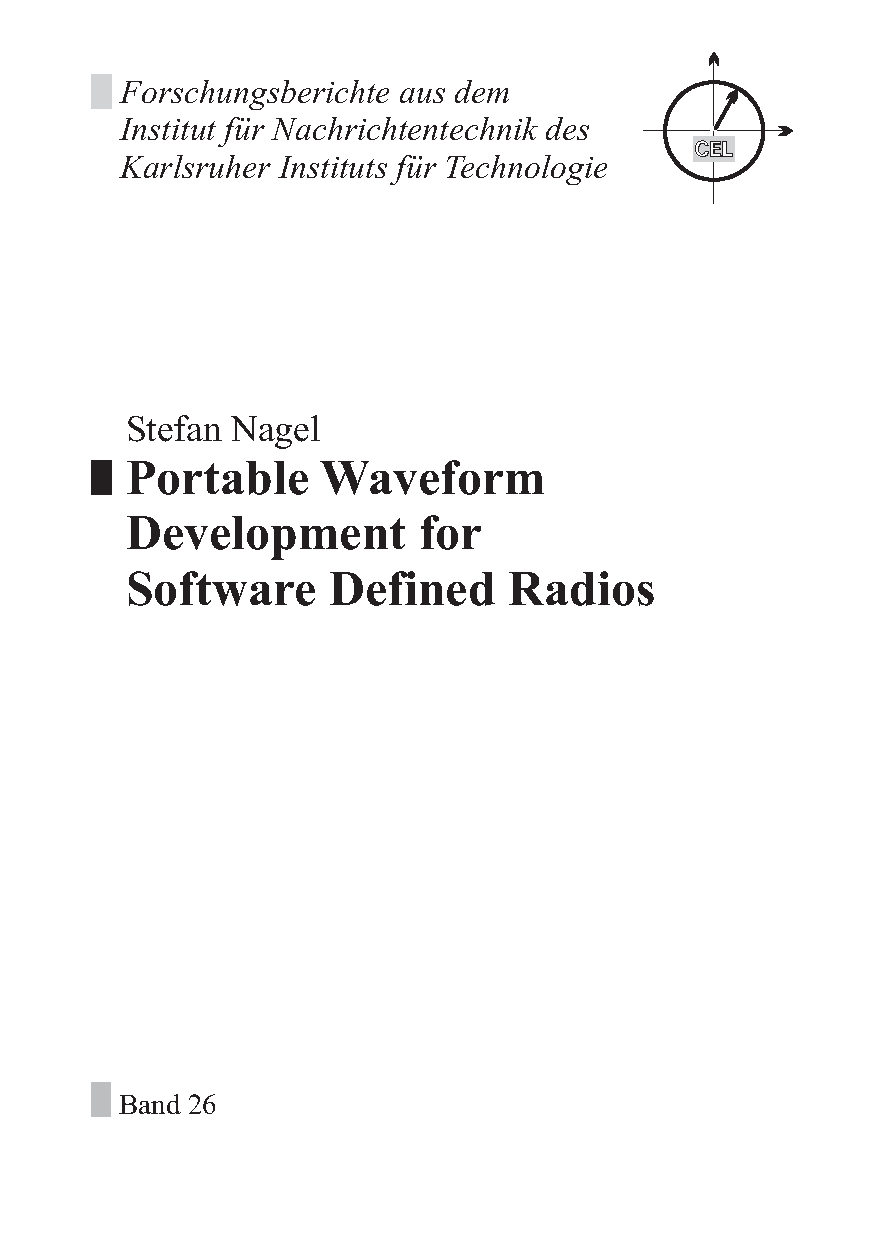
\includegraphics[]{../sonstiges/bilder/title.pdf}
%\end{figure}
%\clearpage

%%%%%%%%%%%%%%%%%%%%%%%%%%%%%%%%%%%%%%%%%%%%%%%%
% R�ckseite Schmutztitel

%%%%%%%%%%%%%%%%%%%%%%%%%%%%%%%%%%%%%%%%%%%%%%%%
%\thispagestyle{empty}
%\phantom{x}
%\vfill
%\begin{tabular}{@{}l@{ }l@{}}
%Copyright:&Institut f�r Nachrichtentechnik (CEL)\\
%&Karlsruher Institut f�r Technologie (KIT)\\
%&2011\\
%&\\
%Druck: & Frick Digitaldruck\\
%        &Br�hlstra�e 6\\
%        &86381 Krumbach\\
%&\\
%ISSN: & 1433-3821
%\end{tabular}
%\newpage

%\newcommand{\FBTableHead}{%
  \multicolumn{2}{@{}c@{}}%
  {\centering \bf Forschungsberichte aus dem Institut f�r Nachrichtentechnik}\\
  \multicolumn{2}{@{}c@{}}{\bf des Karlsruher Instituts f�r
    Technologie}\\ 
    \multicolumn{2}{@{}c}{Herausgeber: Univ.-Prof. Dr.\,rer.\,nat. Friedrich Jondral}\\
\rule{0pt}{3ex}  
  \\}
%
\begin{tabular}{@{}p{1.4cm}p{9.2cm}@{}}
  \FBTableHead%
Band 1&Marcel Kohl\\
  &{\bf Simulationsmodelle f�r die Bewertung von \newline Satelliten�bertragungsstrecken im
    \newline 20/30 GHz Bereich}\\
\rule{0pt}{3ex}%
Band 2&Christoph Delfs\\
  &\textbf{Zeit-Frequenz-Signalanalyse: Lineare und \newline quadratische
    Verfahren sowie vergleichende \newline 
    Untersuchungen zur Klassifikation von Klaviert�nen}\\%
\rule{0pt}{3ex}%
Band 3&Gunnar Wetzker\\%
  &{\bf Maximum-Likelihood Akquisition von Direct\newline Sequence Spread-Spectrum Signalen}\\
\rule{0pt}{3ex}%
Band 4&Anne Wiesler\\
  &{\bf Parametergesteuertes Software Radio \newline f�r Mobilfunksysteme}\\%
\rule{0pt}{3ex}%
Band 5&Karl L�tjen\\
  &{\bf Systeme und Verfahren f�r strukturelle \newline Musteranalysen
    mit Produktionsnetzen}\\\rule{0pt}{3ex}%
Band 6&Ralf Machauer\\
  &{\bf Multicode-Detektion im UMTS}\\\rule{0pt}{3ex}%
Band 7&Gunther M. A. Sessler\\
  &{\bf Schnell konvergierender Polynomial Expansion \newline Multiuser  Detektor mit niedriger Komplexit�t}\\
\rule{0pt}{3ex}%
Band 8&Henrik Schober\\
  &{\bf Breitbandige OFDM Funk�bertragung bei\newline hohen
    Teilnehmergeschwindigkeiten}\\\rule{0pt}{3ex}% 
Band 9&Arnd-Ragnar Rhiemeier\\
  &{\bf Modulares Software Defined Radio}\\\rule{0pt}{3ex}%
Band 10 & Mustafa Meng\"{u}\c{c} �ner\\
&{\bf Air Interface Identification for \newline Software Radio Systems}\\
\rule{0pt}{3ex}
\end{tabular}

\newpage
\begin{tabular}{@{}p{1.4cm}p{9.2cm}@{}}
 \FBTableHead
Band 11 & Fatih \c{C}apar\\
&{\bf Dynamische Spektrumverwaltung und  \newline elektronische
  Echtzeitvermarktung von \newline
Funkspektren in Hotspotnetzen}\\%
\rule{0pt}{3ex}%
Band 12 & Ihan Martoyo\\
&{\bf Frequency Domain Equalization in CDMA Detection}\\%
\rule{0pt}{3ex}%
Band 13 & Timo Wei\ss\\
&{\bf OFDM-basiertes Spectrum Pooling}\\%
\rule{0pt}{3ex}%
Band 14 & Wojciech Kuropatwi\'{n}ski-Kaiser\\
&{\bf MIMO-Demonstrator basierend \newline auf GSM-Komponenten}\\%
\rule{0pt}{3ex}%
Band 15 & Piotr Rykaczewski\\
&{\bf Quadraturempf�nger f�r Software Defined Radios: \newline Kompensation von Gleichlauffehlern}\\%
\rule{0pt}{3ex}%
Band 16 & Michael Eisenacher\\
&{\bf Optimierung von Ultra-Wideband-Signalen (UWB)}\hfill\\%
\rule{0pt}{3ex}%
Band 17 & Clemens Kl�ck\\
&{\bf Auction-based Medium Access Control}\\%
\rule{0pt}{3ex}%
Band 18 & Martin Henkel\\
&{\bf Architektur eines DRM-Empf�ngers \newline und
  Basisbandalgorithmen zur Frequenzakquisition \newline  und Kanalsch�tzung}\\%
\rule{0pt}{3ex}%
Band 19 & Stefan Edinger\\
&{\bf Mehrtr�gerverfahren mit dynamisch-adaptiver \newline Modulation
  zur unterbrechungsfreien \newline Daten�bertragung  in
  St�rf�llen}\\%
\rule{0pt}{3ex}%
Band 20 & Volker Blaschke\\
&{\bf Multiband Cognitive Radio-Systeme}\\
&\\\end{tabular}

\begin{tabular}{@{}p{1.4cm}p{9.2cm}@{}}
  \FBTableHead%
\rule{0pt}{3ex}%
Band 21 & Ulrich Berthold\\
&{\bf Dynamic Spectrum Access using OFDM-based \newline Overlay Systems}\\%
\rule{0pt}{3ex}%
Band 22 & Sinja Brandes\\
&{\bf Suppression of Mutual Interference in \newline OFDM-based Overlay  Systems}\\%
\rule{0pt}{3ex}%
Band 23 & Christian K{\"o}rner\\
&{\bf Cognitive Radio -- Kanalsegmentierung und  \newline Sch{\"a}tzung von Periodizit{\"a}ten}\\%
\rule{0pt}{3ex}%
Band 24 & Tobias Renk\\
&{\bf Cooperative Communications: Network Design and \newline Incremental Relaying}\\%
\rule{0pt}{3ex}%
Band 25 & Dennis Burgkhardt\\
&{\bf Dynamische Reallokation von spektralen Ressourcen \newline in
  einem hierarchischen Auktionssystem}\\
\rule{0pt}{3ex}%
Band 26 & Stefan Nagel\\
&{\bf Portable Waveform Development for \newline Software Defined Radios}\\
&\\\end{tabular} 

%\cleardoublepage

%\chapter*{Vorwort des Herausgebers}

%Software Defined Radios (SDRs) werden inzwischen seit zwei Jahrzehnten intensiv untersucht. Dabei stand zun�chst die Frage im Vordergrund, wie ein Funkger�t entwickelt werden kann, das mehrere verschiedene Standards unterst�tzt. Danach wurden in weitergehenden Untersuchungen Verfahren zum Software-Update, auch durch Funk�bertragung, implementiert. Dazu geh�rten auch Methoden zum Nachweis der Korrektheit der �bertragenen Software. Breitfl�chig durchgesetzt haben sich die SDR Technologien bisher im Wesentlichen in Basisstationsger�ten. Mobile Endger�te existieren vor allen Dingen als Multiband- (GSM 900, 1800, 1900) und Multistandard- (GSM, UMTS) Transceiver.

%Eine weitere wesentliche Eigenschaft, durch die sich SDRs auszeichnen k�nnen, wurde bisher zwar in der Literatur breit diskutiert, experimentell jedoch, wohl wegen der dazu notwendigen Hardware, nicht angegangen. Es handelt sich um die \textbf{Portabilit�t} von Wellenformen\footnote{Die Begriffe Standard und Wellenform werden oft als synonym angesehen. Allerdings umfassen Wellenformen, im Gegensatz zu Standards, h�ufig neben der Definition einer Luftschnittstelle auch Eigenschaften des Empf�ngers.} von einer Hardwareplattform auf eine andere. Durch das Aufkommen finanzierbarer Plattformen wie der Universal Software Radio Peripheral (USRP) von Ettus Research oder der Small Form Factor Software Defined Radio Development Platform (SFF SDR DP) von Lyrtech wird eine experimentelle Untersuchung der Portabilit�t von Wellenformen durchf�hrbar. Dabei treten Fragen nach einer Entwicklungsstrategie f�r die SDR Software unter Ber�cksichtigung der Portabilit�t sowie nach den Kosten, die eine Portierung verursacht, in den Vordergrund. Um hierf�r Antworten finden zu k�nnen, m�ssen, neben einem profunden Wissen �ber die beteiligten SDR Plattformen, Kenntnisse �ber Wellenformen bzw. Standards vorliegen. Dazu kommt die Beherrschung der notwendigen Hilfsmittel wie Programmiersprachen von MatLab �ber Python und C bis hin zu VHDL, Verilog und Assembler sowie der Umgang mit Messmitteln wie Signalgeneratoren und -analysatoren, die f�r den Nachweis erfolgreicher Arbeit, der die Interoperabilit�t zwischen auf verschiedenen Hardwareplattformen basierenden Funkger�ten umfasst, gebraucht werden.

A%uf der Basis des am KIT Institut f�r Nachrichtentechnik (Communications Engineering Lab, CEL) eingerichteten Funklabors hat Stefan Nagel die Portabilit�t verschiedener Wellenformen zwischen den beiden oben genannten Hardwareplattformen USRP und SFF SDR DP untersucht. Mit der Dissertation \emph{Portable Waveform Development for Software Defined Radios} legt er die wesentlichen Ergebnisse seiner Arbeit vor.

%Die Arbeit tr�gt insofern nachhaltig zum Fortschritt von Wissenschaft und Technik bei, als hier erstmalig, basierend auf der Model Driven Architecture (MDA) der Object Management Group (OMG), die Software f�r die Signalverarbeitung verschiedener Funk�bertragungsstandards entwickelt, implementiert und von einer Plattform auf eine andere portiert wurde. 


Karlsruhe, im 20XX\newline
Friedrich Jondral





%\cleardoublepage

\thispagestyle{empty}

\begin{center}

\vskip-3.55cm
{\vspace{1cm}
\huge Small Cell Deployment for Cognitive Radio\\
\vskip0.25cm
}

\vfill


\vskip1.0cm

Zur Erlangung des akademischen Grades eines 
\vfill

\vskip0.5cm
{\large DOKTOR-INGENIEURS}
\vskip0.5cm
\vfill

von der Fakult�t f�r

Elektrotechnik und Informationstechnik

des Karlsruher Instituts f�r Technologie
\vfill

\vskip0.5cm

genehmigte
\vfill

\vskip0.5cm

{\large DISSERTATION}
\vfill

\vskip0.75cm

von
\vfill

\vskip0.75cm

{\large M.Sc. Ankit Kaushik}
\vskip0.75cm



geb. in



\vskip0.15cm
\vfill


Neu Delhi, Indein

\vfill
\vskip0.75cm

\todo{Date and coreferent}
\phantom{tabula}
\begin{tabular*}{11.1cm}{@{}l@{\extracolsep\fill}r@{}}
Tag der m�ndlichen Pr�fung:&\hfill XX 20XX\\
Hauptreferent:&\hfill Univ.-Prof. Dr.\,rer.\,nat. Friedrich K. Jondral\\
Korreferent:&\hfill Prof. M�setermann\\
\end{tabular*}
 \end{center}

\cleardoublepage

\chapter*{Summary}
%Der Grundgedanke bei Software Defined Radios besteht darin, Funkstandards in Software auf rekonfigurierbaren Prozessoren zu verarbeiten. Dieses Konzept f�r neue Funkger�te existiert bereits seit mehreren Jahrzehnten. Allerdings ist es erst durch die rasante Entwicklung auf dem Markt der Prozessoren der letzten Jahre m�glich, SDR-Plattformen kommerziell zu erwerben und eigene Wellenformen zu implementieren. Dabei ergibt sich das Problem, dass Wellenformen, die auf der eigenen Plattform lauff�hig sind, zu anderen Plattform nicht zwangsl�ufig kompatibel sind. Dieses Problem tritt  auch bei einer m�glichen Platt\-formerneuerung auf. Die Wellenformen, die f�r eine alte Plattform entwickelt wurden, m�ssen auf eine neue Plattform portiert werden. Dabei stellt sich zwangsl�ufig die Frage: ,,Wie k�nnen Wellenformen entwickelt werden, die auf beliebigen Plattformen lauff�hig sind?''

%Ein Erfolg versprechender Ansatz ist die Entwicklung von Wellenformen nach der Model Driven Architecture. Diese beschreibt einen Entwicklungsprozess, der sich von sehr generischen, plattformunabh�ngigen Modellierungen der Funktionalit�t bis zum ausf�hrbaren Bin�rcode erstreckt. In dieser Arbeit wird vorgestellt, wie dieser Prozess auf die portable Entwicklung von Wellenformen angepasst werden kann. Die automatisierte Erzeugung von Quellcode spielt hierbei eine wichtige Rolle. Daher werden Laufzeit- und Speichermessungen vorgestellt, die generierten Code mit nicht optimiertem und optimiertem Code vergleichen  und damit einen Einblick in die Effizienz von automatisch generiertem Code erlauben.

%Das Ettus USRP und das Lyrtech Small Form Factor SDR geh�ren zu den kommerziell erfolgreichsten SDR-Plattformen. Daher werden in dieser Arbeit ausf�hrlich ihr Aufbau sowie ihre F�higkeiten und Limitierungen beschrieben. Weiterhin wird aufgezeit, wie diese Plattformen in den be\-reits vorgestellten Entwicklungsprozess integriert werden k�nnen. Dazu geh�ren sowohl die Umsetzung der programmierbaren Schnittstellen und der Bussysteme in die Systemmodellierung als auch die Integration der betreffenden Prozessoren in die Codegenerierung.

%Um zu demonstrieren, dass der vorgestellte Entwicklungsprozess auch praktisch anwendbar ist, wurde die Wellenform TETRA f�r eine Platt\-form entwickelt und auf eine zweite Plattform portiert. Die Umsetzung der dabei zu realisierenden Modelle werden in dieser Arbeit genauso vorgestellt wie die Verarbeitungsdauer der Algorithmen auf den betreffenden Prozessoren. Um zu gew�hrleisten, dass die Wellenform standardkonform umgesetzt wurde, kamen Messger�te zum Einsatz, die sowohl Sende- als auch Empfangspfad gegen die TETRA-Spezifikation getestet haben. Neben TETRA wurden zwei weitere Wellenformen ent\-wickelt und portiert. Die Ergebnisse und Herausforderungen all dieser Entwicklungsvorg�nge werden in dieser Arbeit pr�sentiert.
   

  

\cleardoublepage

\chapter*{Abstract}

%The basic idea of Software Defined Radio is the implementation of radio communication standards with software on reconfigurable processors. This concept for new radio devices was already proposed several decades ago. However, through the rapid development of processors in recent years, it is possible to acquire commercial SDR platforms and build own waveforms. Unfortunately, waveforms that are developed for one platform are not necessarily compatible to other platforms. This problem also occurs with a possible hardware upgrade. The waveforms that were developed for an old platform must be ported to a new platform. Therefore, this work focuses on the question: ``How can we build waveforms that can be moved from one platform to another?''

%A promising approach is the development of waveforms based on the Model Driven Architecture. It describes a development process that extends from a very generic, platform-independent functionality to the executable binary code. This work presents the adaption of this process to the development of portable waveforms. In this process, the automated generation of source code plays a decisive role. Therefore, measurements of processing time and memory consumption are presented to compare the generated code with non-optimized and optimized code and allow insights into the efficiency of automatically generated code.

%The USRP from Ettus and the Small Form Factor SDR from Lyrtech are among the most used commercially SDR platforms. Therefore, their structure as well as their capabilities and limitations are presented in this work. It is furthermore shown, how these platforms can be integrated into the development flow. This includes the implementation of programmable interfaces and bus systems as well as the integration of the processors in the code generation process.

%To demonstrate that the used development flow is also applicable in practice, a proof of concept is given with the development and port of a TETRA waveform from one platform to another. Therefore, the realizations of the waveform for both platforms are presented as well as the processing times for the algorithms on the different processors. To demonstrate the standard compliance, the waveform was tested with measurement equipment against the TETRA air specification. In addition to TETRA, two other waveforms were developed and ported. This work presents the results and challenges of all these waveform developments and ports.


\cleardoublepage







%% Inhaltsverzeichnis %%%%%%%%%%%%%%%%%%%%%%%%%%%%%%%%%%%%%%%
\tableofcontents %Table of contents


%% Chapters %%%%%%%%%%%%%%%%%%%%%%%%%%%%%%%%%%%%%%%%%%%%%%%%%
\mainmatter

\chapter{Introduction}
\label{chap:Int}

Since the invention of smart devices, the mobile traffic has been increasing tremendously over the last decade. According to the recent surveys on mobile traffic by prominent market leaders (Cisco \cite{CISCO14} and Ericsson\cite{Eric15}), the existing mobile traffic is expected to increase $11$-fold  by 2021. The wireless community including the standardization bodies (3GPP \cite{3GPP}) believe that the state-of-the-art standards (\index{fourth-Generation (4G)} -- \index{LTE}, \index{WiMAX}) are not capable of sustaining these ever-increasing demands in the upcoming decade. With this situation in hand, the standardization bodies are currently in the phase of conceptualizing the requirements of the \index{fifth-Generation (5G)} of mobile wireless systems.
Some of these major requirements are: (i) areal capacity in $\SI{}{bits/sec/m^2}$ must increase by a factor of $1000$ compared to 4G, (ii) low latency of approximately \SI{1}{ms}, and, (iii) energy- and cost-efficient deployment \cite{Qual13, Andrews14}.
 %One of the major goals is to improve the areal capacity ($\SI{}{bits/s/m^2}$) by a factor of 1000 \cite{Qual13, Andrews14}. \tc{To this end, an extension to the already allocated spectrum is of paramount importance.} 
The feasibility of these requirements can be envisaged through the application of promising approaches such as maximization of the spatial degrees of freedom -- using massive MIMO \cite{Lar14} and 3D-beamforming \cite{Hal13} --, \index{in-band full-duplex communications} \cite{Sab14}, small cell densification \cite{Andrews12, Gel13}, alternatives to the already allocated spectrum -- such as millimeter-Wave technology (mmW) \cite{Rapp13}, visible light communications \cite{Wu14} and Cognitive Radio (CR) communications -- and waveform design \cite{Scha14, Baz15}, \figurename~\ref{fig_Int:5G} describes a classification of these approaches. In order to narrow down the perspective, in this thesis, a deployment scenario that lays emphasis on the small cell densification and the implementation of CR techniques is proposed. Before any further advancement, the underlying facts are elaborated that make small cell densification and CR communication approaches, particularly their combination, a suitable candidate for the 5G networks. 

\begin{figure}
\centering
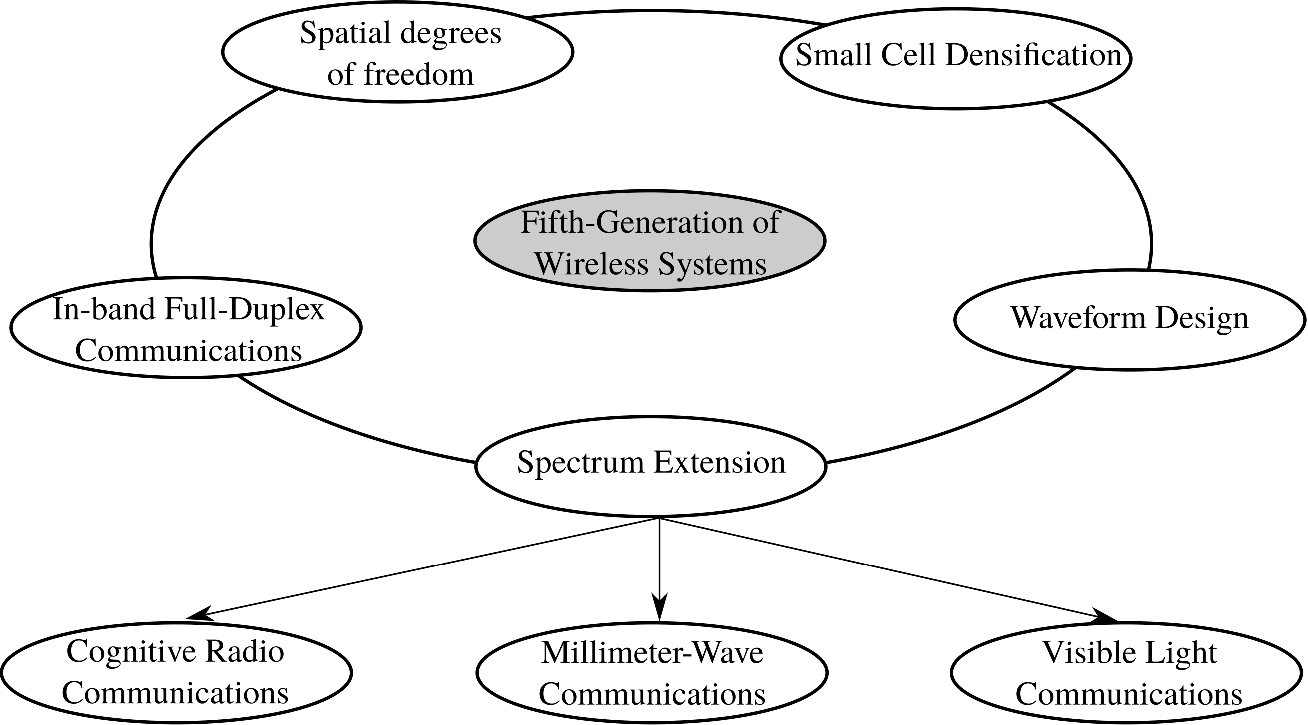
\includegraphics[width = 0.98 \columnwidth]{figures/5G}
\caption{An illustration of the potential approaches considered under the 5G framework.}
\label{fig_Int:5G}
\end{figure}


\subsubsection*{\index{Small Cell Densification}}

In the recent past, Small Cells (SCs) have emerged as a potential solution for coverage and capacity enhancements inside a wireless network. A SC represents a low power station that ranges from $\SI{10}{m}$ to $\SI{100}{m}$. The reduced transmit distance accomplished with the deployment of SCs enhances the link quality and aids spatial reuse \cite{Chander08}.
%SC is particularly deployed in a indoor or outdoor environments, these include enterprise, shopping complex or residential \cite{SSF14}. 
As a result, small cell densification can leverage the areal capacity of a 5G network \cite{Andrews14}. The capacity, however, increases linearly with the number of SCs, it is infeasible to procure the factor of $1000$ in the areal capacity with densification alone. In addition, the operation and the integration of these substantial number of SCs to the backhaul network are cost- and energy-intensive for the mobile operator, which limits the degree to which the densification can be achieved by a wireless network.





\subsubsection*{Spectrum extension}
Complementing the link quality by means of SCs, the spectrum %\footnote{The spectrum corresponds to the radio frequency.} 
represents a major contribution to the desired areal capacity. Considering the present allocation of the spectrum below $\SI{6}{Hz}$ to different wireless services, it is difficult to procure an extension to the already available spectrum to the mobile communication. Before investigating the potential candidates for the spectrum extension, it is necessary to consider the following classification of the spectrum:
%\begin{itemize}
(i) $> \SI{6}{GHz}$;
(ii) $\le \SI{6}{GHz}$.
%\end{itemize}
The prime objective of this sort of classification is to shift the focus on the propagation characteristics and the issues thereof.


The spectrum beyond \SI{6}{GHz} largely entails the mmW, which is well-known for point-to-point communications. Recently, it is envisaged as a powerful source of spectrum for 5G wireless systems. However, the mmW technology is still in its initial stage and along with complex regulatory requirements in this regime, it has to address several challenges like propagation loss, low efficiency of radio frequency components such as power amplifiers, small size of the antenna and link acquisition \cite{Rapp13}. Therefore, in order to capture a deeper insight of its feasibility in 5G, it is essential to overcome the aforementioned challenges in the near future.\nociteK{Kaushik13, Kaushik14_W, Kaushik14_CC, Kaushik14_P, Kaushik15_CC,Kaushik15_ICC, Kaushik15_D, Kaushik16_TWC, Kaushik16_VTC1, Kaushik16_TCCN, Kaushik16_ICC, Kaushik16_CC, Kaushik16_VTC2, Kaushik17}

\begin{figure}[!t]
\centering
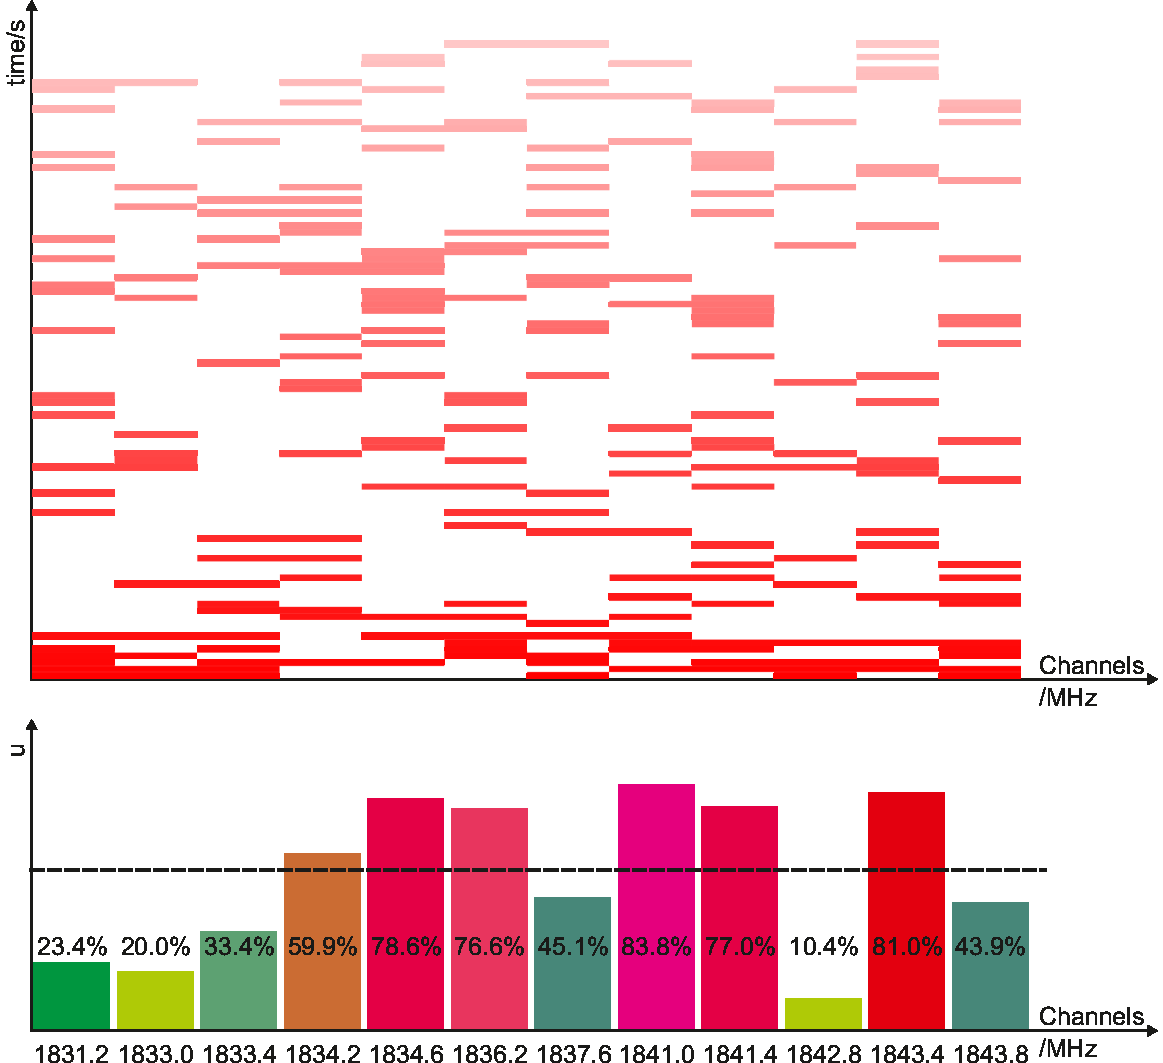
\includegraphics[width = 0.9\columnwidth]{figures/Grafik_Poster}
\caption{A snapshot of a hardware demonstrator that measures the spectral occupancy in GSM \SI{1800}{MHz} downlink channels, whereby the slices (red and white) represent the spectrum occupancy (1 or 0) corresponding to a single measurement at a given time instant. The bar plots illustrate the spectrum occupancy (u) for each channel with a history of 500 measurements\protect\citeK{Kaushik13}.}
\label{fig_Int:HW_I}
\end{figure}


Besides the spectrum beyond \SI{6}{GHz}, an efficient utilization of the spectrum below \SI{6}{GHz} presents an alternative solution. The use of the spectrum in this regime (below \SI{6}{GHz}) is fragmented and statically allocated \cite{Mchen05, Mchen07}, leading to inefficiencies and the shortage in the availability of the spectrum for new services. To support this argument that the spectrum is underutilized, a glimpse of the measurement campaign is presented in \figurename~\ref{fig_Int:HW_I}. The measurements, acquired during the peak hours, illustrate the spectrum occupancy for the GSM \SI{1800}{MHz} downlink sub-channels. The low spectrum occupancy for most of the sub-channels clearly signifies the fact that the demand for the additional spectrum can be fulfilled only by managing the utilization of the available spectrum efficiently. 

In this perspective, CR is foreseen as one of the potential contenders that addresses the spectrum scarcity problem. Since its origin by Mitola \textit{et al.} in 1999 \cite{Mitola99}, this notion has evolved at a significant pace, and consequently has acquired certain maturity. Despite the existence of the theoretical analysis, from a deployment perspective, this technology is still in its preliminary phase \cite{Pawe11}. In order to curtail the gap between the theoretical models and the practical implementations, recently, the wireless community has started to show an inclination\footnote{As indicated by the increased promotion for hardware implementation/demonstration or performing events such as spectrum challenge\citeK{Kaushik15_D} in conferences like IEEE DySPAN.} towards models and/or techniques. Hence, enabling the placement of this concept over a hardware platform so that the disposition of CR systems in the upcoming 5G wireless networks can be facilitated. Motivated by this fact, this thesis focuses on the performance analysis of CR systems from a deployment perspective. 

In contrast to the Radio Frequency (RF) spectrum, Visible Light Communication (VLC) has started to gain extensive attention for 5G wireless communication, hence, deserves consideration in context to spectrum extension. Despite the fact that VLC offers some attractive characteristics like spatial, spectrum reuse, low energy efficiency and security, it has to overcome certain challenges such as mobility and adverse effect of atmospheric conditions while operating outdoor \cite{Wu14}. 


\section{Background and Motivation}
\label{sec:mot}

\subsubsection*{\index{Cognitive Radio Systems}}


In order to proceed further, it is essential to understand the classification of different CR systems described in the literature. An access to the licensed spectrum is an outcome of the paradigm employed by a Secondary User (SU). In this context, all CR systems that provide shared access (used interchangeably with secondary access) to the spectrum mainly fall under the following categories \cite{Goldsmith09}, please consider \figurename~\ref{fig_Int:paradigm} for a graphical illustration of different CR systems and their corresponding techniques considered in the thesis\footnote{A detailed investigation of these techniques is provided in the following chapters.}. 
\begin{itemize}
\item According to \index{Cognitive Radio Systems!Interweave System} (IS), the SUs render an interference-free access to the licensed spectrum by exploiting spectral holes in different domains such as time, frequency, space and polarization. 
\item Underlay System (US) enable an interference-tolerant access, according to which the SUs are allowed to use the licensed spectrum (e.g. Ultra Wide Band (UWB)) as long as they respect the interference constraints of the Primary Receivers (PRs). 
\item \index{Cognitive Radio Systems!Hybrid System} (HS) combine the benefits of the IS (agility to detect spectrum holes in different domains) and the US (interference-tolerant capability) so that the spectrum available for performing secondary access can be used efficiently.  
\item \index{Cognitive Radio Systems!Overlay system} consider advanced transmission and coding strategies, which include the participation of higher layers for enabling the spectral coexistence between two or more wireless networks. 
\end{itemize}
The IS, the US and the HS are closely associated with the physical layer, hence, these systems are mostly considered not only for the theoretical analysis but for practical implementations as-well \citeK{Kaushik13,Kaushik14_CC,Kaushik15_D, Kaushik16_CC, Kaushik16_VTC2}, \cite{Cabric04, Cabric06, Kim10}. 
Underlying this fact, this thesis establishes a deployment-centric viewpoint for characterizing the performance of these CR systems. In order to illustrate a successful incorporation of the CR techniques in a 5G network, a specific use-case (deployment scenario) is presented subsequently. 


\begin{figure}
\centering
\includegraphics[width = 0.85 \columnwidth]{figures/CR_paradigm}
\caption{A classification of different CR systems and their corresponding techniques that allow shared access to the licensed spectrum.}
\label{fig_Int:paradigm}
\end{figure}



\subsection{Cognitive Small Cell: A Prominent Use-Case}
\begin{figure}
\centering
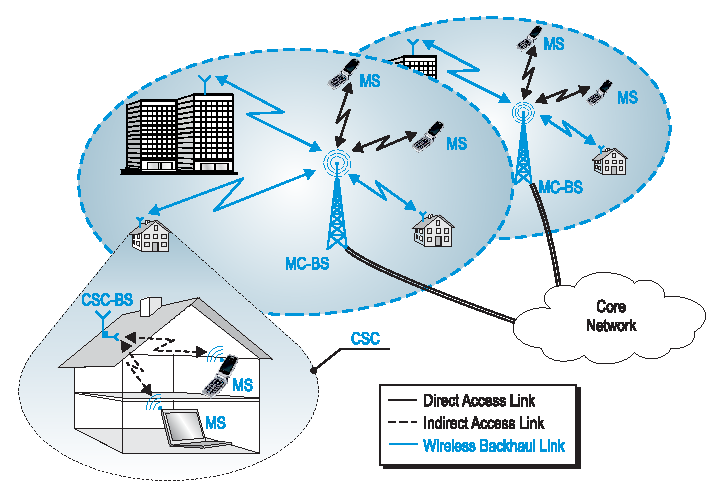
\includegraphics[width = 0.9 \columnwidth]{figures/Cellular_Scenario_CR6F}
\caption{An illustration of the CSC deployment in a 5G network.}
\label{fig_Int:archi}
\end{figure}



It is evident from the previous discussion that the spectrum extension via CR systems and SC densification are significant to the 5G system. %Recently, ElSawy \textit{et al.} \cite{Elsawy13} have presented Cognitive Small Cell (CSC), a concept that fulfills the capacity demands of the future wireless networks. 
Based on this, a preliminary concept of Cognitive Small Cell (CSC), a promising application that combines the benefits from the SC deployment and the efficient usage of the spectrum below \SI{6}{GHz} by implementing CR techniques to accomplish the requirements of 5G networks is presented. A typical scenario where the CSC finds its application would be the co-existence of Wi-Fi or unlicensed small cell and wireless cellular systems \cite{Benn13, Gali15}. The notion of CSC has been previously investigated by Elsawy \textit{et al.} \cite{Elsawy13, Elsawy13_cmag} and Wildemeersch \textit{et al.} \cite{Wild13}, where the authors primarily emphasized on the modelling techniques\footnote{The modelling is based on stochastic geometry, which allows a spatial averaging over multiple network geometries \cite{Haenggi, Haenggi08now}.} that depict the positioning of several CSCs inside the network. Due to this, the performance analysis of the CSC has been limited mainly to network abstraction. In contrast, this thesis emphasizes on fundamental aspects encountered while deploying a CSC, which otherwise could forbid its realization over the hardware. %, which could possibly lead to a successful integration of CSCs in the 5G network. %Consequently, by considering different CR paradigms to enable secondary usage of the licensed spectrum, here a deeper comprehension of the concept is illustrated. %, thereby, making it accessible to 5G systems. 
%To strengthen our understanding of CSC, we demonstrate the feasibility of the respective paradigms by means of hardware implementations.
%Pertaining to the deployment, we analyze the true performance of the CSC as a CR application for the mentioned paradigms.  
 A comprehensive incorporation of CSC in a preliminary 5G architecture is illustrated in \figurename~\ref{fig_Int:archi}. In order to enhance the viability of the proposed network architecture, it is interesting to highlight some of the essential ingredients pertaining to the deployment of the CSC.

\subsubsection*{Network Elements}
 In order to propose a successful integration of CSC in a 5G network, the following key elements are essential: a CSC-Base Station (CSC-BS), a Macro Cell-Base Station (MC-BS) and Mobile Stations (MSs), cf. \figurename~\ref{fig_Int:archi}. MSs are the devices either served by the MC-BS over a \textit{direct access} link or the CSC-BS over an \textit{indirect access} link. The direct access and the indirect access are the nomenclature used to distinguish a start-of-the-art (spectrum) access between the MC-BS and the MS from an access between the CSC-BS and the MS representing a CR communication, respectively. Furthermore, the MC-BS is connected to several CSC-BSs over a \textit{wireless backhaul} link. Although the MC-BS and the MS already exist in the conventional cellular architecture, to incorporate the opportunistic access inside the CSC, it is necessary to consider a functionality upgrade.

\subsubsection*{Spectrum Access}
In the proposed network architecture, the access to the spectrum is realized over the wireless backhaul, the direct access and the indirect access links, cf. \figurename~\ref{fig_Int:archi}.
\begin{enumerate}
\item A wireless backhaul is a
%quasi-line of sight\footnote{It allows limited number of objects between the direct link.} 
point-to-point wireless link between the CSC-BS and the MC-BS that relays the traffic generated from the CSC to the core network. Accounting the densification of the CSC in 5G network, the wireless backhaul link, in contrast to the optical fiber link, presents a cost-effective and energy-efficient alternative to the mobile operator.
With the limited infrastructure required for deployment, it accelerates the installation process and promotes scalability of the network.
For the wireless backhaul link, an exclusive spectrum for a longer duration is desired. Hence, it is sensible to nominate a mmW band; alternatively, an exclusive band below \SI{6}{GHz} can be acquired using the principles of Licensed Shared Access (LSA) \cite{ETSI13}.
%These WB links encourage ultra-densification as they brings down the capital expenditure and offer scalability to the vendor. 

\item A direct access link represents a direct access of the MS at the MC-BS over the allocated spectrum. Consequently, the spectrum access for this link is analogous to the one existing in the state-of-the-art wireless standards.
\item The CSC elements (the CSC-BS and the MS) are responsible for executing the secondary access to the licensed spectrum. The additional spectrum acquired is used for the communication between the CSC-BS and the MS over the indirect access link.
\end{enumerate}

\subsubsection*{Network Compatibility}
Besides secondary access, CSC has to co-exist harmoniously with the other elements existing in the network. In this context, the network elements are embedded with additional functionality such as:
\begin{itemize}
\item The MS procures the control information (signalling and synchronization) over the indirect access link after connecting to the near-by CSC-BS.
\item In order to accomplish a logical placement of CSCs inside the network, the CSC employs S1 and X2 interfaces over the wireless backhaul link.
%Under this situation, the MC-BS, however, remains transparent to the additional spectrum acquired by the CSC over the IA link. 
%For the co-exisitence it is necessary to consider the co-existence of CSCs under the MC. 
\item For situations where several CSC-BSs co-exist under a MC-BS, operations like seamless cross-tier and co-tier mobility constitute a challenging task for the network.
\end{itemize}


\subsubsection*{Hardware Feasibility}
Along with other ingredients, it is essential to outline certain aspects that pertain to the hardware realizability of the CSC. For the CSC-BS, an antenna mount system consisting of an indoor and an outdoor antenna is proposed. Whereby, the indoor antenna exploits the walls of the building to physically separate the indoor transmissions over the indirect access link, in this way, it curtails the interference to the primary system and to the neighbouring CSCs, vice-versa. Whereas, the outdoor antenna secures a narrow beam transmission to enhance the link quality for the wireless backhaul link. Besides this, it is a well-known fact that Software Defined Radio (SDR) has played an important role in the genesis of the CR \cite{Jondral05}. Which means that the SDR can serve as a suitable platform for executing CR techniques, accomplishing rapid prototyping for the CR systems. Taking this into account, the SDR platform is utilized for realizing (or demonstrating) the CR functionality pursued by the CSC-BS over a hardware.


\subsubsection*{Indoor Deployment}
From a market survey, it has been depicted that $70\%$ of the mobile traffic is originated from indoor locations \cite{Chander08}. Another survey of the leading WiMAX operators revealed that $80\%$ of their subscribers will be connected indoors \cite{Pao07}. In addition, a new range of wireless services, categorized as Internet of Things, will operate indoors. Following these facts, it is clear that the performance gains in terms of spectrum reuse will be far more consequential if we manage to consolidate these sources of traffic by means of SCs deployment. Hence, it is sensible to consider the residential and enterprise as the main deployment scenarios for the CSC, cf. \figurename~\ref{fig_Int:archi}. Except for a different coverage regime, the operating principles of these scenarios are analogous. Besides, in context with the CR, where the interference mitigation between the primary and the secondary systems is a significant aspect, exercising the CR communication within the walls (which attributes to an indoor deployment) provides a spatial separation between the two systems. This, however, does not indicates that CR communication is limited to indoor scenarios. As the matter of fact, the indoor deployment is opted \begin{itemize} \item to exploit the behavioral dimension of the traffic source (traffic management) and \item to the mitigate interference between the two systems \end{itemize} so that co-existence with the licensed users is encouraged. 
In this regard, an indoor scenario is considered for the deployment of the CSC, cf. \figurename~\ref{fig_Int:archi}.  

\subsection{Performance Analysis}
Since the evolution of wireless systems, understanding the performance of novel algorithms/techniques related to the wireless systems has always been a challenging task. With regard to this, for a CR system, because of the involvement of two different systems, namely primary and secondary systems, this task is even more difficult. On one end, it has been engaging a large number of researchers that are eager to find solutions for the new set of problems that are emerging from an interplay between these two systems, leading them to develop theoretical models (system models). As a result, these models allow us to determine the performance limits of the CR system. However, to sustain analytical tractability, they tend to consider assumptions that in most situations are unrealistic for a hardware deployment.  %However, with the lack of concrete guidelines, different perspective have forward for the performance analysis.
 On the other end, due to the co-existence of the two systems sharing the same spectrum, the performance of a CR system is critical to the regulatory bodies and the mobile operators\footnote{These operators are the ones who are willing to share their license (as primary system) or the ones who are willing to access the licensed spectrum (as secondary system).}, responsible for managing the spectrum. In this regard, despite the numerous theoretical models that exist in the literature, when it comes to judging the performance of a CR system, the regulatory bodies give more preference to the hardware implementations that offer complete solutions. 

These different mindsets and the lack of proper guidelines ultimately lead to a mismatch between the two communities, and consequently slow down the evolution of the CR in realistic scenarios. Under this situation, it is advisable to merge these mindsets and establish a deployment-centric viewpoint towards the CR systems, according to which the upcoming models and/or techniques not only associate themselves to the performance characterization but are eligible for practical implementations as-well. This viewpoint, also the main motivation behind this work, is emphasized throughout the thesis. 

The co-existence between the primary and the secondary systems can be accomplished only through a detailed analysis of the performance of these systems. %The lack of proper guidelines defining these systems and their co-existence leave the performance analysis of the CR systems a challenging task. 
To address this issue, the researchers have made an intensive effort to develop system models \cite{Liang08, Kang209, Kang09}\footnote{For the sake of brevity, only limited works from the literature representing the performance analysis have been cited in this chapter. The following chapters corresponding to different CR systems consider an in-depth analysis of the related work.} that characterize the performance of the CR systems. The performed analysis boils down to the fact that the CR systems are allowed to successfully co-exist with the primary system only if they respect the interference at the primary system caused due to an access to their spectrum. This constraint defined by the primary system or the regulatory bodies allows us to effectively regulate the interference to the primary system. 

With regard to this constraint on the interference, the CR system intends to deliver a certain Quality of Service/Quality of Experience (QoS/QoE) in the form of throughput to their corresponding Secondary Receiver (SR), defined as \textit{Secondary throughput}. Such a QoS/QoE provisioning allows us to determine the potential applications or prominent use-cases for the CR system. For instance, after obtaining the throughput over the access link allows the CR to execute a band allocation policy, based on which the CR is able to relinquish those channels that ineffectively contribute to the secondary throughput but also are responsible for causing interference at the primary system. As a result, the performance of a CR system can be jointly characterized in terms of the harmful interference received at the primary system and the throughput achieved by the secondary system. 
%Because of such intricacies that are inherent to a CR system, its performance analysis have always been an interesting challenge. 
But the fact is, the derived expressions depicting the performance of the CR systems are rarely examined under realistic scenarios or implemented over the hardware mainly because of the complicated deployment scenario or the computational complexity of the employed CR techniques, leaving the validity of the existing theoretical analysis questionable. Taking this issue into account, this thesis analyzes the performance of the CR systems while putting emphasis on the fact that the performed analysis can be easily validated through a hardware implementation. 

\subsection{Imperfect Channel Knowledge for CR systems}

In a nutshell, \textit{a CR is an agile system that possesses the ability to adapt to the changes in the environment}. From a physical layer perspective, this corresponds to the response to the changes incurred from the system or the outside environment, leading to performance enhancement (or reducing performance degradation). Inherent to the wireless systems, these changes may arise due to the variations in the signal caused by the presence of the thermal noise at the receiver and the fading in the channel. It is well-known from the text-books, related to wireless communications \cite{simon2005, Goldsmith05, Tse05}, that the channel fading, in particular, is critical for wireless systems. As a matter of fact, channel knowledge -- in the form of Channel State Information at the Transmitter (CSIT) available through a feedback from the receivers -- has rendered a substantial improvement in the performance in terms of data rate, for instance, multiplexing gains for a MIMO system \cite{Ali12}. 


\begin{figure}[!t]
\centering
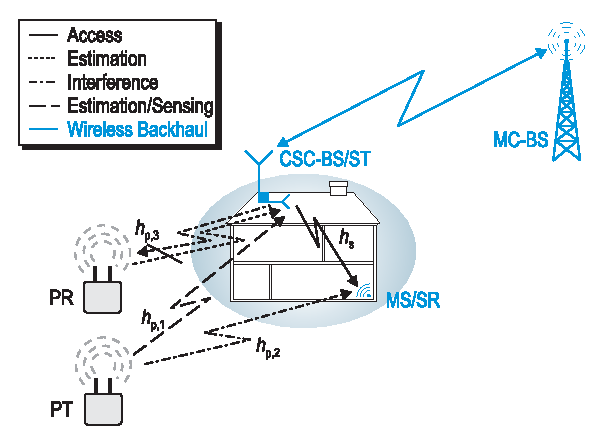
\includegraphics[width = \figscalet]{figures/CR_Scenario_Hybrid}
\caption{A cognitive small cell scenario demonstrating: (i) the CR systems employed at the CSC-BS, (ii) the associated network elements, which constitute Cognitive Small Cell-Base Station/Secondary Transmitter (CSC-BS/ST), Mobile Station/Secondary Receiver (MS/SR), Macro Cell-Base Station (MC-BS) and Primary Transmitter (PT), (iii) the interacting channels: sensing ($\hpo$), interference ($\hptw, \hpth$) and access ($\hs$) channels.}
\label{fig_Int:scenario}
%\vspace{-6mm}
\end{figure}


In context with a CR system, the channel knowledge, unlike the conventional or state-of-the-art wireless systems, is not confined to a single transmitter-receiver link, rather it includes all the related channels that exist within as-well-as across the primary and the secondary systems, cf. \figurename~\ref{fig_Int:scenario}. At this stage, it is worth understanding the fact that channel knowledge is paramount for the hardware implementation of the CR systems, since it allows them to exercise different techniques, cf. \figurename~\ref{fig_Int:paradigm}, and to respect the desired constraints, which are necessary for the their co-existence with the primary systems. 

From a theoretical perspective, the performance characterization of the CR systems demands the knowledge of the channels between these two systems. Absence of this knowledge, especially of those channels that are related to the interference at the primary systems, renders the performance characterization of a CR system inadequate for the practical implementations. Despite the existence of multitude of analytical models in the literature (ISs -- \cite{Liang08, Sharma14, Pradhan15}, USs -- \cite{Xing07, Ghasemi07, Kang09}, HSs -- \cite{Song13, Gmira15, Jiang13, Fili15}) that consider with the performance analysis of a CR system, its performance with regard to the channel estimation, due to the complexity of the underlying problem, has never been completely understood\footnote{In context to the US, certain works \cite{Musa09, Suraweera10, Kim12} have dealt with the issue of channel estimation in a CR system, however, unlike this thesis, the investigation has not been exhaustive. This issue is extensively outlined in Chapter \ref{chap:US} under the section ``Related Work''.}. In order to curtail this gap, this thesis capitalizes on the estimation of the involved channels in a CR system. In this sense, the accessibility of the channel knowledge at the CSC-BS facilitates the implementation of the CR techniques at the CSC-BS, enabling a CR communication link with the MS over the acquired spectrum. At the same time, this knowledge allows us to regulate the interference at the PR below a desired level. 

Certainly, an access to the channels' knowledge comes at a certain cost. Firstly, the inclusion of channel estimation demands an allocation of a certain time interval by the CSC-BS. In consideration to the time allocation, a certain degradation in the performance in terms of the throughput is obvious. Secondly, the variations introduced due to the estimation process, also treated as imperfect channel knowledge, lead to an uncertainty in the interference defined as \textit{uncertain interference}\footnote{The uncertain here specifically symbolizes the variations in the interference power received at the PR that exists because of the imperfect channel knowledge.} to the primary systems. If not considered, this uncertain interference may severely degrade the performance of the CR systems. In order to approach a successful integration of channel estimation into the CR system, it is essential to consider the performance degradation due to the time allocation and the uncertain interference in the system model, which are not addressed in the existing models that consider the perfect knowledge of the involved channels. This thesis takes these effects into account to establish analytical frameworks (each for the IS, the US and the HS) that allow us to understand the behaviour of the CR systems under those situations that are much closer to the realistic scenarios. %Subsequently, these frameworks are utilized to characterize the performance of the respective CR systems. 

Shifting the focus back to the deployment, it is worthy to understand that the channel estimation facilitating shared access to the licensed spectrum is viable only if the CR system is equipped with the knowledge about to the primary system, thus, it is dependent on the wireless standard followed by the primary system. This signifies that to perform channel estimation based on conventional techniques -- such as training-based \cite{Stoica03}, pilot-based \cite{Gifford05, Gifford08}, signal to noise ratio-based \cite{Chav11, Sharma13} channel estimation, which already exist in the literature -- a preliminary processing in the form of synchronization and demodulation of the baseband signal received from the primary system is necessary. The existence of multiple wireless standards and their complexity preclude us from deploying a dedicated circuitry corresponding to each primary system \cite{Ghasemi08_cm}. The fact is, these conventional channel estimation techniques are well-known for delivering accurate channel estimates, that is why employed in state-of-the-art wireless standard. In context with the CR systems, these techniques \begin{itemize} \item increase the complexity related to the channel estimation, evaluated in terms of the mathematical operations and (or) \item demand the demodulation of the Primary User (PU) signal. \end{itemize} 

Under these circumstances, it is advisable to consider only those solutions that offer low complexity and show versatility towards different PU signals. Generally speaking, such solutions will not only ease the deployment process but also have a large acceptance among the CR community. For instance, energy-based detection (or energy detection) has been a popular choice compared to its counterparts such as matched filtering-based and cyclostationary-based detection for detecting a PU signal, required for performing spectrum sensing for the interweave systems (discussed later in Chapter \ref{chap:IS}). A direct comparison of these techniques by counting their implementations for hardware demonstration has been done in \cite{Pawe11}. On similar grounds as energy detection, in order to approach the channel estimation for the CR system, particularly for the channels that involve the primary systems, a \textit{received power-based}\footnote{It is worthy to understand that the received power refers to the signal power measured after analog to digital conversion, hence, it consists of the signal and the noise power. Traditionally, received signal strength is a metric used for measuring signal quality to perform tasks such as cell association and handover \cite{Boga16}.} channel estimation technique is proposed as a part of the analytical framework in the thesis. This channel estimation technique is introduced to substitute the conventional techniques because, like energy detection, employing received power-based estimation assures the low complexity and the versatility towards unknown PU signal requirements of the CR system, and consequently facilitates its deployment. Besides, the channel within the secondary framework, treated as a conventional transmitter-receiver link, does not fall in the aforementioned category. Therefore, its knowledge is procured by employing a pilot-based channel estimation technique.

\ifdebug
\begin{figure}
        \centering
        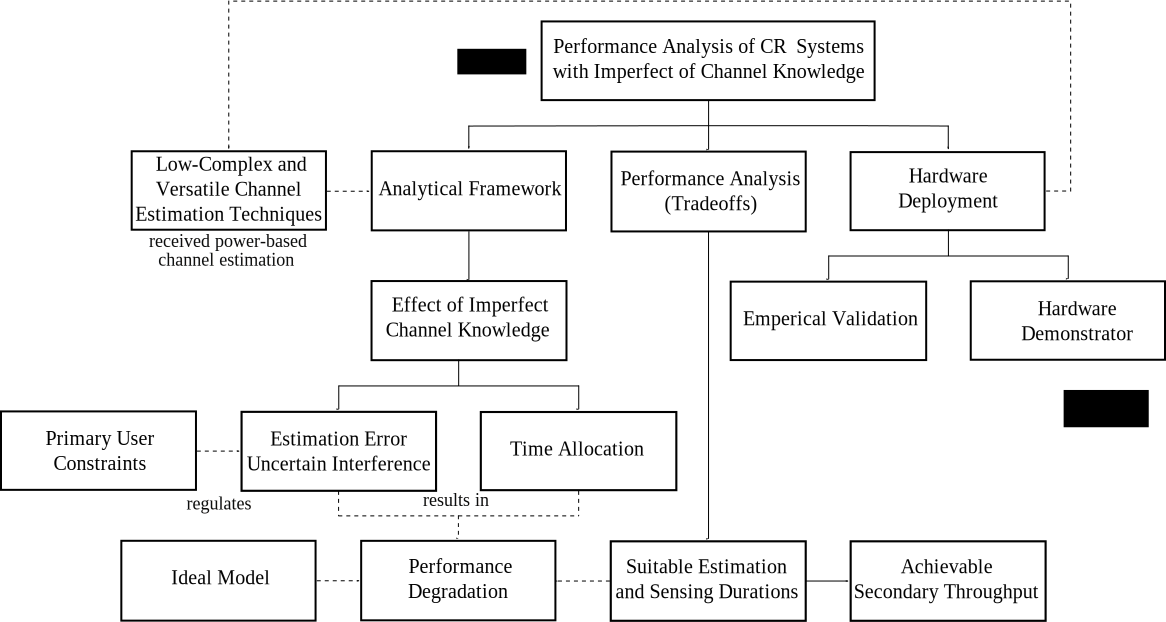
\includegraphics[width=\textheight]{figures/Contri}
        \caption{An illustration of the interconnection between the major contributions and the key observations.}
        \label{fig_Int:contri}
\end{figure}
\else
\begin{sidewaysfigure}
        \centering
        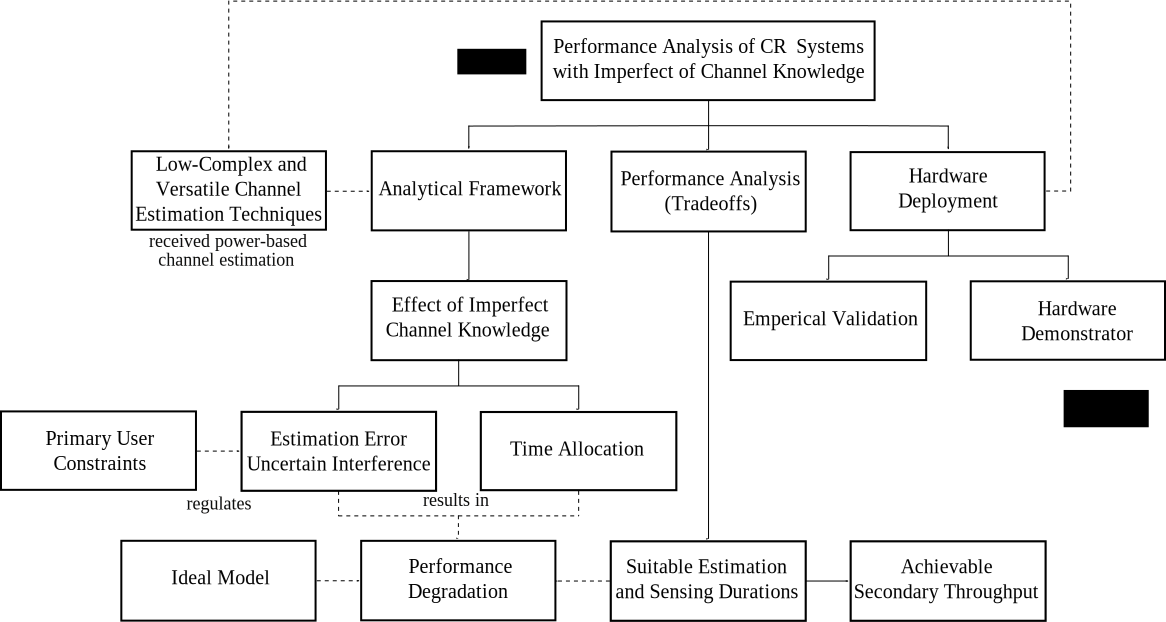
\includegraphics[width=\textheight]{figures/Contri}
        \caption{An illustration of the interconnection between the major contributions and the key observations.}
        \label{fig_Int:contri}
\end{sidewaysfigure}
\fi

\section{Main Contributions}
At this stage, it is well-understood that the knowledge of the related channels is crucial for the application of CR techniques in the practical scenarios. In order to facilitate the hardware deployment of a CSC, a CR application, this thesis capitalizes on the successful integration of this knowledge for different CR systems, namely interweave , underlay and hybrid systems. In this context, the main contributions and the observations of this thesis (highlighted in \figurename~\ref{fig_Int:contri}) are summarized as follows:
\begin{itemize}
\item \textit{Analytical Framework}: 
As a major contribution, this thesis proposes an analytical framework, corresponding to the different CR systems (which are followed in Chapter \ref{chap:IS}, Chapter \ref{chap:US} and Chapter \ref{chap:HS}, respectively) that incorporates the estimation of the involved channels between the primary and the secondary systems, a crucial aspect that has been addressed inadequately in the literature. \begin{mdframed}[style=MyFrame] \textit{Low-complex and versatile channel estimation technique} - In order to satisfy the low complexity and the versatility towards unknown PU signal requirements, which are necessary for the deployment of the CR systems, a received power-based channel estimation is included in the proposed framework.\end{mdframed} \begin{mdframed}[style=MyFrame] \textit{Impact of Incorporating Channel Estimation} - In addition, a careful allocation of the time interval (estimation time), for the purpose of performing channel estimation, in the medium access of the secondary system is proposed. Apart from this, this thesis considers a stochastic approach to tackle the variations in the CR system that arise due to the imperfect channel knowledge (estimation error). In contrast to the existing models that preclude channel estimation (or consider perfect channel knowledge), thereby overestimating the performance of the CR systems, this thesis captures a clear insight on the influence of the time allocation and the imperfect channel knowledge on performance of the CR system. Obviously, the imperfect channel knowledge and the time allocation have an detrimental effect on the performance of the CR system, thus leading to a \textit{performance degradation}. This degradation is qualified through a comparison between the existing models and the estimation model (the one included as a part of the proposed framework). Particularly, the variations cause uncertain interference to the primary system, which in some situations could be deleterious to the primary system, are captured by means of novel constraints introduced as the part of this framework. \end{mdframed} In order to closely examine the relationship between the system parameters, theoretical expressions pertaining to the performance analysis of the CR system are derived. Furthermore, to understand the performance of the proposed framework in fading scenarios, especially the interweave and the underlay systems, the analysis is extended to obtain the theoretical expressions that incur the effect of fading in the involved channels. Finally, to exclude any discrepancy in the analysis, the obtained expressions are validated by means of Monte-Carlo simulations. 
\item \textit{Performance Tradeoffs}: 
As a major observation from the considered analysis, it has been identified that the estimation time is closely associated with the performance of the CR systems. On one side, it is related to the variations incurred in the system, whereby the level of uncertainty in the interference induced due to the channel estimation in the system can be effectively controlled, which ultimately affects the performance in terms of the secondary throughput. While on the other side, the time allocation has a direct influence on the secondary throughput. In this thesis, this kind of dual dependency of the secondary throughput on the estimation time has been investigated in the form of performance tradeoffs, namely \textit{estimation-sensing-throughput} tradeoff for the IS and the HS, and \textit{estimation-throughput} tradeoff for the US. \begin{mdframed}[style=MyFrame] \textit{Suitable estimation and sensing durations} - These tradeoffs present a useful tool for visualizing the response of a CR system (in terms of performance) to different choices of the estimation time so that the performance degradation introduced due to the channel estimation can be carefully regulated. In other words, a system designer can utilize these tradeoffs to preclude situations under which the performance degradation becomes intolerable. Conversely, from a theoretical perspective, these tradeoffs can be used to determine a suitable estimation time that yields the maximum achievable secondary throughput while obeying the interference constraints. \end{mdframed}
 
 
\item \textit{Hardware deployment}: 
In contrast to the theoretical analysis, this thesis lays emphasis on the portability of the analytical framework on a hardware platform. To a great extent, this not only validates the accuracy of the assumptions made while deriving the theoretical expressions but also justifies the applicability of the proposed framework in realistic scenarios. \begin{mdframed}[style=MyFrame] \textit{Empirical Validation} - With the implementation of the received power-based estimation technique, this thesis adds further justification to the claims such as the low complexity and the versatility to unknown PU signals, presented while developing the analytical framework. Considering these facts, a software defined radio platform is deployed for obtaining the measurements required for the validation process. In order to complement the validation, the theoretical expressions, which include the probability density functions that characterize the variations in the estimated parameters and the performance tradeoff are compared with their empirical counterparts. \end{mdframed} \begin{mdframed}[style=MyFrame] \textit{Hardware Demonstration} - Besides validation, this thesis presents a demonstrator that certifies the necessity of channels' knowledge for the performance characterization as-well-as for the operation of a CR system over the hardware. In this regard, following the guidelines of an US, a demonstrator is deployed. \end{mdframed} As a part of the deployment process, % to determine the performance of a CR system. As a major outcome of the deployment process, the significance of the channels' knowledge for the performance characterization as-well-as for the deployment, in context with the CR, is justified. %
in order to illustrate a successful deployment of the CR systems, this thesis identifies and discusses some key issues (the ones which are usually left aside while performing the theoretical analysis) and proposes the corresponding simplifications/solutions.  
\end{itemize}

\section{Organization} %\todo{Reconsider while revising the individual chapters. Also, update the hyper-links to the Sections below.}

The rest of the chapters in this thesis are organized as follows:

Chapter \ref{chap:IS} develops an analytical framework that incorporates the estimation of involved channels in accordance with the interweave scenario. In this context, the indoor deployment scenario is transformed into an interweave scenario, whereby a spectrum sensing mechanism is employed at the CSC-BS enabling a secondary access to the licensed spectrum. Section \ref{sec_IS:ana} derives the theoretical expressions to capture the effect of imperfect channel knowledge on the performance of an IS. Further, Section \ref{sec_IS:num_ana} establishes an estimation-sensing-throughput tradeoff that depicts the suitable estimation and the suitable sensing time at which the maximum secondary throughput is achieved by an IS. 


Following a similar methodology as Chapter \ref{chap:IS}, Chapter \ref{chap:US} develops an analytical framework that incorporates the estimation of involved channels in accordance to the underlay scenario. To implement the underlay technique within the CSC, the deployment scenario is modified such that a power control mechanism is employed at the CSC-BS so that interference remains within the desired tolerance limits at the PR. As a part of the proposed framework, Section \ref{sec_US:th_ana} derives the theoretical expressions for the power control and the secondary throughput, capturing the effect of imperfect channel knowledge and characterizing the performance of an US. In the end, the performance is jointly characterized in terms of estimation-throughput tradeoff that determines the achievable secondary throughput by an US.  

Although the interweave and the underlay system, discussed in Chapter \ref{chap:IS} and Chapter \ref{chap:US}, propose effective ways of performing secondary access, these systems do not represent the best techniques of utilizing the licensed spectrum efficiently. In this regard, to promote the efficient usage of the licensed spectrum by the secondary users, the underlay and the interweave techniques are combined to realize a hybrid scenario. Motivated by this fact, Chapter \ref{chap:HS} develops an analytical framework that incorporates the estimation of involved channels with respect to the hybrid scenario. In this context, the indoor scenario is modified such that the CSC-BS employs spectrum sensing as-well-as power control mechanism to perform secondary access to the licensed spectrum. The theoretical expressions derived in this chapter incorporate the effect of imperfect channel knowledge, depicting the performance of the HS. Analog to Chapter \ref{chap:IS}, an estimation-sensing-throughput tradeoff that yields the achievable secondary throughput for an HS is characterized in this chapter. 

 
In order to reveal the ground truth regarding the analysis proposed in previous chapters, Chapter \ref{chap:HVD} takes into account the deployment aspects of the proposed framework. In this regard, a hardware is deployed that implements the channel estimation, realizes the interference constraints, validates the performance analysis and demonstrates the principle working of the US.   

Finally, Chapter \ref{chap:Con} summarizes the thesis and presents some extensions for future. 

\chapter{Cognitive Relay}
\label{chap:wav}

\section{Cognitive radio}
\begin{itemize}
\item Mitola's concept
\item Dynamic spectrum access for resolving spectrum scarcity
\item Portability using software defined radio
\end{itemize}

\section{Paradigms for Cognitive Radio}
\subsection{Interweave Systems}
\subsection{Underlay Systems}
\subsection{Overlay Systems}

\section{Overview of small cell deployment}
\begin{itemize}
\item Capacity improvements -- femto cell base station -- frequency reuse -- interference coordination 
\item Coverage improvements -- relay -- transparent to the network
\end{itemize}

\section{Cognitive relay as cognitive radio}
\todo{Use case}
Cognitive relay is a network element that provides secondary usage of the spectrum to the devices operating indoor.
\begin{itemize}
\item Capacity improvements through reusing the primary user spectrum
\item Coverage improvements through indoor deployment
\end{itemize}

%\section{Introduction}

%The hardware for radio devices changed dramatically in the last decades and so did the development of waveforms. In former times, waveform development consisted mainly of designing electronic circuits for specific waveforms. Nowadays, waveform development means programming on different processing units like \acp{GPP}, \acp{DSP} or \acp{FPGA}. In addition the way of programming changed from a platform specific to a platform independent development. These approaches deal with a trade-off between efficient platform specific code on the one hand and a portable platform independent code on the other. This chapter gives an overview of the existing and common ways for waveform development and describes in more detail a new approach of the model-based waveform development under the aspect of portability. It furthermore gives a closer look into the performance overhead of generated code by measuring the processing time as well as the logic resources and compares it with hand-written code.

%\section{Use Case}

%\subsection{Platform Specific Development}

%Implementing applications for a specific SDR platform is the traditional way of waveform development. The code is optimized for the underlying processing element and the platform specific tools are used to maximize performance in sense of speed, size and power. Although this is a high-performance approach, existing optimized codes can hardly be ported to other processing elements. If you additionally think of porting the code from \ac{GPP} to \ac{FPGA} this means a complete rewriting of the algorithms.

%\subsubsection{Code Development on Processors}
%For processors, a lot of programming languages exist, but only a few are used for digital signal processing  and embedded systems. This is due to the performance constraints in power, speed and code size. Benchmarks show that C and C++ belong to the most powerful languages in that field \cite{prechelt_comparison}, \cite{language_bench}. However, it has to be mentioned that benchmarks for dedicated programming languages have only limited significance. This is due to the fact that benchmarks for processing times or cycles measure not the language itself but the application behind. Nevertheless, C and C++ are, according to the results from \cite{prechelt_comparison} and \cite{language_bench}, the choices of the \ac{DSP} industry. Figure \ref{fig:dsp_market_share} shows the DSP vendor market shares in 2006. It is remarkable that development environments from these vendors only support C based and assembly languages. According to this result, this work focuses only on C, C++ and optimized libraries written in Assembler.

\begin{figure}[htb]
	\centering
		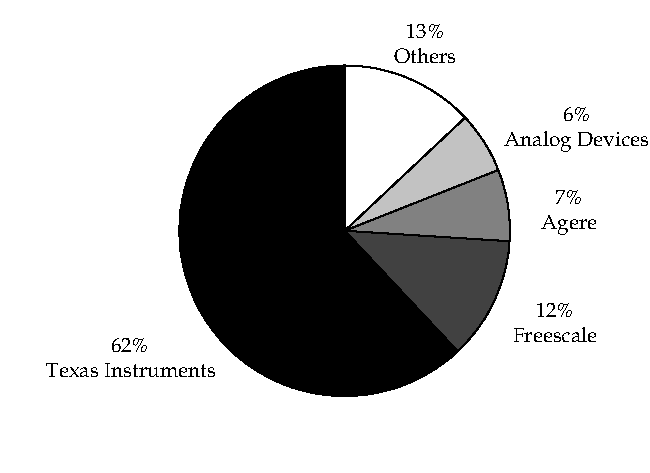
\includegraphics[scale = 0.95]{../kapitel02/figures/dsp_market_share.pdf}
	\caption{DSP vendor market shares in 2006 \cite{strauss_dsp_market}}
	\label{fig:dsp_market_share}
\end{figure}

%Furthermore, a still recent topic is the choice between the languages C, C++ and assembly. The big advantage and the main reason why assembly languages are still used is the direct mapping from language to processor instruction. This mapping gives the programmer any control to optimize the code in the sense of speed and size. Even if the performance constraints are relaxed, small execution times lead to a decrease of the clock frequency and to a lower power consumption. Nevertheless, high-level languages\index{High-Level Language} like C became more and more popular in embedded systems due to three main reasons \cite{dsp_high_level}:
%
%\begin{itemize}
%	\item better portability between hardware platforms
%	\item protection of the investment in program code
%	\item reduced development time
%\end{itemize}
%
%In modern systems, there has to be a trade-off between high-level and low-level programming languages. On the one hand the application should be executed as fast as possible while on the other hand the shrinking time to market calls for portable code. Therefore, almost any vendor for integrated development environments provides user guides and tutorials for C optimizations ( \cite{anderson_optimizing_C}, \cite{ti_opt_C} or \cite{amd_opt_C}). They also claim that well written, efficient and platform independent C code is appropriate for most applications due to platform optimized compilers. The code section represented in listing \ref{source_01} calculates the dot product for two variables in simple C. Listing \ref{unopt_ass_01} shows the assembly code that is produced by the compiler without \index{Optimization}optimizations. By enabling the compiler optimizations, the code is reduced to only a few lines, shown in listing \ref{opt_ass_01}. Due to the fact that the code is written clearly, the compiler is able to optimize it and to use the platform specific architecture. It can calculate two \ac{MAc} operations and simultaneously load two data elements in one single cycle. This example was written for Analog Devices Blackfin DSP and compiled with VisualDSP++.
%
%
%\begin{lstlisting}[columns=flexible,caption=Example code in C,label=source_01]
%for (i=0; i< 150; i++){
%  dotp += b[i] * a[i];
%  sqr  += b[i] * b[i];
%  }
%\end{lstlisting}
%
%\pagebreak
%
%\begin{lstlisting}[caption = Unoptimized assembler code,abovecaptionskip = 0mm,belowcaptionskip = -5mm, label=unopt_ass_01]
%\end{lstlisting}
%\begin{multicols}{2}
%\begin{lstlisting}[columns=flexible]
%[FP+ -8] = R7;
%._ P1L1:
%  R3 = [FP+ -8];
%  R2 = 150 (X);
%  CC = R3 < R2;
%  IF !CC JUMP ._P1L3;
%  R3 <<= 1;
%  P2 = R3;
%  P0 = [FP+ 8];
%  P0 = P0 + P2;
%  R1 = W[P0+ 0] (X);
%  R0 = [FP+ -8];
%  R0 <<= 1;
%  P1 = R0;
%  P2 = [FP+ 12];
%  P2 = P2 + P1;
%  R7 = W[P2+ 0] (X);
%  R7 *= R1;
%  R1 = [FP+ -4];
%  R0 = R1 + R7;
%  [FP+ -4] = R0;
%  R3 = [FP+ -8];
%  R3 <<= 1;
%  P0 = R3;
%  P1 = [FP+ 12];
%  P1 = P1 + P0;
%  R1 = W[P1+ 0] (X);
%  R7 = [FP+ -8];
%  R7 <<= 1;
%  P2 = R7;
%  P1 = [FP+ 12];
%  P1 = P1 + P2;
%  R3 = W[P1+ 0] (X);
%  R3 *= R1;
%  R1 = [FP+ 16];
%  R7 = R1 + R3;
%  [FP+ 16] = R7;
%  R3 = [FP+ -8];
%  R3 += 1;
%  [FP+ -8] = R3;
%  JUMP ._P1L1;
%\end{lstlisting}
%\end{multicols}
%
%\begin{lstlisting}[caption=Optimized assembler code,label=opt_ass_01]
%LSETUP (._P1L2 , ._P1L3-8) LC0=P1;
%._P1L2:
%  A1+= R0.H*R0.H, A0+= R0.L*R0.H (IS)
%      || R0.L = W[I1++]
%      || R0.H = W[I0++];
%			
%._P1L3:
%\end{lstlisting}
%
%There are several other ways of optimizing C code beside the optimizing abilities of the compiler. However, \cite{lee_opt_C} claims that even an optimum assembler code is merely \SI{10}{\%} faster than a well written C code. In addition the rising speed of processors made it possible to pass by the assembly language in most cases. If the code is still too slow, despite of being well written, the positive impact of the Pareto Principle\index{Pareto Principle} can be applied. It says that small code portions (\SI{10}{\%} - \SI{20}{\%}) are consuming most (\SI{80}{\%} - \SI{90}{\%}) of the system resources \cite{pareto}. The performance critical code segments can be identified easily and tuned with optimized assembler code. This can be done for example by applying vectorization or parallelization of the underlying processor. However, these code segments can hardly be ported to other platforms.
%
%A similar discussion about the choice between C and assembly language can be observed in the choice between C and C++. C++ is often seen as slow, inefficient and too large for embedded systems. However, these are assumptions that must not be true, due to the fact that obviously C++ is just a superset of the C language. This means that implementing in C and compiling with a C++ compiler should not produce any overhead. Unfortunately that is not really true. In \cite{dsp_high_level} this overhead was investigated by compiling C benchmark programs with the TASKING DSP563xx C and C++ compilers and comparing the speed and size. The result was that the execution speed decreased by no more than \SI{1.6}{\%} while the code size growed by no more than \SI{6.8}{\%}. C++ features are not consuming much more space than elements in C do if they are well designed. The key issue for writing efficient high-level code (independent of C or C++) is that the developer is aware of the functionality at machine code level and the work of the compiler.
%
%\subsubsection{Code Development on \acp{FPGA}}
%An \ac{FPGA}\index{FPGA} has to be programmed different from a microprocessor or \ac{DSP}, due to its underlying hardware structure (see section \ref{sec:dsp_sdr}). While processors are implemented in assembly language, which can be mapped to the binary machine code instructions, the \ac{FPGA} and its underlying logic is represented by an \ac{HDL}. The \ac{HDL}\index{HDL} is a formal description of the digital logic with reference to the timing behavior. In the beginnings of \acp{HDL} only representations for either the logical behavior or the structure existed. This changed in the 1980s when two new languages appeared, representing the logical and structural behavior: Verilog and VHDL. These languages are still dominating the FPGA world, but their distribution is locally different. While Verilog\index{Verilog} is the most popular \ac{HDL} at the US west coast and Asia, VHDL\index{VHDL} is the preferred language in Europe and the US east coast \cite{baese}. There are various discussions about the advantages and disadvantages of these two \acp{HDL} and several papers compare them based on example applications \cite{verilog_vs_vhdl01}, \cite{verilog_vs_vhdl_02}. The choice between Verilog and VHDL depends lastly not on technical capabilities but on personal references, tool capability and existing code to reuse. 
%
%\subsubsection{Portability with platform specific development}
%Platform specific waveform development is, as indicated by the name, dependent on the underlying processing element. C and C++ code can be ported from one GPP to another without a major decrease in performance. But this is only true under the condition that the operating systems are not changing. The porting of DSP code depends on the underlying architecture. The port from a floating point processor to a fixed point processor forces the compiler to translate every floating point instruction into fixed point instructions with exception handling in case of overflows. Furthermore, a program with processor specific intrinsics can not be ported to a new platform. The sections of the code with the platform specific commands have to be rewritten. Although C and C++ are high level programming languages, there is no assurance that they can be ported without modifications or loss in performance. This is even more dramatic when porting \ac{HDL}. The choice of language is predetermined by the platform developer and provider of the board support kit. Therefore, a specific language has to be used and code can not be ported if it is available in the wrong language.
%
%\subsection{GNU Radio}
%\label{GNURadio}
%\index{GNU Radio}
%
%GNU Radio is an open source project for building waveforms for software defined radios \cite{gnu_radio_art}. The idea is the interpretation of a waveform as multiple components that are composed together. The components with an input and output port build the signal processing blocks, while blocks with only input or output ports can be named sinks or sources. Therefore, the GNU Radio library supports hundreds of components written in C++. The connection between blocks and the creation of waveforms is accomplished by building a flow graph in Python that holds the components as primitives. The code example \ref{gnuradio_01} works as an ``Hello World'' tutorial for GNU Radio. It generates two sine waves with a frequency of \SI{350}{Hz} and \SI{400}{Hz}, adds them and passes the output to the sound card. In lines 13 to 16 the components are defined and configured. The simplicity of GNU Radio can be seen on line 18 and 19. The components can be connected with the instruction \texttt{connect()}. The whole scheduling and necessary inter-process communication is done by GNU Radio itself. 
%
%\begin{lstlisting}[language=Python,columns=flexible,caption=Dial tone example in GNU Radio,label=gnuradio_01]
%#!/usr/bin/env python
% 
%from gnuradio import gr
%from gnuradio import audio
%
%class my_top_block(gr.top_block):
%  def __init__(self):
%    gr.top_block.__init__(self)
%
%    sample_rate = 32000
%    ampl = 0.1
%
%    src0 = gr.sig_source_f(sample_rate, gr.GR_SIN_WAVE, 350, ampl)
%    src1 = gr.sig_source_f(sample_rate, gr.GR_SIN_WAVE, 440, ampl)
%    add  = gr.add_ff()
%    dst  = audio.sink (sample_rate, "")
%        
%    self.connect (src0, (add,0))
%    self.connect (src1, (add,1))
%    self.connect (add, dst)
%
%if __name__ == '__main__':
%  try:
%    my_top_block().run()
%  except KeyboardInterrupt:
%    pass        
%\end{lstlisting}
%
%Despite the comprehensive signal processing library, GNU Radio was only used by few developers through the beginning years. In 2004 Ettus Research LLC released the first version of the USRP as an RF front end that can be connected directly with GNU Radio. Therefore, the community of developers for GNU Radio increased. The next step in the evolution of GNU Radio was the development of a tool, named as \ac{GRC}\index{GRC}, which graphically connects and configures components to a flow graph. The equivalent example from listing \ref{gnuradio_01} is shown in the \ac{GRC} environment in figure \ref{fig:gnuradio_grc}. The graphical flow graph can automatically generate the Python code where lower programming experience for SDR developers is demanded. 
%
%\begin{figure}[htbp]
%	\centering
%		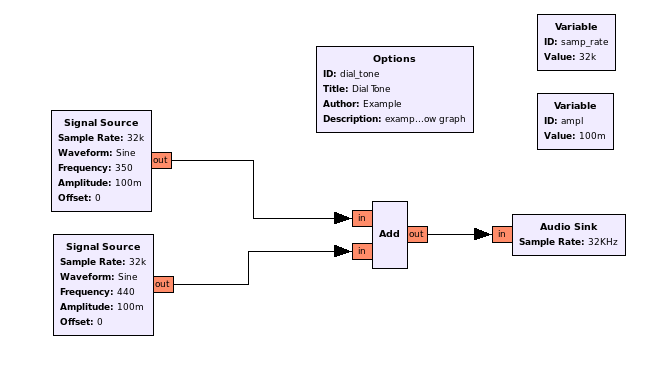
\includegraphics[width=1.00\textwidth]{../kapitel02/figures/gnuradio_grc.png}
%	\caption{Dial tone example in the GNU Radio Companion}
%	\label{fig:gnuradio_grc}
%\end{figure}
%
%GNU Radio composes the waveform with a flow graph and allows the developer to build waveforms that are independent of the underlying hardware. Nevertheless they are not independent of the underlying operating system. In simple terms GNU Radio waveforms are portable between processors that run Linux operating systems. It has to be mentioned that ports of GNU Radio were only successful from a GPP to another GPP. Even if there have been ports to various hardware platforms like Sony's Playstation 3 \cite{gnu_radio_web} and the BeagleBoard \cite{open_sdr}, it has to be mentioned that GNU Radio only ran on the GPP part of these multi core platforms, neither on DSPs nor on FPGAs.
%
%
%\subsection{Software Communication Architecture}
%\label{sec:SCA}
%
%\subsubsection{History of the Software Communication Architecture}
%Waveform development and portability aspects are also enforced by U.S. military. It maintains hundreds of different legacy radios, which are neither upgradeable nor compatible to each other. In parallel the processor capabilities increased in the last two decades according to Moore's Law \cite{moores_law}, \cite{moores_law_2}. This claims that the number of transistors that can be placed on the same area is doubled every other year. The development in chip technology and in the DSP capability resulted in a shift of the borders between analog and digital domain of a radio towards the antenna as mentioned in section \ref{sec:mot}. Therefore, the \ac{JTRS} \ac{JPO} was founded in 1997 to develop a family of the next generation of reconfigurable software-based tactical radios. This system should increase the flexibility and interoperability among the legacy radio systems to reduce the costs for maintenance and to supply and provide the ability to upgrade not only hardware parts but also the software of the radio. The first milestone in this effort was the definition of a common software architecture for these radios: The \ac{SCA}\index{SCA}. To accomplish the \ac{JTRS} project goals, the SCA was intended to support portability between SCA compliant implementations, and to use already established frameworks and architectures from the industry. This should result in minimizing the development time due to reuse of waveform components.
%
%\subsubsection{Operating Environment}
%\index{Operating Environment}
%The \ac{OE} builds the interface between a waveform component and the radio \cite{SCA_Tutorial_VT}. One part of it is the operating system of the radio. To be independent of the underlying hardware and the operating system, the \ac{OE} provides several interfaces for the waveform components to communicate with its environment: These are the interfaces provided by the \acl{CF} and CORBA\index{CORBA} and additionally the \ac{AEP}\index{AEP}. The access points for the application to the operating system are shown in figure \ref{fig:OE}.
%
%\begin{figure}
%	\centering
%		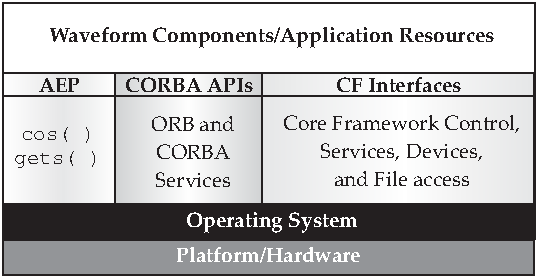
\includegraphics[]{../kapitel02/figures/operating_environment.pdf}
%	\caption{Operating Environment with the connections to the platform and the waveform}
%	\label{fig:OE}
%\end{figure}
%
%\subsubsection{Core Framework}
%\index{Core Framework}
%
%The \ac{CF} provides interfaces to the operating system, which can be used by the waveform or other applications running on the \ac{OE}. The interfaces give access to various services like the installation, management or configuration of a waveform. Another purpose of the interfaces is to abstract the underlying hardware. Therefore, four classes of \ac{CF} interfaces are specified:
%
%\begin{itemize}
%	\item Base Application Interfaces
%	\item Base Device Interfaces
%	\item Framework Control Interfaces
%	\item Framework Service Interfaces
%\end{itemize}
%
%The base application interfaces provide access to waveform components like initializing or releasing, configuring or querying the properties of the different components for testing purposes. The software components for access to the hardware resources are called devices, where the basic device interfaces allow interaction with the physical hardware devices on the radio. The framework control interfaces provide a radio wide control of services like installation, deployment or management while the framework service interfaces supply additional services like management of file systems.
%
%\subsubsection{CORBA}
%\index{CORBA}
%
%The \ac{CORBA} is an open specification for mechanisms calling objects from other processes per remote. The specific characteristic of \ac{CORBA} is, that these objects can run under different operating systems or on different processor architectures and that they can even be implemented with a different programming language. The remote calls can not be distinguished in the implementation from local calls. This is the main reason of the inclusion of \ac{CORBA} in the \ac{SCA} due to the fact that waveform components should exchange information without knowledge of the underlying operating systems and transport mechanisms. Nevertheless, \ac{CORBA} has also some technical restrictions. The most important is the complexity and the size of its \acp{API}, which are quite larger than necessary \cite{rise_fall_corba} and therefore not well suited to an embedded system. To circumvent this, the \ac{SCA} dictates the use of minimumCORBA, standardized by the \acl{OMG}. MinimumCORBA is a subset of \ac{CORBA} designed for systems with limited resources.
%
%\subsubsection{Application Environment Profile}
%\index{AEP}
%
%The \ac{IEEE} and The Open Group specified \acp{API} between application and operating system under the name \ac{POSIX}. The \ac{SCA} \cite{SCA222} dictates with the \ac{AEP} a subset of \ac{POSIX} with 256 \acp{API}. This includes for example mathematical operations like \lstinline[language=C]!cos()!, \lstinline[language=C]!sin()!, \lstinline[language=C]!tan()! or string operations like \lstinline[language=C]!gets()!, \lstinline[language=C]!getchar()!. Due to the fact that these interfaces are standardized, the access from the waveform component to the underlying operating system, is portable without the use of the \ac{CF} or \ac{CORBA}.
%
%
%\subsubsection{Domain Profile}
%\index{Domain Profile}
%
%Beside the aspect of portability, an additional requirement of SCA compliant radios is the reconfigurability. Therefore, the Domain Profile provides an essential description of the platform and the waveform application. The Domain Profile consists of several description files written in \ac{XML}. These files describe:
%\begin{itemize}
%	\item the various hardware devices
%	\item the waveform components
%	\item the deployment
%	\item the connections between components
%	\item the properties of components and devices 
%\end{itemize}
%
%With this information the SCA-compliant radio is able to deploy a waveform, independent of the underlying hardware.
%
%\subsubsection{SCA-compliant waveform development}
%The development of an SCA-compliant waveform requires a good understanding of the \ac{SCA} \ac{CF}. However, there are tools that make it easier for waveform developers. Beside professional tools like SCARI \cite{scari:website}, Spectra \cite{spectra:website} or Component Enabler \cite{ce:website}, the Open Source project Ossie \cite{ossie:website} builds a complete SCA framework with code generation. It already supports interfaces to the USRP and the USRP2 and was ported to environments including FPGAs \cite{ossie_fpga} and DSPs \cite{ossie_omap}. 
%
%\section{Model-Based Development}
%\label{sec:mbd}
%
%\subsection{OMG's Model Driven Architecture}
%\index{MDA}
%The \ac{OMG} is a non-profit international computer industry consortium for standardizing distributed object-oriented software systems as well as model-based developments. It created the development and the standardization of modeling architectures like the Unified Model Language (UML) as well as middleware solutions like \ac{CORBA}, which is described in section \ref{sec:SCA}. In 2001 \ac{OMG} adopted the \ac{MDA}, which can be seen as an approach for the usage of models in software development to provide portability, interoperability and reusability \cite{MDAGuide}. These goals can be achieved by the concept of separating the functionality of an application from the capabilities of the underlying platform. The fundamental idea is to initiate an iterative process in developing models of a specific system and to extend these models in a last step to an application running on a platform. Therefore, the MDA suggests to start the development with a \ac{CIM}\index{CIM} for the requirements of the system, but which is independent of the way how the system is built. The first step of an implementation is the \ac{PIM}\index{PIM}. This is a model that describes the system but does not show details of its use of any platform. The first implementation with platform details is realized in the \ac{PSM}\index{PSM}. As the name implies, this illustrates how the system uses the underlying platform to fulfill the functionality and the requirements specified in the \ac{CIM}. The step from one model to another is called transformation. The \ac{MDA} does not define a specific method for the transformation. However, it gives examples from all manual transformations up to fully automated transformations \cite{MDAGuide}.
%
%In contrast to the \ac{MDA}, the \ac{SCA} is also defining its waveforms in a platform independent manner but models the platform itself in a Platform Specific Model with the Domain Profile. The transformation for this \ac{PSM} to executable code running in real-time on the SDR platform should be done with the Core Framework and \ac{CORBA}. However, \ac{CORBA} comes with overhead in processing time and memory usage and is therefore not the best choice for the baseband processing. Due to this, the MDA should be reinterpreted to fit the needs of baseband processing on heterogeneous hardware architectures.
%
%\subsection{A new interpretation of the MDA} 
%The introduced models \ac{CIM}, \ac{PIM}, and \ac{PSM} build the basis of the \ac{MDA} and should should be maintained. However, the interpretation should be more application specific concerning the air interface. The \ac{CIM} that should describe the requirements independent of the implementation is actually the specification of the waveform. While most specifications for industry waveforms are open to public (e.g. specifications of \ac{IEEE} or \ac{ETSI}), this is not the case for military waveforms. These waveforms were built for legacy devices where the baseband data were processed with hardware. The specifications are not open and in some cases not even existent. This results in a lot of work for reengineering and creating the \ac{CIM} when the waveform should be supported by an SDR. The transformation to the \ac{PIM} can be accomplished by implementing the waveform without platform specific aspects. Therefore high-level languages can be used, which support good debug and simulation features. The \ac{PIM} is a model for the implementation of the waveform's functionality. This includes for example the realization of the synchronization schemes or the design of the digital filters. The step to the \ac{PSM} is done by extending the \ac{PIM} with platform specific aspects. These can be infrastructural platform aspects like the data buses on the system or the configuration of the RF front ends and \acp{ADC}. Further platform specific aspects are processor specific issues like the adaption of algorithms for fixed-point representations. The last transformation from the \ac{PSM} to an executable code is done automatically with code generation tools like \emph{Real Time Workshop} or \emph{HDL Coder} from the company The Mathworks and processor specific compilers like \emph{Visual C Compiler} from Microsoft, \emph{Code Composer Studio Compiler} from \ac{TI} or \emph{Intel Parallel Studio}. Another example for this use of the \ac{MDA} is described in \cite{schober_mda} and \cite{nagel_tetra}. Figure \ref{fig:mda_structure} summarizes the steps from CIM to Code.
%\begin{figure}
%	\centering
%		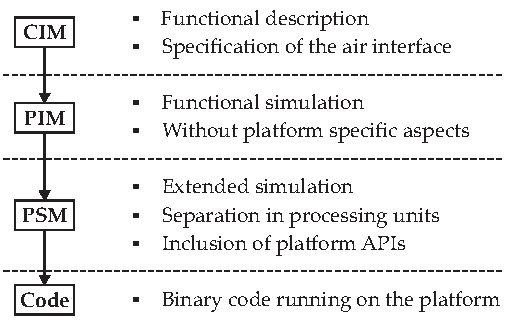
\includegraphics[]{../kapitel02/figures/mda_structure.pdf}
%	\caption{Overview of the models, which are defined by the MDA}
%	\label{fig:mda_structure}
%\end{figure}
%
%
%
%\subsection{Model-Based Design with Simulink}
%\index{Simulink}
%Simulink \cite{simu_ug} is a visual programming language, which allows engineers to model dynamic systems. It provides hundreds of blocks, which generate, process and consume data. Furthermore, Simulink supports extensions to generate code in the languages C, C++, Verilog and VHDL. It is therefore used in this work for waveform development. This section should give an overview of the principles of Simulink and its extensions to code generation.
%
%\subsubsection{Simulation}
%In introductions to programming languages the ``Hello World'' example is used very often. However, this does not make sense for a visual programming language that is used for digital signal processing. A better example is the ``dial tone'' example from section \ref{GNURadio}. The generation and processing of two sine waves gives an overview of the necessary parameters and configurations.
%
%
%\begin{figure}
%	\centering
%		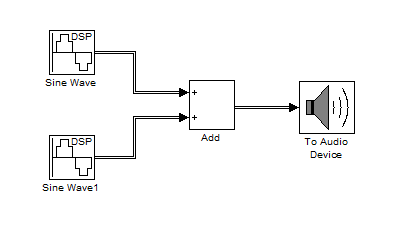
\includegraphics[width=0.75\textwidth]{../kapitel02/figures/dial_tone_simu.PNG}
%		\caption{Dial tone example in Simulink}
%	\label{fig:dial_tone_simu}
%\end{figure}
%
%Figure \ref{fig:dial_tone_simu} shows the dial tone example in a Simulink environment. The blocks require information about the sample time as well as frequency and magnitude of both sine waves. This does not differ from the \ac{GRC} model described in section \ref{GNURadio}. The difference is in the optional handling of the data. While GNU Radio considers the data flow as a stream without the knowledge of the actual processing, Simulink provides the opportunity to parameterize the size of vectors in the initialization phase. This results in new degrees of freedom. While the processing on single values (sample-based)\index{Sample-based processing} minimizes latency, the throughput is decreased due to the \ac{ISR} after each sample. Working on multiple values (frame-based)\index{Frame-based processing} increases the latency and the memory usage but optimizes the performance with respect to execution time. Figure \ref{fig:sample_frame} clarifies this relation.
%
%\begin{figure}
%	\centering
%		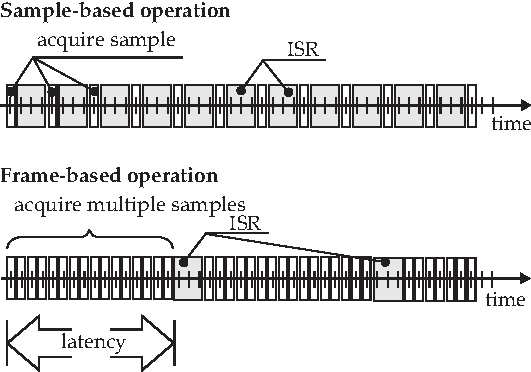
\includegraphics{../kapitel02/figures/sample_frame.pdf}
%	\caption{Comparison of latency and throughput for sample-based and frame-based processing}
%	\label{fig:sample_frame}
%\end{figure}
%
%
%\subsubsection{Code Generation from Simulink to C/C++}
%\label{sec:codegen}
%Real Time Workshop \cite{rtw_ug} and Real Time Workshop Embedded Coder \cite{rtwec_ug} extend Simulink's functionalities with the ability to generate C and C++ code for real-time systems. For building executable models, it is not only necessary to generate the code for the algorithmic function. This code must also support run time interfaces as well as scheduler and memory transfer. Therefore, the following steps are executed:
%
%\begin{itemize}
%	\item \textbf{\texttt{ModelInitialize}}: Initializes the code for the run-time interface and the model. This includes  allocation of memory and data that can be calculated prior to the execution of the algorithm.
%	\item \textbf{\texttt{ModelOutput}:} Calls all blocks in the model that have a sample hit at the current time and 
%	produce their output. The output follows a given simulation time step.
%	\item \textbf{\texttt{ModelUpdate}:} Calls all blocks in the model that have a sample hit at the current point in time and update their discrete states.
%	\item \textbf{\texttt{ModelTerminate}:} Terminates the program if it is designed to run for a finite time. It deallocates memory and can write data to a file.
%\end{itemize}
%
%The pseudo code in listing \ref{rtw_01} shows how these functions are integrated in the generated code. 
%
%\begin{lstlisting}[language=C,columns=flexible,caption= Structure of a generated model in pseudo code \cite{rtw_ug},label=rtw_01]
%rtOneStep()
%{
%  //Check for interrupt overflow
%  //Enable "rt_OneStep" interrupt
%  ModelOutputs();    // Major time step.
%  LogTXY();          // Log time, states and root outports.
%  ModelUpdate();     // Major time step. 
%}
%
%main()
%{
%  ModelInitialize();
%  //including installation of rtOneStep as an 
%  //interrupt service routine for a real-time clock
%  
%  while(time < final time){
%  	rt_OneStep();
%    //Background task
%    }
%  ModelTerminate();
%  //Mask interrupts (Disable rt_OneStep() from executing.)
%  //Complete any background tasks.
%  //Shutdown
%}     
%\end{lstlisting}
%
%The C++ code from the dial tone example shown in figure \ref{fig:dial_tone_simu} was generated for a better overview of these functions working with a model. Listing \ref{rtw_02} shows the initialization of this configuration with the step size according to the sample rate of \SI{32}{kHz} and the memory allocation of the block input and output arrays.
%
%\begin{lstlisting}[language=C,columns=flexible,caption= Initialization of the model,label=rtw_02]
%dial_tone_initialize(){
%  dial_tone_M->Timing.stepSize = (0.032);
%  dial_tone_M->ModelData.blockIO = ((void *) &dial_tone_B);
%  (void) memset(((void *) &dial_tone_B), 0,
%                sizeof(BlockIO_dial_tone));
%  ...
%  }
%\end{lstlisting}
%
%In listing \ref{rtw_03} the actual signal processing is shown for the \texttt{ModelOutput} function, which is in this case the addition of two sine waves with a frame length of 1024 as the iteration size for the loop.
%  
%\begin{lstlisting}[language=C,columns=flexible,caption= Signal processing in the dial tone,label=rtw_03]
%dial_tone_output(){
%  ...
%  for (i = 0; i < 1024; i++) {
%    dial_tone_B.Add[i] = dial_tone_B.SineWave[i]
%                       + dial_tone_B.SineWave1[i];
%  }
%  ...
%  }
%\end{lstlisting}
%
%In the code section from the \texttt{dial\_tone\_update} function in listing \ref{rtw_04}, two parameters are shown. The first is the call of the sound card with the memory address of the adders output. The second is the increment of the step size. 
%
%\begin{lstlisting}[language=C,columns=flexible,caption= Update of the model's states,label=rtw_04]
%dial_tone_update(){
%  ...
%  LibUpdate_Audio(
%           &dial_tone_DWork.ToAudioDevice_AudioDeviceLib[0],
%           &dial_tone_B.Add[0], 0, 1024, 0);
%  ++dial_tone_M->Timing.clockTick0;
%  dial_tone_M->Timing.t[0] = dial_tone_M->Timing.clockTick0 *
%                  dial_tone_M->Timing.stepSize0;
%  ...
%  }
%\end{lstlisting}
%
%The models are finalized by terminating the call of the sound card and freeing all memory space as shown in listing \ref{rtw_05}.
%
%\begin{lstlisting}[language=C,columns=flexible,caption= Termination of the model,label=rtw_05]
%dial_tone_terminate(){
%  ...
%  LibTerminate(
%           &dial_tone_DWork.ToAudioDevice_AudioDeviceLib[0]);
%  LibDestroy(
%           &dial_tone_DWork.ToAudioDevice_AudioDeviceLib[0], 1);
%  ...
%	}
%\end{lstlisting}
%
%\subsubsection{Code generation from Simulink to Verilog/VHDL}
%The HDL Coder extension of Simulink \cite{hdl_ug} provides the ability to generate Verilog or VHDL code for a model. This leads, with the support of C code generation and simulation, to a system that is highly capable of building and transforming models for heterogeneous processing platforms. The code generation shall be introduced by the already known dial tone example. However, the output is not connected to a sound card but to an output port for the dedicated module. Some minor changes have to be applied to the model to assure that the code can be generated. Due to the fact that FPGAs do not support floating point arithmetic, the sine waves must be configured to generate fixed point output. In difference to DSPs, FPGAs are not working on arrays. This means that the processing changed to be based on samples. With these changes, HDL code can be generated.
%
%\begin{figure}
%	\centering
%		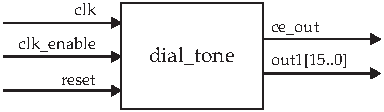
\includegraphics{../kapitel02/figures/dial_tone_fpga.pdf}
%	\caption{Structure of the generated \texttt{dial\_tone} module}
%	\label{fig:dial_tone_fpga}
%\end{figure}
%
%
%\begin{lstlisting}[language=Verilog,columns=flexible,caption= Extraction of the generated Verilog code,label=hdl_01]
%module dial_tone(...)
%
%always @(address_cnt_1)
%  ...
%  begin
%    case(address_cnt_1)
%      7'b0000000 : Sine_Wave1_out1 = 16'b0000000000000000;
%      7'b0000001 : Sine_Wave1_out1 = 16'b0000100000001001;
%      ...
%    endcase
%  end  
%  assign Add_add_cast = Sine_Wave_out1;
%  assign Add_add_cast_1 = Sine_Wave1_out1;
%  assign Add_add_temp = Add_add_cast + Add_add_cast_1;
%  assign Out1 = Add_add_temp[15:0];
%  
%endmodule  // dial_tone
%\end{lstlisting}
%
%Listing \ref{hdl_01} shows an extraction of the generated Verilog code for the dial tone example. The sine waves are generated by a lookup table and the output is assigned to the highest 16 bit of the sum of the sine waves. Figure \ref{fig:dial_tone_fpga} shows the structure of the generated Verilog module.
%
%\section{Overhead of Code Generation}
%\label{sec:overhead}
%
%The efficiency of generated code is still highly controversial in the development of radio systems. While some are complaining about the fact that the code is too slow baseband signal processing, others argue that there is no overhead. In this section, the processing time of the generated code was measured on different processing units under varying conditions like compilers or data types. It is furthermore compared with an unoptimized hand written code and an assembly-based optimized code. Parts of these measurements were also published in \cite{perf_overhead}.
%
%
%\subsection{Code Generation for GPPs}
%
%The benchmarks for generated C/C++ code were executed on an Intel Core 2 Duo CPU (P8400) with a clock frequency of \SI{2.28}{GHz}. The processor is working with a Windows 7 operating system and three compilers:
%\begin{itemize}
%	\item In the following the C/C++ compiler, which is integrated in Visual Studio 2005, is named \emph{VS}. The comparison with newer versions of the Visual Studio Express Edition showed no differences in speed. Therefore only this version is listed in the results.
%	\item The Local C Compiler in the following denoted as \emph{LCC} is a small open source C compiler, where in the benchmarks, version 2.4.1 is used.   
%	\item Intel Parallel Studio XE2011 integrates a C/C++ compiler in the development environment, which is especially suited for Intel architectures. The compiler is subsequently denoted as \emph{IPS}.
%\end{itemize}
%
%The C/C++ code was generated with Real Time Workshop version 7.6. For better readability and comparison with different processors, the benchmarks show, beside the time consumption of the evaluated code, also the number of cycles. These are calculated by the processing time multiplied with the processor frequency. Therefore, it is just a time scaling.
%
%Figure \ref{fig:empty_loop_gpp} shows the overhead that the generated code consumes after every \ac{ISR} due to scheduling, logging and status updates. This is the time the code remains in the gray boxes in figure \ref{fig:sample_frame}. It can be seen that the choice of the compiler dramatically influences the differences in processing times. The \ac{IPS} consumes less than a third of the time than the \ac{LCC}. The figure indicates also the influence of the frame size on the generated overhead. While the processing time of the non-functional code in figure \ref{fig:empty_loop_gpp} remains constant, the processing time for code inside the \texttt{model\_output} function increases with the frame size and leads to a better throughput in total.
%
%\begin{figure}[htbp]
%	\centering
%		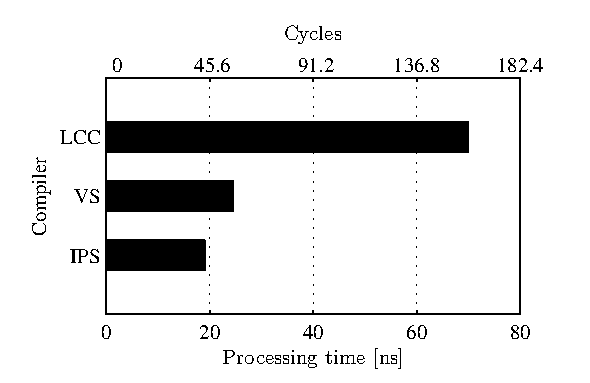
\includegraphics{../kapitel02/figures/empty_loop_gpp.pdf}
%	\caption{Processing times of the generated non-functional code, which was compiled with various compilers}
%	\label{fig:empty_loop_gpp}
%\end{figure}
%
%One of the essential signal processing functions in SDRs are \ac{FIR} filters\index{FIR filter}. Figure \ref{fig:fir_gpp} shows the benchmark of an \ac{FIR} filter compiled with the aforementioned compilers. To present values independent of the number of taps and frame size, the results are normalized to one input sample and one tap, leading in the best case to only one \ac{MAc} operation. Additionally to the named compilers, the data type (real or complex) and the code (hand written or generated) are compared. The results for the compilers from figure \ref{fig:empty_loop_gpp} are also valid for this benchmark. The \ac{VS} and \ac{IPS} produce the fastest code. The generated code consumes always less time than the hand written code. Note that the hand written code is not optimized in any sense except in the implementation of a circular buffer. The source code of the unoptimized hand written FIR filter can be found in appendix \ref{sec:app_FIR}. The fastest code is the generated code for an \ac{FIR} filter with real data and compiled with the \ac{IPS}. Only three cycles are consumed on the GPP per real tap and real sample. The processing time for a complex operation takes about ten cycles, which is also a good result, taking into account that the complex \ac{MAc} operation needs four real multiplications and two additions.
%
%\begin{figure}[htbp]
%	\centering
%		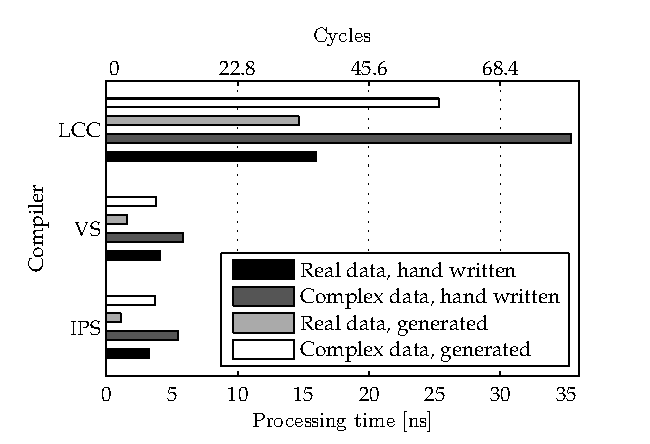
\includegraphics{../kapitel02/figures/fir_gpp.pdf}
%	\caption{Benchmark of an FIR filter on a GPP}
%	\label{fig:fir_gpp}
%\end{figure}
%
%Another important algorithm used in a waveform implementation is the \ac{FFT}\index{FFT}. Figure \ref{fig:fft_gpp} compares the processing times of an \ac{FFT} for \emph{generated code}, \emph{unoptimized hand written code} and an \emph{optimized code}. This optimized code comes from FFTW, which is a C subroutine library for calculating discrete Fourier Transforms. It is supported by an open software platform and is in performance comparable to machine-specific, vendor-optimized codes. The good performance is achieved by querying the parameters through the operating system and tuning the architecture automatically for the fastest results \cite{fftw_paper}. The unoptimized code is the straight implementation of the Cooley-Tukey algorithm, which can be found in appendix \ref{sec:app_03}.
%
%\begin{figure}[htbp]
%	\centering
%		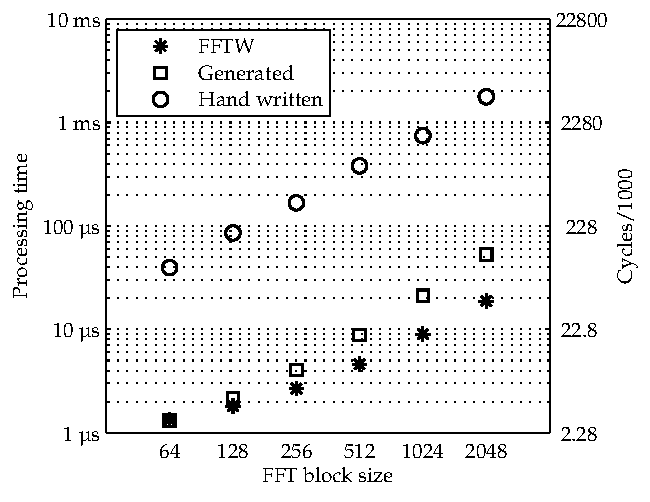
\includegraphics{../kapitel02/figures/fft_gpp.pdf}
%	\caption{Benchmark of the FFT on a GPP}
%	\label{fig:fft_gpp}
%\end{figure}
%
%For better comparability the compiler times are not included in the above results. The differences in the times for the compilers are in accordance to the previous results, which are shown in figure \ref{fig:empty_loop_gpp}. The input data are complex floating point vectors with a length according to a power of two. The hand written code is about thirty times slower than the generated and optimized code. They are varying over the FFT block size according to the benchmarks of the FFTW in \cite{fftw_bench}. There, it is shown, that the FFTW implementation achieves the best speed results with FFT sizes between 512 and 2048. The speed of the generated code does not fully reach the optimized FFTW implementation.
%
%
%
%\subsection{Code Generation for DSPs}
%
%The benchmarks for generated C code were measured with a C64x+ core on Texas Instrument's DM6446 system on chip, which is described in more details in section \ref{sec:SFF}. The processing times and cycles are in accordance with the GPP measurements when taking the scaling factor of the DSP's clock frequency of \SI{594}{MHz} into account. The C code is compiled with \ac{CCS} from the \ac{DSP} vendor \ac{TI}. Figure \ref{fig:empty_loop_dsp} shows an overhead of \SI{3.8}{\micro s} of the generated non-functional code. Referring to the number of cycles, this is about fifty times more than the non-functional code for the GPP. This is mainly caused by the underlying fixed point processor that has to deal with floating point code.
%
%\begin{figure}[htbp]
%	\centering
%		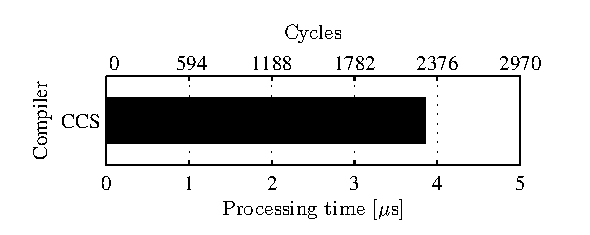
\includegraphics{../kapitel02/figures/empty_loop_dsp.pdf}
%	\caption{Overhead of the non-functional code on a DSP}
%	\label{fig:empty_loop_dsp}
%\end{figure}
%
%The performance loss of floating point code on a fixed point processor can also be seen in the benchmark of an \ac{FIR} filter\index{FIR filter} represented in figure \ref{fig:fir_dsp}. While the difference between floating point and fixed point arithmetic with hand written code makes a factor of ten, the generated fixed point code is about hundred times faster than the generated code dealing with floating point data types. The optimized code with a special library for digital signal processing comes from \ac{TI} and is only available in fixed point arithmetic. The generated fixed point code needs twice the time, which is not a bad result compared with the hand written, non-optimized code.
%
%\begin{figure}[htbp]
%	\centering
%		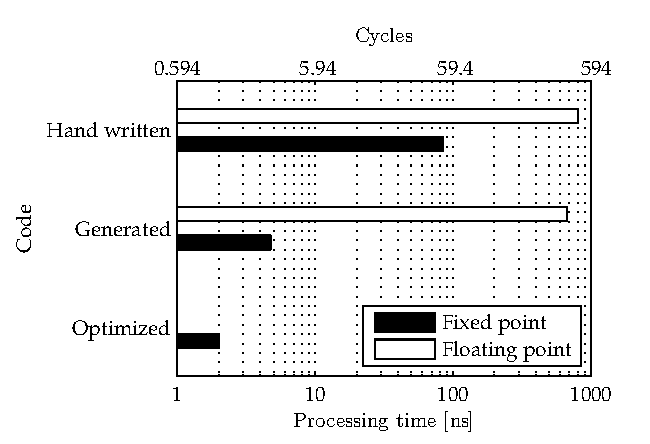
\includegraphics{../kapitel02/figures/fir_dsp.pdf}
%	\caption{Benchmark of an FIR filter on a DSP}
%	\label{fig:fir_dsp}
%\end{figure}
%
%Figure \ref{fig:fft_dsp} compares the results for the \ac{FFT}\index{FFT} for \emph{hand written code}, \emph{generated code} and the \emph{assembler optimized code} from TI's signal processing library. It has to be noted that the hand written code uses floating point arithmetic in contrast to the other code. This leads to the poor results, which are in processing time several decades slower than the optimized codes. The speed up for the optimized code is about four times higher than the generated C code.
%
%\begin{figure}[htbp]
%	\centering
%		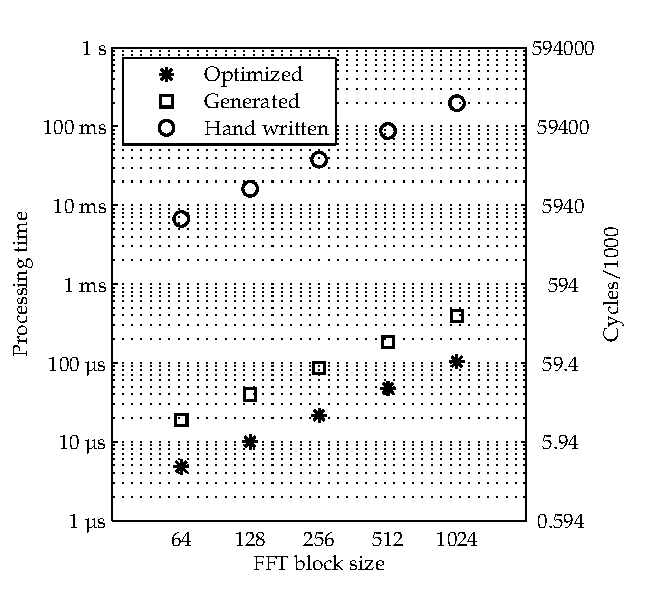
\includegraphics{../kapitel02/figures/fft_dsp.pdf}
%	\caption{Benchmark of the FFT on a DSP}
%	\label{fig:fft_dsp}
%\end{figure}
%
%
%\subsection{Code Generation for FPGAs}
%
%In contrast to the generated codes for \acp{DSP} and \acp{GPP}, the generated \ac{HDL} code creates no overhead for the system. The main task of the \ac{FPGA} on a \ac{SDR} is the adaptation of the DSP sample rate to the higher data rate of the \ac{DAC} and vice versa. Therefore, decimation and interpolation filters have to be realized. Figure \ref{fig:cic_fpga} shows the resource usage of interpolation filters with a \ac{CIC}\index{CIC filter} structure. The filters were implemented on a Virtex 4 FPGA from Xilinx with \acs{VHDL} \cite{virtex4} and on a Cylone FPGA from Altera with Verilog \cite{cyclone2}.
%
%\begin{figure}[htb]
%	\centering
%		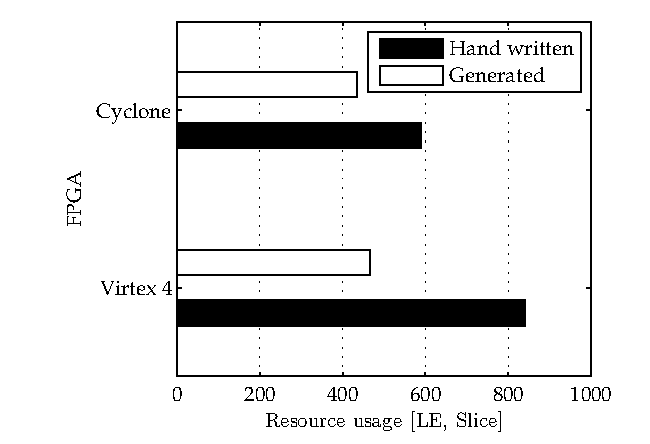
\includegraphics{../kapitel02/figures/cic_fpga.pdf}
%	\caption{Benchmark of a CIC decimation filter on different FPGAs}
%	\label{fig:cic_fpga}
%\end{figure}
%
%The interpolation factor was 128 and the bit lengths for input and output were 16. The bit length inside the filter increased to 44 due to bit pruning. The filter was implemented with four cascaded stages. Due to the different hardware architectures, the resource usage between both FPGAs can not be compared. The FPGAs from the company Altera are based on \ac{LE}\index{Logic Element}, which mainly consists of one programmable register, one carry chain and one \ac{LUT} with four inputs. This is different from the Xilinx approach. The smallest logic block is named ``slice''\index{Slice}, comprising two \acp{LUT} with four inputs, one carry chain and two programmable registers. Therefore, the resource usage of the filter was measured in \acp{LE} for the Cyclone and in slices for the Virtex FPGA. The generated code is smaller in the sense of space than the hand written code but the difference is not as dominating as in the previous sections.
%
%
%Beside \ac{CIC} filters, also \ac{FIR}\index{FIR filter} filters, used for decimation in time, are benchmarked. Figure \ref{fig:fir2_fpga} shows the difference between an optimized halfband decimation filter in comparison to the generated polyphase decimation filter. The filter length was 31 but due to the coefficient properties, only eight multiplications were needed. The other coefficients were zero. Furthermore, due to the symmetry of the filter some coefficients were equal. The generated filter did not recognize this symmetry and hence the possibilities to use this for optimization.
%
%\begin{figure}[htbp]
%	\centering
%		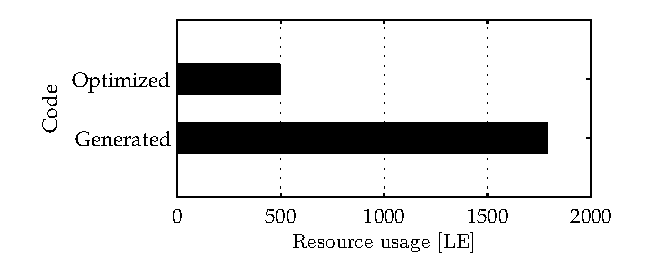
\includegraphics{../kapitel02/figures/fir2_fpga.pdf}
%	\caption{Comparison of the resource usage for a 31-tap halfband filter}
%	\label{fig:fir2_fpga}
%\end{figure}
%
%To get an overview how the number of taps correlate with the resource usage in generated code, Figure \ref{fig:fir_fpga} shows the used \acp{LE} of a decimate by two filter. The bit length of input and output signal as well as the filter coefficients was 16 bit, the bit length of the accumulator was 32 bit. The results of figure \ref{fig:fir_fpga} were measured on a Cyclone FPGA without hardware multipliers.
%
%\begin{figure}[htbp]
%	\centering
%		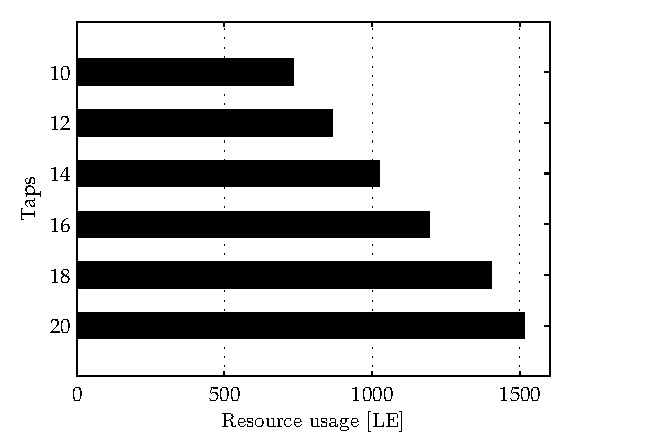
\includegraphics{../kapitel02/figures/fir_fpga.pdf}
%	\caption{Comparison of the resource usage of an FIR decimation filter with various tap lengths}
%	\label{fig:fir_fpga}
%\end{figure}
%
 
\chapter{Interweave System}
\label{chap:IS}
\index{Interweave System}

Secondary access to the licensed spectrum is viable only if the interference is avoided at the primary system. In this regard, different paradi- gms have been conceptualized in the existing literature. Among these, interweave systems (ISs) that employ spectrum sensing have been widely investigated. %This makes performance characterization of a cognitive radio system critical, hence, an interesting research problem. 
Baseline models investigated in the literature characterize the performance of IS in terms of a sensing-throughput tradeoff, however, this characterization assumes the perfect knowledge of the involved channels at the secondary transmitter, which is unavailable in practice. %As a result, these models depict an ideal scenario, thereby making the performance characterization based on these models disputable and impractical for hardware deployment. 
Motivated by this fact, a novel approach that incorporates channel estimation in the system model is established, %, whereby imposes a fundamental limit on the performance of cognitive radio as interweave system. 
%In order to enable secondary access to the licensed spectrum, several paradigms have been conceptualized. Of these, interweave systems that employ spectrum sensing have been widely investigated in the literature. According to which, the interference is avoided by sustaining detection probability above a desired level. Upon satisfying the constraint, the secondary transmitter intends to optimize its throughput. 
%In literature, this optimization has been characterized in terms of sensing-throughput tradeoff. 
%Conventional investigations on the performance of interweave system that employ spectrum sensing at the secondary transmitter have assumed the perfect knowledge of interacting channels. 
%Sensing the energy over the primary user spectrum has been widely investigated in the literature. 
%According to which, an optimum throughput can be achieved by operating at a suitable sensing time. 
%This characterization however considers the knowledge of the channels at the secondary transmitter, this, depicts an ideal scenario. %(primary transmitter - secondary transmitter, secondary transmitter - secondary receiver, primary transmitter - secondary receiver)
%While considering a hardware deployment, this knowledge is essential. Motivated by this fact, we propose a novel system model that incorporates channel estimation. 
 and consequently investigate the impact of imperfect channel knowledge on the performance of the IS. More particularly, the variation induced in the detection probability affects the detector's performance at the secondary transmitter, which may result in severe interference at the primary receivers. In order to capture this variation, an average constraint and an outage constraint on the detection probability is proposed.
%Using these constraints, we characterize the true performance of the IS. 
%Our analysis reveals that the ideal scenario considerably overestimates the performance of the IS. 
The analysis reveals that with an appropriate choice of the estimation time determined by the proposed approach, the degradation in performance of the IS can be effectively controlled, and subsequently the achievable secondary throughput can be significantly enhanced.




%%%%%%%%%%%%%%%%%%%%%%%%%%%%%%%%%%%%%%%%%%%%%%%%%%%%%%%%%%%%%%%%%%%%%%%%%%%%%%%%%%%%%%%%%
%\section{Introduction}
%%%%%%%%%%%%%%%%%%%%%%%%%%%%%%%%%%%%%%%%%%%%%%%%%%%%%%%%%%%%%%%%%%%%%%%%%%%%%%%%%%%%%%%%%
%\subsection{Background}
%Goldsmith \textit{et .al} \cite{Goldsmith09}

\section{Related Work}

In order to enable interference-free access to the licensed spectrum, ISs employ spectrum sensing at the ST. Spectrum sensing (or only sensing) is necessary for detecting the presence or the absence of a primary user (PU) signal. In this way, sensing assists the ISs in protecting the PRs against harmful interference. \tc{A sensing mechanism} at the ST can be accomplished by listening to the signal transmitted by the primary transmitter (PT).
The existing models termed as baseline models investigated in the literature \cite{Liang08, Sharma14, Pradhan15} characterize the performance of IS in terms of a sensing-throughput tradeoff. However, this characterization assumes the perfect knowledge of the involved channels at the ST, which is unavailable in practice. In this regard, a novel approach that incorporates channel estimation in the system model is established, and consequently the impact of imperfect channel knowledge on the performance of the IS is investigated. More particularly, the variation induced in the detection probability affects the detector's performance at the secondary transmitter, which may result in severe interference at the PRs. In order to control the excessive interference, average and outage constraints on the detection probability are proposed. 

For detecting a PU signal, several techniques such as energy detection, matched filtering, cyclostationary and feature-based detection exist \cite{Sharma15, Axell12}. Because of its versatility towards unknown PU signals and its low computational complexity, energy detection has been extensively investigated in the literature \cite{Urkowitz, Kostylev02, Alouini03, Herath09, Mariani10}. In this technique, the decision is accomplished by comparing the power received at the ST to a decision threshold. In reality, the ST encounters variations in the received power due to the existence of thermal noise at the receiver and fading in the channel. Subsequently, these variations lead to sensing errors described as misdetection and false alarm, %The characterization of sensing errors as detection probability and false alarm probability has been studied in \cite{tan08}. 
which limit the performance of the IS. In order to determine the performance of a detector, it is essential to obtain the expressions of detection probability and false alarm probability.

In particular, detection probability is critical for ISs because it protects the PR from the interference induced by the ST. As a result, the ISs have to ensure that they operate above a target detection probability \cite{peh07}. Therefore, the characterization of the detection probability becomes absolutely necessary for the performance analysis of the IS. In this context, Urkowitz \cite{Urkowitz} introduced a probabilistic framework for characterizing the sensing errors, however, the characterization accounts only for the noise in the system. To encounter the variation caused by channel fading, a frame structure has been introduced in \cite{Liang08} \tc{assuming that the channel remains} constant over the frame duration, however, upon exceeding the frame duration, the system may observe a different realization of the channel. \tc{Based on this frame structure, the performance of the IS has been investigated in terms of a deterministic channel \cite{Liang08, Sharma14, Pradhan15} and a random channel\footnote{\tc{In the literature, deterministic and random channels are interpreted as path-loss and fading channels, respectively.}} \cite{Kostylev02, Alouini03, Herath09}. Complementing the analysis in \cite{Liang08, Sharma14, Pradhan15}, the involved channels are considered to be deterministic and random.} 

%The long-term characterization is a classical approach that applies a fading model to average out the variation in the received power. Subject to the deployment scenarios\footnote{These scenarios include urban, suburban and rural, or indoor and outdoor from a different perspective.}, different fading models -- Rice, Rayleigh, Nakagami-$m$ and Log-normal can be employed \cite{Simon00}. The analytical expressions for the expected detection probability for these fading models are characterized in \cite{Kostylev02, Alouini03, Herath09}. Considering a CR system, this approach has some major drawbacks. Fading models depict a long-term characterization of the system, however, short-term or bursty interference that may lead to outage is ignored, thereby deteriorating the performance of a primary system. Moreover, fading models are specific to the deployment scenario, hence, knowledge of the fading model is necessary when designing a CR system. Apart from that, every fading model contains certain model parameters. As a result, estimation of these parameters at the ST \cite{Kaushik14}, particularly during the initial phase of the deployment, imposes an additional overhead on the secondary system. In practice, due to mobility, most systems are likely to violate stationarity over a long duration. Thus, it becomes challenging to track these model parameters. As a consequence, these drawbacks restrict the applicability of this approach to practical CR systems. 

%To overcome the aforementioned drawbacks, an alternative approach that considers the short-term characterization has been established \cite{Liang08, Sharma14, Pradhan15} in such a way that the performance can be analyzed for a single frame\footnote{By a single frame, we refer to the statistical realizations of the received power, whereas \cite{Liang08, Sharma14, Pradhan15} consider the temporal realizations of the same across several frames. Considering ergodic behaviour of the noise, the performance characterization under these two scenarios are equivalent.}. In this way, unlike long-term approach, we preclude the variation due to the channel and consider the variation due to noise in the system. Subsequently, this approach does not need to consider the deployment of the fading model and its complexities thereafter. Motivated by these facts, we focus on the short-term approach for performance analysis.  


Besides the detection probability, false alarm probability has a large influence on the achievable throughput of the secondary system. %Further, the characterization of the false alarm probability requires the knowledge of the noise power. Subject to a given uncertainty \cite{Tan08}, this knowledge can be acquired through hardware calibration. 
%\subsection{Problem Formulation}
Recently, the performance characterization of CR systems in terms of a sensing-throughput tradeoff has received significant attention \cite{Liang08, Juarez11, Sharkasi12, Pradhan15}. According to Liang \textit{et al.} \cite{Liang08}, the ST assures a reliable detection of a PU signal by retaining the detection probability above a desired level with an objective of maximizing the throughput at the secondary receiver (SR). In this way, the sensing-throughput tradeoff depicts a suitable sensing time that achieves a maximum secondary throughput. However, to characterize the detection probability and the secondary throughput, the system requires the knowledge of interacting channels, namely, a \textit{sensing} channel, an \textit{access} channel and an \textit{interference} channel, \tc{refer to} \figurename~\ref{fig:scenario}\footnote{As the interference to the PR is controlled by a regulatory constraint over the detection probability, in this view, the interaction with the PR is excluded in the considered scenario \cite{Liang08}.}. The baseline models investigated in the literature assume the knowledge of these channels to be available at the ST. 
However, in practice, this knowledge is not available, thus, needs to be estimated by the secondary system. As a result, from a deployment perspective, the existing solutions for the IS are considered inaccurate for the performance analysis. 


%\tc{Following the previous discussion, it is apparent that the knowledge of the sensing, interference and access channels is crucial for characterizing the detection probability and the secondary throughput. 
\tc{In practice, the knowledge about the involved channels can be estimated either (i) directly by using the conventional channel estimation techniques such as training sequence based \cite{Stoica03} and pilot based \cite{Gifford05, Gifford08} channel estimation or (ii) indirectly by estimating the received signal to noise ratio \cite{Chav11, Sharma13}. It is worthy to note that the sensing and interference channels represent the channels between two different (primary and secondary) systems. In this context, it becomes challenging to select the estimation methods in such a way that low complexity and versatility (towards different PU signals) requirements are satisfied. These issues, discussed later in Section \ref{ssec:pa}, render the existing estimation techniques \cite{Stoica03, Gifford05, Gifford08, Chav11, Sharma13} unsuitable for hardware implementations. 
%Existing works assume it to be known at the ST. In reality, due to  this knowledge is not available at the ST. 
%The channel, regarded as deterministic and unknown, is expected to remain constant over a frame duration, 
To this end, a received power based estimation at the ST and at the SR for the sensing and interference channels is employed, respectively.
Considering the fact that the access channel corresponds to the link between the ST and the SR, conventional channel estimation techniques such as pilot based channel estimation at the SR is employed.}

\tc{  
Inherent to the estimation process, the variations due the channel estimation translate to the variations in the performance parameters, namely detection probability and secondary throughput. In particular, the variations induced in the detection probability may result in harmful interference at the PR, hence, severely degrading the performance of a CR system. In this context, the performance characterization of an IS with imperfect channel knowledge remains an open problem. %As a result, we apply received power estimation that entails the knowledge of the channel for the sensing channel, \tc{refer} \figurename~\ref{fig:scenario}. 
%Upon sustaining the detection probability at a desired level, the ST aims to optimize its throughput. This phenomenon is characterized as a sensing-throughput tradeoff by Liang \textit{et al.} \cite{Liang08}. At the ST, the sensing-throughput tradeoff renders a suitable sensing time that achieves an optimum throughput for a given received power. Several contributions \cite{Liang08, Juarez11, Sharkasi12, Pradhan15} have considered this tradeoff to characterize the performance of the IS. These contributions investigated in the literature assume the knowledge of the interacting channels at the ST, which include an access channel from the ST and an interference channel from PT to the SR, \tc{refer} \figurename~\ref{fig:scenario}. Hence, are considered idealistic and implausible for deployment. 
%The knowledge of these channels is not available in reality, thus, needs to be estimated by the SR and made available to the ST through a feedback channel. Moreover, due to the presence of noise in the system, this knowledge is never perfect. 
%Considering a hardware deployment, it is important to determine the performance of the IS based on channel estimation. %A similar analysis is performed in \cite{Kaushik15}, where the authors employ the received power estimation to control transmit power at the ST deployed as an underlay system. However, in this paper, we intend to capture the effect of estimation on the performance of an IS. %Furthermore, the effect of received power estimation on the performance of the system is an open problem.
%Moreover, the knowledge of the channels are not directly available. 
%The knowledge for the channel  For the channel (PT-SR), the channel knowledge is not directly available  
%In parallel to that, the variations in the further translates to the variation in the secondary system's throughput. Moreover, the estimation of the access and the interference channels imposes an additional variation on the throughput. 
In this regard, this chapter focuses on the performance characterization of the IS in terms of sensing-throughput tradeoff taking these aforementioned aspects into account.}

%Recently, sensing throughput tradeoff has been considered as an important metric to evaluate the performance of the IS. However, the influence of received power estimation on the performance of the system is an open research problem. %Hence, we tend to include the receiver power estimation.  
%With the inclusion of estimation error, the IS intends to operate at an suitable estimation time such that a maximum distortion remains below a desired level. 
%For a fixed the detection probability, the threshold and sensing time are determined. %Apart from these, the characterization of the false alarm probability requires the perfect knowledge of noise power at the ST. Considering a practical scenario, this is a rarely the situation. Hence, it is important to include the effect of noise uncertainty on the performance of the system. 
\section{Contributions}
The major contributions of this chapter can be summarized as follows:
%\begin{itemize}
\subsection{\tc{Analytical framework}}
%\item 
\tc{In contrast to the existing models that assume the perfect knowledge of the channels, the main goal of this chapter is to derive an analytical framework that constitutes the estimation of: (i) sensing channel at the ST, (ii) access channel and (iii) interference channel at the SR. Under this framework, a novel integration of the channel estimation in the secondary system's frame structure is proposed, according to which, the samples considered for channel estimation (of the sensing channel) are accounted also for the sensing such that the time resources within the frame are utilized efficiently. Furthermore, the estimation techniques are selected in such a way that the hardware complexity and the versatility towards unknown PU signals requirements (as considered while employing an energy based detection) are not compromised. In this context, a received power based estimation for the sensing and the interference channels is proposed. Based on this framework, this chapter characterizes the performance of the IS by considering: (i) the variations due to imperfect channel knowledge and (ii) the performance degradation due to the inclusion of channel estimation.}%, which delivers a decent tradeoff between reliability, complexity and versatility (to a larger range of primary systems) of the proposed framework, and consequently facilitates the hardware realizability of the proposed framework.} 
 The proposed analytical framework is further complemented by considering a random behaviour of the interacting channels (or channel fading). Based on the derived expressions, the performance of the IS that employs channel estimation, where the interacting channels are subject to Nakagami-$m$ fading, is evaluated.


%\item
\subsection{\tc{Imperfect channel knowledge}}
\tc{To capture the variations induced due to imperfect channel knowledge, the cumulative distribution functions of performance parameters such as detection probability and achievable secondary throughput are characterized. More importantly, the cumulative distribution function of the detection probability is utilized to incorporate two primary user (PU) constraints, namely, an average constraint and an outage constraint on the detection probability. In this way, the proposed approach controls the amount of excessive interference caused at the PR due to the imperfect channel knowledge.} 
%\item 
\subsection{\tc{Estimation-sensing-throughput tradeoff}}
Subject to the average and the outage constraints, the expressions of the sensing-throughput tradeoff that capture the aforementioned variations and evaluate the performance loss (in terms of the achievable secondary throughput) are established. \tc{In particular, two different optimization approaches for countering the variations in sensing-throughput tradeoff and determining a suitable a sensing time, which attains a maximum secondary throughput are proposed.} Finally, a fundamental tradeoff between estimation time, sensing time and achievable secondary throughput is depicted. This tradeoff is exploited to determine a suitable estimation time and a suitable sensing time that depicts the maximum achievable performance of the IS. 
In order to capture the variations due to the channel estimation and the channel fading, an outage constraint on the detection probability is proposed. Subsequently, an expression of the sensing-throughput tradeoff subject to the aforementioned constraint is obtained.
In addition, a estimation-sensing-throughput tradeoff is established for the random scenario. In this regard, the estimation-sensing-throughput tradeoff is adapted to the scenarios with channel fading to determine the suitable estimation and the suitable sensing time such the maximum secondary throughput is achieved.
 
%\end{itemize}

%\subsection{Organization}
%The subsequent sections of the paper are organized as follows: Section \ref{sec:sys_mod} describes the system model that includes the deployment scenario and the signal model. \tc{Section \ref{sec:pr_mod} presents the problem description and the proposed approach.} Section \ref{sec:ana} characterizes the distribution functions of the performance parameters and establishes the sensing-throughput tradeoff subject to average and outage constraints. Section \ref{sec:num_ana} analyzes the numerical results based on the obtained expressions. Finally, Section \ref{sec:conc} concludes the paper. Table \ref{tb:tb1} lists the definitions ef acronyms and important mathematical notations used throughput the paper.

%\begin{table}
%%\vspace{-0.4cm}
%\renewcommand{\arraystretch}{1.4}
%\caption{Definitions of Acronyms and Notations used}
%%\vspace{-0.6cm}
%\label{tb:tb1}
%\centering
%\scriptsize{
%%\begin{tabular}{l||l}
%\begin{tabular}{p{0.25\columnwidth}||p{0.6\columnwidth}}
%\hline
%\bfseries Acronyms and Notations & \bfseries Definitions \\
%\hline\hline
%AC, OC & average constraint, outage constraint \\ \hline
%%AWGN & Additive White Gaussian Noise  \\ \hline
%CR & cognitive radio\\ \hline
%CSC, CSC-BS, MC-BS, MS & cognitive small cell, cognitive small cell-base station, macro cell-base station, mobile station\\ \hline
%IM, EM & ideal model, estimation model \\ \hline
%IS & interweave system \\ \hline
%PU - PT, PR & primary user - primary transmitter, primary receiver \\ \hline
%SU - ST, SR & secondary user - secondary transmitter, secondary receiver \\ \hline
%$\mathcal H_1, \mathcal H_0$ & Signal plus noise hypothesis, noise only hypothesis\\ \hline
%$\fsam$ & Sampling frequency\\ \hline
%$\test, \tsen$ & Estimation time, sensing time interval\\ \hline
%$T$ & Frame duration\\ \hline
%$\pd, \pfa$ & Detection probability, false alarm probability \\ \hline
%$\pdd$ & Target detection probability\\ \hline
%$\mpd$ & Outage constraint over detection probability\\ \hline
%$\hpo, \hpt, \hs$ & Channel coefficient for the link PT-ST, PT-SR, ST-SR \\ \hline
%$\snrrcvd, \snrso$ & Signal to noise ratio for the link PT-ST, ST-SR \\ \hline
%$\snrpt$ & Interference (from PT) to noise ratio for the link PT-SR \\ \hline
%$\rs$ & Throughput at SR\\ \hline
%$\cz,\co$ & Date rate at SR without and with interference from PT  \\ \hline
%$\mu$ & Threshold for the energy detector\\ \hline
%$F_{(\cdot)}$ & Cumulative distribution function of random variable $(\cdot)$\\ \hline
%$f_{(\cdot)}$ & Probability density function of random variable $(\cdot)$\\ \hline
%$\hat{(\cdot)}$ & Estimated value of ($\cdot$)\\ \hline
%$\tilde{(\cdot)}$ & Suitable value of the parameter ($\cdot$) that achieves maximum performance \\ \hline
%$\mathbb E_{(\cdot)}$ & Expectation with respect to ($\cdot$) \\ \hline
%$\p$ & Probability measure \\ \hline
%\textbf{T}$(\cdot)$ & Test statistics\\ \hline
%%$x_{(\cdot)}[n], y_{(\cdot)}[n]$ & $n\supe{th}$ sample of the transmitted discrete and real signal, received discrete and real signal at ($\cdot$) \\ \hline
%%$P\sub{Tx, $(\cdot)$},  P\sub{Rx, $(\cdot)$}$ & Power transmitted, power received at ($\cdot$) \\ \hline
%$\spo,  \npo$ & Signal variance at PT, noise variance at ST and SR\\ \hline
%%$\Gamma(\cdot)$ & Gamma function\\ \hline
%%$\Gamma(\cdot, \cdot)$ & Regularized incomplete upper Gamma function\\ \hline
%%$\Gamma^{-1}(\cdot, \cdot)$ & Inverse of regularized incomplete upper Gamma function\\ \hline
%%$\mathcal N, \cchi2, \ncchi2$ & Normal, central chi-squared, non-central chi-squared distribution\\ \hline
%$ \Ks$ & Number of pilot symbols used for pilot based estimation at the SR for $\hs$ \\ \hline
%$ \Kp$ & Number of samples used for received power based estimation at the SR for $\hpt$ \\ \hline
%%$\as, \bs, \ap, \bp$ & Model parameters of Gamma distribution \\ \hline
%%$\ls$ & Non-centrality parameter of  $\ncchi2$ distribution \\ \hline
%\end{tabular}}
%\end{table}
% 
%%%%%%%%%%%%%%%%%%%%%%%%%%%%%%%%%%%%%%%%%%%%%%%%%%%%%%%%%%%%%%%%%%%%%%%%%%%%%%%%%%%%%%%%%
\section{System Model} \label{sec:sys_mod}
%%%%%%%%%%%%%%%%%%%%%%%%%%%%%%%%%%%%%%%%%%%%%%%%%%%%%%%%%%%%%%%%%%%%%%%%%%%%%%%%%%%%%%%%%
\subsection{Deployment Scenario}

\begin{figure}[!ht]
\centering
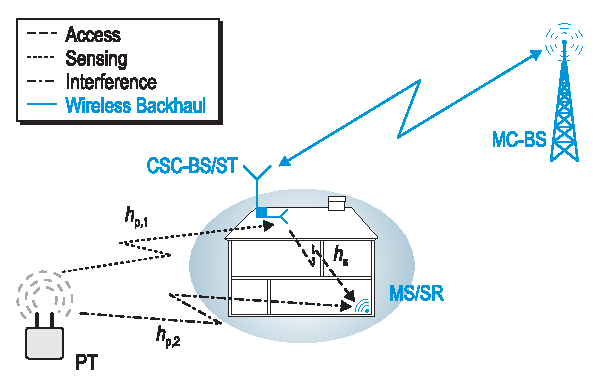
\includegraphics[width = \figscale]{figures/CR_Scenario_Interweave}
\caption{A cognitive small cell scenario demonstrating: (i) the interweave paradigm, (ii) the associated network elements, which constitute cognitive small cell-base station/secondary transmitter (CSC-BS/ST), mobile station/secondary receiver (MS/SR), macro cell-base station (MC-BS) and primary transmitter (PT), (iii) the interacting channels: sensing ($\hpo$), access ($\hs$) and interference ($\hpt$).} 
\label{fig:scenario}
%\vspace{-0.3cm}
\end{figure}
The cognitive small cell (CSC), a CR application, characterizes a small cell deployment that fulfills the spectral requirements for mobile stations (MSs) operating indoor, \tc{refer to} \figurename~\ref{fig:scenario}. For the disposition of the CSC in the network, the following key elements are essential: a CSC-base station (CSC-BS), a macro cell-base station (MC-BS) and MS, refer to \figurename~\ref{fig:scenario}. MSs are the indoor devices served by the CSC-BS over an access channel ($\hs$). Furthermore, the MC-BS is connected to several CSC-BSs over a wireless backhaul\footnote{A wireless backhaul is a point-to-point wireless link between the CSC-BS and MC-BS that relays the traffic generated from the CSC to the core network.}. Moreover, the transmissions from the PT can be listened by the CSC-BS and the MS over sensing ($\hpo$) and interference channel ($\hpt$), respectively. %Although the MC-BS and the MS already exist in the conventional cellular architecture, to incorporate the opportunistic access inside the CSC, it is necessary to consider a functionality upgrade. 
Considering the fact that the IS is employed at the CSC-BS, the CSC-BS and the MS represent a ST and a SR, respectively. A hardware prototype of the CSC-BS operating as IS was presented in \cite{Kaushik13}. For simplification, a PU constraint based on false alarm probability was considered in \cite{Kaushik13}. With the purpose of improving system's reliability, we extend the analysis to employ a PU constraint on the detection probability. 

\tc{Complementing the analysis depicted in \cite{Liang08},} a slotted medium access for the IS is considered, where the time axis is segmented into frames of length $T$, according to which, the ST employs periodic sensing. Hence, each frame consists of a sensing slot $\tsen$ and the remaining duration $T - \tsen$ is utilized for data transmission. For small $T$ relative to the PUs' expected ON/OFF period, the requirement of the ST to be in alignment to PUs' medium access can be relaxed \cite{Wang09, Tang11, Zhao12}.  
 
\subsection{Signal model}
%According to interweave system, ST considers a hypothesis testing to determine the presence ($\mathcal{H}_1$) or absence $(\mathcal{H}_0)$ of a signal transmitted by the PR. 
Subject to the underlying hypothesis that illustrates the presence $(\mathcal{H}_1)$ or absence ($\mathcal{H}_0$) of a PU signal, the discrete and real signal received at the ST is given by  
\begin{equation}
\yrcvd[n] = 
\begin{cases}
\hpo \cdot \xp[n] + w[n] & : \mathcal{H}_1 \\
w[n] & :\mathcal{H}_0
\end{cases},
\label{eq:sys_mod_p1s}
\end{equation}
where $\xp[n]$ corresponds to a discrete and real sample transmitted by the PT, $|\hpo|^2$ represents the power gain of the sensing channel for a given frame and $w[n]$ is additive white Gaussian noise at the ST. \tc{According to \cite{Liang08}, the signal $\xp[n]$ transmitted by the PUs} can be modelled as: (i) a phase shift keying modulated signal, or (ii) a Gaussian signal. The signals that are prone to high inter-symbol interference or entail precoding can be modelled as Gaussian signals. In this chapter, the analysis is focussed on the latter case. As a result, the mean and the variance for the signal and the noise are determined as $\e{}{\xp[n]} = 0$, $\e{}{w[n]} = 0$, $\e{}{|\xp[n]|^2} = \spo$ and $\e{}{|w[n]|^2} = \npo$. The channel $\hpo$ is considered to be independent of $\xp[n]$ and $w[n]$, thus, $\yrcvd$ is also an independent and identically distributed (i.i.d.) random process. %The true received power is defined as
%\begin{align}
%\bprcvd = \e{}{|\yrcvd|^2}.
%\label{eq:tprcvd}
%\end{align}
%Based on (\ref{eq:tprcvd}), the received SNR at the ST is $\snrrcvd = \frac{\bprcvd}{\npo} - 1$.

Similar to (\ref{eq:sys_mod_p1s}), during data transmission, the discrete and real received signal at the SR conditioned on the detection probability ($\pd$) and false alarm probability ($\pfa$) is given by
\begin{equation}
\ys[n] = 
\begin{cases}
\hs \cdot \xs[n] + \hpt \cdot \xp[n] + w[n] & : 1 - \pd \\
\hs \cdot \xs[n] + w[n] & : 1 - \pfa
\end{cases},
\label{eq:sys_mod_ss}
\end{equation}
%and on the other side, the interference signal at the SR, transmitted by the PR follows 
%\begin{equation}
%\yp[n] = \sqrt{\gpt \cdot \apt}/ \cdot \xp[n] + w[n],
%\label{eq:sys_mod_p2s}
%\end{equation}
where $\xs[n]$ corresponds to discrete and real sample transmitted by the ST. Further, $|\hs|^2$ and $|\hpt|^2$ represent the power gains for the access and the interference channels, \tc{refer to} \figurename~\ref{fig:scenario}. 
%The %received powers at the SR from ST and PR are evaluated as $\ps = \s{\test \fsam}{|\ys[n]^2|}$ and $\pp = \s{\test \fsam}{|\yp[n]^2|}$ %Likewise (\ref{eq:sys_mod_p1s}), $\nap[n]$ and $\nas[n]$ represents circularly symmetric AWGN at PR and ST with zero mean and variance $\e{}{|\nap[n]|^2} = \npp$ and $\e{}{|\nas[n]|^2} = \nps$ correspondingly. Consider that $\ps$, $\ps$ and $\pp$ correspond to power for a given frame. 
%\subsubsection{Channel}
%, where $\bpp = \e{}{\pp}$ and $\bps = \e{}{\ps}$ correspond to their true value. Similar to ST-PR, the 
%received SNRs over the links ST-SR and PT-ST are $\snrs = \frac{\e{}{|\sqrt{\hs} \cdot \xs[n]|^2}}{ \npo}$ and $\snrp = \frac{\e{}{|\sqrt{\hpt} \cdot \xp[n]|^2}}{\npo}$.


\section{\tc{Problem Description and Proposed Approach}} \label{sec:pr_mod}
\subsection{\tc{Problem Description}}\label{ssec:pd}
%\subsection{Sensing}
\tc{In accordance with the conventional frame structure}, the ST performs sensing for a duration of $\tsen$. The test statistics $\ts$ at the ST is evaluated as   
\begin{align}
\ts = \s{\tsen \fsam}{ |\yrcvd[n]|^2} \mathop{\gtrless}_{\mathcal{H}_0}^{\mathcal{H}_1} \mu, 
\label{eq:test_st}
\end{align}
where $\mu$ is the decision threshold and $\textbf{y}$ is a vector with $\tsen \fsam$ samples. $\ts$ represents a random variable, whereby the characterization of the distribution function depends on the underlying hypothesis. Corresponding to $\mathcal{H}_0$ and $\mathcal{H}_1$, $\ts$ follows a central chi-squared ($\cchi2$) distribution \cite{Kay}. 
%\begin{equation}
%\ts = 
%\begin{cases}
%\sim \ncchi2  : \mathcal{H}_1 \\
%\sim \cchi2  : \mathcal{H}_0 \\
%\end{cases},
%\label{eq:sys_mod_ss}
%\end{equation}
%Considering large number of samples $\fsam \tsen$ are used to evaluate $\ts$. It is possible to apply Central Limit Theorem to approximate the distribution functions of the mentioned hypotheses as Gaussian distribution. 
As a result, the detection probability $(\pd)$ and the false alarm probability $(\pfa)$ corresponding to (\ref{eq:test_st}) are determined as \cite{Tan08}
\begin{align}
%\pd(\mu, \tsen, \prcvd) &= \mathcal{Q}\left( \frac{\mu - \prcvd}{ \sqrt{\frac{2}{\tsen \fsam}} \prcvd} \right),  \label{eq:pd} 
\pd(\mu, \tsen, \prcvd) &= \Gamma\left( \frac{\tsen \fsam}{2}, \frac{\tsen \fsam \mu}{2 \prcvd} \right),  \label{eq:pd} 
\end{align}
\begin{align}
\pfa(\mu, \tsen) &= \Gamma\left( \frac{\tsen \fsam}{2}, \frac{\tsen \fsam \mu}{2 \npo} \right),  \label{eq:pfa} 
%\pfa(\mu, \tsen) &= \mathcal{Q}\left( \frac{\mu - \npo}{ \sqrt{\frac{2}{\tsen \fsam}} \npo} \right), \label{eq:pfa}
\end{align}
where $\prcvd$ is the power received over the sensing channel and $\Gamma(\cdot, \cdot)$ represents a regularized incomplete upper Gamma function \cite{grad}.% and $\bprcvd$ signifies the true received power defined as
%\begin{align}
%\bprcvd = \e{}{|\yrcvd|^2}.
%\label{eq:tprcvd}
%\end{align}
 %Due to the presence of the estimation received power $\prcvd$ in (\ref{eq:pd}), $\pd$ corresponds to a random variable.

%The detection probability of the primary signal and the throughput achieved at the SR depict the performance of the IS. 

%\subsection{Sensing-Throughput tradeoff}
Following the characterization of $\pfa$ and $\pd$, Liang \textit{et al.} \cite{Liang08} established a tradeoff between the sensing time and secondary throughput $(\rs)$ subject to a target detection probability $(\pdd)$. This tradeoff is represented as  
\begin{align}
\trs(\ttsen) &= \maxi_{\tsen} \rs(\tsen) = \frac{T- \tsen}{T} \bigg[ \cz (1 - \pfa) \phz + \nonumber \\ \quad & \co (1 - \pd) \pho  \bigg], \label{eq:thr_id} \\
\text{s.t.} & \text{ } \pd \ge \pdd, \label{eq:thr_id_con} \\ 
\text{where } & \cz = \log_2 \left(1 + |\hs|^2 \frac{\ptranst}{\npo}\right) = \log_2 \left( 1 + \snrso \right) \label{eq:Cap0}\\ 
{\text{ and }} & \co = \log_2 \left(1 + \frac{|\hs|^2 \ptranst }{|\hpt|^2 \ptranpt  + \npo} \right) \nonumber \\ \quad & = \log_2 \left(1 + \frac{|\hs|^2 \ptranst }{\prcvdsr} \right) = \log_2 \left(1 + \frac{\snrso}{\snrpt + 1}  \right), \label{eq:Cap1} 
\end{align}
where $\phz$ and $\pho$ are the occurrence probabilities for the respective hypothesis, whereas $\snrrcvd$ and $\snrso$ represent the signal to noise ratio for the links PT-ST and ST-SR, respectively, and $\snrpt$ corresponds to interference (from the PT) to noise ratio for the link PT-SR. Moreover, $\ptranpt$ and $\ptranst$ represent the transmit power at the PT and the ST, whereas $\prcvdsr$ corresponds to the received power (which includes the interference power from the PT and the noise power) at the SR. In addition, $\cz$ and $\co$ represent the data rate without and with the interference from the PT. In other words, using (\ref{eq:thr_id}), the ST determines a suitable sensing time $\tsen = \ttsen$, such that the secondary throughput is maximized subject to a target detection probability, \tc{refer to} (\ref{eq:thr_id_con}). From the deployment perspective, the tradeoff depicted above has the following fundamental issues:
\begin{itemize}
\item Without the knowledge of the received power $\prcvd$ over the sensing channel, it is not feasible to characterize $\pd$, refer to (\ref{eq:pd}). This leaves the characterization of the throughput (\ref{eq:thr_id}) impossible and the constraint defined in (\ref{eq:thr_id_con}) inappropriate. 
\item Moreover, the knowledge of the interference and the access channels is required at the ST, \tc{refer to} (\ref{eq:Cap0}) and (\ref{eq:Cap1}) for characterizing the throughput in terms of $\cz$ and $\co$ at the SR. 
\end{itemize}
%Hence, At An optimum performance is achieved when the ST operates at the desired level, i.e., $\pd = \pdd$. %Hence, based on the expression in (\ref{eq:pd}) and constraint in (\ref{eq:thr_id}), the threshold is evaluated as
%\begin{align}
%\mu(\pdd, \tsen, \bprcvd) = \left( \mathcal{Q}^{-1} (\pdd) \sqrt{\frac{2}{\tsen \fsam}} + 1 \right) \bprcvd. \label{eq:lambda} 
%\end{align}
Taking these issues into account, it is not feasible to employ the performance analysis depicted by this model \tc{(referred as ideal model, hereafter)} for hardware implementation. In the subsequent section, an analytical framework \tc{(also referred as estimation model)} that addresses the aforementioned issues, thereby including the estimation of the sensing channel at the ST, and the interference and the access channels at the SR is proposed. Based on the proposed approach, the performance of the IS in terms of the sensing-throughput tradeoff is investigated. 

\subsection{\tc{Proposed Approach}} \label{ssec:pa}

\tc{In order to overcome the difficulties discussed in Section \ref{ssec:pd}, the following strategy is proposed.
\begin{enumerate}
\item As a first step, we consider the estimation of the involved channels. In order to characterize the detection probability, a received power based estimation at the ST for the sensing channel is employed. This is done to ensure that the detection probability remains above a desired level. Further, a pilot based estimation and a received power based estimation for the access channel and the interference channel, respectively, are employed at the SR, to characterize the secondary throughput. 
\item Next, the variations due to channel estimation in the estimated parameters, namely, received power (for the sensing and the interference channels) and the power gain (for the access channel) are characterized in terms of their cumulative distribution functions. 
\item In order to investigate the performance of the IS subject to the channel estimation, these variations in the performance parameters, which include detection probability and secondary throughput, are characterized in terms of their cumulative distribution functions. 
\item Finally, the derived cumulative distribution functions are utlilized to obtain the expressions of sensing-throughput tradeoff. Hence, based on these expressions, the impact of imperfect channel knowledge on performance of the ISs is quatified, and subsequently the achievable secondary throughput at a suitable sensing time is deteremined. 
\end{enumerate}
}

It is well-known that systems with transmitter information (which includes the filter parameters, pilot symbols, modulation type and time-frequency synchronization) at the receiver acquire the channel knowledge by listening to the pilot data sent by the ST \cite{Gans71, Gifford05, Gifford08, Anna05}. Other systems, where the receiver possesses either no access to this information or limited by hardware complexity, procure channel knowledge indirectly by estimating a different parameter that entails the channel knowledge, for instance, received signal power \cite{Kaushik15_CC} or received signal to noise ratio \cite{Chav11, Sharma13}. Recently, estimation techniques such as pilot based estimation \cite{Suraweera10, Kim12} and received power based estimation \cite{Kaushik15} have been applied to obtain channel knowledge for CR systems. However, the performance analysis has been limited to underlay systems, where the emphasis has been given on modelling the interference at the PR. 

Since the pilot based estimation requires the knowledge of the PU signal at the secondary system, the versatility (in terms of PU signals) of the secondary system is compromised. On the other side, for the estimation of the received signal to noise ratio, Eigenvalue (which involves matrix operations) based approach \cite{Sharma13} or iterative approaches such as expectation-maximization have been proposed \cite{Chav11}. Due to the complicated mathematical operations or the complexity of the iterative algorithms, such approaches tend to increase the hardware complexity of the ISs. In order to resolve these issues, a received power based estimation for the sensing and the interference channels, and a pilot based estimation for the access channel is employed. Similar to the energy based detection, since the received power based estimation involves simple operations on the obtained samples such as magnitude squared followed by summation, the proposed estimation provides a reasonable tradoff between complexity and versatility. %Unlike the sensing channel, the access and interference channels have to be estimated at the SR and made available at the ST over a low-rate feedback channel. 
%As a result, by proposing the received power estimation and the pilot based estimation, we the versatility and the low complexity requirements of the CR system, which are absolutely essential from the deployment perspective. 

However, with the inclusion of this channel estimation, the system anticipates: (i) a performance loss in terms of temporal resources used and (ii) variations in the aforementioned performance parameters. A preliminary analysis of this performance loss was carried out in \cite{Kaushik15_CC}, where it was revealed that in low signal to noise ratio regime, imperfect knowledge of received power corresponds to a large variation in the detection probability, hence, causes a severe degradation in the performance of the IS. However, this performance degradation was determined by means of lower and upper bounds. In this chapter, a more exact analysis is considered, whereby the variations in detection probability are captured by characterizing its cumulative distribution function, and subsequently apply new probabilistic constraints on the detection probability, which allow ISs to operate at low signal to noise ratio regime. %These constraints are categorized as average and outage constraints corresponds to an conservative or aggressive approach followed by the SU towards the primary system.   

%Besides that, we include channel estimation at the SR to acquire the knowledge of the access and interference channels. 


%The inclusion of estimation of the interacting channels causes variations in the parameters $\pd$, $\cz$ and $\co$. Unless characterized, these variations may seriously degrade the performance of the hardware deployed. In this view, we include the estimation of the interacting channels in the system model, thereby characterizing the variations in $\pd$, $\cz$ and $\co$ by means of their their distribution functions $\fpd$, $\fcz$ and $\fco$. By utilizing these expressions, we finally obtain a characterization of sensing-throughput tradeoff. %that depicts an deployment scenario. 
In order to include channel estimation, a frame structure that constitutes estimation $\test$, sensing $\tsen$ and data transmission $T - \tsen$ is proposed, where $\test$ and $\tsen$ correspond to time intervals and \tc{$0 < \test \le \tsen < T$, refer to} \figurename~{\ref{fig:fs}}. Since the estimated values of the interacting channels are required for determining the suitable sensing time (the duration of the sensing phase), the sequence depicted in \figurename~{\ref{fig:fs}}, whereby estimation followed by sensing is reasonable for the hardware deployment. 
\tc{Particularly for the sensing channel, it is worthy to note that the samples used for estimation can be combined with the samples acquired for sensing\footnote{\tc{Therefore, the sensing phase incorporates the estimation phase, see \figurename~\ref{fig:fs}}.} such that the time resources within the frame duration can be utilized efficiently, as shown in the frame structure in \figurename~\ref{fig:fs}.} 
To acuqire the estimates for the interference and the access channels at the ST, a low-rate feedback channel from the SR to the ST is required for the proposed approach. 
In the following paragraphs, the estimation of the involved channels is considered. %As $\tsen^{*}$ is dependent on $\prcvd$ or the state of $\hpo$ in particular, under this situation, $\tsen^{*}$ is lower bounded by $\test$, consequently translating $\fpd$ from a continuous function to a piecewise continuous function, thereby complicating the analytical tractability of $\fpd$. Hence, to simplify the analysis, in this work, we consider estimation and sensing as disjoint events in time. In this regard, the derived expressions based on our proposed model represents a lower performance bound. Next, in the following subsections, we present the estimation of the interacting channels. 
\subsubsection{Estimation of sensing channel ($\hpo$)}
\begin{figure}[!ht]
\centering
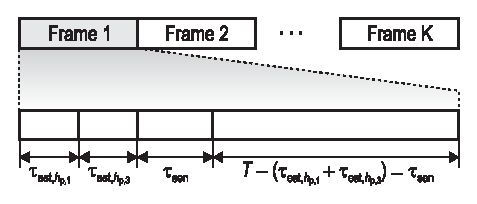
\includegraphics[width = \figscale]{figures/Frame_Structure_grau}
\caption{\tc{An illustration of the proposed frame structure for an interweave system depicting the estimation phase and the sensing phase for the sensing channel.}}
\label{fig:fs}
%\vspace{-0.5cm}
\end{figure}
%To incorporate the effect of fading in the model, we assume that the channel remains constant for $T$. 
Following the previous discussions, the ST acquires the knowledge of $\hpo$ by estimating its received power. The estimated received power is required for the characterization of $\pd$, thereby evaluating the detector performance. %, an vital performance parameter for the cognitive radio system. %Implicit to estimation, the variation in the received power are translated to the $\pd$. Hence, the characterization of the $\pd$ in terms of distribution function is essential. 
%Characterized by the fading process, each frame witnesses a different received power. In order to sustain a desired detection probability, it is important to acquire the knowledge of $\prcvd$. As a result, received power estimation $\test$ precedes sensing $\tsen$ for each frame. The remaining time $T - (\test + \tsen)$ is utilized for data transmission. 

Under $\mathcal H_1$, the received power based estimated during the estimation phase at the ST is given as \cite{Urkowitz} 
\begin{align}
\eprcvd = \s{\test \fsam}{ |\yrcvd[n]|^2}.
\label{eq:eprcvd} 
\end{align}
$\eprcvd$ determined in (\ref{eq:eprcvd}) using $\test \fsam$ samples follows a central chi-squared distribution $\cchi2$ \cite{Kay}. %Applying the central limit theorem, this distribution can be approximated as the Gaussian distribution 
The cumulative distribution function (CDF) of $\eprcvd$ is given by  
\begin{align}
%\eprcvd \sim \mathcal{N}\left( \prcvd, \frac{2}{\test \fsam} \prcvd^2 \right).
%\eprcvd \sim  \cchi\left( \prcvd, \frac{2}{\test \fsam} \prcvd^2 \right).
\feprcvd(x) = 1 - \Gamma\left(\frac{\test \fsam}{2}, \frac{ \test \fsam x}{2 \prcvd}  \right). 
\label{eq:dprcvd}
\end{align}

%Besides estimation of the received power at the ST, the channel estimation of $\hpt$ and $\hs$ is dealt in the following sub-sections. 

\subsubsection{Estimation of access channel ($\hs$)}
%This information is essential for characterize the throughput $\cz$ and $\co$. 
%However, this information is not directly available at the SR.
%To accomplish this, we employ a pilot based estimation for $\hs$ and received power based estimation $\hpt$. 
%Channel estimation is a fundamental aspect to most wireless communication systems. 
The signal received from the ST undergoes matched filtering and demodulation at the SR, hence, it is reasonable to employ pilot based estimation for $\hs$. Unlike received power based estimation, pilot based estimation renders a direct estimation of the channel. 
Now, to accomplish pilot based estimation, the SR aligns itself to pilot symbols transmitted by the ST. Under $\mathcal H_0$, the discrete and real pilot symbols at the output of the demodulator is given by \cite{Gifford08} 
\begin{align}
p[n] = \sqrt{E\sub{s}} \hs + w[n], 
\label{eq:pilot_sig}
\end{align}
where $E\sub{s}$ denotes the pilot energy. Without loss of generality, the pilot symbols are considered to be +1. The maximum likelihood estimate, representing a sample average of $\Ks$ pilot symbols, is given by \cite{Gifford05}
\begin{align}
\hs = \ehs + \smash[b]{\underbrace{\frac{\sum^{\Ks}_{n} p[n]}{2 \Ks}}_{\epsilon}},
\label{eq:pilot_MLE}
\end{align}\\[-0.00em]
where $\epsilon$ denotes the estimation error. 
%(\ref{eq:pilot_MLE}) illustrates a correlation between the $\hs$ and $\ehs$. 
The estimate $\ehs$ is unbiased, efficient and achieves a Cram\'er-Rao bound with equality, with variance $\e{}{|\hs -\ehs|^2} = \npo/(2 \Ks)$ \cite{Gifford08}. Consequently, $\ehs$ conditioned on $\hs$ follows a Gaussian distribution.
\begin{align}
\ehs|\hs \sim \mathcal{N}\left( \hs,\evar \right).
\label{eq:ehs} 
\end{align}
As a result, the power gain $|\ehs|^2$ follows a non-central chi-squared ($\ncchi2$) distribution with 1 degree of freedom and non-centrality parameter $\ls = \frac{2 \Ks |\hs|^2}{\npo}$.  

\subsubsection{Estimation of interference channel ($\hpt$)}
Analog to the sensing channel, the SR performs received power based estimation by listening to the transmission from the PT. The knowledge of $\hpt$ is required to characterize interference from the PT. Under $\mathcal H_1$, the discrete signal model at the SR is given as 
\begin{align}
\ys[n] = \hpt \cdot \xp[n] + w[n].
\label{eq:sys_mod_p2s}
\end{align}
The received power at the SR from the PT given by  
\begin{align} 
\eprcvdsr &= \frac{1}{\Kp} \sum\limits_{n = 1}^{\Kp} |\ys[n]|^2,
\label{eq:ehp2}
\end{align}
follows a $\cchi2$ distribution, where $\Kp$ corresponds to the number of samples used for the estimation.

\subsection{\tc{Validation}}
\tc{
It is now clear that the estimates $\eprcvd$, $|\ehs|^2$ and $\eprcvdsr$ exhibit the knowledge corresponding to the involved channels, however, it is essential to validate them, mainly $\eprcvd$ and $\eprcvdsr$. In this context, it is necessary to ensure the presence of the PU signal ($\mathcal H_1$) for that particular frame. In this direction, Chavali \textit{et al.} \cite{Chav11} recently proposed a detection followed by the estimation of the signal to noise ratio, while \cite{Cao14} implemented a blind technique for estimating the signal power of non-coherent PU signals. In this thesis, a different methodology is proposed, according to which, a coarse detection\footnote{\tc{For the coarse detection, an energy detection is employed whose threshold can be determined by means of a constant false alarm rate.}} on the estimates $\eprcvd$, $\eprcvdsr$ at the end of the estimation phase $\test$ is applied. Through an appropriate selection of the time interval $\test$ (for instance, $\test \in [1, 10]\SI{}{ms}$) during the system design, the reliability of the coarse detection can be ensured. With the existence of a separate control channel such as cognitive pilot channel, the reliability of the coarse detection can be further enhanced by exchanging the detection results between the ST and the SR.} 

\tc{
Since the estimation and the coarse detection processes in the proposed method are equivalent in terms of their mathematical operations (which include magnitude squared and summation), the validity of the channel estimates with certain reliability and without comprising the complexity of the estimators employed by the secondary system is considered. Moreover, by performing a joint estimation and (coarse) detection, an efficient way of utilizing the time resources within the frame duration is proposed. The ST considers these estimates to determine a suitable sensing time based on the sensing-throughput tradeoff such that the desired detector's performance is ensured. At the end of the detection phase, a fine detection\footnote{\tc{In accordance with the proposed frame structure in Fig. 2, fine detection represents the main detection which also includes the samples acquired during the estimation phase.}} of the PU signals is carried out, thereby improving the performance of the detector.} 
  
\subsection{Assumptions and Approximations}
%We consider the estimation of $\bprcvd$ at the ST. To simplify the analysis for the proposed model, it is assumed that the ST acquires the perfect knowledge about $\snrp$ and $ \snrs$ from the SR over a feedback channel. 
To simplify the analysis and sustain analytical tractability for the proposed approach, several assumptions considered in the chapter are summarized as follows:
\begin{itemize}
\item All transmitted signals are subjected to distance dependent path loss and small scale fading gain. %The small scale fading gains $\gpo, \gpt, \gs$ are modelled as frequency-flat fading. %Hence, the $\gpo, \gpt, \gs$ follow a unit-mean exponential distribution \cite{Tse05}.
With no loss of generality, it is considered that the channel gains include distance dependent path loss and small scale gain. Moreover, the coherence time for the channel gain is considered to be greater than the frame duration\footnote{In the scenarios where the coherence time exceeds the frame duration, in such cases, the proposed characterization depicts a lower performance bound.}. 
%Finally, we target short-term policy, we optimize the performance for each frame.
%\item We consider that all transmitted signals are subjected to distance dependent path loss and the small scale fading gains. The coherence time for the channel gain is greater than the frame duration. %The small scale fading gains $\gpo, \gpt, \gs$ are modelled as frequency-flat fading. Hence, the $\gpo, \gpt, \gs$ follow a unit-mean exponential distribution \cite{Tse05}.
%With no loss of generality, we consider that the channel gains include distance dependent path loss and small scale gain. %Finally, we target short-term policy, we optimize the performance for each frame.
%\item To ensure mathematical tractability of the proposed model, we consider disjoint sets of samples for estimation and sensing for a certain frame. However, in practice, it is possible to utilize the samples used in the estimation phase for sensing purpose as well, which leads to an improvement in the detector's performance in terms of the number of samples utilized for sensing. 
%\item As the estimation and sensing involves the summation of a large number of samples, where each sample is independent and follows $\ncchi2$ distribution, we apply Central limit theorem to approximate the $\ncchi2$ distribution as Gaussian ($\mathcal N$) distribution \cite{Tan08, Liang08}. The parameters of $\mathcal N$ distribution is computed by comparing its first two central moments with the $\ncchi2$.  
\item Perfect knowledge of the noise power is assumend in the system, however, the uncertainty in noise power can be captured as a bounded interval \cite{Tan08}. Inserting this interval in the derived expressions, \tc{refer to} Section \ref{sec:ana}, the performance of the IS can be expressed in terms of the upper and the lower bounds. 
\item For all degrees of freedom, $\ncchi2$ distribution can be approximated by Gamma distribution \cite{abramo}. The parameters of the Gamma distribution are obtained by matching the first two central moments to those of $\ncchi2$. 
%\item Analog to \cite{Liang08, Juarez11, Sharkasi12, Pradhan15}, the proposed model stipulates the knowledge of the underlying hypothesis at the ST and the SR. With the knowledge of occurrence probabilities $\phz$ and $\pho$ and subsequently applying PU traffic models proposed in \cite{Wang09, Tang11, Zhao12}, it is possible to acquire this knowledge with high probability. 
%Moreover, it is reasonable that the ST and the SR perform estimation independently. 
%\item Considering a realistic situation, it is possible that SR might not accomplish estimation in each frame, under such circumstances, the ST utilizes the previous estimation value for the sensing-throughput analysis. %Hence, it is sufficient to incorporate $\test \fsam$ in the expression of the throughput.  
\end{itemize}


\section{Theoretical Analysis} \label{sec:ana}
%%%%%%%%%%%%%%%%%%%%%%%%%%%%%%%%%%%%%%%%%%%%%%%%%%%%%%%%%%%%%%%%%%%%%%%%%%%%%%%%%%%%%%%%%
%\subsection*{Characterizing the performance parameters}
%%%%%%%%%%%%%%%%%%%%%%%%%%%%%%%%%%%%%%%%%%%%%%%%%%%%%%%%%%%%%%%%%%%%%%%%%%%%%%%%%%%%%%%%%%
%The estimation of received power at the ST and interacting channels translate to the distortion in the performance parameters $\pd$ and $\trs$. 
%While substituting estimated received power $\prcvd$ in (\ref{eq:pd}), a certain distortion is induced in the $\pd$. In order capture this distortion, it is essential to characterize its distribution function $\fpd$. 

\subsection{Deterministic Channel} \label{ssec:det_th}
At first, the performance of the proposed framework in context to the deterministic channel is evaluated.
It is evident that the variation due to the imperfect channel knowledge translates to the variations of the performance parameters $\epd, \ecz$ and $\eco$, which are fundamental to sensing-throughput tradeoff. Below, these variations are captured by characterizing their cumulative distribution functions $\fpd$, $\fcz$ and $\fco$, respectively.  
\begin{lemma} \label{lm:lem1}
\normalfont
The cumulative distribution function of $\epd$ is characterized as 
\begin{align}
\fpd(x) = 1 - \Gamma \left(\frac{\test \fsam}{2}, \frac{\test \tsen \fsam^2 \mu}{4 \prcvd \Gamma^{-1}(x, \frac{\tsen \fsam}{2}) } \right), 
%\fpd(x) = 1 - \mathcal{Q} \left( {\frac{\mu}{ \left( \sqrt{\frac{2}{\tsen \fsam}} \mathcal{Q}^{-1}(x) + 1 \right) }}\Bigg/{ \sqrt{\frac{2}{\test \fsam}} \prcvd }  \right).
%\dpd = \mu \frac{\exp \left( \frac{\left(\mathcal{Q}^{-1}(x)\right)^2}{2}  - \left( \frac{\frac{\lambda}{1 + \sqrt{\frac{2}{\tsen \fsam}} \mathcal{Q}^{-1}(x)} - \bprcvd}{ \bprcvd \sqrt{\frac{4}{\test \fsam}}}    \right)^2 \right)}{ \bprcvd \sqrt{\frac{2}{\tsen \fsam}} \left( 1 + \sqrt{\frac{2}{\test \fsam}} \mathcal{Q}^{-1}(x) \right)^2 }
\label{eq:fpd}
\end{align}
where $\Gamma^{-1}(\cdot, \cdot)$ is inverse function of regularized upper incomplete Gamma function \cite{grad}.  
\end{lemma} 
\begin{IEEEproof}
The cumulative distribution function of $\epd$ is defined as 
\begin{align}
\fpd(x) = \p(\epd \le x).
\end{align}
Using (\ref{eq:pd})
\begin{align}
\quad =  \p \left( \Gamma \left( \frac{\tsen \fsam}{2}, \frac{\tsen \fsam \mu}{2 \eprcvd} \right) \le x \right), 
\end{align}
\begin{align}
\quad =  1- \p \left( \eprcvd \ge \frac{\mu \tsen \fsam}{2 {\Gamma}^{-1}\left( x, \frac{\tsen \fsam}{2} \right) } \right). \label{eq:lem1} 
%\quad &=  \p \left( \mathcal{Q} \left( \frac{\mu - \eprcvd}{\sqrt{\frac{2}{\tsen \fsam} }} \right) \le x \right) \\ 
%\quad &=  1- \p \left( \eprcvd \le \frac{\mu}{\mathcal{Q}^{-1}(x) \sqrt{\frac{2}{\tsen \fsam}}} \right) 
\end{align}
Replacing the cumulative distribution function of $\eprcvd$ in (\ref{eq:lem1}), an expression of $\fpd$ is obtained.
\end{IEEEproof}
%From (\ref{eq:fpd}), it is clearly observed that $\fpd$ depends on $\prcvd$, $\tsen$ and $\test$. %This insight will be discussed in later analysis.
%Now, ST precludes the primary system by sustaining the $\pd$ above a certain desired level $\pdd$
%\begin{align}
%\pd(\mu, \tsen, \bprcvd) \ge \pdd. \label{eq:pdc}  
%\end{align}
%%%%%%%%%%%%%%%%%%%%%%%%%%%%%%%%%%%%%%%%%%%%%%%%%%%%%%%%%%%%%%%%%%%%%%%%%%%%%%%%%%%%%%%%%
%\subsection*{Distortion in throughput}
%%%%%%%%%%%%%%%%%%%%%%%%%%%%%%%%%%%%%%%%%%%%%%%%%%%%%%%%%%%%%%%%%%%%%%%%%%%%%%%%%%%%%%%%%
%Due to the estimation of the interacting channels a certain amount of distortion is introduced in the throughput. 

\captionsetup[subfigure]{position=top}
\begin{figure}[!ht]
\centering
\subfloat[]{
% This file is generated by the MATLAB m-file laprint.m. It can be included
% into LaTeX documents using the packages graphicx, color and psfrag.
% It is accompanied by a postscript file. A sample LaTeX file is:
%    \documentclass{article}\usepackage{graphicx,color,psfrag}
%    \begin{document}% This file is generated by the MATLAB m-file laprint.m. It can be included
% into LaTeX documents using the packages graphicx, color and psfrag.
% It is accompanied by a postscript file. A sample LaTeX file is:
%    \documentclass{article}\usepackage{graphicx,color,psfrag}
%    \begin{document}\input{fig_CDF_pd_diff_test}\end{document}
% See http://www.mathworks.de/matlabcentral/fileexchange/loadFile.do?objectId=4638
% for recent versions of laprint.m.
%
% created by:           LaPrint version 3.16 (13.9.2004)
% created on:           30-Nov-2015 14:08:24
% eps bounding box:     16 cm x 12 cm
% comment:              
%
%\begin{psfrags}%
%\psfragscanon%
%
% text strings:
\psfrag{s05}[t][t]{\fontsize{8}{12}\fontseries{m}\mathversion{normal}\fontshape{n}\selectfont \color[rgb]{0,0,0}\setlength{\tabcolsep}{0pt}\begin{tabular}{c}$\pd$\end{tabular}}%
\psfrag{s06}[b][b]{\fontsize{8}{12}\fontseries{m}\mathversion{normal}\fontshape{n}\selectfont \color[rgb]{0,0,0}\setlength{\tabcolsep}{0pt}\begin{tabular}{c}CDF\end{tabular}}%
\psfrag{s10}[][]{\fontsize{10}{15}\fontseries{m}\mathversion{normal}\fontshape{n}\selectfont \color[rgb]{0,0,0}\setlength{\tabcolsep}{0pt}\begin{tabular}{c} \end{tabular}}%
\psfrag{s11}[][]{\fontsize{10}{15}\fontseries{m}\mathversion{normal}\fontshape{n}\selectfont \color[rgb]{0,0,0}\setlength{\tabcolsep}{0pt}\begin{tabular}{c} \end{tabular}}%
\psfrag{s12}[l][l]{\fontsize{8}{12}\fontseries{m}\mathversion{normal}\fontshape{n}\selectfont \color[rgb]{0,0,0}Simulated}%
\psfrag{s13}[l][l]{\fontsize{8}{12}\fontseries{m}\mathversion{normal}\fontshape{n}\selectfont \color[rgb]{0,0,0}Theoretical}%
\psfrag{s14}[l][l]{\fontsize{8}{12}\fontseries{m}\mathversion{normal}\fontshape{n}\selectfont \color[rgb]{0,0,0}Simulated}%
%
% axes font properties:
\fontsize{8}{12}\fontseries{m}\mathversion{normal}%
\fontshape{n}\selectfont%
%
% xticklabels:
\psfrag{x01}[t][t]{0}%
\psfrag{x02}[t][t]{0.1}%
\psfrag{x03}[t][t]{0.2}%
\psfrag{x04}[t][t]{0.3}%
\psfrag{x05}[t][t]{0.4}%
\psfrag{x06}[t][t]{0.5}%
\psfrag{x07}[t][t]{0.6}%
\psfrag{x08}[t][t]{0.7}%
\psfrag{x09}[t][t]{0.8}%
\psfrag{x10}[t][t]{0.9}%
\psfrag{x11}[t][t]{1}%
%
% yticklabels:
\psfrag{v01}[r][r]{0}%
\psfrag{v02}[r][r]{0.1}%
\psfrag{v03}[r][r]{0.2}%
\psfrag{v04}[r][r]{0.3}%
\psfrag{v05}[r][r]{0.4}%
\psfrag{v06}[r][r]{0.5}%
\psfrag{v07}[r][r]{0.6}%
\psfrag{v08}[r][r]{0.7}%
\psfrag{v09}[r][r]{0.8}%
\psfrag{v10}[r][r]{0.9}%
\psfrag{v11}[r][r]{1}%
%
% Figure:
%\resizebox{8cm}{!}{\includegraphics{fig_CDF_pd_diff_test.eps}}%
%\end{psfrags}%
%
% End fig_CDF_pd_diff_test.tex
\end{document}
% See http://www.mathworks.de/matlabcentral/fileexchange/loadFile.do?objectId=4638
% for recent versions of laprint.m.
%
% created by:           LaPrint version 3.16 (13.9.2004)
% created on:           30-Nov-2015 14:08:24
% eps bounding box:     16 cm x 12 cm
% comment:              
%
%\begin{psfrags}%
%\psfragscanon%
%
% text strings:
\psfrag{s05}[t][t]{\fontsize{8}{12}\fontseries{m}\mathversion{normal}\fontshape{n}\selectfont \color[rgb]{0,0,0}\setlength{\tabcolsep}{0pt}\begin{tabular}{c}$\pd$\end{tabular}}%
\psfrag{s06}[b][b]{\fontsize{8}{12}\fontseries{m}\mathversion{normal}\fontshape{n}\selectfont \color[rgb]{0,0,0}\setlength{\tabcolsep}{0pt}\begin{tabular}{c}CDF\end{tabular}}%
\psfrag{s10}[][]{\fontsize{10}{15}\fontseries{m}\mathversion{normal}\fontshape{n}\selectfont \color[rgb]{0,0,0}\setlength{\tabcolsep}{0pt}\begin{tabular}{c} \end{tabular}}%
\psfrag{s11}[][]{\fontsize{10}{15}\fontseries{m}\mathversion{normal}\fontshape{n}\selectfont \color[rgb]{0,0,0}\setlength{\tabcolsep}{0pt}\begin{tabular}{c} \end{tabular}}%
\psfrag{s12}[l][l]{\fontsize{8}{12}\fontseries{m}\mathversion{normal}\fontshape{n}\selectfont \color[rgb]{0,0,0}Simulated}%
\psfrag{s13}[l][l]{\fontsize{8}{12}\fontseries{m}\mathversion{normal}\fontshape{n}\selectfont \color[rgb]{0,0,0}Theoretical}%
\psfrag{s14}[l][l]{\fontsize{8}{12}\fontseries{m}\mathversion{normal}\fontshape{n}\selectfont \color[rgb]{0,0,0}Simulated}%
%
% axes font properties:
\fontsize{8}{12}\fontseries{m}\mathversion{normal}%
\fontshape{n}\selectfont%
%
% xticklabels:
\psfrag{x01}[t][t]{0}%
\psfrag{x02}[t][t]{0.1}%
\psfrag{x03}[t][t]{0.2}%
\psfrag{x04}[t][t]{0.3}%
\psfrag{x05}[t][t]{0.4}%
\psfrag{x06}[t][t]{0.5}%
\psfrag{x07}[t][t]{0.6}%
\psfrag{x08}[t][t]{0.7}%
\psfrag{x09}[t][t]{0.8}%
\psfrag{x10}[t][t]{0.9}%
\psfrag{x11}[t][t]{1}%
%
% yticklabels:
\psfrag{v01}[r][r]{0}%
\psfrag{v02}[r][r]{0.1}%
\psfrag{v03}[r][r]{0.2}%
\psfrag{v04}[r][r]{0.3}%
\psfrag{v05}[r][r]{0.4}%
\psfrag{v06}[r][r]{0.5}%
\psfrag{v07}[r][r]{0.6}%
\psfrag{v08}[r][r]{0.7}%
\psfrag{v09}[r][r]{0.8}%
\psfrag{v10}[r][r]{0.9}%
\psfrag{v11}[r][r]{1}%
%
% Figure:
%\resizebox{8cm}{!}{\includegraphics{fig_CDF_pd_diff_test.eps}}%
%\end{psfrags}%
%
% End fig_CDF_pd_diff_test.tex

\begin{tikzpicture}[scale=1]
\node[anchor=south west,inner sep=0] (image) at (0,0)
{
	\includegraphics[width = \figscale]{figures/fig_CDF_pd_diff_test}
};
\begin{scope}[x={(image.south east)},y={(image.north west)}]
\draw[black,->] (0.62,0.3) -- (0.82,0.13);
\node[draw=none, font=\scriptsize] at (0.57,0.35) {$\test \in \{1,5,10\} \SI{}{ms}$};
%\draw[help lines,xstep=.1,ystep=.1] (0,0) grid (1,1);
%\foreach \x in {0,1,...,9} { \node [anchor=north] at (\x/10,0) {0.\x}; }
%\foreach \y in {0,1,...,9} { \node [anchor=east] at (0,\y/10) {0.\y}; }
\end{scope}
\end{tikzpicture} 
\quad \label{fig:CDF_pd_test}
}
\hfil
\subfloat[]{
% This file is generated by the MATLAB m-file laprint.m. It can be included
% into LaTeX documents using the packages graphicx, color and psfrag.
% It is accompanied by a postscript file. A sample LaTeX file is:
%    \documentclass{article}\usepackage{graphicx,color,psfrag}
%    \begin{document}% This file is generated by the MATLAB m-file laprint.m. It can be included
% into LaTeX documents using the packages graphicx, color and psfrag.
% It is accompanied by a postscript file. A sample LaTeX file is:
%    \documentclass{article}\usepackage{graphicx,color,psfrag}
%    \begin{document}\input{fig_CDF_pd_diff_tsen}\end{document}
% See http://www.mathworks.de/matlabcentral/fileexchange/loadFile.do?objectId=4638
% for recent versions of laprint.m.
%
% created by:           LaPrint version 3.16 (13.9.2004)
% created on:           30-Nov-2015 14:08:07
% eps bounding box:     14 cm x 10.5 cm
% comment:              
%
%\begin{psfrags}%
%\psfragscanon%
%
% text strings:
\psfrag{s05}[t][t]{\fontsize{8}{12}\fontseries{m}\mathversion{normal}\fontshape{n}\selectfont \color[rgb]{0,0,0}\setlength{\tabcolsep}{0pt}\begin{tabular}{c}$\pd$\end{tabular}}%
\psfrag{s06}[b][b]{\fontsize{8}{12}\fontseries{m}\mathversion{normal}\fontshape{n}\selectfont \color[rgb]{0,0,0}\setlength{\tabcolsep}{0pt}\begin{tabular}{c}CDF\end{tabular}}%
\psfrag{s10}[][]{\fontsize{10}{15}\fontseries{m}\mathversion{normal}\fontshape{n}\selectfont \color[rgb]{0,0,0}\setlength{\tabcolsep}{0pt}\begin{tabular}{c} \end{tabular}}%
\psfrag{s11}[][]{\fontsize{10}{15}\fontseries{m}\mathversion{normal}\fontshape{n}\selectfont \color[rgb]{0,0,0}\setlength{\tabcolsep}{0pt}\begin{tabular}{c} \end{tabular}}%
\psfrag{s12}[l][l]{\fontsize{8}{12}\fontseries{m}\mathversion{normal}\fontshape{n}\selectfont \color[rgb]{0,0,0}Simulated}%
\psfrag{s13}[l][l]{\fontsize{8}{12}\fontseries{m}\mathversion{normal}\fontshape{n}\selectfont \color[rgb]{0,0,0}Theoretical}%
\psfrag{s14}[l][l]{\fontsize{8}{12}\fontseries{m}\mathversion{normal}\fontshape{n}\selectfont \color[rgb]{0,0,0}Simulated}%
%
% axes font properties:
\fontsize{8}{12}\fontseries{m}\mathversion{normal}%
\fontshape{n}\selectfont%
%
% xticklabels:
\psfrag{x01}[t][t]{0}%
\psfrag{x02}[t][t]{0.2}%
\psfrag{x03}[t][t]{0.4}%
\psfrag{x04}[t][t]{0.6}%
\psfrag{x05}[t][t]{0.8}%
\psfrag{x06}[t][t]{1}%
%
% yticklabels:
\psfrag{v01}[r][r]{0}%
\psfrag{v02}[r][r]{0.1}%
\psfrag{v03}[r][r]{0.2}%
\psfrag{v04}[r][r]{0.3}%
\psfrag{v05}[r][r]{0.4}%
\psfrag{v06}[r][r]{0.5}%
\psfrag{v07}[r][r]{0.6}%
\psfrag{v08}[r][r]{0.7}%
\psfrag{v09}[r][r]{0.8}%
\psfrag{v10}[r][r]{0.9}%
\psfrag{v11}[r][r]{1}%
%
% Figure:
%\resizebox{7cm}{!}{\includegraphics{fig_CDF_pd_diff_tsen.eps}}%
%\end{psfrags}%
%
% End fig_CDF_pd_diff_tsen.tex
\end{document}
% See http://www.mathworks.de/matlabcentral/fileexchange/loadFile.do?objectId=4638
% for recent versions of laprint.m.
%
% created by:           LaPrint version 3.16 (13.9.2004)
% created on:           30-Nov-2015 14:08:07
% eps bounding box:     14 cm x 10.5 cm
% comment:              
%
%\begin{psfrags}%
%\psfragscanon%
%
% text strings:
\psfrag{s05}[t][t]{\fontsize{8}{12}\fontseries{m}\mathversion{normal}\fontshape{n}\selectfont \color[rgb]{0,0,0}\setlength{\tabcolsep}{0pt}\begin{tabular}{c}$\pd$\end{tabular}}%
\psfrag{s06}[b][b]{\fontsize{8}{12}\fontseries{m}\mathversion{normal}\fontshape{n}\selectfont \color[rgb]{0,0,0}\setlength{\tabcolsep}{0pt}\begin{tabular}{c}CDF\end{tabular}}%
\psfrag{s10}[][]{\fontsize{10}{15}\fontseries{m}\mathversion{normal}\fontshape{n}\selectfont \color[rgb]{0,0,0}\setlength{\tabcolsep}{0pt}\begin{tabular}{c} \end{tabular}}%
\psfrag{s11}[][]{\fontsize{10}{15}\fontseries{m}\mathversion{normal}\fontshape{n}\selectfont \color[rgb]{0,0,0}\setlength{\tabcolsep}{0pt}\begin{tabular}{c} \end{tabular}}%
\psfrag{s12}[l][l]{\fontsize{8}{12}\fontseries{m}\mathversion{normal}\fontshape{n}\selectfont \color[rgb]{0,0,0}Simulated}%
\psfrag{s13}[l][l]{\fontsize{8}{12}\fontseries{m}\mathversion{normal}\fontshape{n}\selectfont \color[rgb]{0,0,0}Theoretical}%
\psfrag{s14}[l][l]{\fontsize{8}{12}\fontseries{m}\mathversion{normal}\fontshape{n}\selectfont \color[rgb]{0,0,0}Simulated}%
%
% axes font properties:
\fontsize{8}{12}\fontseries{m}\mathversion{normal}%
\fontshape{n}\selectfont%
%
% xticklabels:
\psfrag{x01}[t][t]{0}%
\psfrag{x02}[t][t]{0.2}%
\psfrag{x03}[t][t]{0.4}%
\psfrag{x04}[t][t]{0.6}%
\psfrag{x05}[t][t]{0.8}%
\psfrag{x06}[t][t]{1}%
%
% yticklabels:
\psfrag{v01}[r][r]{0}%
\psfrag{v02}[r][r]{0.1}%
\psfrag{v03}[r][r]{0.2}%
\psfrag{v04}[r][r]{0.3}%
\psfrag{v05}[r][r]{0.4}%
\psfrag{v06}[r][r]{0.5}%
\psfrag{v07}[r][r]{0.6}%
\psfrag{v08}[r][r]{0.7}%
\psfrag{v09}[r][r]{0.8}%
\psfrag{v10}[r][r]{0.9}%
\psfrag{v11}[r][r]{1}%
%
% Figure:
%\resizebox{7cm}{!}{\includegraphics{fig_CDF_pd_diff_tsen.eps}}%
%\end{psfrags}%
%
% End fig_CDF_pd_diff_tsen.tex

\begin{tikzpicture}[scale=1]
\node[anchor=south west,inner sep=0] (image) at (0,0)
{
	\includegraphics[width = \figscale]{figures/fig_CDF_pd_diff_tsen}
};
\begin{scope}[x={(image.south east)},y={(image.north west)}]
\draw[black,<-] (0.5,0.45) -- (0.68,0.21); 
\node[draw=none, font=\scriptsize] at (0.73,0.16) {$\tsen \in \{1,5,10\} \SI{}{ms}$};
%\draw[help lines,xstep=.1,ystep=.1] (0,0) grid (1,1);
%\foreach \x in {0,1,...,9} { \node [anchor=north] at (\x/10,0) {0.\x}; }
%\foreach \y in {0,1,...,9} { \node [anchor=east] at (0,\y/10) {0.\y}; }
\end{scope}
\end{tikzpicture}
\quad
\label{fig:CDF_pd_tsen}}
\vspace{0.3cm}
\caption{CDF of $\epd$ for different $\test$ and $\tsen$. (a) $\test \in \{1,5,10\} \SI{}{ms}$ and $\tsen = \SI{1}{ms}$, (b) $\test = \SI{1}{ms}$ and $\tsen \in \{1,5,10\} \SI{}{ms}$.}
\label{fig:CDF_pd}
%\vspace{-0.5cm}
\end{figure}


\begin{lemma} \label{lm:lem2}
\normalfont
The cumulative distribution function of $\ecz$ is defined as
\begin{align}
\fcz(x) &= \int\limits_{0}^{x} \dcz(t) dt, \label{eq:dis_C0} 
\end{align}
where
\begin{align}
\dcz(x) &= 2^x \ln 2 \frac{(2^x - 1)^{\as - 1}}{\Gamma(\as) \bs^{\as}} \exp\left(-\frac{2^x - 1}{\bs}\right),  \label{eq:den_C0}
\end{align}
and  
\begin{align}
\quad & \as = \frac{\left(\lambdas + |\hs|^2  \right)^2 }{ \lambdas \left(2 \lambdas + 4 |\hs|^2  \right)}   \text{  and  } \nonumber \\ \quad & \bs = \frac{\lambdas \left(2 \lambdas + 4  |\hs|^2 \right)}{\left( \lambdas + |\hs|^2  \right) } \label{eq:para_s}. 
\end{align}
\end{lemma} 
\begin{IEEEproof}
\tc{See Section \ref{ssec:lem2}}
\end{IEEEproof}

\begin{figure}[!ht]

%% Add psfrag entries
% This file is generated by the MATLAB m-file laprint.m. It can be included
% into LaTeX documents using the packages graphicx, color and psfrag.
% It is accompanied by a postscript file. A sample LaTeX file is:
%    \documentclass{article}\usepackage{graphicx,color,psfrag}
%    \begin{document}% This file is generated by the MATLAB m-file laprint.m. It can be included
% into LaTeX documents using the packages graphicx, color and psfrag.
% It is accompanied by a postscript file. A sample LaTeX file is:
%    \documentclass{article}\usepackage{graphicx,color,psfrag}
%    \begin{document}\input{fig_CDF_C0_diff_SNR_s}\end{document}
% See http://www.mathworks.de/matlabcentral/fileexchange/loadFile.do?objectId=4638
% for recent versions of laprint.m.
%
% created by:           LaPrint version 3.16 (13.9.2004)
% created on:           30-Nov-2015 14:08:58
% eps bounding box:     16 cm x 12 cm
% comment:              
%
%\begin{psfrags}%
%\psfragscanon%
%
% text strings:
\psfrag{s05}[t][t]{\fontsize{8}{12}\fontseries{m}\mathversion{normal}\fontshape{n}\selectfont \color[rgb]{0,0,0}\setlength{\tabcolsep}{0pt}\begin{tabular}{c}$\ecz$ [bits/sec/Hz]\end{tabular}}%
\psfrag{s06}[b][b]{\fontsize{8}{12}\fontseries{m}\mathversion{normal}\fontshape{n}\selectfont \color[rgb]{0,0,0}\setlength{\tabcolsep}{0pt}\begin{tabular}{c}CDF\end{tabular}}%
\psfrag{s10}[][]{\fontsize{10}{15}\fontseries{m}\mathversion{normal}\fontshape{n}\selectfont \color[rgb]{0,0,0}\setlength{\tabcolsep}{0pt}\begin{tabular}{c} \end{tabular}}%
\psfrag{s11}[][]{\fontsize{10}{15}\fontseries{m}\mathversion{normal}\fontshape{n}\selectfont \color[rgb]{0,0,0}\setlength{\tabcolsep}{0pt}\begin{tabular}{c} \end{tabular}}%
\psfrag{s12}[l][l]{\fontsize{8}{12}\fontseries{m}\mathversion{normal}\fontshape{n}\selectfont \color[rgb]{0,0,0}Simulated}%
\psfrag{s13}[l][l]{\fontsize{8}{12}\fontseries{m}\mathversion{normal}\fontshape{n}\selectfont \color[rgb]{0,0,0}(\ref{eq_IS:dis_C0})}%
\psfrag{s14}[l][l]{\fontsize{8}{12}\fontseries{m}\mathversion{normal}\fontshape{n}\selectfont \color[rgb]{0,0,0}Simulated}%
%
% axes font properties:
\fontsize{8}{12}\fontseries{m}\mathversion{normal}%
\fontshape{n}\selectfont%
%
% xticklabels:
\psfrag{x01}[t][t]{0}%
\psfrag{x02}[t][t]{0.5}%
\psfrag{x03}[t][t]{1}%
\psfrag{x04}[t][t]{1.5}%
\psfrag{x05}[t][t]{2}%
\psfrag{x06}[t][t]{2.5}%
\psfrag{x07}[t][t]{3}%
\psfrag{x08}[t][t]{3.5}%
\psfrag{x09}[t][t]{4}%
\psfrag{x10}[t][t]{4.5}%
%
% yticklabels:
\psfrag{v01}[r][r]{0}%
\psfrag{v02}[r][r]{0.1}%
\psfrag{v03}[r][r]{0.2}%
\psfrag{v04}[r][r]{0.3}%
\psfrag{v05}[r][r]{0.4}%
\psfrag{v06}[r][r]{0.5}%
\psfrag{v07}[r][r]{0.6}%
\psfrag{v08}[r][r]{0.7}%
\psfrag{v09}[r][r]{0.8}%
\psfrag{v10}[r][r]{0.9}%
\psfrag{v11}[r][r]{1}%
%
% Figure:
%\resizebox{8cm}{!}{\includegraphics{fig_CDF_C0_diff_SNR_s.eps}}%
%\end{psfrags}%
%
% End fig_CDF_C0_diff_SNR_s.tex
\end{document}
% See http://www.mathworks.de/matlabcentral/fileexchange/loadFile.do?objectId=4638
% for recent versions of laprint.m.
%
% created by:           LaPrint version 3.16 (13.9.2004)
% created on:           30-Nov-2015 14:08:58
% eps bounding box:     16 cm x 12 cm
% comment:              
%
%\begin{psfrags}%
%\psfragscanon%
%
% text strings:
\psfrag{s05}[t][t]{\fontsize{8}{12}\fontseries{m}\mathversion{normal}\fontshape{n}\selectfont \color[rgb]{0,0,0}\setlength{\tabcolsep}{0pt}\begin{tabular}{c}$\ecz$ [bits/sec/Hz]\end{tabular}}%
\psfrag{s06}[b][b]{\fontsize{8}{12}\fontseries{m}\mathversion{normal}\fontshape{n}\selectfont \color[rgb]{0,0,0}\setlength{\tabcolsep}{0pt}\begin{tabular}{c}CDF\end{tabular}}%
\psfrag{s10}[][]{\fontsize{10}{15}\fontseries{m}\mathversion{normal}\fontshape{n}\selectfont \color[rgb]{0,0,0}\setlength{\tabcolsep}{0pt}\begin{tabular}{c} \end{tabular}}%
\psfrag{s11}[][]{\fontsize{10}{15}\fontseries{m}\mathversion{normal}\fontshape{n}\selectfont \color[rgb]{0,0,0}\setlength{\tabcolsep}{0pt}\begin{tabular}{c} \end{tabular}}%
\psfrag{s12}[l][l]{\fontsize{8}{12}\fontseries{m}\mathversion{normal}\fontshape{n}\selectfont \color[rgb]{0,0,0}Simulated}%
\psfrag{s13}[l][l]{\fontsize{8}{12}\fontseries{m}\mathversion{normal}\fontshape{n}\selectfont \color[rgb]{0,0,0}(\ref{eq_IS:dis_C0})}%
\psfrag{s14}[l][l]{\fontsize{8}{12}\fontseries{m}\mathversion{normal}\fontshape{n}\selectfont \color[rgb]{0,0,0}Simulated}%
%
% axes font properties:
\fontsize{8}{12}\fontseries{m}\mathversion{normal}%
\fontshape{n}\selectfont%
%
% xticklabels:
\psfrag{x01}[t][t]{0}%
\psfrag{x02}[t][t]{0.5}%
\psfrag{x03}[t][t]{1}%
\psfrag{x04}[t][t]{1.5}%
\psfrag{x05}[t][t]{2}%
\psfrag{x06}[t][t]{2.5}%
\psfrag{x07}[t][t]{3}%
\psfrag{x08}[t][t]{3.5}%
\psfrag{x09}[t][t]{4}%
\psfrag{x10}[t][t]{4.5}%
%
% yticklabels:
\psfrag{v01}[r][r]{0}%
\psfrag{v02}[r][r]{0.1}%
\psfrag{v03}[r][r]{0.2}%
\psfrag{v04}[r][r]{0.3}%
\psfrag{v05}[r][r]{0.4}%
\psfrag{v06}[r][r]{0.5}%
\psfrag{v07}[r][r]{0.6}%
\psfrag{v08}[r][r]{0.7}%
\psfrag{v09}[r][r]{0.8}%
\psfrag{v10}[r][r]{0.9}%
\psfrag{v11}[r][r]{1}%
%
% Figure:
%\resizebox{8cm}{!}{\includegraphics{fig_CDF_C0_diff_SNR_s.eps}}%
%\end{psfrags}%
%
% End fig_CDF_C0_diff_SNR_s.tex

\centering
\begin{tikzpicture}[scale=1]
\node[anchor=south west,inner sep=0] (image) at (0,0)
{
\includegraphics[width= \figscale]{figures/fig_CDF_C0_diff_SNR_s}
};
\begin{scope}[x={(image.south east)},y={(image.north west)}]

\draw (0.748,0.52) arc(-250:70:0.04 and 0.02);
\node[draw,fill=gray!10,font=\scriptsize] (text1) at (0.55,0.50) {$\snrso = \SI{10}{dB}$};
\draw[black, <-] (text1.east) -- (0.72,0.50);
\draw (0.31,0.7) arc(-250:70:0.04 and 0.02);
\node[draw,fill=gray!10,font=\scriptsize] (text2) at (0.55,0.68) {$\snrso = \SI{0}{dB}$};
\draw[black, <-] (text2.west) -- (0.365,0.68);
\draw (0.20,0.9) arc(-250:70:0.04 and 0.02);
\node[draw,fill=gray!10,font=\scriptsize] (text3) at (0.55,0.88) {$\snrso = \SI{-10}{dB}$};
\draw[black, <-] (text3.west) -- (0.26,0.88);

%\draw[help lines,xstep=.1,ystep=.1] (0,0) grid (1,1);
%\foreach \x in {0,1,...,9} { \node [anchor=north] at (\x/10,0) {0.\x}; }
%\foreach \y in {0,1,...,9} { \node [anchor=east] at (0,\y/10) {0.\y}; }
\end{scope}
\end{tikzpicture}

\caption{CDF of $\ecz$ for different values of $\snrso \in \{-10,0,10 \} \SI{}{dB}$.}
\label{fig:CDF_C0}
\vspace{-0.0cm}
\end{figure}


\begin{lemma} \label{lm:lem3}
\normalfont
The cumulative distribution function of $\eco$ is given by  
\begin{align}
\fco(x) &= \int\limits_{0}^{x} \dco(t) dt, \label{eq:dis_C1} 
\end{align}
where
\begin{align}
\dco(x) &= 2^x \ln 2 \frac{(2^x - 1)^{\as - 1} \Gamma(\as + \ap)}{\Gamma(\as) \Gamma(\ap) \bs^{\as} \bp^{\ap}} \left(\frac{1}{\bp} + \frac{2^x - 1}{\bs}\right)^{(\as + \ap)}, \label{eq:den_C1}
\end{align}
and 
\begin{align}
%\quad & \ap = \frac{N (1 + \snrp)^2}{(2 + 4 \snrp)} \text{  and  } \bp = \frac{\sigma^2 (2+ 4 \snrp)}{N (1 + \snrp)}, \label{eq:para_p} 
\quad & \ap = \frac{\Kp}{2}  \text{  and  } \bp = \frac{2 \prcvdsr}{\npo \Kp}, \label{eq:para_p} 
\end{align}
where $\as$ and $\bs$ are defined in (\ref{eq:para_s}). 
\end{lemma} 
\begin{IEEEproof}
See Section \ref{ssec:lem3}
\end{IEEEproof}

\begin{figure}[!ht]
\centering
\subfloat[]{
% This file is generated by the MATLAB m-file laprint.m. It can be included
% into LaTeX documents using the packages graphicx, color and psfrag.
% It is accompanied by a postscript file. A sample LaTeX file is:
%    \documentclass{article}\usepackage{graphicx,color,psfrag}
%    \begin{document}% This file is generated by the MATLAB m-file laprint.m. It can be included
% into LaTeX documents using the packages graphicx, color and psfrag.
% It is accompanied by a postscript file. A sample LaTeX file is:
%    \documentclass{article}\usepackage{graphicx,color,psfrag}
%    \begin{document}\input{fig_CDF_C1_diff_SNR_s_SNR_p2_10}\end{document}
% See http://www.mathworks.de/matlabcentral/fileexchange/loadFile.do?objectId=4638
% for recent versions of laprint.m.
%
% created by:           LaPrint version 3.16 (13.9.2004)
% created on:           30-Nov-2015 14:08:34
% eps bounding box:     16 cm x 12 cm
% comment:              
%
%\begin{psfrags}%
%\psfragscanon%
%
% text strings:
\psfrag{s05}[t][t]{\fontsize{8}{12}\fontseries{m}\mathversion{normal}\fontshape{n}\selectfont \color[rgb]{0,0,0}\setlength{\tabcolsep}{0pt}\begin{tabular}{c}$\text{C}_1$ [bits/sec/Hz]\end{tabular}}%
\psfrag{s06}[b][b]{\fontsize{8}{12}\fontseries{m}\mathversion{normal}\fontshape{n}\selectfont \color[rgb]{0,0,0}\setlength{\tabcolsep}{0pt}\begin{tabular}{c}CDF\end{tabular}}%
\psfrag{s10}[][]{\fontsize{10}{15}\fontseries{m}\mathversion{normal}\fontshape{n}\selectfont \color[rgb]{0,0,0}\setlength{\tabcolsep}{0pt}\begin{tabular}{c} \end{tabular}}%
\psfrag{s11}[][]{\fontsize{10}{15}\fontseries{m}\mathversion{normal}\fontshape{n}\selectfont \color[rgb]{0,0,0}\setlength{\tabcolsep}{0pt}\begin{tabular}{c} \end{tabular}}%
\psfrag{s12}[l][l]{\fontsize{8}{12}\fontseries{m}\mathversion{normal}\fontshape{n}\selectfont \color[rgb]{0,0,0}Simulated}%
\psfrag{s13}[l][l]{\fontsize{8}{12}\fontseries{m}\mathversion{normal}\fontshape{n}\selectfont \color[rgb]{0,0,0}Theoretical}%
\psfrag{s14}[l][l]{\fontsize{8}{12}\fontseries{m}\mathversion{normal}\fontshape{n}\selectfont \color[rgb]{0,0,0}Simulated}%
%
% axes font properties:
\fontsize{8}{12}\fontseries{m}\mathversion{normal}%
\fontshape{n}\selectfont%
%
% xticklabels:
\psfrag{x01}[t][t]{0}%
\psfrag{x02}[t][t]{0.5}%
\psfrag{x03}[t][t]{1}%
\psfrag{x04}[t][t]{1.5}%
%
% yticklabels:
\psfrag{v01}[r][r]{0}%
\psfrag{v02}[r][r]{0.1}%
\psfrag{v03}[r][r]{0.2}%
\psfrag{v04}[r][r]{0.3}%
\psfrag{v05}[r][r]{0.4}%
\psfrag{v06}[r][r]{0.5}%
\psfrag{v07}[r][r]{0.6}%
\psfrag{v08}[r][r]{0.7}%
\psfrag{v09}[r][r]{0.8}%
\psfrag{v10}[r][r]{0.9}%
\psfrag{v11}[r][r]{1}%
%
% Figure:
%\resizebox{8cm}{!}{\includegraphics{fig_CDF_C1_diff_SNR_s_SNR_p2_10.eps}}%
%\end{psfrags}%
%
% End fig_CDF_C1_diff_SNR_s_SNR_p2_10.tex
\end{document}
% See http://www.mathworks.de/matlabcentral/fileexchange/loadFile.do?objectId=4638
% for recent versions of laprint.m.
%
% created by:           LaPrint version 3.16 (13.9.2004)
% created on:           30-Nov-2015 14:08:34
% eps bounding box:     16 cm x 12 cm
% comment:              
%
%\begin{psfrags}%
%\psfragscanon%
%
% text strings:
\psfrag{s05}[t][t]{\fontsize{8}{12}\fontseries{m}\mathversion{normal}\fontshape{n}\selectfont \color[rgb]{0,0,0}\setlength{\tabcolsep}{0pt}\begin{tabular}{c}$\text{C}_1$ [bits/sec/Hz]\end{tabular}}%
\psfrag{s06}[b][b]{\fontsize{8}{12}\fontseries{m}\mathversion{normal}\fontshape{n}\selectfont \color[rgb]{0,0,0}\setlength{\tabcolsep}{0pt}\begin{tabular}{c}CDF\end{tabular}}%
\psfrag{s10}[][]{\fontsize{10}{15}\fontseries{m}\mathversion{normal}\fontshape{n}\selectfont \color[rgb]{0,0,0}\setlength{\tabcolsep}{0pt}\begin{tabular}{c} \end{tabular}}%
\psfrag{s11}[][]{\fontsize{10}{15}\fontseries{m}\mathversion{normal}\fontshape{n}\selectfont \color[rgb]{0,0,0}\setlength{\tabcolsep}{0pt}\begin{tabular}{c} \end{tabular}}%
\psfrag{s12}[l][l]{\fontsize{8}{12}\fontseries{m}\mathversion{normal}\fontshape{n}\selectfont \color[rgb]{0,0,0}Simulated}%
\psfrag{s13}[l][l]{\fontsize{8}{12}\fontseries{m}\mathversion{normal}\fontshape{n}\selectfont \color[rgb]{0,0,0}Theoretical}%
\psfrag{s14}[l][l]{\fontsize{8}{12}\fontseries{m}\mathversion{normal}\fontshape{n}\selectfont \color[rgb]{0,0,0}Simulated}%
%
% axes font properties:
\fontsize{8}{12}\fontseries{m}\mathversion{normal}%
\fontshape{n}\selectfont%
%
% xticklabels:
\psfrag{x01}[t][t]{0}%
\psfrag{x02}[t][t]{0.5}%
\psfrag{x03}[t][t]{1}%
\psfrag{x04}[t][t]{1.5}%
%
% yticklabels:
\psfrag{v01}[r][r]{0}%
\psfrag{v02}[r][r]{0.1}%
\psfrag{v03}[r][r]{0.2}%
\psfrag{v04}[r][r]{0.3}%
\psfrag{v05}[r][r]{0.4}%
\psfrag{v06}[r][r]{0.5}%
\psfrag{v07}[r][r]{0.6}%
\psfrag{v08}[r][r]{0.7}%
\psfrag{v09}[r][r]{0.8}%
\psfrag{v10}[r][r]{0.9}%
\psfrag{v11}[r][r]{1}%
%
% Figure:
%\resizebox{8cm}{!}{\includegraphics{fig_CDF_C1_diff_SNR_s_SNR_p2_10.eps}}%
%\end{psfrags}%
%
% End fig_CDF_C1_diff_SNR_s_SNR_p2_10.tex


\begin{tikzpicture}[scale=1]
\node[anchor=south west,inner sep=0] (image) at (0,0)
{
	\includegraphics[width = \figscale]{figures/fig_CDF_C1_diff_SNR_s_SNR_p2_10} 
};
\begin{scope}[x={(image.south east)},y={(image.north west)}]

\draw (0.618,0.52) arc(-250:70:0.04 and 0.02);
\node[draw,fill=gray!10,font=\scriptsize] (text1) at (0.41,0.50) {$\snrso = \SI{10}{dB}$};
\draw[black, <-] (text1.east) -- (0.592,0.50);
\draw (0.167,0.7) arc(-250:70:0.04 and 0.02);
\node[draw,fill=gray!10,font=\scriptsize] (text2) at (0.41,0.68) {$\snrso = \SI{0}{dB}$};
\draw[black, <-] (text2.west) -- (0.223,0.68);
\draw (0.115,0.9) arc(-250:70:0.04 and 0.02);
\node[draw,fill=gray!10,font=\scriptsize] (text3) at (0.41,0.88) {$\snrso = \SI{-10}{dB}$};
\draw[black, <-] (text3.west) -- (0.175,0.88);


%\draw[help lines,xstep=.1,ystep=.1] (0,0) grid (1,1);
%\foreach \x in {0,1,...,9} { \node [anchor=north] at (\x/10,0) {0.\x}; }
%\foreach \y in {0,1,...,9} { \node [anchor=east] at (0,\y/10) {0.\y}; }
\end{scope}
\end{tikzpicture}

\label{fig:CDF_C1_s}}
\hfil
\subfloat[]{
% This file is generated by the MATLAB m-file laprint.m. It can be included
% into LaTeX documents using the packages graphicx, color and psfrag.
% It is accompanied by a postscript file. A sample LaTeX file is:
%    \documentclass{article}\usepackage{graphicx,color,psfrag}
%    \begin{document}% This file is generated by the MATLAB m-file laprint.m. It can be included
% into LaTeX documents using the packages graphicx, color and psfrag.
% It is accompanied by a postscript file. A sample LaTeX file is:
%    \documentclass{article}\usepackage{graphicx,color,psfrag}
%    \begin{document}\input{fig_CDF_C1_diff_SNR_p2_SNR_s_00}\end{document}
% See http://www.mathworks.de/matlabcentral/fileexchange/loadFile.do?objectId=4638
% for recent versions of laprint.m.
%
% created by:           LaPrint version 3.16 (13.9.2004)
% created on:           30-Nov-2015 14:08:46
% eps bounding box:     16 cm x 12 cm
% comment:              
%
%\begin{psfrags}%
%\psfragscanon%
%
% text strings:
\psfrag{s05}[t][t]{\fontsize{8}{12}\fontseries{m}\mathversion{normal}\fontshape{n}\selectfont \color[rgb]{0,0,0}\setlength{\tabcolsep}{0pt}\begin{tabular}{c}$\text{C}_1$ [bits/sec/Hz]\end{tabular}}%
\psfrag{s06}[b][b]{\fontsize{8}{12}\fontseries{m}\mathversion{normal}\fontshape{n}\selectfont \color[rgb]{0,0,0}\setlength{\tabcolsep}{0pt}\begin{tabular}{c}CDF\end{tabular}}%
\psfrag{s10}[][]{\fontsize{10}{15}\fontseries{m}\mathversion{normal}\fontshape{n}\selectfont \color[rgb]{0,0,0}\setlength{\tabcolsep}{0pt}\begin{tabular}{c} \end{tabular}}%
\psfrag{s11}[][]{\fontsize{10}{15}\fontseries{m}\mathversion{normal}\fontshape{n}\selectfont \color[rgb]{0,0,0}\setlength{\tabcolsep}{0pt}\begin{tabular}{c} \end{tabular}}%
\psfrag{s12}[l][l]{\fontsize{8}{12}\fontseries{m}\mathversion{normal}\fontshape{n}\selectfont \color[rgb]{0,0,0}Simulated}%
\psfrag{s13}[l][l]{\fontsize{8}{12}\fontseries{m}\mathversion{normal}\fontshape{n}\selectfont \color[rgb]{0,0,0}Theoretical}%
\psfrag{s14}[l][l]{\fontsize{8}{12}\fontseries{m}\mathversion{normal}\fontshape{n}\selectfont \color[rgb]{0,0,0}Simulated}%
%
% axes font properties:
\fontsize{8}{12}\fontseries{m}\mathversion{normal}%
\fontshape{n}\selectfont%
%
% xticklabels:
\psfrag{x01}[t][t]{0}%
\psfrag{x02}[t][t]{0.5}%
\psfrag{x03}[t][t]{1}%
\psfrag{x04}[t][t]{1.5}%
\psfrag{x05}[t][t]{2}%
\psfrag{x06}[t][t]{2.5}%
\psfrag{x07}[t][t]{3}%
%
% yticklabels:
\psfrag{v01}[r][r]{0}%
\psfrag{v02}[r][r]{0.1}%
\psfrag{v03}[r][r]{0.2}%
\psfrag{v04}[r][r]{0.3}%
\psfrag{v05}[r][r]{0.4}%
\psfrag{v06}[r][r]{0.5}%
\psfrag{v07}[r][r]{0.6}%
\psfrag{v08}[r][r]{0.7}%
\psfrag{v09}[r][r]{0.8}%
\psfrag{v10}[r][r]{0.9}%
\psfrag{v11}[r][r]{1}%
%
% Figure:
%\resizebox{8cm}{!}{\includegraphics{fig_CDF_C1_diff_SNR_p2_SNR_s_00.eps}}%
%\end{psfrags}%
%
% End fig_CDF_C1_diff_SNR_p2_SNR_s_00.tex
\end{document}
% See http://www.mathworks.de/matlabcentral/fileexchange/loadFile.do?objectId=4638
% for recent versions of laprint.m.
%
% created by:           LaPrint version 3.16 (13.9.2004)
% created on:           30-Nov-2015 14:08:46
% eps bounding box:     16 cm x 12 cm
% comment:              
%
%\begin{psfrags}%
%\psfragscanon%
%
% text strings:
\psfrag{s05}[t][t]{\fontsize{8}{12}\fontseries{m}\mathversion{normal}\fontshape{n}\selectfont \color[rgb]{0,0,0}\setlength{\tabcolsep}{0pt}\begin{tabular}{c}$\text{C}_1$ [bits/sec/Hz]\end{tabular}}%
\psfrag{s06}[b][b]{\fontsize{8}{12}\fontseries{m}\mathversion{normal}\fontshape{n}\selectfont \color[rgb]{0,0,0}\setlength{\tabcolsep}{0pt}\begin{tabular}{c}CDF\end{tabular}}%
\psfrag{s10}[][]{\fontsize{10}{15}\fontseries{m}\mathversion{normal}\fontshape{n}\selectfont \color[rgb]{0,0,0}\setlength{\tabcolsep}{0pt}\begin{tabular}{c} \end{tabular}}%
\psfrag{s11}[][]{\fontsize{10}{15}\fontseries{m}\mathversion{normal}\fontshape{n}\selectfont \color[rgb]{0,0,0}\setlength{\tabcolsep}{0pt}\begin{tabular}{c} \end{tabular}}%
\psfrag{s12}[l][l]{\fontsize{8}{12}\fontseries{m}\mathversion{normal}\fontshape{n}\selectfont \color[rgb]{0,0,0}Simulated}%
\psfrag{s13}[l][l]{\fontsize{8}{12}\fontseries{m}\mathversion{normal}\fontshape{n}\selectfont \color[rgb]{0,0,0}Theoretical}%
\psfrag{s14}[l][l]{\fontsize{8}{12}\fontseries{m}\mathversion{normal}\fontshape{n}\selectfont \color[rgb]{0,0,0}Simulated}%
%
% axes font properties:
\fontsize{8}{12}\fontseries{m}\mathversion{normal}%
\fontshape{n}\selectfont%
%
% xticklabels:
\psfrag{x01}[t][t]{0}%
\psfrag{x02}[t][t]{0.5}%
\psfrag{x03}[t][t]{1}%
\psfrag{x04}[t][t]{1.5}%
\psfrag{x05}[t][t]{2}%
\psfrag{x06}[t][t]{2.5}%
\psfrag{x07}[t][t]{3}%
%
% yticklabels:
\psfrag{v01}[r][r]{0}%
\psfrag{v02}[r][r]{0.1}%
\psfrag{v03}[r][r]{0.2}%
\psfrag{v04}[r][r]{0.3}%
\psfrag{v05}[r][r]{0.4}%
\psfrag{v06}[r][r]{0.5}%
\psfrag{v07}[r][r]{0.6}%
\psfrag{v08}[r][r]{0.7}%
\psfrag{v09}[r][r]{0.8}%
\psfrag{v10}[r][r]{0.9}%
\psfrag{v11}[r][r]{1}%
%
% Figure:
%\resizebox{8cm}{!}{\includegraphics{fig_CDF_C1_diff_SNR_p2_SNR_s_00.eps}}%
%\end{psfrags}%
%
% End fig_CDF_C1_diff_SNR_p2_SNR_s_00.tex

\begin{tikzpicture}[scale=1]
\node[anchor=south west,inner sep=0] (image) at (0,0)
{
	\includegraphics[width = \figscale]{figures/fig_CDF_C1_diff_SNR_p2_SNR_s_00} 
};
\begin{scope}[x={(image.south east)},y={(image.north west)}]

\draw (0.34,0.52) arc(-250:70:0.04 and 0.02);
\node[draw,fill=gray!10,font=\scriptsize] (text1) at (0.72,0.5) {$\snrpt = \SI{-10}{dB}$};
\draw[black, <-] (text1.west) -- (0.395,0.5);
\draw (0.287,0.7) arc(-250:70:0.04 and 0.02);
\node[draw,fill=gray!10,font=\scriptsize] (text2) at (0.72,0.68) {$\snrpt = \SI{0}{dB}$};
\draw[black, <-] (text2.west) -- (0.345,0.68);
\draw (0.145,0.9) arc(-250:70:0.04 and 0.02);
\node[draw,fill=gray!10,font=\scriptsize] (text3) at (0.72,0.88) {$\snrpt = \SI{10}{dB}$};
\draw[black, <-] (text3.west) -- (0.205,0.88);

%\draw[help lines,xstep=.1,ystep=.1] (0,0) grid (1,1);
%\foreach \x in {0,1,...,9} { \node [anchor=north] at (\x/10,0) {0.\x}; }
%\foreach \y in {0,1,...,9} { \node [anchor=east] at (0,\y/10) {0.\y}; }
\end{scope}
\end{tikzpicture}
\label{fig:CDF_C1_p2}}
\vspace{0.3cm}
\caption{CDF of $\eco$ for different $\snrso$ and $\snrpt$. (a) $\snrso \in \{-10, 0, 10\} \SI{}{dB}$ and $\snrpt = \SI{10}{dB}$, (b) $\snrso = \SI{0}{dB}$ and $\snrpt \in \{-10, 0, 10\} \SI{}{dB}$.}
\label{fig:CDF_C1}
%\vspace{-0.5cm}
\end{figure}
The theoretical expressions of the distribution functions depicted in Lem- ma \ref{lm:lem1}, Lemma \ref{lm:lem2} and Lemma \ref{lm:lem3} are validated by means of simulations in \figurename~\ref{fig:CDF_pd}, \figurename~\ref{fig:CDF_C0} and \figurename~\ref{fig:CDF_C1}, respectively, with different choices of system parameters, these include $\test \in \{1,5,10\} \SI{}{ms}$, $\tsen = \{1,5,10\}$ $\SI{}{ms}$, $\snrso \in \{-10, 0, 10\} \SI{}{dB}$ and  $\snrpt \in \{-10, 0, 10\} \SI{}{dB}$. 

%%%%%%%%%%%%%%%%%%%%%%%%%%%%%%%%%%%%%%%%%%%%%%%%%%%%%%%%%%%%%%%%%%%%%%%%%%%%%%%%%%%%%%%%%
%\subsection{Sensing-throughput tradeoff} \label{sec:st_ana}
%%%%%%%%%%%%%%%%%%%%%%%%%%%%%%%%%%%%%%%%%%%%%%%%%%%%%%%%%%%%%%%%%%%%%%%%%%%%%%%%%%%%%%%%%
%\subsection{Estimation Model (EM)} 
Next, a sensing-throughput tradeoff for the estimation model is established that includes the estimation time and incorporates variations in the performance parameter. Most importantly, to restrain the harmful interference at the PR due to the variations in the detection probability%Unless investigated, these distortions may result in harmful interference at the PR and/or reduction in the throughput at the SR. In this regard, we capture these distortions induced in the system, thereby characterizing the true performance of the IS. 
, two new PU constraints at the PR, namely, an average constraint and an outage constraint on the detection probability are proposed. Based on these constraints, we characterize the sensing-throughput tradeoff for the IS. 


%In order to sustain the effect of the distortion induced due to the estimation of the received power, an outage constraint on the detection probability is proposed. 
%\subsection*{Average Constraint}
%The average constraint on the detection probability is defined as
%\begin{equation}
%\e{}{\pd} \le \pdd
%\label{eq:AC}
%\end{equation}
%The transformed sensing-throughput tradeoff subject to the average constraint is presented as
%\begin{figure*}
\begin{theorem} \label{th:th1}
\normalfont
Subject to an average constraint on $\pd$, the sensing-throughput tradeoff for the IS that employs channel estimation corresponding to the deterministic behavior of the interacting channels, is given by  
\begin{align}
\trsac(\ttest, \ttsenac) &= \maxi_{\tc{\test}, \tsen} \e{\epd, \ecz, \eco}{\rs(\test, \tsen)}, \nonumber \\ 
\quad &= \frac{T- \tsen}{T} \bigg[ \e{\ecz}{\ecz} (1 - \pfa) \phz + \nonumber \\ \quad & \e{\eco}{\eco} (1 - \e{\epd}{\epd}) \pho  \bigg], \label{eq:thr_AC} \\
\text{s.t.} & \text{ }  \e{\epd}{\epd} \le \pdd, \label{eq:AC} \\
\tc{\text{s.t.}} & \text{ }  \tc{0 < \test \le \tsen \le T,} \nonumber
\end{align}
\end{theorem} 
% IEEE uses as a separator
%\hrulefill
% The spacer can be tweaked to stop underfull vboxes.
%\vspace*{4pt}
%\end{figure*}
%In this regard, we analyze the performance of IS based on this constraint.
where $\e{\epd}{\cdot}$ represents the expectation with respect to $\epd$, $\e{\epd, \ecz, \eco}{\cdot}$ denotes the expectation with respect to $\epd$, $\ecz$ and $\eco$. Unlike (\ref{eq:thr_id_con}), $\pdd$ in (\ref{eq:thr_AC}) represents the constraint on expected detection probability.

\begin{IEEEproof} 
\tc{See Section \ref{ssec:th1} 
For simplification, the proof of Theorem \ref{th:th1} is included in the proof of Theorem \ref{th:th2}.} 
\end{IEEEproof}
%\subsection*{Outage Constraint}
%Here, we consider the outage constraint on the detection probability is defined as 
%\begin{equation}
%P(\pd \le \pdd) \le \mpd
%\label{eq:OC}
%\end{equation}

\begin{theorem} \label{th:th2}
\normalfont
Subject to an outage constraint on $\pd$, the sensing-throughput tradeoff for the IS that employs channel estimation corresponding to the deterministic behavior of the interacting channels, is given by  
\begin{align}
\trsoc(\ttest, \ttsenoc) &= \maxi_{\tc{\test}, \tsen} \e{\epd, \ecz, \eco}{\rs(\test, \tsen)}, \nonumber \\ 
\quad &= \frac{T- \tsen}{T} \bigg[ \e{\ecz}{\ecz} (1 - \pfa) \phz + \nonumber \\ \quad & \e{\eco}{\eco} (1 - \e{\epd}{\epd}) \pho  \bigg], \label{eq:thr_OC} \\
\text{s.t.} & \text{ }  \p(\epd \le \pdd) \le \mpd, \label{eq:OC} \\
\tc{\text{s.t.}} & \text{ }  \tc{0 < \test \le \tsen \le T,} \nonumber
\end{align}
\end{theorem} 
%In this regard, we analyze the performance of IS based on this constraint. 
where $\mpd$ represents the outage constraint. 
%\subsubsection*{Methodology of analysis}

\begin{IEEEproof} 
See Section \ref{ssec:th1}
\end{IEEEproof} 
\tc{In contrast to the ideal model, the sensing-throughput tradeoff investigated by the estimation model (refer to Theorems \ref{th:th1} and \ref{th:th2}) incorporates the imperfect channel knowledge, in this context, the performance characterization considered by the proposed framework are closer to the realistic situations.} 


\begin{remark} \label{rem:rem1}
\normalfont
%Subsequently, following the variation of optimum expected throughput $\trs(\test,\ttsen)$ (optimized over the sensing time) against the estimation time, 
Herein, based on the estimation model, a fundamental relation between estimation time (regulates the variation in the detection probability according to the PU constraint), sensing time (represents the detector performance) and achievable throughput is established, this relationship is characterized as \textit{estimation-sensing-throughput tradeoff}. Based on this tradeoff, a suitable estimation $\test = \ttest$ and a suitable sensing time $\tsen = \ttsen$ that attains a maximum achievable throughput $\trs(\ttest,\ttsen)$ for the IS is determined.  
\end{remark}

\begin{coro} \label{cor:cor1}
\normalfont
\tc{Theorems \ref{th:th1} and \ref{th:th2} consider the optimization of the average throughput to incorporate the effect of variations due to channel estimation, and subsequently determine the suitable sensing and the suitable estimation time. Here, an alternative approach to the optimization problem described in (\ref{eq:thr_id}) is investigated to capture these variations, whereby for a certain estimation time $\test$, the suitable sensing time subject to the average constraint is determined as} 
\tc{
\begin{align}
\ttsen &= \argmaxi_{\tsen} \rs(\test, \tsen), \label{eq:C_sen_AC} \\ 
\quad &= \frac{T- \tsen}{T} \bigg[ \ecz (1 - \pfa) \phz + \eco (1 - \epd) \pho  \bigg], \nonumber \\
\text{s.t.} & \text{ }  \e{\epd}{\epd} \le \pdd, \nonumber \\
\tc{\text{s.t.}} & \text{ }  \tc{0 < \test \le \tsen \le T.} \nonumber
\end{align}
}
\tc{
Similarly, the suitable sensing time subject to the outage constraint is determined as}
\tc{
\begin{align}
\ttsen &= \argmaxi_{\tsen} \rs(\test, \tsen), \label{eq:C_sen_OC} \\ 
\quad &= \frac{T- \tsen}{T} \bigg[ \ecz (1 - \pfa) \phz + \eco (1 - \epd) \pho  \bigg], \nonumber \\
\text{s.t.} & \text{ }   \p(\epd \le \pdd) \le \mpd, \nonumber \\
\tc{\text{s.t.}} & \text{ }  \tc{0 < \test \le \tsen \le T.} \nonumber
\end{align}
}
In contrast to (\ref{eq:thr_AC}) and (\ref{eq:thr_OC}), the suitable sensing time evaluated in (\ref{eq:C_sen_AC}) and (\ref{eq:C_sen_OC}) entails the variations due to the channel estimation from the performance parameters ($\epd, \ecz, \eco$). Hence, the secondary throughput subject to the average and the outage constraints captures the variations in the suitable sensing time and the performance parameters is determined as 
\begin{align}
\e{\epd, \ecz, \eco, \ttsen}{\rs(\test, \ttsen)} \label{eq:C_thr},
\end{align}
where $\e{\epd, \ecz, \eco, \ttsen}{\cdot}$ corresponds to an expectation over $\epd, \ecz, \eco, \ttsen$.
Following Remark \ref{rem:rem1}, the average secondary throughput, defined in (\ref{eq:C_thr}), are further optimized over the estimation time 
\begin{align}
\trs(\ttest, \ttsenac) &= \maxi_{\test} \e{\epd, \ecz, \eco, \ttsen}{\rs(\test, \ttsen)} \label{eq:C_thr_AC}. 
\end{align}
In this way, an estimation-sensing-throughput tradeoff for the alternative approach is established that determines the suitable estimation time.    
\end{coro}
\begin{remark} \label{rm:rem2} 
\normalfont
Complementing the analysis in \cite{Liang08}, it is complicated to obtain a closed-form expression of $\ttsen$, thereby rendering the analytical tractability of its cumulative distribution function difficult. In view of this, the performance of the alternative approach is captured by means of simulations.
\end{remark} 
%Replacing the expression of $\pd$ from (\ref{eq:pd}) in (\ref{eq:OC}) by including gives
%\begin{align}
%P\left( \mathcal{Q}\left( \frac{\mu - \prcvd}{ \sqrt{\frac{2}{\tsen \fsam}} \prcvd} \right)  \le \pdd \right) \le \mpd, \nonumber \\
%\intertext{Rearranging,}
%P\left( \prcvd \ge \frac{1}{ \sqrt{\frac{2}{\tsen \fsam}} \mathcal{Q}^{-1}(\pdd)}  + 1 \right)  \le \mpd, \nonumber
%\intertext{Inserting the characterization of $\prcvd$ depicted in (\ref{eq:CLT}) and rearranging results in} 
%\mu(\tsen, \test) = \frac{ \left( \mathcal{Q}^{-1}(\mpd) \sqrt{\frac{2}{\test \fsam}} + 1 \right) \bprcvd}{ \frac{1}{ \sqrt{\frac{2}{\tsen \fsam}} \mathcal{Q}^{-1}(\pdd)}  + 1 }. \label{eq:lambda_EM} 
%\end{align} 
%Good news it that the $\mu$ is not a random variable. 

\subsection{Random Channel} \label{ssec:ran_th}
In this section, the purpose is to extend the performance analysis of the proposed framework, where the interacting channels encounter quasi-static block fading. In this view, the channel gains $\phpo$, $\phpt$ and $\phs$ according to Nakagami-$m$ fading model are characterized. As a consequence, the power gains $\phpo$, $\phpt$ and $\phs$ follow a Gamma distribution \cite{Goldsmith05}, whose corresponding cumulative distribution functions are defined as
\begin{align}
\fphpo(x) = 1 - \Gamma\left(\mpo, \frac{\mpo x}{\phpo}\right), \label{eq:dis_phpo}\\
\fphpt(x) = 1 - \Gamma\left(\mpt, \frac{\mpt x}{\phpt}\right), \label{eq:dis_pght}\\  
\fphs(x) = 1 - \Gamma\left(\ms , \frac{\ms x}{\phs}\right), \label{eq:dis_phs}
\end{align}
where $\mpo$, $\mpt$ and $\ms$ represent the Nakagami-$m$ parameter for $\phpo$, $\phpt$ and $\phs$, respectively, and $\Gamma(\cdot, \cdot)$ is a regularized upper-incomplete Gamma function \cite{abramo}.

\subsubsection{Perfect Channel Knowledge}
First a scenario (also represented as ideal model) that precludes channel estimation is considered, in other words, the ST assumes the perfect knowledge of the interacting channels. In this context, the ST encounters variations caused due to the channel fading only. These variations translate to the variations in the detection probability, more specifically those variations that do not meet the desired detection probability $(\pdd)$ results in harmful interference at the PR. To overcome this issue, \cite{Juarez11} proposed to employ an outage constraint over $\pd$, given as
\begin{align}
\p( \pd \le \pdd) \le \mpd, \label{eq:OC_i}
\end{align}
where $\mpd$ represents the outage constraint. Using (\ref{eq:OC_i}), the ST is able to regulate harmful interference at the PR. As a result, a decision threshold ($\mu$) on the $\prcvd$ is obtained such that it satisfies the constraint defined (\ref{eq:OC_i}) for a certain value of $\tsen$.

Besides the interference at the PR, the throughput at the SR is given by %(refer to (\ref{eq:thr_i}), see top of the next page),
%\begin{figure*}
\begin{align}
%\hspace{-8mm}
\rs(\tau) &= \frac{T - \tsen}{T} \mathbb{E}_{\phs \phpt} \bigg[ \phz (1 - \pfa) \smash[b]{\overbrace{\log_2 \bigg( 1 + \frac{\phs \ptranst}{\npo} \bigg)}^{\cz}} + \nonumber \\ & \pho (1 - \pd) \smash[b]{\overbrace{\log_2 \bigg( 1 + \frac{\phs \ptranst}{\phpt \ptranpt + \npo} \bigg)}^{\co}} \bigg], \label{eq:thr_i} 
\end{align}
%\hrulefill
%\end{figure}
where $\cz$ and $\co$ correspond to the data rate at the SR with and without interference from the PT. %Where the signal to noise ratio for the link PT-ST and ST-SR is defined as $\snrrcvd = \frac{\prcvd}{\npo} - 1$ and $\snrso = \frac{\phs \ptranst}{\npo}$, and the interference to noise ratio for the link PT-SR is given by $\snrpt = \frac{\prcvdsr}{\npo} - 1$. %It is worth noticing the fact that the authors in \cite{Juarez11} did not consider fading over the access and interference channels.
Since the detection probability and the secondary throughput are related through the sensing time, this relationship is exploited to determine a sensing-throughput tradeoff for the case with the perfect channel estimation.
\begin{theorem} \label{th:th3}
\normalfont
Subject to an outage constraint on $\pd$ at the PR, the sensing-throughput tradeoff for the IS that considers perfect channel estimation and random behaviour of the interacting channels, is given by
\begin{align}
\trsoc(\ttest, \ttsenoc) &= \maxi_{\tc{\test}, \tsen} \e{\pd, \phs, \phpt}{\rs(\tsen)}, \label{eq:STT_i} \\
\text{s.t.} & \text{ }  (\ref{eq:OC_i}) \nonumber \\ 
\text{s.t.} & \text{ }  0 < \tsen \le T. \nonumber
\end{align}
\end{theorem}
\begin{remark} \label{rem:rem1}
\normalfont
It is worth noticing the fact the authors in \cite{Juarez11} applied channel fading only to the sensing channel, however, according to Theorem \ref{th:th3}, here, a more practical approach is considered, whereby, the channel fading also over the access and the interference channels is employed. Since the perfect channel knowledge scenario is employed to benchmark the performance of those ISs that employ channel estimation (discussed later in Section \ref{ssec:ice}), the parameters such as threshold (which is used for evaluating $\pd$ and $\pfa$) and the expected throughput are evaluated numerically.%\footnote{In our future work, we plan to obtain analytical expressions of the aforementioned parameters.}.
\end{remark}

\subsubsection{Imperfect Channel Knowledge} \label{ssec:ice}
%At this stage, it is clear that channel fading causes harmful interference at PR. Next, the estimation of the involved channels performed by considering the random behaviour of the involved channels (or channel fading). 
Now, the estimation of the interacting channels in context to the channel fading is considered. To incorporate channel estimation, the similar frame structure depicted in \figurename~\ref{fig:fs} is employed. In contrast to the deterministic channel, here the IS incorporates variations in the performance parameters ($\pd$ and $\rs$) due to the channel estimation and the channel fading. 
%Now, to facilitate the hardware complexity and the versatility to unknown PU signals (as proposed by the energy detector) requirements at the secondary system, we propose to employ received power-based estimation $(\eprcvd, \eprcvdsr)$ for the sensing and the interference channel at the ST and the SR and the pilot-based estimation $\ephs$ for the access channel. 
The characterization of the estimated parameters $\eprcvd$ and $\eprcvdsr$ for the sensing and the interference channel, and $\ephs$ for the access channel in terms of their cdfs, for the deterministic case, has been determined in Section \ref{ssec:det_th}. In addition, the estimated parameters are used to estimated the performance parameters $\epd$, $\ecz$ and $\eco$, their cdfs $\fpd$, $\fcz$ and $\fco$ are characterized in Lemma 1, Lemma 2 and Lemma 3 of Section \ref{ssec:det_th}.

The outage constraint that jointly captures the variations due to channel estimation and channel fading, which may result in harmful interference at the PR, is defined as 
%In order to protect the PR against harmful interference that arieses due to variations in context to channel estimation and channel fading, an outage constraint that jointly captures these variations is defined as
\begin{align}
\smash[b]{\underbrace{\mathbb{E}_{\phpo}{\smash[b]{\overbrace{[\p( \pd \le \pdd)]}^{\text{Channel Estimation}}}}}_{\text{Channel fading}}} &\le \mpd, \label{eq:OC_p} \\[-0.1em] \nonumber 
\end{align}
where $\e{\phpo}{\cdot}$ represents the expectation over the sensing channel. 

The variations due to the channel estimation only ($\p(\pd \le \pdd)$) are characterized in terms of cdf in (\ref{eq:fpd}.
%\begin{align}
%\fpd(x) = 1 - \Gamma \left( \frac{\tsen \fsam}{2}, \frac{\tsen \fsam}{4 \prcvd \Gamma^{-1}\left(x, \frac{\tsen \fsam}{2} \right)} \right), \label{eq:dis_pd}
%\end{align}
%where $\Gamma^{-1}(\cdot)$ represents the inverse function of regularized upper incomplete Gamma function. 
It is worth noticing that $\e{\phpo}{\cdot}$ in (\ref{eq:OC_p}) acts on $\prcvd$, as $\prcvd$ incorporates the variations due to fading in the sensing channel $\phpo$.

Next, the expression of the secondary throughput for the random channel is characterized as 
\begin{align}
\rs(\test, \tsen) &= \mathbb{E}_{\epd,\ecz,\eco,\phpo, \phs, \phpt} \bigg[ \frac{T - \tsen}{T} \times \nonumber \\ & \bigg( \phz (1 - \pfa) \ecz + \pho (1 -\epd) \eco \bigg) \bigg] \label{eq:thr_p} \\
  \quad &= \frac{T - \tsen}{T} \bigg[ \phz (1 - \pfa) \e{\eco, \phs}{\eco} + \nonumber \\ & \pho \e{\epd, \phpo}{\epd} \e{\eco, \phs, \phpt}{\eco} \bigg] \nonumber 
\end{align}
where $\e{\pd,\ecz,\eco,\phpo, \phs, \phpt}{\cdot}$ corresponds to an expectation over the estimated parameters $\left( \epd, \ecz, \eco \right)$ and the channel fading $\big(\phpo, \phs,$ $\phpt \big)$. Please note that the channel fading is included in the system parameters $\epd$, $\ecz$ and $\eco$, refer to (\ref{eq:thr_i}).

\begin{theorem} \label{th:th4}
\normalfont
Subject to an outage constraint on $\pd$ at the PR, the sensing-throughput tradeoff for the IS that considers imperfect channel estimation and random behaviour of the interacting channels, is given by
\begin{align}
\trsoc(\ttest, \ttsen) &= \maxi_{\tc{\test}, \tsen} \e{\pd, \ecz, \eco, \phpo, \phs, \phpt}{\rs(\test, \tsen)}, \nonumber \\ 
\text{s.t.} & \text{ }  (\ref{eq:OC_p}),  \\
\tc{\text{s.t.}} & \text{ }  \tc{0 < \test \le \tsen \le T.} \nonumber
\end{align}
\end{theorem}
%In this regard, we analyze the performance of IS based on this constraint. 
%where $\mpd$ represents the outage constraint.  
%\subsubsection*{Methodology of analysis}

\begin{IEEEproof}
In order to solve the constrained optimization problem, the following approach is considered. First the underlying constraint (\ref{eq:OC_p}) is exploited to determine the decision threshold $\mu$. Since it is complicated to obtain a closed form expression of $\mu$, in this regard, its value numerically is obtained.

Using $\mu$ to determine $\epd$ and $\pfa$ and evaluating an expectation over $\epd, \ecz, \eco, \phpo, \phs, \phpt$, the expected throughput as function of estimation and sensing time is determined. Finally, this function is used to determine the suitable estimation time ($\ttest$) and sensing time ($\ttsen$).
\end{IEEEproof}
\tc{In contrast to the ideal model (refer to Theorem \ref{th:th3}), the sensing-throughput tradeoff investigated by the proposed approach (refer to Theorem \ref{th:th4}) incorporates the imperfect channel knowledge, in this context, the performance characterization considered by the proposed framework are closer to the realistic situations.}


\begin{remark} \label{rem:rem2}
%Subsequently, following the variation of optimum expected throughput $\trs(\test,\ttsen)$ (optimized over the sensing time) against the estimation time, 
\normalfont
Similar to the deterministic channel, the expression $\rs(\test, \tsen)$ derived by the estimation model (referred as the proposed approach) establishes a fundamental relation between estimation time, sensing time and achievable throughput  characterized as estimation-sensing-throughput tradeoff for the random channel that incorporates channel estimation. Based on this tradeoff, a suitable estimation $\test = \ttest$ and a sensing time $\tsen = \ttsen$ that attains a maximum achievable throughput $\trs(\ttest,\ttsen)$ for the IS is determined.
\end{remark}


%%%%%%%%%%%%%%%%%%%%%%%%%%%%%%%%%%%%%%%%%%%%%%%%%%%%%%%%%%%%%%%%%%%%%%%%%%%%%%%%%%%%%%%%%
\section{Numerical Results} \label{sec:num_ana}
%%%%%%%%%%%%%%%%%%%%%%%%%%%%%%%%%%%%%%%%%%%%%%%%%%%%%%%%%%%%%%%%%%%%%%%%%%%%%%%%%%%%%%%%%
Here, the performance of the IS based on the proposed approach is investigated. In this regard: (i) the simulations are performed to validate the expressions obtained, (ii) the performance degradation incurred due to the channel estimation is evaluated and analyzed. In this regard, the ideal model is considered to benchmark and evaluate the performance loss, (iii) the mathematical justification to the considered approximations is established. Although the expressions derived in this chapter depicting the sensing-throughput analysis are general and applicable to all CR systems, the parameters are selected in such a way that they closely relate to the deployment scenario described in \figurename~{\ref{fig:scenario}. Unless stated explicitly, the choice of the parameters given in Table \ref{tb:tb2} is considered for the analysis. 
\begin{table}
%\vspace{-0.4cm}
\renewcommand{\arraystretch}{1.4}
\caption{Parameters for Numerical Analysis}
%\vspace{-0.6cm}
\label{tb:tb2}
\centering
%\scriptsize{
\begin{tabular}{c||c}
\hline
\bfseries Parameter & \bfseries Value \\
\hline\hline
$\fsam$  & $\SI{1}{MHz}$ \\ \hline
$\phpo, \phpt$ & $\SI{-100}{dB}$ \\ \hline
$\phs$ & $\SI{-80}{dB}$ \\ \hline 
$T$ & $\SI{100}{ms}$ \\ \hline 
$\pdd$ & 0.9 \\ \hline 
$\mpd$ & $0.05$ \\ \hline 
$\npo$ & $\SI{-100}{dBm}$ \\ \hline
$\snrrcvd$ & $\SI{-10}{dB}$ \\ \hline
$\snrpt$ & $\SI{-10}{dB}$ \\ \hline
$\snrso$ & $\SI{10}{dB}$ \\ \hline
$\spo = \ptranpt$ & $-\SI{10}{dBm}$ \\ \hline
$\ptranst$ & $-\SI{10}{dBm}$ \\ \hline
$\pho = 1 - \phz$ & 0.2 \\ \hline
$\test$ & $\SI{5}{ms}$ \\ \hline
$\Ks$ & 10 \\ \hline 
$\Kp$ & $1000$ \\ \hline
\end{tabular}
%}
\end{table}
%Here, we analyze the performance of the IS in terms of sensing-throughput tradoff subject to new interference constraints.  
\subsection{Deterministic Channel} %\label{ssec:ran_na}

\begin{figure}[!ht]
\centering
%% Add psfrag entries
% This file is generated by the MATLAB m-file laprint.m. It can be included
% into LaTeX documents using the packages graphicx, color and psfrag.
% It is accompanied by a postscript file. A sample LaTeX file is:
%    \documentclass{article}\usepackage{graphicx,color,psfrag}
%    \begin{document}% This file is generated by the MATLAB m-file laprint.m. It can be included
% into LaTeX documents using the packages graphicx, color and psfrag.
% It is accompanied by a postscript file. A sample LaTeX file is:
%    \documentclass{article}\usepackage{graphicx,color,psfrag}
%    \begin{document}\input{fig_thr_sen_time_tradeoff_AWGN}\end{document}
% See http://www.mathworks.de/matlabcentral/fileexchange/loadFile.do?objectId=4638
% for recent versions of laprint.m.
%
% created by:           LaPrint version 3.16 (13.9.2004)
% created on:           12-Jul-2016 14:47:00
% eps bounding box:     16 cm x 12 cm
% comment:              
%
%\begin{psfrags}%
%\psfragscanon%
%
% text strings:
\psfrag{s08}[b][b]{\fontsize{8}{12}\fontseries{m}\mathversion{normal}\fontshape{n}\selectfont \color[rgb]{0,0,0}\setlength{\tabcolsep}{0pt}\begin{tabular}{c}$\rs(\test = \SI{5}{ms}, \tsen)$ [bits/sec/Hz]\end{tabular}}%
\psfrag{s09}[t][t]{\fontsize{8}{12}\fontseries{m}\mathversion{normal}\fontshape{n}\selectfont \color[rgb]{0,0,0}\setlength{\tabcolsep}{0pt}\begin{tabular}{c}$\tsen$ [ms]\end{tabular}}%
\psfrag{s13}[][]{\fontsize{10}{15}\fontseries{m}\mathversion{normal}\fontshape{n}\selectfont \color[rgb]{0,0,0}\setlength{\tabcolsep}{0pt}\begin{tabular}{c} \end{tabular}}%
\psfrag{s14}[][]{\fontsize{10}{15}\fontseries{m}\mathversion{normal}\fontshape{n}\selectfont \color[rgb]{0,0,0}\setlength{\tabcolsep}{0pt}\begin{tabular}{c} \end{tabular}}%
\psfrag{s15}[l][l]{\fontsize{8}{12}\fontseries{m}\mathversion{normal}\fontshape{n}\selectfont \color[rgb]{0,0,0}Simulated}%
\psfrag{s16}[l][l]{\fontsize{8}{12}\fontseries{m}\mathversion{normal}\fontshape{n}\selectfont \color[rgb]{0,0,0}IM}%
\psfrag{s17}[l][l]{\fontsize{8}{12}\fontseries{m}\mathversion{normal}\fontshape{n}\selectfont \color[rgb]{0,0,0}EM-AC, Problem 1}%
\psfrag{s18}[l][l]{\fontsize{8}{12}\fontseries{m}\mathversion{normal}\fontshape{n}\selectfont \color[rgb]{0,0,0}EM-OC, Problem 2}%
\psfrag{s19}[l][l]{\fontsize{8}{12}\fontseries{m}\mathversion{normal}\fontshape{n}\selectfont \color[rgb]{0,0,0}$\trs(\test,\ttsen)$}%
\psfrag{s20}[l][l]{\fontsize{8}{12}\fontseries{m}\mathversion{normal}\fontshape{n}\selectfont \color[rgb]{0,0,0}Simulated}%
\psfrag{s21}[b][b]{\fontsize{8}{12}\fontseries{m}\mathversion{normal}\fontshape{n}\selectfont \color[rgb]{0,0,0}\setlength{\tabcolsep}{0pt}\begin{tabular}{c}Zoom\end{tabular}}%
%
% axes font properties:
\fontsize{8}{12}\fontseries{m}\mathversion{normal}%
\fontshape{n}\selectfont%
%
% xticklabels:
\psfrag{x01}[t][t]{5}%
\psfrag{x02}[t][t]{5.2}%
\psfrag{x03}[t][t]{5.4}%
\psfrag{x04}[t][t]{5.6}%
\psfrag{x05}[t][t]{1}%
\psfrag{x06}[t][t]{2}%
\psfrag{x07}[t][t]{3}%
\psfrag{x08}[t][t]{4}%
\psfrag{x09}[t][t]{5}%
\psfrag{x10}[t][t]{6}%
\psfrag{x11}[t][t]{7}%
\psfrag{x12}[t][t]{8}%
\psfrag{x13}[t][t]{9}%
\psfrag{x14}[t][t]{10}%
%
% yticklabels:
\psfrag{v01}[r][r]{2.55}%
\psfrag{v02}[r][r]{2.6}%
\psfrag{v03}[r][r]{2.65}%
\psfrag{v04}[r][r]{0}%
\psfrag{v05}[r][r]{0.5}%
\psfrag{v06}[r][r]{1}%
\psfrag{v07}[r][r]{1.5}%
\psfrag{v08}[r][r]{2}%
\psfrag{v09}[r][r]{2.5}%
%
% Figure:
%\resizebox{8cm}{!}{\includegraphics{fig_thr_sen_time_tradeoff_AWGN.eps}}%
%\end{psfrags}%
%
% End fig_thr_sen_time_tradeoff_AWGN.tex
\end{document}
% See http://www.mathworks.de/matlabcentral/fileexchange/loadFile.do?objectId=4638
% for recent versions of laprint.m.
%
% created by:           LaPrint version 3.16 (13.9.2004)
% created on:           12-Jul-2016 14:47:00
% eps bounding box:     16 cm x 12 cm
% comment:              
%
%\begin{psfrags}%
%\psfragscanon%
%
% text strings:
\psfrag{s08}[b][b]{\fontsize{8}{12}\fontseries{m}\mathversion{normal}\fontshape{n}\selectfont \color[rgb]{0,0,0}\setlength{\tabcolsep}{0pt}\begin{tabular}{c}$\rs(\test = \SI{5}{ms}, \tsen)$ [bits/sec/Hz]\end{tabular}}%
\psfrag{s09}[t][t]{\fontsize{8}{12}\fontseries{m}\mathversion{normal}\fontshape{n}\selectfont \color[rgb]{0,0,0}\setlength{\tabcolsep}{0pt}\begin{tabular}{c}$\tsen$ [ms]\end{tabular}}%
\psfrag{s13}[][]{\fontsize{10}{15}\fontseries{m}\mathversion{normal}\fontshape{n}\selectfont \color[rgb]{0,0,0}\setlength{\tabcolsep}{0pt}\begin{tabular}{c} \end{tabular}}%
\psfrag{s14}[][]{\fontsize{10}{15}\fontseries{m}\mathversion{normal}\fontshape{n}\selectfont \color[rgb]{0,0,0}\setlength{\tabcolsep}{0pt}\begin{tabular}{c} \end{tabular}}%
\psfrag{s15}[l][l]{\fontsize{8}{12}\fontseries{m}\mathversion{normal}\fontshape{n}\selectfont \color[rgb]{0,0,0}Simulated}%
\psfrag{s16}[l][l]{\fontsize{8}{12}\fontseries{m}\mathversion{normal}\fontshape{n}\selectfont \color[rgb]{0,0,0}IM}%
\psfrag{s17}[l][l]{\fontsize{8}{12}\fontseries{m}\mathversion{normal}\fontshape{n}\selectfont \color[rgb]{0,0,0}EM-AC, Problem 1}%
\psfrag{s18}[l][l]{\fontsize{8}{12}\fontseries{m}\mathversion{normal}\fontshape{n}\selectfont \color[rgb]{0,0,0}EM-OC, Problem 2}%
\psfrag{s19}[l][l]{\fontsize{8}{12}\fontseries{m}\mathversion{normal}\fontshape{n}\selectfont \color[rgb]{0,0,0}$\trs(\test,\ttsen)$}%
\psfrag{s20}[l][l]{\fontsize{8}{12}\fontseries{m}\mathversion{normal}\fontshape{n}\selectfont \color[rgb]{0,0,0}Simulated}%
\psfrag{s21}[b][b]{\fontsize{8}{12}\fontseries{m}\mathversion{normal}\fontshape{n}\selectfont \color[rgb]{0,0,0}\setlength{\tabcolsep}{0pt}\begin{tabular}{c}Zoom\end{tabular}}%
%
% axes font properties:
\fontsize{8}{12}\fontseries{m}\mathversion{normal}%
\fontshape{n}\selectfont%
%
% xticklabels:
\psfrag{x01}[t][t]{5}%
\psfrag{x02}[t][t]{5.2}%
\psfrag{x03}[t][t]{5.4}%
\psfrag{x04}[t][t]{5.6}%
\psfrag{x05}[t][t]{1}%
\psfrag{x06}[t][t]{2}%
\psfrag{x07}[t][t]{3}%
\psfrag{x08}[t][t]{4}%
\psfrag{x09}[t][t]{5}%
\psfrag{x10}[t][t]{6}%
\psfrag{x11}[t][t]{7}%
\psfrag{x12}[t][t]{8}%
\psfrag{x13}[t][t]{9}%
\psfrag{x14}[t][t]{10}%
%
% yticklabels:
\psfrag{v01}[r][r]{2.55}%
\psfrag{v02}[r][r]{2.6}%
\psfrag{v03}[r][r]{2.65}%
\psfrag{v04}[r][r]{0}%
\psfrag{v05}[r][r]{0.5}%
\psfrag{v06}[r][r]{1}%
\psfrag{v07}[r][r]{1.5}%
\psfrag{v08}[r][r]{2}%
\psfrag{v09}[r][r]{2.5}%
%
% Figure:
%\resizebox{8cm}{!}{\includegraphics{fig_thr_sen_time_tradeoff_AWGN.eps}}%
%\end{psfrags}%
%
% End fig_thr_sen_time_tradeoff_AWGN.tex


\begin{tikzpicture}[scale=1]
\node[anchor=south west,inner sep=0] (image) at (0,0)
{
        \includegraphics[width= \figscale]{figures/fig_thr_sen_time_tradeoff_AWGN}
};
\begin{scope}[x={(image.south east)},y={(image.north west)}]

%\node[draw,fill=gray!10,font=\small] (senid) at (0.232,0.83) {$\trs$};
%\draw[black, ->] (senid.north) -- (0.232,0.93);
%\node[draw,fill=gray!10,font=\small] (senac) at (0.378,0.882) {$\trsac$};
%\draw[black, ->] (senac.east) -- (0.478,0.882);
%\node[draw,fill=gray!10,font=\small] (senoc) at (0.614,0.733) {$\trsoc$};
%\draw[black, ->] (senoc.north) -- (0.614,0.833);

\draw[black,thick,<->] (0.088,0.1) --  node[above, font=\small] {$\test$} (0.512,0.1);

%\draw[help lines,xstep=.1,ystep=.1] (0,0) grid (1,1);
%\foreach \x in {0,1,...,9} { \node [anchor=north] at (\x/10,0) {0.\x}; }
%\foreach \y in {0,1,...,9} { \node [anchor=east] at (0,\y/10) {0.\y}; }
\end{scope}
\end{tikzpicture}
\caption{\tc{Sensing-throughput tradeoff for the ideal model (IM) and estimation model (EM), $\snrrcvd = \SI{-10}{dB}$, $\test = \SI{5}{ms}$ and $\mpd = 0.05$.}}
\label{fig:ST_gen}
\vspace{-0.0cm}
\end{figure}

At first, the performance of the IS in terms of sensing-throughput tradeoff corresponding to the ideal model (IM) and estimation model (EM) for a fixed $\test = \SI{5}{ms}$ is analyzed, \tc{refer to} \figurename~\ref{fig:ST_gen}. In contrast to constraint on $\pd$ for the ideal model, the average constraint (EM-AC) and the outage constraint (EM-OC) for the proposed estimation model are employed. With the inclusion of received power based estimation in the frame structure, the ST achieves no throughput at the SR for the interval $\test$. For the given cases, namely, IM, EM-AC and EM-OC, a suitable sensing time that results in a maximum throughput $\trs(\test = \SI{5}{ms},\ttsen)$ is determined. Apart from that, a performance degradation is depicted in terms of the achievable throughput, refer to \figurename~\ref{fig:ST_gen}. For $\mpd = 0.05$, it is observed that the outage constraint is more sensitive to the performance loss in comparison to the average constraint. It is clear that the analysis illustrated in \figurename~\ref{fig:ST_gen} is obtained for a certain choice of system parameters, particularly $\snrrcvd = -\SI{10}{dB}$, $\test = \SI{5}{ms}$ and $\mpd = 0.05$. To acquire more insights, the effect of variation of these parameters on the performance of the IS is considered, subsequently. 

\begin{figure}[!ht]

%% Add psfrag entries
% This file is generated by the MATLAB m-file laprint.m. It can be included
% into LaTeX documents using the packages graphicx, color and psfrag.
% It is accompanied by a postscript file. A sample LaTeX file is:
%    \documentclass{article}\usepackage{graphicx,color,psfrag}
%    \begin{document}% This file is generated by the MATLAB m-file laprint.m. It can be included
% into LaTeX documents using the packages graphicx, color and psfrag.
% It is accompanied by a postscript file. A sample LaTeX file is:
%    \documentclass{article}\usepackage{graphicx,color,psfrag}
%    \begin{document}\input{fig_opt_thr_vs_SNR_AWGN}\end{document}
% See http://www.mathworks.de/matlabcentral/fileexchange/loadFile.do?objectId=4638
% for recent versions of laprint.m.
%
% created by:           LaPrint version 3.16 (13.9.2004)
% created on:           11-Oct-2015 14:32:29
% eps bounding box:     12 cm x 9 cm
% comment:              
%
%\begin{psfrags}%
%\psfragscanon%
%
% text strings:
\psfrag{s05}[b][b]{\fontsize{8}{12}\fontseries{m}\mathversion{normal}\fontshape{n}\selectfont \color[rgb]{0,0,0}\setlength{\tabcolsep}{0pt}\begin{tabular}{c}$\rs(\testpr,  \testpr, \ttsen)$ [bits/sec/Hz]\end{tabular}}%
\psfrag{s06}[t][t]{\fontsize{8}{12}\fontseries{m}\mathversion{normal}\fontshape{n}\selectfont \color[rgb]{0,0,0}\setlength{\tabcolsep}{0pt}\begin{tabular}{c}$\phpth$ [dB]\end{tabular}}%
\psfrag{s10}[][]{\fontsize{10}{15}\fontseries{m}\mathversion{normal}\fontshape{n}\selectfont \color[rgb]{0,0,0}\setlength{\tabcolsep}{0pt}\begin{tabular}{c} \end{tabular}}%
\psfrag{s11}[][]{\fontsize{10}{15}\fontseries{m}\mathversion{normal}\fontshape{n}\selectfont \color[rgb]{0,0,0}\setlength{\tabcolsep}{0pt}\begin{tabular}{c} \end{tabular}}%
\psfrag{s12}[l][l]{\fontsize{8}{12}\fontseries{m}\mathversion{normal}\fontshape{n}\selectfont \color[rgb]{0,0,0}EM}%
\psfrag{s13}[l][l]{\fontsize{8}{12}\fontseries{m}\mathversion{normal}\fontshape{n}\selectfont \color[rgb]{0,0,0}IM}%
\psfrag{s14}[l][l]{\fontsize{8}{12}\fontseries{m}\mathversion{normal}\fontshape{n}\selectfont \color[rgb]{0,0,0}EM}%
%
% axes font properties:
\fontsize{8}{12}\fontseries{m}\mathversion{normal}%
\fontshape{n}\selectfont%
%
% xticklabels:
\psfrag{x01}[t][t]{-110}%
\psfrag{x02}[t][t]{-105}%
\psfrag{x03}[t][t]{-100}%
\psfrag{x04}[t][t]{-95}%
\psfrag{x05}[t][t]{-90}%
%
% yticklabels:
\psfrag{v01}[r][r]{2.2}%
\psfrag{v02}[r][r]{2.4}%
\psfrag{v03}[r][r]{2.6}%
\psfrag{v04}[r][r]{2.8}%
\psfrag{v05}[r][r]{3}%
\psfrag{v06}[r][r]{3.2}%
\psfrag{v07}[r][r]{3.4}%
%
% Figure:
%\resizebox{6cm}{!}{\includegraphics{fig_opt_thr_vs_SNR_AWGN.eps}}%
%\end{psfrags}%
%
% End fig_opt_thr_vs_SNR_AWGN.tex
\end{document}
% See http://www.mathworks.de/matlabcentral/fileexchange/loadFile.do?objectId=4638
% for recent versions of laprint.m.
%
% created by:           LaPrint version 3.16 (13.9.2004)
% created on:           11-Oct-2015 14:32:29
% eps bounding box:     12 cm x 9 cm
% comment:              
%
%\begin{psfrags}%
%\psfragscanon%
%
% text strings:
\psfrag{s05}[b][b]{\fontsize{8}{12}\fontseries{m}\mathversion{normal}\fontshape{n}\selectfont \color[rgb]{0,0,0}\setlength{\tabcolsep}{0pt}\begin{tabular}{c}$\rs(\testpr,  \testpr, \ttsen)$ [bits/sec/Hz]\end{tabular}}%
\psfrag{s06}[t][t]{\fontsize{8}{12}\fontseries{m}\mathversion{normal}\fontshape{n}\selectfont \color[rgb]{0,0,0}\setlength{\tabcolsep}{0pt}\begin{tabular}{c}$\phpth$ [dB]\end{tabular}}%
\psfrag{s10}[][]{\fontsize{10}{15}\fontseries{m}\mathversion{normal}\fontshape{n}\selectfont \color[rgb]{0,0,0}\setlength{\tabcolsep}{0pt}\begin{tabular}{c} \end{tabular}}%
\psfrag{s11}[][]{\fontsize{10}{15}\fontseries{m}\mathversion{normal}\fontshape{n}\selectfont \color[rgb]{0,0,0}\setlength{\tabcolsep}{0pt}\begin{tabular}{c} \end{tabular}}%
\psfrag{s12}[l][l]{\fontsize{8}{12}\fontseries{m}\mathversion{normal}\fontshape{n}\selectfont \color[rgb]{0,0,0}EM}%
\psfrag{s13}[l][l]{\fontsize{8}{12}\fontseries{m}\mathversion{normal}\fontshape{n}\selectfont \color[rgb]{0,0,0}IM}%
\psfrag{s14}[l][l]{\fontsize{8}{12}\fontseries{m}\mathversion{normal}\fontshape{n}\selectfont \color[rgb]{0,0,0}EM}%
%
% axes font properties:
\fontsize{8}{12}\fontseries{m}\mathversion{normal}%
\fontshape{n}\selectfont%
%
% xticklabels:
\psfrag{x01}[t][t]{-110}%
\psfrag{x02}[t][t]{-105}%
\psfrag{x03}[t][t]{-100}%
\psfrag{x04}[t][t]{-95}%
\psfrag{x05}[t][t]{-90}%
%
% yticklabels:
\psfrag{v01}[r][r]{2.2}%
\psfrag{v02}[r][r]{2.4}%
\psfrag{v03}[r][r]{2.6}%
\psfrag{v04}[r][r]{2.8}%
\psfrag{v05}[r][r]{3}%
\psfrag{v06}[r][r]{3.2}%
\psfrag{v07}[r][r]{3.4}%
%
% Figure:
%\resizebox{6cm}{!}{\includegraphics{fig_opt_thr_vs_SNR_AWGN.eps}}%
%\end{psfrags}%
%
% End fig_opt_thr_vs_SNR_AWGN.tex

\centering
\includegraphics[width= \figscale]{figures/fig_opt_thr_vs_SNR_AWGN}
\caption{\tc{Achievable secondary throughput versus $\snrrcvd$ with $\tau\sub{est} = \SI{5}{ms}$ for the deterministic channel.}}
\label{fig:optT_snr}
\vspace{-0.7cm}
\end{figure}

Hereafter, the theoretical expressions are considered for the analysis, in addition, the suitable sensing time is chosen to be as operation point. Next, the variation in the achievable throughput $\rs(\test, \ttsen)$ against the received signal to noise ratio $\snrrcvd$ at the ST with $\test = \SI{5}{ms}$, \tc{refer to} \figurename~\ref{fig:optT_snr}. For $\snrrcvd < -\SI{10}{dB}$, the estimation model incurs a significant performance loss. This clearly reveals that the ideal model overestimates the performance of IS. \tc{From the previous discussion, it is concluded that the inclusion of the average and the outage constraints (depicted by the proposed framework) preclude the excessive interference at the PR arising due to channel estimation without considerably degrading the performance of the IS.} 


\begin{figure}[!ht]
\centering
\subfloat[]{
%% Add psfrag entries
% This file is generated by the MATLAB m-file laprint.m. It can be included
% into LaTeX documents using the packages graphicx, color and psfrag.
% It is accompanied by a postscript file. A sample LaTeX file is:
%    \documentclass{article}\usepackage{graphicx,color,psfrag}
%    \begin{document}% This file is generated by the MATLAB m-file laprint.m. It can be included
% into LaTeX documents using the packages graphicx, color and psfrag.
% It is accompanied by a postscript file. A sample LaTeX file is:
%    \documentclass{article}\usepackage{graphicx,color,psfrag}
%    \begin{document}\input{fig_opt_thr_vs_est_time_sen_time_ac_AWGN}\end{document}
% See http://www.mathworks.de/matlabcentral/fileexchange/loadFile.do?objectId=4638
% for recent versions of laprint.m.
%
% created by:           LaPrint version 3.16 (13.9.2004)
% created on:           11-Nov-2015 10:11:34
% eps bounding box:     16 cm x 12 cm
% comment:              
%
%\begin{psfrags}%
%\psfragscanon%
%
% text strings:
\psfrag{s02}[b][b]{\fontsize{8}{12}\fontseries{m}\mathversion{normal}\fontshape{n}\selectfont \color[rgb]{0,0,0}\setlength{\tabcolsep}{0pt}\begin{tabular}{c}$\trs(\test,\tsen)$ [bits/sec/Hz]\end{tabular}}%
\psfrag{s03}[lt][lt]{\fontsize{8}{12}\fontseries{m}\mathversion{normal}\fontshape{n}\selectfont \color[rgb]{0,0,0}\setlength{\tabcolsep}{0pt}\begin{tabular}{l}$\tsen$ [ms]\end{tabular}}%
\psfrag{s04}[rt][rt]{\fontsize{8}{12}\fontseries{m}\mathversion{normal}\fontshape{n}\selectfont \color[rgb]{0,0,0}\setlength{\tabcolsep}{0pt}\begin{tabular}{r}$\test$ [ms]\end{tabular}}%
%
% axes font properties:
\fontsize{8}{12}\fontseries{m}\mathversion{normal}%
\fontshape{n}\selectfont%
%
% xticklabels:
\psfrag{x01}[t][t]{0}%
\psfrag{x02}[t][t]{5}%
\psfrag{x03}[t][t]{10}%
\psfrag{x04}[t][t]{15}%
\psfrag{x05}[t][t]{20}%
\psfrag{x06}[t][t]{25}%
%
% yticklabels:
\psfrag{v01}[r][r]{0}%
\psfrag{v02}[r][r]{5}%
\psfrag{v03}[r][r]{10}%
%
% zticklabels:
\psfrag{z01}[r][r]{0}%
\psfrag{z02}[r][r]{0.5}%
\psfrag{z03}[r][r]{1}%
\psfrag{z04}[r][r]{1.5}%
\psfrag{z05}[r][r]{2}%
\psfrag{z06}[r][r]{2.5}%
\psfrag{z07}[r][r]{3}%
%
% Figure:
%\resizebox{8cm}{!}{\includegraphics{fig_opt_thr_vs_est_time_sen_time_ac_AWGN.eps}}%
%\end{psfrags}%
%
% End fig_opt_thr_vs_est_time_sen_time_ac_AWGN.tex
\end{document}
% See http://www.mathworks.de/matlabcentral/fileexchange/loadFile.do?objectId=4638
% for recent versions of laprint.m.
%
% created by:           LaPrint version 3.16 (13.9.2004)
% created on:           11-Nov-2015 10:11:34
% eps bounding box:     16 cm x 12 cm
% comment:              
%
%\begin{psfrags}%
%\psfragscanon%
%
% text strings:
\psfrag{s02}[b][b]{\fontsize{8}{12}\fontseries{m}\mathversion{normal}\fontshape{n}\selectfont \color[rgb]{0,0,0}\setlength{\tabcolsep}{0pt}\begin{tabular}{c}$\trs(\test,\tsen)$ [bits/sec/Hz]\end{tabular}}%
\psfrag{s03}[lt][lt]{\fontsize{8}{12}\fontseries{m}\mathversion{normal}\fontshape{n}\selectfont \color[rgb]{0,0,0}\setlength{\tabcolsep}{0pt}\begin{tabular}{l}$\tsen$ [ms]\end{tabular}}%
\psfrag{s04}[rt][rt]{\fontsize{8}{12}\fontseries{m}\mathversion{normal}\fontshape{n}\selectfont \color[rgb]{0,0,0}\setlength{\tabcolsep}{0pt}\begin{tabular}{r}$\test$ [ms]\end{tabular}}%
%
% axes font properties:
\fontsize{8}{12}\fontseries{m}\mathversion{normal}%
\fontshape{n}\selectfont%
%
% xticklabels:
\psfrag{x01}[t][t]{0}%
\psfrag{x02}[t][t]{5}%
\psfrag{x03}[t][t]{10}%
\psfrag{x04}[t][t]{15}%
\psfrag{x05}[t][t]{20}%
\psfrag{x06}[t][t]{25}%
%
% yticklabels:
\psfrag{v01}[r][r]{0}%
\psfrag{v02}[r][r]{5}%
\psfrag{v03}[r][r]{10}%
%
% zticklabels:
\psfrag{z01}[r][r]{0}%
\psfrag{z02}[r][r]{0.5}%
\psfrag{z03}[r][r]{1}%
\psfrag{z04}[r][r]{1.5}%
\psfrag{z05}[r][r]{2}%
\psfrag{z06}[r][r]{2.5}%
\psfrag{z07}[r][r]{3}%
%
% Figure:
%\resizebox{8cm}{!}{\includegraphics{fig_opt_thr_vs_est_time_sen_time_ac_AWGN.eps}}%
%\end{psfrags}%
%
% End fig_opt_thr_vs_est_time_sen_time_ac_AWGN.tex

\centering
\begin{tikzpicture}[scale=1]
\node[anchor=south west,inner sep=0] (image) at (0,0)
{
\includegraphics[width= \figscale]{figures/fig_opt_thr_vs_est_time_sen_time_ac_AWGN}
};
\begin{scope}[x={(image.south east)},y={(image.north west)}]
%\draw[black,->] (0.6,0.44) node[above=0.0,  font=\scriptsize] {$\mpd \in \{0.05,0.10,0.15\}$} -- (0.56,0.33);
\draw[black,->] (0.389,0.83) -- (0.389,0.656);
\node[draw=none, font=\scriptsize] at (0.389, 0.86) {$\rs(\ttest, \ttsen)$};
 
%\draw[help lines,xstep=.1,ystep=.1] (0,0) grid (1,1);
%\foreach \x in {0,1,...,9} { \node [anchor=north] at (\x/10,0) {0.\x}; }
%\foreach \y in {0,1,...,9} { \node [anchor=east] at (0,\y/10) {0.\y}; }
\end{scope}
\end{tikzpicture}

\label{fig:EST_ac}}
\hfil
\subfloat[]{
%% Add psfrag entries
% This file is generated by the MATLAB m-file laprint.m. It can be included
% into LaTeX documents using the packages graphicx, color and psfrag.
% It is accompanied by a postscript file. A sample LaTeX file is:
%    \documentclass{article}\usepackage{graphicx,color,psfrag}
%    \begin{document}% This file is generated by the MATLAB m-file laprint.m. It can be included
% into LaTeX documents using the packages graphicx, color and psfrag.
% It is accompanied by a postscript file. A sample LaTeX file is:
%    \documentclass{article}\usepackage{graphicx,color,psfrag}
%    \begin{document}\input{fig_opt_thr_vs_est_time_sen_time_oc_AWGN}\end{document}
% See http://www.mathworks.de/matlabcentral/fileexchange/loadFile.do?objectId=4638
% for recent versions of laprint.m.
%
% created by:           LaPrint version 3.16 (13.9.2004)
% created on:           11-Nov-2015 10:11:33
% eps bounding box:     16 cm x 12 cm
% comment:              
%
%\begin{psfrags}%
%\psfragscanon%
%
% text strings:
\psfrag{s02}[b][b]{\fontsize{8}{12}\fontseries{m}\mathversion{normal}\fontshape{n}\selectfont \color[rgb]{0,0,0}\setlength{\tabcolsep}{0pt}\begin{tabular}{c}$\trs(\test,\tsen)$ [bits/sec/Hz]\end{tabular}}%
\psfrag{s03}[lt][lt]{\fontsize{8}{12}\fontseries{m}\mathversion{normal}\fontshape{n}\selectfont \color[rgb]{0,0,0}\setlength{\tabcolsep}{0pt}\begin{tabular}{l}$\tsen$ [ms]\end{tabular}}%
\psfrag{s04}[rt][rt]{\fontsize{8}{12}\fontseries{m}\mathversion{normal}\fontshape{n}\selectfont \color[rgb]{0,0,0}\setlength{\tabcolsep}{0pt}\begin{tabular}{r}$\test$ [ms]\end{tabular}}%
%
% axes font properties:
\fontsize{8}{12}\fontseries{m}\mathversion{normal}%
\fontshape{n}\selectfont%
%
% xticklabels:
\psfrag{x01}[t][t]{0}%
\psfrag{x02}[t][t]{5}%
\psfrag{x03}[t][t]{10}%
\psfrag{x04}[t][t]{15}%
\psfrag{x05}[t][t]{20}%
\psfrag{x06}[t][t]{25}%
%
% yticklabels:
\psfrag{v01}[r][r]{0}%
\psfrag{v02}[r][r]{5}%
\psfrag{v03}[r][r]{10}%
%
% zticklabels:
\psfrag{z01}[r][r]{0}%
\psfrag{z02}[r][r]{0.5}%
\psfrag{z03}[r][r]{1}%
\psfrag{z04}[r][r]{1.5}%
\psfrag{z05}[r][r]{2}%
\psfrag{z06}[r][r]{2.5}%
\psfrag{z07}[r][r]{3}%
%
% Figure:
%\resizebox{8cm}{!}{\includegraphics{fig_opt_thr_vs_est_time_sen_time_oc_AWGN.eps}}%
%\end{psfrags}%
%
% End fig_opt_thr_vs_est_time_sen_time_oc_AWGN.tex
\end{document}
% See http://www.mathworks.de/matlabcentral/fileexchange/loadFile.do?objectId=4638
% for recent versions of laprint.m.
%
% created by:           LaPrint version 3.16 (13.9.2004)
% created on:           11-Nov-2015 10:11:33
% eps bounding box:     16 cm x 12 cm
% comment:              
%
%\begin{psfrags}%
%\psfragscanon%
%
% text strings:
\psfrag{s02}[b][b]{\fontsize{8}{12}\fontseries{m}\mathversion{normal}\fontshape{n}\selectfont \color[rgb]{0,0,0}\setlength{\tabcolsep}{0pt}\begin{tabular}{c}$\trs(\test,\tsen)$ [bits/sec/Hz]\end{tabular}}%
\psfrag{s03}[lt][lt]{\fontsize{8}{12}\fontseries{m}\mathversion{normal}\fontshape{n}\selectfont \color[rgb]{0,0,0}\setlength{\tabcolsep}{0pt}\begin{tabular}{l}$\tsen$ [ms]\end{tabular}}%
\psfrag{s04}[rt][rt]{\fontsize{8}{12}\fontseries{m}\mathversion{normal}\fontshape{n}\selectfont \color[rgb]{0,0,0}\setlength{\tabcolsep}{0pt}\begin{tabular}{r}$\test$ [ms]\end{tabular}}%
%
% axes font properties:
\fontsize{8}{12}\fontseries{m}\mathversion{normal}%
\fontshape{n}\selectfont%
%
% xticklabels:
\psfrag{x01}[t][t]{0}%
\psfrag{x02}[t][t]{5}%
\psfrag{x03}[t][t]{10}%
\psfrag{x04}[t][t]{15}%
\psfrag{x05}[t][t]{20}%
\psfrag{x06}[t][t]{25}%
%
% yticklabels:
\psfrag{v01}[r][r]{0}%
\psfrag{v02}[r][r]{5}%
\psfrag{v03}[r][r]{10}%
%
% zticklabels:
\psfrag{z01}[r][r]{0}%
\psfrag{z02}[r][r]{0.5}%
\psfrag{z03}[r][r]{1}%
\psfrag{z04}[r][r]{1.5}%
\psfrag{z05}[r][r]{2}%
\psfrag{z06}[r][r]{2.5}%
\psfrag{z07}[r][r]{3}%
%
% Figure:
%\resizebox{8cm}{!}{\includegraphics{fig_opt_thr_vs_est_time_sen_time_oc_AWGN.eps}}%
%\end{psfrags}%
%
% End fig_opt_thr_vs_est_time_sen_time_oc_AWGN.tex

\centering
\begin{tikzpicture}[scale=1]
\node[anchor=south west,inner sep=0] (image) at (0,0)
{
\includegraphics[width= \figscale]{figures/fig_opt_thr_vs_est_time_sen_time_oc_AWGN}
};
\begin{scope}[x={(image.south east)},y={(image.north west)}]
%\draw[black,->] (0.6,0.44) node[above=0.0,  font=\scriptsize] {$\mpd \in \{0.05,0.10,0.15\}$} -- (0.56,0.33);
\draw[black,->] (0.353,0.83) -- (0.353,0.699);
\node[draw=none, font=\scriptsize] at (0.353, 0.86) {$\rs(\ttest, \ttsen)$};
 
%\draw[help lines,xstep=.1,ystep=.1] (0,0) grid (1,1);
%\foreach \x in {0,1,...,9} { \node [anchor=north] at (\x/10,0) {0.\x}; }
%\foreach \y in {0,1,...,9} { \node [anchor=east] at (0,\y/10) {0.\y}; }
\end{scope}
\end{tikzpicture}
\label{fig:EST_oc}}
\vspace{4mm}
\caption{\tc{Estimation-sensing-throughput tradeoff for the estimation model for (a) average constraint and (b) outage constraint with $\mpd = 0.05$.}}
\label{fig:EST}
%\vspace{-0.7cm}
\end{figure}


Upon maximizing the secondary throughput, it is interesting to analyze the variation of the achievable throughput with the estimation time. Corresponding to the estimation model, \figurename~\ref{fig:EST} illustrates a tradeoff among the estimation time, the sensing time and the secondary throughput, \tc{refer to} Remark \ref{rem:rem1}. \tc{From \figurename~\ref{fig:EST}, it can be noticed that the function $\rs(\test, \tsen)$ is well-behaved in the region $0 < \test \le \tsen \le T$ and consists of a global maximum. This tradeoff depicted by the proposed framework, further presented in \figurename~\ref{fig:optT_test}, can be explained from the fact that low values of the estimation time result in large variations in $\epd$.} To counteract and satisfy the average and the outage constraints, the corresponding thresholds shift to a lower value. This causes an increase in $\pfa$, thereby increasing the sensing-throughput curvature. As a result, the suitable sensing time is obtained at a higher value. However, beyond a certain value ($\ttest$), a further increase in estimation time slightly contributes to the performance improvement and largely consumes the time resources. As a consequence to the estimation-sensing-throughput tradeoff, the suitable estimation time that yields an achievable throughput $\trs(\ttest,\ttsen)$ is determined. 

\begin{figure}[!ht]

%% Add psfrag entries
% This file is generated by the MATLAB m-file laprint.m. It can be included
% into LaTeX documents using the packages graphicx, color and psfrag.
% It is accompanied by a postscript file. A sample LaTeX file is:
%    \documentclass{article}\usepackage{graphicx,color,psfrag}
%    \begin{document}% This file is generated by the MATLAB m-file laprint.m. It can be included
% into LaTeX documents using the packages graphicx, color and psfrag.
% It is accompanied by a postscript file. A sample LaTeX file is:
%    \documentclass{article}\usepackage{graphicx,color,psfrag}
%    \begin{document}\input{fig_opt_thr_vs_est_time_diff_mu_AWGN}\end{document}
% See http://www.mathworks.de/matlabcentral/fileexchange/loadFile.do?objectId=4638
% for recent versions of laprint.m.
%
% created by:           LaPrint version 3.16 (13.9.2004)
% created on:           12-Jul-2016 15:03:36
% eps bounding box:     16 cm x 12 cm
% comment:              
%
%\begin{psfrags}%
%\psfragscanon%
%
% text strings:
\psfrag{s05}[b][b]{\fontsize{8}{12}\fontseries{m}\mathversion{normal}\fontshape{n}\selectfont \color[rgb]{0,0,0}\setlength{\tabcolsep}{0pt}\begin{tabular}{c}$\trs(\test,\ttsen)$ [bits/sec/Hz]\end{tabular}}%
\psfrag{s06}[t][t]{\fontsize{8}{12}\fontseries{m}\mathversion{normal}\fontshape{n}\selectfont \color[rgb]{0,0,0}\setlength{\tabcolsep}{0pt}\begin{tabular}{c}$\test$ [ms]\end{tabular}}%
\psfrag{s10}[][]{\fontsize{10}{15}\fontseries{m}\mathversion{normal}\fontshape{n}\selectfont \color[rgb]{0,0,0}\setlength{\tabcolsep}{0pt}\begin{tabular}{c} \end{tabular}}%
\psfrag{s11}[][]{\fontsize{10}{15}\fontseries{m}\mathversion{normal}\fontshape{n}\selectfont \color[rgb]{0,0,0}\setlength{\tabcolsep}{0pt}\begin{tabular}{c} \end{tabular}}%
\psfrag{s12}[l][l]{\fontsize{8}{12}\fontseries{m}\mathversion{normal}\fontshape{n}\selectfont \color[rgb]{0,0,0}$\trs(\ttest,\ttsen)$}%
\psfrag{s13}[l][l]{\fontsize{8}{12}\fontseries{m}\mathversion{normal}\fontshape{n}\selectfont \color[rgb]{0,0,0}IM}%
\psfrag{s14}[l][l]{\fontsize{8}{12}\fontseries{m}\mathversion{normal}\fontshape{n}\selectfont \color[rgb]{0,0,0}EM-AC, Problem 1}%
\psfrag{s15}[l][l]{\fontsize{8}{12}\fontseries{m}\mathversion{normal}\fontshape{n}\selectfont \color[rgb]{0,0,0}EM-OC, Problem 2}%
\psfrag{s16}[l][l]{\fontsize{8}{12}\fontseries{m}\mathversion{normal}\fontshape{n}\selectfont \color[rgb]{0,0,0}Corollary 1}%
\psfrag{s17}[l][l]{\fontsize{8}{12}\fontseries{m}\mathversion{normal}\fontshape{n}\selectfont \color[rgb]{0,0,0}$\trs(\ttest,\ttsen)$}%
%
% axes font properties:
\fontsize{8}{12}\fontseries{m}\mathversion{normal}%
\fontshape{n}\selectfont%
%
% xticklabels:
\psfrag{x01}[t][t]{1}%
\psfrag{x02}[t][t]{2}%
\psfrag{x03}[t][t]{3}%
\psfrag{x04}[t][t]{4}%
\psfrag{x05}[t][t]{5}%
\psfrag{x06}[t][t]{6}%
\psfrag{x07}[t][t]{7}%
\psfrag{x08}[t][t]{8}%
\psfrag{x09}[t][t]{9}%
\psfrag{x10}[t][t]{10}%
%
% yticklabels:
\psfrag{v01}[r][r]{1.8}%
\psfrag{v02}[r][r]{1.9}%
\psfrag{v03}[r][r]{2}%
\psfrag{v04}[r][r]{2.1}%
\psfrag{v05}[r][r]{2.2}%
\psfrag{v06}[r][r]{2.3}%
\psfrag{v07}[r][r]{2.4}%
\psfrag{v08}[r][r]{2.5}%
\psfrag{v09}[r][r]{2.6}%
\psfrag{v10}[r][r]{2.7}%
%
% Figure:
%\resizebox{8cm}{!}{\includegraphics{fig_opt_thr_vs_est_time_diff_mu_AWGN.eps}}%
%\end{psfrags}%
%
% End fig_opt_thr_vs_est_time_diff_mu_AWGN.tex
\end{document}
% See http://www.mathworks.de/matlabcentral/fileexchange/loadFile.do?objectId=4638
% for recent versions of laprint.m.
%
% created by:           LaPrint version 3.16 (13.9.2004)
% created on:           12-Jul-2016 15:03:36
% eps bounding box:     16 cm x 12 cm
% comment:              
%
%\begin{psfrags}%
%\psfragscanon%
%
% text strings:
\psfrag{s05}[b][b]{\fontsize{8}{12}\fontseries{m}\mathversion{normal}\fontshape{n}\selectfont \color[rgb]{0,0,0}\setlength{\tabcolsep}{0pt}\begin{tabular}{c}$\trs(\test,\ttsen)$ [bits/sec/Hz]\end{tabular}}%
\psfrag{s06}[t][t]{\fontsize{8}{12}\fontseries{m}\mathversion{normal}\fontshape{n}\selectfont \color[rgb]{0,0,0}\setlength{\tabcolsep}{0pt}\begin{tabular}{c}$\test$ [ms]\end{tabular}}%
\psfrag{s10}[][]{\fontsize{10}{15}\fontseries{m}\mathversion{normal}\fontshape{n}\selectfont \color[rgb]{0,0,0}\setlength{\tabcolsep}{0pt}\begin{tabular}{c} \end{tabular}}%
\psfrag{s11}[][]{\fontsize{10}{15}\fontseries{m}\mathversion{normal}\fontshape{n}\selectfont \color[rgb]{0,0,0}\setlength{\tabcolsep}{0pt}\begin{tabular}{c} \end{tabular}}%
\psfrag{s12}[l][l]{\fontsize{8}{12}\fontseries{m}\mathversion{normal}\fontshape{n}\selectfont \color[rgb]{0,0,0}$\trs(\ttest,\ttsen)$}%
\psfrag{s13}[l][l]{\fontsize{8}{12}\fontseries{m}\mathversion{normal}\fontshape{n}\selectfont \color[rgb]{0,0,0}IM}%
\psfrag{s14}[l][l]{\fontsize{8}{12}\fontseries{m}\mathversion{normal}\fontshape{n}\selectfont \color[rgb]{0,0,0}EM-AC, Problem 1}%
\psfrag{s15}[l][l]{\fontsize{8}{12}\fontseries{m}\mathversion{normal}\fontshape{n}\selectfont \color[rgb]{0,0,0}EM-OC, Problem 2}%
\psfrag{s16}[l][l]{\fontsize{8}{12}\fontseries{m}\mathversion{normal}\fontshape{n}\selectfont \color[rgb]{0,0,0}Corollary 1}%
\psfrag{s17}[l][l]{\fontsize{8}{12}\fontseries{m}\mathversion{normal}\fontshape{n}\selectfont \color[rgb]{0,0,0}$\trs(\ttest,\ttsen)$}%
%
% axes font properties:
\fontsize{8}{12}\fontseries{m}\mathversion{normal}%
\fontshape{n}\selectfont%
%
% xticklabels:
\psfrag{x01}[t][t]{1}%
\psfrag{x02}[t][t]{2}%
\psfrag{x03}[t][t]{3}%
\psfrag{x04}[t][t]{4}%
\psfrag{x05}[t][t]{5}%
\psfrag{x06}[t][t]{6}%
\psfrag{x07}[t][t]{7}%
\psfrag{x08}[t][t]{8}%
\psfrag{x09}[t][t]{9}%
\psfrag{x10}[t][t]{10}%
%
% yticklabels:
\psfrag{v01}[r][r]{1.8}%
\psfrag{v02}[r][r]{1.9}%
\psfrag{v03}[r][r]{2}%
\psfrag{v04}[r][r]{2.1}%
\psfrag{v05}[r][r]{2.2}%
\psfrag{v06}[r][r]{2.3}%
\psfrag{v07}[r][r]{2.4}%
\psfrag{v08}[r][r]{2.5}%
\psfrag{v09}[r][r]{2.6}%
\psfrag{v10}[r][r]{2.7}%
%
% Figure:
%\resizebox{8cm}{!}{\includegraphics{fig_opt_thr_vs_est_time_diff_mu_AWGN.eps}}%
%\end{psfrags}%
%
% End fig_opt_thr_vs_est_time_diff_mu_AWGN.tex

\centering
\begin{tikzpicture}[scale=1]
\node[anchor=south west,inner sep=0] (image) at (0,0)
{
\includegraphics[width= \figscale]{figures/fig_opt_thr_vs_est_time_diff_mu_AWGN}
};
\begin{scope}[x={(image.south east)},y={(image.north west)}]
\draw[black,->] (0.25,0.64) -- (0.18,0.84);
\node[draw=none, font=\scriptsize] at (0.35, 0.58) {$\mpd \in \{0.05,0.10,0.15\}$};
 
%\draw[black,->] (0.25,0.6) node[below =12.0,right=-20.0,  font=\scriptsize] {$\mpd \in \{0.05,0.10,0.15\}$} -- (0.18,0.8);

%\draw[help lines,xstep=.1,ystep=.1] (0,0) grid (1,1);
%\foreach \x in {0,1,...,9} { \node [anchor=north] at (\x/10,0) {0.\x}; }
%\foreach \y in {0,1,...,9} { \node [anchor=east] at (0,\y/10) {0.\y}; }
\end{scope}
\end{tikzpicture}

\caption{\tc{Estimation-sensing-throughput tradeoff for the average and the outage constraints with $\snrrcvd = \SI{-10}{dB}$, where the throughput is maximized over the sensing time, $\trs(\test,\ttsen)$. The estimation-sensing-throughput tradeoff is utilized to determine a suitable estimation time $\ttest$ that maximizes the throughput, $\trs(\ttest,\ttsen)$.}}
\label{fig:optT_test}
%\vspace{-0.7cm}
\end{figure}

Besides that, the variation in the achievable throughput for different values of the outage constraint is illustrated, refer to \figurename~\ref{fig:optT_test}. It is observed that for the selected choice of $\mpd$, the outage constraint is severe as compared to the average constraint, hence, results in a lower throughput or achieves greater performance degradation. Thus, depending on the nature of policy (aggressive or conservative) followed by the regulatory bodies towards the interference at the primary system, it is possible to define $\mpd$ accordingly during the system design. \tc{Moreover, it is observed that the alternative approach proposed in Corollary \ref{cor:cor1} does not present any noticeable performance difference depicted in terms of the achievable throughput corresponding to the one characterized in Theorems \ref{th:th1} and \ref{th:th2}. 
}

\begin{figure}[!ht]
\centering
%\subfloat[]{
% This file is generated by the MATLAB m-file laprint.m. It can be included
% into LaTeX documents using the packages graphicx, color and psfrag.
% It is accompanied by a postscript file. A sample LaTeX file is:
%    \documentclass{article}\usepackage{graphicx,color,psfrag}
%    \begin{document}% This file is generated by the MATLAB m-file laprint.m. It can be included
% into LaTeX documents using the packages graphicx, color and psfrag.
% It is accompanied by a postscript file. A sample LaTeX file is:
%    \documentclass{article}\usepackage{graphicx,color,psfrag}
%    \begin{document}\input{fig_P_d_vs_est_time_diff_mu_AWGN}\end{document}
% See http://www.mathworks.de/matlabcentral/fileexchange/loadFile.do?objectId=4638
% for recent versions of laprint.m.
%
% created by:           LaPrint version 3.16 (13.9.2004)
% created on:           10-Nov-2015 13:50:43
% eps bounding box:     16 cm x 12 cm
% comment:              
%
%\begin{psfrags}%
%\psfragscanon%
%
% text strings:
\psfrag{s05}[b][b]{\fontsize{8}{12}\fontseries{m}\mathversion{normal}\fontshape{n}\selectfont \color[rgb]{0,0,0}\setlength{\tabcolsep}{0pt}\begin{tabular}{c}$\e{\pd}{\pd}$\end{tabular}}%
\psfrag{s06}[t][t]{\fontsize{8}{12}\fontseries{m}\mathversion{normal}\fontshape{n}\selectfont \color[rgb]{0,0,0}\setlength{\tabcolsep}{0pt}\begin{tabular}{c}$\test$ [ms]\end{tabular}}%
\psfrag{s10}[][]{\fontsize{10}{15}\fontseries{m}\mathversion{normal}\fontshape{n}\selectfont \color[rgb]{0,0,0}\setlength{\tabcolsep}{0pt}\begin{tabular}{c} \end{tabular}}%
\psfrag{s11}[][]{\fontsize{10}{15}\fontseries{m}\mathversion{normal}\fontshape{n}\selectfont \color[rgb]{0,0,0}\setlength{\tabcolsep}{0pt}\begin{tabular}{c} \end{tabular}}%
\psfrag{s12}[l][l]{\fontsize{8}{12}\fontseries{m}\mathversion{normal}\fontshape{n}\selectfont \color[rgb]{0,0,0}Corollary 1}%
\psfrag{s13}[l][l]{\fontsize{8}{12}\fontseries{m}\mathversion{normal}\fontshape{n}\selectfont \color[rgb]{0,0,0}IM}%
\psfrag{s14}[l][l]{\fontsize{8}{12}\fontseries{m}\mathversion{normal}\fontshape{n}\selectfont \color[rgb]{0,0,0}EM-AC, Thm. 1}%
\psfrag{s15}[l][l]{\fontsize{8}{12}\fontseries{m}\mathversion{normal}\fontshape{n}\selectfont \color[rgb]{0,0,0}EM-OC, Thm. 2}%
\psfrag{s16}[l][l]{\fontsize{8}{12}\fontseries{m}\mathversion{normal}\fontshape{n}\selectfont \color[rgb]{0,0,0}Corollary 1}%
%
% axes font properties:
\fontsize{8}{12}\fontseries{m}\mathversion{normal}%
\fontshape{n}\selectfont%
%
% xticklabels:
\psfrag{x01}[t][t]{1}%
\psfrag{x02}[t][t]{2}%
\psfrag{x03}[t][t]{3}%
\psfrag{x04}[t][t]{4}%
\psfrag{x05}[t][t]{5}%
\psfrag{x06}[t][t]{6}%
\psfrag{x07}[t][t]{7}%
\psfrag{x08}[t][t]{8}%
\psfrag{x09}[t][t]{9}%
\psfrag{x10}[t][t]{10}%
%
% yticklabels:
\psfrag{v01}[r][r]{0.8}%
\psfrag{v02}[r][r]{0.82}%
\psfrag{v03}[r][r]{0.84}%
\psfrag{v04}[r][r]{0.86}%
\psfrag{v05}[r][r]{0.88}%
\psfrag{v06}[r][r]{0.9}%
\psfrag{v07}[r][r]{0.92}%
\psfrag{v08}[r][r]{0.94}%
\psfrag{v09}[r][r]{0.96}%
\psfrag{v10}[r][r]{0.98}%
\psfrag{v11}[r][r]{1}%
%
% Figure:
%\resizebox{8cm}{!}{\includegraphics{fig_P_d_vs_est_time_diff_mu_AWGN.eps}}%
%\end{psfrags}%
%
% End fig_P_d_vs_est_time_diff_mu_AWGN.tex
\end{document}
% See http://www.mathworks.de/matlabcentral/fileexchange/loadFile.do?objectId=4638
% for recent versions of laprint.m.
%
% created by:           LaPrint version 3.16 (13.9.2004)
% created on:           10-Nov-2015 13:50:43
% eps bounding box:     16 cm x 12 cm
% comment:              
%
%\begin{psfrags}%
%\psfragscanon%
%
% text strings:
\psfrag{s05}[b][b]{\fontsize{8}{12}\fontseries{m}\mathversion{normal}\fontshape{n}\selectfont \color[rgb]{0,0,0}\setlength{\tabcolsep}{0pt}\begin{tabular}{c}$\e{\pd}{\pd}$\end{tabular}}%
\psfrag{s06}[t][t]{\fontsize{8}{12}\fontseries{m}\mathversion{normal}\fontshape{n}\selectfont \color[rgb]{0,0,0}\setlength{\tabcolsep}{0pt}\begin{tabular}{c}$\test$ [ms]\end{tabular}}%
\psfrag{s10}[][]{\fontsize{10}{15}\fontseries{m}\mathversion{normal}\fontshape{n}\selectfont \color[rgb]{0,0,0}\setlength{\tabcolsep}{0pt}\begin{tabular}{c} \end{tabular}}%
\psfrag{s11}[][]{\fontsize{10}{15}\fontseries{m}\mathversion{normal}\fontshape{n}\selectfont \color[rgb]{0,0,0}\setlength{\tabcolsep}{0pt}\begin{tabular}{c} \end{tabular}}%
\psfrag{s12}[l][l]{\fontsize{8}{12}\fontseries{m}\mathversion{normal}\fontshape{n}\selectfont \color[rgb]{0,0,0}Corollary 1}%
\psfrag{s13}[l][l]{\fontsize{8}{12}\fontseries{m}\mathversion{normal}\fontshape{n}\selectfont \color[rgb]{0,0,0}IM}%
\psfrag{s14}[l][l]{\fontsize{8}{12}\fontseries{m}\mathversion{normal}\fontshape{n}\selectfont \color[rgb]{0,0,0}EM-AC, Thm. 1}%
\psfrag{s15}[l][l]{\fontsize{8}{12}\fontseries{m}\mathversion{normal}\fontshape{n}\selectfont \color[rgb]{0,0,0}EM-OC, Thm. 2}%
\psfrag{s16}[l][l]{\fontsize{8}{12}\fontseries{m}\mathversion{normal}\fontshape{n}\selectfont \color[rgb]{0,0,0}Corollary 1}%
%
% axes font properties:
\fontsize{8}{12}\fontseries{m}\mathversion{normal}%
\fontshape{n}\selectfont%
%
% xticklabels:
\psfrag{x01}[t][t]{1}%
\psfrag{x02}[t][t]{2}%
\psfrag{x03}[t][t]{3}%
\psfrag{x04}[t][t]{4}%
\psfrag{x05}[t][t]{5}%
\psfrag{x06}[t][t]{6}%
\psfrag{x07}[t][t]{7}%
\psfrag{x08}[t][t]{8}%
\psfrag{x09}[t][t]{9}%
\psfrag{x10}[t][t]{10}%
%
% yticklabels:
\psfrag{v01}[r][r]{0.8}%
\psfrag{v02}[r][r]{0.82}%
\psfrag{v03}[r][r]{0.84}%
\psfrag{v04}[r][r]{0.86}%
\psfrag{v05}[r][r]{0.88}%
\psfrag{v06}[r][r]{0.9}%
\psfrag{v07}[r][r]{0.92}%
\psfrag{v08}[r][r]{0.94}%
\psfrag{v09}[r][r]{0.96}%
\psfrag{v10}[r][r]{0.98}%
\psfrag{v11}[r][r]{1}%
%
% Figure:
%\resizebox{8cm}{!}{\includegraphics{fig_P_d_vs_est_time_diff_mu_AWGN.eps}}%
%\end{psfrags}%
%
% End fig_P_d_vs_est_time_diff_mu_AWGN.tex

\begin{tikzpicture}[scale=1]
\node[anchor=south west,inner sep=0] (image) at (0,0)
{
\includegraphics[width = \figscale]{figures/fig_P_d_vs_est_time_diff_mu_AWGN} 
};
\begin{scope}[x={(image.south east)},y={(image.north west)}]
\draw[black,->] (0.25,0.68) -- (0.14,0.92);
\node[draw=none,font=\scriptsize] at (0.25,0.62) {$\mpd \in \{0.05,0.10,0.15\}$}; 

%\draw[help lines,xstep=.1,ystep=.1] (0,0) grid (1,1);
%\foreach \x in {0,1,...,9} { \node [anchor=north] at (\x/10,0) {0.\x}; }
%\foreach \y in {0,1,...,9} { \node [anchor=east] at (0,\y/10) {0.\y}; }
\end{scope}
\end{tikzpicture}
\caption{Variation of $\e{\pd}{\pd}$ versus the $\test$, where the secondary throughput is maximized over the sensing time, $\trs(\test,\ttsen)$.} 
\label{fig:pd_test}%}
\end{figure}

%\hfil
%\subfloat[]{
\begin{figure}
\centering
% This file is generated by the MATLAB m-file laprint.m. It can be included
% into LaTeX documents using the packages graphicx, color and psfrag.
% It is accompanied by a postscript file. A sample LaTeX file is:
%    \documentclass{article}\usepackage{graphicx,color,psfrag}
%    \begin{document}% This file is generated by the MATLAB m-file laprint.m. It can be included
% into LaTeX documents using the packages graphicx, color and psfrag.
% It is accompanied by a postscript file. A sample LaTeX file is:
%    \documentclass{article}\usepackage{graphicx,color,psfrag}
%    \begin{document}\input{fig_P_f_vs_est_time_diff_mu_AWGN}\end{document}
% See http://www.mathworks.de/matlabcentral/fileexchange/loadFile.do?objectId=4638
% for recent versions of laprint.m.
%
% created by:           LaPrint version 3.16 (13.9.2004)
% created on:           10-Nov-2015 13:50:44
% eps bounding box:     16 cm x 12 cm
% comment:              
%
%\begin{psfrags}%
%\psfragscanon%
%
% text strings:
\psfrag{s05}[b][b]{\fontsize{8}{12}\fontseries{m}\mathversion{normal}\fontshape{n}\selectfont \color[rgb]{0,0,0}\setlength{\tabcolsep}{0pt}\begin{tabular}{c}$\pfa$\end{tabular}}%
\psfrag{s06}[t][t]{\fontsize{8}{12}\fontseries{m}\mathversion{normal}\fontshape{n}\selectfont \color[rgb]{0,0,0}\setlength{\tabcolsep}{0pt}\begin{tabular}{c}$\test$ = [ms]\end{tabular}}%
\psfrag{s10}[][]{\fontsize{10}{15}\fontseries{m}\mathversion{normal}\fontshape{n}\selectfont \color[rgb]{0,0,0}\setlength{\tabcolsep}{0pt}\begin{tabular}{c} \end{tabular}}%
\psfrag{s11}[][]{\fontsize{10}{15}\fontseries{m}\mathversion{normal}\fontshape{n}\selectfont \color[rgb]{0,0,0}\setlength{\tabcolsep}{0pt}\begin{tabular}{c} \end{tabular}}%
\psfrag{s12}[l][l]{\fontsize{8}{12}\fontseries{m}\mathversion{normal}\fontshape{n}\selectfont \color[rgb]{0,0,0}Corollary 1}%
\psfrag{s13}[l][l]{\fontsize{8}{12}\fontseries{m}\mathversion{normal}\fontshape{n}\selectfont \color[rgb]{0,0,0}IM}%
\psfrag{s14}[l][l]{\fontsize{8}{12}\fontseries{m}\mathversion{normal}\fontshape{n}\selectfont \color[rgb]{0,0,0}EM-AC, Thm. 1}%
\psfrag{s15}[l][l]{\fontsize{8}{12}\fontseries{m}\mathversion{normal}\fontshape{n}\selectfont \color[rgb]{0,0,0}EM-OC, Thm. 2}%
\psfrag{s16}[l][l]{\fontsize{8}{12}\fontseries{m}\mathversion{normal}\fontshape{n}\selectfont \color[rgb]{0,0,0}Corollary 1}%
%
% axes font properties:
\fontsize{8}{12}\fontseries{m}\mathversion{normal}%
\fontshape{n}\selectfont%
%
% xticklabels:
\psfrag{x01}[t][t]{1}%
\psfrag{x02}[t][t]{2}%
\psfrag{x03}[t][t]{3}%
\psfrag{x04}[t][t]{4}%
\psfrag{x05}[t][t]{5}%
\psfrag{x06}[t][t]{6}%
\psfrag{x07}[t][t]{7}%
\psfrag{x08}[t][t]{8}%
\psfrag{x09}[t][t]{9}%
\psfrag{x10}[t][t]{10}%
%
% yticklabels:
\psfrag{v01}[r][r]{$10^{-4}$}%
\psfrag{v02}[r][r]{$10^{-3}$}%
\psfrag{v03}[r][r]{$10^{-2}$}%
\psfrag{v04}[r][r]{$10^{-1}$}%
%
% Figure:
%\resizebox{8cm}{!}{\includegraphics{fig_P_f_vs_est_time_diff_mu_AWGN.eps}}%
%\end{psfrags}%
%
% End fig_P_f_vs_est_time_diff_mu_AWGN.tex
\end{document}
% See http://www.mathworks.de/matlabcentral/fileexchange/loadFile.do?objectId=4638
% for recent versions of laprint.m.
%
% created by:           LaPrint version 3.16 (13.9.2004)
% created on:           10-Nov-2015 13:50:44
% eps bounding box:     16 cm x 12 cm
% comment:              
%
%\begin{psfrags}%
%\psfragscanon%
%
% text strings:
\psfrag{s05}[b][b]{\fontsize{8}{12}\fontseries{m}\mathversion{normal}\fontshape{n}\selectfont \color[rgb]{0,0,0}\setlength{\tabcolsep}{0pt}\begin{tabular}{c}$\pfa$\end{tabular}}%
\psfrag{s06}[t][t]{\fontsize{8}{12}\fontseries{m}\mathversion{normal}\fontshape{n}\selectfont \color[rgb]{0,0,0}\setlength{\tabcolsep}{0pt}\begin{tabular}{c}$\test$ = [ms]\end{tabular}}%
\psfrag{s10}[][]{\fontsize{10}{15}\fontseries{m}\mathversion{normal}\fontshape{n}\selectfont \color[rgb]{0,0,0}\setlength{\tabcolsep}{0pt}\begin{tabular}{c} \end{tabular}}%
\psfrag{s11}[][]{\fontsize{10}{15}\fontseries{m}\mathversion{normal}\fontshape{n}\selectfont \color[rgb]{0,0,0}\setlength{\tabcolsep}{0pt}\begin{tabular}{c} \end{tabular}}%
\psfrag{s12}[l][l]{\fontsize{8}{12}\fontseries{m}\mathversion{normal}\fontshape{n}\selectfont \color[rgb]{0,0,0}Corollary 1}%
\psfrag{s13}[l][l]{\fontsize{8}{12}\fontseries{m}\mathversion{normal}\fontshape{n}\selectfont \color[rgb]{0,0,0}IM}%
\psfrag{s14}[l][l]{\fontsize{8}{12}\fontseries{m}\mathversion{normal}\fontshape{n}\selectfont \color[rgb]{0,0,0}EM-AC, Thm. 1}%
\psfrag{s15}[l][l]{\fontsize{8}{12}\fontseries{m}\mathversion{normal}\fontshape{n}\selectfont \color[rgb]{0,0,0}EM-OC, Thm. 2}%
\psfrag{s16}[l][l]{\fontsize{8}{12}\fontseries{m}\mathversion{normal}\fontshape{n}\selectfont \color[rgb]{0,0,0}Corollary 1}%
%
% axes font properties:
\fontsize{8}{12}\fontseries{m}\mathversion{normal}%
\fontshape{n}\selectfont%
%
% xticklabels:
\psfrag{x01}[t][t]{1}%
\psfrag{x02}[t][t]{2}%
\psfrag{x03}[t][t]{3}%
\psfrag{x04}[t][t]{4}%
\psfrag{x05}[t][t]{5}%
\psfrag{x06}[t][t]{6}%
\psfrag{x07}[t][t]{7}%
\psfrag{x08}[t][t]{8}%
\psfrag{x09}[t][t]{9}%
\psfrag{x10}[t][t]{10}%
%
% yticklabels:
\psfrag{v01}[r][r]{$10^{-4}$}%
\psfrag{v02}[r][r]{$10^{-3}$}%
\psfrag{v03}[r][r]{$10^{-2}$}%
\psfrag{v04}[r][r]{$10^{-1}$}%
%
% Figure:
%\resizebox{8cm}{!}{\includegraphics{fig_P_f_vs_est_time_diff_mu_AWGN.eps}}%
%\end{psfrags}%
%
% End fig_P_f_vs_est_time_diff_mu_AWGN.tex

\begin{tikzpicture}[scale=1]
\node[anchor=south west,inner sep=0] (image) at (0,0)
{
\includegraphics[width = \figscale]{figures/fig_P_f_vs_est_time_diff_mu_AWGN} 
};
\begin{scope}[x={(image.south east)},y={(image.north west)}]
%\draw[black,->] (0.6,0.44) node[above=0.0,  font=\scriptsize] {$\mpd \in \{0.05,0.10,0.15\}$} -- (0.56,0.33);
\draw[black,->] (0.75,0.47) -- (0.6,0.33);
\node[draw=none, rotate=-50, font=\scriptsize] at (0.78,0.5) {$\mpd \in \{0.05,0.10,0.15\}$}; 

%\draw[help lines,xstep=.1,ystep=.1] (0,0) grid (1,1);
%\foreach \x in {0,1,...,9} { \node [anchor=north] at (\x/10,0) {0.\x}; }
%\foreach \y in {0,1,...,9} { \node [anchor=east] at (0,\y/10) {0.\y}; }
\end{scope}
\end{tikzpicture}

%\vspace{0.3cm}
\caption{Variation of $\pfa$ versus the $\test$, where the secondary throughput is maximized over the sensing time, $\trs(\test,\ttsen)$.} 
\label{fig:pf_tsen}%}
%\label{fig:ROC_test}
%\vspace{-0.9cm}
\end{figure}

To procure further insights, the variations of expected $\pd$ and $\pfa$ with the estimation time are studied. From \figurename~\ref{fig:pd_test}, it is observed that the expected $\pd$ corresponding to the outage constraint is strictly above the desired level $\pdd$ for all values of the estimation time, however, for lower values of estimation time, this margin reduces. This is based on the fact that lower estimation time shifts the probability mass of $\pd$ to a lower value, \tc{refer to} \figurename~\ref{fig:CDF_pd_test}. %On the other side, \figurename~\ref{fig:pf_tsen} illustrates $\pfa$, thereby revealing the performance loss incurred by the IS for the mentioned cases. Clearly, for $\test < \SI{3}{ms}$ depicts a large deviation from the ideal scenario. 
%Besides that, based on the previous discussion, it was analyzed that $\pfa$ accounts for a large contribution to the throughput. 
\tc{According to \figurename~\ref{fig:pf_tsen}, the system notices a considerable improvement in $\pfa$ at small values of $\test$, which saturates for a certain period and falls drastically beyond a certain value. To understand this, it is important to study the dynamics between the estimation and the sensing time. Low $\test$ increases the variations in the detection probability, these variations are compensated by an increase in the suitable sensing time, and vice versa. The performance improves until a maximum ($\ttest$, $\ttsen$) is reached, beyond this, the time resources (allocated in terms of the sensing and the estimation time) contribute more in improving the detector's performance (in terms of $\pfa$ as $\pd$ is already constrained) and less in reducing the variations due to the channel estimation.}%further justification to the variation of $\trs(\test,\ttsen)$ against $\test$ characterized as estimation-sensing-throughput tradeoff depicted in \figurename~\ref{fig:optT_test}.  

\subsection{Random Channel} %\label{ssec:ran_na}
In contrast to the deterministic scenario, the choice of the system parameters is slightly modified, $\snrrcvd = \SI{0}{dB}$, $\snrpt = \SI{0}{dB}$, $\snrso = \SI{10}{dB}$, $\spo = \ptranpt = \SI{0}{dBm}$, $\ptranst = -\SI{10}{dBm}$, $\pho = 1 - \phz = 0.2$, $\test = \SI{1}{ms}$ and $\Ks =  \test$. This is done to illustrate the effectiveness of the proposed approach. In addition, the performance of the IS under the following fading scenarios is evaluated: (i) severe fading $m = 1$ (Rayleigh fading), and (ii) mild fading $m = 1.5$. 

\begin{figure}[!ht]
\centering
%% Add psfrag entries
% This file is generated by the MATLAB m-file laprint.m. It can be included
% into LaTeX documents using the packages graphicx, color and psfrag.
% It is accompanied by a postscript file. A sample LaTeX file is:
%    \documentclass{article}\usepackage{graphicx,color,psfrag}
%    \begin{document}% This file is generated by the MATLAB m-file laprint.m. It can be included
% into LaTeX documents using the packages graphicx, color and psfrag.
% It is accompanied by a postscript file. A sample LaTeX file is:
%    \documentclass{article}\usepackage{graphicx,color,psfrag}
%    \begin{document}\input{fig_thr_sen_time_tradeoff_fading}\end{document}
% See http://www.mathworks.de/matlabcentral/fileexchange/loadFile.do?objectId=4638
% for recent versions of laprint.m.
%
% created by:           LaPrint version 3.16 (13.9.2004)
% created on:           09-Feb-2016 17:41:49
% eps bounding box:     16 cm x 12 cm
% comment:              
%
%\begin{psfrags}%
%\psfragscanon%
%
% text strings:
\psfrag{s05}[b][b]{\fontsize{8}{12}\fontseries{m}\mathversion{normal}\fontshape{n}\selectfont \color[rgb]{0,0,0}\setlength{\tabcolsep}{0pt}\begin{tabular}{c}$\rs(\test = \SI{1}{ms}, \tsen)$ [bits/sec/Hz]\end{tabular}}%
\psfrag{s06}[t][t]{\fontsize{8}{12}\fontseries{m}\mathversion{normal}\fontshape{n}\selectfont \color[rgb]{0,0,0}\setlength{\tabcolsep}{0pt}\begin{tabular}{c}$\tsen$ [ms]\end{tabular}}%
\psfrag{s10}[][]{\fontsize{10}{15}\fontseries{m}\mathversion{normal}\fontshape{n}\selectfont \color[rgb]{0,0,0}\setlength{\tabcolsep}{0pt}\begin{tabular}{c} \end{tabular}}%
\psfrag{s11}[][]{\fontsize{10}{15}\fontseries{m}\mathversion{normal}\fontshape{n}\selectfont \color[rgb]{0,0,0}\setlength{\tabcolsep}{0pt}\begin{tabular}{c} \end{tabular}}%
\psfrag{s12}[l][l]{\fontsize{8}{12}\fontseries{m}\mathversion{normal}\fontshape{n}\selectfont \color[rgb]{0,0,0}Simulated}%
\psfrag{s13}[l][l]{\fontsize{8}{12}\fontseries{m}\mathversion{normal}\fontshape{n}\selectfont \color[rgb]{0,0,0}IM, Thm. 1}%
\psfrag{s14}[l][l]{\fontsize{8}{12}\fontseries{m}\mathversion{normal}\fontshape{n}\selectfont \color[rgb]{0,0,0}EM, Thm. 2}%
\psfrag{s15}[l][l]{\fontsize{8}{12}\fontseries{m}\mathversion{normal}\fontshape{n}\selectfont \color[rgb]{0,0,0}$\trs(\test,\ttsen)$}%
\psfrag{s16}[l][l]{\fontsize{8}{12}\fontseries{m}\mathversion{normal}\fontshape{n}\selectfont \color[rgb]{0,0,0}Simulated}%
%
% axes font properties:
\fontsize{8}{12}\fontseries{m}\mathversion{normal}%
\fontshape{n}\selectfont%
%
% xticklabels:
\psfrag{x01}[t][t]{0}%
\psfrag{x02}[t][t]{5}%
\psfrag{x03}[t][t]{10}%
\psfrag{x04}[t][t]{15}%
%
% yticklabels:
\psfrag{v01}[r][r]{0}%
\psfrag{v02}[r][r]{0.5}%
\psfrag{v03}[r][r]{1}%
\psfrag{v04}[r][r]{1.5}%
\psfrag{v05}[r][r]{2}%
%
% Figure:
%\resizebox{8cm}{!}{\includegraphics{fig_thr_sen_time_tradeoff_fading.eps}}%
%\end{psfrags}%
%
% End fig_thr_sen_time_tradeoff_fading.tex
\end{document}
% See http://www.mathworks.de/matlabcentral/fileexchange/loadFile.do?objectId=4638
% for recent versions of laprint.m.
%
% created by:           LaPrint version 3.16 (13.9.2004)
% created on:           09-Feb-2016 17:41:49
% eps bounding box:     16 cm x 12 cm
% comment:              
%
%\begin{psfrags}%
%\psfragscanon%
%
% text strings:
\psfrag{s05}[b][b]{\fontsize{8}{12}\fontseries{m}\mathversion{normal}\fontshape{n}\selectfont \color[rgb]{0,0,0}\setlength{\tabcolsep}{0pt}\begin{tabular}{c}$\rs(\test = \SI{1}{ms}, \tsen)$ [bits/sec/Hz]\end{tabular}}%
\psfrag{s06}[t][t]{\fontsize{8}{12}\fontseries{m}\mathversion{normal}\fontshape{n}\selectfont \color[rgb]{0,0,0}\setlength{\tabcolsep}{0pt}\begin{tabular}{c}$\tsen$ [ms]\end{tabular}}%
\psfrag{s10}[][]{\fontsize{10}{15}\fontseries{m}\mathversion{normal}\fontshape{n}\selectfont \color[rgb]{0,0,0}\setlength{\tabcolsep}{0pt}\begin{tabular}{c} \end{tabular}}%
\psfrag{s11}[][]{\fontsize{10}{15}\fontseries{m}\mathversion{normal}\fontshape{n}\selectfont \color[rgb]{0,0,0}\setlength{\tabcolsep}{0pt}\begin{tabular}{c} \end{tabular}}%
\psfrag{s12}[l][l]{\fontsize{8}{12}\fontseries{m}\mathversion{normal}\fontshape{n}\selectfont \color[rgb]{0,0,0}Simulated}%
\psfrag{s13}[l][l]{\fontsize{8}{12}\fontseries{m}\mathversion{normal}\fontshape{n}\selectfont \color[rgb]{0,0,0}IM, Thm. 1}%
\psfrag{s14}[l][l]{\fontsize{8}{12}\fontseries{m}\mathversion{normal}\fontshape{n}\selectfont \color[rgb]{0,0,0}EM, Thm. 2}%
\psfrag{s15}[l][l]{\fontsize{8}{12}\fontseries{m}\mathversion{normal}\fontshape{n}\selectfont \color[rgb]{0,0,0}$\trs(\test,\ttsen)$}%
\psfrag{s16}[l][l]{\fontsize{8}{12}\fontseries{m}\mathversion{normal}\fontshape{n}\selectfont \color[rgb]{0,0,0}Simulated}%
%
% axes font properties:
\fontsize{8}{12}\fontseries{m}\mathversion{normal}%
\fontshape{n}\selectfont%
%
% xticklabels:
\psfrag{x01}[t][t]{0}%
\psfrag{x02}[t][t]{5}%
\psfrag{x03}[t][t]{10}%
\psfrag{x04}[t][t]{15}%
%
% yticklabels:
\psfrag{v01}[r][r]{0}%
\psfrag{v02}[r][r]{0.5}%
\psfrag{v03}[r][r]{1}%
\psfrag{v04}[r][r]{1.5}%
\psfrag{v05}[r][r]{2}%
%
% Figure:
%\resizebox{8cm}{!}{\includegraphics{fig_thr_sen_time_tradeoff_fading.eps}}%
%\end{psfrags}%
%
% End fig_thr_sen_time_tradeoff_fading.tex


\begin{tikzpicture}[scale=1]
\node[anchor=south west,inner sep=0] (image) at (0,0)
{
        \includegraphics[width= \figscale]{figures/fig_thr_sen_time_tradeoff_fading}
};
\begin{scope}[x={(image.south east)},y={(image.north west)}]

%\node[draw,fill=gray!10,font=\small] (senid) at (0.232,0.83) {$\trs$};
%\draw[black, ->] (senid.north) -- (0.232,0.93);
%\node[draw,fill=gray!10,font=\small] (senac) at (0.378,0.882) {$\trsac$};
%\draw[black, ->] (senac.east) -- (0.478,0.882);
%\node[draw,fill=gray!10,font=\small] (senoc) at (0.614,0.733) {$\trsoc$};
%\draw[black, ->] (senoc.north) -- (0.614,0.833);

\draw[black,thick,<->] (0.082,0.12) --  node[above, font=\small] {$\test$} (0.14,0.12);
\draw (0.82,0.8) arc(-160:160:0.007 and 0.021);
\node[draw, fill=gray!10, font=\scriptsize] (text4) at (0.72,0.74) {$m = 1$};
\draw[black, ->] (text4.east) -- (0.82,0.795);

\draw (0.38,0.907) arc(-160:160:0.007 and 0.021);
\node[draw, fill=gray!10, font=\scriptsize] (text5) at (0.27,0.847) {$m = 1.5$};
\draw[black, ->] (text5.east) -- (0.38,0.902);

%\draw[help lines,xstep=.1,ystep=.1] (0,0) grid (1,1);
%\foreach \x in {0,1,...,9} { \node [anchor=north] at (\x/10,0) {0.\x}; }
%\foreach \y in {0,1,...,9} { \node [anchor=east] at (0,\y/10) {0.\y}; }
\end{scope}
\end{tikzpicture}
\caption{\tc{Sensing-throughput tradeoff for the ideal model (IM) and estimation model (EM), $\snrrcvd = \SI{0}{dB}$, $\test = \SI{1}{ms}$ and $\mpd = 0.05$.}}
\label{fig:ST_gen_fad}
%\vspace{-0.4cm}
\end{figure}
First, the sensing-throughput tradeoff for a certain value of estimation time $\test = \SI{1}{ms}$ is studied, corresponding to the IM and the EM that represent the perfect and the imperfect channel estimation, respectively, refer to \figurename~\ref{fig:ST_gen_fad}. Again like the deterministic channel, it is observed that with the inclusion of $\test$ in the frame structure, the EM procure no throughput at the SR for the time interval $\test$. Furthermore, it is noticed that the suitable sensing time increases with severity in the fading. To further understand the effect of the channel fading on the performance of the IS, the variation of other parameters on the performance of the IS are considered.

\begin{figure}[!ht]

%% Add psfrag entries
% This file is generated by the MATLAB m-file laprint.m. It can be included
% into LaTeX documents using the packages graphicx, color and psfrag.
% It is accompanied by a postscript file. A sample LaTeX file is:
%    \documentclass{article}\usepackage{graphicx,color,psfrag}
%    \begin{document}% This file is generated by the MATLAB m-file laprint.m. It can be included
% into LaTeX documents using the packages graphicx, color and psfrag.
% It is accompanied by a postscript file. A sample LaTeX file is:
%    \documentclass{article}\usepackage{graphicx,color,psfrag}
%    \begin{document}\input{fig_opt_thr_vs_SNR_fading}\end{document}
% See http://www.mathworks.de/matlabcentral/fileexchange/loadFile.do?objectId=4638
% for recent versions of laprint.m.
%
% created by:           LaPrint version 3.16 (13.9.2004)
% created on:           10-Feb-2016 15:50:39
% eps bounding box:     16 cm x 12 cm
% comment:              
%
%\begin{psfrags}%
%\psfragscanon%
%
% text strings:
\psfrag{s05}[b][b]{\fontsize{8}{12}\fontseries{m}\mathversion{normal}\fontshape{n}\selectfont \color[rgb]{0,0,0}\setlength{\tabcolsep}{0pt}\begin{tabular}{c}$\rs(\test,\ttsen)$\end{tabular}}%
\psfrag{s06}[t][t]{\fontsize{8}{12}\fontseries{m}\mathversion{normal}\fontshape{n}\selectfont \color[rgb]{0,0,0}\setlength{\tabcolsep}{0pt}\begin{tabular}{c}$\snrrcvd$ [dB]\end{tabular}}%
\psfrag{s10}[][]{\fontsize{10}{15}\fontseries{m}\mathversion{normal}\fontshape{n}\selectfont \color[rgb]{0,0,0}\setlength{\tabcolsep}{0pt}\begin{tabular}{c} \end{tabular}}%
\psfrag{s11}[][]{\fontsize{10}{15}\fontseries{m}\mathversion{normal}\fontshape{n}\selectfont \color[rgb]{0,0,0}\setlength{\tabcolsep}{0pt}\begin{tabular}{c} \end{tabular}}%
\psfrag{s12}[l][l]{\fontsize{8}{12}\fontseries{m}\mathversion{normal}\fontshape{n}\selectfont \color[rgb]{0,0,0}EM, Thm. 2}%
\psfrag{s13}[l][l]{\fontsize{8}{12}\fontseries{m}\mathversion{normal}\fontshape{n}\selectfont \color[rgb]{0,0,0}IM, Thm. 1}%
\psfrag{s14}[l][l]{\fontsize{8}{12}\fontseries{m}\mathversion{normal}\fontshape{n}\selectfont \color[rgb]{0,0,0}EM, Thm. 2}%
%
% axes font properties:
\fontsize{8}{12}\fontseries{m}\mathversion{normal}%
\fontshape{n}\selectfont%
%
% xticklabels:
\psfrag{x01}[t][t]{-15}%
\psfrag{x02}[t][t]{-10}%
\psfrag{x03}[t][t]{-5}%
\psfrag{x04}[t][t]{0}%
\psfrag{x05}[t][t]{5}%
\psfrag{x06}[t][t]{10}%
%
% yticklabels:
\psfrag{v01}[r][r]{0}%
\psfrag{v02}[r][r]{0.5}%
\psfrag{v03}[r][r]{1}%
\psfrag{v04}[r][r]{1.5}%
\psfrag{v05}[r][r]{2}%
\psfrag{v06}[r][r]{2.5}%
%
% Figure:
%\resizebox{8cm}{!}{\includegraphics{fig_opt_thr_vs_SNR_fading.eps}}%
%\end{psfrags}%
%
% End fig_opt_thr_vs_SNR_fading.tex
\end{document}
% See http://www.mathworks.de/matlabcentral/fileexchange/loadFile.do?objectId=4638
% for recent versions of laprint.m.
%
% created by:           LaPrint version 3.16 (13.9.2004)
% created on:           10-Feb-2016 15:50:39
% eps bounding box:     16 cm x 12 cm
% comment:              
%
%\begin{psfrags}%
%\psfragscanon%
%
% text strings:
\psfrag{s05}[b][b]{\fontsize{8}{12}\fontseries{m}\mathversion{normal}\fontshape{n}\selectfont \color[rgb]{0,0,0}\setlength{\tabcolsep}{0pt}\begin{tabular}{c}$\rs(\test,\ttsen)$\end{tabular}}%
\psfrag{s06}[t][t]{\fontsize{8}{12}\fontseries{m}\mathversion{normal}\fontshape{n}\selectfont \color[rgb]{0,0,0}\setlength{\tabcolsep}{0pt}\begin{tabular}{c}$\snrrcvd$ [dB]\end{tabular}}%
\psfrag{s10}[][]{\fontsize{10}{15}\fontseries{m}\mathversion{normal}\fontshape{n}\selectfont \color[rgb]{0,0,0}\setlength{\tabcolsep}{0pt}\begin{tabular}{c} \end{tabular}}%
\psfrag{s11}[][]{\fontsize{10}{15}\fontseries{m}\mathversion{normal}\fontshape{n}\selectfont \color[rgb]{0,0,0}\setlength{\tabcolsep}{0pt}\begin{tabular}{c} \end{tabular}}%
\psfrag{s12}[l][l]{\fontsize{8}{12}\fontseries{m}\mathversion{normal}\fontshape{n}\selectfont \color[rgb]{0,0,0}EM, Thm. 2}%
\psfrag{s13}[l][l]{\fontsize{8}{12}\fontseries{m}\mathversion{normal}\fontshape{n}\selectfont \color[rgb]{0,0,0}IM, Thm. 1}%
\psfrag{s14}[l][l]{\fontsize{8}{12}\fontseries{m}\mathversion{normal}\fontshape{n}\selectfont \color[rgb]{0,0,0}EM, Thm. 2}%
%
% axes font properties:
\fontsize{8}{12}\fontseries{m}\mathversion{normal}%
\fontshape{n}\selectfont%
%
% xticklabels:
\psfrag{x01}[t][t]{-15}%
\psfrag{x02}[t][t]{-10}%
\psfrag{x03}[t][t]{-5}%
\psfrag{x04}[t][t]{0}%
\psfrag{x05}[t][t]{5}%
\psfrag{x06}[t][t]{10}%
%
% yticklabels:
\psfrag{v01}[r][r]{0}%
\psfrag{v02}[r][r]{0.5}%
\psfrag{v03}[r][r]{1}%
\psfrag{v04}[r][r]{1.5}%
\psfrag{v05}[r][r]{2}%
\psfrag{v06}[r][r]{2.5}%
%
% Figure:
%\resizebox{8cm}{!}{\includegraphics{fig_opt_thr_vs_SNR_fading.eps}}%
%\end{psfrags}%
%
% End fig_opt_thr_vs_SNR_fading.tex

\centering
\begin{tikzpicture}[scale=1]
\node[anchor=south west,inner sep=0] (image) at (0,0)
{
\includegraphics[width= \figscale]{figures/fig_opt_thr_vs_SNR_fading.eps}
};
\begin{scope}[x={(image.south east)},y={(image.north west)}]


\draw (0.84,0.86) arc(-160:160:0.009 and 0.027);
\node[draw, fill=gray!10, font=\scriptsize] (text4) at (0.84,0.81) {$m = 1$};
%\draw[black, ->] (text4.east) -- (0.54,0.735);

\draw (0.53,0.85) arc(-160:160:0.009 and 0.027);
\node[draw, fill=gray!10, font=\scriptsize] (text5) at (0.53,0.92) {$m = 1.5$};
%\draw[black, ->] (text5.east) -- (0.302,0.913);


%\draw[black,->] (0.25,0.64) node[below =12.0,right=-20.0,  font=\scriptsize] {$\mpd \in \{0.05,0.10,0.15\}$} -- (0.18,0.84);
%%\draw[black,->] (0.25,0.6) node[below =12.0,right=-20.0,  font=\scriptsize] {$\mpd \in \{0.05,0.10,0.15\}$} -- (0.18,0.8);
%
%%\draw[help lines,xstep=.1,ystep=.1] (0,0) grid (1,1);
%%\foreach \x in {0,1,...,9} { \node [anchor=north] at (\x/10,0) {0.\x}; }
%%\foreach \y in {0,1,...,9} { \node [anchor=east] at (0,\y/10) {0.\y}; }
\end{scope}
\end{tikzpicture}
\caption{Achievable secondary throughput versus $\snrrcvd$ with $\test = \SI{1}{ms}$ for the random channel.}
\label{fig:optT_SNR_fad}
%\vspace{-0.4cm}
\end{figure}

After maximizing the secondary throughput for a certain estimation time, the variation of $\rs(\test, \ttsen)$ along the received signal to noise ratio for the different choice of the aforementioned fading scenarios is analyzed. From \figurename~\ref{fig:optT_SNR_fad}, it is evident that for a certain choice of estimation time, the performance degrades severely below $\snrrcvd = \SI{0}{dB}$. More specifically, the performance degradation decreases with the severity in the fading. This concludes that the scenarios with mild fading and low $\snrrcvd$ are more sensitive to the choice of estimation time. Complementing the analysis for the deterministic channel depicted in \figurename~\ref{fig:EST}, \figurename~\ref{fig:EST_fad} presents the variation of the secondary throughput along the estimation and the sensing time. In contrast to the deterministic channel, \figurename~\ref{fig:EST_fad} jointly incorporates the variations due to channel estimation and channel fading. It is clearly noticed that the mild fading scenario are sensitive to the performance degradation around the suitable estimation and the suitable sensing time.


\begin{figure}[!ht]
\centering
\subfloat[]{
%% Add psfrag entries
% This file is generated by the MATLAB m-file laprint.m. It can be included
% into LaTeX documents using the packages graphicx, color and psfrag.
% It is accompanied by a postscript file. A sample LaTeX file is:
%    \documentclass{article}\usepackage{graphicx,color,psfrag}
%    \begin{document}% This file is generated by the MATLAB m-file laprint.m. It can be included
% into LaTeX documents using the packages graphicx, color and psfrag.
% It is accompanied by a postscript file. A sample LaTeX file is:
%    \documentclass{article}\usepackage{graphicx,color,psfrag}
%    \begin{document}\input{fig_opt_thr_vs_est_time_sen_time_fading_m_1}\end{document}
% See http://www.mathworks.de/matlabcentral/fileexchange/loadFile.do?objectId=4638
% for recent versions of laprint.m.
%
% created by:           LaPrint version 3.16 (13.9.2004)
% created on:           08-Feb-2016 18:47:37
% eps bounding box:     16 cm x 12 cm
% comment:              
%
%\begin{psfrags}%
%\psfragscanon%
%
% text strings:
\psfrag{s02}[b][b]{\fontsize{8}{12}\fontseries{m}\mathversion{normal}\fontshape{n}\selectfont \color[rgb]{0,0,0}\setlength{\tabcolsep}{0pt}\begin{tabular}{c}$\trs(\test,\tsen)$ [bits/sec/Hz]\end{tabular}}%
\psfrag{s03}[lt][lt]{\fontsize{8}{12}\fontseries{m}\mathversion{normal}\fontshape{n}\selectfont \color[rgb]{0,0,0}\setlength{\tabcolsep}{0pt}\begin{tabular}{l}$\tsen$ [ms]\end{tabular}}%
\psfrag{s04}[rt][rt]{\fontsize{8}{12}\fontseries{m}\mathversion{normal}\fontshape{n}\selectfont \color[rgb]{0,0,0}\setlength{\tabcolsep}{0pt}\begin{tabular}{r}$\test$ [ms]\end{tabular}}%
%
% axes font properties:
\fontsize{8}{12}\fontseries{m}\mathversion{normal}%
\fontshape{n}\selectfont%
%
% xticklabels:
\psfrag{x01}[t][t]{5}%
\psfrag{x02}[t][t]{10}%
\psfrag{x03}[t][t]{15}%
\psfrag{x04}[t][t]{20}%
\psfrag{x05}[t][t]{25}%
%
% yticklabels:
\psfrag{v01}[r][r]{2}%
\psfrag{v02}[r][r]{4}%
\psfrag{v03}[r][r]{6}%
\psfrag{v04}[r][r]{8}%
\psfrag{v05}[r][r]{10}%
\psfrag{v06}[r][r]{12}%
%
% zticklabels:
\psfrag{z01}[r][r]{0}%
\psfrag{z02}[r][r]{0.5}%
\psfrag{z03}[r][r]{1}%
\psfrag{z04}[r][r]{1.5}%
\psfrag{z05}[r][r]{2}%
%
% Figure:
%\resizebox{8cm}{!}{\includegraphics{fig_opt_thr_vs_est_time_sen_time_fading_m_1.eps}}%
%\end{psfrags}%
%
% End fig_opt_thr_vs_est_time_sen_time_fading_m_1.tex
\end{document}
% See http://www.mathworks.de/matlabcentral/fileexchange/loadFile.do?objectId=4638
% for recent versions of laprint.m.
%
% created by:           LaPrint version 3.16 (13.9.2004)
% created on:           08-Feb-2016 18:47:37
% eps bounding box:     16 cm x 12 cm
% comment:              
%
%\begin{psfrags}%
%\psfragscanon%
%
% text strings:
\psfrag{s02}[b][b]{\fontsize{8}{12}\fontseries{m}\mathversion{normal}\fontshape{n}\selectfont \color[rgb]{0,0,0}\setlength{\tabcolsep}{0pt}\begin{tabular}{c}$\trs(\test,\tsen)$ [bits/sec/Hz]\end{tabular}}%
\psfrag{s03}[lt][lt]{\fontsize{8}{12}\fontseries{m}\mathversion{normal}\fontshape{n}\selectfont \color[rgb]{0,0,0}\setlength{\tabcolsep}{0pt}\begin{tabular}{l}$\tsen$ [ms]\end{tabular}}%
\psfrag{s04}[rt][rt]{\fontsize{8}{12}\fontseries{m}\mathversion{normal}\fontshape{n}\selectfont \color[rgb]{0,0,0}\setlength{\tabcolsep}{0pt}\begin{tabular}{r}$\test$ [ms]\end{tabular}}%
%
% axes font properties:
\fontsize{8}{12}\fontseries{m}\mathversion{normal}%
\fontshape{n}\selectfont%
%
% xticklabels:
\psfrag{x01}[t][t]{5}%
\psfrag{x02}[t][t]{10}%
\psfrag{x03}[t][t]{15}%
\psfrag{x04}[t][t]{20}%
\psfrag{x05}[t][t]{25}%
%
% yticklabels:
\psfrag{v01}[r][r]{2}%
\psfrag{v02}[r][r]{4}%
\psfrag{v03}[r][r]{6}%
\psfrag{v04}[r][r]{8}%
\psfrag{v05}[r][r]{10}%
\psfrag{v06}[r][r]{12}%
%
% zticklabels:
\psfrag{z01}[r][r]{0}%
\psfrag{z02}[r][r]{0.5}%
\psfrag{z03}[r][r]{1}%
\psfrag{z04}[r][r]{1.5}%
\psfrag{z05}[r][r]{2}%
%
% Figure:
%\resizebox{8cm}{!}{\includegraphics{fig_opt_thr_vs_est_time_sen_time_fading_m_1.eps}}%
%\end{psfrags}%
%
% End fig_opt_thr_vs_est_time_sen_time_fading_m_1.tex

\centering
\begin{tikzpicture}[scale=1]
\node[anchor=south west,inner sep=0] (image) at (0,0)
{
\includegraphics[width= \figscale]{figures/fig_opt_thr_vs_est_time_sen_time_fading_m_1}
};
\begin{scope}[x={(image.south east)},y={(image.north west)}]
%\draw[black,->] (0.6,0.44) node[above=0.0,  font=\scriptsize] {$\mpd \in \{0.05,0.10,0.15\}$} -- (0.56,0.33);
\draw[black,->] (0.44,0.89) -- (0.44,0.762);
\node[draw=none, font=\scriptsize] at (0.44, 0.93) {$\rs(\ttest, \ttsen)$};

%\draw[help lines,xstep=.1,ystep=.1] (0,0) grid (1,1);
%\foreach \x in {0,1,...,9} { \node [anchor=north] at (\x/10,0) {0.\x}; }
%\foreach \y in {0,1,...,9} { \node [anchor=east] at (0,\y/10) {0.\y}; }
\end{scope}
\end{tikzpicture}

\label{fig:EST_m1}}
\hfil
\subfloat[]{
%% Add psfrag entries
% This file is generated by the MATLAB m-file laprint.m. It can be included
% into LaTeX documents using the packages graphicx, color and psfrag.
% It is accompanied by a postscript file. A sample LaTeX file is:
%    \documentclass{article}\usepackage{graphicx,color,psfrag}
%    \begin{document}% This file is generated by the MATLAB m-file laprint.m. It can be included
% into LaTeX documents using the packages graphicx, color and psfrag.
% It is accompanied by a postscript file. A sample LaTeX file is:
%    \documentclass{article}\usepackage{graphicx,color,psfrag}
%    \begin{document}\input{fig_opt_thr_vs_est_time_sen_time_fading_m_1_5}\end{document}
% See http://www.mathworks.de/matlabcentral/fileexchange/loadFile.do?objectId=4638
% for recent versions of laprint.m.
%
% created by:           LaPrint version 3.16 (13.9.2004)
% created on:           08-Feb-2016 18:47:36
% eps bounding box:     16 cm x 12 cm
% comment:              
%
%\begin{psfrags}%
%\psfragscanon%
%
% text strings:
\psfrag{s02}[b][b]{\fontsize{8}{12}\fontseries{m}\mathversion{normal}\fontshape{n}\selectfont \color[rgb]{0,0,0}\setlength{\tabcolsep}{0pt}\begin{tabular}{c}$\trs(\test,\tsen)$ [bits/sec/Hz]\end{tabular}}%
\psfrag{s03}[lt][lt]{\fontsize{8}{12}\fontseries{m}\mathversion{normal}\fontshape{n}\selectfont \color[rgb]{0,0,0}\setlength{\tabcolsep}{0pt}\begin{tabular}{l}$\tsen$ [ms]\end{tabular}}%
\psfrag{s04}[rt][rt]{\fontsize{8}{12}\fontseries{m}\mathversion{normal}\fontshape{n}\selectfont \color[rgb]{0,0,0}\setlength{\tabcolsep}{0pt}\begin{tabular}{r}$\test$ [ms]\end{tabular}}%
%
% axes font properties:
\fontsize{8}{12}\fontseries{m}\mathversion{normal}%
\fontshape{n}\selectfont%
%
% xticklabels:
\psfrag{x01}[t][t]{5}%
\psfrag{x02}[t][t]{10}%
\psfrag{x03}[t][t]{15}%
\psfrag{x04}[t][t]{20}%
\psfrag{x05}[t][t]{25}%
%
% yticklabels:
\psfrag{v01}[r][r]{2}%
\psfrag{v02}[r][r]{4}%
\psfrag{v03}[r][r]{6}%
\psfrag{v04}[r][r]{8}%
\psfrag{v05}[r][r]{10}%
\psfrag{v06}[r][r]{12}%
%
% zticklabels:
\psfrag{z01}[r][r]{0}%
\psfrag{z02}[r][r]{0.5}%
\psfrag{z03}[r][r]{1}%
\psfrag{z04}[r][r]{1.5}%
\psfrag{z05}[r][r]{2}%
%
% Figure:
%\resizebox{8cm}{!}{\includegraphics{fig_opt_thr_vs_est_time_sen_time_fading_m_1_5.eps}}%
%\end{psfrags}%
%
% End fig_opt_thr_vs_est_time_sen_time_fading_m_1_5.tex
\end{document}
% See http://www.mathworks.de/matlabcentral/fileexchange/loadFile.do?objectId=4638
% for recent versions of laprint.m.
%
% created by:           LaPrint version 3.16 (13.9.2004)
% created on:           08-Feb-2016 18:47:36
% eps bounding box:     16 cm x 12 cm
% comment:              
%
%\begin{psfrags}%
%\psfragscanon%
%
% text strings:
\psfrag{s02}[b][b]{\fontsize{8}{12}\fontseries{m}\mathversion{normal}\fontshape{n}\selectfont \color[rgb]{0,0,0}\setlength{\tabcolsep}{0pt}\begin{tabular}{c}$\trs(\test,\tsen)$ [bits/sec/Hz]\end{tabular}}%
\psfrag{s03}[lt][lt]{\fontsize{8}{12}\fontseries{m}\mathversion{normal}\fontshape{n}\selectfont \color[rgb]{0,0,0}\setlength{\tabcolsep}{0pt}\begin{tabular}{l}$\tsen$ [ms]\end{tabular}}%
\psfrag{s04}[rt][rt]{\fontsize{8}{12}\fontseries{m}\mathversion{normal}\fontshape{n}\selectfont \color[rgb]{0,0,0}\setlength{\tabcolsep}{0pt}\begin{tabular}{r}$\test$ [ms]\end{tabular}}%
%
% axes font properties:
\fontsize{8}{12}\fontseries{m}\mathversion{normal}%
\fontshape{n}\selectfont%
%
% xticklabels:
\psfrag{x01}[t][t]{5}%
\psfrag{x02}[t][t]{10}%
\psfrag{x03}[t][t]{15}%
\psfrag{x04}[t][t]{20}%
\psfrag{x05}[t][t]{25}%
%
% yticklabels:
\psfrag{v01}[r][r]{2}%
\psfrag{v02}[r][r]{4}%
\psfrag{v03}[r][r]{6}%
\psfrag{v04}[r][r]{8}%
\psfrag{v05}[r][r]{10}%
\psfrag{v06}[r][r]{12}%
%
% zticklabels:
\psfrag{z01}[r][r]{0}%
\psfrag{z02}[r][r]{0.5}%
\psfrag{z03}[r][r]{1}%
\psfrag{z04}[r][r]{1.5}%
\psfrag{z05}[r][r]{2}%
%
% Figure:
%\resizebox{8cm}{!}{\includegraphics{fig_opt_thr_vs_est_time_sen_time_fading_m_1_5.eps}}%
%\end{psfrags}%
%
% End fig_opt_thr_vs_est_time_sen_time_fading_m_1_5.tex

\centering
\begin{tikzpicture}[scale=1]
\node[anchor=south west,inner sep=0] (image) at (0,0)
{
\includegraphics[width= \figscale]{figures/fig_opt_thr_vs_est_time_sen_time_fading_m_1_5}
};
\begin{scope}[x={(image.south east)},y={(image.north west)}]
%\draw[black,->] (0.6,0.44) node[above=0.0,  font=\scriptsize] {$\mpd \in \{0.05,0.10,0.15\}$} -- (0.56,0.33);
\draw[black,->] (0.429,0.87) -- (0.429,0.653);
\node[draw=none, font=\scriptsize] at (0.429, 0.9) {$\rs(\ttest, \ttsen)$};

%\draw[help lines,xstep=.1,ystep=.1] (0,0) grid (1,1);
%\foreach \x in {0,1,...,9} { \node [anchor=north] at (\x/10,0) {0.\x}; }
%\foreach \y in {0,1,...,9} { \node [anchor=east] at (0,\y/10) {0.\y}; }
\end{scope}
\end{tikzpicture}
\label{fig:EST_m1_5}}
\vspace{4mm}
\caption{Estimation-sensing-throughput tradeoff for the estimation model for different fading scenarios (a) $m = 1$ (b) $m = 1.5$.} 
\label{fig:EST_fad}
%\vspace{-0.7cm}
\end{figure}



\begin{figure}[!ht]

%% Add psfrag entries
% This file is generated by the MATLAB m-file laprint.m. It can be included
% into LaTeX documents using the packages graphicx, color and psfrag.
% It is accompanied by a postscript file. A sample LaTeX file is:
%    \documentclass{article}\usepackage{graphicx,color,psfrag}
%    \begin{document}% This file is generated by the MATLAB m-file laprint.m. It can be included
% into LaTeX documents using the packages graphicx, color and psfrag.
% It is accompanied by a postscript file. A sample LaTeX file is:
%    \documentclass{article}\usepackage{graphicx,color,psfrag}
%    \begin{document}\input{fig_opt_thr_vs_est_time_fading}\end{document}
% See http://www.mathworks.de/matlabcentral/fileexchange/loadFile.do?objectId=4638
% for recent versions of laprint.m.
%
% created by:           LaPrint version 3.16 (13.9.2004)
% created on:           03-Feb-2016 21:30:42
% eps bounding box:     16 cm x 12 cm
% comment:              
%
%\begin{psfrags}%
%\psfragscanon%
%
% text strings:
\psfrag{s05}[b][b]{\fontsize{8}{12}\fontseries{m}\mathversion{normal}\fontshape{n}\selectfont \color[rgb]{0,0,0}\setlength{\tabcolsep}{0pt}\begin{tabular}{c}$\rs(\test,\ttsen)$\end{tabular}}%
\psfrag{s06}[t][t]{\fontsize{8}{12}\fontseries{m}\mathversion{normal}\fontshape{n}\selectfont \color[rgb]{0,0,0}\setlength{\tabcolsep}{0pt}\begin{tabular}{c}$\test$ [ms]\end{tabular}}%
\psfrag{s10}[][]{\fontsize{10}{15}\fontseries{m}\mathversion{normal}\fontshape{n}\selectfont \color[rgb]{0,0,0}\setlength{\tabcolsep}{0pt}\begin{tabular}{c} \end{tabular}}%
\psfrag{s11}[][]{\fontsize{10}{15}\fontseries{m}\mathversion{normal}\fontshape{n}\selectfont \color[rgb]{0,0,0}\setlength{\tabcolsep}{0pt}\begin{tabular}{c} \end{tabular}}%
\psfrag{s12}[l][l]{\fontsize{8}{12}\fontseries{m}\mathversion{normal}\fontshape{n}\selectfont \color[rgb]{0,0,0}$\trs(\ttest,\ttsen)$}%
\psfrag{s13}[l][l]{\fontsize{8}{12}\fontseries{m}\mathversion{normal}\fontshape{n}\selectfont \color[rgb]{0,0,0}IM, Thm. 1}%
\psfrag{s14}[l][l]{\fontsize{8}{12}\fontseries{m}\mathversion{normal}\fontshape{n}\selectfont \color[rgb]{0,0,0}EM, Thm. 2}%
\psfrag{s15}[l][l]{\fontsize{8}{12}\fontseries{m}\mathversion{normal}\fontshape{n}\selectfont \color[rgb]{0,0,0}$\trs(\ttest,\ttsen)$}%
%
% axes font properties:
\fontsize{8}{12}\fontseries{m}\mathversion{normal}%
\fontshape{n}\selectfont%
%
% xticklabels:
\psfrag{x01}[t][t]{1}%
\psfrag{x02}[t][t]{2}%
\psfrag{x03}[t][t]{3}%
\psfrag{x04}[t][t]{4}%
\psfrag{x05}[t][t]{5}%
\psfrag{x06}[t][t]{6}%
\psfrag{x07}[t][t]{7}%
\psfrag{x08}[t][t]{8}%
\psfrag{x09}[t][t]{9}%
\psfrag{x10}[t][t]{10}%
\psfrag{x11}[t][t]{11}%
\psfrag{x12}[t][t]{12}%
%
% yticklabels:
\psfrag{v01}[r][r]{1}%
\psfrag{v02}[r][r]{1.2}%
\psfrag{v03}[r][r]{1.4}%
\psfrag{v04}[r][r]{1.6}%
\psfrag{v05}[r][r]{1.8}%
\psfrag{v06}[r][r]{2}%
\psfrag{v07}[r][r]{2.2}%
\psfrag{v08}[r][r]{2.4}%
%
% Figure:
%\resizebox{8cm}{!}{\includegraphics{fig_opt_thr_vs_est_time_fading.eps}}%
%\end{psfrags}%
%
% End fig_opt_thr_vs_est_time_fading.tex
\end{document}
% See http://www.mathworks.de/matlabcentral/fileexchange/loadFile.do?objectId=4638
% for recent versions of laprint.m.
%
% created by:           LaPrint version 3.16 (13.9.2004)
% created on:           03-Feb-2016 21:30:42
% eps bounding box:     16 cm x 12 cm
% comment:              
%
%\begin{psfrags}%
%\psfragscanon%
%
% text strings:
\psfrag{s05}[b][b]{\fontsize{8}{12}\fontseries{m}\mathversion{normal}\fontshape{n}\selectfont \color[rgb]{0,0,0}\setlength{\tabcolsep}{0pt}\begin{tabular}{c}$\rs(\test,\ttsen)$\end{tabular}}%
\psfrag{s06}[t][t]{\fontsize{8}{12}\fontseries{m}\mathversion{normal}\fontshape{n}\selectfont \color[rgb]{0,0,0}\setlength{\tabcolsep}{0pt}\begin{tabular}{c}$\test$ [ms]\end{tabular}}%
\psfrag{s10}[][]{\fontsize{10}{15}\fontseries{m}\mathversion{normal}\fontshape{n}\selectfont \color[rgb]{0,0,0}\setlength{\tabcolsep}{0pt}\begin{tabular}{c} \end{tabular}}%
\psfrag{s11}[][]{\fontsize{10}{15}\fontseries{m}\mathversion{normal}\fontshape{n}\selectfont \color[rgb]{0,0,0}\setlength{\tabcolsep}{0pt}\begin{tabular}{c} \end{tabular}}%
\psfrag{s12}[l][l]{\fontsize{8}{12}\fontseries{m}\mathversion{normal}\fontshape{n}\selectfont \color[rgb]{0,0,0}$\trs(\ttest,\ttsen)$}%
\psfrag{s13}[l][l]{\fontsize{8}{12}\fontseries{m}\mathversion{normal}\fontshape{n}\selectfont \color[rgb]{0,0,0}IM, Thm. 1}%
\psfrag{s14}[l][l]{\fontsize{8}{12}\fontseries{m}\mathversion{normal}\fontshape{n}\selectfont \color[rgb]{0,0,0}EM, Thm. 2}%
\psfrag{s15}[l][l]{\fontsize{8}{12}\fontseries{m}\mathversion{normal}\fontshape{n}\selectfont \color[rgb]{0,0,0}$\trs(\ttest,\ttsen)$}%
%
% axes font properties:
\fontsize{8}{12}\fontseries{m}\mathversion{normal}%
\fontshape{n}\selectfont%
%
% xticklabels:
\psfrag{x01}[t][t]{1}%
\psfrag{x02}[t][t]{2}%
\psfrag{x03}[t][t]{3}%
\psfrag{x04}[t][t]{4}%
\psfrag{x05}[t][t]{5}%
\psfrag{x06}[t][t]{6}%
\psfrag{x07}[t][t]{7}%
\psfrag{x08}[t][t]{8}%
\psfrag{x09}[t][t]{9}%
\psfrag{x10}[t][t]{10}%
\psfrag{x11}[t][t]{11}%
\psfrag{x12}[t][t]{12}%
%
% yticklabels:
\psfrag{v01}[r][r]{1}%
\psfrag{v02}[r][r]{1.2}%
\psfrag{v03}[r][r]{1.4}%
\psfrag{v04}[r][r]{1.6}%
\psfrag{v05}[r][r]{1.8}%
\psfrag{v06}[r][r]{2}%
\psfrag{v07}[r][r]{2.2}%
\psfrag{v08}[r][r]{2.4}%
%
% Figure:
%\resizebox{8cm}{!}{\includegraphics{fig_opt_thr_vs_est_time_fading.eps}}%
%\end{psfrags}%
%
% End fig_opt_thr_vs_est_time_fading.tex

\centering
\begin{tikzpicture}[scale=1]
\node[anchor=south west,inner sep=0] (image) at (0,0)
{
\includegraphics[width= \figscale]{figures/fig_opt_thr_vs_est_time_fading.eps}
};
\begin{scope}[x={(image.south east)},y={(image.north west)}]


\draw (0.54,0.74) arc(-160:160:0.007 and 0.021);
\node[draw, fill=gray!10, font=\scriptsize] (text4) at (0.44,0.68) {$m = 1$};
\draw[black, ->] (text4.east) -- (0.54,0.735);

\draw (0.3,0.92) arc(-160:160:0.009 and 0.027);
\node[draw, fill=gray!10, font=\scriptsize] (text5) at (0.19,0.86) {$m = 1.5$};
\draw[black, ->] (text5.east) -- (0.302,0.913);


%\draw[black,->] (0.25,0.64) node[below =12.0,right=-20.0,  font=\scriptsize] {$\mpd \in \{0.05,0.10,0.15\}$} -- (0.18,0.84);
%%\draw[black,->] (0.25,0.6) node[below =12.0,right=-20.0,  font=\scriptsize] {$\mpd \in \{0.05,0.10,0.15\}$} -- (0.18,0.8);
%
%%\draw[help lines,xstep=.1,ystep=.1] (0,0) grid (1,1);
%%\foreach \x in {0,1,...,9} { \node [anchor=north] at (\x/10,0) {0.\x}; }
%%\foreach \y in {0,1,...,9} { \node [anchor=east] at (0,\y/10) {0.\y}; }
\end{scope}
\end{tikzpicture}
\caption{\tc{Estimation-sensing-throughput tradeoff subject to the random channel with $\snrrcvd = \SI{0}{dB}$, where the throughput is maximized over the sensing time, $\trs(\test,\ttsen)$. Estimation-sensing-throughput tradeoff is utilized to determine a suitable estimation time $\ttest$ that maximizes the throughput, $\trs(\ttest,\ttsen)$.}}
\label{fig:optT_test_fad}
%\vspace{-0.4cm}
\end{figure}
 
 

\begin{figure}[!ht]

%% Add psfrag entries
% This file is generated by the MATLAB m-file laprint.m. It can be included
% into LaTeX documents using the packages graphicx, color and psfrag.
% It is accompanied by a postscript file. A sample LaTeX file is:
%    \documentclass{article}\usepackage{graphicx,color,psfrag}
%    \begin{document}% This file is generated by the MATLAB m-file laprint.m. It can be included
% into LaTeX documents using the packages graphicx, color and psfrag.
% It is accompanied by a postscript file. A sample LaTeX file is:
%    \documentclass{article}\usepackage{graphicx,color,psfrag}
%    \begin{document}\input{fig_P_d_vs_est_time_fading}\end{document}
% See http://www.mathworks.de/matlabcentral/fileexchange/loadFile.do?objectId=4638
% for recent versions of laprint.m.
%
% created by:           LaPrint version 3.16 (13.9.2004)
% created on:           03-Feb-2016 21:30:44
% eps bounding box:     16 cm x 12 cm
% comment:              
%
%\begin{psfrags}%
%\psfragscanon%
%
% text strings:
\psfrag{s05}[b][b]{\fontsize{8}{12}\fontseries{m}\mathversion{normal}\fontshape{n}\selectfont \color[rgb]{0,0,0}\setlength{\tabcolsep}{0pt}\begin{tabular}{c}$\e{\pd}{\pd}$\end{tabular}}%
\psfrag{s06}[t][t]{\fontsize{8}{12}\fontseries{m}\mathversion{normal}\fontshape{n}\selectfont \color[rgb]{0,0,0}\setlength{\tabcolsep}{0pt}\begin{tabular}{c}$\test$ [ms]\end{tabular}}%
\psfrag{s10}[][]{\fontsize{10}{15}\fontseries{m}\mathversion{normal}\fontshape{n}\selectfont \color[rgb]{0,0,0}\setlength{\tabcolsep}{0pt}\begin{tabular}{c} \end{tabular}}%
\psfrag{s11}[][]{\fontsize{10}{15}\fontseries{m}\mathversion{normal}\fontshape{n}\selectfont \color[rgb]{0,0,0}\setlength{\tabcolsep}{0pt}\begin{tabular}{c} \end{tabular}}%
\psfrag{s12}[l][l]{\fontsize{8}{12}\fontseries{m}\mathversion{normal}\fontshape{n}\selectfont \color[rgb]{0,0,0}EM, Thm. 2}%
\psfrag{s13}[l][l]{\fontsize{8}{12}\fontseries{m}\mathversion{normal}\fontshape{n}\selectfont \color[rgb]{0,0,0}IM, Thm. 1}%
\psfrag{s14}[l][l]{\fontsize{8}{12}\fontseries{m}\mathversion{normal}\fontshape{n}\selectfont \color[rgb]{0,0,0}EM, Thm. 2}%
%
% axes font properties:
\fontsize{8}{12}\fontseries{m}\mathversion{normal}%
\fontshape{n}\selectfont%
%
% xticklabels:
\psfrag{x01}[t][t]{1}%
\psfrag{x02}[t][t]{2}%
\psfrag{x03}[t][t]{3}%
\psfrag{x04}[t][t]{4}%
\psfrag{x05}[t][t]{5}%
\psfrag{x06}[t][t]{6}%
\psfrag{x07}[t][t]{7}%
\psfrag{x08}[t][t]{8}%
\psfrag{x09}[t][t]{9}%
\psfrag{x10}[t][t]{10}%
\psfrag{x11}[t][t]{11}%
\psfrag{x12}[t][t]{12}%
%
% yticklabels:
\psfrag{v01}[r][r]{0.95}%
\psfrag{v02}[r][r]{0.96}%
\psfrag{v03}[r][r]{0.97}%
\psfrag{v04}[r][r]{0.98}%
%
% Figure:
%\resizebox{8cm}{!}{\includegraphics{fig_P_d_vs_est_time_fading.eps}}%
%\end{psfrags}%
%
% End fig_P_d_vs_est_time_fading.tex
\end{document}
% See http://www.mathworks.de/matlabcentral/fileexchange/loadFile.do?objectId=4638
% for recent versions of laprint.m.
%
% created by:           LaPrint version 3.16 (13.9.2004)
% created on:           03-Feb-2016 21:30:44
% eps bounding box:     16 cm x 12 cm
% comment:              
%
%\begin{psfrags}%
%\psfragscanon%
%
% text strings:
\psfrag{s05}[b][b]{\fontsize{8}{12}\fontseries{m}\mathversion{normal}\fontshape{n}\selectfont \color[rgb]{0,0,0}\setlength{\tabcolsep}{0pt}\begin{tabular}{c}$\e{\pd}{\pd}$\end{tabular}}%
\psfrag{s06}[t][t]{\fontsize{8}{12}\fontseries{m}\mathversion{normal}\fontshape{n}\selectfont \color[rgb]{0,0,0}\setlength{\tabcolsep}{0pt}\begin{tabular}{c}$\test$ [ms]\end{tabular}}%
\psfrag{s10}[][]{\fontsize{10}{15}\fontseries{m}\mathversion{normal}\fontshape{n}\selectfont \color[rgb]{0,0,0}\setlength{\tabcolsep}{0pt}\begin{tabular}{c} \end{tabular}}%
\psfrag{s11}[][]{\fontsize{10}{15}\fontseries{m}\mathversion{normal}\fontshape{n}\selectfont \color[rgb]{0,0,0}\setlength{\tabcolsep}{0pt}\begin{tabular}{c} \end{tabular}}%
\psfrag{s12}[l][l]{\fontsize{8}{12}\fontseries{m}\mathversion{normal}\fontshape{n}\selectfont \color[rgb]{0,0,0}EM, Thm. 2}%
\psfrag{s13}[l][l]{\fontsize{8}{12}\fontseries{m}\mathversion{normal}\fontshape{n}\selectfont \color[rgb]{0,0,0}IM, Thm. 1}%
\psfrag{s14}[l][l]{\fontsize{8}{12}\fontseries{m}\mathversion{normal}\fontshape{n}\selectfont \color[rgb]{0,0,0}EM, Thm. 2}%
%
% axes font properties:
\fontsize{8}{12}\fontseries{m}\mathversion{normal}%
\fontshape{n}\selectfont%
%
% xticklabels:
\psfrag{x01}[t][t]{1}%
\psfrag{x02}[t][t]{2}%
\psfrag{x03}[t][t]{3}%
\psfrag{x04}[t][t]{4}%
\psfrag{x05}[t][t]{5}%
\psfrag{x06}[t][t]{6}%
\psfrag{x07}[t][t]{7}%
\psfrag{x08}[t][t]{8}%
\psfrag{x09}[t][t]{9}%
\psfrag{x10}[t][t]{10}%
\psfrag{x11}[t][t]{11}%
\psfrag{x12}[t][t]{12}%
%
% yticklabels:
\psfrag{v01}[r][r]{0.95}%
\psfrag{v02}[r][r]{0.96}%
\psfrag{v03}[r][r]{0.97}%
\psfrag{v04}[r][r]{0.98}%
%
% Figure:
%\resizebox{8cm}{!}{\includegraphics{fig_P_d_vs_est_time_fading.eps}}%
%\end{psfrags}%
%
% End fig_P_d_vs_est_time_fading.tex

\centering
\begin{tikzpicture}[scale=1]
\node[anchor=south west,inner sep=0] (image) at (0,0)
{
\includegraphics[width= \figscale]{figures/fig_P_d_vs_est_time_fading.eps}
};
\begin{scope}[x={(image.south east)},y={(image.north west)}]
\draw (0.64,0.632) arc(-160:160:0.0095 and 0.0285);
\node[draw, fill=gray!10, font=\scriptsize] (text4) at (0.54,0.572) {$m = 1$};
\draw[black, ->] (text4.east) -- (0.6425,0.624);

\draw (0.12,0.60) arc(-160:160:0.007 and 0.021);
\draw (0.12,0.685) arc(-160:160:0.007 and 0.021);
\node[draw, fill=gray!10, font=\scriptsize] (text5) at (0.34,0.8) {$m = 1.5$};
\draw[black, ->] (text5.west) -- (0.132,0.708);
\draw[black, ->] (text5.west) -- (0.132,0.623);


%\draw[black,->] (0.25,0.64) node[below =12.0,right=-20.0,  font=\scriptsize] {$\mpd \in \{0.05,0.10,0.15\}$} -- (0.18,0.84);
%%\draw[black,->] (0.25,0.6) node[below =12.0,right=-20.0,  font=\scriptsize] {$\mpd \in \{0.05,0.10,0.15\}$} -- (0.18,0.8);
%
%\draw[help lines,xstep=.1,ystep=.1] (0,0) grid (1,1);
%\foreach \x in {0,1,...,9} { \node [anchor=north] at (\x/10,0) {0.\x}; }
%\foreach \y in {0,1,...,9} { \node [anchor=east] at (0,\y/10) {0.\y}; }
\end{scope}
\end{tikzpicture}

\caption{Expected detection probability versus estimation time.}
\label{fig:Pd_test_fad}
%\vspace{-0.4cm}
\end{figure}


\begin{figure}[!ht]
%
%%% Add psfrag entries
% This file is generated by the MATLAB m-file laprint.m. It can be included
% into LaTeX documents using the packages graphicx, color and psfrag.
% It is accompanied by a postscript file. A sample LaTeX file is:
%    \documentclass{article}\usepackage{graphicx,color,psfrag}
%    \begin{document}% This file is generated by the MATLAB m-file laprint.m. It can be included
% into LaTeX documents using the packages graphicx, color and psfrag.
% It is accompanied by a postscript file. A sample LaTeX file is:
%    \documentclass{article}\usepackage{graphicx,color,psfrag}
%    \begin{document}\input{fig_P_f_vs_est_time_fading}\end{document}
% See http://www.mathworks.de/matlabcentral/fileexchange/loadFile.do?objectId=4638
% for recent versions of laprint.m.
%
% created by:           LaPrint version 3.16 (13.9.2004)
% created on:           12-Jul-2016 15:21:29
% eps bounding box:     16 cm x 12 cm
% comment:              
%
%\begin{psfrags}%
%\psfragscanon%
%
% text strings:
\psfrag{s05}[b][b]{\fontsize{8}{12}\fontseries{m}\mathversion{normal}\fontshape{n}\selectfont \color[rgb]{0,0,0}\setlength{\tabcolsep}{0pt}\begin{tabular}{c}$\pfa$\end{tabular}}%
\psfrag{s06}[t][t]{\fontsize{8}{12}\fontseries{m}\mathversion{normal}\fontshape{n}\selectfont \color[rgb]{0,0,0}\setlength{\tabcolsep}{0pt}\begin{tabular}{c}$\test$ [ms]\end{tabular}}%
\psfrag{s10}[][]{\fontsize{10}{15}\fontseries{m}\mathversion{normal}\fontshape{n}\selectfont \color[rgb]{0,0,0}\setlength{\tabcolsep}{0pt}\begin{tabular}{c} \end{tabular}}%
\psfrag{s11}[][]{\fontsize{10}{15}\fontseries{m}\mathversion{normal}\fontshape{n}\selectfont \color[rgb]{0,0,0}\setlength{\tabcolsep}{0pt}\begin{tabular}{c} \end{tabular}}%
\psfrag{s12}[l][l]{\fontsize{8}{12}\fontseries{m}\mathversion{normal}\fontshape{n}\selectfont \color[rgb]{0,0,0}EM, Problem 4}%
\psfrag{s13}[l][l]{\fontsize{8}{12}\fontseries{m}\mathversion{normal}\fontshape{n}\selectfont \color[rgb]{0,0,0}IM, Problem 3}%
\psfrag{s14}[l][l]{\fontsize{8}{12}\fontseries{m}\mathversion{normal}\fontshape{n}\selectfont \color[rgb]{0,0,0}EM, Problem 4}%
%
% axes font properties:
\fontsize{8}{12}\fontseries{m}\mathversion{normal}%
\fontshape{n}\selectfont%
%
% xticklabels:
\psfrag{x01}[t][t]{1}%
\psfrag{x02}[t][t]{2}%
\psfrag{x03}[t][t]{3}%
\psfrag{x04}[t][t]{4}%
\psfrag{x05}[t][t]{5}%
\psfrag{x06}[t][t]{6}%
\psfrag{x07}[t][t]{7}%
\psfrag{x08}[t][t]{8}%
\psfrag{x09}[t][t]{9}%
\psfrag{x10}[t][t]{10}%
\psfrag{x11}[t][t]{11}%
%
% yticklabels:
\psfrag{v01}[r][r]{$10^{-4}$}%
\psfrag{v02}[r][r]{$10^{-3}$}%
\psfrag{v03}[r][r]{$10^{-2}$}%
\psfrag{v04}[r][r]{$10^{-1}$}%
\psfrag{v05}[r][r]{$10^{0}$}%
%
% Figure:
%\resizebox{8cm}{!}{\includegraphics{fig_P_f_vs_est_time_fading.eps}}%
%\end{psfrags}%
%
% End fig_P_f_vs_est_time_fading.tex
\end{document}
% See http://www.mathworks.de/matlabcentral/fileexchange/loadFile.do?objectId=4638
% for recent versions of laprint.m.
%
% created by:           LaPrint version 3.16 (13.9.2004)
% created on:           12-Jul-2016 15:21:29
% eps bounding box:     16 cm x 12 cm
% comment:              
%
%\begin{psfrags}%
%\psfragscanon%
%
% text strings:
\psfrag{s05}[b][b]{\fontsize{8}{12}\fontseries{m}\mathversion{normal}\fontshape{n}\selectfont \color[rgb]{0,0,0}\setlength{\tabcolsep}{0pt}\begin{tabular}{c}$\pfa$\end{tabular}}%
\psfrag{s06}[t][t]{\fontsize{8}{12}\fontseries{m}\mathversion{normal}\fontshape{n}\selectfont \color[rgb]{0,0,0}\setlength{\tabcolsep}{0pt}\begin{tabular}{c}$\test$ [ms]\end{tabular}}%
\psfrag{s10}[][]{\fontsize{10}{15}\fontseries{m}\mathversion{normal}\fontshape{n}\selectfont \color[rgb]{0,0,0}\setlength{\tabcolsep}{0pt}\begin{tabular}{c} \end{tabular}}%
\psfrag{s11}[][]{\fontsize{10}{15}\fontseries{m}\mathversion{normal}\fontshape{n}\selectfont \color[rgb]{0,0,0}\setlength{\tabcolsep}{0pt}\begin{tabular}{c} \end{tabular}}%
\psfrag{s12}[l][l]{\fontsize{8}{12}\fontseries{m}\mathversion{normal}\fontshape{n}\selectfont \color[rgb]{0,0,0}EM, Problem 4}%
\psfrag{s13}[l][l]{\fontsize{8}{12}\fontseries{m}\mathversion{normal}\fontshape{n}\selectfont \color[rgb]{0,0,0}IM, Problem 3}%
\psfrag{s14}[l][l]{\fontsize{8}{12}\fontseries{m}\mathversion{normal}\fontshape{n}\selectfont \color[rgb]{0,0,0}EM, Problem 4}%
%
% axes font properties:
\fontsize{8}{12}\fontseries{m}\mathversion{normal}%
\fontshape{n}\selectfont%
%
% xticklabels:
\psfrag{x01}[t][t]{1}%
\psfrag{x02}[t][t]{2}%
\psfrag{x03}[t][t]{3}%
\psfrag{x04}[t][t]{4}%
\psfrag{x05}[t][t]{5}%
\psfrag{x06}[t][t]{6}%
\psfrag{x07}[t][t]{7}%
\psfrag{x08}[t][t]{8}%
\psfrag{x09}[t][t]{9}%
\psfrag{x10}[t][t]{10}%
\psfrag{x11}[t][t]{11}%
%
% yticklabels:
\psfrag{v01}[r][r]{$10^{-4}$}%
\psfrag{v02}[r][r]{$10^{-3}$}%
\psfrag{v03}[r][r]{$10^{-2}$}%
\psfrag{v04}[r][r]{$10^{-1}$}%
\psfrag{v05}[r][r]{$10^{0}$}%
%
% Figure:
%\resizebox{8cm}{!}{\includegraphics{fig_P_f_vs_est_time_fading.eps}}%
%\end{psfrags}%
%
% End fig_P_f_vs_est_time_fading.tex

\centering
\begin{tikzpicture}[scale=1]
\node[anchor=south west,inner sep=0] (image) at (0,0)
{
\includegraphics[width= \figscale]{figures/fig_P_f_vs_est_time_fading.eps}
};
\begin{scope}[x={(image.south east)},y={(image.north west)}]
\draw (0.2,0.53) arc(-160:160:0.009 and 0.027);
\node[draw, fill=gray!10, font=\scriptsize] (text4) at (0.2,0.465) {$m = 1$};
%\draw[black, ->] (text4.east) -- (0.24,0.52);

\draw (0.41,0.665) arc(-160:160:0.009 and 0.027);
\node[draw, fill=gray!10, font=\scriptsize] (text5) at (0.41,0.74) {$m = 1.5$};
%\draw[black, ->] (text5.east) -- (0.312,0.658);


%
%%%\draw[help lines,xstep=.1,ystep=.1] (0,0) grid (1,1);
%%%\foreach \x in {0,1,...,9} { \node [anchor=north] at (\x/10,0) {0.\x}; }
%%%\foreach \y in {0,1,...,9} { \node [anchor=east] at (0,\y/10) {0.\y}; }
\end{scope}
\end{tikzpicture}

\caption{False alarm probability versus estimation time.}
\label{fig:Pf_test_fad}
%%%\vspace{-0.7cm}
\end{figure}

\begin{figure}[!ht]

%% Add psfrag entries
% This file is generated by the MATLAB m-file laprint.m. It can be included
% into LaTeX documents using the packages graphicx, color and psfrag.
% It is accompanied by a postscript file. A sample LaTeX file is:
%    \documentclass{article}\usepackage{graphicx,color,psfrag}
%    \begin{document}% This file is generated by the MATLAB m-file laprint.m. It can be included
% into LaTeX documents using the packages graphicx, color and psfrag.
% It is accompanied by a postscript file. A sample LaTeX file is:
%    \documentclass{article}\usepackage{graphicx,color,psfrag}
%    \begin{document}\input{fig_opt_thr_vs_m_fading}\end{document}
% See http://www.mathworks.de/matlabcentral/fileexchange/loadFile.do?objectId=4638
% for recent versions of laprint.m.
%
% created by:           LaPrint version 3.16 (13.9.2004)
% created on:           05-Feb-2016 10:25:21
% eps bounding box:     16 cm x 12 cm
% comment:              
%
%\begin{psfrags}%
%\psfragscanon%
%
% text strings:
\psfrag{s05}[b][b]{\fontsize{8}{12}\fontseries{m}\mathversion{normal}\fontshape{n}\selectfont \color[rgb]{0,0,0}\setlength{\tabcolsep}{0pt}\begin{tabular}{c}$\rs(\ttest, \ttsen)$ [bits/sec/Hz]\end{tabular}}%
\psfrag{s06}[t][t]{\fontsize{8}{12}\fontseries{m}\mathversion{normal}\fontshape{n}\selectfont \color[rgb]{0,0,0}\setlength{\tabcolsep}{0pt}\begin{tabular}{c}Nakagami-$m$ parameter\end{tabular}}%
\psfrag{s10}[][]{\fontsize{10}{15}\fontseries{m}\mathversion{normal}\fontshape{n}\selectfont \color[rgb]{0,0,0}\setlength{\tabcolsep}{0pt}\begin{tabular}{c} \end{tabular}}%
\psfrag{s11}[][]{\fontsize{10}{15}\fontseries{m}\mathversion{normal}\fontshape{n}\selectfont \color[rgb]{0,0,0}\setlength{\tabcolsep}{0pt}\begin{tabular}{c} \end{tabular}}%
\psfrag{s12}[l][l]{\fontsize{8}{12}\fontseries{m}\mathversion{normal}\fontshape{n}\selectfont \color[rgb]{0,0,0}Rayleigh}%
\psfrag{s13}[l][l]{\fontsize{8}{12}\fontseries{m}\mathversion{normal}\fontshape{n}\selectfont \color[rgb]{0,0,0}IM, Thm. 1}%
\psfrag{s14}[l][l]{\fontsize{8}{12}\fontseries{m}\mathversion{normal}\fontshape{n}\selectfont \color[rgb]{0,0,0}EM, Thm. 2}%
\psfrag{s15}[l][l]{\fontsize{8}{12}\fontseries{m}\mathversion{normal}\fontshape{n}\selectfont \color[rgb]{0,0,0}Rayleigh}%
%
% axes font properties:
\fontsize{8}{12}\fontseries{m}\mathversion{normal}%
\fontshape{n}\selectfont%
%
% xticklabels:
\psfrag{x01}[t][t]{$10^{0}$}%
\psfrag{x02}[t][t]{$10^{1}$}%
\psfrag{x03}[t][t]{$10^{2}$}%
%
% yticklabels:
\psfrag{v01}[r][r]{1.8}%
\psfrag{v02}[r][r]{2}%
\psfrag{v03}[r][r]{2.2}%
\psfrag{v04}[r][r]{2.4}%
\psfrag{v05}[r][r]{2.6}%
\psfrag{v06}[r][r]{2.8}%
%
% Figure:
%\resizebox{8cm}{!}{\includegraphics{fig_opt_thr_vs_m_fading.eps}}%
%\end{psfrags}%
%
% End fig_opt_thr_vs_m_fading.tex
\end{document}
% See http://www.mathworks.de/matlabcentral/fileexchange/loadFile.do?objectId=4638
% for recent versions of laprint.m.
%
% created by:           LaPrint version 3.16 (13.9.2004)
% created on:           05-Feb-2016 10:25:21
% eps bounding box:     16 cm x 12 cm
% comment:              
%
%\begin{psfrags}%
%\psfragscanon%
%
% text strings:
\psfrag{s05}[b][b]{\fontsize{8}{12}\fontseries{m}\mathversion{normal}\fontshape{n}\selectfont \color[rgb]{0,0,0}\setlength{\tabcolsep}{0pt}\begin{tabular}{c}$\rs(\ttest, \ttsen)$ [bits/sec/Hz]\end{tabular}}%
\psfrag{s06}[t][t]{\fontsize{8}{12}\fontseries{m}\mathversion{normal}\fontshape{n}\selectfont \color[rgb]{0,0,0}\setlength{\tabcolsep}{0pt}\begin{tabular}{c}Nakagami-$m$ parameter\end{tabular}}%
\psfrag{s10}[][]{\fontsize{10}{15}\fontseries{m}\mathversion{normal}\fontshape{n}\selectfont \color[rgb]{0,0,0}\setlength{\tabcolsep}{0pt}\begin{tabular}{c} \end{tabular}}%
\psfrag{s11}[][]{\fontsize{10}{15}\fontseries{m}\mathversion{normal}\fontshape{n}\selectfont \color[rgb]{0,0,0}\setlength{\tabcolsep}{0pt}\begin{tabular}{c} \end{tabular}}%
\psfrag{s12}[l][l]{\fontsize{8}{12}\fontseries{m}\mathversion{normal}\fontshape{n}\selectfont \color[rgb]{0,0,0}Rayleigh}%
\psfrag{s13}[l][l]{\fontsize{8}{12}\fontseries{m}\mathversion{normal}\fontshape{n}\selectfont \color[rgb]{0,0,0}IM, Thm. 1}%
\psfrag{s14}[l][l]{\fontsize{8}{12}\fontseries{m}\mathversion{normal}\fontshape{n}\selectfont \color[rgb]{0,0,0}EM, Thm. 2}%
\psfrag{s15}[l][l]{\fontsize{8}{12}\fontseries{m}\mathversion{normal}\fontshape{n}\selectfont \color[rgb]{0,0,0}Rayleigh}%
%
% axes font properties:
\fontsize{8}{12}\fontseries{m}\mathversion{normal}%
\fontshape{n}\selectfont%
%
% xticklabels:
\psfrag{x01}[t][t]{$10^{0}$}%
\psfrag{x02}[t][t]{$10^{1}$}%
\psfrag{x03}[t][t]{$10^{2}$}%
%
% yticklabels:
\psfrag{v01}[r][r]{1.8}%
\psfrag{v02}[r][r]{2}%
\psfrag{v03}[r][r]{2.2}%
\psfrag{v04}[r][r]{2.4}%
\psfrag{v05}[r][r]{2.6}%
\psfrag{v06}[r][r]{2.8}%
%
% Figure:
%\resizebox{8cm}{!}{\includegraphics{fig_opt_thr_vs_m_fading.eps}}%
%\end{psfrags}%
%
% End fig_opt_thr_vs_m_fading.tex

\centering
\begin{tikzpicture}[scale=1]
\node[anchor=south west,inner sep=0] (image) at (0,0)
{
\includegraphics[width= \figscale]{figures/fig_opt_thr_vs_m_fading.eps}
};
\begin{scope}[x={(image.south east)},y={(image.north west)}]
%\draw[black,->] (0.25,0.64) node[below =12.0,right=-20.0,  font=\scriptsize] {$\mpd \in \{0.05,0.10,0.15\}$} -- (0.18,0.84);
%%\draw[black,->] (0.25,0.6) node[below =12.0,right=-20.0,  font=\scriptsize] {$\mpd \in \{0.05,0.10,0.15\}$} -- (0.18,0.8);
%
%%\draw[help lines,xstep=.1,ystep=.1] (0,0) grid (1,1);
%%\foreach \x in {0,1,...,9} { \node [anchor=north] at (\x/10,0) {0.\x}; }
%%\foreach \y in {0,1,...,9} { \node [anchor=east] at (0,\y/10) {0.\y}; }
\end{scope}
\end{tikzpicture}

\caption{Variation of the achievable throughput $R(\ttest, \ttsen)$ with Nakagami-$m$ parameter for $\snrrcvd = \SI{0}{dB}$.}
\label{fig:optT_m}
%\vspace{-0.7cm}
\end{figure}

Next, the variation of $\rs(\test, \ttsen)$ along the estimation time is depicted, refer to \figurename~\ref{fig:optT_test_fad}. It is noticed that $\trs(\test, \ttsen)$ increases for low values of $\test$ and then decreases beyond $\ttest$. This can explained as follows, low $\test$ increases the variations in $\epd$, shifting the threshold to lower values, which subsequently increases $\pfa$, hence, degrading the achievable secondary throughput. Beyond $\ttest$, the variations are largely dominated by the channel fading, therefore, the IS observes no improvement by increasing $\test$. From the analysis, it is again depicted that the mild fading scenarios are more sensitive to the performance degradation in terms of the achievable secondary throughput. \figurename~\ref{fig:Pd_test_fad} presents the variation of expected detection probability against $\test$. It is indicated that the EM compensates for the variations due to the channel estimation and the channel fading to satisfy the outage constraint. Subsequently, \figurename~\ref{fig:Pd_test_fad} illustrates the performance in terms of the false alarm probability. The random channel case encounters a similar behaviour as depicted by the deterministic channel, where $\pfa$ severely reduces beyond a certain $\test$. Since $1 - \pfa \approx 1$ beyond the aforementioned $\test$, this reduction in $\pfa$ does not influence the performance of the IS in terms of secondary throughput.  

Lastly, the performance degradation in terms of achievable secondary throughput $\rs(\ttest, \tsen)$ versus the Nakagami-$m$ parameter (that accounts for severity in the fading) is investigated, refer to \figurename~\ref{fig:optT_m}. For both scenarios, i.e., perfect (IM) and imperfect channel estimation (EM), the performance decreases with the severity in fading. In addition, by comparing the IM and the EM, it can be concluded that, for situations where the variations in the system are largely dominated by the channel estimation, the EM notices a greater performance degradation.


%%%%%%%%%%%%%%%%%%%%%%%%%%%%%%%%%%%%%%%%%%%%%%%%%%%%%%%%%%%%%%%%%%%%%%%%%%%%%%%%%%%%%%%%%
\section{Summary} \label{sec:conc}
%%%%%%%%%%%%%%%%%%%%%%%%%%%%%%%%%%%%%%%%%%%%%%%%%%%%%%%%%%%%%%%%%%%%%%%%%%%%%%%%%%%%%%%%%
In this chapter, the performance of cognitive radio as an interweave system from a deployment perspective is investigated. It has been argued that the knowledge of the interacting channels is a key aspect that enables the performance characterization of the interweave system in terms of the sensing-throughput tradeoff. In this regard, a novel framework that facilitates channel estimation and captures the effect of channel estimation in the system model has been proposed. As a major outcome of the analysis, it has been justified that the existing model, illustrating an ideal scenario, overestimates the performance of the interweave system, hence, less suitable for deployment. Moreover, it has been clearly stated that the variations induced in the system, specially in the detection probability may severely degrade the performance of the primary system. To overcome this situation, average and outage constraints as primary user constraints have been employed. As a consequence, for the proposed estimation model, novel expressions for the sensing-throughput tradeoff based on the mentioned constraints have been established. More importantly, by analyzing the estimation-sensing-throughput tradeoff, the suitable estimation time and the suitable sensing time that maximize the secondary throughput have been determined. %In our future work, we plan to extend the proposed analysis for the hybrid cognitive radio system that combines the advantages of interweave and underlay techniques.  

In addition to this, the performance of the interweave systems that incorporate imperfect knowledge of the involved channels, where these channels are subject to Nakagam-$m$ fading is characterized. In addition, an outage constraint that jointly captures the variations in the IS due to channel estimation and channel fading has been employed. Subject to this constraint, a sensing-throughput tradeoff that incorporates channel estimation and channel fading has been characterized that yields a maximum secondary throughput at a suitable estimation and a sensing time. Finally, it has been concluded that the suitable choice of the estimation time is essential for controlling the performance degradation in terms of the achievable secondary throughput, particularly for scenarios that encounter less severe (mild) fading.

 
%%%%%%%%%%%%%%%%%%%%%%%%%%%%%%%%%%%%%%%%%%%%%%%%%%%%%%%%%%%%%%%%%%%%%%%%%%%%%%%%%%%%%%%%%%
%\appendix[Moment Generating Function]
%%%%%%%%%%%%%%%%%%%%%%%%%%%%%%%%%%%%%%%%%%%%%%%%%%%%%%%%%%%%%%%%%%%%%%%%%%%%%%%%%%%%%%%%%%
%We intend to find the exact closed form expression of the moment generating function (mgf) of $\prcvd$ such that the received SNR $\gamma$ is subjected to small scale fading. To obtain its expression, we first consider the mgf of the received power $\prcvd$ for constant channel, that is $\gamma =$ constant. In this case, $\prcvd$ follows a non central chi-square distribution. The mgf of $\prcvd$ is given as   
%\begin{align}
%m_{\prcvd}(t) &= \frac{\exp\left( \frac{N \gamma t}{1- 2t}\right)}{(1 - 2t)^{N/2}}, 
%\text{where } 2t < N.    
%\label{eq:MGF_WOC} 
%\end{align}
%$N$ is the number of samples used for computing $\prcvd$. \\
%Considering Nakagami-$m$ fading, the probability density function (pdf) of $\gamma$ is given as
%\begin{equation}
%f(x) = \frac{\bar{\gamma}^{-m}}{\Gamma m}  x^{m-1} e^{-\frac{x}{\bar{\gamma}}}
%\label{eq:dis_ch}
%\end{equation}  
%where $\bar{\gamma}$ is the average received SNR and $m$ is the scaling factor. 
%
%Considering the case where $\gamma$ is distributed according to (\ref{eq:dis_ch}), the mgf for the $\prcvd$ is determined as  
%\begin{align}
%m'_{\prcvd}(t) &= \e{\gamma}{m_{\prcvd}(t)},  \nonumber \\ 
%	       &= \int\limits_{0}^{\infty} \frac{\bar{\gamma}^{-m}}{\Gamma m}  x^{m-1} e^{-\frac{x}{\bar{\gamma}}} \frac{\exp\left( \frac{N x t}{1- 2t}\right)}{(1 - 2t)^{N/2}} dx, \nonumber \\
%	       &= \frac{\bar{\gamma}^{-m}}{(1 - 2t)^{N/2}} \left( \frac{1}{\bar{\gamma}} - \frac{N t}{1 -2t} \right)^{-m}, \label{eq:MGF_WC} \\
%\quad & \text{where } {\frac{1}{\bar{\gamma}} - \frac{N t}{1 -2t} > 0} \text{ and } 2t < N. \nonumber
%\end{align}
%Based on (\ref{eq:MGF_WC}) the $n^{\text{th}}$ central moment can be evaluated as
%\begin{align}
%\psi_n &= \e{\prcvd}{ (\prcvd - \e{\prcvd}{\prcvd})^n}, \nonumber  \\ 
%\quad &= \lim_{t\to\infty} \frac{d^n}{dt^n} \log(m'_{\prcvd}(t)). 
%\label{eq:MGF_ME}
%\end{align}
%According to (\ref{eq:MGF_ME}), we obtain the expressions of the first four central moments as follows
%\begin{align}
%\psi_1 &= (1 + m \bar{\gamma}) \sigma^2, \label{eq:MGF_M1} \\ 
%\psi_2 &= \frac{1}{N} (2 + m \bar{\gamma} (4 + \bar{\gamma})) \sigma^4 , \label{eq:MGF_M2} \\ 
%\psi_3 &= \frac{2}{N^2} (4 + m \bar{\gamma} (12 + 6 \bar{\gamma} + \bar{\gamma}^2)) \sigma^6, \label{eq:MGF_M3}  \\ 
%\psi_4 &= \frac{6}{N^3} (8 + m \bar{\gamma} (32 + 24 \bar{\gamma} + 8 \bar{\gamma}^2 + \bar{\gamma}^3)) \sigma^8. \label{eq:MGF_M4}  
%\end{align}

%%%%%%%%%%%%%%%%%%%%%%%%%%%%%%%%%%%%%%%%%%%%%%%%%%%%%%%%%%%%%%%%%%%%%%%%%%%%%%%%%%%%%%%%%
% Appendix
%%%%%%%%%%%%%%%%%%%%%%%%%%%%%%%%%%%%%%%%%%%%%%%%%%%%%%%%%%%%%%%%%%%%%%%%%%%%%%%%%%%%%%%%%
\section{\tc{Proofs}}


\subsection{Proof of Lemma \ref{lm:lem2}} \label{ssec:lem2} 
\begin{IEEEproof}
Following the probability density function (pdf) of $|\ehs|^2$ in (\ref{eq:ehs}), the pdf $|\ehs|^2 \frac{\ptranst}{\npo}$ is given by
\begin{align}
\dsnrs(x) &= \lambdasinv \frac{1}{2} \exp\left[-\frac{1}{2} \left( x \lambdas + \ls \right)\right] \times \nonumber \\ \quad  & \left( \frac{x}{\ls} \lambdas \right)^{\frac{\Ks}{4} - \frac{1}{2}} I_{\frac{\Ks}{2}  - 1}  \left( \sqrt{\ls x \lambdas }  \right), \nonumber 
\end{align}
where $I_{(\cdot)}(\cdot)$ represents the modified Bessel function of first kind \cite{grad}. Approximating $\ncchi2(\cdot, \cdot)$ with Gamma distribution $\Gamma(\as, \bs)$ \cite{abramo} gives 
\begin{align}
\dsnrs & \approx \frac{1}{\Gamma(\as)} \frac{x^{\as - 1}}{\bs^{\as}} \exp\left(-\frac{x}{\bs}\right), 
\label{eq:dsnrs}
\end{align} 
where the parameters $\as$ and $\bs$ in (\ref{eq:dsnrs}) are determined by comparing the first two central moments of the two distributions. Finally, by substituting the expression of $\cz$ in (\ref{eq:Cap0}) yields (\ref{eq:den_C0}). 
\end{IEEEproof}

\subsection{Proof of Lemma \ref{lm:lem3}} \label{ssec:lem3} 
\begin{IEEEproof}
For simplification, we break down the expression $\left( \frac{|\ehs|^2 \ptranst}{\eprcvdsr} \right)$ in (\ref{eq:Cap1}), as $E_1 = \left( \frac{|\ehs|^2 \ptranst}{\npo} \right)$ and $E_2 = \left(\frac{\eprcvdsr}{\npo} \right)$, where $\co = \log_2 \left(1 + \frac{E_1}{E_2} \right)$. The pdf of the expression $E_1$ is determined in (\ref{eq:dsnrs}).

Following the characterization $\eprcvdsr$ in (\ref{eq:ehp2}), the pdf of $E_2$ is determined as 
\begin{align}
\dsnrp &= \frac{\Kp \npo}{\prcvdsr} \frac{1}{ 2^{\frac{\Kp}{2}} \Gamma\left(\frac{\Kp}{2}\right)} \left(x \frac{\Kp \npo}{ \prcvdsr} \right)^{\frac{\Kp}{2} - 1} \times \nonumber  \\ \quad & \exp \left(- x \frac{\Kp \npo}{2 \prcvdsr}  \right) \label{eq:dsnrp}. 
\end{align}
%\dsnrp &= \frac{\Kp}{\sigma^2} \frac{1}{2} \exp\left[-\frac{1}{2} \left( \frac{x \Kp}{\sigma^2} + \lp \right)\right] \left( \frac{x \Kp}{\sigma^2 \ls} \right)^{\frac{\Ks}{4} - \frac{1}{2}} I_{\frac{\Kp}{2}  - 1}  \left( \sqrt{\frac{\lp x \sigma^2}{\Kp} }  \right) \nonumber
%\intertext{Following the approach similar to Lemma \ref{lm:lem2}, we approximate the $\ncchi2(\cdot,\cdot)$ with Gamma distribution $\Gamma (\ap, \bp)$ gives}
%\dsnrp & \approx \frac{1}{\Gamma(\ap)} \frac{x^{\ap - 1}}{\bp^{\ap}} \exp\left(-\frac{x}{\bp}\right). \label{eq:dsnrp} 
%\intertext{Analogous to Lemma \ref{lm:lem2}, the parameters $\ap, \bp$ are determined by comparing the first two central moments.}
Using the characterizations of pdfs $\dsnrs$ and $\dsnrp$, we apply Mellin transform \cite{NIST} to determine the pdf of $\frac{E_1}{E_2}$ as
\begin{align}
\dsnrsp(x) &= \frac{x^{\as - 1} \Gamma(\as + \ap)}{\Gamma(\as) \Gamma(\ap) \bs^{\as} \bp^{\ap}} \left(\frac{1}{\bp} + \frac{x}{\bs}\right)^{(\as + \ap)}. \label{eq:dsnrsp} 
\end{align} 
Finally, substituting the expression $\frac{E_1}{E_2}$ in $\co$ yields (\ref{eq:den_C1}).
\end{IEEEproof}



\subsection{Proof of Theorems \ref{th:th1} and \ref{th:th2}} \label{ssec:th1} 
\begin{IEEEproof} 
In order to solve the constrained optimization problems illustrated in Theorem \ref{th:th1} and Theorem \ref{th:th2}, the following approach is considered. As a first step, an underlying constraint is employed to determine $\mu$ as a function of the $\tsen$ and $\test$. %Its value is substituted in (\ref{eq:pd}) and (\ref{eq:pfa}) to determine $\pfa$ and $\pd$. Finally, replacing $\pd$ and $\pfa$ in (\ref{eq:thr_AC}) and (\ref{eq:thr_OC}), we obtain an expression of the throughput in terms of $\tsen$, $\test$ and the system parameters. As the final step, the distribution functions characterized in Lemma \ref{lm:lem1}, Lemma \ref{lm:lem2} and Lemma \ref{lm:lem3} are utilized to determine an expression of expected throughput in terms of $\test$ and $\tsen$. %Consequently, we evaluate the performance at the ST by characterizing the expected throughput in terms of $\test$ and $\tsen$.  

For the average constraint, the expression $\e{\pd}{\pd}$ in (\ref{eq:AC}) did not lead to a closed form expression, consequently, no analytical expression of $\thrac$ is obtained. In this context, we procure $\thrac$ for the average constraint numerically from (\ref{eq:AC}). 
%\end{coro}
%\begin{coro} \label{coro:coro2}

Next, we determine $\throc$ based on the outage constraint. This is accomplished by combining the expression of $\fpd$ in (\ref{eq:fpd}) with the outage constraint (\ref{eq:OC}) 
\begin{align}
P(\pd \le \pdd) = \fpd(\pdd) \le \mpd. 
\label{eq:int1}
\end{align}
Rearranging (\ref{eq:int1}) gives
\begin{align}
\throc &\ge \frac{4 \prcvd \Gamma^{-1} \left(1 - \mpd, \frac{\test \fsam}{2}\right) \Gamma^{-1} \left(\pdd, \frac{\tsen \fsam}{2}\right)}{ \test \tsen (\fsam)^2  }. 
%\throc &\ge \prcvd \left( 1 + \mathcal{Q}^{-1}(1 - \mpd)\sqrt{\frac{2}{\test \fsam}} \right) \cdot \left( 1 + \mathcal{Q}^{-1}(\pdd)\sqrt{\frac{2}{\tsen \fsam}} \right). 
\label{eq:throc}
\end{align}
%\end{coro}
\tc{Clearly, the random variables $\pd(\eprcvd)$, and $\cz(|\ehs|^2)$ and $\co(|\ehs|^2$, $\eprcvdsr)$ are functions of the independent random variables $\eprcvd$, and $|\ehs|^2$ and $\eprcvdsr$, respectively. In this context, we apply the independence property on $\pd$, $\cz$ and $\co$ to obtain 
\begin{align*}
\e{\pd, \cz, \co}{\cz (1- \pfa) + \co (1 - \pd)} &= \e{\cz}{\cz} (1 - \pfa) + \\ \quad & \e{\co}{\co} \e{\pd}{(1 - \pd)}\end{align*}
in (\ref{eq:thr_AC}) and (\ref{eq:thr_OC}).} Upon replacing the respective thresholds in $\pd$ and $\pfa$ and evaluating the expectation over $\pd$, $\cz$ and $\co$ using the distribution functions characterized in Lemma \ref{lm:lem1}, Lemma \ref{lm:lem2} and Lemma \ref{lm:lem3}, we determine the expected throughput as a function of sensing and estimation time. 
\end{IEEEproof}
}

\chapter{Underlay System}
\label{chap:US}


%\begin{abstract}
This chapter studies the performance of cognitive Underlay Systems (USs) that employ power control mechanism at the CSC-BS or the ST from a deployment perspective. Analog to the previous chapter, existing models termed as baseline models considered for performance analysis of the USs either assume the knowledge of involved channels at the ST or retrieve this information by means of a feedback channel, however, it is challenging to implement such situations in practice. Motivated by this fact, a novel approach that incorporates estimation of the involved channels at the ST is proposed, in order to characterize the performance of the USs in terms of interference power received at the primary receiver (or \textit{primary interference}) and throughput at the secondary receiver (or \textit{secondary throughput}). Moreover, an outage constraint is applied to capture the impact the variations induced in the US due to imperfect channel knowledge, particularly on the primary interference. 
Besides this, a transmit power constraint is employed at the ST to classify the operation of the USs in terms of an interference-limited regime and a power-limited regime. In addition, the performance analysis of the proposed approach is extended to investigate the influence of channel fading. In this regard, the expressions of the primary interference and the secondary throughput are characterized for the case where the involved channels encounter Nakagami-$m$ fading. More impthrtantly, a fundamental tradeoff between the estimation time and the secondary throughput depicting an optimized performance of the US is investigated. 
%Our analysis yields a suitable estimation time that renders an optimum performance for the US. 
%\imp{impthrtant statement} \\
%\ur{urgent or critical} \\
%\ns{not sure if that is true} \\
%\ws{wrong statement} \\
%\fl{flow of the paper} \\
%\un{unclear statement or argument}
%\end{abstract}
%%%%%%%%%%%%%%%%%%%%%%%%%%%%%%%%%%%%%%%%%%%%%%%%%%%%%%%%%%%%%%%%%%%%%%%%%%%%%%%%%%%%%%%%%
%\vspace{-5mm}
%\begin{IEEEkeywords}
%Cognitive radio, Underlay system, Channel estimation, Estimation-throughput tradeoff, Operating regime
%\end{IEEEkeywords}

%\section{Introduction}%%%%%%%%%%%%%%%%%%%%%%%%%%%%%%%%%%%%%%%%%%%%%%%%%%%%%%%%%%%%%%%%%%%%%%%%%%%%%%%%%%%%%%%%%
%\subsection{Background}
%Cognitive Radio (CR) communications is considered as one of the viable solutions that addresses the problem of spectrum scarcity of future wireless networks. Secondary access to the licensed spectrum can be broadly categorized into different CR paradigms, namely, interweave, underlay and overlay systems \cite{Goldsmith09}. Among these, underlay and interweave systems are largely associated with the techniques applicable at the physical layer and therefore can be considered feasible for hardware deployment. %Due to its ease of deployment, IS is mostly preferred not only for performing theoretical analysis but for practical implementation as well. 
From the chapter \ref{chap:IS}, it is understood that the interweave systems employ spectrum sensing to detect the presence of Primary User (PU) signals while avoiding harmful interference to the primary system. On the other hand, an Underlay System (US) exploits the interference tolerance capability of the primary systems that allows the Secondary Users (SUs) to transmit even in the presence of the PUs. To accomplish this, the USs employ techniques such as power control to maintain the interference (power) received at the Primary Receiver (PR) below a specified level defined as Interference Threshold (IT) \cite{Xing07}. In this regard, this chapter focuses on performance characterization of the US that employs power control at the Secondary Transmitter (ST).  

\subsection{Related Work}
The performance of the USs in context to a primary system can be characterized in terms of interference (power) received at the PR. This interference can be mitigated by employing techniques such as power control at the ST. However, the power control can be carried out only if the knowledge of the \textit{primary interference} channel between the ST and the PR is available at the ST. The preliminary investigations \cite{Xing07, Ghasemi07, Kang09}, considered for the performance evaluation, assume this knowledge to be perfectly known at the ST. Such situations, however, rarely exist in practical implementations. To this end, performance analysis based on imperfect channel knowledge has recently received significant attention \cite{Musa09, Suraweera10, Kim12, Sharma15}. More particularly, \cite{Musa09, Suraweera10, Kim12} consider that channel knowledge at the ST can be acquired from a band manager\footnote{An entity that mediates between the primary and the secondary systems.} \cite{Peha05} or directly over a feedback link from the PR \cite{Zhang08}. From a deployment perspective, to establish such an inter-system communication is rather complicated. In addition, due to latency issues, the channel knowledge obtained by implementing such solutions may be outdated \cite{Suraweera10, Kim12}. Besides that, to procure the channel knowledge over the feedback link, the primary systems are required to demodulate the SU signals. These issues render the hardware realizability of the approach proposed in \cite{Musa09, Suraweera10, Kim12} challenging. Motivated by this, a novel approach that employs a direct channel estimation at the secondary system is proposed in this chapter. 

Besides the primary interference, the secondary system's performance can be characterized in terms of the achievable throughput at the SR (\textit{secondary throughput}). The knowledge of the secondary throughput at the ST can be utilized to employ a channel allocation policy pertaining to a desired quality of service \cite{Lien10}. However, to characterize the secondary throughput, the ST (along with the primary interference channel, which is associated with power control mechanism) requires the knowledge\footnote{Here, the knowledge referes to the channel state information.} of \textit{access} channel between the ST and the SR, and \textit{secondary interference} channel between the PT and the SR. The performance analysis, depicted in \citeK{Kaushik15_ICC}, \cite{Musa09, Suraweera10, Kim12}, has been limited to the estimation of the primary interference channel. Apart from this, particularly for the primary and secondary interference channels, the channel estimation involves different systems (primary and secondary). In order to proceed with convectional channel estimations such as pilot-based estimation, the knowledge of the PU signal is required at the ST and the SR. However, in order to facilitate hardware deployment, it is necessary to select the estimation techniques such that complexity and versatility (to the unknown PU signals) requirements are given priority. To this end, similar to estimation techniques proposed in chapter \ref{chap:IS}, a received power-based estimation at the ST and the SR for the interference channels is employed. In contrast to the interweave scenario considered chapter \ref{chap:IS}, an underlay scenario is investigated in this chapter.   

From the discussion above, it is clear that the performance of the USs can be depicted in terms of the primary interference (at the PR) and the secondary throughput (at the SR), however, a certain time needs to be allocated by the SU for channel estimation. Since the aspect concerning the time allocation for the channel estimation has not been taken into account in any of the previous investigations related to the cognitive USs \cite{Musa09, Suraweera10, Kim12}, the performance of the USs in terms of the secondary throughput is overestimated. Moreover, the power control depends on the knowledge of the primary interference channel. Its imperfect knowledge (or the induced variations) affect the primary interference, which in certain cases may exceed the IT. Under such conditions, the conventional constraint (that directly relates the IT to the primary interference channel and subsequently yields the controlled power at the ST) impthsed in \cite{Xing07, Ghasemi07, Kang09} is violated. As a result, this uncertain interference originated from the imperfect channel knowledge (of the primary interference channel) may seriously degrade the performance of the primary systems. 

It is evident that the aforementioned variations can be effectively controlled by increasing the estimation time. However, from the SU's perspective, this increase in estimation time decreases the secondary throughput. This is due to the fact that more time is allocated for channel estimation and less for data transmission, which consequently leads to a \textit{performance degradation}. 
Clearly, the uncertain interference and the performance degradation depends on the estimation time, therefore, it is interesting to investigate this fundamental relationship between the two parameters (namely, estimation time and secondary throughput) that jointly characterize the performance of the USs. %Clearly, an increase in estimation time reduces the aforementioned variations, and subsequently decrease the excessive interference, thereby protecting the primary systems in a better way. 
  This chapter explores this relationship characterized as \textit{estimation-throughput tradeoff} between the estimation time and the secondary throughput such that the primary interference at the PR is constrained. It is impthrtant to note that although the previous studies \cite{Musa09, Suraweera10, Kim12} have considered channel estimation, the influence of imperfect channel knowledge depicted in terms of the uncertain interference and the performance degradation in the considered underlay scenario is still lacking. 
 
%\subsection{Alternative Approach \cite{Kaushik15}}
%An alternative approach was proposed in \cite{Kaushik15}, whereby the ST employs channel estimation by listening to the transmissions from the PR. Considering the low complexity and versatility (to unknown primary signals) requirements, a received power based estimation was considered for implementation. In order to perform channel estimation, a certain time duration was allocated within the frame duration. The channel estimation however results in an \textit{excessive interference} at the PR and a \textit{performance degradation} in the secondary throughput. The variations induced due to imperfect channel knowledge affect the power control at the ST. In certain cases, interference power received at the PR exceeds the interference threshold (IT) is characterized as excessive interference. Due to excessive interference, the predetermined interference constraint in utilized for conventional investigations is violated at the PR. The performance degradation in the secondary throughput is associated with the time allocated for channel estimation within the frame duration. Finally, an estimation-throughput tradeoff was proposed to analyze the performance of underlay systems. According to this tradeoff, depicts a suitable estimation time that achieves maximum secondary throughput and constrains the excessive interference at the PR. 

%However, the system model described in \cite{Kaushik15} has certain limitations. Though confidence probability constraint captures the variations in the interference around the interference threshold, the USs are sensitive only to those variations that exceed the IT, in this regard, it is reasonable to implement a power control mechanism subject to an outage constraint. Besides that, the transmit power at the ST should not exceed a certain value. Lastly, analyzing the performance of the secondary system in terms of achievable throughput requires the knowledge of access channel between the ST and Secondary Receiver (SR), however, this knowledge is not available at the ST. In this context, the performance analysis of the US that incorporates channel estimation at the ST subject to outage and transmit power constraints is an interesting research problem. %However, it was revealed that the considered constraint is not suitable for long-term performance characterization of the US \cite{Kaushik15}. %In this letter, we propose an outage constraint on the received power at the PR to apply power control at the ST. %Furthermore, we consider the estimation of the \textit{access} channel between the ST and the Secondary Receiver (SR). 
%\subsection{Motivation}
%Knowledge of the channel transmission is an integral part of an underlay system. Therefore to characterize the true performance of the underlay system, it is impthrtant to include channel estimation and imperfection induced due to its estimation in the system model. 
%In order to do so, Kaushik \textit{et. al.} \cite{Kaushik15} introduced the estimation throughput tradeoff (ETT) to capture the estimation error. According to \cite{Kaushik15}, ETT corresponds to the probability of confidence of the received power at the primary receiver (PR) and expected throughput at the secondary receiver (SR). However it was shown that, for the fading channel the probability of confidence didn't sustain the desired constraint. Based on that, it was concluded that probability of confidence constraint was inappropriate for determining the performance at the primary receiver. 

%Moreover, the performance analysis in considered in \cite{Kaushik15} represents a short term interference, that is ST executes the power control to respect the interference constraint for each frame. This demonstrates a flexible approach employed by the US. Apart from this, the regulatory may demand the secondary user to deploy an US based on long term interference. According to it, the ST employs a power control mechanism to sustain an interference constraint for large duration. This duration is much large than a frame duration. In this paper, we investigate the pros and cons of power control mechanism that follows a short and long term interference. 

\subsection{Contributions}
The main contributions of this chapter are summarized as follows: 
%\begin{enumerate}
%\item 
\subsubsection{Analytical Framework}
The main contribution of this chapter is to derive an analytical framework for underlay CR systems that employ a power control mechanism and incorporate the estimation of the following interacting channels: (i) primary interference channel between the ST and the PR, (ii) secondary interference channel between the PT and the SR, and (iii) access channel between the ST and the SR. To analyze the performance of the proposed framework (also referred as estimation model), the expressions of the performance parameters such as secondary throughput at the SR and primary interference at the PR pertaining to the deterministic and the random behaviour (channel fading) of the interacting channels are determined.%, classified as short-term and long-term performance analyses, respectively. 
%\item impact of imperfect estimation on the performance of the system. 
%\item 
%\subsubsection{Imperfect Channel Knowledge}

The imperfect channel knowledge translates to variations in the performance parameters, namely, interference power received at the PR and the throughput at the SR. These variations in the performance parameters are characterized in terms of their cumulative distribution functions. Particularly, these variations in the primary interference that exceed the IT may seriously disrupt the operation of the primary system. To control this uncertain interference such that it remains below a tolerable limit, an outage constraint over the primary interference is proposed. In addition to this, the variations in the secondary throughput are captured in terms of its expected value. %Subsequently, we investigate a tradeoff between the estimation time and the achievable secondary throughput. %expression of estimation-throughput tradeoff that analyzes the performance of the US. Using this tradeoff, we determine the maximum achievable throughput for the secondary system. %As a result of the analysis, we propose a power control scheme at the ST subject to outage probability constraint at the PR. 
%\item 
%We finally derive the analytical expressions to perform the short-term and long-term analysis of the CR system. 
%\item 
\subsubsection{Interference-limited and Power-limited Regimes}
The power control at the ST increases with the received signal to noise power ratio of the link between the PR and the ST, which characterizes the quality of the primary interference channel. In practice, the power control is limited by the maximum transmit power. In this context, the power limitation is characterized as a performance bound for the secondary systems. This performance bound is subsequently presented as a lower bound on the received signal to noise ratio of the primary transmission for a given estimation time. As depicted later in \figurename~\ref{fig:or}, beyond this performance bound, classified as an interference-limited regime, the USs can only operate when a power control mechanism is applied at the ST. On the other hand, due to the presence of the transmit power constraint, the operation of the US below this limit does not provide any performance gain to the secondary system. Hence, this regime is classified as a power-limited regime. 
%\end{enumerate}
\subsubsection{Estimation-throughput Tradeoff}
Besides the imperfect channel knowledge, it is proposed to allocate a certain time interval for the channel estimation in the secondary system's frame structure. This allocation, however, corresponds to a performance degradation in terms of the secondary throughput. Along with the secondary throughput, the channel estimation time is associated with the uncertain interference over the primary interference channel. This can be explained as follows: the channel estimation error translates to the variations on the primary interference (characterized as uncertain interference). In this context, large estimation time controls the level of the uncertain interference present at the PR. This relationship between the uncertain interference and the performance degradation is analyzed to derive a fundamental tradeoff between the estimation time and the secondary throughput such that the primary interference remains below a desired level. The analysis of this tradeoff in realistic underlay scenarios that takes imperfect channel estimation into account is a significant aspect investigated in this chapter. Finally, this tradeoff is employed to derive a suitable estimation time that achieves a maximum secondary throughput for the USs. %In order to acquire channel knowledge, we propose received power estimation at the ST.  
%Although similar tradeoff has been characterized in the interweave systems between the sensing time and the secondary throughput \cite{Liang08}, in this paper, we investigate a treadeoff between the estimation time and the secondary throughput on context to the USs. 
\subsubsection{Estimation-dominant and Channel-dominant Regimes}
For the random channel, the variations in the primary interference arising due to channel estimation and channel fading are classified as an estimation-dominant regime and a channel-dominant regime, respectively. Based on this analysis, it is revealed that a suitable selection of estimation time (obtained by means of the estimation-throughput tradeoff) can achieve a performance gain (in terms of the secondary throughput) closer to the one predicted by the existing models that consider perfect channel knowledge of the interacting channels. 

%\subsection{Organization}
%The subsequent sections of the paper are organized as follows: Section \ref{sec:sys_mod} presents the system model that describes the deployment scenario, the medium access and the signal model. It further presents the problem description and the proposed approach. Section \ref{sec:th_ana} characterizes the cumulative distribution functions of the performance parameters and establishes the estimation-throughput tradeoff subject to the outage constraint on the primary interference and transmit power constraint at the ST. Section \ref{sec:num_ana} analyzes the numerical results based on the obtained expressions. Finally, Section \ref{sec:conc} concludes the paper. Table \ref{tb:tb1} lists the definitions of acronyms and impthrtant mathematical notations used throughout the paper.


%\begin{table}
%%\vspace{-0.4cm}
%\renewcommand{\arraystretch}{1.2}
%\caption{Definitions of Acronyms and Notations used}
%%\vspace{-0.6cm}
%\label{tb:tb1}
%\centering
%\scriptsize{
%%\begin{tabular}{l||l}
%\begin{tabular}{p{0.25\columnwidth}||p{0.6\columnwidth}}
%\hline
%\bfseries Acronyms and Notations & \bfseries Definitions \\
%\hline\hline
%%AWGN & Additive White Gaussian Noise  \\ \hline
%CR & Cognitive Radio\\ \hline
%CSC, CSC-BS, MC-BS, MS & Cognitive Small Cell, Cognitive Small Cell-Base Station, Macro Cell-Base Station, Mobile Station\\ \hline
%IM, EM & Ideal Model, Estimation Model \\ \hline
%US & Underlay System \\ \hline
%PU - PT, PR & Primary User - Primary Transmitter, Primary Receiver \\ \hline
%SU - ST, SR & Secondary User - Secondary Transmitter, Secondary Receiver \\ \hline
%$\fsam$ & Sampling frequency\\ \hline
%$\tau, T$ & Estimation time interval, Frame duration\\ \hline
%$\opc$ & Outage probability constraint \\ \hline
%$\pc$ & Maximum transmit power or transmit power constraint at ST \\ \hline
%$\preg$ & Control power at ST \\ \hline
%$\hpth, \gpt, \gs$ & Channel coefficient for the link PR-ST (primary interference channel), PT-SR (secondary interference channel), ST-SR (access channel) \\ \hline
%$\snrrcvd$ & Signal to noise ratio for the link PR-ST at ST \\ \hline
%$\rs, \ca$ & Throughput at SR, Data rate at SR \\ \hline
%$F_{(\cdot)}$ & Cumulative distribution function of random variable $(\cdot)$\\ \hline
%$f_{(\cdot)}$ & Probability density function of random variable $(\cdot)$\\ \hline
%$\hat{(\cdot)}$ & Estimated value of ($\cdot$)\\ \hline
%$\tilde{(\cdot)}$ & Suitable value of the parameter ($\cdot$) that achieves maximum performance \\ \hline
%$\mathbb E_{(\cdot)}$ & Expectation with respect to ($\cdot$) \\ \hline
%$\p$ & Probability measure \\ \hline
%%$P\sub{Tx, $(\cdot)$},  P\sub{Rx, $(\cdot)$}$ & Power transmitted, power received at ($\cdot$) \\ \hline
%$\ptran$ & Transmit power for the primary system\\ \hline
%$\prcvd, \prcvdsr$ & Power received at ST from PR, interference power received at SR from PT\\ \hline
%$\nps$ & noise variance for primary and secondary systems\\ \hline
%$\Ks$ & Number of pilot symbols used for pilot-based estimation at the ST for $\gs$ \\ \hline
%\end{tabular}
%}
%\end{table}

%%%%%%%%%%%%%%%%%%%%%%%%%%%%%%%%%%%%%%%%%%%%%%%%%%%%%%%%%%%%%%%%%%%%%%%%%%%%%%%%%%%%%%%%%
\section{System Model} \label{sec:sys_mod}
%%%%%%%%%%%%%%%%%%%%%%%%%%%%%%%%%%%%%%%%%%%%%%%%%%%%%%%%%%%%%%%%%%%%%%%%%%%%%%%%%%%%%%%%%
\begin{figure}[!ht]
%\vspace{-6mm}
\centering
\includegraphics[width = \figscalet]{figures/CR_Scenario_Underlay}
%\vspace{-6mm}
\caption{A cognitive small cell scenario demonstrating: (i) the underlay paradigm, (ii) the associated network elements, which constitute Cognitive Small Cell-Base Station/Secondary Transmitter (CSC-BS/ST), Mobile Station/Secondary Receiver (MS/SR), Macro Cell-Base Station (MC-BS) and Primary Transmitter (PT), (iii) the interacting channels: primary interference channel, secondary interference channel and access channel.}
\label{fig:scenario}
%\vspace{-4mm}
\end{figure}
%\subsubsection{Medium access}

\subsection{Underlay Scenario and Medium Access}

The Cognitive Small Cell (CSC), a CR application, characterizes a small cell deployment that fulfills the spectral requirements of the Mobile Stations (MSs) operating indoor, refer to \figurename~\ref{fig:scenario}.
For the disposition of the CSC in the network, the following key elements are essential: a CSC-Base Station (CSC-BS), a Macro Cell-Base Station (MC-BS) and an MS. 
Considering the fact that the power control is employed at the CSC-BS, the CSC-BS and the MS represent ST and SR, respectively. In order to acquire channel knowledge concerning the primary interference channel, the ST listens to the transmissions from the PR. In this chapter, those primary systems where the PR\footnote{Clearly, it is ambiguous to consider transmissions from a PR, different terms such as primary radio or simply primary user can be used instead. Since the main focus is to characterize the interference at PR, it is sensible to use the nomenclature PR.} performs transmissions interchangeably over time (time division duplexing TDD and half-duplex frequency division duplexing FDD) or frequency (full-duplex FDD) with the PT are considered. These transmissions can occur over the same band (TDD) or over separate bands (half-duplex and full-duplex FDD). 
%The ST follows these duplexing modes to transmit signals with controlled power over the access channel. 
In cellular networks, these duplexing modes are effectively deployed in the Long Term Evolution (LTE) standard \cite{LTE09}. The ST follows these duplexing modes to exploit channel reciprocity principle and determine the primary interference (power) received at the PR, thus, controls its power for transmitting signals over the access channel such that it satisfies the interference constraint by operating at the IT. Particularly for half-duplex and full duplex FDD, it is assumed that the coherence bandwidth is large as compared to frequency separation between the estimation channel and the band of interest. 
%In addition, considering the deployment scenario, due to the outside walls, the SR encounters a loss of $\SI{20}{dB}$ in the received power, 
%Cognitive Relay (CR) \cite{Kaushik14} characterizes a small cell deployment that fulfills the spectral requirements for Indoor Devices (IDs). \figurename~\ref{fig:scenario} illustrates a snapshot of a CR scenario to depict the interaction between the CR with PR and ID, where CR and ID represents the ST and SR respectively. In \cite{Kaushik14}, the challenges involved while deploying the CR as US were presented. However for simplification, a constant transmit power was considered at the CR. Now, we extend the analysis to employ power control at the ST. 
%\begin{figure}[!ht]
%\centering
%\includegraphics[width = \figscalet]{figures/Frame_Structure_ink}
%\vspace{-6mm}
%\caption{The proposed frame structure of underlay system channel estimation for the interference channel.}
%\label{fig:fs}
%\vspace{-11mm}
%\end{figure}
\begin{figure}[!ht]
\centering
\includegraphics[width = \columnwidth]{figures/Frame_Structure}
\caption{Frame structure of the USs illustrating the time allocation for channel estimation and data transmission from the perspective of a ST and a SR. Corresponding to the uplink and the downlink, the primary interference and secondary interference channel estimation occur at the ST and the SR, respectively. PR (Tx)/PR (Rx) presents the transmission/reception of the primary signal from the PR/PT to the PT/PR.} 
\label{fig:fs}
%\vspace{-7mm}
\end{figure}



A slotted medium access for the US is considered, where the time axis is segmented into frames. As depicted in \figurename~\ref{fig:fs}, the frame duration $T$ is chosen in such a way that the frames are aligned to the PUs' transmissions. In order to incorporate channel estimation, a periodic channel estimation\footnote{This frame structure is similar to the periodic sensing followed by the interweave systems \cite{Liang08}.} is proposed, according to which, the US uses a time interval $\tau (< T)$ to perform channel estimation followed by data transmission $T- \tau$, see \figurename~\ref{fig:fs}. In order to consider variations due to channel fading, it is assumed that the interacting channels remain constant over at least two frame durations ($2T$). Based on this assumption, every alternating transmission frame observes a different received power, consider \figurename~\ref{fig:fs}. Since the channel knowledge is essential to employ power control such that the PRs are sufficiently protected from the uncertain interference induced due to imperfect channel knowledge, it is reasonable to carry out estimation for $\tau$ time interval followed by data transmission with power control in the remaining time $T - \tau$ for each frame. %At the end, the remaining time $T - \tau$ is utilized for data transmission with controlled power. 

In accordance with the half duplexing modes, the ST and the SR perform received power-based estimation to acquire the knowledge of the primary and the secondary interference channel over consecutive frames, as illustrated in \figurename~\ref{fig:fs}. For primary systems and secondary systems that implement full-duplex FDD, the proposed frame structure can be adapted such that the estimation of the primary and the secondary interference channels occurs in a single frame. Besides that, since the access channel estimation is performed by listening to the pilot symbols from the SR depicted as a pilot-based estimation, no time resources are allocated for access channel estimation in the frame structure, hence $\tau$ is utilized for the estimation of the interference channels only. 
At first, the proposed frame structure in to context to the deterministic behaviour of the interacting channels (deterministic channel) is considered, i.e., the performance is analyzed for a certain channel gain (path-loss channel), without taking into account the effect of channel fading. Next, the performance analysis of the proposed framework is carried out by taking channel fading into account (random channel). %In accordance with the nature of regulatory policies, the aforementioned analyses can be considered for deploying the underlay CR systems. 



%To simplify the analysis, we assume that during data transmission at the ST, the interference at the SR, from the PT, to be below the noise level. However, by replacing the noise power with interference plus noise power in the throughput expressions, derived later in Section \ref{sec:et_ana}, the performance of the US under the interference limited regime can be depicted. %In this view, the interaction with the PT is excluded in the considered scenario, cf. \figurename~\ref{fig:scenario}. 

\subsection{Signal Model}
During the estimation phase, the discrete and complex signal received from the PR at the ST is given by
\begin{equation}
\yrcvd[n] = \hpth \cdot \xtran[n] + \nas[n],
\label{eq:sys_mod_st}
\end{equation}
where $\xtran[n]$ corresponds to a discrete and complex sample transmitted by the PR with transmit power $\ptran$ known at the ST, $\phpth$ represents the power gain for the interference channel and $\nas[n]$ is circularly symmetric complex Additive White Gaussian Noise (AWGN) at the ST with %The transmitted power at PR is $\ptran$, considering that $\tau \fsam$ $(= N)$ is the number of samples used for estimation. 
$\mathcal{CN}(0, \nps)$. %The power received at the ST is given as 
%\begin{align}
%\prcvd = \s{\tau \fsam}{ |\sqrt{\gp \ap} \xtran[n] + \nas[n]|^2}.
%\label{eq:prcvd} 
%\end{align}

During data transmission phase, the signal received at the PR\footnote{With no loss of generality, only the interference signal from the ST and noise signal is considered. In this regard, the signal from the PT is omitted.} is given by
\begin{equation}
\yp[n] = \hpth  \cdot \xreg[n] + \nap[n],
\label{eq:sys_mod_pr}
\end{equation}
and on the other side, the received signal at the SR follows 
\begin{equation}
\ys[n] = \gs \cdot \xreg[n] + \gpt \cdot \xp[n] + \nas[n],
\label{eq:sys_mod_sr}
\end{equation}
where $\xreg[n]$ corresponds to a discrete and complex sample transmitted by the ST with controlled power $\preg$, and $\xp[n]$ is the transmit signal from the PT with transmit power $\ptran$\footnote{To avoid the use of an extra notation, the transmit power is chosen to be the same for the PT and the PR, however, in practice, it might be different from the PR. In such situations also, for the proposed framework, its ignorance at the SR doesn't affect the analysis of the secondary interference.}. Further, $\pgs$ and $\pgpt$ represent the power gain for the access channel and the secondary interference channel, respectively and $\nap[n]$ is AWGN at the PR with $\mathcal{CN}(0, \nps)$. %The power received at the ST is given as 
%Considering (\ref{eq:sys_mod_pr}), the powers received at the PR and SR are evaluated as $\pp = \s{(T - \tau) \fsam}{|\yp[n]^2|}$ and $\ps = \s{(T - \tau) \fsam}{|\yp[n]^2|}$. Likewise (\ref{eq:sys_mod_st}), $\nap[n]$ and $\nas[n]$ represents circularly symmetric AWGN at PR and ST with zero mean and variance $\e{}{|\nap[n]|^2} = \npp$ and $\e{}{|\nas[n]|^2} = \nps$ correspondingly. Consider that $\ptran$, $\preg$ and $\pp$ correspond to power for a given frame. 
%\subsubsection{Channel}

%We consider that all transmitted signals are subjected to distance dependent path loss. The small scale fading gains $\gp, \gs$ are modelled as frequency-flat fading. Hence, the $\gp, \gs$ follow an exponential distribution \cite{Tse05} where $\e{}{\gp}$ and $\e{}{\gs}$ represent their path loss.

\subsection{Problem Description} \label{ssec:pd}
According to the existing investigations (also referred as ideal model), an ST of an US is required to control its transmit power in such a way that the primary interference (power) received $\prcvdpr$ at the PR is below IT $\ite$ \cite{Xing07}
\begin{equation}
\prcvdpr = \phpth \preg \le \ite.
\label{eq:IT_id}
\end{equation}
%where $\alpha$ denotes the distance dependent path loss. $g\sub{p}$ represents the small-scale channel fading. 

With the controlled power at the ST determined using (\ref{eq:IT_id}), the data rate at the SR is defined as
\begin{equation}
\ca = \log_2 \left(1 + \frac{\pgs \preg}{ \pgpt \ptran + \nps} \right). 
\label{eq:Thr_id}
\end{equation}
where $\ca$ represents the data rate over the access channel. %\footnote{From a communication theoretic point of view.}.
%where $\e{\gs, \gp}{\cdot}$ represents the expectation over $\gs, \gp$.
From the deployment perspective, the ideal model depicted in (\ref{eq:IT_id}) and (\ref{eq:Thr_id}) has following issues:
\begin{itemize}
\item Without the knowledge of the primary interference channel $\hpth$, it is impthssible to employ the power control based on (\ref{eq:IT_id}). 
\item Furthermore, along with $\preg$, the knowledge of the access channel $\gs$ and the secondary interference channel $\gpt$ is required to determine $\ca$ according to (\ref{eq:Thr_id}).
\end{itemize}
The ideal model considers the perfect knowledge of the aforementioned channels at the ST, which is not available in practice. Therefore, it is necessary to incorporate channel estimation in the system model. The imperfect channel knowledge, however, translates to the variations in the performance parameters, $\prcvdpr$ and $\ca$. Particularly, a variation in $\prcvdpr$ that exceeds $\ite$ causes uncertain interference at the PR, thereby violating the interference constraint illustrated in (\ref{eq:IT_id}). Unless captured, this uncertain interference may seriously degrade the performance of the US. Since the ideal model assumes the perfect knowledge of the involved channels, it fails to depict the degradation in the performance due to the time resources allocated for the channel estimation. %In this view, we characterize the variations in $\pp$ and $\trs$ by characterizing the distribution functions of the estimated channels.

\subsection{Proposed Approach} 
In order to facilitate channel estimation for the USs, it is essential to take the aforementioned issues into account. To accomplish this, the following strategy is proposed in this chapter.
\begin{itemize}
\item At first, the estimation of involved channels is considered. In this regard, a received power-based estimation for the interference channels and a pilot-based estimation for the access channel is considered. 
\item To capture the effect of the imperfect channel knowledge, the variations in the estimated parameters (namely, received power for the interference channels and power gain for the access channels) are characterized in terms of their cumulative distribution functions.
\item Further, the aforementioned variations translated to the performance parameters, such as primary interference and secondary throughput in terms of their cumulative distribution functions. More specifically, using the characterization of the primary interference, a novel power control mechanism that regulates the uncertain interference at the PR is proposed.  
\item Finally, using the derived expressions, a relationship between the estimation time and the expected secondary throughput for the USs is analyzed. The proposed framework (also referred as estimation model) is further extended to analyze the impact of channel fading on the performance of the system. 
\end{itemize}
Since the channel estimation in the context of CR systems involves two different (primary and secondary) systems, suitable channel estimation techniques should be selected such that the following requirements: (i) low complexity and (ii) versatility towards unknown PU signals, essential from the deployment perspective, are respected. Similar problem for the interweave CR systems has been deeply investigated in chapter \ref{chap:IS}, where it proposes to employ a received power-based estimation for the channels between the primary and secondary users and a pilot-based estimation for the access channel. In contrast to this, in this chapter, the received power-based and the pilot-based estimation techniques are applied in the underlay CR systems. It is also worth stating that, since the signal model in chapter \ref{chap:IS} (orthogonal frequency division multiplexing transmission) differs from the one (constant power transmission) studied in this chapter, new mathematical expressions for the performance parameters are derived. 
In the following paragraphs, the estimation of the power gains of the primary interference channel $\ephpth$, the access channel $\epgs$ and the secondary interference channel $\epgpt$ is considered. 
\subsubsection{Estimation of primary interference channel}
Given 
\begin{equation}
\prcvd = \phpth \ptran + \nps \label{eq:prcvd}, 
\end{equation}
and the knowledge of PR's transmit power $\ptran$, the ST listens to the transmissions from the PR and acquires the knowledge of $\ephpth$ indirectly by estimating the received power $\eprcvd = \s{\tau \fsam}{ |\yrcvd[n]|^2}$ in the uplink and perform data transmission with the controlled power over the downlink, refer to \figurename~\ref{fig:fs}, where $\fsam$ being the sampling frequency. Besides the knowledge of $\gpt$, the knowledge of $\ptran$ at the ST is critical for the employing the power control. However, this knowledge can be retrieved by considering the specifications of different wireless standards such as GSM, EDGE and LTE, etc. \cite{Sharma14}. It is known that, certain standards (considered as primary systems) follow adaptive modulation and coding, which can consequently change $\ptran$. Under these situations, the ST can employ more complex techniques such as pilot assisted techniques in order to determine $\ptran$ for the given frame.%, while compromising the complexity and the versatility (to unknown PU signals). 
%\begin{align}
%\eprcvd = \s{\tau \fsam}{ |\yrcvd[n]|^2}.
%\label{eq:prcvd} 
%\end{align}

The value of $\eprcvd$ estimated using $\tau \fsam$ samples, refer to (\ref{eq:prcvd}), follows a non-central chi-squared distribution $\fprcvd \sim \ncchi2(\lpo, \tau \fsam)$ with non-centrality parameter $\lpo = \tau \fsam \phpth \ptran /\nps = \tau \fsam \snrrcvd$ \cite{Kay}, where $\snrrcvd$ is defined as the ratio of the received power (from the PR) to noise at the ST and $\tau \fsam$ corresponds to the degrees of freedom. In order to sustain analytical tractability in the analysis, the following approximation is considered. 
\begin{approxi} \label{ap:ap1}
\normalfont
For all degrees of freedom, the $\ncchi2$ distribution can be approximated by a Gamma distribution \cite{abramo}. The parameters of the Gamma distribution are obtained by matching the first two central moments to those of $\ncchi2$.
\end{approxi}
\begin{lemma} \label{lm:lm1}
\normalfont
The cumulative distribution function of $\eprcvd$ is characterized as 
\begin{align}
\fprcvd(x) \approx 1 - \Gamma&\left(\apo, \frac{x}{\bpo}\right) \label{eq:fprcvd}, \\ 
\text{where  } \apo = \frac{\tau \fsam (1 + \snrrcvd)^2}{2 + 4 \snrrcvd} &\text{ and } \bpo = \frac{\nps (2 + 4 \snrrcvd)}{\tau \fsam (1 + \snrrcvd)},  \label{eq:para_po} 
\end{align} 
and $\Gamma(\cdot, \cdot)$ represents the regularized upper-incomplete Gamma function \cite{abramo}. 
\end{lemma}
\begin{IEEEproof}
Applying Approximation \ref{ap:ap1} to $\ncchi2(\lpo, \tau \fsam)$ yields (\ref{eq:fprcvd}). 
\end{IEEEproof}

\subsubsection{Estimation of access channel}
In the uplink, the pilot signal received from the SR undergoes matched filtering and demodulation at the ST, hence, a pilot-based estimation is employed at the ST to acquire the knowledge of the access channel. According to \cite{Gifford08}, the maximum-likelihood estimate with $\Ks$ pilot symbols is given by 
\begin{align}
\gs = \egs + \frac{\sum^{\Ks}_{n} p[n]}{2 \Ks},
\label{eq:pilot_MLE}
\end{align}
where $p[n]$ denotes the discrete pilot symbol and $\frac{\sum^{\Ks}_{n} p[n]}{2 \Ks}$ represents the estimation error. With no loss of generality, the pilot symbols are considered to be $+1$.
%(\ref{eq:pilot_MLE}) illustrates a correlation between the $\hs$ and $\ehs$. 
As a result, the estimate $\egs$ is unbiased, efficient, i.e., achieves the Cram\'er-Rao bound with equality, with asymptotic variance $\e{}{|\gs -\egs|^2} = \frac{\nps}{2 \Ks}$ \cite{Gifford08}. Hence, $\egs$ conditioned on $\gs$ follows a Gaussian distribution
\begin{align}
\egs|\gs \sim \mathcal{N}\left( \gs,\frac{\nps}{2 \Ks} \right).
\label{eq:ehs} 
\end{align}
Consequently, the estimated power gain $|\egs|^2$ follows a non-central chi-squared $\ncchi2(\ls, 1)$ distribution with 1 degree of freedom and non-centrality parameter $\ls = \frac{2 \Ks |\gs|^2}{\nps}$. 
\begin{lemma} \label{lm:lm2}
\normalfont
The cumulative distribution function of $\epgs$ is characterized as 
\begin{align}
\fgs(x) \approx 1 - \Gamma&\left(\as, \frac{x}{\bs}\right) \label{eq:fehs},\\ 
\text{where  } \as = \frac{(1 + \ls)^2}{2 + 4 \ls} &\text{ and } \bs = \frac{\nps (2 + 4 \ls)}{(1 + \ls)}. \label{eq:para_s} 
\end{align} 
\end{lemma}
\begin{IEEEproof}
Applying Approximation \ref{ap:ap1} to $\ncchi2(\ls,1 )$ yields (\ref{eq:fehs}). 
\end{IEEEproof}

\subsubsection{Estimation of secondary interference channel}
In the downlink, the SR cancels the ST the data signal over the access channel in order to estimate the secondary interference (power) received from the PT, refer to (\ref{eq:sys_mod_sr}). In order to establish a preliminary analysis, it is assumed that signal to noise ratio for the access link is suitable enough to allow perfect cancellation of the data signal. For extreme situations, a probabilistic approach can be applied to deal with the imperfect signal cancellation for the proposed channel estimation. However, under such situations, it is possible that due to bad channel quality, the ST may not consider such a channel for data transmission. The power estimated over the signal $\hpth \xtran[n] + \nas[n]$ corresponds to the interference plus noise power ($\eprcvdsr = \pgpt \ptran + \nps$, where $\prcvdsr$ represents the true value, consider (\ref{eq:Thr_id})). To characterize the secondary throughput, $\eprcvdsr$ is made available to the ST over a low rate feedback channel. Similar to $\eprcvd$, $\eprcvdsr$ follows a non-central chi-squared distribution $\ncchi2(\ls, \tau \fsam)$, with non-centrality parameter $\lpt = \tau \fsam \pgpt \ptran / \nps$.
\begin{lemma} \label{lm:lm3}
\normalfont
The cumulative distribution function of $\eprcvd$ is characterized as 
\begin{align}
\fprcvdsr(x) \approx 1 - \Gamma&\left(\apt, \frac{x}{\bpt}\right) \label{eq:fprcvdsr}, \\ 
\text{where  } \apt = \frac{(\tau \fsam + \lpt)^2}{2 \tau \fsam + 4 \lpt} &\text{ and } \bpt = \frac{\nps (2 \tau \fsam + 4 \lpt)}{(\tau \fsam + \lpt)}.  \label{eq:para_pt} 
\end{align} 
\end{lemma}
\begin{IEEEproof}
Applying Approximation \ref{ap:ap1} to $\ncchi2(\lpt, \tau \fsam)$ yields (\ref{eq:fprcvdsr}). 
\end{IEEEproof}
\begin{remark}
\normalfont
It is impthrtant to note that, the scenario described in this chapter considers a single PT and a single PR. However, in practice, it is possible that the ST and the SR accumulate significant interference (defined as aggregate interference) from other PRs and PTs (co-channel interference due to frequency reuse) in the network\cite{Elsawy13_cmag,Kaushik14_P} over the primary interference and the secondary interference channel, respectively. For the secondary interference channel, the only difference is that the SR now estimates the aggregate interference. Due to this, the expression of $\eprcvdsr$ in the throughput remains unchanged. On the other side, by estimating the aggregate interference on the primary interference channel, the ST overestimates $\eprcvd$ and exercises a greater power control. Even for such a case, the outage constraint on the primary interference channel to the desired PR is satisfied, which consequently reduces the secondary throughput.  
\end{remark}
%%%%%%%%%%%%%%%%%%%%%%%%%%%%%%%%%%%%%%%%%%%%%%%%%%%%%%%%%%%%%%%%%%%%%%%%%%%%%%%%%%%%%%%%%
\section{Theoretical Analysis} \label{sec:th_ana}
%%%%%%%%%%%%%%%%%%%%%%%%%%%%%%%%%%%%%%%%%%%%%%%%%%%%%%%%%%%%%%%%%%%%%%%%%%%%%%%%%%%%%%%%%

%%%%%%%%%%%%%%%%%%%%%%%%%%%%%%%%%%%%%%%%%%%%%%%%%%%%%%%%%%%%%%%%%%%%%%%%%%%%%%%%%%%%%%%%%
\subsection{Deterministic Channel} \label{ssec:stpa}
%%%%%%%%%%%%%%%%%%%%%%%%%%%%%%%%%%%%%%%%%%%%%%%%%%%%%%%%%%%%%%%%%%%%%%%%%%%%%%%%%%%%%%%%%

%\subsection{Short-term Analysis}
%We first investigate the short-term analysis, whereby the channel is $\gp, \gs$ to a and unknown.
%  desired by the regulatory bodies, we capture this variation by means of an outage probability constraint $\p(\pp \ge \ite) \le \opc$.  %, it is impthrtant for the system to restrain $\op$ above a certain desired level $\opc$. %As a result, the outage probability constraint is defined as
%\begin{align}
%\p(\pp = \gp \preg \ge \ite) \le \opd. 
%\label{eq:opc} 
%\end{align} 
%\begin{lemma}
%The controlled power that satisfies 
%\end{lemma}
%\subsubsection{Power control}
%Given $\tau$ is utilized for $\prcvd$ estimation, the throughput at the SR is given by  
%\begin{equation}
%\rs(\tau) = \frac{T - \tau}{T} \log_2 \left(1 + \frac{\gs \preg(\tau) }{\nps} \right). 
%\label{eq:Thr_pm}
%\end{equation}
%It will be clear later in this section that small $\tau$ results in large variations for the $\prcvd$ and vice versa. According to (\ref{eq:preg}), this induces variations in $\preg$. These variations causes $\pp$ to deviate from $\ite$. If not considered in the model, these variations may affect the performance of the system. 
%Based on (\ref{eq:opc}), the controlled power at the PR is determined as 
%\begin{align}
%\preg(\tau) = \ite \cdot F_{\frac{1}{\gp}}^{-1}(\opd, \tau), 
%\label{eq:preg}
%\end{align}
%where $\mathcal{F}_{\frac{1}{\gp}}^{-1}$ represents the inverse-distribution function of $1/{\gp}$.
%Clearly, there exits a tradeoff that involves maximizing the expected throughput at the SR subject to a outage probability constraint is given by 
In this section, the performance of the USs is investigated on a single-frame basis. In this sense, the involved channels $\hpth$, $\gpt$ and $\gs$ are deterministic.   
At first, an outage probability constraint\footnote{The outage constraint is commonly used parameter for designing communication system that ensures the outage occurs no more than a certain percentage of time.} $\opc$ on the primary interference is employed to capture the variations in the $\prcvdpr$ incurred due to channel estimation, defined as 
\begin{align}
\p\left( \prcvdpr (= \ephpth \preg) \ge \ite \right) \le \opc, \nonumber \\
\intertext{Substituting $\ephpth$ from (\ref{eq:prcvd}) yields}
\p\left( \left( \frac{\eprcvd - \nps}{\ptran}\right) \preg \ge \ite \right) \le \opc. \label{eq:opc} \\[-1em] \nonumber 
\end{align}
Besides the outage constraint, $\preg$ is limited by a predefined transmit power $\pc$. To capture this aspect, the transmit power constraint at the ST is defined as
\begin{align}
\preg \le \pc. \label{eq:pc} 
\end{align} 
It is considered that the same power is allocated to all the symbols transmitted within a frame by the ST. In this regard, the transmit power constraint on symbol basis and frame basis is equivalent. As a consequence, the constraint depicted in (\ref{eq:pc}) is applicable the both the aforementioned scenarios. Based on the constraints in (\ref{eq:opc}) and (\ref{eq:pc}), an expression of the controlled power for the proposed framework is determined.
\begin{lemma} \label{lm:lm4}
\normalfont 
Subject to the outage constraint on the primary interference and the transmit power constraint at the ST, the controlled power at the ST is given by
\begin{align}
\preg &= 
\begin{cases} 
\frac{\ite \ptran}{ \left(\bpo \Gamma^{-1}(\opc, \apo) - \nps  \right)} & \mbox{if } \preg < \pc \\
\pc & \mbox{if } \preg \ge \pc
\end{cases},
\label{eq:preg} 
\end{align}
where $\apo$ and $\bpo$ are defined in (\ref{eq:para_po}) and $\Gamma^{-1}(\cdot, \cdot)$ is the inverse function of regularized upper-incomplete Gamma function \cite{abramo}.
\end{lemma} 
\begin{IEEEproof}
Substituting the distribution function for $\eprcvd$, defined in (\ref{eq:fprcvd}), in (\ref{eq:opc}) and combining with (\ref{eq:pc}) yields (\ref{eq:preg}).
\end{IEEEproof}
Clearly, $\preg$ increases with $\phpth$, which represents a low $\snrrcvd$, which consequently enhances the performance in terms of the secondary throughput achieved by the USs. However, due to the presence of $\pc$, the performance of the USs is bounded. In this regard, by substituting $\pc$ against $\preg$ determined in Lemma \ref{lm:lm4}, a performance bound for the US characterized as $\snrrcvd^*$ is determined in terms of $\snrrcvd$ for a certain value of the estimation time. 
\begin{coro} \label{cor:cor1}
\normalfont
Subject to the outage constraint on the primary interference and the transmit power constraint at the ST, the performance bound ($\snrrcvd^*$) of the USs that employ power control at the secondary is defined as %\footnote{Please note that $\tau \fsam$ and $\snrrcvd$ are included in the parameters $\apo$ and $\bpo$, refer to (\ref{eq:para_po}).} 
\begin{align}
\Gamma\left(\frac{\tau \fsam (1 + \snrrcvd^*)^2}{2 + 4 \snrrcvd^*}, \frac{\tau \fsam (1  + \snrrcvd^*)}{\nps (2 + 4 \snrrcvd^*)} \left( \frac{\ite \ptran}{\pc} + \nps  \right)  \right) = \opc. \label{eq:opreg}  
\end{align}
\end{coro}
\begin{IEEEproof}
Substituting $\preg$ with $\pc$ in (\ref{eq:opc}) and reformulating gives 
\begin{align}
%\p\left( \left( \frac{\eprcvd - \nps}{\ptran}\right) \pc \ge \ite \right) \le \opc 
\p\left( \eprcvd \ge \frac{\ite \ptran}{\pc} + \nps \right) &\le \opc. \label{eq:opreg_a} 
\end{align}
Using (\ref{eq:fprcvd}) in Lemma \ref{lm:lm1} gives
\begin{align}
\Gamma\left(\frac{\tau \fsam (1 + \snrrcvd)^2}{2 + 4 \snrrcvd}, \frac{\tau \fsam (1  + \snrrcvd)}{\nps (2 + 4 \snrrcvd)} \left( \frac{\ite \ptran}{\pc} + \nps  \right)  \right) &\le \opc. \label{eq:opreg_b} 
\end{align}
Substituting $\snrrcvd$ with $\snrrcvd^*$ and replacing the expression in (\ref{eq:opreg_b}) with equality yields (\ref{eq:opreg}). 
\end{IEEEproof}
\begin{figure}[!ht]
%\vspace{-5mm}
%% Add psfrag entries
% This file is generated by the MATLAB m-file laprint.m. It can be included
% into LaTeX documents using the packages graphicx, color and psfrag.
% It is accompanied by a postscript file. A sample LaTeX file is:
%    \documentclass{article}\usepackage{graphicx,color,psfrag}
%    \begin{document}% This file is generated by the MATLAB m-file laprint.m. It can be included
% into LaTeX documents using the packages graphicx, color and psfrag.
% It is accompanied by a postscript file. A sample LaTeX file is:
%    \documentclass{article}\usepackage{graphicx,color,psfrag}
%    \begin{document}\input{fig_N_vs_SNR_diff_pout_diff_maxContPow_th}\end{document}
% See http://www.mathworks.de/matlabcentral/fileexchange/loadFile.do?objectId=4638
% for recent versions of laprint.m.
%
% created by:           LaPrint version 3.16 (13.9.2004)
% created on:           06-Jan-2016 16:54:20
% eps bounding box:     16 cm x 12 cm
% comment:              
%
%\begin{psfrags}%
%\psfragscanon%
%
% text strings:
\psfrag{s03}[b][b]{\fontsize{8.5}{12.75}\fontseries{m}\mathversion{normal}\fontshape{n}\selectfont \color[rgb]{0,0,0}\setlength{\tabcolsep}{0pt}\begin{tabular}{c}$\tau$ [ms]\end{tabular}}%
\psfrag{s04}[t][t]{\fontsize{8.5}{12.75}\fontseries{m}\mathversion{normal}\fontshape{n}\selectfont \color[rgb]{0,0,0}\setlength{\tabcolsep}{0pt}\begin{tabular}{c}$\snrrcvd$ [dB]\end{tabular}}%
%
% axes font properties:
\fontsize{8.5}{12.75}\fontseries{m}\mathversion{normal}%
\fontshape{n}\selectfont%
%
% xticklabels:
\psfrag{x01}[t][t]{-20}%
\psfrag{x02}[t][t]{-15}%
\psfrag{x03}[t][t]{-10}%
\psfrag{x04}[t][t]{-5}%
%
% yticklabels:
\psfrag{v01}[r][r]{0}%
\psfrag{v02}[r][r]{2}%
\psfrag{v03}[r][r]{4}%
\psfrag{v04}[r][r]{6}%
\psfrag{v05}[r][r]{8}%
\psfrag{v06}[r][r]{10}%
\psfrag{v07}[r][r]{12}%
\psfrag{v08}[r][r]{14}%
\psfrag{v09}[r][r]{16}%
\psfrag{v10}[r][r]{18}%
\psfrag{v11}[r][r]{20}%
%
% Figure:
%\resizebox{8cm}{!}{\includegraphics{fig_N_vs_SNR_diff_pout_diff_maxContPow_th.eps}}%
%\end{psfrags}%
%
% End fig_N_vs_SNR_diff_pout_diff_maxContPow_th.tex
\end{document}
% See http://www.mathworks.de/matlabcentral/fileexchange/loadFile.do?objectId=4638
% for recent versions of laprint.m.
%
% created by:           LaPrint version 3.16 (13.9.2004)
% created on:           06-Jan-2016 16:54:20
% eps bounding box:     16 cm x 12 cm
% comment:              
%
%\begin{psfrags}%
%\psfragscanon%
%
% text strings:
\psfrag{s03}[b][b]{\fontsize{8.5}{12.75}\fontseries{m}\mathversion{normal}\fontshape{n}\selectfont \color[rgb]{0,0,0}\setlength{\tabcolsep}{0pt}\begin{tabular}{c}$\tau$ [ms]\end{tabular}}%
\psfrag{s04}[t][t]{\fontsize{8.5}{12.75}\fontseries{m}\mathversion{normal}\fontshape{n}\selectfont \color[rgb]{0,0,0}\setlength{\tabcolsep}{0pt}\begin{tabular}{c}$\snrrcvd$ [dB]\end{tabular}}%
%
% axes font properties:
\fontsize{8.5}{12.75}\fontseries{m}\mathversion{normal}%
\fontshape{n}\selectfont%
%
% xticklabels:
\psfrag{x01}[t][t]{-20}%
\psfrag{x02}[t][t]{-15}%
\psfrag{x03}[t][t]{-10}%
\psfrag{x04}[t][t]{-5}%
%
% yticklabels:
\psfrag{v01}[r][r]{0}%
\psfrag{v02}[r][r]{2}%
\psfrag{v03}[r][r]{4}%
\psfrag{v04}[r][r]{6}%
\psfrag{v05}[r][r]{8}%
\psfrag{v06}[r][r]{10}%
\psfrag{v07}[r][r]{12}%
\psfrag{v08}[r][r]{14}%
\psfrag{v09}[r][r]{16}%
\psfrag{v10}[r][r]{18}%
\psfrag{v11}[r][r]{20}%
%
% Figure:
%\resizebox{8cm}{!}{\includegraphics{fig_N_vs_SNR_diff_pout_diff_maxContPow_th.eps}}%
%\end{psfrags}%
%
% End fig_N_vs_SNR_diff_pout_diff_maxContPow_th.tex

\centering
\begin{tikzpicture}[scale=1]
\node[anchor=south west,inner sep=0] (image) at (0,0)
{
\includegraphics[width= \figscale]{figures/fig_N_vs_SNR_diff_pout_diff_maxContPow_th}
};
\begin{scope}[x={(image.south east)},y={(image.north west)}]

%\draw (0.86,0.42) arc(-250:70:0.04 and 0.02);
%\node[draw,fill=gray!10,font=\scriptsize] (text1) at (0.65,0.4) {$\pc = \SI{-10}{dBm}$};
%\draw[black, <-] (text1.east) -- (0.835,0.4);
%\draw (0.42,0.7) arc(-250:70:0.04 and 0.02);
%\node[draw,fill=gray!10,font=\scriptsize] (text2) at (0.65,0.68) {$\pc = \SI{0}{dBm}$};
%\draw[black, <-] (text2.west) -- (0.475,0.68);

\draw (0.62,0.75) arc(-250:70:0.03 and 0.015);
\node[draw,fill=gray!0,font=\scriptsize] (text1) at (0.56,0.735) {$\snrrcvd^*$}; 
%\draw[black, <-] (text1.east) -- (0.46,0.7);
\node[draw,fill=gray!0,font=\scriptsize] at (0.8,0.53) {Interference-limited};
\node[draw,fill=gray!0,font=\scriptsize] at (0.35,0.53) {Power-limited};

%\draw[help lines,xstep=.1,ystep=.1] (0,0) grid (1,1);
%\foreach \x in {0,1,...,9} { \node [anchor=north] at (\x/10,0) {0.\x}; }
%\foreach \y in {0,1,...,9} { \node [anchor=east] at (0,\y/10) {0.\y}; }
\end{scope}
\end{tikzpicture}

%\vspace{-4mm}
\caption{An illustration of the interference-limited and the power-limited regimes ($\snrrcvd^*$) for the US depicted in terms of estimation time ($\tau$) and the ratio of the received power (from the PR) to noise ($\snrrcvd$) at the ST.}
\label{fig:or}
%\vspace{-10mm}
\end{figure}
\begin{remark} \label{rm:rm1}
\normalfont
\figurename~\ref{fig:or} analyzes the variations of $\snrrcvd^*$ with $\tau$. Using the expression $\snrrcvd^*$ obtained in Corollary \ref{cor:cor1}, the operation of the USs is classified into the following regimes: (i) interference-limited regime and (ii) power-limited regime. Inside the interference-limited regime, the system employs power control to satisfy the given outage constraint. At $\snrrcvd = \snrrcvd^*$, the system operates at the maximum transmit power, i.e., without power control (or those USs the preclude power control mechanism at the ST). On the other side, the region $\snrrcvd \le \snrrcvd*$, which depicts a weak link quality between the ST and the PR, hence, beneficial to the SU. In reality, due to transmit power constraint, this favorable conditions does not translate to any performance gain. Therefore, this regime is characterized as a power-limited regime. %As a result, by replacing $\snrrcvd^*$ in the following expression of secondary throughput, we determine the performance limits of operation for the US. 
\end{remark}
%Based on the operation regime, we determine best performance, in terms of the lowest operational SNR, achieved by the US. 

Next, the variations in the secondary throughput are captured in terms of its expected value. To accomplish this, it is essential to determine the cumulative distribution function (cdf) of the data rate 
\begin{align}
\eca  = \log_2 \left(1 + \frac{\epgs \preg}{\eprcvdsr} \right) \label{eq:eca}
\end{align}
over the access channel evaluated at the ST. It is worth noticing the fact that unlike $\ca$ defined in (\ref{eq:Thr_id}), $\eca$ entails the random behaviour due to the estimation of $\epgs$ and $\eprcvdsr$.
\begin{lemma} \label{lm:lm5}
\normalfont 
The cdf of data rate $\eca$ is given by
\begin{align}
\fc(x) &= \int\limits_{0}^{x} \dc(t) dt, \label{eq:dis_C} 
\end{align}
where the $\dc(x)$ probability density function (pdf) is given by 
\begin{align}
\dc(x) &= 2^x \ln 2 \frac{(2^x - 1)^{\as - 1} \Gamma(\as + \apt)}{\Gamma(\as) \Gamma(\apt) (\bs \ptran) ^{\as} \bpt^{\apt}} \left(\frac{1}{\bpt} + \frac{2^x - 1}{\bs \ptran}\right). \label{eq:den_C}
\end{align}
\end{lemma}
\begin{IEEEproof}
See Appendix \ref{ap:one}.
\end{IEEEproof}

\captionsetup[subfigure]{position=top}
\begin{figure}[!ht]
\centering
\subfloat[]{
% This file is generated by the MATLAB m-file laprint.m. It can be included
% into LaTeX documents using the packages graphicx, color and psfrag.
% It is accompanied by a postscript file. A sample LaTeX file is:
%    \documentclass{article}\usepackage{graphicx,color,psfrag}
%    \begin{document}\input{fig_CDF_Cs_diff_SNR_p2}\end{document}
% See http://www.mathworks.de/matlabcentral/fileexchange/loadFile.do?objectId=4638
% for recent versions of laprint.m.
%
% created by:           LaPrint version 3.16 (13.9.2004)
% created on:           13-Jan-2016 19:02:56
% eps bounding box:     16 cm x 12 cm
% comment:              
%
%\begin{psfrags}%
%\psfragscanon%
%
% text strings:
\psfrag{s05}[t][t]{\fontsize{8}{12}\fontseries{m}\mathversion{normal}\fontshape{n}\selectfont \color[rgb]{0,0,0}\setlength{\tabcolsep}{0pt}\begin{tabular}{c}$\eca$ [bits/sec/Hz]\end{tabular}}%
\psfrag{s06}[b][b]{\fontsize{8}{12}\fontseries{m}\mathversion{normal}\fontshape{n}\selectfont \color[rgb]{0,0,0}\setlength{\tabcolsep}{0pt}\begin{tabular}{c}CDF\end{tabular}}%
\psfrag{s10}[][]{\fontsize{10}{15}\fontseries{m}\mathversion{normal}\fontshape{n}\selectfont \color[rgb]{0,0,0}\setlength{\tabcolsep}{0pt}\begin{tabular}{c} \end{tabular}}%
\psfrag{s11}[][]{\fontsize{10}{15}\fontseries{m}\mathversion{normal}\fontshape{n}\selectfont \color[rgb]{0,0,0}\setlength{\tabcolsep}{0pt}\begin{tabular}{c} \end{tabular}}%
\psfrag{s12}[l][l]{\fontsize{8}{12}\fontseries{m}\mathversion{normal}\fontshape{n}\selectfont \color[rgb]{0,0,0}Simulated}%
\psfrag{s13}[l][l]{\fontsize{8}{12}\fontseries{m}\mathversion{normal}\fontshape{n}\selectfont \color[rgb]{0,0,0}(\ref{eq_US:dis_C})}%
\psfrag{s14}[l][l]{\fontsize{8}{12}\fontseries{m}\mathversion{normal}\fontshape{n}\selectfont \color[rgb]{0,0,0}Simulated}%
%
% axes font properties:
\fontsize{8}{12}\fontseries{m}\mathversion{normal}%
\fontshape{n}\selectfont%
%
% xticklabels:
\psfrag{x01}[t][t]{3}%
\psfrag{x02}[t][t]{3.5}%
\psfrag{x03}[t][t]{4}%
\psfrag{x04}[t][t]{4.5}%
\psfrag{x05}[t][t]{5}%
\psfrag{x06}[t][t]{5.5}%
\psfrag{x07}[t][t]{6}%
\psfrag{x08}[t][t]{6.5}%
%
% yticklabels:
\psfrag{v01}[r][r]{0}%
\psfrag{v02}[r][r]{0.1}%
\psfrag{v03}[r][r]{0.2}%
\psfrag{v04}[r][r]{0.3}%
\psfrag{v05}[r][r]{0.4}%
\psfrag{v06}[r][r]{0.5}%
\psfrag{v07}[r][r]{0.6}%
\psfrag{v08}[r][r]{0.7}%
\psfrag{v09}[r][r]{0.8}%
\psfrag{v10}[r][r]{0.9}%
%
% Figure:
%\resizebox{8cm}{!}{\includegraphics{fig_CDF_Cs_diff_SNR_p2.eps}}%
%\end{psfrags}%
%
% End fig_CDF_Cs_diff_SNR_p2.tex


\begin{tikzpicture}[scale=1]
\node[anchor=south west,inner sep=0] (image) at (0,0)
{
        \includegraphics[width = \figscale]{figures/fig_CDF_Cs_diff_SNR_p2_AWGN} 
};
\begin{scope}[x={(image.south east)},y={(image.north west)}]

\draw (0.848,0.4) arc(-250:70:0.04 and 0.02);
\node[draw,fill=gray!10,font=\scriptsize] (text1) at (0.43,0.38) {$\frac{\pgpt \ptran}{\nps} = \SI{-10}{dB}$};
\draw[black, <-] (text1.east) -- (0.822,0.38);
\draw (0.672,0.6) arc(-250:70:0.04 and 0.02);
\node[draw,fill=gray!10,font=\scriptsize] (text2) at (0.43,0.58) {$\frac{\pgpt \ptran}{\nps} = \SI{0}{dB}$};
\draw[black, <-] (text2.east) -- (0.646,0.58);
\draw (0.162,0.8) arc(-250:70:0.04 and 0.02);
\node[draw,fill=gray!10,font=\scriptsize] (text3) at (0.43,0.78) {$\frac{\pgpt \ptran}{\nps} = \SI{10}{dB}$};
\draw[black, <-] (text3.west) -- (0.216,0.78);


%\draw[help lines,xstep=.1,ystep=.1] (0,0) grid (1,1);
%\foreach \x in {0,1,...,9} { \node [anchor=north] at (\x/10,0) {0.\x}; }
%\foreach \y in {0,1,...,9} { \node [anchor=east] at (0,\y/10) {0.\y}; }
\end{scope}
\end{tikzpicture}

\label{fig:CDF_C1_s}}
\hfil
\subfloat[]{
% This file is generated by the MATLAB m-file laprint.m. It can be included
% into LaTeX documents using the packages graphicx, color and psfrag.
% It is accompanied by a postscript file. A sample LaTeX file is:
%    \documentclass{article}\usepackage{graphicx,color,psfrag}
%    \begin{document}\input{fig_CDF_Cs_diff_Np2}\end{document}
% See http://www.mathworks.de/matlabcentral/fileexchange/loadFile.do?objectId=4638
% for recent versions of laprint.m.
%
% created by:           LaPrint version 3.16 (13.9.2004)
% created on:           13-Jan-2016 19:01:11
% eps bounding box:     16 cm x 12 cm
% comment:              
%
%\begin{psfrags}%
%\psfragscanon%
%
% text strings:
\psfrag{s05}[t][t]{\fontsize{8}{12}\fontseries{m}\mathversion{normal}\fontshape{n}\selectfont \color[rgb]{0,0,0}\setlength{\tabcolsep}{0pt}\begin{tabular}{c}$\eca$ [bits/sec/Hz]\end{tabular}}%
\psfrag{s06}[b][b]{\fontsize{8}{12}\fontseries{m}\mathversion{normal}\fontshape{n}\selectfont \color[rgb]{0,0,0}\setlength{\tabcolsep}{0pt}\begin{tabular}{c}CDF\end{tabular}}%
\psfrag{s10}[][]{\fontsize{10}{15}\fontseries{m}\mathversion{normal}\fontshape{n}\selectfont \color[rgb]{0,0,0}\setlength{\tabcolsep}{0pt}\begin{tabular}{c} \end{tabular}}%
\psfrag{s11}[][]{\fontsize{10}{15}\fontseries{m}\mathversion{normal}\fontshape{n}\selectfont \color[rgb]{0,0,0}\setlength{\tabcolsep}{0pt}\begin{tabular}{c} \end{tabular}}%
\psfrag{s12}[l][l]{\fontsize{8}{12}\fontseries{m}\mathversion{normal}\fontshape{n}\selectfont \color[rgb]{0,0,0}Simulated}%
\psfrag{s13}[l][l]{\fontsize{8}{12}\fontseries{m}\mathversion{normal}\fontshape{n}\selectfont \color[rgb]{0,0,0}Theoretical}%
\psfrag{s14}[l][l]{\fontsize{8}{12}\fontseries{m}\mathversion{normal}\fontshape{n}\selectfont \color[rgb]{0,0,0}Simulated}%
%
% axes font properties:
\fontsize{8}{12}\fontseries{m}\mathversion{normal}%
\fontshape{n}\selectfont%
%
% xticklabels:
\psfrag{x01}[t][t]{6}%
\psfrag{x02}[t][t]{6.2}%
\psfrag{x03}[t][t]{6.4}%
\psfrag{x04}[t][t]{6.6}%
\psfrag{x05}[t][t]{6.8}%
\psfrag{x06}[t][t]{7}%
\psfrag{x07}[t][t]{7.2}%
\psfrag{x08}[t][t]{7.4}%
%
% yticklabels:
\psfrag{v01}[r][r]{0}%
\psfrag{v02}[r][r]{0.1}%
\psfrag{v03}[r][r]{0.2}%
\psfrag{v04}[r][r]{0.3}%
\psfrag{v05}[r][r]{0.4}%
\psfrag{v06}[r][r]{0.5}%
\psfrag{v07}[r][r]{0.6}%
\psfrag{v08}[r][r]{0.7}%
\psfrag{v09}[r][r]{0.8}%
\psfrag{v10}[r][r]{0.9}%
%
% Figure:
%\resizebox{8cm}{!}{\includegraphics{fig_CDF_Cs_diff_Np2.eps}}%
%\end{psfrags}%
%
% End fig_CDF_Cs_diff_Np2.tex
 
\begin{tikzpicture}[scale=1]
\node[anchor=south west,inner sep=0] (image) at (0,0)
{
        \includegraphics[width = \figscale]{figures/fig_CDF_Cs_diff_Np2_AWGN} 
};
\begin{scope}[x={(image.south east)},y={(image.north west)}]

\draw[black,->] (0.28,0.25) -- (0.48,0.15);
\node[draw=none, font=\scriptsize] at (0.25,0.3) {$\tau \in \{0.1,1,10\} \SI{}{ms}$};

%\draw[help lines,xstep=.1,ystep=.1] (0,0) grid (1,1);
%\foreach \x in {0,1,...,9} { \node [anchor=north] at (\x/10,0) {0.\x}; }
%\foreach \y in {0,1,...,9} { \node [anchor=east] at (0,\y/10) {0.\y}; }
\end{scope}
\end{tikzpicture}
\label{fig:CDF_C1_p2}}
\vspace{0.3cm}
\caption{CDF of $\eca$ for different $\pgpt \ptran/\nps$ and $\tau$. (a) $\pgpt \ptran/\nps \in \{-10, 0, 10\} \SI{}{dB}$ and $\tau = \SI{1}{ms}$, (b) $\tau = \{0.1, 1, 10\} \SI{}{ms}$ and $\pgpt \ptran/\nps = \SI{0}{dB}$.}%, for the following values of system parameters, $\snrrcvd = \SI{10}{dB}$, $\preg = \SI{0}{dBm}$.}
\label{fig:CDF_eca}
\vspace{-0.5cm}
\end{figure}
The theoretical expressions of the cdf depicted in (\ref{eq:dis_C}) is validated by means of simulations in \figurename~{\ref{fig:CDF_eca} with different choices of system parameters, these include $\snrrcvd = \SI{10}{dB}$, $\preg = \SI{0}{dBm}$, $\frac{\pgpt \ptran}{\nps} \in \{-10, 0, 10\} \SI{}{dB}$ and $\tau = \{0.1, 1, 10\} \SI{}{ms}$. 

Besides the outage constraint on the primary interference, the expected secondary throughput over the access channel at the SR is defined as
\begin{align}
\rs(\tau) %&= \e{\epgs, \eprcvdsr} {\frac{T - \tau}{T} \log_2 \left(1 + \frac{\epgs \preg }{\eprcvdsr} \right)}, \label{eq:rs}
          &= \frac{T - \tau}{T} \e{\eca} {\eca}, \label{eq:rs}
\end{align} 
where $\e{\eca}{\cdot}$ corresponds to an expectation over $\eca$, whose pdf is characterized in Lemma \ref{lm:lm5}. 

At this stage, it is worthy to note that $\preg$ and $\trs$ depend on $\tau$, refer to (\ref{eq:preg}) and (\ref{eq:rs}), respectively. In this context, the proposed framework demonstrates a fundamental tradeoff between the estimation time and the achievable secondary throughput. This tradeoff is characterized as the estimation-throughput tradeoff, which can be optimized to determine a suitable estimation time that depicts the achievable secondary throughput for the USs. 
\begin{theorem} \label{th:th1}
\normalfont
The expected achievable secondary throughput subject to the outage constraint on the primary interference and the transmit power constraint at the ST is defined as
\begin{align}
\trs(\ttau) = \maxi_{\tau}  & \text{      } {\rs(\tau)}, 
 \label{eq:sys} \\
\text{s.t.} & \text{ } (\ref{eq:opc}), \text{  } (\ref{eq:pc}), \nonumber 
%\text{s.t.} & \text{ } \p\left( \left( \frac{\eprcvd - \nps}{\ptran} \right) \preg \ge \ite \right) \le \opc, \nonumber \\ 
%\text{s.t.} & \text{ }  \preg \le \pc, \nonumber   
 \end{align}
where $\trs(\ttau)$ corresponds to optimum throughput at $\ttau$.  
\end{theorem}
\begin{IEEEproof}
The constrained optimization problem is solved by substituting $\preg$ from Lemma \ref{lm:lm3}, determined by applying the outage and the transmit power constraints defined in (\ref{eq:opc}) and (\ref{eq:pc}), in (\ref{eq:rs}). 
The pdf of $\eca$, determined in (\ref{eq:den_C}), is used to evaluate the expectation on the secondary throughput. Following this, an expression of the expected secondary throughput as a function of $\tau$\footnote{Please note that $\apt$ and $\bpt$ are also functions of $\tau$, see (\ref{eq:para_pt}).} is determined as
\begin{equation}
\rs(\tau) = \frac{T - \tau}{T} \int\limits_{0}^{\infty} x \dc(x) dx. \label{eq:intrs}
\end{equation}
Solving numerically the expression in (\ref{eq:intrs}) yields $\ttau$ and $\trs(\ttau)$. 
\end{IEEEproof}
\begin{coro} \label{cor:cor2}
\normalfont
Theorem \ref{th:th1} considers the optimization of the expected secondary throughput for the proposed framework that employ power control and considers the effect of the imperfect channel knowledge. In this context, it is interesting to compare its (the optimization problem proposed in Theorem \ref{th:th1}) performance with those CR systems that employ channel estimation and satisfy the outage constraint on the primary interference, however, operate at constant power $(= \pc)$. For this new approach, the secondary throughput is obtained by substituting the expression of $\pc$ in (\ref{eq:rs}), where $\tau$ in (\ref{eq:rs}) is determined using Corollary \ref{cor:cor1}. 
\end{coro}

%Theorem \ref{th:th1} depicts an optimum estimation time $\ttau$ that achieves an optimum secondary throughput $\trs(\ttau)$.
%The throughput depicted from (\ref{eq:Thr_id}) for the ideal model overestimates the throughput of the US. %This overestimation in the throughput is evaluated as $\beta$ that depicts the difference between the $\ers$ obtained from the models. 
%It is evident that for analyzing the tradeoff depicted in (\ref{eq:sys}), first it is impthrtant to characterize the $\preg$ and density function $\drs$. 

%\subsection{Short term analysis}
%To simplify the analysis, we consider a case where the transmitted signals are subject to path loss only, that is, the small scale channel gains correspond to $\gs = \gp = 1$. In this way, we first consider the variations in $\pp$ due to the presence of noise in the system. 

%\subsubsection{Characterization of performance parameters}
%Considering (\ref{eq:prcvd}), $\prcvd$ follows a non-central chi-squared distributed $\mathcal{X'}^2(N \snrrcvd, N)$, where $\snrrcvd = \ptran/\nps$ denotes the received SNR \cite{Urkowitz}. 
%According to (\ref{eq:preg}), $\preg$ for the short term case is given by 



%%%%%%%%%%%%%%%%%%%%%%%%%%%%%%%%%%%%%%%%%%%%%%%%%%%%%%%%%%%%%%%%%%%%%%%%%%%%%%%%%%%%%%%%%
\subsection{Random Channel}\label{ssec:ltpa}
%%%%%%%%%%%%%%%%%%%%%%%%%%%%%%%%%%%%%%%%%%%%%%%%%%%%%%%%%%%%%%%%%%%%%%%%%%%%%%%%%%%%%%%%%
Here, the objective is to investigate the performance of the proposed approach, where the interacting channels encounter quasi-static block fading. Following the frame structure in \figurename~\ref{fig:fs}, the alternating transmissions observe a different channel. In this regard, the channel gains $\hpth$, $\gpt$ and $\gs$ are characterized according to Nakagami-$m$ fading model. As a consequence, the power gains $\phpth$, $\pgpt$ and $\pgs$ follow a Gamma distribution \cite{Goldsmith05}, whose corresponding cumulative distribution functions are defined as  
\begin{align}
\fphpth(x) = 1 - \Gamma\left(\mpth, \frac{\mpth x}{\phpth}\right), \label{eq:dis_phpth}\\
\fpgpt(x) = 1 - \Gamma\left(\mpt, \frac{\mpt x}{\pgpt}\right), \label{eq:dis_pgpt}\\  
\fpgs(x) = 1 - \Gamma\left(\ms , \frac{\ms x}{\pgs}\right), \label{eq:dis_pgs}
\end{align}
where $\mpth$, $\mpt$ and $\ms$ represent the $m$ parameter for $\phpth$, $\pgpt$ and $\pgs$, respectively, and $\Gamma(\cdot, \cdot)$ is a regularized upper-incomplete Gamma function \cite{abramo}. The performance analysis subject to channel fading has been considered by Ghasemi \textit{et al.} \cite{Ghasemi06, Ghasemi07}. However, the authors in \cite{Ghasemi06, Ghasemi07} evaluated average data rate under an average interference constraint. The influence of the channel fading (however, without channel estimation) has been quantified in terms of the outage constraint on the primary interference, is given by %. In order to make a fair comparison (benchmark) of our proposed approach, the ideal model the existing investigations in context to channel fading are quantified based on an outage constraint on the primary interference, given by
\begin{align}
	\quad & \e{\pgpt, \pgs }{ \frac{\pgs \preg}{\pgpt \ptran + \nps}} \label{eq:sys_id_fad}, \\
	\text{s.t.} & \text{ } \p(\prcvdpr(= \phpth \preg) \ge \ite) \le \opc, \label{eq:opc_id_fad} 
\end{align}
where $\e{\pgpt, \pgs} {\cdot}$ corresponds to expectation with respect to $\pgpt$, $\pgs$.
Despite the knowledge of the fading model, similar to the ideal model depicted for the deterministic channel (refer to Section \ref{ssec:pd}), the characterization in (\ref{eq:sys_id_fad}) and (\ref{eq:opc_id_fad}) assumes the perfect knowledge\footnote{For the channel fading case, this knowledge signifies the expected values.} of the power gains $(\phpth, \pgpt, \pgs)$ of the corresponding channels. In view of this, proposed framework is further extended to investigate the effect of the random channel (channel fading) on the performance of the USs that incorporates estimation of the involved channels.

To begin the analysis, the expression of the outage constraint on the primary interference is determined as 
\begin{align}
\smash[b]{\overbrace{\e{\phpth}{\smash[b]{\underbrace{\p\left( \left( \frac{\eprcvd - \nps}{\ptran}\right) \preg \ge \ite \right)}_{\text{Channel Estimation}}}}}^{\text{Channel Fading}}} \le \opc, \label{eq:opc_fad} \\[0.5em] 
\end{align}
where $\eprcvd$ depends on the underlying value of $\phpth$. In contrast to the constraint in (\ref{eq:opc_id_fad}), (\ref{eq:opc_fad}) captures the variations due to the channel estimation $(\p(\cdot)$ determined in terms of $\eprcvd$) and the channel fading ($\e{\phpth}{\cdot}$). 

Based on (\ref{eq:opc_fad}) and transmit power constraint defined in (\ref{eq:pc}), it is essential to derive the expression of the controlled power $(\preg)$ for the case with random channel.

\begin{lemma} \label{lm:lm6}
\normalfont
Subject to the outage constraint on the primary interference and the transmit power constraint at the ST, the controlled power at the ST under Nakagami-$m$ fading is given by %(see top of next page (\ref{eq:preg_fad}))
%\begin{figure*}[!ht]

%\begin{sideways}
%\begin{minipage}{14.85cm}
%\begin{center}
\begin{align}
&\preg = \nonumber \\ 
& \begin{cases} 
\text{Solving for $\preg$, } \\ \int\limits_{0}^{\infty} \Gamma\bigg(\frac{\tau \fsam (1 + x \ptran/\nps)^2}{2 + 4 x \ptran/\nps}, \frac{\tau \fsam (1 + x \ptran/\nps)}{\nps (2 + 4 x \ptran/\nps)} \\ \bigg(\frac{\ite\ptran}{\preg}  +  \nps \bigg)\bigg) d \fphpth(x) = \opc & \mbox{if } \preg < \pc \\
\pc & \mbox{if } \preg \ge \pc
\end{cases}
\label{eq:preg_fad} 
\end{align}
%\end{center}
%\end{minipage}
%\end{sideways}
%\hrulefill
%\end{figure*}
, where %$\apo$ and $\bpo$ are defined in (\ref{eq:para_po}) and 
$\fphpth(\cdot)$ is defined in (\ref{eq:dis_phpth}). 
\end{lemma} 
\begin{IEEEproof}
Since it is complicated to obtain a closed form expression of the integral in (\ref{eq:preg_fad}), therefore, the controlled power is evaluated numerically.  
\end{IEEEproof}
Similar to deterministic channel (in Corollary \ref{cor:cor1}), below, the performance bound $(\snrrcvd^*)$ in terms of $\snrrcvd$ and a certain value of estimation time for the random channel is determined.
 $\snrrcvd^*$ is determined by substituting $\preg$ with $\pc$ in the expression (\ref{eq:preg_fad}) 
\begin{align}
%\hspace{-4mm}
&\int\limits_{0}^{\infty} \Gamma\left( \frac{\tau \fsam (1 + x \ptran/\nps)^2}{2 + 4 x \ptran/\nps}, \frac{\tau \fsam (1 + x \ptran/\nps)}{\nps (2 + 4 x \ptran/\nps)}  \left(\frac{\ite\ptran}{\pc} + \nps \right)\right) \nonumber \\ & d \fphpth(x) \le \opc, \label{eq:or_fad}
\end{align}
{In order to obtain $\snrrcvd^*$, the integral on the left side is evaluated to obtain function of $\phpth$ and $\tau$. Since no closed form expression of this function is obtained, it is represented as}
\begin{align*}
g(\phpth, \tau \fsam) \le \opc. \nonumber   
\end{align*}
{Substituting $\phpth = \frac{\snrrcvd^* \nps}{\ptran}$ and replacing with equality, $\snrrcvd^*$ for the random channel is determined as} 
\begin{align*}
g\left(\frac{\snrrcvd^* \nps}{\ptran}, \tau \fsam\right) &= \opc. \nonumber  
\end{align*}
\begin{figure}[!ht]

%% Add psfrag entries
% This file is generated by the MATLAB m-file laprint.m. It can be included
% into LaTeX documents using the packages graphicx, color and psfrag.
% It is accompanied by a postscript file. A sample LaTeX file is:
%    \documentclass{article}\usepackage{graphicx,color,psfrag}
%    \begin{document}% This file is generated by the MATLAB m-file laprint.m. It can be included
% into LaTeX documents using the packages graphicx, color and psfrag.
% It is accompanied by a postscript file. A sample LaTeX file is:
%    \documentclass{article}\usepackage{graphicx,color,psfrag}
%    \begin{document}\input{fig_N_vs_SNR_diff_pout_diff_maxContPow_fading_th}\end{document}
% See http://www.mathworks.de/matlabcentral/fileexchange/loadFile.do?objectId=4638
% for recent versions of laprint.m.
%
% created by:           LaPrint version 3.16 (13.9.2004)
% created on:           06-Jan-2016 11:22:04
% eps bounding box:     16 cm x 12 cm
% comment:              
%
%\begin{psfrags}%
%\psfragscanon%
%
% text strings:
\psfrag{s03}[b][b]{\fontsize{8}{12}\fontseries{m}\mathversion{normal}\fontshape{n}\selectfont \color[rgb]{0,0,0}\setlength{\tabcolsep}{0pt}\begin{tabular}{c}$\tau$ [ms]\end{tabular}}%
\psfrag{s04}[t][t]{\fontsize{8}{12}\fontseries{m}\mathversion{normal}\fontshape{n}\selectfont \color[rgb]{0,0,0}\setlength{\tabcolsep}{0pt}\begin{tabular}{c}$\gamma$ [dB]\end{tabular}}%
%
% axes font properties:
\fontsize{8}{12}\fontseries{m}\mathversion{normal}%
\fontshape{n}\selectfont%
%
% xticklabels:
\psfrag{x01}[t][t]{-20}%
\psfrag{x02}[t][t]{-19}%
\psfrag{x03}[t][t]{-18}%
\psfrag{x04}[t][t]{-17}%
\psfrag{x05}[t][t]{-16}%
\psfrag{x06}[t][t]{-15}%
\psfrag{x07}[t][t]{-14}%
\psfrag{x08}[t][t]{-13}%
\psfrag{x09}[t][t]{-12}%
\psfrag{x10}[t][t]{-11}%
\psfrag{x11}[t][t]{-10}%
%
% yticklabels:
\psfrag{v01}[r][r]{0}%
\psfrag{v02}[r][r]{2}%
\psfrag{v03}[r][r]{4}%
\psfrag{v04}[r][r]{6}%
\psfrag{v05}[r][r]{8}%
\psfrag{v06}[r][r]{10}%
\psfrag{v07}[r][r]{12}%
\psfrag{v08}[r][r]{14}%
\psfrag{v09}[r][r]{16}%
\psfrag{v10}[r][r]{18}%
\psfrag{v11}[r][r]{20}%
%
% Figure:
%\resizebox{8cm}{!}{\includegraphics{fig_N_vs_SNR_diff_pout_diff_maxContPow_fading_th.eps}}%
%\end{psfrags}%
%
% End fig_N_vs_SNR_diff_pout_diff_maxContPow_fading_th.tex
\end{document}
% See http://www.mathworks.de/matlabcentral/fileexchange/loadFile.do?objectId=4638
% for recent versions of laprint.m.
%
% created by:           LaPrint version 3.16 (13.9.2004)
% created on:           06-Jan-2016 11:22:04
% eps bounding box:     16 cm x 12 cm
% comment:              
%
%\begin{psfrags}%
%\psfragscanon%
%
% text strings:
\psfrag{s03}[b][b]{\fontsize{8}{12}\fontseries{m}\mathversion{normal}\fontshape{n}\selectfont \color[rgb]{0,0,0}\setlength{\tabcolsep}{0pt}\begin{tabular}{c}$\tau$ [ms]\end{tabular}}%
\psfrag{s04}[t][t]{\fontsize{8}{12}\fontseries{m}\mathversion{normal}\fontshape{n}\selectfont \color[rgb]{0,0,0}\setlength{\tabcolsep}{0pt}\begin{tabular}{c}$\gamma$ [dB]\end{tabular}}%
%
% axes font properties:
\fontsize{8}{12}\fontseries{m}\mathversion{normal}%
\fontshape{n}\selectfont%
%
% xticklabels:
\psfrag{x01}[t][t]{-20}%
\psfrag{x02}[t][t]{-19}%
\psfrag{x03}[t][t]{-18}%
\psfrag{x04}[t][t]{-17}%
\psfrag{x05}[t][t]{-16}%
\psfrag{x06}[t][t]{-15}%
\psfrag{x07}[t][t]{-14}%
\psfrag{x08}[t][t]{-13}%
\psfrag{x09}[t][t]{-12}%
\psfrag{x10}[t][t]{-11}%
\psfrag{x11}[t][t]{-10}%
%
% yticklabels:
\psfrag{v01}[r][r]{0}%
\psfrag{v02}[r][r]{2}%
\psfrag{v03}[r][r]{4}%
\psfrag{v04}[r][r]{6}%
\psfrag{v05}[r][r]{8}%
\psfrag{v06}[r][r]{10}%
\psfrag{v07}[r][r]{12}%
\psfrag{v08}[r][r]{14}%
\psfrag{v09}[r][r]{16}%
\psfrag{v10}[r][r]{18}%
\psfrag{v11}[r][r]{20}%
%
% Figure:
%\resizebox{8cm}{!}{\includegraphics{fig_N_vs_SNR_diff_pout_diff_maxContPow_fading_th.eps}}%
%\end{psfrags}%
%
% End fig_N_vs_SNR_diff_pout_diff_maxContPow_fading_th.tex

\centering
\begin{tikzpicture}[scale=1]
\node[anchor=south west,inner sep=0] (image) at (0,0)
{
\includegraphics[width= \figscale]{figures/fig_N_vs_SNR_diff_pout_diff_maxContPow_fading_th}
};
\begin{scope}[x={(image.south east)},y={(image.north west)}]

\draw (0.665,0.82) arc(-250:70:0.2 and 0.05);
\node[draw,fill=gray!10,font=\scriptsize] (text1) at (0.505,0.775) {$\snrrcvd^*$};
%\draw[black,->] (0.12,0.2) node[below=4.0,right=-5.0, rotate = 75, font=\scriptsize] {$m \in \{0.5, 1,2,5, \infty\}$} -- (0.34,0.14);
\draw[black,->] (0.52,0.31) -- (0.85,0.2);
\node[rotate = 75, font=\scriptsize] at (0.5, 0.38) {$m \in \{0.5, 1,2,5, \infty\}$}; 
%\draw[help lines,xstep=.1,ystep=.1] (0,0) grid (1,1);
%\foreach \x in {0,1,...,9} { \node [anchor=north] at (\x/10,0) {0.\x}; }
%\foreach \y in {0,1,...,9} { \node [anchor=east] at (0,\y/10) {0.\y}; }
\end{scope}
\end{tikzpicture}
\caption{An extension of the interference-limited and the power-limited regimes for the US to the random channels, where the channels are subject to Nakagami-$m$ fading. The performance bound ($\snrrcvd^*$) is depicted in terms of estimation time ($\tau$). The different curves demonstrates the severity $(m \in \{0,5,1,2,5, \infty \})$ in fading observed by the channels.}
\label{fig:or_fad}
%\vspace{-5mm}
\end{figure}
\begin{remark} \label{rm:rm2}
\normalfont
\figurename~\ref{fig:or_fad} analyzes the variation of $\snrrcvd^*$ with $\tau$ for different $m \in \{0.5, 1, 2, 5, \infty\}$, where $m = \infty$ depicts a path-loss channel (that represent a deterministic behaviour of the channel). It is observed that $\snrrcvd^*$ attains a lower value as fading becomes more severe, hence enables the USs to operate at low $\snrrcvd$ by extending the power-limited regime. In addition, it is noticed that the path-loss channel is more sensitive to the estimation time as compared to the random channels.  
\end{remark}

Upon determining the controlled power in Lemma \ref{lm:lm6} that constrains the primary interference, it is essential to determine the expression of the secondary throughput.
\begin{align}
\rs(\tau) &= \e{\eca, \pgpt, \pgs} {\frac{T - \tau}{T} \eca }, \label{eq:rs_fad} 
\end{align} 
where $\e{\eca, \pgpt, \pgs}{\cdot}$ corresponds to an expectation over $\eca$, $\pgpt$ and $\pgs$, whose cdfs are characterized in Lemma \ref{lm:lm5}, (\ref{eq:dis_pgpt}) and (\ref{eq:dis_pgs}), respectively. It is worth noticing that $\eca$ captures the variations due to channel estimation $\epgs$ and $\eprcvd$, refer to (\ref{eq:eca}), however due to channel fading, the underlying values of the channels $\pgpt$ and $\pgs$ are random. In this context, an expectation with respect to $\pgpt$ and $\pgs$ as depicted in (\ref{eq:rs_fad}) is performed.
Next, the estimation-throughput tradeoff for the random channel is characterized. 
\begin{theorem} \label{th:th2}
\normalfont
The expected achievable secondary throughput subject to the outage constraint on the primary interference and the transmit power constraint at the ST under Nakagami-$m$ fading is defined as
\begin{align}
\trs(\ttau) = \maxi_{\tau}  & \text{      } {\rs(\tau)}, 
 \label{eq:sys_fad} \\
\text{s.t.} & \text{ } (\ref{eq:opc_fad}), \text{  } (\ref{eq:pc}), \nonumber 
%\text{s.t.} & \text{ } \p\left( \left( \frac{\eprcvd - \nps}{\ptran} \right) \preg \ge \ite \right) \le \opc, \nonumber \\ 
%\text{s.t.} & \text{ }  \preg \le \pc, \nonumber   
 \end{align}
where $\trs(\ttau)$ corresponds to optimum throughput at $\ttau$.  
\end{theorem}

\begin{coro} \label{cor:cor3}
\normalfont
Here, the approach depicted Corollary \ref{cor:cor2} is extended to compare the performance with those CR systems that employ channel estimation, operate at constant power, satisfy the outage constraint and are subjected to Nakagami-$m$ fading. The expected secondary throughput for this particular approach is obtained by replacing $\preg$ in the expression in (\ref{eq:rs_fad}) with $\pc$, where $\tau$ is determined using (\ref{eq:or_fad}). 

\end{coro}
 
%%%%%%%%%%%%%%%%%%%%%%%%%%%%%%%%%%%%%%%%%%%%%%%%%%%%%%%%%%%%%%%%%%%%%%%%%%%%%%%%%%%%%%%%%
\section{Numerical Analysis} \label{sec:num_ana}
%%%%%%%%%%%%%%%%%%%%%%%%%%%%%%%%%%%%%%%%%%%%%%%%%%%%%%%%%%%%%%%%%%%%%%%%%%%%%%%%%%%%%%%%%
In this section, the performance of the US based on the proposed model is evaluated. To accomplish this: (i) simulations are performed to validate the expressions obtained, (ii) the performance loss incurred due to the estimation is analyzed. In addition, the ideal model is considered to benchmark and evaluate the performance loss. % (iii) we establish mathematical justification to the considered approximations.
% Unless stated explicitly, the following choice of the parameters is considered for the analysis, cf. Table \ref{tb:tb2}.
Unless stated explicitly, the parameters given in Table \ref{tb:tb2} are considered for the analysis.%, $\fsam = \SI{1}{MHz}$, $\gp = \SI{-100}{dB}$, $\gs = \SI{-80}{dB}$, $\ite = \SI{-110}{dBm}$, $T = \SI{100}{ms}$, $\opc \in \{0.01, 0.10\}$, $\pc \in \{-10, 0\} \SI{}{dBm}$, $\nps = \SI{-100}{dBm}$, $\snrrcvd = \SI{0}{dB}$, $\ptran = \SI{0}{dBm}$, $\Ks = 10$.


%\subsection{Short-term analysis}

\begin{table}
%%\vspace{-0.4cm}
\renewcommand{\arraystretch}{1.4}
\caption{Parameters for Numerical Analysis}
%\vspace{-0.6cm}
\label{tb:tb2}
\centering
%\scriptsize{
\begin{tabular}{c||c}
\hline
\bfseries Parameter & \bfseries Value \\
\hline\hline
$\fsam$  & $\SI{1}{MHz}$ \\ 
$\phpth$ & $\SI{-100}{dB}$ \\ 
$\pgpt$ & $\SI{-100}{dB}$ \\ 
$\pgs$ & $\SI{-80}{dB}$ \\ 
$\ite$ & $\SI{-110}{dBm}$ \\ 
$T$ & $\SI{100}{ms}$ \\ 
$\opc$ & 0.10 \\ 
$\pc$ & 0 \SI{}{dBm} \\ 
$\nps$ & $\SI{-100}{dBm}$ \\ 
$\snrrcvd$ & $\SI{0}{dB}$ \\ 
$\ptran$ & $\SI{0}{dBm}$ \\ 
$\Ks$ & 10 \\ 
$m$ & \{1,5\} \\ \hline
\end{tabular}%}
\end{table}

%%%%%%%%%%%%%%%%%%%%%%%%%%%%%%%%%%%%%%%%%%%%%%%%%%%%%%%%%%%%%%%%%%%%%%%%%%%%%%%%%%%%%%%%%
\subsection{Deterministic Channel} 
%%%%%%%%%%%%%%%%%%%%%%%%%%%%%%%%%%%%%%%%%%%%%%%%%%%%%%%%%%%%%%%%%%%%%%%%%%%%%%%%%%%%%%%%%

\begin{figure}[!t]
%\vspace{-4mm}
%% Add psfrag entries
% This file is generated by the MATLAB m-file laprint.m. It can be included
% into LaTeX documents using the packages graphicx, color and psfrag.
% It is accompanied by a postscript file. A sample LaTeX file is:
%    \documentclass{article}\usepackage{graphicx,color,psfrag}
%    \begin{document}% This file is generated by the MATLAB m-file laprint.m. It can be included
% into LaTeX documents using the packages graphicx, color and psfrag.
% It is accompanied by a postscript file. A sample LaTeX file is:
%    \documentclass{article}\usepackage{graphicx,color,psfrag}
%    \begin{document}\input{fig_Preg_est_time_AWGN}\end{document}
% See http://www.mathworks.de/matlabcentral/fileexchange/loadFile.do?objectId=4638
% for recent versions of laprint.m.
%
% created by:           LaPrint version 3.16 (13.9.2004)
% created on:           15-Dec-2015 22:25:07
% eps bounding box:     16 cm x 12 cm
% comment:              
%
%\begin{psfrags}%
%\psfragscanon%
%
% text strings:
\psfrag{s05}[b][b]{\fontsize{8.5}{12.75}\fontseries{m}\mathversion{normal}\fontshape{n}\selectfont \color[rgb]{0,0,0}\setlength{\tabcolsep}{0pt}\begin{tabular}{c}$\preg$ [dBm]\end{tabular}}%
\psfrag{s06}[t][t]{\fontsize{8.5}{12.75}\fontseries{m}\mathversion{normal}\fontshape{n}\selectfont \color[rgb]{0,0,0}\setlength{\tabcolsep}{0pt}\begin{tabular}{c}$\test$ [ms]\end{tabular}}%
\psfrag{s10}[][]{\fontsize{10}{15}\fontseries{m}\mathversion{normal}\fontshape{n}\selectfont \color[rgb]{0,0,0}\setlength{\tabcolsep}{0pt}\begin{tabular}{c} \end{tabular}}%
\psfrag{s11}[][]{\fontsize{10}{15}\fontseries{m}\mathversion{normal}\fontshape{n}\selectfont \color[rgb]{0,0,0}\setlength{\tabcolsep}{0pt}\begin{tabular}{c} \end{tabular}}%
\psfrag{s12}[l][l]{\fontsize{8.5}{12.75}\fontseries{m}\mathversion{normal}\fontshape{n}\selectfont \color[rgb]{0,0,0}EM}%
\psfrag{s13}[l][l]{\fontsize{8.5}{12.75}\fontseries{m}\mathversion{normal}\fontshape{n}\selectfont \color[rgb]{0,0,0}IM}%
\psfrag{s14}[l][l]{\fontsize{8.5}{12.75}\fontseries{m}\mathversion{normal}\fontshape{n}\selectfont \color[rgb]{0,0,0}EM}%
%
% axes font properties:
\fontsize{8.5}{12.75}\fontseries{m}\mathversion{normal}%
\fontshape{n}\selectfont%
%
% xticklabels:
\psfrag{x01}[t][t]{$10^{-3}$}%
\psfrag{x02}[t][t]{$10^{-2}$}%
\psfrag{x03}[t][t]{$10^{-1}$}%
\psfrag{x04}[t][t]{$10^{0}$}%
\psfrag{x05}[t][t]{$10^{1}$}%
%
% yticklabels:
\psfrag{v01}[r][r]{-20}%
\psfrag{v02}[r][r]{-19}%
\psfrag{v03}[r][r]{-18}%
\psfrag{v04}[r][r]{-17}%
\psfrag{v05}[r][r]{-16}%
\psfrag{v06}[r][r]{-15}%
\psfrag{v07}[r][r]{-14}%
\psfrag{v08}[r][r]{-13}%
\psfrag{v09}[r][r]{-12}%
\psfrag{v10}[r][r]{-11}%
\psfrag{v11}[r][r]{-10}%
\psfrag{v12}[r][r]{-9}%
%
% Figure:
%\resizebox{8cm}{!}{\includegraphics{fig_Preg_est_time_AWGN.eps}}%
%\end{psfrags}%
%
% End fig_Preg_est_time_AWGN.tex
\end{document}
% See http://www.mathworks.de/matlabcentral/fileexchange/loadFile.do?objectId=4638
% for recent versions of laprint.m.
%
% created by:           LaPrint version 3.16 (13.9.2004)
% created on:           15-Dec-2015 22:25:07
% eps bounding box:     16 cm x 12 cm
% comment:              
%
%\begin{psfrags}%
%\psfragscanon%
%
% text strings:
\psfrag{s05}[b][b]{\fontsize{8.5}{12.75}\fontseries{m}\mathversion{normal}\fontshape{n}\selectfont \color[rgb]{0,0,0}\setlength{\tabcolsep}{0pt}\begin{tabular}{c}$\preg$ [dBm]\end{tabular}}%
\psfrag{s06}[t][t]{\fontsize{8.5}{12.75}\fontseries{m}\mathversion{normal}\fontshape{n}\selectfont \color[rgb]{0,0,0}\setlength{\tabcolsep}{0pt}\begin{tabular}{c}$\test$ [ms]\end{tabular}}%
\psfrag{s10}[][]{\fontsize{10}{15}\fontseries{m}\mathversion{normal}\fontshape{n}\selectfont \color[rgb]{0,0,0}\setlength{\tabcolsep}{0pt}\begin{tabular}{c} \end{tabular}}%
\psfrag{s11}[][]{\fontsize{10}{15}\fontseries{m}\mathversion{normal}\fontshape{n}\selectfont \color[rgb]{0,0,0}\setlength{\tabcolsep}{0pt}\begin{tabular}{c} \end{tabular}}%
\psfrag{s12}[l][l]{\fontsize{8.5}{12.75}\fontseries{m}\mathversion{normal}\fontshape{n}\selectfont \color[rgb]{0,0,0}EM}%
\psfrag{s13}[l][l]{\fontsize{8.5}{12.75}\fontseries{m}\mathversion{normal}\fontshape{n}\selectfont \color[rgb]{0,0,0}IM}%
\psfrag{s14}[l][l]{\fontsize{8.5}{12.75}\fontseries{m}\mathversion{normal}\fontshape{n}\selectfont \color[rgb]{0,0,0}EM}%
%
% axes font properties:
\fontsize{8.5}{12.75}\fontseries{m}\mathversion{normal}%
\fontshape{n}\selectfont%
%
% xticklabels:
\psfrag{x01}[t][t]{$10^{-3}$}%
\psfrag{x02}[t][t]{$10^{-2}$}%
\psfrag{x03}[t][t]{$10^{-1}$}%
\psfrag{x04}[t][t]{$10^{0}$}%
\psfrag{x05}[t][t]{$10^{1}$}%
%
% yticklabels:
\psfrag{v01}[r][r]{-20}%
\psfrag{v02}[r][r]{-19}%
\psfrag{v03}[r][r]{-18}%
\psfrag{v04}[r][r]{-17}%
\psfrag{v05}[r][r]{-16}%
\psfrag{v06}[r][r]{-15}%
\psfrag{v07}[r][r]{-14}%
\psfrag{v08}[r][r]{-13}%
\psfrag{v09}[r][r]{-12}%
\psfrag{v10}[r][r]{-11}%
\psfrag{v11}[r][r]{-10}%
\psfrag{v12}[r][r]{-9}%
%
% Figure:
%\resizebox{8cm}{!}{\includegraphics{fig_Preg_est_time_AWGN.eps}}%
%\end{psfrags}%
%
% End fig_Preg_est_time_AWGN.tex

\centering
\begin{tikzpicture}[scale=1]
\node[anchor=south west,inner sep=0] (image) at (0,0)
{
\includegraphics[width= \figscale]{figures/fig_Preg_est_time_AWGN}
};
\begin{scope}[x={(image.south east)},y={(image.north west)}]

\draw (0.35,0.56) arc(-130:130:0.007 and 0.021);
\node[draw,fill=gray!10,font=\scriptsize] at (0.44,0.515) {$\opc = 0.01$};

\draw (0.35,0.68) arc(-130:130:0.007 and 0.021);
\node[draw,fill=gray!10,font=\scriptsize] at (0.275,0.758) {$\opc = 0.1$};


%\draw[help lines,xstep=.1,ystep=.1] (0,0) grid (1,1);
%\foreach \x in {0,1,...,9} { \node [anchor=north] at (\x/10,0) {0.\x}; }
%\foreach \y in {0,1,...,9} { \node [anchor=east] at (0,\y/10) {0.\y}; }
\end{scope}
\end{tikzpicture}
\caption{Control power versus estimation time with $\snrrcvd = \SI{0}{dB}$, $\opc \in \{0.01, 0.1\}$ and $\pc = \SI{0}{dBm}$.}
\label{fig:Cont_snr}
\end{figure}



\begin{figure}[!ht]
\vspace{-2mm}
%% Add psfrag entries
% This file is generated by the MATLAB m-file laprint.m. It can be included
% into LaTeX documents using the packages graphicx, color and psfrag.
% It is accompanied by a postscript file. A sample LaTeX file is:
%    \documentclass{article}\usepackage{graphicx,color,psfrag}
%    \begin{document}% This file is generated by the MATLAB m-file laprint.m. It can be included
% into LaTeX documents using the packages graphicx, color and psfrag.
% It is accompanied by a postscript file. A sample LaTeX file is:
%    \documentclass{article}\usepackage{graphicx,color,psfrag}
%    \begin{document}\input{fig_thr_est_time_tradeoff_AWGN}\end{document}
% See http://www.mathworks.de/matlabcentral/fileexchange/loadFile.do?objectId=4638
% for recent versions of laprint.m.
%
% created by:           LaPrint version 3.16 (13.9.2004)
% created on:           08-Jan-2016 12:22:27
% eps bounding box:     16 cm x 12 cm
% comment:              
%
%\begin{psfrags}%
%\psfragscanon%
%
% text strings:
\psfrag{s05}[b][b]{\fontsize{8.5}{12.75}\fontseries{m}\mathversion{normal}\fontshape{n}\selectfont \color[rgb]{0,0,0}\setlength{\tabcolsep}{0pt}\begin{tabular}{c}$\rs(\tau)$ [bits/sec/Hz]\end{tabular}}%
\psfrag{s06}[t][t]{\fontsize{8.5}{12.75}\fontseries{m}\mathversion{normal}\fontshape{n}\selectfont \color[rgb]{0,0,0}\setlength{\tabcolsep}{0pt}\begin{tabular}{c}$\tau$ [ms]\end{tabular}}%
\psfrag{s10}[][]{\fontsize{10}{15}\fontseries{m}\mathversion{normal}\fontshape{n}\selectfont \color[rgb]{0,0,0}\setlength{\tabcolsep}{0pt}\begin{tabular}{c} \end{tabular}}%
\psfrag{s11}[][]{\fontsize{10}{15}\fontseries{m}\mathversion{normal}\fontshape{n}\selectfont \color[rgb]{0,0,0}\setlength{\tabcolsep}{0pt}\begin{tabular}{c} \end{tabular}}%
\psfrag{s12}[l][l]{\fontsize{8.5}{12.75}\fontseries{m}\mathversion{normal}\fontshape{n}\selectfont \color[rgb]{0,0,0}Simulated}%
\psfrag{s13}[l][l]{\fontsize{8.5}{12.75}\fontseries{m}\mathversion{normal}\fontshape{n}\selectfont \color[rgb]{0,0,0}IM}%
\psfrag{s14}[l][l]{\fontsize{8.5}{12.75}\fontseries{m}\mathversion{normal}\fontshape{n}\selectfont \color[rgb]{0,0,0}EM}%
\psfrag{s15}[l][l]{\fontsize{8.5}{12.75}\fontseries{m}\mathversion{normal}\fontshape{n}\selectfont \color[rgb]{0,0,0}$\trs(\ttau)$}%
\psfrag{s16}[l][l]{\fontsize{8.5}{12.75}\fontseries{m}\mathversion{normal}\fontshape{n}\selectfont \color[rgb]{0,0,0}Simulated}%
%
% axes font properties:
\fontsize{8.5}{12.75}\fontseries{m}\mathversion{normal}%
\fontshape{n}\selectfont%
%
% xticklabels:
\psfrag{x01}[t][t]{0}%
\psfrag{x02}[t][t]{1}%
\psfrag{x03}[t][t]{2}%
\psfrag{x04}[t][t]{3}%
\psfrag{x05}[t][t]{4}%
\psfrag{x06}[t][t]{5}%
\psfrag{x07}[t][t]{6}%
\psfrag{x08}[t][t]{7}%
\psfrag{x09}[t][t]{8}%
\psfrag{x10}[t][t]{9}%
\psfrag{x11}[t][t]{10}%
%
% yticklabels:
\psfrag{v01}[r][r]{1.6}%
\psfrag{v02}[r][r]{1.8}%
\psfrag{v03}[r][r]{2}%
\psfrag{v04}[r][r]{2.2}%
\psfrag{v05}[r][r]{2.4}%
\psfrag{v06}[r][r]{2.6}%
%
% Figure:
%\resizebox{8cm}{!}{\includegraphics{fig_thr_est_time_tradeoff_AWGN.eps}}%
%\end{psfrags}%
%
% End fig_thr_est_time_tradeoff_AWGN.tex
\end{document}
% See http://www.mathworks.de/matlabcentral/fileexchange/loadFile.do?objectId=4638
% for recent versions of laprint.m.
%
% created by:           LaPrint version 3.16 (13.9.2004)
% created on:           08-Jan-2016 12:22:27
% eps bounding box:     16 cm x 12 cm
% comment:              
%
%\begin{psfrags}%
%\psfragscanon%
%
% text strings:
\psfrag{s05}[b][b]{\fontsize{8.5}{12.75}\fontseries{m}\mathversion{normal}\fontshape{n}\selectfont \color[rgb]{0,0,0}\setlength{\tabcolsep}{0pt}\begin{tabular}{c}$\rs(\tau)$ [bits/sec/Hz]\end{tabular}}%
\psfrag{s06}[t][t]{\fontsize{8.5}{12.75}\fontseries{m}\mathversion{normal}\fontshape{n}\selectfont \color[rgb]{0,0,0}\setlength{\tabcolsep}{0pt}\begin{tabular}{c}$\tau$ [ms]\end{tabular}}%
\psfrag{s10}[][]{\fontsize{10}{15}\fontseries{m}\mathversion{normal}\fontshape{n}\selectfont \color[rgb]{0,0,0}\setlength{\tabcolsep}{0pt}\begin{tabular}{c} \end{tabular}}%
\psfrag{s11}[][]{\fontsize{10}{15}\fontseries{m}\mathversion{normal}\fontshape{n}\selectfont \color[rgb]{0,0,0}\setlength{\tabcolsep}{0pt}\begin{tabular}{c} \end{tabular}}%
\psfrag{s12}[l][l]{\fontsize{8.5}{12.75}\fontseries{m}\mathversion{normal}\fontshape{n}\selectfont \color[rgb]{0,0,0}Simulated}%
\psfrag{s13}[l][l]{\fontsize{8.5}{12.75}\fontseries{m}\mathversion{normal}\fontshape{n}\selectfont \color[rgb]{0,0,0}IM}%
\psfrag{s14}[l][l]{\fontsize{8.5}{12.75}\fontseries{m}\mathversion{normal}\fontshape{n}\selectfont \color[rgb]{0,0,0}EM}%
\psfrag{s15}[l][l]{\fontsize{8.5}{12.75}\fontseries{m}\mathversion{normal}\fontshape{n}\selectfont \color[rgb]{0,0,0}$\trs(\ttau)$}%
\psfrag{s16}[l][l]{\fontsize{8.5}{12.75}\fontseries{m}\mathversion{normal}\fontshape{n}\selectfont \color[rgb]{0,0,0}Simulated}%
%
% axes font properties:
\fontsize{8.5}{12.75}\fontseries{m}\mathversion{normal}%
\fontshape{n}\selectfont%
%
% xticklabels:
\psfrag{x01}[t][t]{0}%
\psfrag{x02}[t][t]{1}%
\psfrag{x03}[t][t]{2}%
\psfrag{x04}[t][t]{3}%
\psfrag{x05}[t][t]{4}%
\psfrag{x06}[t][t]{5}%
\psfrag{x07}[t][t]{6}%
\psfrag{x08}[t][t]{7}%
\psfrag{x09}[t][t]{8}%
\psfrag{x10}[t][t]{9}%
\psfrag{x11}[t][t]{10}%
%
% yticklabels:
\psfrag{v01}[r][r]{1.6}%
\psfrag{v02}[r][r]{1.8}%
\psfrag{v03}[r][r]{2}%
\psfrag{v04}[r][r]{2.2}%
\psfrag{v05}[r][r]{2.4}%
\psfrag{v06}[r][r]{2.6}%
%
% Figure:
%\resizebox{8cm}{!}{\includegraphics{fig_thr_est_time_tradeoff_AWGN.eps}}%
%\end{psfrags}%
%
% End fig_thr_est_time_tradeoff_AWGN.tex

\centering
\begin{tikzpicture}[scale=1]
\node[anchor=south west,inner sep=0] (image) at (0,0)
{
\includegraphics[width= \figscale]{figures/fig_thr_est_time_tradeoff_AWGN}
};
\begin{scope}[x={(image.south east)},y={(image.north west)}]

\draw (0.38,0.78) arc(-130:130:0.005 and 0.015);
\node[draw, fill=gray!10,font=\scriptsize] at (0.39,0.735) {$\opc = 0.01$};

\draw (0.65,0.77) arc(-130:130:0.005 and 0.015);
\node[draw,fill=gray!10,font=\scriptsize] at (0.66,0.838) {$\opc = 0.1$};

%\draw[help lines,xstep=.1,ystep=.1] (0,0) grid (1,1);
%\foreach \x in {0,1,...,9} { \node [anchor=north] at (\x/10,0) {0.\x}; }
%\foreach \y in {0,1,...,9} { \node [anchor=east] at (0,\y/10) {0.\y}; }
\end{scope}
\end{tikzpicture}
\caption{Estimation-throughput tradeoff with $\snrrcvd = \SI{0}{dB}$, $\opc \in \{0.01, 0.1\}$ and $\pc = \SI{0}{dBm}$.}
\label{fig:ETT}
%\vspace{-10mm}
\end{figure}
First, the performance of the proposed framework in context to the deterministic channel is evaluated. \figurename~\ref{fig:Cont_snr} considers the variation of $\preg$ (defined in Corollary \ref{cor:cor1}) versus $\tau$ corresponding to the Ideal Model (IM) and the proposed Estimation Model (EM). It is noticed that the for a certain choice of system parameters, $\preg$ improves with $\tau$. This concludes that an increase is estimation time compensates for the variations in the system, thereby allowing margin to increase the control power. Furthermore, it is depicted that for $\tau \le \SI{0.1}{ms}$, the ST has to control its transmit power ($\preg$), which consequently degrades the link budget for the access channel. 
\figurename~\ref{fig:ETT} analyzes the performance of the US in terms of the estimation-throughput tradeoff, refer to Theorem \ref{th:th1}. %Clearly, by relaxing the $\opc$, an improvement in performance it terms of $\trs$ is observed. 
It can be depicted that the estimation-throughput tradeoff yields a suitable estimation time $\ttau$ that results in an optimum throughput $\trs(\ttau)$. Hereafter, theoretical expressions are considered for the performance analysis with respect to the deterministic channel. In addition, the US operates at the suitable estimation time. 

\captionsetup[subfigure]{position=top}
\begin{figure}[!ht]
\vspace{-5mm}
%% Add psfrag entries
%\vspace{-5mm}
\centering
\subfloat[]{
% This file is generated by the MATLAB m-file laprint.m. It can be included
% into LaTeX documents using the packages graphicx, color and psfrag.
% It is accompanied by a postscript file. A sample LaTeX file is:
%    \documentclass{article}\usepackage{graphicx,color,psfrag}
%    \begin{document}% This file is generated by the MATLAB m-file laprint.m. It can be included
% into LaTeX documents using the packages graphicx, color and psfrag.
% It is accompanied by a postscript file. A sample LaTeX file is:
%    \documentclass{article}\usepackage{graphicx,color,psfrag}
%    \begin{document}\input{fig_opt_thr_vs_SNR_AWGN_SI_00}\end{document}
% See http://www.mathworks.de/matlabcentral/fileexchange/loadFile.do?objectId=4638
% for recent versions of laprint.m.
%
% created by:           LaPrint version 3.16 (13.9.2004)
% created on:           08-Jan-2016 18:59:26
% eps bounding box:     16 cm x 12 cm
% comment:              
%
%\begin{psfrags}%
%\psfragscanon%
%
% text strings:
\psfrag{s05}[b][b]{\fontsize{8.5}{12.75}\fontseries{m}\mathversion{normal}\fontshape{n}\selectfont \color[rgb]{0,0,0}\setlength{\tabcolsep}{0pt}\begin{tabular}{c}$\rs(\ttest)$ [bits/sec/Hz]\end{tabular}}%
\psfrag{s06}[t][t]{\fontsize{8.5}{12.75}\fontseries{m}\mathversion{normal}\fontshape{n}\selectfont \color[rgb]{0,0,0}\setlength{\tabcolsep}{0pt}\begin{tabular}{c}$\snrrcvdu$ [dB]\end{tabular}}%
\psfrag{s10}[][]{\fontsize{10}{15}\fontseries{m}\mathversion{normal}\fontshape{n}\selectfont \color[rgb]{0,0,0}\setlength{\tabcolsep}{0pt}\begin{tabular}{c} \end{tabular}}%
\psfrag{s11}[][]{\fontsize{10}{15}\fontseries{m}\mathversion{normal}\fontshape{n}\selectfont \color[rgb]{0,0,0}\setlength{\tabcolsep}{0pt}\begin{tabular}{c} \end{tabular}}%
\psfrag{s12}[l][l]{\fontsize{8.5}{12.75}\fontseries{m}\mathversion{normal}\fontshape{n}\selectfont \color[rgb]{0,0,0}Coro 3}%
\psfrag{s13}[l][l]{\fontsize{8.5}{12.75}\fontseries{m}\mathversion{normal}\fontshape{n}\selectfont \color[rgb]{0,0,0}IM}%
\psfrag{s14}[l][l]{\fontsize{8.5}{12.75}\fontseries{m}\mathversion{normal}\fontshape{n}\selectfont \color[rgb]{0,0,0}EM}%
\psfrag{s15}[l][l]{\fontsize{8.5}{12.75}\fontseries{m}\mathversion{normal}\fontshape{n}\selectfont \color[rgb]{0,0,0}Coro 3}%
%
% axes font properties:
\fontsize{8.5}{12.75}\fontseries{m}\mathversion{normal}%
\fontshape{n}\selectfont%
%
% xticklabels:
\psfrag{x01}[t][t]{-20}%
\psfrag{x02}[t][t]{-15}%
\psfrag{x03}[t][t]{-10}%
\psfrag{x04}[t][t]{-5}%
\psfrag{x05}[t][t]{0}%
\psfrag{x06}[t][t]{5}%
\psfrag{x07}[t][t]{10}%
%
% yticklabels:
\psfrag{v01}[r][r]{0}%
\psfrag{v02}[r][r]{1}%
\psfrag{v03}[r][r]{2}%
\psfrag{v04}[r][r]{3}%
\psfrag{v05}[r][r]{4}%
\psfrag{v06}[r][r]{5}%
\psfrag{v07}[r][r]{6}%
\psfrag{v08}[r][r]{7}%
\psfrag{v09}[r][r]{8}%
\psfrag{v10}[r][r]{9}%
%
% Figure:
%\resizebox{8cm}{!}{\includegraphics{fig_opt_thr_vs_SNR_AWGN_SI_00.eps}}%
%\end{psfrags}%
%
% End fig_opt_thr_vs_SNR_AWGN_SI_00.tex
\end{document}
% See http://www.mathworks.de/matlabcentral/fileexchange/loadFile.do?objectId=4638
% for recent versions of laprint.m.
%
% created by:           LaPrint version 3.16 (13.9.2004)
% created on:           08-Jan-2016 18:59:26
% eps bounding box:     16 cm x 12 cm
% comment:              
%
%\begin{psfrags}%
%\psfragscanon%
%
% text strings:
\psfrag{s05}[b][b]{\fontsize{8.5}{12.75}\fontseries{m}\mathversion{normal}\fontshape{n}\selectfont \color[rgb]{0,0,0}\setlength{\tabcolsep}{0pt}\begin{tabular}{c}$\rs(\ttest)$ [bits/sec/Hz]\end{tabular}}%
\psfrag{s06}[t][t]{\fontsize{8.5}{12.75}\fontseries{m}\mathversion{normal}\fontshape{n}\selectfont \color[rgb]{0,0,0}\setlength{\tabcolsep}{0pt}\begin{tabular}{c}$\snrrcvdu$ [dB]\end{tabular}}%
\psfrag{s10}[][]{\fontsize{10}{15}\fontseries{m}\mathversion{normal}\fontshape{n}\selectfont \color[rgb]{0,0,0}\setlength{\tabcolsep}{0pt}\begin{tabular}{c} \end{tabular}}%
\psfrag{s11}[][]{\fontsize{10}{15}\fontseries{m}\mathversion{normal}\fontshape{n}\selectfont \color[rgb]{0,0,0}\setlength{\tabcolsep}{0pt}\begin{tabular}{c} \end{tabular}}%
\psfrag{s12}[l][l]{\fontsize{8.5}{12.75}\fontseries{m}\mathversion{normal}\fontshape{n}\selectfont \color[rgb]{0,0,0}Coro 3}%
\psfrag{s13}[l][l]{\fontsize{8.5}{12.75}\fontseries{m}\mathversion{normal}\fontshape{n}\selectfont \color[rgb]{0,0,0}IM}%
\psfrag{s14}[l][l]{\fontsize{8.5}{12.75}\fontseries{m}\mathversion{normal}\fontshape{n}\selectfont \color[rgb]{0,0,0}EM}%
\psfrag{s15}[l][l]{\fontsize{8.5}{12.75}\fontseries{m}\mathversion{normal}\fontshape{n}\selectfont \color[rgb]{0,0,0}Coro 3}%
%
% axes font properties:
\fontsize{8.5}{12.75}\fontseries{m}\mathversion{normal}%
\fontshape{n}\selectfont%
%
% xticklabels:
\psfrag{x01}[t][t]{-20}%
\psfrag{x02}[t][t]{-15}%
\psfrag{x03}[t][t]{-10}%
\psfrag{x04}[t][t]{-5}%
\psfrag{x05}[t][t]{0}%
\psfrag{x06}[t][t]{5}%
\psfrag{x07}[t][t]{10}%
%
% yticklabels:
\psfrag{v01}[r][r]{0}%
\psfrag{v02}[r][r]{1}%
\psfrag{v03}[r][r]{2}%
\psfrag{v04}[r][r]{3}%
\psfrag{v05}[r][r]{4}%
\psfrag{v06}[r][r]{5}%
\psfrag{v07}[r][r]{6}%
\psfrag{v08}[r][r]{7}%
\psfrag{v09}[r][r]{8}%
\psfrag{v10}[r][r]{9}%
%
% Figure:
%\resizebox{8cm}{!}{\includegraphics{fig_opt_thr_vs_SNR_AWGN_SI_00.eps}}%
%\end{psfrags}%
%
% End fig_opt_thr_vs_SNR_AWGN_SI_00.tex

\centering
\begin{tikzpicture}[scale=1]
\node[anchor=south west,inner sep=0] (image) at (0,0)
{
	\includegraphics[width= \figscale]{figures/fig_opt_thr_vs_SNR_AWGN_SI_00}
};
\begin{scope}[x={(image.south east)},y={(image.north west)}]

\draw (0.225,0.615) arc(-160:160:0.01 and 0.03);
\node[draw, fill=gray!10, font=\scriptsize] (text1) at (0.7,0.725) {$\pc = \SI{00}{dBm}$};
\draw (0.275,0.33) arc(-160:160:0.01 and 0.03);
\node[draw, fill=gray!10, font=\scriptsize] (text2) at (0.75,0.44) {$\pc = \SI{-10}{dBm}$};
%\draw (0.63,0.66) arc(-150:150:0.016 and 0.048);
\draw[black, ->] (text1.west) -- (0.245,0.635);
%\draw (0.63,0.59) arc(-160:160:0.01 and 0.03);
\draw[black, ->] (text2.west) -- (0.295,0.35);


\draw (0.27,0.225) arc(-160:160:0.01 and 0.03);
\draw[black,thick,<->] (0.084,0.25) --  node[above, font=\scriptsize] {Power-limited} (0.367,0.25);
\draw[black,thick,<->] (0.084,0.22) --  (0.667,0.22);

\draw (0.7,0.105) arc(-160:160:0.01 and 0.03);
\draw[black,thick,<->] (0.37,0.13) --  node[above, font=\scriptsize] {Interference-limited} (0.965,0.13);
\draw[black,thick,<->] (0.67,0.10) --  (0.965,0.10);

%\draw[help lines,xstep=.1,ystep=.1] (0,0) grid (1,1);
%\foreach \x in {0,1,...,9} { \node [anchor=north] at (\x/10,0) {0.\x}; }
%\foreach \y in {0,1,...,9} { \node [anchor=east] at (0,\y/10) {0.\y}; }
\end{scope}
\end{tikzpicture}
\label{fig:optT_snr_a}
}
\hfil
\subfloat[]{
% This file is generated by the MATLAB m-file laprint.m. It can be included
% into LaTeX documents using the packages graphicx, color and psfrag.
% It is accompanied by a postscript file. A sample LaTeX file is:
%    \documentclass{article}\usepackage{graphicx,color,psfrag}
%    \begin{document}% This file is generated by the MATLAB m-file laprint.m. It can be included
% into LaTeX documents using the packages graphicx, color and psfrag.
% It is accompanied by a postscript file. A sample LaTeX file is:
%    \documentclass{article}\usepackage{graphicx,color,psfrag}
%    \begin{document}\input{fig_opt_thr_vs_SNR_AWGN_SI_10}\end{document}
% See http://www.mathworks.de/matlabcentral/fileexchange/loadFile.do?objectId=4638
% for recent versions of laprint.m.
%
% created by:           LaPrint version 3.16 (13.9.2004)
% created on:           08-Jan-2016 18:59:27
% eps bounding box:     16 cm x 12 cm
% comment:              
%
%\begin{psfrags}%
%\psfragscanon%
%
% text strings:
\psfrag{s05}[b][b]{\fontsize{8.5}{12.75}\fontseries{m}\mathversion{normal}\fontshape{n}\selectfont \color[rgb]{0,0,0}\setlength{\tabcolsep}{0pt}\begin{tabular}{c}$\rs(\ttest)$ [bits/sec/Hz]\end{tabular}}%
\psfrag{s06}[t][t]{\fontsize{8.5}{12.75}\fontseries{m}\mathversion{normal}\fontshape{n}\selectfont \color[rgb]{0,0,0}\setlength{\tabcolsep}{0pt}\begin{tabular}{c}$\snrrcvdu$ [dB]\end{tabular}}%
\psfrag{s10}[][]{\fontsize{10}{15}\fontseries{m}\mathversion{normal}\fontshape{n}\selectfont \color[rgb]{0,0,0}\setlength{\tabcolsep}{0pt}\begin{tabular}{c} \end{tabular}}%
\psfrag{s11}[][]{\fontsize{10}{15}\fontseries{m}\mathversion{normal}\fontshape{n}\selectfont \color[rgb]{0,0,0}\setlength{\tabcolsep}{0pt}\begin{tabular}{c} \end{tabular}}%
\psfrag{s12}[l][l]{\fontsize{8.5}{12.75}\fontseries{m}\mathversion{normal}\fontshape{n}\selectfont \color[rgb]{0,0,0}Coro 3}%
\psfrag{s13}[l][l]{\fontsize{8.5}{12.75}\fontseries{m}\mathversion{normal}\fontshape{n}\selectfont \color[rgb]{0,0,0}IM}%
\psfrag{s14}[l][l]{\fontsize{8.5}{12.75}\fontseries{m}\mathversion{normal}\fontshape{n}\selectfont \color[rgb]{0,0,0}EM}%
\psfrag{s15}[l][l]{\fontsize{8.5}{12.75}\fontseries{m}\mathversion{normal}\fontshape{n}\selectfont \color[rgb]{0,0,0}Coro 3}%
%
% axes font properties:
\fontsize{8.5}{12.75}\fontseries{m}\mathversion{normal}%
\fontshape{n}\selectfont%
%
% xticklabels:
\psfrag{x01}[t][t]{-20}%
\psfrag{x02}[t][t]{-15}%
\psfrag{x03}[t][t]{-10}%
\psfrag{x04}[t][t]{-5}%
\psfrag{x05}[t][t]{0}%
\psfrag{x06}[t][t]{5}%
\psfrag{x07}[t][t]{10}%
%
% yticklabels:
\psfrag{v01}[r][r]{0}%
\psfrag{v02}[r][r]{1}%
\psfrag{v03}[r][r]{2}%
\psfrag{v04}[r][r]{3}%
\psfrag{v05}[r][r]{4}%
\psfrag{v06}[r][r]{5}%
\psfrag{v07}[r][r]{6}%
%
% Figure:
%\resizebox{8cm}{!}{\includegraphics{fig_opt_thr_vs_SNR_AWGN_SI_10.eps}}%
%\end{psfrags}%
%
% End fig_opt_thr_vs_SNR_AWGN_SI_10.tex
\end{document}
% See http://www.mathworks.de/matlabcentral/fileexchange/loadFile.do?objectId=4638
% for recent versions of laprint.m.
%
% created by:           LaPrint version 3.16 (13.9.2004)
% created on:           08-Jan-2016 18:59:27
% eps bounding box:     16 cm x 12 cm
% comment:              
%
%\begin{psfrags}%
%\psfragscanon%
%
% text strings:
\psfrag{s05}[b][b]{\fontsize{8.5}{12.75}\fontseries{m}\mathversion{normal}\fontshape{n}\selectfont \color[rgb]{0,0,0}\setlength{\tabcolsep}{0pt}\begin{tabular}{c}$\rs(\ttest)$ [bits/sec/Hz]\end{tabular}}%
\psfrag{s06}[t][t]{\fontsize{8.5}{12.75}\fontseries{m}\mathversion{normal}\fontshape{n}\selectfont \color[rgb]{0,0,0}\setlength{\tabcolsep}{0pt}\begin{tabular}{c}$\snrrcvdu$ [dB]\end{tabular}}%
\psfrag{s10}[][]{\fontsize{10}{15}\fontseries{m}\mathversion{normal}\fontshape{n}\selectfont \color[rgb]{0,0,0}\setlength{\tabcolsep}{0pt}\begin{tabular}{c} \end{tabular}}%
\psfrag{s11}[][]{\fontsize{10}{15}\fontseries{m}\mathversion{normal}\fontshape{n}\selectfont \color[rgb]{0,0,0}\setlength{\tabcolsep}{0pt}\begin{tabular}{c} \end{tabular}}%
\psfrag{s12}[l][l]{\fontsize{8.5}{12.75}\fontseries{m}\mathversion{normal}\fontshape{n}\selectfont \color[rgb]{0,0,0}Coro 3}%
\psfrag{s13}[l][l]{\fontsize{8.5}{12.75}\fontseries{m}\mathversion{normal}\fontshape{n}\selectfont \color[rgb]{0,0,0}IM}%
\psfrag{s14}[l][l]{\fontsize{8.5}{12.75}\fontseries{m}\mathversion{normal}\fontshape{n}\selectfont \color[rgb]{0,0,0}EM}%
\psfrag{s15}[l][l]{\fontsize{8.5}{12.75}\fontseries{m}\mathversion{normal}\fontshape{n}\selectfont \color[rgb]{0,0,0}Coro 3}%
%
% axes font properties:
\fontsize{8.5}{12.75}\fontseries{m}\mathversion{normal}%
\fontshape{n}\selectfont%
%
% xticklabels:
\psfrag{x01}[t][t]{-20}%
\psfrag{x02}[t][t]{-15}%
\psfrag{x03}[t][t]{-10}%
\psfrag{x04}[t][t]{-5}%
\psfrag{x05}[t][t]{0}%
\psfrag{x06}[t][t]{5}%
\psfrag{x07}[t][t]{10}%
%
% yticklabels:
\psfrag{v01}[r][r]{0}%
\psfrag{v02}[r][r]{1}%
\psfrag{v03}[r][r]{2}%
\psfrag{v04}[r][r]{3}%
\psfrag{v05}[r][r]{4}%
\psfrag{v06}[r][r]{5}%
\psfrag{v07}[r][r]{6}%
%
% Figure:
%\resizebox{8cm}{!}{\includegraphics{fig_opt_thr_vs_SNR_AWGN_SI_10.eps}}%
%\end{psfrags}%
%
% End fig_opt_thr_vs_SNR_AWGN_SI_10.tex

\centering
\begin{tikzpicture}[scale=1]
\node[anchor=south west,inner sep=0] (image) at (0,0)
{
	\includegraphics[width= \figscale]{figures/fig_opt_thr_vs_SNR_AWGN_SI_10}
};
\begin{scope}[x={(image.south east)},y={(image.north west)}]

\draw (0.225,0.51) arc(-160:160:0.01 and 0.03);
\node[draw, fill=gray!10, font=\scriptsize] (text1) at (0.7,0.66) {$\pc = \SI{00}{dBm}$};
\draw (0.275,0.2) arc(-160:160:0.01 and 0.03);
\node[draw, fill=gray!10, font=\scriptsize] (text2) at (0.75,0.35) {$\pc = \SI{-10}{dBm}$};
%\draw (0.63,0.66) arc(-150:150:0.016 and 0.048);
\draw[black, ->] (text1.west) -- (0.245,0.53);
%\draw (0.63,0.58) arc(-160:160:0.01 and 0.03);
\draw[black, ->] (text2.west) -- (0.295,0.22);

%\draw[help lines,xstep=.1,ystep=.1] (0,0) grid (1,1);
%\foreach \x in {0,1,...,9} { \node [anchor=north] at (\x/10,0) {0.\x}; }
%\foreach \y in {0,1,...,9} { \node [anchor=east] at (0,\y/10) {0.\y}; }
\end{scope}
\end{tikzpicture}
\label{fig:optT_snr_b}
}
%\vspace{4mm}
\caption{$\rs(\ttau)$ versus $\snrrcvd$ with $\opc = 0.1$ and $\pc \in \{-10, 0\} \SI{}{dBm}$ for (a) $\pgpt = \SI{-100}{dBm}$ and (b) $\pgpt = \SI{-90}{dBm}$, which translate to an interference power (from the PT) to noise ratio of (a) $\SI{0}{dB}$ and (b) $\SI{10}{dB}$, respectively, at the SR.}
\label{fig:optT_snr}
%\vspace{-10mm}
\end{figure}
To procure further insights, the variation of $\trs(\ttau)$ with $\snrrcvd$, where different choices of the secondary interference at the SR (regulated using $\pgpt \in \{-90, -100\} \SI{}{dBm}$) are considered in \figurename~\ref{fig:optT_snr}. Here, the power-limited and the interference-limited regimes classified in Corollary \ref{cor:cor2} are mapped onto the achievable secondary throughput, refer to \figurename~\ref{fig:optT_snr_a}. It is observed that due to the employed transmit power constraint, $\trs(\ttau)$ gets saturated below a certain $\snrrcvd$, thereby limiting the performance of the US. It is worthy to note that this saturation is due to the operation of the US inside the power-limited regime. Upon increasing $\pc$ from $\SI{-10}{dB}$ to $\SI{0}{dB}$, the point where saturation is achieved shifts to a lower $\snrrcvd$. This is due to the fact that higher $\pc$ extends the interference-limited regime to a lower $\snrrcvd$. In this context, it can be stated that the secondary system exploits the benefits of operating at a high controlled power because of a low $\snrrcvd$. Particularly for $\pc = \SI{-10}{dBm}$, a severe performance loss indicated by the margin between the IM and the EM is witnessed by the US for $\snrrcvd \le \SI{-2}{dB}$. This signifies that the consideration of the maximum transmit power of the ST is essential while designing the system. Besides this, \figurename~\ref{fig:optT_snr} depicts the performance of the USs with no power control, proposed in Corollary \ref{cor:cor2}. As indicated in \figurename~\ref{fig:or}, beyond a certain $\snrrcvd = \snrrcvd^*$, the USs with no power control delivers no throughput. In order to sustain such situations, the US can exercise power control in order to deliver non-zero throughput. 
%%%%%%%%%%%%%%%%%%%%%%%%%%%%%%%%%%%%%%%%%%%%%%%%%%%%%%%%%%%%%%%%%%%%%%%%%%%%%%%%%%%%%%%%%
\subsection{Random Channel} 
%%%%%%%%%%%%%%%%%%%%%%%%%%%%%%%%%%%%%%%%%%%%%%%%%%%%%%%%%%%%%%%%%%%%%%%%%%%%%%%%%%%%%%%%%

\begin{figure}[!t]
\vspace{-4mm}
%% Add psfrag entries
% This file is generated by the MATLAB m-file laprint.m. It can be included
% into LaTeX documents using the packages graphicx, color and psfrag.
% It is accompanied by a postscript file. A sample LaTeX file is:
%    \documentclass{article}\usepackage{graphicx,color,psfrag}
%    \begin{document}% This file is generated by the MATLAB m-file laprint.m. It can be included
% into LaTeX documents using the packages graphicx, color and psfrag.
% It is accompanied by a postscript file. A sample LaTeX file is:
%    \documentclass{article}\usepackage{graphicx,color,psfrag}
%    \begin{document}\input{fig_Preg_est_time_fading}\end{document}
% See http://www.mathworks.de/matlabcentral/fileexchange/loadFile.do?objectId=4638
% for recent versions of laprint.m.
%
% created by:           LaPrint version 3.16 (13.9.2004)
% created on:           06-Jan-2016 11:38:28
% eps bounding box:     16 cm x 12 cm
% comment:              
%
%\begin{psfrags}%
%\psfragscanon%
%
% text strings:
\psfrag{s05}[b][b]{\fontsize{8.5}{12.75}\fontseries{m}\mathversion{normal}\fontshape{n}\selectfont \color[rgb]{0,0,0}\setlength{\tabcolsep}{0pt}\begin{tabular}{c}$\preg$ [dBm]\end{tabular}}%
\psfrag{s06}[t][t]{\fontsize{8.5}{12.75}\fontseries{m}\mathversion{normal}\fontshape{n}\selectfont \color[rgb]{0,0,0}\setlength{\tabcolsep}{0pt}\begin{tabular}{c}$\test$ [ms]\end{tabular}}%
\psfrag{s10}[][]{\fontsize{10}{15}\fontseries{m}\mathversion{normal}\fontshape{n}\selectfont \color[rgb]{0,0,0}\setlength{\tabcolsep}{0pt}\begin{tabular}{c} \end{tabular}}%
\psfrag{s11}[][]{\fontsize{10}{15}\fontseries{m}\mathversion{normal}\fontshape{n}\selectfont \color[rgb]{0,0,0}\setlength{\tabcolsep}{0pt}\begin{tabular}{c} \end{tabular}}%
\psfrag{s12}[l][l]{\fontsize{8.5}{12.75}\fontseries{m}\mathversion{normal}\fontshape{n}\selectfont \color[rgb]{0,0,0}Simulated}%
\psfrag{s13}[l][l]{\fontsize{8.5}{12.75}\fontseries{m}\mathversion{normal}\fontshape{n}\selectfont \color[rgb]{0,0,0}IM}%
\psfrag{s14}[l][l]{\fontsize{8.5}{12.75}\fontseries{m}\mathversion{normal}\fontshape{n}\selectfont \color[rgb]{0,0,0}EM}%
\psfrag{s15}[l][l]{\fontsize{8.5}{12.75}\fontseries{m}\mathversion{normal}\fontshape{n}\selectfont \color[rgb]{0,0,0}Simulated}%
%
% axes font properties:
\fontsize{8.5}{12.75}\fontseries{m}\mathversion{normal}%
\fontshape{n}\selectfont%
%
% xticklabels:
\psfrag{x01}[t][t]{$10^{-2}$}%
\psfrag{x02}[t][t]{$10^{-1}$}%
\psfrag{x03}[t][t]{$10^{0}$}%
\psfrag{x04}[t][t]{$10^{1}$}%
%
% yticklabels:
\psfrag{v01}[r][r]{-14}%
\psfrag{v02}[r][r]{-13}%
\psfrag{v03}[r][r]{-12}%
%
% Figure:
%\resizebox{8cm}{!}{\includegraphics{fig_Preg_est_time_fading.eps}}%
%\end{psfrags}%
%
% End fig_Preg_est_time_fading.tex
\end{document}
% See http://www.mathworks.de/matlabcentral/fileexchange/loadFile.do?objectId=4638
% for recent versions of laprint.m.
%
% created by:           LaPrint version 3.16 (13.9.2004)
% created on:           06-Jan-2016 11:38:28
% eps bounding box:     16 cm x 12 cm
% comment:              
%
%\begin{psfrags}%
%\psfragscanon%
%
% text strings:
\psfrag{s05}[b][b]{\fontsize{8.5}{12.75}\fontseries{m}\mathversion{normal}\fontshape{n}\selectfont \color[rgb]{0,0,0}\setlength{\tabcolsep}{0pt}\begin{tabular}{c}$\preg$ [dBm]\end{tabular}}%
\psfrag{s06}[t][t]{\fontsize{8.5}{12.75}\fontseries{m}\mathversion{normal}\fontshape{n}\selectfont \color[rgb]{0,0,0}\setlength{\tabcolsep}{0pt}\begin{tabular}{c}$\test$ [ms]\end{tabular}}%
\psfrag{s10}[][]{\fontsize{10}{15}\fontseries{m}\mathversion{normal}\fontshape{n}\selectfont \color[rgb]{0,0,0}\setlength{\tabcolsep}{0pt}\begin{tabular}{c} \end{tabular}}%
\psfrag{s11}[][]{\fontsize{10}{15}\fontseries{m}\mathversion{normal}\fontshape{n}\selectfont \color[rgb]{0,0,0}\setlength{\tabcolsep}{0pt}\begin{tabular}{c} \end{tabular}}%
\psfrag{s12}[l][l]{\fontsize{8.5}{12.75}\fontseries{m}\mathversion{normal}\fontshape{n}\selectfont \color[rgb]{0,0,0}Simulated}%
\psfrag{s13}[l][l]{\fontsize{8.5}{12.75}\fontseries{m}\mathversion{normal}\fontshape{n}\selectfont \color[rgb]{0,0,0}IM}%
\psfrag{s14}[l][l]{\fontsize{8.5}{12.75}\fontseries{m}\mathversion{normal}\fontshape{n}\selectfont \color[rgb]{0,0,0}EM}%
\psfrag{s15}[l][l]{\fontsize{8.5}{12.75}\fontseries{m}\mathversion{normal}\fontshape{n}\selectfont \color[rgb]{0,0,0}Simulated}%
%
% axes font properties:
\fontsize{8.5}{12.75}\fontseries{m}\mathversion{normal}%
\fontshape{n}\selectfont%
%
% xticklabels:
\psfrag{x01}[t][t]{$10^{-2}$}%
\psfrag{x02}[t][t]{$10^{-1}$}%
\psfrag{x03}[t][t]{$10^{0}$}%
\psfrag{x04}[t][t]{$10^{1}$}%
%
% yticklabels:
\psfrag{v01}[r][r]{-14}%
\psfrag{v02}[r][r]{-13}%
\psfrag{v03}[r][r]{-12}%
%
% Figure:
%\resizebox{8cm}{!}{\includegraphics{fig_Preg_est_time_fading.eps}}%
%\end{psfrags}%
%
% End fig_Preg_est_time_fading.tex

\centering
\begin{tikzpicture}[scale=1]
\node[anchor=south west,inner sep=0] (image) at (0,0)
{
\includegraphics[width= \figscale]{figures/fig_Preg_est_time_fading}
};
\begin{scope}[x={(image.south east)},y={(image.north west)}]

\draw (0.65,0.405) arc(-130:130:0.007 and 0.021);
\node[draw,fill=gray!10,font=\scriptsize] at (0.66,0.365) {$m = 1$};

\draw (0.65,0.815) arc(-130:130:0.007 and 0.021);
\node[draw,fill=gray!10,font=\scriptsize] at (0.66,0.775) {$m = 5$};

%\draw[black,<->] (0.10,0.87) --  node[above = 0.0mm, font=\scriptsize] {Estimation dominant} (0.535,0.87);
%\draw[black,<->] (0.54,0.87) --  node[above = 0.0mm, font=\scriptsize] {Channel dominant} (0.95,0.87);

%\draw[black,<->] (0.10,0.455) --  node[above = 0.0mm, font=\scriptsize] {Estimation dominant} (0.42,0.455);
%\draw[black,<->] (0.425,0.455) --  node[above = 0.0mm, font=\scriptsize] {Channel dominant} (0.95,0.455);

%\draw[help lines,xstep=.1,ystep=.1] (0,0) grid (1,1);
%\foreach \x in {0,1,...,9} { \node [anchor=north] at (\x/10,0) {0.\x}; }
%\foreach \y in {0,1,...,9} { \node [anchor=east] at (0,\y/10) {0.\y}; }
\end{scope}
\end{tikzpicture}
\vspace{-2mm}
\caption{Control power versus estimation time with $\snrrcvd = \SI{0}{dB}$, $\opc = 0.1$ and $\pc = \SI{0}{dBm}$ with Nakagami-$m$ fading.}
\label{fig:Cont_snr_fad}
\end{figure}

\begin{figure}[!ht]
\vspace{-2mm}
%% Add psfrag entries
% This file is generated by the MATLAB m-file laprint.m. It can be included
% into LaTeX documents using the packages graphicx, color and psfrag.
% It is accompanied by a postscript file. A sample LaTeX file is:
%    \documentclass{article}\usepackage{graphicx,color,psfrag}
%    \begin{document}% This file is generated by the MATLAB m-file laprint.m. It can be included
% into LaTeX documents using the packages graphicx, color and psfrag.
% It is accompanied by a postscript file. A sample LaTeX file is:
%    \documentclass{article}\usepackage{graphicx,color,psfrag}
%    \begin{document}\input{fig_thr_est_time_tradeoff_fading}\end{document}
% See http://www.mathworks.de/matlabcentral/fileexchange/loadFile.do?objectId=4638
% for recent versions of laprint.m.
%
% created by:           LaPrint version 3.16 (13.9.2004)
% created on:           06-Jan-2016 11:38:21
% eps bounding box:     16 cm x 12 cm
% comment:              
%
%\begin{psfrags}%
%\psfragscanon%
%
% text strings:
\psfrag{s05}[b][b]{\fontsize{8.5}{12.75}\fontseries{m}\mathversion{normal}\fontshape{n}\selectfont \color[rgb]{0,0,0}\setlength{\tabcolsep}{0pt}\begin{tabular}{c}$\rs(\test)$ [bits/sec/Hz]\end{tabular}}%
\psfrag{s06}[t][t]{\fontsize{8.5}{12.75}\fontseries{m}\mathversion{normal}\fontshape{n}\selectfont \color[rgb]{0,0,0}\setlength{\tabcolsep}{0pt}\begin{tabular}{c}$\test$ [ms]\end{tabular}}%
\psfrag{s10}[][]{\fontsize{10}{15}\fontseries{m}\mathversion{normal}\fontshape{n}\selectfont \color[rgb]{0,0,0}\setlength{\tabcolsep}{0pt}\begin{tabular}{c} \end{tabular}}%
\psfrag{s11}[][]{\fontsize{10}{15}\fontseries{m}\mathversion{normal}\fontshape{n}\selectfont \color[rgb]{0,0,0}\setlength{\tabcolsep}{0pt}\begin{tabular}{c} \end{tabular}}%
\psfrag{s12}[l][l]{\fontsize{8.5}{12.75}\fontseries{m}\mathversion{normal}\fontshape{n}\selectfont \color[rgb]{0,0,0}Simulated}%
\psfrag{s13}[l][l]{\fontsize{8.5}{12.75}\fontseries{m}\mathversion{normal}\fontshape{n}\selectfont \color[rgb]{0,0,0}IM}%
\psfrag{s14}[l][l]{\fontsize{8.5}{12.75}\fontseries{m}\mathversion{normal}\fontshape{n}\selectfont \color[rgb]{0,0,0}EM}%
\psfrag{s15}[l][l]{\fontsize{8.5}{12.75}\fontseries{m}\mathversion{normal}\fontshape{n}\selectfont \color[rgb]{0,0,0}$\trs(\ttest)$}%
\psfrag{s16}[l][l]{\fontsize{8.5}{12.75}\fontseries{m}\mathversion{normal}\fontshape{n}\selectfont \color[rgb]{0,0,0}Simulated}%
%
% axes font properties:
\fontsize{8.5}{12.75}\fontseries{m}\mathversion{normal}%
\fontshape{n}\selectfont%
%
% xticklabels:
\psfrag{x01}[t][t]{$10^{-2}$}%
\psfrag{x02}[t][t]{$10^{-1}$}%
\psfrag{x03}[t][t]{$10^{0}$}%
\psfrag{x04}[t][t]{$10^{1}$}%
%
% yticklabels:
\psfrag{v01}[r][r]{1}%
\psfrag{v02}[r][r]{1.2}%
\psfrag{v03}[r][r]{1.4}%
\psfrag{v04}[r][r]{1.6}%
\psfrag{v05}[r][r]{1.8}%
\psfrag{v06}[r][r]{2}%
%
% Figure:
%\resizebox{8cm}{!}{\includegraphics{fig_thr_est_time_tradeoff_fading.eps}}%
%\end{psfrags}%
%
% End fig_thr_est_time_tradeoff_fading.tex
\end{document}
% See http://www.mathworks.de/matlabcentral/fileexchange/loadFile.do?objectId=4638
% for recent versions of laprint.m.
%
% created by:           LaPrint version 3.16 (13.9.2004)
% created on:           06-Jan-2016 11:38:21
% eps bounding box:     16 cm x 12 cm
% comment:              
%
%\begin{psfrags}%
%\psfragscanon%
%
% text strings:
\psfrag{s05}[b][b]{\fontsize{8.5}{12.75}\fontseries{m}\mathversion{normal}\fontshape{n}\selectfont \color[rgb]{0,0,0}\setlength{\tabcolsep}{0pt}\begin{tabular}{c}$\rs(\test)$ [bits/sec/Hz]\end{tabular}}%
\psfrag{s06}[t][t]{\fontsize{8.5}{12.75}\fontseries{m}\mathversion{normal}\fontshape{n}\selectfont \color[rgb]{0,0,0}\setlength{\tabcolsep}{0pt}\begin{tabular}{c}$\test$ [ms]\end{tabular}}%
\psfrag{s10}[][]{\fontsize{10}{15}\fontseries{m}\mathversion{normal}\fontshape{n}\selectfont \color[rgb]{0,0,0}\setlength{\tabcolsep}{0pt}\begin{tabular}{c} \end{tabular}}%
\psfrag{s11}[][]{\fontsize{10}{15}\fontseries{m}\mathversion{normal}\fontshape{n}\selectfont \color[rgb]{0,0,0}\setlength{\tabcolsep}{0pt}\begin{tabular}{c} \end{tabular}}%
\psfrag{s12}[l][l]{\fontsize{8.5}{12.75}\fontseries{m}\mathversion{normal}\fontshape{n}\selectfont \color[rgb]{0,0,0}Simulated}%
\psfrag{s13}[l][l]{\fontsize{8.5}{12.75}\fontseries{m}\mathversion{normal}\fontshape{n}\selectfont \color[rgb]{0,0,0}IM}%
\psfrag{s14}[l][l]{\fontsize{8.5}{12.75}\fontseries{m}\mathversion{normal}\fontshape{n}\selectfont \color[rgb]{0,0,0}EM}%
\psfrag{s15}[l][l]{\fontsize{8.5}{12.75}\fontseries{m}\mathversion{normal}\fontshape{n}\selectfont \color[rgb]{0,0,0}$\trs(\ttest)$}%
\psfrag{s16}[l][l]{\fontsize{8.5}{12.75}\fontseries{m}\mathversion{normal}\fontshape{n}\selectfont \color[rgb]{0,0,0}Simulated}%
%
% axes font properties:
\fontsize{8.5}{12.75}\fontseries{m}\mathversion{normal}%
\fontshape{n}\selectfont%
%
% xticklabels:
\psfrag{x01}[t][t]{$10^{-2}$}%
\psfrag{x02}[t][t]{$10^{-1}$}%
\psfrag{x03}[t][t]{$10^{0}$}%
\psfrag{x04}[t][t]{$10^{1}$}%
%
% yticklabels:
\psfrag{v01}[r][r]{1}%
\psfrag{v02}[r][r]{1.2}%
\psfrag{v03}[r][r]{1.4}%
\psfrag{v04}[r][r]{1.6}%
\psfrag{v05}[r][r]{1.8}%
\psfrag{v06}[r][r]{2}%
%
% Figure:
%\resizebox{8cm}{!}{\includegraphics{fig_thr_est_time_tradeoff_fading.eps}}%
%\end{psfrags}%
%
% End fig_thr_est_time_tradeoff_fading.tex

\centering
\begin{tikzpicture}[scale=1]
\node[anchor=south west,inner sep=0] (image) at (0,0)
{
\includegraphics[width= \figscale]{figures/fig_thr_est_time_tradeoff_fading}
};
\begin{scope}[x={(image.south east)},y={(image.north west)}]

\draw (0.65,0.445) arc(-130:130:0.007 and 0.021);
\node[draw,fill=gray!10,font=\scriptsize] at (0.66,0.405) {$m = 1$};

\draw (0.65,0.805) arc(-130:130:0.007 and 0.021);
\node[draw,fill=gray!10,font=\scriptsize] at (0.66,0.765) {$m = 5$};

\draw[black,<->] (0.10,0.87) --  node[above = 0.0mm, font=\scriptsize] {Estimation dominant} (0.535,0.87);
\draw[black,<->] (0.54,0.87) --  node[above = 0.0mm, font=\scriptsize] {Channel dominant} (0.95,0.87);

\draw[black,<->] (0.10,0.51) --  node[above = 0.0mm, font=\scriptsize] {Estimation dominant} (0.42,0.51);
\draw[black,<->] (0.425,0.51) --  node[above = 0.0mm, font=\scriptsize] {Channel dominant} (0.95,0.51);

%\draw[help lines,xstep=.1,ystep=.1] (0,0) grid (1,1);
%\foreach \x in {0,1,...,9} { \node [anchor=north] at (\x/10,0) {0.\x}; }
%\foreach \y in {0,1,...,9} { \node [anchor=east] at (0,\y/10) {0.\y}; }
\end{scope}
\end{tikzpicture}
\vspace{-2mm}
\caption{Estimation-throughput tradeoff with $\snrrcvd = \SI{0}{dB}$, $\opc = 0.1$ and $\pc = \SI{0}{dBm}$ with Nakagami-$m$ fading. The plot classifies the estimation time into the estimation-dominant and the channel-dominant regime}
\label{fig:ETT_fad}
\end{figure}

Here, the performance of the proposed framework is further evaluated for those scenarios where the interacting channels are under the influence of Nakagami-$m$ fading. For simplification of the analysis, it is assumed that $m$ parameter to be the same for all the involved channels. In addition, the performance is investigated under following fading scenarios: (i) severe fading $m=1$, which corresponds to Rayleigh fading, and (ii) mild fading $m = 5$. First, the variation of $\preg$ along the estimation time is analyzed. It is observed that the mild fading scenario ($m = 5$) is more sensitive to the estimation time, see \figurename~\ref{fig:Cont_snr_fad}. Furthermore, comparing analysis for the deterministic channel in \figurename~\ref{fig:Cont_snr}, the power control according to the EM saturates with IM at a smaller $\tau$. This is due to the fact that power control is applied to regulate the variations due channel estimation and channel fading, however, beyond a certain estimation time, these variations are largely dominated by the channel fading, which are invariant to the increase in the estimation time. 

To investigate further, the estimation-throughput tradeoff for aforementioned fading scenarios are presented in \figurename~\ref{fig:ETT_fad}, refer to Theorem \ref{th:th2}. Similar to the case with the deterministic channel, it is depicted that for a suitable choice of the estimation time, the performance of the proposed framework that captures the imperfect channel knowledge is comparable to the ideal conditions in terms of the achievable secondary throughput. Since the USs are subjected to the variations from the channel estimation and the channel fading, the estimation time is classified into an estimation-dominant regime and a channel-dominant regime. These regimes signify that the estimation time can only reduce the imperfections (incurred in the USs) due to the channel estimation, however, beyond a certain estimation time ($\ttau$), the time resources allocated for channel estimation slightly contributes to the performance improvement (in terms of the power control, which finally affect the secondary throughput) and largely to the performance degradation (due to the factor $\frac{T - \tau}{T}$ in (\ref{eq:rs_fad})) in the secondary throughput. 

\captionsetup[subfigure]{position=top}
\begin{figure}[!ht]
%% Add psfrag entries
\vspace{-4mm}
\centering
\subfloat[]{
\vspace{-2mm}
% This file is generated by the MATLAB m-file laprint.m. It can be included
% into LaTeX documents using the packages graphicx, color and psfrag.
% It is accompanied by a postscript file. A sample LaTeX file is:
%    \documentclass{article}\usepackage{graphicx,color,psfrag}
%    \begin{document}% This file is generated by the MATLAB m-file laprint.m. It can be included
% into LaTeX documents using the packages graphicx, color and psfrag.
% It is accompanied by a postscript file. A sample LaTeX file is:
%    \documentclass{article}\usepackage{graphicx,color,psfrag}
%    \begin{document}\input{fig_opt_thr_vs_SNR_SI_00_fading}\end{document}
% See http://www.mathworks.de/matlabcentral/fileexchange/loadFile.do?objectId=4638
% for recent versions of laprint.m.
%
% created by:           LaPrint version 3.16 (13.9.2004)
% created on:           08-Jan-2016 18:45:06
% eps bounding box:     16 cm x 12 cm
% comment:              
%
%\begin{psfrags}%
%\psfragscanon%
%
% text strings:
\psfrag{s05}[b][b]{\fontsize{8.5}{12.75}\fontseries{m}\mathversion{normal}\fontshape{n}\selectfont \color[rgb]{0,0,0}\setlength{\tabcolsep}{0pt}\begin{tabular}{c}$\rs(\ttest)$ [bits/sec/Hz]\end{tabular}}%
\psfrag{s06}[t][t]{\fontsize{8.5}{12.75}\fontseries{m}\mathversion{normal}\fontshape{n}\selectfont \color[rgb]{0,0,0}\setlength{\tabcolsep}{0pt}\begin{tabular}{c}$\snrrcvdu$ [dB]\end{tabular}}%
\psfrag{s10}[][]{\fontsize{10}{15}\fontseries{m}\mathversion{normal}\fontshape{n}\selectfont \color[rgb]{0,0,0}\setlength{\tabcolsep}{0pt}\begin{tabular}{c} \end{tabular}}%
\psfrag{s11}[][]{\fontsize{10}{15}\fontseries{m}\mathversion{normal}\fontshape{n}\selectfont \color[rgb]{0,0,0}\setlength{\tabcolsep}{0pt}\begin{tabular}{c} \end{tabular}}%
\psfrag{s12}[l][l]{\fontsize{8.5}{12.75}\fontseries{m}\mathversion{normal}\fontshape{n}\selectfont \color[rgb]{0,0,0}Coro 3}%
\psfrag{s13}[l][l]{\fontsize{8.5}{12.75}\fontseries{m}\mathversion{normal}\fontshape{n}\selectfont \color[rgb]{0,0,0}IM}%
\psfrag{s14}[l][l]{\fontsize{8.5}{12.75}\fontseries{m}\mathversion{normal}\fontshape{n}\selectfont \color[rgb]{0,0,0}EM}%
\psfrag{s15}[l][l]{\fontsize{8.5}{12.75}\fontseries{m}\mathversion{normal}\fontshape{n}\selectfont \color[rgb]{0,0,0}Coro 3}%
%
% axes font properties:
\fontsize{8.5}{12.75}\fontseries{m}\mathversion{normal}%
\fontshape{n}\selectfont%
%
% xticklabels:
\psfrag{x01}[t][t]{-20}%
\psfrag{x02}[t][t]{-15}%
\psfrag{x03}[t][t]{-10}%
\psfrag{x04}[t][t]{-5}%
\psfrag{x05}[t][t]{0}%
\psfrag{x06}[t][t]{5}%
\psfrag{x07}[t][t]{10}%
%
% yticklabels:
\psfrag{v01}[r][r]{0}%
\psfrag{v02}[r][r]{1}%
\psfrag{v03}[r][r]{2}%
\psfrag{v04}[r][r]{3}%
\psfrag{v05}[r][r]{4}%
\psfrag{v06}[r][r]{5}%
\psfrag{v07}[r][r]{6}%
\psfrag{v08}[r][r]{7}%
\psfrag{v09}[r][r]{8}%
%
% Figure:
%\resizebox{8cm}{!}{\includegraphics{fig_opt_thr_vs_SNR_SI_00_fading.eps}}%
%\end{psfrags}%
%
% End fig_opt_thr_vs_SNR_SI_00_fading.tex
\end{document}
% See http://www.mathworks.de/matlabcentral/fileexchange/loadFile.do?objectId=4638
% for recent versions of laprint.m.
%
% created by:           LaPrint version 3.16 (13.9.2004)
% created on:           08-Jan-2016 18:45:06
% eps bounding box:     16 cm x 12 cm
% comment:              
%
%\begin{psfrags}%
%\psfragscanon%
%
% text strings:
\psfrag{s05}[b][b]{\fontsize{8.5}{12.75}\fontseries{m}\mathversion{normal}\fontshape{n}\selectfont \color[rgb]{0,0,0}\setlength{\tabcolsep}{0pt}\begin{tabular}{c}$\rs(\ttest)$ [bits/sec/Hz]\end{tabular}}%
\psfrag{s06}[t][t]{\fontsize{8.5}{12.75}\fontseries{m}\mathversion{normal}\fontshape{n}\selectfont \color[rgb]{0,0,0}\setlength{\tabcolsep}{0pt}\begin{tabular}{c}$\snrrcvdu$ [dB]\end{tabular}}%
\psfrag{s10}[][]{\fontsize{10}{15}\fontseries{m}\mathversion{normal}\fontshape{n}\selectfont \color[rgb]{0,0,0}\setlength{\tabcolsep}{0pt}\begin{tabular}{c} \end{tabular}}%
\psfrag{s11}[][]{\fontsize{10}{15}\fontseries{m}\mathversion{normal}\fontshape{n}\selectfont \color[rgb]{0,0,0}\setlength{\tabcolsep}{0pt}\begin{tabular}{c} \end{tabular}}%
\psfrag{s12}[l][l]{\fontsize{8.5}{12.75}\fontseries{m}\mathversion{normal}\fontshape{n}\selectfont \color[rgb]{0,0,0}Coro 3}%
\psfrag{s13}[l][l]{\fontsize{8.5}{12.75}\fontseries{m}\mathversion{normal}\fontshape{n}\selectfont \color[rgb]{0,0,0}IM}%
\psfrag{s14}[l][l]{\fontsize{8.5}{12.75}\fontseries{m}\mathversion{normal}\fontshape{n}\selectfont \color[rgb]{0,0,0}EM}%
\psfrag{s15}[l][l]{\fontsize{8.5}{12.75}\fontseries{m}\mathversion{normal}\fontshape{n}\selectfont \color[rgb]{0,0,0}Coro 3}%
%
% axes font properties:
\fontsize{8.5}{12.75}\fontseries{m}\mathversion{normal}%
\fontshape{n}\selectfont%
%
% xticklabels:
\psfrag{x01}[t][t]{-20}%
\psfrag{x02}[t][t]{-15}%
\psfrag{x03}[t][t]{-10}%
\psfrag{x04}[t][t]{-5}%
\psfrag{x05}[t][t]{0}%
\psfrag{x06}[t][t]{5}%
\psfrag{x07}[t][t]{10}%
%
% yticklabels:
\psfrag{v01}[r][r]{0}%
\psfrag{v02}[r][r]{1}%
\psfrag{v03}[r][r]{2}%
\psfrag{v04}[r][r]{3}%
\psfrag{v05}[r][r]{4}%
\psfrag{v06}[r][r]{5}%
\psfrag{v07}[r][r]{6}%
\psfrag{v08}[r][r]{7}%
\psfrag{v09}[r][r]{8}%
%
% Figure:
%\resizebox{8cm}{!}{\includegraphics{fig_opt_thr_vs_SNR_SI_00_fading.eps}}%
%\end{psfrags}%
%
% End fig_opt_thr_vs_SNR_SI_00_fading.tex

\centering
\begin{tikzpicture}[scale=1]
\node[anchor=south west,inner sep=0] (image) at (0,0)
{
	\includegraphics[width= \figscale]{figures/fig_opt_thr_vs_SNR_SI_00_fading}
};
\begin{scope}[x={(image.south east)},y={(image.north west)}]

%\draw (0.125,0.62) arc(-160:160:0.016 and 0.048);
%\node[draw, fill=gray!10, font=\scriptsize] (text1) at (0.2,0.48) {$\pc = \SI{00}{dBm}$};
%\draw[black, ->] (text1.north) -- (0.14,0.59);
%\draw (0.215,0.33) arc(-160:160:0.01 and 0.03);
%\node[draw, fill=gray!10, font=\scriptsize] (text2) at (0.225,0.2) {$\pc = \SI{-10}{dBm}$};
%\draw[black, ->] (text2.north) -- (0.225,0.31);


\draw (0.4,0.54) arc(-160:160:0.007 and 0.021);
\node[draw, fill=gray!10, font=\scriptsize] (text3) at (0.55,0.7) {$m = 5$};
\draw[black, ->] (text3.south) -- (0.412,0.562);

\draw (0.43,0.43) arc(-160:160:0.007 and 0.021);
\node[draw, fill=gray!10, font=\scriptsize] (text4) at (0.58,0.58) {$m = 1$};
\draw[black, ->] (text4.south) -- (0.442,0.452);


\draw (0.18,0.225) arc(-160:160:0.01 and 0.03);
\draw[black,thick,<->] (0.084,0.25) --  node[above, font=\scriptsize] {Power-limited} (0.313,0.25);
\draw[black,thick,<->] (0.084,0.22) --  (0.27,0.22);

\draw (0.6,0.105) arc(-160:160:0.01 and 0.03);
\draw[black,thick,<->] (0.32,0.13) --  node[above, font=\scriptsize] {Interference-limited} (0.965,0.13);
\draw[black,thick,<->] (0.272,0.10) --  (0.965,0.10);

%\draw[help lines,xstep=.1,ystep=.1] (0,0) grid (1,1);
%\foreach \x in {0,1,...,9} { \node [anchor=north] at (\x/10,0) {0.\x}; }
%\foreach \y in {0,1,...,9} { \node [anchor=east] at (0,\y/10) {0.\y}; }
\end{scope}
\end{tikzpicture}
\label{fig:optT_snr_fad_a}
}
\hfil
\subfloat[]{
\vspace{-2mm}
% This file is generated by the MATLAB m-file laprint.m. It can be included
% into LaTeX documents using the packages graphicx, color and psfrag.
% It is accompanied by a postscript file. A sample LaTeX file is:
%    \documentclass{article}\usepackage{graphicx,color,psfrag}
%    \begin{document}% This file is generated by the MATLAB m-file laprint.m. It can be included
% into LaTeX documents using the packages graphicx, color and psfrag.
% It is accompanied by a postscript file. A sample LaTeX file is:
%    \documentclass{article}\usepackage{graphicx,color,psfrag}
%    \begin{document}\input{fig_opt_thr_vs_SNR_SI_10_fading}\end{document}
% See http://www.mathworks.de/matlabcentral/fileexchange/loadFile.do?objectId=4638
% for recent versions of laprint.m.
%
% created by:           LaPrint version 3.16 (13.9.2004)
% created on:           18-Aug-2016 17:29:36
% eps bounding box:     16 cm x 12 cm
% comment:              
%
%\begin{psfrags}%
%\psfragscanon%
%
% text strings:
\psfrag{s05}[b][b]{\fontsize{8.5}{12.75}\fontseries{m}\mathversion{normal}\fontshape{n}\selectfont \color[rgb]{0,0,0}\setlength{\tabcolsep}{0pt}\begin{tabular}{c}$\rs(\ttau)$ [bits/sec/Hz]\end{tabular}}%
\psfrag{s06}[t][t]{\fontsize{8.5}{12.75}\fontseries{m}\mathversion{normal}\fontshape{n}\selectfont \color[rgb]{0,0,0}\setlength{\tabcolsep}{0pt}\begin{tabular}{c}$\gamma$ [dB]\end{tabular}}%
\psfrag{s10}[][]{\fontsize{10}{15}\fontseries{m}\mathversion{normal}\fontshape{n}\selectfont \color[rgb]{0,0,0}\setlength{\tabcolsep}{0pt}\begin{tabular}{c} \end{tabular}}%
\psfrag{s11}[][]{\fontsize{10}{15}\fontseries{m}\mathversion{normal}\fontshape{n}\selectfont \color[rgb]{0,0,0}\setlength{\tabcolsep}{0pt}\begin{tabular}{c} \end{tabular}}%
\psfrag{s12}[l][l]{\fontsize{8.5}{12.75}\fontseries{m}\mathversion{normal}\fontshape{n}\selectfont \color[rgb]{0,0,0}Coro 3}%
\psfrag{s13}[l][l]{\fontsize{8.5}{12.75}\fontseries{m}\mathversion{normal}\fontshape{n}\selectfont \color[rgb]{0,0,0}IM}%
\psfrag{s14}[l][l]{\fontsize{8.5}{12.75}\fontseries{m}\mathversion{normal}\fontshape{n}\selectfont \color[rgb]{0,0,0}EM}%
\psfrag{s15}[l][l]{\fontsize{8.5}{12.75}\fontseries{m}\mathversion{normal}\fontshape{n}\selectfont \color[rgb]{0,0,0}Coro 3}%
%
% axes font properties:
\fontsize{8.5}{12.75}\fontseries{m}\mathversion{normal}%
\fontshape{n}\selectfont%
%
% xticklabels:
\psfrag{x01}[t][t]{-20}%
\psfrag{x02}[t][t]{-15}%
\psfrag{x03}[t][t]{-10}%
\psfrag{x04}[t][t]{-5}%
\psfrag{x05}[t][t]{0}%
\psfrag{x06}[t][t]{5}%
\psfrag{x07}[t][t]{10}%
%
% yticklabels:
\psfrag{v01}[r][r]{0}%
\psfrag{v02}[r][r]{1}%
\psfrag{v03}[r][r]{2}%
\psfrag{v04}[r][r]{3}%
\psfrag{v05}[r][r]{4}%
\psfrag{v06}[r][r]{5}%
\psfrag{v07}[r][r]{6}%
%
% Figure:
%\resizebox{8cm}{!}{\includegraphics{fig_opt_thr_vs_SNR_SI_10_fading.eps}}%
%\end{psfrags}%
%
% End fig_opt_thr_vs_SNR_SI_10_fading.tex
\end{document}
% See http://www.mathworks.de/matlabcentral/fileexchange/loadFile.do?objectId=4638
% for recent versions of laprint.m.
%
% created by:           LaPrint version 3.16 (13.9.2004)
% created on:           18-Aug-2016 17:29:36
% eps bounding box:     16 cm x 12 cm
% comment:              
%
%\begin{psfrags}%
%\psfragscanon%
%
% text strings:
\psfrag{s05}[b][b]{\fontsize{8.5}{12.75}\fontseries{m}\mathversion{normal}\fontshape{n}\selectfont \color[rgb]{0,0,0}\setlength{\tabcolsep}{0pt}\begin{tabular}{c}$\rs(\ttau)$ [bits/sec/Hz]\end{tabular}}%
\psfrag{s06}[t][t]{\fontsize{8.5}{12.75}\fontseries{m}\mathversion{normal}\fontshape{n}\selectfont \color[rgb]{0,0,0}\setlength{\tabcolsep}{0pt}\begin{tabular}{c}$\gamma$ [dB]\end{tabular}}%
\psfrag{s10}[][]{\fontsize{10}{15}\fontseries{m}\mathversion{normal}\fontshape{n}\selectfont \color[rgb]{0,0,0}\setlength{\tabcolsep}{0pt}\begin{tabular}{c} \end{tabular}}%
\psfrag{s11}[][]{\fontsize{10}{15}\fontseries{m}\mathversion{normal}\fontshape{n}\selectfont \color[rgb]{0,0,0}\setlength{\tabcolsep}{0pt}\begin{tabular}{c} \end{tabular}}%
\psfrag{s12}[l][l]{\fontsize{8.5}{12.75}\fontseries{m}\mathversion{normal}\fontshape{n}\selectfont \color[rgb]{0,0,0}Coro 3}%
\psfrag{s13}[l][l]{\fontsize{8.5}{12.75}\fontseries{m}\mathversion{normal}\fontshape{n}\selectfont \color[rgb]{0,0,0}IM}%
\psfrag{s14}[l][l]{\fontsize{8.5}{12.75}\fontseries{m}\mathversion{normal}\fontshape{n}\selectfont \color[rgb]{0,0,0}EM}%
\psfrag{s15}[l][l]{\fontsize{8.5}{12.75}\fontseries{m}\mathversion{normal}\fontshape{n}\selectfont \color[rgb]{0,0,0}Coro 3}%
%
% axes font properties:
\fontsize{8.5}{12.75}\fontseries{m}\mathversion{normal}%
\fontshape{n}\selectfont%
%
% xticklabels:
\psfrag{x01}[t][t]{-20}%
\psfrag{x02}[t][t]{-15}%
\psfrag{x03}[t][t]{-10}%
\psfrag{x04}[t][t]{-5}%
\psfrag{x05}[t][t]{0}%
\psfrag{x06}[t][t]{5}%
\psfrag{x07}[t][t]{10}%
%
% yticklabels:
\psfrag{v01}[r][r]{0}%
\psfrag{v02}[r][r]{1}%
\psfrag{v03}[r][r]{2}%
\psfrag{v04}[r][r]{3}%
\psfrag{v05}[r][r]{4}%
\psfrag{v06}[r][r]{5}%
\psfrag{v07}[r][r]{6}%
%
% Figure:
%\resizebox{8cm}{!}{\includegraphics{fig_opt_thr_vs_SNR_SI_10_fading.eps}}%
%\end{psfrags}%
%
% End fig_opt_thr_vs_SNR_SI_10_fading.tex

\centering
\begin{tikzpicture}[scale=1]
\node[anchor=south west,inner sep=0] (image) at (0,0)
{
	\includegraphics[width= \figscale]{figures/fig_opt_thr_vs_SNR_SI_10_fading}
};
\begin{scope}[x={(image.south east)},y={(image.north west)}]

%\draw (0.125,0.565) arc(-160:160:0.01 and 0.03);
%\node[draw, fill=gray!10, font=\scriptsize] (text1) at (0.2,0.42) {$\pc = \SI{00}{dBm}$};
%\draw[black, ->] (text1.north) -- (0.142,0.557);
%\draw (0.215,0.235) arc(-160:160:0.01 and 0.03);
%\node[draw, fill=gray!10, font=\scriptsize] (text2) at (0.225,0.175) {$\pc = \SI{-10}{dBm}$};
%\draw[black, ->] (text2.north) -- (0.225,0.21);


\draw (0.4,0.435) arc(-160:160:0.007 and 0.021);
\node[draw, fill=gray!10, font=\scriptsize] (text3) at (0.55,0.585) {$m = 5$};
\draw[black, ->] (text3.south) -- (0.412,0.457);

\draw (0.462,0.325) arc(-160:160:0.007 and 0.021);
\node[draw, fill=gray!10, font=\scriptsize] (text4) at (0.38,0.3) {$m = 1$};
\draw[black, ->] (text4.east) -- (0.462,0.32);

%\draw[help lines,xstep=.1,ystep=.1] (0,0) grid (1,1);
%\foreach \x in {0,1,...,9} { \node [anchor=north] at (\x/10,0) {0.\x}; }
%\foreach \y in {0,1,...,9} { \node [anchor=east] at (0,\y/10) {0.\y}; }
\end{scope}
\end{tikzpicture}
\label{fig:optT_snr_fad_b}
}
\vspace{-2mm}
\caption{$\rs(\ttau)$ versus $\snrrcvd$ for Nakagmi-$m$ fading with $\opc = 0.1$ and $\pc = 0$ \SI{}{dBm} for $\pgpt =$ (a)$\SI{-100}{dBm}$ and (b) $ \SI{-90}{dBm}$, which correspond to an interference power (from the PT) to noise ratio of (a) $\SI{0}{dB}$ and (b) $\SI{10}{dB}$ at the SR.}
\label{fig:optT_snr_fad}
%\vspace{-10mm}
\end{figure}

Upon determining the optimum secondary throughput $(\rs(\ttau))$ using the estimation-throughput tradeoff, it is worthy to consider the variation of the $\rs(\ttau)$ along the received signal to noise ratio for different choices of the secondary interference in \figurename~\ref{fig:optT_snr_fad}. It is observed that for a large range ($\snrrcvd \ge \SI{-10}{dB}$), the optimum secondary throughput determined by the EM closely follows the throughput depicted by the IM. From this observation, it is concluded that an optimum performance close to the one depicted by the IM can be reached if the system chooses to operate at a suitable estimation time. In addition, \figurename~\ref{fig:optT_snr_fad} considers the performance of the USs with no power control, refer to Corollary \ref{cor:cor3}. Following the discussion in Remark \ref{rm:rm2}, it was indicated the performance bound ($\snrrcvd^*$) shifts to a lower $\snrrcvd$ when fading becomes severe, refer to \figurename~\ref{fig:or_fad}. This effect is finally translated to the secondary throughput, where $m = 1$ approaches the region with no throughput at a lower $\snrrcvd$ as compared to $m = 5$, consider \figurename~\ref{fig:optT_snr_fad_a}. 
\section{Summary} \label{sec:conc}
%%%%%%%%%%%%%%%%%%%%%%%%%%%%%%%%%%%%%%%%%%%%%%%%%%%%%%%%%%%%%%%%%%%%%%%%%%%%%%%%%%%%%%%%%
In this chapter, the performance of USs has been studied from a deployment perspective. In this view, a novel approach that incorporates estimation of the involved channels has been proposed. To capture the impact of the imperfect channel knowledge, an outage constraint that precludes the performance degradation by regulating the uncertain interference in terms of interference power received at the primary receiver has been employed. With the inclusion of a transmit power constraint, the interference-limited and the power-limited regimes that quantify the performance bound for the US have been established. Further, a power control mechanism subject to the outage and the transmit power constraints has been proposed. Finally, a fundamental tradeoff between the estimation time and the secondary throughput has been investigated that jointly characterizes the performance of the primary and the secondary systems in terms of the interference power received at the primary receiver and the throughput at the secondary receiver. This tradeoff is further utilized to determine the suitable estimation time that depicts the achievable secondary throughput for the US. The proposed analysis is further extended to incorporate the effect of the channel fading. Based on the analysis, it is concluded that the performance degradation of the underlay systems due to the inclusion of channel estimation can be effectively controlled if the system choses to operate at a suitable estimation time. %In future work, we plan to extend the proposed analysis to include the effect of channel fading in order to characterize the long-term performance of the USs. 
%In our future work, we plan to extend the proposed analysis to capture the influence of multiple primary and secondary users present in the network on the performance of the underlay systems. 

\section{Proofs}
%%%%%%%%%%%%%%%%%%%%%%%%%%%%%%%%%%%%%%%%%%%%%%%%%%%%%%%%%%%%%%%%%%%%%%%%%%%%%%%%%%%%%%%%%
\subsection{Proof of Lemma \ref{lm:lm5}} \label{ap:one}
%%%%%%%%%%%%%%%%%%%%%%%%%%%%%%%%%%%%%%%%%%%%%%%%%%%%%%%%%%%%%%%%%%%%%%%%%%%%%%%%%%%%%%%%%
\begin{IEEEproof}
For simplification, it is essential to break the expression $\frac{\epgs \ptran}{\eprcvdsr}$ and determine the pdf for $f_{\epgs \ptran}$ and $f_{\eprcvd}$ separately.
Using (\ref{eq:fehs}) in Lemma \ref{lm:lm2}, the pdf of $f_{\epgs \ptran}$ is determined as
\begin{align}
f_{\epgs \ptran}(x) = \frac{1}{\Gamma(\as) (\bs \ptran)^{\as}} x^{\as - 1} \exp\left( - \frac{x}{ \bs \ptran} \right), \label{eq:step1} 
\end{align}
where $\as$ and $\bs$ are defined in (\ref{eq:para_s}).
Similarly, using Lemma \ref{lm:lm3}, the pdf of $f_{\eprcvdsr}$ is characterized as
\begin{align}
f_{\eprcvd}(x) = \frac{1}{\Gamma(\apt) (\bpt)^{\apt}} x^{\apt - 1} \exp\left( - \frac{x}{ \bpt} \right), \label{eq:step2} 
\end{align}
where $\apt$ and $\bpt$ are defined in (\ref{eq:para_pt}).

Using (\ref{eq:step1}) and (\ref{eq:step2}), Mellin transform \cite{NIST} is applied to determine the pdf of $\frac{\epgs \ptran}{\eprcvdsr}$ as
\begin{align}
f_{\frac{\epgs \ptran}{\eprcvdsr}}(x) = \frac{(x)^{\as - 1} \Gamma(\as + \apt)}{\Gamma(\as) \Gamma(\apt) (\bs \ptran) ^{\as} \bpt^{\apt}} \left(\frac{1}{\bpt} + \frac{x - 1}{\bs \ptran}\right).
\end{align}
Finally, substituting the expression $\frac{\epgs \ptran}{\eprcvdsr}$ in $\ca$ yields (\ref{eq:den_C}).
\end{IEEEproof}

\chapter{Hybrid Systems} \label{chap:HS}

%\begin{abstract}
This chapter studies the performance of hybrid cognitive radio systems that combine the benefits of interweave and underlay systems by employing a spectrum sensing and a power control mechanism at the Secondary Transmitter (ST). It is discussed that the existing baseline models considered for performance analysis assume the perfect knowledge of the involved channels at the ST, however, analog to the interweave and the underlay scenarios investigated in chapters \ref{chap:IS} and \ref{chap:US}, such situations hardly exist in practical deployments. Motivated by this fact, a novel approach that incorporates channel estimation at the ST is proposed, which consequently characterizes the performance of Hybrid Systems (HSs) under realistic scenarios. To capture the impact of imperfect channel knowledge, outage constraints on the detection probability at the ST and on the interference power received at the primary receiver are propsed. The analysis reveals that the baseline model overestimates the performance of the HS in terms of achievable secondary user throughput. An estimation-sensing-throughput tradeoff is established to determine a suitable estimation and a sensing durations that effectively capture the effect of imperfect channel knowledge and subsequently enhance the achievable secondary user throughput. 
%\end{abstract}
%%%%%%%%%%%%%%%%%%%%%%%%%%%%%%%%%%%%%%%%%%%%%%%%%%%%%%%%%%%%%%%%%%%%%%%%%%%%%%%%%%%%%%%%%

%\section{Introduction}%%%%%%%%%%%%%%%%%%%%%%%%%%%%%%%%%%%%%%%%%%%%%%%%%%%%%%%%%%%%%%%%%%%%%%%%%%%%%%%%%%%%%%%%%
%\subsection{Background}
%Cognitive Radio (CR) communication is considered as one of the potential solutions that addresses the spectrum scarcity problem of future wireless networks. According to Goldsmith \textit{et al.} \cite{Goldsmith09}, secondary access to the licensed spectrum can be associated with different CR paradigms, which are employed by the secondary system. These paradigms include interweave, underlay and overlay systems. Since interweave and underlay systems are mainly associated with the physical layer, they are considered for hardware implementations. According to interweave systems, Secondary Users (SUs) utilize the licensed spectrum opportunistically by exploiting spectral holes in different domains such as time, frequency, space, polarization, etc, whereas in underlay systems, SUs are allowed to use the primary spectrum as long as they respect the interference constraints of the Primary Receivers (PRs). 
%On the other hand, overlay systems allow the spectral coexistence of two or more wireless networks by employing advanced transmission and coding strategies. 
%Recently, Hybrid Systems (HSs) that exploit the benefits of interweave and underlay systems for performance enhancement have been introduced. In this regard, this work focuses on performance characterization of the HSs that incorporates estimation of the involved channels.
\section{Related Work}

Underlay systems employ several techniques such as power control, interference alignment, beamforming that allow CR systems to mitigate the interference at the primary systems \cite{Sharma15}. More particularly, the underlay systems tend to operate below a certain level defined as the Interference Threshold (IT). 
In the context of an interweave system, the interference is avoided by sensing a licensed spectrum or Primary User (PU) signal at the Secondary Transmitter (ST).
Spectrum sensing can be performed by employing various techniques such as energy detection, matched filter based detection, cyclostationary based detection \cite{Sharma15}. Due to its versatility towards the unknown primary user signal, energy detection is considered for performing spectrum sensing. In this view, the performance of interweave systems mostly depend on the detector's performance, which is characterized in terms of detection probability and false alarm probability. 
As a result, to ensure that the interference is restricted below a certain level, it is essential to operate the detector in such a way that the detection probability stays above a desired level. Besides that, the performance of the secondary system can be characterized in terms of throughput achieved at the Secondary Receiver (SR), which is generally influenced by the false alarm probability. In this context, a fundamental relationship between the sensing and the SU throughput has been investigated by Liang \textit{et al.} \cite{Liang08}. 

However, the interweave system does not account for the severity of interference power received at the PR, which in most cases can be tolerated by the primary systems and in other cases can lead to outage at the PR, thereby resulting in serious performance degradation of the primary system. In contrast to that, the detection incapability of underlay systems forbids them to transmit with full power, specially during the periods when the primary system remains inactive. Addressing these issues can significantly enhance the spectral efficiency of the CR systems. In this context, a joint solution that utilizes the interference tolerance capability of the underlay systems and the agility of interweave systems to detect spectrum holes, defined as Hybrid System (HS), has been proposed \cite{Kang09, Oh10, Senthu12, Jiang13, Sharma14}. 

Kang \textit{et al.} \cite{Kang09} established a frame structure for HSs, whereby the ST first senses a PU channel in order to decide its operation mode (interweave or underlay) based on the detection result. Further, to decide upon a suitable operation mode, appropriate strategies that maximize the secondary system's throughput have been investigated by Oh \textit{et al.} \cite{Oh10} and Senthuran \textit{et al.} \cite{Senthu12}, respectively. Besides that, Jiang \textit{et al.} employed a double detection threshold, which enables dynamic switching between full and partial access modes. Lastly, a sensing-throughput tradeoff to characterize the performance of the HS has been investigated by Sharma \textit{et al.} \cite{Sharma14}. 
%The prime objective to access scheme 
Considering the fact that most of the existing models \cite{Kang09, Oh10, Senthu12, Jiang13, Sharma14} used for performance analysis assume the perfect knowledge of the involved channels at the ST. This assumption is however not viable for practical implementations, thereby rendering the performance analysis carried out using these models inaccurate. In this context, the performance analysis of the HS that incorporates channel estimation is an interesting research problem. Motivated by this fact, this chapter establishes a fundamental framework that considers the estimation of the involved channels and characterizes the impact of estimation errors on CR system performance.
\section{Contributions}
More specifically, this chapter provides the following contributions:
\begin{itemize}
\item 
A novel analytical framework for the HS that constitutes the estimation of interacting channels, namely: (i) sensing channel, (ii) interference channels and (iii) access channel is established.
\item
Based on the proposed framework, the impact of imperfect channel knowledge is investigated in terms of the interference encountered at the PR. Particularly, to restrict this interference, an outage constraints on the detection probability at the ST and on the interference power received at the PR is employed. Consequently, the performance of the HS in terms of the achievable SU throughput is analyzed.
\item 
Finally, a fundamental tradeoff between estimation time, sensing time and achievable throughput is derived. This tradeoff is exploited to determine suitable estimation and sensing durations that achieve a maximum performance for the HS in terms of the SU throughput. 
%Finally, the performance of the HS is characterized based on analytical expressions.
\end{itemize}
%\subsection{Organization}
%\imp{Can be done at the end.}

%The subsequent sections of the paper are organized as follows: Section \ref{sec:sys_mod} describes the system model that includes the deployment scenario, the signal model and the performance analysis based on the ideal model. Section \ref{sec:pm} presents the proposed model that incorporates channel estimation, characterization of the involved parameters and subsequently performance analysis in terms of sensing-throughput tradeoff. Section \ref{sec:num_ana} analyzes the numerical results based on the expressions obtained expressions. Finally, Section \ref{sec:conc} concludes the paper. 
%%%%%%%%%%%%%%%%%%%%%%%%%%%%%%%%%%%%%%%%%%%%%%%%%%%%%%%%%%%%%%%%%%%%%%%%%%%%%%%%%%%%%%%%%
\section{System Model} \label{sec:sys_mod}
%%%%%%%%%%%%%%%%%%%%%%%%%%%%%%%%%%%%%%%%%%%%%%%%%%%%%%%%%%%%%%%%%%%%%%%%%%%%%%%%%%%%%%%%%
\subsection{Deployment Scenario and Medium Access}
%Cognitive Small Cell (CSC), a CR application, characterizes a small cell deployment that fulfills the spectral requirements for Mobile Stations (MSs) operating indoor, cf. \figurename~\ref{fig:scenario}.
%For the disposition of the CSC in the network, the following key elements are essential: a CSC-Base Station (CSC-BS), a Macro Cell-Base Station (MC-BS) and MS \cite{Kaushik16}.
Considering the fact that the spectrum sensing and power control are employed at the CSC-BS, the CSC-BS and the MS represent ST and SR, respectively. As an extension to the existing models depicted in \cite{Kang09, Sharma14}, a medium access for the HS, where the time axis is segmented into frames of length $T$ is considered, according to which, the ST employs periodic sensing. In this view, each frame consists of a sensing interval $\tsen$ followed by data transmission ($T - \tsen$). Depending on the outcome of the sensing, the data transmission takes place  with or without power control. 
\begin{figure}[!t]
\centering
\includegraphics[width = \figscalet]{figures/CR_Scenario_Hybrid}
\caption{A cognitive small cell scenario demonstrating: (i) the underlay paradigm, (ii) the associated network elements, which constitute Cognitive Small Cell-Base Station/Secondary Transmitter (CSC-BS/ST), Mobile Station/Secondary Receiver (MS/SR), Macro Cell-Base Station (MC-BS) and Primary Transmitter (PT), (iii) the interacting channels: sensing ($\hpo$), interference ($\hptw, \hpth$) and access ($\hs$) channels.}
\label{fig:scenario}
%\vspace{-6mm}
\end{figure}
%\subsubsection{Medium access}

%The duration $T$ ($\ll$ expected ON/OFF period of the primary user) is chosen in such a way that the frames are aligned to contolled based transmissions \cite{Kaushik16, Kaushik16_CL}. The frame structure is to periodic sensing/estimation in IS \cite{Liang08}. 
%HS uses $\tau$ to estimate the received power, where $\tau (< T)$ corresponds to a time interval. To incorporate fading in the model, we assume that the channel remains constant for $T$. Hence characterized by the fading process, each frame witnesses a different received power. Therefore to sustain a desired probability of confidence, it is important to exercise estimation followed by power control for each frame. Thus, the time $T - \tau$ is utilized for data transmission with controlled power. 

%For the mentioned techniques, we consider a proper alignment of the ST to the PR transmissions. Hence, during data transmission at the ST, the SR procures no interference from the PR, cf. \figurename~\ref{fig:scenario}. 

\subsection{Signal Model}
It is considered that both primary and secondary systems employ Orthogonal Frequency Division Multiplex (OFDM) signal to carry out their transmissions. As a result, OFDM signals transmitted by the primary system are modelled as zero mean Gaussian signals by the secondary system, and vice versa. 

Subject to the underlying hypothesis, illustrating the presence $\mathcal H_1$ and the absence $\mathcal H_0$ of the primary signal, the discrete and complex received signal is given by 
\begin{equation}
\yrcvd[n] = 
\begin{cases}
\hpo \cdot \xp[n] + w[n] & : \mathcal{H}_1 \\
w[n] & :\mathcal{H}_0
\end{cases},
\label{eq:sig_mod_st}
\end{equation}
where $\xp[n]$ corresponds to a discrete and complex sample transmitted by the PT, $|\hpo|^2$ represents the power gain of the sensing channel for a given frame and $w[n]$ is circularly symmetric additive white Gaussian noise at the ST. 
The mean and variance for the signal and the noise are determined as: $\e{}{\xp[n]} = 0$, $\e{}{w[n]} = 0$, $\e{}{|\xp[n]|^2} = \spo$ and $\e{}{|w[n]|^2} = \npo$. 
The channel $\hpo$ is considered to be independent of $\xp[n]$ and $w[n]$, thus, $\yrcvd[n]$ is also an independent and identically distributed (i.i.d.) random process.

Following the conventional frame structure, ST performs periodic sensing for a duration of $\tsen$. The test statistics $\ts$ at the ST is evaluated as $\ts = \s{\tsen \fsam}{ |\yrcvd[n]|^2} \mathop{\gtrless}_{\mathcal{H}_0}^{\mathcal{H}_1} \mu$, where $\mu$ is the decision threshold and $\textbf{y}$ is a vector with $\tsen \fsam$ samples. $\ts$ represents a random variable, whereby the characterization of the distribution function depends on the underlying hypothesis. Corresponding to the considered PU signal model, $\ts$ follows a central chi-squared ($\cchi2$) distribution for both hypotheses $\mathcal H_0$ and $\mathcal H_1$ \cite{Kay}.
Consequently, the detection probability $(\pd)$ and the false alarm probability $(\pfa)$ are determined as \cite{Tan08}
\begin{align}
\pd(\mu, \tsen, \prcvdstpt) &= \Gamma\left( \frac{\tsen \fsam}{2}, \frac{\tsen \fsam \mu}{2 \prcvdstpt} \right),  \label{eq:pd} 
\end{align}
\begin{align}
\pfa(\mu, \tsen) &= \Gamma\left( \frac{\tsen \fsam}{2}, \frac{\tsen \fsam \mu}{2 \npo} \right),  \label{eq:pfa} 
\end{align}
where $\prcvdstpt$ is the power received over the sensing channel and $\Gamma(\cdot, \cdot)$ represents a regularized upper incomplete Gamma function \cite{grad}.

Similar to (\ref{eq:sig_mod_st}), the discrete and complex received signal at the SR conditioned on the sensing outcome is given by 
\begin{equation}
\hspace{-2.3mm}
\ys[n] = 
\begin{cases}
\hs \cdot \xsfull[n] + \hptw \cdot \xp[n] + w[n] &: 1 - \pd \\
\hs \cdot \xsfull[n] + w[n] &: 1 - \pfa \\
\hs \cdot \xscont[n] + \hptw \cdot \xp[n] + w[n] &: \pd \\
\hs \cdot \xscont[n] + w[n] &: \pfa 
\end{cases},
\label{eq:sig_mod_sr}
\end{equation}
where $\xsfull[n]$ and $\xscont[n]$ present the discrete and complex samples with full transmit power $\pfull$ and controlled transmit power $\preg$, respectively. Additionally, $|\hs|^2$ and $|\hptw|^2$ represent the power gains for the access and the interference channels, cf. \figurename~\ref{fig:scenario}. 


Besides that, an interference from the ST is encountered at the PR across the channel $\hpth$ only for the cases where the PT is transmitting, i.e., $(1 - \pd, \pd)$, cf. (\ref{eq:sig_mod_sr}). In this regard, the interference signal from the ST at the PR is given by
\begin{equation}
\yp[n] = 
\begin{cases}
\hpth \cdot \xscont[n] + w[n] & : \pd \\
\hpth \cdot \xsfull[n] + w[n] & : 1- \pd 
\end{cases}.
\label{eq:sig_mod_pr}
\end{equation}

\subsection{Problem Description}
To employ a power control mechanism, the ST is required to control its transmit power in such a way that the interference power received at the PR is below a certain interference threshold ($\ite$). In reference to the HS, constraints on interference power received at the PR are defined as
\begin{align}
\pho \cdot \pd \cdot \phpth \preg \le \ite \label{eq:IT_ida} \\
\intertext{and   } 
\pho \cdot (1 - \pd) \cdot \phpth \pfull \le \ite \label{eq:IT_idb},
\end{align}
where $\pho$ $(= 1 - \phz)$ represents the occurrence probability of the hypothesis $\mathcal H_1$. 
According to \cite{Sharma14}, (\ref{eq:IT_idb}) is usually handled by the regulatory bodies. In this regard, using (\ref{eq:IT_ida}) and the knowledge of $\ite$, the controlled power is computed as $\frac{\ite}{\pho \cdot \pd \cdot \phpth}$.

Next, the throughput received at the SR corresponding to the cases illustrated in (\ref{eq:sig_mod_sr}) is characterized. Subject to the sensing outcome $1 - \pfa, 1 - \pd, \pfa, \pd$, the corresponding throughputs at the SR are defined as 
\begin{align}
\rsz(\tsen) =& \frac{T- \tsen}{T} \cdot \smash[b]{\overbrace{\log_2 \left(1 + |\hs|^2 \frac{\pfull}{\npo}\right)}^{\cz}} \nonumber \\ 
\quad & \times (1 - \pfa ) \cdot \phz,  \label{eq:Cap0} \\ 
\rso(\tsen) =& \frac{T- \tsen}{T} \smash[b]{\overbrace{\log_2 \left(1 + \frac{|\hs|^2 \pfull }{|\hptw|^2 \ptranpt  + \npo} \right)}^{\co}} \nonumber \\ 
\quad & \times (1 - \pd) \cdot \pho,  \label{eq:Cap1} \\ 
\rstw(\tsen) =& \frac{T- \tsen}{T} \cdot \smash[b]{\overbrace{\log_2 \left(1 + |\hs|^2 \frac{\preg}{\npo}\right)}^{\ctw}} \nonumber \\ 
\quad & \times \pfa \cdot \phz,  \label{eq:Cap2} \\ 
\rsth(\tsen) =& \frac{T- \tsen}{T} \cdot \smash[b]{\overbrace{\log_2 \left(1 + \frac{|\hs|^2 \preg }{|\hptw|^2 \ptranpt  + \npo} \right)}^{\cth}}  \nonumber \\   
\quad & \times \pd \cdot \pho.  \label{eq:Cap3}  
%\text{where  } & \preg = \frac{\ptranpr \cdot \ite}{|\hpth|^2}.
\end{align}
%where ${|\hptw|^2 \ptranpt  + \npo}$ in (\ref{eq:Cap1}) and (\ref{eq:Cap3}) represents the interference power received from the PT.
where $\cz, \co, \ctw$ and $\cth$ represent the data rates.

Sharma \textit{et. al.} \cite{Sharma14} established a tradeoff between the sensing time and SU throughput $(\rs)$ subject to a target detection probability $(\pdd)$. This tradeoff is represented as
\begin{align}
\rs(\ttsen) &= \maxi_{\tsen} \rs(\tsen) \label{eq:opT_id}\\ 
\quad &= \rsz(\tsen) + \rso(\tsen) + \rstw(\tsen) + \rsth(\tsen) \nonumber  \\
\text{s.t.} & \text{ } \pd \ge \pdd, \label{eq:pdc_id} \\ 
\text{s.t.} & \text{ } (\ref{eq:IT_idb}). \nonumber
\end{align}
%where $\rs(\ttsen)$ corresponds to achievable secondary throughput at $\ttsen$.
As a consequence, the tradeoff depicted in (\ref{eq:opT_id}) determines a suitable sensing time $\ttsen$ that achieves the maximum SU throughput.
However, the system model depicted above has the following fundamental issues:
\begin{itemize}
\item Without the knowledge of the received power (sensing channel, $\hpo$), the characterization of $\pd$ is not possible, cf. (\ref{eq:pd}). This leaves the constraint defined in (\ref{eq:pdc_id}) inappropriate. 
\item Without the knowledge of the interference channel towards the PR ($\hpth$), the power control mechanism cannot be employed at the ST.
\item Along with the above mentioned channels, the knowledge of the access ($\hs$) and interference channel ($\hptw$) to the SR, from the PT, is required at the ST for characterizing the SU throughput. 
\end{itemize} 
With these issues, it is not reasonable to consider the performance analysis depicted by the ideal model (described as baseline models) for hardware implementation. In order to address these issues, an analytical framework that includes the estimation of these channels and characterizes the performance of the HS in terms of the sensing-throughput tradeoff is proposed. 
%%%%%%%%%%%%%%%%%%%%%%%%%%%%%%%%%%%%%%%%%%%%%%%%%%%%%%%%%%%%%%%%%%%%%%%%%%%%%%%%%%%%%%%%%
\section{Proposed Approach} \label{sec:pm}
%%%%%%%%%%%%%%%%%%%%%%%%%%%%%%%%%%%%%%%%%%%%%%%%%%%%%%%%%%%%%%%%%%%%%%%%%%%%%%%%%%%%%%%%%
\subsection{Frame Structure}
\begin{figure}[!t]
\centering
%\subfloat[]{
%\includegraphics[width = \figscalet]{figures/Frame_Structure_grau}
%} \\
%\subfloat[]{
\includegraphics[width = \figscalett]{figures/Frame_Structure}
%}
\caption{Frame structure of HSs illustrating the time allocation for channel estimation, sensing and data transmission from the perspective of a ST and a SR.} 
\label{fig:fs}
%\vspace{-7mm}
\end{figure}
In order to incorporate the estimation of the involved channels, a novel frame structure is proposed in \figurename~\ref{fig:fs}, according to which, $\testpt$ and $\testptsr$ are utilized for estimating $\hpo$ and $\hptw$ by the ST and SR\footnote{In order to accomplish this, it is assumed that both the ST and the SR align themselves to the control-based transmission from the PT.}, respectively. Besides that, $\testpr$ is used for estimating the $\hpth$. Since the ST considers the estimation based on the pilot symbols transmitted by the ST that already exist in the secondary system, no time resources are allocated for the estimation of $\hs$. However, it is possible that the time interval between two control-based transmissions is large as compared to $T$. Under such conditions, the frame structure followed by the secondary system can be adapted from the one proposed in \figurename~\ref{fig:fs} in such a way that channel estimation is restricted to particular frames and the remaining frames follow the conventional structure, i.e., sensing followed by data transmission. Hence, the proposed frame structure presents a general framework and is adaptable to different control-based configurations followed by various primary systems. For scenarios, where the PT and the PR represent a single entity, i.e., interchangeably act as transmitter and receiver, the first two slots $\testpt$ and $\testpr$ of the ST can be combined into one, cf. \figurename\ref{fig:fs}. 


\subsection{Channel Estimation}
Here, the estimation of the interacting channels is revisited. In this chapter, a similar approach for the channel estimation to the one described in chapters \ref{chap:IS} and \ref{chap:US}, according to which, it is logical to employ a received power-based estimation for the sensing and the interference channels, and a pilot-based estimation for the access channel.  
\subsubsection*{Sensing Channel ($\hpo$)}
The ST estimates the sensing channel by estimating the received power from the PT during $\testpt$. With $\testpt \fsam$ samples used for estimation, the estimated received power $\eprcvdstpt = \sum_{n = 1}^{\testpt \fsam} |\hpo \xp[n] + w[n]|^2$ follows a $\cchi2$ distribution.
%\begin{lemma} \label{lm:lm1}
The cumulative distribution function (CDF) of $\eprcvdstpt$ is characterized as
\begin{align}
\feprcvdstpt(x) = 1 - \Gamma \left( \frac{\testpt \fsam}{2}, \frac{\testpt \fsam x}{2 \prcvdstpt} \right) \label{eq:fprcvdstpt}.
\end{align}
%\end{lemma}
In order to improve the detector's performance, the samples $\fsam \testpt$ considered for the estimation can also be utilized for the sensing $\fsam \tsen$. In this sense, hereafter, the characterization of the detector incurs the time interval $\testpt$. 
  
\subsubsection*{Access Channel ($\hs$)}
The pilot signal received from the SR undergoes matched filtering and demodulation at the ST, hence, a pilot-based estimation at the ST is employed to acquire the knowledge of the access channel. The maximum-likelihood estimate of $\ehs$ presented by \cite{Gifford08} is unbiased, efficient, i.e., achieves a Cram\'er-Rao bound with equality and asymptotic variance $\e{}{|\hs -\ehs|^2} = \frac{\npo}{2 \Ks}$, where $\Ks$ denotes the number of pilot symbols. As a result, $\ehs$ conditioned on $\hs$ follows a Gaussian distribution
%\begin{align*}
$\ehs|\hs \sim \mathcal{N}\left( \hs,\frac{\npo}{2 \Ks} \right)$.
%\label{eq:ehs} 
%\end{align*}
Consequently, the estimated power gain $|\ehs|^2$ follows a non-central chi-squared $\ncchi2(\ls, 1)$ distribution with 1 degree of freedom and non-centrality parameter $\ls = \frac{2 \Ks \phs}{\npo}$. For analytical tractability the following approximation is considered. 
\begin{approxi} \label{ap:ap1}
\normalfont 
For all degrees of freedom, the $\ncchi2$ distribution can be approximated by a Gamma distribution \cite{abramo}. The parameters of the Gamma distribution are obtained by matching the first two central moments to those of $\ncchi2$.
\end{approxi}
%\begin{lemma} \label{lm:lm2}
Following Approximation \ref{ap:ap1}, the CDF of $\ephs$ is characterized as
\begin{align}
\fephs(x) \approx 1 - \Gamma \left(a, \frac{x}{b} \right) \label{eq:fephs}, 
\end{align}
\begin{align}
\text{where  } a = \frac{(1 + \ls)^2}{2 + 4 \ls} &\text{ and } b = \frac{\nps (2 + 4 \ls)}{(1 + \ls)}.  \label{eq:para_hs} 
\end{align}
%\end{lemma}

\subsubsection*{Interference Channel ($\hptw$)}
Besides the access channel, the knowledge of the interference channel to the SR from the PT is required for determining the SU throughput. It is worthy to note that the expression $\phptw \spo + \npo$ in $\rso$ and $\rsth$, cf. (\ref{eq:Cap1}) and (\ref{eq:Cap3}), which corresponds to the interference and the noise power, represents $\prcvdsr$. Hence, by estimating $\eprcvdsr$, it is possible to jointly characterize the interference and the noise, and consequently characterize $\rso$ and $\rsth$.  
In this view, the SR estimates received power by listening to the control-based transmission from the PT. Similar to the sensing channel, the CDF of the estimated interference power received $\eprcvdsr$ at the ST is characterized as
\begin{align}
\feprcvdsr(x) = 1 - \Gamma \left( \frac{\testptsr \fsam}{2}, \frac{\testptsr \fsam x}{2 \prcvdsr} \right) \label{eq:fprcvdsr}.
\end{align}

  

\subsubsection*{Interference Channel ($\hpth$)}
Lastly, the estimation of the interference channel between the ST and the PR is essential for employing power control at the ST. Like the sensing channel, the ST estimates $\phpth$ by listening to the control-transmission from the PR. The received power estimated ($\prcvdstpr$) from $\testpr \fsam$ samples follows $\cchi2$ distribution and its CDF is given by  
\begin{align}
\feprcvdstpr(x) = 1 - \Gamma \left( \frac{\testpr \fsam}{2}, \frac{\testpr \fsam x}{2 \prcvdstpr} \right) \label{eq:fprcvdstpr}.
\end{align}

\subsection{Characterization of performance parameters}
It is clear that the estimation of the involved channels translates to the variations in the performance parameters, which include detection probability $\epd$ at the ST, power received $\eprcvdpr$ at the PR (which includes the interference and noise power) and SU throughput $\ers$ at the SR. In particular, the variations in $\epd$ and $\eprcvdpr$ may cause severe interference to the primary system, hence, seriously degrade the performance of CR systems. This renders the existing constraints defined by the ideal model inaccurate. 
Motivated by this fact, these variations are captured by proposing new outage constraints $\opdc$ and $\opc$ on the $\epd$ and $\eprcvdpr$, respectively, as PU constraints for the HS. These constraints are defined as  
\begin{align}
\p(\epd \le \pdd) &\le \opdc \label{eq:oc_pd}, \\
\p(\eprcvdpr \ge \ite) &\le \opc \label{eq:oc_it}.
\end{align}   
In contrast to the ideal model, in the current context, it is reasonable to consider an outage over the two constraints, cf. (\ref{eq:IT_ida}) and (\ref{eq:IT_idb}), jointly in terms of the aggregate interference power received at the PR, $\eprcvdpr$. In this regard, (\ref{eq:oc_it}) is written as 
\begin{align}
%\hspace{-2mm}
& \mathbb{E}_{\epd} \Bigg[ \p \Bigg( \pho \cdot \smash[b]{\overbrace{\left( \frac{\eprcvdstpr - \npo}{\spo} \right)}^{\phpth}} \nonumber \\ & \times ((1 - \epd) \pfull + \epd \preg) \ge \ite \Bigg) \Bigg] &\le \opc \label{eq:oc_it_def}, 
\end{align}
%\begin{align}
%\e{\eprcvd}{\rs(\tsen)} = \e{}{\rsz(\tsen)} + \e{}{\rso(\tsen)} + \e{}{\rstw(\tsen)} + \e{}{\rsth(\tsen)}
%\end{align}   
where $\e{\epd}{\cdot}$ and $\p(\cdot)$ (that represents the CDF of $\eprcvdpr$) jointly capture the variations due to $\epd$ and $\eprcvdpr$. 
We proceed further by characterizing the CDF of $\epd$, $\eprcvdpr$ and $\ers$. This is done by transforming the CDFs of the estimated parameters, characterized previously in (\ref{eq:fprcvdstpt}), (\ref{eq:fephs}), (\ref{eq:fprcvdsr}) and (\ref{eq:fprcvdstpr}). To begin with, we consider the CDF of the $\epd$ in order to characterize the constraint on the detection probability defined in (\ref{eq:oc_pd}). 
\begin{lemma} \label{lm:lem1}
\normalfont
The CDF of $\pd$ is characterized as (see chapter for proof \ref{chap:IS}) 
\begin{align}
\fpd(x) = 1 - \Gamma \left(\frac{\testpt \fsam}{2}, \frac{\testpt \fsam \tsen \fsam \mu}{4 \prcvdstpt \Gamma^{-1}(\frac{\tsen}{2}, x) } \right), 
\label{eq:fpd}
\end{align}
where $\Gamma^{-1}(\cdot, \cdot)$ is inverse function of regularized upper incomplete Gamma function \cite{grad}.
%Using (\ref{eq:fpd}), the probability density function (pdf) of $\pd$ is characterized as
%\begin{align}
%\dpd(x) = 1 - \Gamma \left(\frac{\testpt \fsam}{2}, \frac{\testpt \fsam \tsen \fsam \mu}{4 \prcvdstpt \Gamma^{-1}(\frac{\tsen}{2}, x) } \right). 
%\label{eq:dpd}
%\end{align}
\end{lemma}
Along with $\fpd$ defined in (\ref{eq:fpd}), the CDF of the $\prcvdpr$ is characterized in order to characterize the outage constraint defined in (\ref{eq:oc_it}). 
\begin{lemma} \label{lm:lem2}
\normalfont
The CDF of $\eprcvdpr$ is characterized as 
%\begin{figure*}
\begin{align}
&\fprcvdpr (x) = \nonumber \\ 
&\int\limits_0^1 \Gamma \Bigg(\frac{\testpr \fsam}{2} , \Bigg( \frac{x \spo}{\hpo \cdot ((1 - \pd) \pfull + \pd \preg)} + \npo  \Bigg) \times \nonumber \\ 
&\frac{\testpr \fsam}{2 \prcvdstpr}  \Bigg) d\fpd. 
\label{eq:fprcvdpr}
\end{align}
%\hrulefill
% The spacer can be tweaked to stop underfull vboxes.
%\vspace{-4mm}
%\end{figure*}
\end{lemma}

Besides that, since the variations in $\epd, \eprcvdstpt, \ephs$ and $\eprcvdstpr$ translate to the variations in $\ers$, we can capture these variations by characterizing the expected throughput. More specifically, the variations in $\eprcvdstpt, \ephs$ and $\eprcvdstpr$ result in variations in capacities $\ecz, \eco, \ectw$ and $\ecth$, cf. (\ref{eq:Cap0}), (\ref{eq:Cap1}), (\ref{eq:Cap2}) and (\ref{eq:Cap3}). In this view, we characterize the probability density functions (pdfs) for $\ecz, \eco, \ectw$ and $\ecth$ in the following Lemmas.
\begin{lemma} \label{lm:lem3}
\normalfont
The pdf of $\ecz$ is defined as (refer to chapter \ref{chap:IS}) 
\begin{align}
\dcz(x) &= 2^x \ln 2 \frac{(2^x - 1)^{a_1 - 1}}{\Gamma(a_1) b^{a_1}} \exp\left(-\frac{2^x - 1}{b_1}\right),  \label{eq:den_C0}
\end{align}
%\vspace{-4mm}
\begin{align}
\text{where  } a_0 = a &\text{ and } b_0 = \frac{\pfull}{\npo} b,  \label{eq:den_C0_para} 
\end{align}
where $a$ and $b$ are defined in (\ref{eq:para_hs}).
\end{lemma}

\begin{lemma} \label{lm:lem4} 
\normalfont
The pdf of $\eco$ is defined as (refer to chapter \ref{chap:IS})  
\begin{align}
%\hspace{-2mm}
\dco(x) &= 2^x \ln 2 \frac{(2^x - 1)^{a_0 - 1} \Gamma(a_0 + a_1)}{\Gamma(a_0) \Gamma(a_1) b_0^{a_0} b_1^{a_1}} \left(\frac{1}{b_1} + \frac{2^x - 1}{b_0}\right), \label{eq:den_C1}
\end{align}
%\vspace{-4mm}
\begin{align}
\text{where  } a_1 = \frac{\Kp}{2}  \text{  and  } b_1 = \frac{2 \prcvdsr}{\npo \Kp}, \label{eq:den_C1_para} 
\end{align}
and $a_0$, $b_0$ are defined in (\ref{eq:den_C0_para}).
\end{lemma}
Following the characterization of the pdfs for $\cz$ and $\co$, the pdfs for $\ctw$ and $\cth$ can be obtained by substituting $\preg$ for $\pfull$ in (\ref{eq:den_C0}) and (\ref{eq:den_C1}).
\begin{lemma} \label{lm:lem5}
\normalfont
The pdf of $\ectw$ is defined as
\begin{align}
\dctw(x) &= 2^x \ln 2 \frac{(2^x - 1)^{a_2 - 1}}{\Gamma(a_2) b^{a_2}} \exp\left(-\frac{2^x - 1}{b_2}\right),  \label{eq:den_C2}
\end{align}
%\vspace{-4mm}
\begin{align}
\text{where  } a_2 = \frac{(1 + \ls)^2}{2 + 4 \ls} &\text{ and } b_2 = \frac{\preg}{\npo}\frac{\nps (2 + 4 \ls)}{(1 + \ls)}.  \label{eq:den_C2_para} 
\end{align}
\end{lemma}

\begin{lemma} \label{lm:lem6}
\normalfont
The pdf of $\ecth$ is defined as 
\begin{align}
%\hspace{-2mm}
\dcth(x) &= 2^x \ln 2 \frac{(2^x - 1)^{a_2 - 1} \Gamma(a_2 + a_1)}{\Gamma(a_2) \Gamma(a_1) b_2^{a_2} b_1^{a_1}} \left(\frac{1}{b_1} + \frac{2^x - 1}{b_2}\right), \label{eq:den_C3}
\end{align}
where $a_1$, $b_1$ and $a_2, b_2$ are defined in (\ref{eq:den_C1_para}) and (\ref{eq:den_C2_para}), respectively.
\end{lemma}
Subsequently, the variations arising due to $\epd$ are captured by considering $\fpd$ characterized in Lemma \ref{lm:lem1}. As a result, the expected throughput is given by (\ref{eq:exp_thr}), where $\e{\Omega}{\cdot}$ denotes the expectation over $\Omega$, where $\Omega \in \{ \epd, \ecz, \eco, \ectw, \ecth \}$ 
%\begin{figure*}
\begin{align}
&\e{\Omega}{\rs(\tsen)} = \frac{T - (\testpt  + \testpr) - \tsen}{T} \times \nonumber \\ 
&\Bigg[ (1 - \pfa) \cdot \phz \cdot \e{\ecz}{\ecz} +  (1 - \e{\epd}\epd) \cdot \pho \cdot \e{\eco}{\eco} \nonumber \\ &+  \pfa \cdot \phz \cdot \e{\ectw}{\ectw} +  \e{\epd}{\epd} \cdot \pho \cdot \e{\ecth}{\ecth} \Bigg]. \label{eq:exp_thr} 
\end{align}
The random variables $\epd$ and  $\eco, \ecth$ are functions of independent random variables $\eprcvd$ and, $\ephs$ and $\eprcvdsr$, respectively. In this context, the independence property is applied to carry out the expectation on $\epd$, $\eco$ and $\ecth$ in (\ref{eq:exp_thr}) individually.
%\hrulefill
% The spacer can be tweaked to stop underfull vboxes.
%\vspace*{-4pt}
%\end{figure*}
%\begin{figure*}[!ht]
%\end{figure*}
%\subsubsection*{Outage Constraint on Interference Power}

%\subsubsection*{Outage Constraint on Detection Probability}

\subsection{Sensing-Throughput Tradeoff}
Here, a sensing-throughput tradeoff for the proposed approach that incorporates variations in the performance parameters is established. 
\begin{theorem} \label{th:th1}
\normalfont
The expected achievable SU throughput subject to an outage constraint on detection probability at the ST and an outage constraint on interference power at the PR given by
\begin{align}
\rs(\ttestpt, \ttestptsr, \ttestpr, \ttsen) &= \maxi_{\substack{\testpt, \testptsr, \testpr, \\ \tsen, \preg}} \e{\Omega}{\rs(\tsen)} \label{eq:opT_em}\\
\text{s.t.} & \text{ } (\ref{eq:oc_pd}), (\ref{eq:oc_it}). \nonumber 
\end{align}
\end{theorem}
\begin{IEEEproof}
In order to solve the constrained optimization problem, we make the following realistic assumption. The primary system attains sufficient protection when high detection probability is achieved by the ST. In this sense, it is reasonable to consider first the constraint on the detection probability with desired $\pd$ and $\opdc$, cf. (\ref{eq:oc_pd}). Hence, we use this assumption to obtain an expression of $\mu$ (refer to chapter \ref{chap:IS}) 
\begin{align}
%\hspace{-2mm}
\mu \ge \frac{4 \prcvdstpt \Gamma^{-1} \left(1 - \opdc, \frac{\testpt \fsam}{2}\right) \Gamma^{-1} \left(\pdd, \frac{\tsen \fsam}{2}\right)}{ \testpt \tsen (\fsam)^2  }. 
\label{eq:thr}
\end{align}
Next, using the constraint (\ref{eq:oc_it}), the controlled transmit power at the SR is determined as  
\begin{align}
%\hspace{-2mm}
\e{\epd}{\fprcvdpr(\epd, \ite)} \ge \opc %\le \nonumber \\ & \int\limits_0^1 \Gamma \Bigg( \frac{\ite}{(1 - \pd) \pfull + \pd \preg} + \npo , \frac{\testpr \fsam}{2}  \Bigg) d\fpd.
\label{eq:preg}
\end{align}
Solving numerically (\ref{eq:preg}) yields $\preg$ for the HS.
Finally, by substituting $\mu$ and $\preg$ computed in (\ref{eq:preg}) and (\ref{eq:thr}), and using the density functions of $\epd$, $\ecz, \eco, \ectw$ and $\ecth$ determined in Lemma \ref{lm:lem1}, Lemma \ref{lm:lem3}, Lemma \ref{lm:lem4}, Lemma \ref{lm:lem5} and Lemma \ref{lm:lem6} yield an expression of $\e{\Omega}{\rs}$ as a function of $\testpt$, $\testptsr$, $\testpr$ and $\tsen$, cf. (\ref{eq:exp_thr}). Solving numerically $\e{\Omega}\rs$ delivers $\ttestpt$, $\ttestptsr$, $\ttestpr$ and $\ttsen$ that achieves the maximum expected SU throughput.  
\end{IEEEproof}
\begin{remark} \label{co:coro1} 
\normalfont
Herein, using the estimation model, a fundamental relation between estimation time (regulates the variations in the detection probability and interference power received at the PR according to the PU constraint), sensing time (represents the detector's performance) and SU throughput is established, this relationship is characterized as an estimation-sensing-throughput tradeoff. Based on this tradeoff, suitable estimation and suitable sensing times are determined that yields an optimum performance for the IS in terms of achievable SU throughput. 
\end{remark} 
%%%%%%%%%%%%%%%%%%%%%%%%%%%%%%%%%%%%%%%%%%%%%%%%%%%%%%%%%%%%%%%%%%%%%%%%%%%%%%%%%%%%%%%%%
\section{Numerical Analysis} \label{sec:num_ana}
%%%%%%%%%%%%%%%%%%%%%%%%%%%%%%%%%%%%%%%%%%%%%%%%%%%%%%%%%%%%%%%%%%%%%%%%%%%%%%%%%%%%%%%%%

\begin{table}
%\vspace{-0.2cm}
\renewcommand{\arraystretch}{1.4}
\caption{Parameters for Numerical Analysis}
%\vspace{-0.6cm}
\label{tb:tb2}
\centering
%\footnotesize{
\begin{tabular}{c||c}
\hline
\bfseries Parameter & \bfseries Value \\
\hline\hline
$\fsam$ & $\SI{1}{MHz}$ \\ 
$T$ & $\SI{100}{ms}$ \\ 
$\testpt$ & $\SI{1}{ms}$ \\
$\testptsr$ & $\SI{1}{ms}$ \\
$\testpr$ & $\SI{1}{ms}$ \\
$\phpo$ & $\SI{-120}{dB}$ \\ 
$\phptw$ & $\SI{-120}{dB}$ \\ 
$\phpth$ & $\SI{-100}{dB}$ \\ 
$\phs$ & $\SI{-80}{dB}$ \\ 
$\ite$ & $\SI{-110}{dBm}$ \\ 
$\opc$ & $0.1$ \\
$\opdc$ & $0.1$ \\
$\nps$ & $\SI{0}{dBm}$ \\
$\Ks$ & 10 \\ \hline
\end{tabular}
%}
%\vspace{-2mm}
\end{table}

In this section, we evaluate the performance of the HS for the proposed approach. In this view, we perform simulations: (i) to validate the expressions obtained in the previous section, (ii) to analyze the performance loss incurred due to channel estimation. In order to illustrate the performance loss, we consider the ideal model to benchmark the performance of the proposed approach. Unless stated explicitly, the choice of parameters given in Table \ref{tb:tb2} is considered for analysis. We first analyze the performance of the HS in terms of a sensing-throughput tradeoff, cf. Theorem \ref{th:th1}, corresponding to the Ideal Model (IM) and Estimation Model (EM) by fixing $\testpt = \testptsr =  \testpr = \SI{1}{ms}$, cf. \figurename~\ref{fig:STT}. With the inclusion of channel estimation in the frame structure, the ST procures no throughput at the SR for the interval $\testpt$. As indicated by the margin between the IM and the EM, a certain performance degradation is witnessed by the EM due to the incorporation of channel estimation. Moreover, the sensing-throughput tradeoff yields a suitable sensing time $\ttsen$ that achieves the maximum performance in terms of SU throughput $\rs(\ttsen)$. Hereafter, we consider theoretical expressions for the analysis and intend to operate at suitable sensing time. 


\begin{figure}[!ht]
%% Add psfrag entries
% This file is generated by the MATLAB m-file laprint.m. It can be included
% into LaTeX documents using the packages graphicx, color and psfrag.
% It is accompanied by a postscript file. A sample LaTeX file is:
%    \documentclass{article}\usepackage{graphicx,color,psfrag}
%    \begin{document}% This file is generated by the MATLAB m-file laprint.m. It can be included
% into LaTeX documents using the packages graphicx, color and psfrag.
% It is accompanied by a postscript file. A sample LaTeX file is:
%    \documentclass{article}\usepackage{graphicx,color,psfrag}
%    \begin{document}\input{fig_thr_sen_time_tradeoff_AWGN}\end{document}
% See http://www.mathworks.de/matlabcentral/fileexchange/loadFile.do?objectId=4638
% for recent versions of laprint.m.
%
% created by:           LaPrint version 3.16 (13.9.2004)
% created on:           12-Jul-2016 14:47:00
% eps bounding box:     16 cm x 12 cm
% comment:              
%
%\begin{psfrags}%
%\psfragscanon%
%
% text strings:
\psfrag{s08}[b][b]{\fontsize{8}{12}\fontseries{m}\mathversion{normal}\fontshape{n}\selectfont \color[rgb]{0,0,0}\setlength{\tabcolsep}{0pt}\begin{tabular}{c}$\rs(\test = \SI{5}{ms}, \tsen)$ [bits/sec/Hz]\end{tabular}}%
\psfrag{s09}[t][t]{\fontsize{8}{12}\fontseries{m}\mathversion{normal}\fontshape{n}\selectfont \color[rgb]{0,0,0}\setlength{\tabcolsep}{0pt}\begin{tabular}{c}$\tsen$ [ms]\end{tabular}}%
\psfrag{s13}[][]{\fontsize{10}{15}\fontseries{m}\mathversion{normal}\fontshape{n}\selectfont \color[rgb]{0,0,0}\setlength{\tabcolsep}{0pt}\begin{tabular}{c} \end{tabular}}%
\psfrag{s14}[][]{\fontsize{10}{15}\fontseries{m}\mathversion{normal}\fontshape{n}\selectfont \color[rgb]{0,0,0}\setlength{\tabcolsep}{0pt}\begin{tabular}{c} \end{tabular}}%
\psfrag{s15}[l][l]{\fontsize{8}{12}\fontseries{m}\mathversion{normal}\fontshape{n}\selectfont \color[rgb]{0,0,0}Simulated}%
\psfrag{s16}[l][l]{\fontsize{8}{12}\fontseries{m}\mathversion{normal}\fontshape{n}\selectfont \color[rgb]{0,0,0}IM}%
\psfrag{s17}[l][l]{\fontsize{8}{12}\fontseries{m}\mathversion{normal}\fontshape{n}\selectfont \color[rgb]{0,0,0}EM-AC, Problem 1}%
\psfrag{s18}[l][l]{\fontsize{8}{12}\fontseries{m}\mathversion{normal}\fontshape{n}\selectfont \color[rgb]{0,0,0}EM-OC, Problem 2}%
\psfrag{s19}[l][l]{\fontsize{8}{12}\fontseries{m}\mathversion{normal}\fontshape{n}\selectfont \color[rgb]{0,0,0}$\trs(\test,\ttsen)$}%
\psfrag{s20}[l][l]{\fontsize{8}{12}\fontseries{m}\mathversion{normal}\fontshape{n}\selectfont \color[rgb]{0,0,0}Simulated}%
\psfrag{s21}[b][b]{\fontsize{8}{12}\fontseries{m}\mathversion{normal}\fontshape{n}\selectfont \color[rgb]{0,0,0}\setlength{\tabcolsep}{0pt}\begin{tabular}{c}Zoom\end{tabular}}%
%
% axes font properties:
\fontsize{8}{12}\fontseries{m}\mathversion{normal}%
\fontshape{n}\selectfont%
%
% xticklabels:
\psfrag{x01}[t][t]{5}%
\psfrag{x02}[t][t]{5.2}%
\psfrag{x03}[t][t]{5.4}%
\psfrag{x04}[t][t]{5.6}%
\psfrag{x05}[t][t]{1}%
\psfrag{x06}[t][t]{2}%
\psfrag{x07}[t][t]{3}%
\psfrag{x08}[t][t]{4}%
\psfrag{x09}[t][t]{5}%
\psfrag{x10}[t][t]{6}%
\psfrag{x11}[t][t]{7}%
\psfrag{x12}[t][t]{8}%
\psfrag{x13}[t][t]{9}%
\psfrag{x14}[t][t]{10}%
%
% yticklabels:
\psfrag{v01}[r][r]{2.55}%
\psfrag{v02}[r][r]{2.6}%
\psfrag{v03}[r][r]{2.65}%
\psfrag{v04}[r][r]{0}%
\psfrag{v05}[r][r]{0.5}%
\psfrag{v06}[r][r]{1}%
\psfrag{v07}[r][r]{1.5}%
\psfrag{v08}[r][r]{2}%
\psfrag{v09}[r][r]{2.5}%
%
% Figure:
%\resizebox{8cm}{!}{\includegraphics{fig_thr_sen_time_tradeoff_AWGN.eps}}%
%\end{psfrags}%
%
% End fig_thr_sen_time_tradeoff_AWGN.tex
\end{document}
% See http://www.mathworks.de/matlabcentral/fileexchange/loadFile.do?objectId=4638
% for recent versions of laprint.m.
%
% created by:           LaPrint version 3.16 (13.9.2004)
% created on:           12-Jul-2016 14:47:00
% eps bounding box:     16 cm x 12 cm
% comment:              
%
%\begin{psfrags}%
%\psfragscanon%
%
% text strings:
\psfrag{s08}[b][b]{\fontsize{8}{12}\fontseries{m}\mathversion{normal}\fontshape{n}\selectfont \color[rgb]{0,0,0}\setlength{\tabcolsep}{0pt}\begin{tabular}{c}$\rs(\test = \SI{5}{ms}, \tsen)$ [bits/sec/Hz]\end{tabular}}%
\psfrag{s09}[t][t]{\fontsize{8}{12}\fontseries{m}\mathversion{normal}\fontshape{n}\selectfont \color[rgb]{0,0,0}\setlength{\tabcolsep}{0pt}\begin{tabular}{c}$\tsen$ [ms]\end{tabular}}%
\psfrag{s13}[][]{\fontsize{10}{15}\fontseries{m}\mathversion{normal}\fontshape{n}\selectfont \color[rgb]{0,0,0}\setlength{\tabcolsep}{0pt}\begin{tabular}{c} \end{tabular}}%
\psfrag{s14}[][]{\fontsize{10}{15}\fontseries{m}\mathversion{normal}\fontshape{n}\selectfont \color[rgb]{0,0,0}\setlength{\tabcolsep}{0pt}\begin{tabular}{c} \end{tabular}}%
\psfrag{s15}[l][l]{\fontsize{8}{12}\fontseries{m}\mathversion{normal}\fontshape{n}\selectfont \color[rgb]{0,0,0}Simulated}%
\psfrag{s16}[l][l]{\fontsize{8}{12}\fontseries{m}\mathversion{normal}\fontshape{n}\selectfont \color[rgb]{0,0,0}IM}%
\psfrag{s17}[l][l]{\fontsize{8}{12}\fontseries{m}\mathversion{normal}\fontshape{n}\selectfont \color[rgb]{0,0,0}EM-AC, Problem 1}%
\psfrag{s18}[l][l]{\fontsize{8}{12}\fontseries{m}\mathversion{normal}\fontshape{n}\selectfont \color[rgb]{0,0,0}EM-OC, Problem 2}%
\psfrag{s19}[l][l]{\fontsize{8}{12}\fontseries{m}\mathversion{normal}\fontshape{n}\selectfont \color[rgb]{0,0,0}$\trs(\test,\ttsen)$}%
\psfrag{s20}[l][l]{\fontsize{8}{12}\fontseries{m}\mathversion{normal}\fontshape{n}\selectfont \color[rgb]{0,0,0}Simulated}%
\psfrag{s21}[b][b]{\fontsize{8}{12}\fontseries{m}\mathversion{normal}\fontshape{n}\selectfont \color[rgb]{0,0,0}\setlength{\tabcolsep}{0pt}\begin{tabular}{c}Zoom\end{tabular}}%
%
% axes font properties:
\fontsize{8}{12}\fontseries{m}\mathversion{normal}%
\fontshape{n}\selectfont%
%
% xticklabels:
\psfrag{x01}[t][t]{5}%
\psfrag{x02}[t][t]{5.2}%
\psfrag{x03}[t][t]{5.4}%
\psfrag{x04}[t][t]{5.6}%
\psfrag{x05}[t][t]{1}%
\psfrag{x06}[t][t]{2}%
\psfrag{x07}[t][t]{3}%
\psfrag{x08}[t][t]{4}%
\psfrag{x09}[t][t]{5}%
\psfrag{x10}[t][t]{6}%
\psfrag{x11}[t][t]{7}%
\psfrag{x12}[t][t]{8}%
\psfrag{x13}[t][t]{9}%
\psfrag{x14}[t][t]{10}%
%
% yticklabels:
\psfrag{v01}[r][r]{2.55}%
\psfrag{v02}[r][r]{2.6}%
\psfrag{v03}[r][r]{2.65}%
\psfrag{v04}[r][r]{0}%
\psfrag{v05}[r][r]{0.5}%
\psfrag{v06}[r][r]{1}%
\psfrag{v07}[r][r]{1.5}%
\psfrag{v08}[r][r]{2}%
\psfrag{v09}[r][r]{2.5}%
%
% Figure:
%\resizebox{8cm}{!}{\includegraphics{fig_thr_sen_time_tradeoff_AWGN.eps}}%
%\end{psfrags}%
%
% End fig_thr_sen_time_tradeoff_AWGN.tex

\centering
\begin{tikzpicture}[scale=1]
\node[anchor=south west,inner sep=0] (image) at (0,0)
{
	\includegraphics[width= \figscale]{figures/fig_thr_sen_time_tradeoff_AWGN}
};
\begin{scope}[x={(image.south east)},y={(image.north west)}]
\draw[black,thick,<->] (0.105,0.13) --  node[above, font=\small] {$\testpt = \testptsr = \testpr$} (0.16,0.13);

\draw[black,->] (0.23,0.53) -- (0.18,0.65);
\node[draw=none,font=\footnotesize] at (0.32,0.48) {$\opdc \in \{0.05,0.10\}$};

%\draw[help lines,xstep=.1,ystep=.1] (0,0) grid (1,1);
%\foreach \x in {0,1,...,9} { \node [anchor=north] at (\x/10,0) {0.\x}; }
%\foreach \y in {0,1,...,9} { \node [anchor=east] at (0,\y/10) {0.\y}; }
\end{scope}
\end{tikzpicture}
\caption{Sensing-throughput tradeoff for the Ideal Model and Estimation Model (EM) for $\testpt = \testptsr = \testpr = \SI{1}{ms}$.}
\label{fig:STT}
%\vspace{-0.7cm}
\end{figure}

\begin{figure}[!ht]
%% Add psfrag entries
% This file is generated by the MATLAB m-file laprint.m. It can be included
% into LaTeX documents using the packages graphicx, color and psfrag.
% It is accompanied by a postscript file. A sample LaTeX file is:
%    \documentclass{article}\usepackage{graphicx,color,psfrag}
%    \begin{document}% This file is generated by the MATLAB m-file laprint.m. It can be included
% into LaTeX documents using the packages graphicx, color and psfrag.
% It is accompanied by a postscript file. A sample LaTeX file is:
%    \documentclass{article}\usepackage{graphicx,color,psfrag}
%    \begin{document}\input{fig_opt_cont_power_vs_SNR_AWGN}\end{document}
% See http://www.mathworks.de/matlabcentral/fileexchange/loadFile.do?objectId=4638
% for recent versions of laprint.m.
%
% created by:           LaPrint version 3.16 (13.9.2004)
% created on:           21-Feb-2016 20:15:44
% eps bounding box:     12 cm x 9 cm
% comment:              
%
%\begin{psfrags}%
%\psfragscanon%
%
% text strings:
\psfrag{s05}[b][b]{\fontsize{8}{12}\fontseries{m}\mathversion{normal}\fontshape{n}\selectfont \color[rgb]{0,0,0}\setlength{\tabcolsep}{0pt}\begin{tabular}{c}$\preg$ [dBm]\end{tabular}}%
\psfrag{s06}[t][t]{\fontsize{8}{12}\fontseries{m}\mathversion{normal}\fontshape{n}\selectfont \color[rgb]{0,0,0}\setlength{\tabcolsep}{0pt}\begin{tabular}{c}$\phpth$ [dB]\end{tabular}}%
\psfrag{s10}[][]{\fontsize{10}{15}\fontseries{m}\mathversion{normal}\fontshape{n}\selectfont \color[rgb]{0,0,0}\setlength{\tabcolsep}{0pt}\begin{tabular}{c} \end{tabular}}%
\psfrag{s11}[][]{\fontsize{10}{15}\fontseries{m}\mathversion{normal}\fontshape{n}\selectfont \color[rgb]{0,0,0}\setlength{\tabcolsep}{0pt}\begin{tabular}{c} \end{tabular}}%
\psfrag{s12}[l][l]{\fontsize{8}{12}\fontseries{m}\mathversion{normal}\fontshape{n}\selectfont \color[rgb]{0,0,0}EM}%
\psfrag{s13}[l][l]{\fontsize{8}{12}\fontseries{m}\mathversion{normal}\fontshape{n}\selectfont \color[rgb]{0,0,0}IM}%
\psfrag{s14}[l][l]{\fontsize{8}{12}\fontseries{m}\mathversion{normal}\fontshape{n}\selectfont \color[rgb]{0,0,0}EM}%
%
% axes font properties:
\fontsize{8}{12}\fontseries{m}\mathversion{normal}%
\fontshape{n}\selectfont%
%
% xticklabels:
\psfrag{x01}[t][t]{-110}%
\psfrag{x02}[t][t]{-105}%
\psfrag{x03}[t][t]{-100}%
\psfrag{x04}[t][t]{-95}%
\psfrag{x05}[t][t]{-90}%
%
% yticklabels:
\psfrag{v01}[r][r]{-20}%
\psfrag{v02}[r][r]{-15}%
\psfrag{v03}[r][r]{-10}%
\psfrag{v04}[r][r]{-5}%
\psfrag{v05}[r][r]{0}%
%
% Figure:
%\resizebox{6cm}{!}{\includegraphics{fig_opt_cont_power_vs_SNR_AWGN.eps}}%
%\end{psfrags}%
%
% End fig_opt_cont_power_vs_SNR_AWGN.tex
\end{document}
% See http://www.mathworks.de/matlabcentral/fileexchange/loadFile.do?objectId=4638
% for recent versions of laprint.m.
%
% created by:           LaPrint version 3.16 (13.9.2004)
% created on:           21-Feb-2016 20:15:44
% eps bounding box:     12 cm x 9 cm
% comment:              
%
%\begin{psfrags}%
%\psfragscanon%
%
% text strings:
\psfrag{s05}[b][b]{\fontsize{8}{12}\fontseries{m}\mathversion{normal}\fontshape{n}\selectfont \color[rgb]{0,0,0}\setlength{\tabcolsep}{0pt}\begin{tabular}{c}$\preg$ [dBm]\end{tabular}}%
\psfrag{s06}[t][t]{\fontsize{8}{12}\fontseries{m}\mathversion{normal}\fontshape{n}\selectfont \color[rgb]{0,0,0}\setlength{\tabcolsep}{0pt}\begin{tabular}{c}$\phpth$ [dB]\end{tabular}}%
\psfrag{s10}[][]{\fontsize{10}{15}\fontseries{m}\mathversion{normal}\fontshape{n}\selectfont \color[rgb]{0,0,0}\setlength{\tabcolsep}{0pt}\begin{tabular}{c} \end{tabular}}%
\psfrag{s11}[][]{\fontsize{10}{15}\fontseries{m}\mathversion{normal}\fontshape{n}\selectfont \color[rgb]{0,0,0}\setlength{\tabcolsep}{0pt}\begin{tabular}{c} \end{tabular}}%
\psfrag{s12}[l][l]{\fontsize{8}{12}\fontseries{m}\mathversion{normal}\fontshape{n}\selectfont \color[rgb]{0,0,0}EM}%
\psfrag{s13}[l][l]{\fontsize{8}{12}\fontseries{m}\mathversion{normal}\fontshape{n}\selectfont \color[rgb]{0,0,0}IM}%
\psfrag{s14}[l][l]{\fontsize{8}{12}\fontseries{m}\mathversion{normal}\fontshape{n}\selectfont \color[rgb]{0,0,0}EM}%
%
% axes font properties:
\fontsize{8}{12}\fontseries{m}\mathversion{normal}%
\fontshape{n}\selectfont%
%
% xticklabels:
\psfrag{x01}[t][t]{-110}%
\psfrag{x02}[t][t]{-105}%
\psfrag{x03}[t][t]{-100}%
\psfrag{x04}[t][t]{-95}%
\psfrag{x05}[t][t]{-90}%
%
% yticklabels:
\psfrag{v01}[r][r]{-20}%
\psfrag{v02}[r][r]{-15}%
\psfrag{v03}[r][r]{-10}%
\psfrag{v04}[r][r]{-5}%
\psfrag{v05}[r][r]{0}%
%
% Figure:
%\resizebox{6cm}{!}{\includegraphics{fig_opt_cont_power_vs_SNR_AWGN.eps}}%
%\end{psfrags}%
%
% End fig_opt_cont_power_vs_SNR_AWGN.tex

\centering
\begin{tikzpicture}[scale=1]
\node[anchor=south west,inner sep=0] (image) at (0,0)
{
\includegraphics[width= \figscale]{figures/fig_opt_cont_power_vs_SNR_AWGN}
};
\begin{scope}[x={(image.south east)},y={(image.north west)}]
\draw[black,thick,<->] (0.82,0.18) --  node[below, font=\footnotesize] {Regime I} (0.955,0.18);
\draw[black,thick,<->] (0.39,0.18) --  node[below, font=\footnotesize] {Regime II} (0.815,0.18);
\draw[black,thick,<->] (0.11,0.18) --  node[below, font=\footnotesize] {Regime III} (0.385,0.18);

%\draw[help lines,xstep=.1,ystep=.1] (0,0) grid (1,1);
%\foreach \x in {0,1,...,9} { \node [anchor=north] at (\x/10,0) {0.\x}; }
%\foreach \y in {0,1,...,9} { \node [anchor=east] at (0,\y/10) {0.\y}; }
\end{scope}
\end{tikzpicture}
\caption{Achievable SU throughput versus the estimation time $\testpt = \testptsr = \testpr$ operating at the suitable sensing time $\ttsen$.}
\label{fig:optT_est_time}
%\vspace{-0.45cm}
\end{figure}


\begin{figure}[!ht]
%% Add psfrag entries
% This file is generated by the MATLAB m-file laprint.m. It can be included
% into LaTeX documents using the packages graphicx, color and psfrag.
% It is accompanied by a postscript file. A sample LaTeX file is:
%    \documentclass{article}\usepackage{graphicx,color,psfrag}
%    \begin{document}% This file is generated by the MATLAB m-file laprint.m. It can be included
% into LaTeX documents using the packages graphicx, color and psfrag.
% It is accompanied by a postscript file. A sample LaTeX file is:
%    \documentclass{article}\usepackage{graphicx,color,psfrag}
%    \begin{document}\input{fig_opt_thr_vs_SNR_AWGN}\end{document}
% See http://www.mathworks.de/matlabcentral/fileexchange/loadFile.do?objectId=4638
% for recent versions of laprint.m.
%
% created by:           LaPrint version 3.16 (13.9.2004)
% created on:           11-Oct-2015 14:32:29
% eps bounding box:     12 cm x 9 cm
% comment:              
%
%\begin{psfrags}%
%\psfragscanon%
%
% text strings:
\psfrag{s05}[b][b]{\fontsize{8}{12}\fontseries{m}\mathversion{normal}\fontshape{n}\selectfont \color[rgb]{0,0,0}\setlength{\tabcolsep}{0pt}\begin{tabular}{c}$\rs(\testpr,  \testpr, \ttsen)$ [bits/sec/Hz]\end{tabular}}%
\psfrag{s06}[t][t]{\fontsize{8}{12}\fontseries{m}\mathversion{normal}\fontshape{n}\selectfont \color[rgb]{0,0,0}\setlength{\tabcolsep}{0pt}\begin{tabular}{c}$\phpth$ [dB]\end{tabular}}%
\psfrag{s10}[][]{\fontsize{10}{15}\fontseries{m}\mathversion{normal}\fontshape{n}\selectfont \color[rgb]{0,0,0}\setlength{\tabcolsep}{0pt}\begin{tabular}{c} \end{tabular}}%
\psfrag{s11}[][]{\fontsize{10}{15}\fontseries{m}\mathversion{normal}\fontshape{n}\selectfont \color[rgb]{0,0,0}\setlength{\tabcolsep}{0pt}\begin{tabular}{c} \end{tabular}}%
\psfrag{s12}[l][l]{\fontsize{8}{12}\fontseries{m}\mathversion{normal}\fontshape{n}\selectfont \color[rgb]{0,0,0}EM}%
\psfrag{s13}[l][l]{\fontsize{8}{12}\fontseries{m}\mathversion{normal}\fontshape{n}\selectfont \color[rgb]{0,0,0}IM}%
\psfrag{s14}[l][l]{\fontsize{8}{12}\fontseries{m}\mathversion{normal}\fontshape{n}\selectfont \color[rgb]{0,0,0}EM}%
%
% axes font properties:
\fontsize{8}{12}\fontseries{m}\mathversion{normal}%
\fontshape{n}\selectfont%
%
% xticklabels:
\psfrag{x01}[t][t]{-110}%
\psfrag{x02}[t][t]{-105}%
\psfrag{x03}[t][t]{-100}%
\psfrag{x04}[t][t]{-95}%
\psfrag{x05}[t][t]{-90}%
%
% yticklabels:
\psfrag{v01}[r][r]{2.2}%
\psfrag{v02}[r][r]{2.4}%
\psfrag{v03}[r][r]{2.6}%
\psfrag{v04}[r][r]{2.8}%
\psfrag{v05}[r][r]{3}%
\psfrag{v06}[r][r]{3.2}%
\psfrag{v07}[r][r]{3.4}%
%
% Figure:
%\resizebox{6cm}{!}{\includegraphics{fig_opt_thr_vs_SNR_AWGN.eps}}%
%\end{psfrags}%
%
% End fig_opt_thr_vs_SNR_AWGN.tex
\end{document}
% See http://www.mathworks.de/matlabcentral/fileexchange/loadFile.do?objectId=4638
% for recent versions of laprint.m.
%
% created by:           LaPrint version 3.16 (13.9.2004)
% created on:           11-Oct-2015 14:32:29
% eps bounding box:     12 cm x 9 cm
% comment:              
%
%\begin{psfrags}%
%\psfragscanon%
%
% text strings:
\psfrag{s05}[b][b]{\fontsize{8}{12}\fontseries{m}\mathversion{normal}\fontshape{n}\selectfont \color[rgb]{0,0,0}\setlength{\tabcolsep}{0pt}\begin{tabular}{c}$\rs(\testpr,  \testpr, \ttsen)$ [bits/sec/Hz]\end{tabular}}%
\psfrag{s06}[t][t]{\fontsize{8}{12}\fontseries{m}\mathversion{normal}\fontshape{n}\selectfont \color[rgb]{0,0,0}\setlength{\tabcolsep}{0pt}\begin{tabular}{c}$\phpth$ [dB]\end{tabular}}%
\psfrag{s10}[][]{\fontsize{10}{15}\fontseries{m}\mathversion{normal}\fontshape{n}\selectfont \color[rgb]{0,0,0}\setlength{\tabcolsep}{0pt}\begin{tabular}{c} \end{tabular}}%
\psfrag{s11}[][]{\fontsize{10}{15}\fontseries{m}\mathversion{normal}\fontshape{n}\selectfont \color[rgb]{0,0,0}\setlength{\tabcolsep}{0pt}\begin{tabular}{c} \end{tabular}}%
\psfrag{s12}[l][l]{\fontsize{8}{12}\fontseries{m}\mathversion{normal}\fontshape{n}\selectfont \color[rgb]{0,0,0}EM}%
\psfrag{s13}[l][l]{\fontsize{8}{12}\fontseries{m}\mathversion{normal}\fontshape{n}\selectfont \color[rgb]{0,0,0}IM}%
\psfrag{s14}[l][l]{\fontsize{8}{12}\fontseries{m}\mathversion{normal}\fontshape{n}\selectfont \color[rgb]{0,0,0}EM}%
%
% axes font properties:
\fontsize{8}{12}\fontseries{m}\mathversion{normal}%
\fontshape{n}\selectfont%
%
% xticklabels:
\psfrag{x01}[t][t]{-110}%
\psfrag{x02}[t][t]{-105}%
\psfrag{x03}[t][t]{-100}%
\psfrag{x04}[t][t]{-95}%
\psfrag{x05}[t][t]{-90}%
%
% yticklabels:
\psfrag{v01}[r][r]{2.2}%
\psfrag{v02}[r][r]{2.4}%
\psfrag{v03}[r][r]{2.6}%
\psfrag{v04}[r][r]{2.8}%
\psfrag{v05}[r][r]{3}%
\psfrag{v06}[r][r]{3.2}%
\psfrag{v07}[r][r]{3.4}%
%
% Figure:
%\resizebox{6cm}{!}{\includegraphics{fig_opt_thr_vs_SNR_AWGN.eps}}%
%\end{psfrags}%
%
% End fig_opt_thr_vs_SNR_AWGN.tex

\centering
\begin{tikzpicture}[scale=1]
\node[anchor=south west,inner sep=0] (image) at (0,0)
{
	\includegraphics[width= \figscale]{figures/fig_opt_thr_vs_SNR_AWGN}
};
\begin{scope}[x={(image.south east)},y={(image.north west)}]
\draw[black,thick,<->] (0.82,0.18) --  node[below, font=\footnotesize] {Regime I} (0.955,0.18);
\draw[black,thick,<->] (0.39,0.18) --  node[below, font=\footnotesize] {Regime II} (0.815,0.18);
\draw[black,thick,<->] (0.11,0.18) --  node[below, font=\footnotesize] {Regime III} (0.385,0.18);
\draw[black,thick,<->] (0.28,0.235) --  node[above, rotate = 90, font=\footnotesize] {Performance Gain} (0.28,0.905);
\draw[black,thick,dashed,-] (0.27,0.232) -- (0.817,0.232);

%\draw[help lines,xstep=.1,ystep=.1] (0,0) grid (1,1);
%\foreach \x in {0,1,...,9} { \node [anchor=north] at (\x/10,0) {0.\x}; }
%\foreach \y in {0,1,...,9} { \node [anchor=east] at (0,\y/10) {0.\y}; }
\end{scope}
\end{tikzpicture}
\caption{Achievable SU throughput for the IM and EM versus path loss $\phpth$ where the system is operating at suitable sensing time $\ttsen$ and the estimation time is fixed to $\testpt = \testptsr = \testpr = \SI{1}{ms}$ and $\opdc = 0.10$.}
\label{fig:optT_SNR}
%\vspace{-0.8cm}
\end{figure}

Following the previous discussions, it is well-known that the combination of interweave and underlay systems is intended to enhance the performance of the HS, hence, it is worthy to acquire insights on the performance gain in terms of the achievable SU throughput. In this sense, we study the variations of achievable SU throughput corresponding to the channel between the ST and the PR, cf. \figurename~\ref{fig:scenario}. Before proceeding with the analysis, it is essential to understand that the performance of the underlay system decreases with the increase in the channel gain $\phpth$ \cite{Kaushik16_CL}. In this view, we categorize the channel gain $\phpth \in [-110, -90] \SI{}{dBm}$ in three different regimes: (i) Regime I, (ii) Regime II and (iii) Regime III, cf. \figurename~\ref{fig:optT_SNR}. Under Regime I, large channel gain $\phpth > -\SI{93}{dB}$ causes control power to fall below a certain level $\preg \le \SI{-20}{dBm}$, for the considered value of the channel gain $\phs = \SI{-80}{dB}$ over the access channel, such a low power transmission do not translate to an effective performance gain to the HS. As a result, no benefits are attained from the underlay system while operating in this regime, hence, the HS operates as an interweave system. In contrast to that, the Regime II ($-\SI{103}{dB} < \phpth < -\SI{93}{dB}$) witnesses a significant performance gain as HS procures benefits from both underlay and interweave systems. Moreover, it is observed that, no performance gain is attained below a certain channel gain $\phpth < \SI{-103}{dB}$ (Regime III). This is due to the fact that the ST is limited by the maximum transmit power, i.e., beyond $\SI{-103}{dB}$, $\preg = \pfull$. From this discussion, it can be concluded that the interference tolerance capability of the underlay system and the detection captbility of the interweave system incorporated by the HS can be transformed into significant performance gain only in situations where channel to the PR is below a certain level, for instance $\phpth < -\SI{93}{dBm}$ for the considered case.



\begin{figure}[!ht]
%% Add psfrag entries
% This file is generated by the MATLAB m-file laprint.m. It can be included
% into LaTeX documents using the packages graphicx, color and psfrag.
% It is accompanied by a postscript file. A sample LaTeX file is:
%    \documentclass{article}\usepackage{graphicx,color,psfrag}
%    \begin{document}% This file is generated by the MATLAB m-file laprint.m. It can be included
% into LaTeX documents using the packages graphicx, color and psfrag.
% It is accompanied by a postscript file. A sample LaTeX file is:
%    \documentclass{article}\usepackage{graphicx,color,psfrag}
%    \begin{document}\input{fig_opt_thr_vs_est_time_AWGN}\end{document}
% See http://www.mathworks.de/matlabcentral/fileexchange/loadFile.do?objectId=4638
% for recent versions of laprint.m.
%
% created by:           LaPrint version 3.16 (13.9.2004)
% created on:           04-Jul-2015 08:28:36
% eps bounding box:     16 cm x 12 cm
% comment:              
%
%\begin{psfrags}%
%\psfragscanon%
%
% text strings:
\psfrag{s05}[b][b]{\fontsize{9}{13.5}\fontseries{m}\mathversion{normal}\fontshape{n}\selectfont \color[rgb]{0,0,0}\setlength{\tabcolsep}{0pt}\begin{tabular}{c}$\trs$ [bits/sec/Hz]\end{tabular}}%
\psfrag{s06}[t][t]{\fontsize{9}{13.5}\fontseries{m}\mathversion{normal}\fontshape{n}\selectfont \color[rgb]{0,0,0}\setlength{\tabcolsep}{0pt}\begin{tabular}{c}$\test$ [ms]\end{tabular}}%
\psfrag{s10}[][]{\fontsize{10}{15}\fontseries{m}\mathversion{normal}\fontshape{n}\selectfont \color[rgb]{0,0,0}\setlength{\tabcolsep}{0pt}\begin{tabular}{c} \end{tabular}}%
\psfrag{s11}[][]{\fontsize{10}{15}\fontseries{m}\mathversion{normal}\fontshape{n}\selectfont \color[rgb]{0,0,0}\setlength{\tabcolsep}{0pt}\begin{tabular}{c} \end{tabular}}%
\psfrag{s12}[l][l]{\fontsize{9}{13.5}\fontseries{m}\mathversion{normal}\fontshape{n}\selectfont \color[rgb]{0,0,0}Opt. $\ttest$}%
\psfrag{s13}[l][l]{\fontsize{9}{13.5}\fontseries{m}\mathversion{normal}\fontshape{n}\selectfont \color[rgb]{0,0,0}$\trs$}%
\psfrag{s14}[l][l]{\fontsize{9}{13.5}\fontseries{m}\mathversion{normal}\fontshape{n}\selectfont \color[rgb]{0,0,0}$\trsac$}%
\psfrag{s15}[l][l]{\fontsize{9}{13.5}\fontseries{m}\mathversion{normal}\fontshape{n}\selectfont \color[rgb]{0,0,0}$\trsoc$}%
\psfrag{s16}[l][l]{\fontsize{9}{13.5}\fontseries{m}\mathversion{normal}\fontshape{n}\selectfont \color[rgb]{0,0,0}Opt. $\ttest$}%
%
% axes font properties:
\fontsize{9}{13.5}\fontseries{m}\mathversion{normal}%
\fontshape{n}\selectfont%
%
% xticklabels:
\psfrag{x01}[t][t]{1}%
\psfrag{x02}[t][t]{2}%
\psfrag{x03}[t][t]{3}%
\psfrag{x04}[t][t]{4}%
\psfrag{x05}[t][t]{5}%
\psfrag{x06}[t][t]{6}%
\psfrag{x07}[t][t]{7}%
\psfrag{x08}[t][t]{8}%
\psfrag{x09}[t][t]{9}%
\psfrag{x10}[t][t]{10}%
%
% yticklabels:
\psfrag{v01}[r][r]{0.5}%
\psfrag{v02}[r][r]{1}%
\psfrag{v03}[r][r]{1.5}%
\psfrag{v04}[r][r]{2}%
\psfrag{v05}[r][r]{2.5}%
%
% Figure:
%\resizebox{8cm}{!}{\includegraphics{fig_opt_thr_vs_est_time_AWGN.eps}}%
%\end{psfrags}%
%
% End fig_opt_thr_vs_est_time_AWGN.tex
\end{document}
% See http://www.mathworks.de/matlabcentral/fileexchange/loadFile.do?objectId=4638
% for recent versions of laprint.m.
%
% created by:           LaPrint version 3.16 (13.9.2004)
% created on:           04-Jul-2015 08:28:36
% eps bounding box:     16 cm x 12 cm
% comment:              
%
%\begin{psfrags}%
%\psfragscanon%
%
% text strings:
\psfrag{s05}[b][b]{\fontsize{9}{13.5}\fontseries{m}\mathversion{normal}\fontshape{n}\selectfont \color[rgb]{0,0,0}\setlength{\tabcolsep}{0pt}\begin{tabular}{c}$\trs$ [bits/sec/Hz]\end{tabular}}%
\psfrag{s06}[t][t]{\fontsize{9}{13.5}\fontseries{m}\mathversion{normal}\fontshape{n}\selectfont \color[rgb]{0,0,0}\setlength{\tabcolsep}{0pt}\begin{tabular}{c}$\test$ [ms]\end{tabular}}%
\psfrag{s10}[][]{\fontsize{10}{15}\fontseries{m}\mathversion{normal}\fontshape{n}\selectfont \color[rgb]{0,0,0}\setlength{\tabcolsep}{0pt}\begin{tabular}{c} \end{tabular}}%
\psfrag{s11}[][]{\fontsize{10}{15}\fontseries{m}\mathversion{normal}\fontshape{n}\selectfont \color[rgb]{0,0,0}\setlength{\tabcolsep}{0pt}\begin{tabular}{c} \end{tabular}}%
\psfrag{s12}[l][l]{\fontsize{9}{13.5}\fontseries{m}\mathversion{normal}\fontshape{n}\selectfont \color[rgb]{0,0,0}Opt. $\ttest$}%
\psfrag{s13}[l][l]{\fontsize{9}{13.5}\fontseries{m}\mathversion{normal}\fontshape{n}\selectfont \color[rgb]{0,0,0}$\trs$}%
\psfrag{s14}[l][l]{\fontsize{9}{13.5}\fontseries{m}\mathversion{normal}\fontshape{n}\selectfont \color[rgb]{0,0,0}$\trsac$}%
\psfrag{s15}[l][l]{\fontsize{9}{13.5}\fontseries{m}\mathversion{normal}\fontshape{n}\selectfont \color[rgb]{0,0,0}$\trsoc$}%
\psfrag{s16}[l][l]{\fontsize{9}{13.5}\fontseries{m}\mathversion{normal}\fontshape{n}\selectfont \color[rgb]{0,0,0}Opt. $\ttest$}%
%
% axes font properties:
\fontsize{9}{13.5}\fontseries{m}\mathversion{normal}%
\fontshape{n}\selectfont%
%
% xticklabels:
\psfrag{x01}[t][t]{1}%
\psfrag{x02}[t][t]{2}%
\psfrag{x03}[t][t]{3}%
\psfrag{x04}[t][t]{4}%
\psfrag{x05}[t][t]{5}%
\psfrag{x06}[t][t]{6}%
\psfrag{x07}[t][t]{7}%
\psfrag{x08}[t][t]{8}%
\psfrag{x09}[t][t]{9}%
\psfrag{x10}[t][t]{10}%
%
% yticklabels:
\psfrag{v01}[r][r]{0.5}%
\psfrag{v02}[r][r]{1}%
\psfrag{v03}[r][r]{1.5}%
\psfrag{v04}[r][r]{2}%
\psfrag{v05}[r][r]{2.5}%
%
% Figure:
%\resizebox{8cm}{!}{\includegraphics{fig_opt_thr_vs_est_time_AWGN.eps}}%
%\end{psfrags}%
%
% End fig_opt_thr_vs_est_time_AWGN.tex

\centering
\begin{tikzpicture}[scale=1]
\node[anchor=south west,inner sep=0] (image) at (0,0)
{
\includegraphics[width= \figscale]{figures/fig_opt_thr_vs_est_time_AWGN}
};
\begin{scope}[x={(image.south east)},y={(image.north west)}]
\draw[black,->] (0.23,0.58) -- (0.18,0.68);
\node[draw=none,  ] at (0.34, 0.55) {$\opdc \in \{0.05,0.10\}$};

%\draw[help lines,xstep=.1,ystep=.1] (0,0) grid (1,1);
%\foreach \x in {0,1,...,9} { \node [anchor=north] at (\x/10,0) {0.\x}; }
%\foreach \y in {0,1,...,9} { \node [anchor=east] at (0,\y/10) {0.\y}; }
\end{scope}
\end{tikzpicture}
\caption{Achievable SU throughput versus the estimation time $\testpt = \testptsr = \testpr$ operating at the suitable sensing time $\ttsen$.}
\label{fig:optT_est_time}
%\vspace{-0.45cm}
\end{figure}

Besides maximizing the SU throughput over the sensing time, it is interesting to observe the variation of the achievable throughput with the estimation time.
%It is evident that $\testptsr$ contributes only to the variations in the capacities $\co, \cth$, since the system model considers their expected values, cf. (\ref{eq:exp_thr}), these variations does not have a significant impact on the achievable throughput. In this regard, we consider the variations due to $\testpt$ and $\testpr$ only. 
To simplify the analysis, we consider that $\testpt = \testptsr = \testpr$. Corresponding to the estimation model, \figurename~\ref{fig:optT_est_time} reveals the estimation-sensing-throughput tradeoff, cf. Remark \ref{co:coro1}. This effect can be explained as follows, the variations due to the estimation of $\phpo$ and $\phpth$ causes variations in $\pd$ and $\eprcvdpr$, these variations are captured using the outage constraints, hence, a small increase in $\testpt$ $(= \testptsr = \testpr)$ leads to a significant performance improvement in terms of SU throughput, however increasing the estimation time beyond $\ttestpt$ $(= \ttestptsr= \ttestpr)$ slightly contributes to the performance improvement and largely consumes the time resources.


\begin{figure}[!ht]
%% Add psfrag entries
% This file is generated by the MATLAB m-file laprint.m. It can be included
% into LaTeX documents using the packages graphicx, color and psfrag.
% It is accompanied by a postscript file. A sample LaTeX file is:
%    \documentclass{article}\usepackage{graphicx,color,psfrag}
%    \begin{document}% This file is generated by the MATLAB m-file laprint.m. It can be included
% into LaTeX documents using the packages graphicx, color and psfrag.
% It is accompanied by a postscript file. A sample LaTeX file is:
%    \documentclass{article}\usepackage{graphicx,color,psfrag}
%    \begin{document}\input{fig_P_d_vs_est_time_AWGN}\end{document}
% See http://www.mathworks.de/matlabcentral/fileexchange/loadFile.do?objectId=4638
% for recent versions of laprint.m.
%
% created by:           LaPrint version 3.16 (13.9.2004)
% created on:           11-Oct-2015 14:34:55
% eps bounding box:     12 cm x 9 cm
% comment:              
%
%\begin{psfrags}%
%\psfragscanon%
%
% text strings:
\psfrag{s05}[b][b]{\fontsize{8}{12}\fontseries{m}\mathversion{normal}\fontshape{n}\selectfont \color[rgb]{0,0,0}\setlength{\tabcolsep}{0pt}\begin{tabular}{c}$\e{\pd}{\pd}$\end{tabular}}%
\psfrag{s06}[t][t]{\fontsize{8}{12}\fontseries{m}\mathversion{normal}\fontshape{n}\selectfont \color[rgb]{0,0,0}\setlength{\tabcolsep}{0pt}\begin{tabular}{c}$\testpt = \testpr$  [ms]\end{tabular}}%
\psfrag{s10}[][]{\fontsize{10}{15}\fontseries{m}\mathversion{normal}\fontshape{n}\selectfont \color[rgb]{0,0,0}\setlength{\tabcolsep}{0pt}\begin{tabular}{c} \end{tabular}}%
\psfrag{s11}[][]{\fontsize{10}{15}\fontseries{m}\mathversion{normal}\fontshape{n}\selectfont \color[rgb]{0,0,0}\setlength{\tabcolsep}{0pt}\begin{tabular}{c} \end{tabular}}%
\psfrag{s12}[l][l]{\fontsize{8}{12}\fontseries{m}\mathversion{normal}\fontshape{n}\selectfont \color[rgb]{0,0,0}EM}%
\psfrag{s13}[l][l]{\fontsize{8}{12}\fontseries{m}\mathversion{normal}\fontshape{n}\selectfont \color[rgb]{0,0,0}IM}%
\psfrag{s14}[l][l]{\fontsize{8}{12}\fontseries{m}\mathversion{normal}\fontshape{n}\selectfont \color[rgb]{0,0,0}EM}%
%
% axes font properties:
\fontsize{8}{12}\fontseries{m}\mathversion{normal}%
\fontshape{n}\selectfont%
%
% xticklabels:
\psfrag{x01}[t][t]{1}%
\psfrag{x02}[t][t]{2}%
\psfrag{x03}[t][t]{3}%
\psfrag{x04}[t][t]{4}%
\psfrag{x05}[t][t]{5}%
\psfrag{x06}[t][t]{6}%
\psfrag{x07}[t][t]{7}%
\psfrag{x08}[t][t]{8}%
\psfrag{x09}[t][t]{9}%
\psfrag{x10}[t][t]{10}%
%
% yticklabels:
\psfrag{v01}[r][r]{0.8}%
\psfrag{v02}[r][r]{0.85}%
\psfrag{v03}[r][r]{0.9}%
\psfrag{v04}[r][r]{0.95}%
%
% Figure:
%\resizebox{6cm}{!}{\includegraphics{fig_P_d_vs_est_time_AWGN.eps}}%
%\end{psfrags}%
%
% End fig_P_d_vs_est_time_AWGN.tex
\end{document}
% See http://www.mathworks.de/matlabcentral/fileexchange/loadFile.do?objectId=4638
% for recent versions of laprint.m.
%
% created by:           LaPrint version 3.16 (13.9.2004)
% created on:           11-Oct-2015 14:34:55
% eps bounding box:     12 cm x 9 cm
% comment:              
%
%\begin{psfrags}%
%\psfragscanon%
%
% text strings:
\psfrag{s05}[b][b]{\fontsize{8}{12}\fontseries{m}\mathversion{normal}\fontshape{n}\selectfont \color[rgb]{0,0,0}\setlength{\tabcolsep}{0pt}\begin{tabular}{c}$\e{\pd}{\pd}$\end{tabular}}%
\psfrag{s06}[t][t]{\fontsize{8}{12}\fontseries{m}\mathversion{normal}\fontshape{n}\selectfont \color[rgb]{0,0,0}\setlength{\tabcolsep}{0pt}\begin{tabular}{c}$\testpt = \testpr$  [ms]\end{tabular}}%
\psfrag{s10}[][]{\fontsize{10}{15}\fontseries{m}\mathversion{normal}\fontshape{n}\selectfont \color[rgb]{0,0,0}\setlength{\tabcolsep}{0pt}\begin{tabular}{c} \end{tabular}}%
\psfrag{s11}[][]{\fontsize{10}{15}\fontseries{m}\mathversion{normal}\fontshape{n}\selectfont \color[rgb]{0,0,0}\setlength{\tabcolsep}{0pt}\begin{tabular}{c} \end{tabular}}%
\psfrag{s12}[l][l]{\fontsize{8}{12}\fontseries{m}\mathversion{normal}\fontshape{n}\selectfont \color[rgb]{0,0,0}EM}%
\psfrag{s13}[l][l]{\fontsize{8}{12}\fontseries{m}\mathversion{normal}\fontshape{n}\selectfont \color[rgb]{0,0,0}IM}%
\psfrag{s14}[l][l]{\fontsize{8}{12}\fontseries{m}\mathversion{normal}\fontshape{n}\selectfont \color[rgb]{0,0,0}EM}%
%
% axes font properties:
\fontsize{8}{12}\fontseries{m}\mathversion{normal}%
\fontshape{n}\selectfont%
%
% xticklabels:
\psfrag{x01}[t][t]{1}%
\psfrag{x02}[t][t]{2}%
\psfrag{x03}[t][t]{3}%
\psfrag{x04}[t][t]{4}%
\psfrag{x05}[t][t]{5}%
\psfrag{x06}[t][t]{6}%
\psfrag{x07}[t][t]{7}%
\psfrag{x08}[t][t]{8}%
\psfrag{x09}[t][t]{9}%
\psfrag{x10}[t][t]{10}%
%
% yticklabels:
\psfrag{v01}[r][r]{0.8}%
\psfrag{v02}[r][r]{0.85}%
\psfrag{v03}[r][r]{0.9}%
\psfrag{v04}[r][r]{0.95}%
%
% Figure:
%\resizebox{6cm}{!}{\includegraphics{fig_P_d_vs_est_time_AWGN.eps}}%
%\end{psfrags}%
%
% End fig_P_d_vs_est_time_AWGN.tex

\centering
\begin{tikzpicture}[scale=1]
\node[anchor=south west,inner sep=0] (image) at (0,0)
{
\includegraphics[width= \figscale]{figures/fig_P_d_vs_est_time_AWGN}
};
\begin{scope}[x={(image.south east)},y={(image.north west)}]
\draw[black,<-] (0.28,0.72) -- (0.23,0.88);
\node[draw=none] at (0.3, 0.92) {$\opdc \in \{0.05,0.10\}$};

%\draw[help lines,xstep=.1,ystep=.1] (0,0) grid (1,1);
%\foreach \x in {0,1,...,9} { \node [anchor=north] at (\x/10,0) {0.\x}; }
%\foreach \y in {0,1,...,9} { \node [anchor=east] at (0,\y/10) {0.\y}; }
\end{scope}
\end{tikzpicture}
\caption{Detection probability versus $\testpt = \testptsr = \testpr$ operating at the suitable sensing time $\ttsen$.}
\label{fig:P_d_est_time}
%\vspace{-0.8cm}
\end{figure}

\begin{figure}[!ht]
%% Add psfrag entries
% This file is generated by the MATLAB m-file laprint.m. It can be included
% into LaTeX documents using the packages graphicx, color and psfrag.
% It is accompanied by a postscript file. A sample LaTeX file is:
%    \documentclass{article}\usepackage{graphicx,color,psfrag}
%    \begin{document}% This file is generated by the MATLAB m-file laprint.m. It can be included
% into LaTeX documents using the packages graphicx, color and psfrag.
% It is accompanied by a postscript file. A sample LaTeX file is:
%    \documentclass{article}\usepackage{graphicx,color,psfrag}
%    \begin{document}\input{fig_P_f_vs_est_time_AWGN}\end{document}
% See http://www.mathworks.de/matlabcentral/fileexchange/loadFile.do?objectId=4638
% for recent versions of laprint.m.
%
% created by:           LaPrint version 3.16 (13.9.2004)
% created on:           11-Oct-2015 14:33:12
% eps bounding box:     12 cm x 9 cm
% comment:              
%
%\begin{psfrags}%
%\psfragscanon%
%
% text strings:
\psfrag{s05}[b][b]{\fontsize{8}{12}\fontseries{m}\mathversion{normal}\fontshape{n}\selectfont \color[rgb]{0,0,0}\setlength{\tabcolsep}{0pt}\begin{tabular}{c}$\pfa$\end{tabular}}%
\psfrag{s06}[t][t]{\fontsize{8}{12}\fontseries{m}\mathversion{normal}\fontshape{n}\selectfont \color[rgb]{0,0,0}\setlength{\tabcolsep}{0pt}\begin{tabular}{c}$\testpt = \testpr$  [ms]\end{tabular}}%
\psfrag{s10}[][]{\fontsize{10}{15}\fontseries{m}\mathversion{normal}\fontshape{n}\selectfont \color[rgb]{0,0,0}\setlength{\tabcolsep}{0pt}\begin{tabular}{c} \end{tabular}}%
\psfrag{s11}[][]{\fontsize{10}{15}\fontseries{m}\mathversion{normal}\fontshape{n}\selectfont \color[rgb]{0,0,0}\setlength{\tabcolsep}{0pt}\begin{tabular}{c} \end{tabular}}%
\psfrag{s12}[l][l]{\fontsize{8}{12}\fontseries{m}\mathversion{normal}\fontshape{n}\selectfont \color[rgb]{0,0,0}EM}%
\psfrag{s13}[l][l]{\fontsize{8}{12}\fontseries{m}\mathversion{normal}\fontshape{n}\selectfont \color[rgb]{0,0,0}IM}%
\psfrag{s14}[l][l]{\fontsize{8}{12}\fontseries{m}\mathversion{normal}\fontshape{n}\selectfont \color[rgb]{0,0,0}EM}%
%
% axes font properties:
\fontsize{8}{12}\fontseries{m}\mathversion{normal}%
\fontshape{n}\selectfont%
%
% xticklabels:
\psfrag{x01}[t][t]{1}%
\psfrag{x02}[t][t]{2}%
\psfrag{x03}[t][t]{3}%
\psfrag{x04}[t][t]{4}%
\psfrag{x05}[t][t]{5}%
\psfrag{x06}[t][t]{6}%
\psfrag{x07}[t][t]{7}%
\psfrag{x08}[t][t]{8}%
\psfrag{x09}[t][t]{9}%
\psfrag{x10}[t][t]{10}%
%
% yticklabels:
\psfrag{v01}[r][r]{0.05}%
\psfrag{v02}[r][r]{0.1}%
\psfrag{v03}[r][r]{0.15}%
\psfrag{v04}[r][r]{0.2}%
\psfrag{v05}[r][r]{0.25}%
\psfrag{v06}[r][r]{0.3}%
\psfrag{v07}[r][r]{0.35}%
\psfrag{v08}[r][r]{0.4}%
\psfrag{v09}[r][r]{0.45}%
%
% Figure:
%\resizebox{6cm}{!}{\includegraphics{fig_P_f_vs_est_time_AWGN.eps}}%
%\end{psfrags}%
%
% End fig_P_f_vs_est_time_AWGN.tex
\end{document}
% See http://www.mathworks.de/matlabcentral/fileexchange/loadFile.do?objectId=4638
% for recent versions of laprint.m.
%
% created by:           LaPrint version 3.16 (13.9.2004)
% created on:           11-Oct-2015 14:33:12
% eps bounding box:     12 cm x 9 cm
% comment:              
%
%\begin{psfrags}%
%\psfragscanon%
%
% text strings:
\psfrag{s05}[b][b]{\fontsize{8}{12}\fontseries{m}\mathversion{normal}\fontshape{n}\selectfont \color[rgb]{0,0,0}\setlength{\tabcolsep}{0pt}\begin{tabular}{c}$\pfa$\end{tabular}}%
\psfrag{s06}[t][t]{\fontsize{8}{12}\fontseries{m}\mathversion{normal}\fontshape{n}\selectfont \color[rgb]{0,0,0}\setlength{\tabcolsep}{0pt}\begin{tabular}{c}$\testpt = \testpr$  [ms]\end{tabular}}%
\psfrag{s10}[][]{\fontsize{10}{15}\fontseries{m}\mathversion{normal}\fontshape{n}\selectfont \color[rgb]{0,0,0}\setlength{\tabcolsep}{0pt}\begin{tabular}{c} \end{tabular}}%
\psfrag{s11}[][]{\fontsize{10}{15}\fontseries{m}\mathversion{normal}\fontshape{n}\selectfont \color[rgb]{0,0,0}\setlength{\tabcolsep}{0pt}\begin{tabular}{c} \end{tabular}}%
\psfrag{s12}[l][l]{\fontsize{8}{12}\fontseries{m}\mathversion{normal}\fontshape{n}\selectfont \color[rgb]{0,0,0}EM}%
\psfrag{s13}[l][l]{\fontsize{8}{12}\fontseries{m}\mathversion{normal}\fontshape{n}\selectfont \color[rgb]{0,0,0}IM}%
\psfrag{s14}[l][l]{\fontsize{8}{12}\fontseries{m}\mathversion{normal}\fontshape{n}\selectfont \color[rgb]{0,0,0}EM}%
%
% axes font properties:
\fontsize{8}{12}\fontseries{m}\mathversion{normal}%
\fontshape{n}\selectfont%
%
% xticklabels:
\psfrag{x01}[t][t]{1}%
\psfrag{x02}[t][t]{2}%
\psfrag{x03}[t][t]{3}%
\psfrag{x04}[t][t]{4}%
\psfrag{x05}[t][t]{5}%
\psfrag{x06}[t][t]{6}%
\psfrag{x07}[t][t]{7}%
\psfrag{x08}[t][t]{8}%
\psfrag{x09}[t][t]{9}%
\psfrag{x10}[t][t]{10}%
%
% yticklabels:
\psfrag{v01}[r][r]{0.05}%
\psfrag{v02}[r][r]{0.1}%
\psfrag{v03}[r][r]{0.15}%
\psfrag{v04}[r][r]{0.2}%
\psfrag{v05}[r][r]{0.25}%
\psfrag{v06}[r][r]{0.3}%
\psfrag{v07}[r][r]{0.35}%
\psfrag{v08}[r][r]{0.4}%
\psfrag{v09}[r][r]{0.45}%
%
% Figure:
%\resizebox{6cm}{!}{\includegraphics{fig_P_f_vs_est_time_AWGN.eps}}%
%\end{psfrags}%
%
% End fig_P_f_vs_est_time_AWGN.tex

\centering
\begin{tikzpicture}[scale=1]
\node[anchor=south west,inner sep=0] (image) at (0,0)
{
\includegraphics[width= \figscale]{figures/fig_P_f_vs_est_time_AWGN}
};
\begin{scope}[x={(image.south east)},y={(image.north west)}]
\draw[black,->] (0.6,0.45) -- (0.73,0.58);
\node[draw=none,  font=\footnotesize] at (0.78,0.63) {$\opdc \in \{0.05,0.10\}$}; 
%\draw[help lines,xstep=.1,ystep=.1] (0,0) grid (1,1);
%\foreach \x in {0,1,...,9} { \node [anchor=north] at (\x/10,0) {0.\x}; }
%\foreach \y in {0,1,...,9} { \node [anchor=east] at (0,\y/10) {0.\y}; }
\end{scope}
\end{tikzpicture}
\caption{False alarm probability versus $\testpt = \testptsr = \testpr$ operating at the suitable sensing time $\ttsen$.}
\label{fig:P_f_est_time}
%\vspace{-0.4cm}
\end{figure}

To procure further insights, we analyze the detector's performance with the estimation time. For the EM, it is observed that, for all values of the estimation time, $\e{\pd}{\pd}$ strictly stays above $\pdd$, cf. \figurename~\ref{fig:P_d_est_time}. This indicates that the proposed approach yields a reasonable performance of the detector incorporated in the HS. This is due to the fact that low value of $\testpt$ shifts the probability mass of $\pd$ towards lower values, thus, a small value of $\e{\pd}{\pd}$ is attained. Finally, the variation of $\pfa$ along the estimation time is illustrated in \figurename~\ref{fig:P_f_est_time}. From the HS's perspective, low $\pfa$ is beneficial only if the HS procures its large contribution of the performance when operating in interweave mode. 

%%%%%%%%%%%%%%%%%%%%%%%%%%%%%%%%%%%%%%%%%%%%%%%%%%%%%%%%%%%%%%%%%%%%%%%%%%%%%%%%%%%%%%%%%
\section{Summary} \label{sec:conc}
%%%%%%%%%%%%%%%%%%%%%%%%%%%%%%%%%%%%%%%%%%%%%%%%%%%%%%%%%%%%%%%%%%%%%%%%%%%%%%%%%%%%%%%%%
In this chapter, the performance of cognitive radio as a hybrid system that utilizes the benefits of both underlay and interweave paradigms from a deployment perspective is investigated. It has been argued that the lack of knowledge of the involved channels renders the existing models unsuitable for performance characterization. In this view, an analytical framework that incorporates channel estimation and subsequently captures the effect of imperfect channel knowledge has been established. More importantly, by means of an estimation-sensing-throughput tradeoff, suitable estimation time and suitable sensing time that achieves the maximum SU throughput have been determined. %In our future work, we plan to extend the proposed analysis to include the effect of channel fading in order to characterize the long-term performance of the hybrid system. 


\chapter{Hardware Validation and Demonstration}
\label{chap:HVD}

Previous chapters (chapter \ref{chap:IS}, chapter \ref{chap:US} and chapter \ref{chap:HS}) focused on characterizing the performance of different CR systems jointly in terms of the interference power received by the primary receiver and the throughput at the secondary receiver by taking the estimation of the involved channels into account. In addition, it has been motivated that the low complexity and the versatility towards unknown primary user signals requirements can be satisfied by employing unconventional channel estimation techniques such as received power-based estimation for acquiring the knowledge of the interacting channels, particularly the channels between the primary and the secondary systems that corresponds two different systems. However, the aforementioned analysis in the previous chapters has been limited to the theoretical expressions. With regard to the analytical expressions that are necessary for the performance analysis, it is essential as-well-as challenging to depict the hardware realizability of CR systems. 

Motivated by this fact, this chapter, which is based on \citeK{Kaushik15_ICC, Kaushik16_CC}, demonstrates the hardware feasibility of the CSC-BS as a CR system. As a result, it complements the performance analysis by deploying the proposed channel estimation techniques on a hardware. By doing this, the applicability of the assumptions considered while deriving the analytical expressions can be examined. These investigations are essential to facilitate the evolution of the proposed analytical framework. Without any specific argumentation, an underlay system is considered for the deployment.    
%%\begin{abstract}        % give a summary of your paper
%Cognitive radio is one of the potential contenders that address the problem of spectrum scarcity by making efficient use of the currently allocated spectrum below \SI{6}{GHz}. A secondary access to the licensed spectrum is only possible, if the cognitive radio systems restrict the interference to the primary systems. However, the performance analysis of such a cognitive radio system is a challenging task. Currently, performance evaluation of underlay systems is limited to theoretical analysis. Most of the existing theoretical investigations make certain assumptions in order to sustain analytical tractability, which could be unrealistic from the deployment perspective. Motivated by this fact, in this work, we validate the performance of an underlay system by means of laboratory measurements, and consequently propose a hardware demonstrator of such a system. Moreover, we present a graphical user interface to provide insights to the working of the proposed demonstrator and highlight the main issues faced during this experimental study.
%\blfootnote{This work was partially supported by the National Research Fund, Luxembourg under the CORE projects "SeMIGod" and "SATSENT".} 

% please supply keywords within your abstract
%\keywords {Cognitive Relay, underlay system, power control, dynamic access, empirical validation, demonstrator}
%\end{abstract}



%\section{Related Work}

%The amount of data transmitted over wireless channels is constantly increasing. However, the available spectrum is scarce and expensive, with more and more operators competing for their share of it. Therefore, ways have to be found to use the available spectrum more efficiently. Cognitive radio networks do so by enabling dynamic spectrum access to multiple systems. Secondary access to the licensed spectrum has been extensively investigated in the literature and is mainly categorized in terms of three cognitive radio paradigms \cite{Goldsmith09}: 
%\begin{enumerate}
%	\item An interweave system exploits time gaps in the spectrum of primary users for data transmission. 
%	\item An overlay system involves higher network layers to employ advanced coding algorithms to transmit data simultaneously with other systems. 
%	\item In an underlay system, spectrum access is enabled only if the interference power received at primary users is below a certain amount. This can be achieved, for instance, by employing a power control mechanism at the secondary transmitter. 
%\end{enumerate}

%The existing investigations in \cite{Ghasemi07, Xin09, Musa09} depicted the performance limits in terms of throughput achieved at the secondary receiver for the underlay system. However, the performance evaluation has been limited to theoretical analysis, which tends to make certain assumptions (for instance, perfect knowledge of channel), that are not applicable in hardware implementations \cite{Sharma15}. Recently, hardware implementations in context to cognitive radio systems have started to receive significant attention \cite{Ngu13, Anas12, Combes15}, however these deployments are mainly concerned with the interweave system. In this regard, we provide insights for the deployment of underlay systems, in this paper. More specifically, we extend the mathematical framework derived in \cite{Kaushik15} to validate the performance of underlay systems by means of experimental analysis. To complement the analysis presented in \cite{Kaushik15}, 

This chapter provides the following contributions:
\begin{itemize}
	\item Empirical validation: The performance of the underlay systems subject to the employment of received power-based between the PR and the ST is validated by means of a hardware deployment. The variations (induced due to incorporation of channel estimation) in the system parameters are validated by comparing their probability density functions obtained from the measurements to those computed analytically. Moreover, the joint performance of the underlay system is validated in terms of an estimation-throughput tradeoff proposed in chapter \ref{chap:US}. %A suitable hardware environment is establish to perform measurements and evaluate their results by comparing them with the theoretical expressions.
	\item Demonstrator: Upon validating the theoretical expressions, a hardware demonstrator following the guidelines of an underlay system is deployed. In this context, the applicability of the proposed framework in realistic scenarios can be justified. A graphical user interference is designed to procure insights to the working of the demonstrator.	
\end{itemize}

%This paper is organized as follows: Section \ref{sysmod} introduces the system model. Section \ref{val} describes the experimental setup and the validation of the mathematical model. Section \ref{demo} portrays the implementation of the underlay system's hardware demonstrator. Finally, Section \ref{con} concludes the paper.


\section{System Model}
\label{sysmod}

\subsection{Simplifications}
\label{ssec:simp1}
In contrast to the framework presented in chapter \ref{chap:US}, the following simplifications and modifications are considered for the hardware implementation.
\begin{itemize}
\item The channel estimation (received power-based) is only deployed for the link between the PR and the ST, which is associated with the interference (power) received at the PR. In order to simplify the deployment, the interference from the PTs at the SR is neglected\footnote{Although the interference from the PTs plays an significant role in characterizing the throughput at the SR, the interference at the PR is more critical for the PU or regulatory bodies.}. In addition, perfect knowledge of the access channel between the ST and the SR that employs the pilot-based channel estimation is considered\footnote{Since the effect due to the pilot-based channel estimation in terms of time allocated within the frame structure and the amount of variations induced has negligible effect on the performance degradation of the CR system, perfect channel estimation for access channel is a valid argument.}.  
\item The measurements for the validation and the demonstrator consider the deterministic behaviour of the interference channel.  
\item As an alternative to the outage constraint proposed in chapter \ref{chap:US}, a confidence probability constraint is employed for capturing the variations due to channel estimation around the interference temperature. %Moreover, previous analysis considers the realization of the power control over multiple frame. Here, the power control subject  
\item Lastly, in contrast to the OFDM signal considered in chapter \ref{chap:US}, in this chapter all transmit signals (which include pilot and data signals) at the primary and the secondary systems are modeled as a PSK signal. 
\end{itemize}

In accordance to these simplifications and the modifications, the system model for the underlay system depicted in chapter \ref{chap:US} is slightly modified. 

\subsection{Underlay Scenario and Medium Access}
\label{scenario}

\begin{figure}
	%\vspace{-10 pt}
	\centering
	\subfloat[]{
	\includegraphics[width=0.55\textwidth]{figures/CR_Scenario_Underlay}%
	}
	\subfloat[]{
	\includegraphics[width=0.45\textwidth]{figures/Frame_Structure_grau_U}%
	}
	\caption{(a) An illustration of a small cell scenario demonstrating an underlay paradigm. (b) Frame structure at the ST that presents a time duration ($\test$) allocated within the frame duration for the estimation of the interference channel.} 
	\label{szenarioA}
	%\vspace{-10 pt}
\end{figure}



\figurename~\ref{szenarioA} depicts a small cell deployment consisting of a CSC-BS, a MS, a PR and a MC-BS. Analog to the previous scenarios, the CSC-BS and the MS represent a ST and a SR. The channels between the PR and the ST and between the ST and SR are designated as interference and access channels with channel gains $\gpo$ and $\gs$, respectively. A power control mechanism is employed at the ST to ensure that interference received at the PR is below a certain level. In order to exercise power control mechanism, it is necessary to acquire the knowledge of the channel between the ST and the PR. As proposed in chapter \ref{chap:US}, the ST can retrieve this information by listening to a pilot or beacon signal transmitted by the PR. %For the received pilot signal ($y_\textrm{rcvd}$) and its power, we use the model and notations from \cite{Kaushik15}.


A slotted medium access is implemented at the ST with a frame duration of $T$. The knowledge of the interference channel is acquired by employing channel reciprocity over the link PR-ST. $T$ is selected such that the channel can be assumed to remain constant for the frame duration. %Based on this premise, $g_\textrm{p}$ and $g_\textrm{s}$ are constant within one frame and included in $\alpha_\textrm{p}$ and $\alpha_\textrm{s}$ for further analysis.
In order to incorporate channel estimation in context to the power control mechanism, the frame interval is divided in two phases, refer to \figurename~\ref{szenarioA}. During the estimation phase $\test$ (also referred as estimation time), the ST measures the received power of the pilot signal transmitted by the PR. Based on this received power, the ST estimates $\ehpo$ and control its transmit power for the secondary link in order to satisfy the interference constraint at the PR. During the data transmission phase $T-\test$, the ST transmits data with the controlled power to the SR.

\subsection{Signal Model}
The discrete and complex signal received at the ST is given by
%ived signal at the ST, transmitted by the PR cf. \figurename~\ref{fig:scenario}, is sampled with a sampling frequency of $\fsam$ and is given by
\begin{equation}
\yrcvd[n] = \gpo \cdot \xtranpr[n] + \nas[n],
\label{eq:sys_mod_st}
\end{equation}
where $\xtranpr[n]$ corresponds to a discrete constant power signal transmitted by the PR, $\pgpo$ represents the power gain for the channel PR-ST and $\nas[n]$ is circularly symmetric Additive White Gaussian Noise (AWGN) at the ST.
 $\ptranpr$  corresponds to the transmit power at the PR and $\nas[n]$ is an independent identically distributed (i.i.d.) Gaussian random process with mean $\e{}{\nas[n]} = 0$ and variance $\e{}{|\nas[n]|^2} = \nps$. By the listening to the transitions from the PR, the estimated received power at the ST, computed using $\test \fsam$ samples, is given as
\begin{align}
\eprcvd = \s{\test \fsam}{ |\gpo \xtranpr[n] + \nas|^2},
\label{eq:prcvd} 
\end{align}
where $\fsam$ denotes the sampling frequency. After implementing the power control $(\preg)$ at the ST, the received signal at the PR, during the data transmission, is given by
\begin{equation}
\yp[n] = \gpo \cdot \xscont[n] + \nap[n],
\label{eq:sys_mod_pr}
\end{equation}
and on the other side, the received signal at the SR follows
\begin{equation}
\ys[n] = \gs \cdot \xscont[n] + \nas[n],
\label{eq:sys_mod_sr}
\end{equation}
where $\xscont[n]$ is an i.i.d. random process. The controlled power at the ST is determined as 
\begin{align}
\epreg = \s{(T - \test) \fsam}{|\xscont[n]|^2} 
\label{eq:preg} 
\end{align}
Further, $\pgpo$ and $\pgs$ represent the power gains for the channels ST-PR and ST-SR, respectively, cf. \figurename~\ref{szenarioA}. The received powers at the PR and the SR are evaluated as 
\begin{align}
\eprcvdpr = \s{(T - \test) \fsam}{|\yp[n]^2|}  \intertext{ and} \prcvdsr\footnote{In the simplication, it is assumed that the access channel is perfectly known.} = \s{(T - \test) \fsam}{|\ys[n]^2|}, 
\end{align}
respectively. Likewise (\ref{eq:sys_mod_st}), $\nap[n]$ and $\nas[n]$ represents circularly symmetric AWGN at PR and ST with zero mean and variance $\e{}{|\nap[n]|^2} = \npp$ and $\e{}{|\nas[n]|^2} = \nps$, correspondingly. %Consider that $\ptran$, $\preg$ and $\pp$ correspond to power for a given frame. 
%For (\ref{eq:sys_mod_sr}), we assume that the interference at SR from the PR via beacon or pilot channel is $< \nps$, which is a valid assumption considering the indoor scenario depicted in \figurename~\ref{fig:scenario}. 
%For (\ref{eq:sys_mod_sr}), we consider a perfect allignment of the ST to the beacon or pilot channe
%\subsubsection{Channel}

After utilizing $\test$ for channel estimation, the throughput at the SR (secondary throughput) over the access channel is given by
\begin{equation}
\ers = \frac{T - \test}{T} \log_2 \left(1 + \frac{\gs \epreg }{\nps} \right). 
\label{eq:sthr}
\end{equation}


All transmitted signals are subjected to distance dependent path loss and small scale fading gains depicted as $\gpo, \gs$. In the analysis, the coherence time of the channels $\approx T$ is considered. But, there will be scenarios where the coherence time exceeds $T$, in such cases the expressions derived in this chapter depicts a lower performance bound.


\section{Theoretical Analysis}
\label{model}
In order establish a close relationship between the analytical framework and the hardware implementation, the sequence of events depicted by the underlay scenario in \figurename~\ref{szenarioA} are summarized as follows:

\begin{enumerate}
	%\item The PR sends a pilot signal with power $\ptranpr$ to the ST.
	\item The ST estimates the power received $\eprcvd$ (receiver power-based estimation) by listening to the pilot signal received from the PR over the interference channel. In the context of the hardware implementation, an unmodulated sinusoidal signal is sent as a pilot or beacon signal\footnote{The sinusoidal signal is mathematically equivalent to the constant power signal sent by the PR, which resembles a constant phase modulated signal or a perfectly downsampled (by choosing the sampling point appropriately, thereby satisfying the Niquist criterion) PSK signal.}.
	\item With the knowledge of the $\ptranpr$ and the estimate $\eprcvd$, the ST indirectly acquires the knowledge of $\epgpo$. 
	Upon acquiring this knowledge, a power control is employed at the ST. Using $\eprcvd$, $\epreg$ is determined as 
\begin{align}
\epreg = \frac{\ite K}{\eprcvd}, \label{eq:preg} 
\end{align}
where $K$ represents a scaling factor. The scaling factor is required at the ST to hold $\e{}{\eprcvdpr}$ at $\ite$. It is defined as
\begin{align}
K = \frac{1}{ \e{\eprcvd}{\frac{\gpo}{\eprcvd}}}, \label{eq:sca} 
\end{align}
where, $\e{\eprcvd}{\cdot}$ represents the expectation over $\eprcvd$.
	%It is scaled such that, in case of perfect channel reciprocity and the absence of noise on the primary link, the interference power arriving at the PR ($\prcvdpr$) has the value of the interference temperature ($\ite$). %In control theory terms, $\ite$ is the setpoint for $\prcvdpr$.
	\item The ST transmits data to the SR with $\epreg$. 
	%\item The SR receives the data signal with power $\preg$ It provides this value back over a feedback channel to the ST, where it is used to estimate the expected secondary throughput $\e{\rs}{\rs}$ over the access channel.
	The estimated power ($\eprcvd$) over the interference channel induces variations in controlled power defined as $\epreg$. Following the relation between the controlled power at the ST and the received power at the PR 
\begin{align}
\eprcvdpr  = \hpo \epreg,
\label{eq:eprcvdpr}
\end{align}
the variations in $\epreg$ translate to the variations in $\prcvdpr$ (defined as $\eprcvdpr$) around $\ite$, which result in excessive interference at the PR. Unless captured, these variations may severely degrade the performance of the US. Besides this, due to the relationship between between the controlled power and the secondary throughput defined in (\ref{eq:sthr}), a certain amount of the variations are further translated to the secondary throughput. These variations in the system parameters ($\eprcvd$, $\epreg$, $\eprcvdpr$ and $\ers$) are characterized in terms of their probability density functions (pdfs).  
	\item In particular, the pdf of $\eprcvdpr$ is utilized to employ an interference constraint (also referred as confidence probability constraint) in terms of confidence probability $\pco$ at the ST such that the excessive interference at the PR can be effectively regulated. In addition, by utilizing the pdf of $\ers$, the performance of the access channel is determined in terms of the expected secondary throughput. Finally, subject to the interference constraint on the confidence probability the performance of the US is jointly characterized in terms of a tradeoff between the estimation time and the secondary throughput tradeoff. 
\end{enumerate}

\subsection{Characterization of the System Parameters}
In order to capture the variations induced due to channel estimation, the pdfs of the aforementioned system parameters ($\eprcvd$, $\epreg$, $\eprcvdpr$, $\ers$) are characterized, subsequently. 

In accordance to the employed signal model, $\prcvd$ is modeled as a non-central chi-squared distribution $\ncchi2$, whose pdf is characterized as \cite{Char99}
\begin{align}
	\label{nxc2equ}
	\dprcvd (x) &= 
	\frac{\test \fsam}{2\sigma_\textrm{p}^2} \left(\frac{\test \fsam x}{\lambda}\right)^\frac{\test \fsam-2}{4} \exp\left(-\frac{\test \fsam x+\lambda}{2\sigma_\textrm{p}^2}\right)  \times \\ 
	\quad & I_{ \frac{\test \fsam}{2}-1 }\left(\frac{\sqrt{\test \fsam x \lambda}}{\sigma_\textrm{p}^2}\right) \nonumber  ,
\end{align}
where $\test \fsam$ is the degree of freedom and also the number of samples used for the estimation, $\npp$ is the noise variance of the in-phase or quadrature-phase component of the received pilot signal ($\yrcvd[n]$, refer to \ref{eq:sys_mod_st}), and $I_{\frac{\test \fsam}{2}-1}(\cdot)$ is the modified Bessel function of the first kind of order $\frac{\test \fsam}{2}-1$ \cite{Jef00}. Furthermore, the non-centrality parameter is defined as
\begin{equation}
	\label{lambda}
	\lambda = \sum_{n=1}^{\test \fsam} \mathbb{E}[|\yrcvd[n]|^2] = \test \fsam \times A^2
\end{equation}
The simplification in (\ref{lambda}) is explained as follows: a sinusoidal signal that represents a pilot signal consists of a constant amplitude, which is down-converted by an I/Q demodulator at the ST. In this regard, the complex samples $\yrcvd[n]$ have a constant envelope of value $A$. 

Corresponding to (\ref{eq:preg}), $\epreg$ follows an inverse non-central chi-squared distribution. The pdf for $\epreg$  is given by
\begin{align}
\dpreg(x) =& \frac{\test \fsam K \ite}{2\npp x^2} e^{- \frac{\tau \fsam}{2 \npp}\left( \frac{K  \ite}{x} + \gpo \ptran \right)} \left( \frac{K \ite}{x \gpo \ptran}   \right)^{\frac{\test \fsam}{4} - \frac{1}{2}} \label{eq:dpreg_pl} \times \\
\quad & I_{\frac{\test \fsam}{2}  - 1}\left( \frac{\test \fsam}{\npp} \sqrt{\frac{ K \ite \gpo \ptran}{x}}  \right). \nonumber
%\fpreg(x) = \q{\frac{N}{2} - 1}{\sqrt{\frac{N \ptran \ap}{\npp}},\sqrt{\frac{N \cdot x}{\npp}} }, 
\end{align}
%where $\q{\frac{N}{2} - 1}{\cdot, \cdot}$ is the Marcum-Q function \cite{grad}.
%where $I_{\frac{N}{2}  - 1}(\cdot)$ represents the Bessel function of order $\frac{N}{2} - 1$ \cite{grad}.

Following the relation in (\ref{eq:eprcvdpr}) and substituting $\dpreg(x)$ defined in (\ref{eq:dpreg_pl}), the pdf of $\eprcvdpr$ is determined as 
\begin{align}
\dprcvdpr(x) =& \frac{\hpo \test \fsam K \ite}{2\npp x^2} e^{- \frac{\test \fsam \hpo}{2 \npp}\left( \frac{K  \ite}{x} + \ptran \right)} \left( \frac{K \ite}{x \ptran}   \right)^{\frac{\test \fsam}{4} - \frac{1}{2}} \times \label{eq:dpp_pl} \\
\quad & I_{\frac{\test \fsam}{2}  - 1}\left( \frac{\test \fsam \hpo}{\npp} \sqrt{\frac{ K \ite \ptran}{x}}  \right). \nonumber
\end{align}

%The definition of $P_\textrm{c}$ can be retrieved from \cite{Kaushik15}. 
Consequently, the cumulative distribution function (cdf) of $\eprcvdpr$ is given by %\footnote{In \cite{Kaushik15}, we discovered a small typing error in the cdf of $P_\textrm{p}$, in this paper, we present the exact version of it.}
\begin{equation}
	\label{eq:cdf}
	\fprcvdpr(x) = Q_{\frac{\test \fsam}{2}}\left(\sqrt{\frac{\test \fsam \ptran \hpo}{\npp}},\sqrt{\frac{\test \fsam \hpo \ite K}{\npp x}}\right) \;  ,
\end{equation}
where $Q_{\frac{\test \fsam}{2}}(\cdot)$ is the Marcum Q-function \cite{Jef00}.

%The system variables $P_\textrm{cont}$, $P_\textrm{p}$, and $R_\textrm{s}$ are derived from $P_\textrm{rcvd}$ in \cite{Kaushik15}, where the respective pdfs $f_{P_\textrm{cont}}(\cdot)$ and $f_{P_\textrm{p}}(\cdot)$ are also provided. In \cite{Kaushik15}, $f_{R_\textrm{s}}(\cdot)$ represented a pdf of the capacity. Here, we modify this expression to determine the pdf of the secondary throughput
Next, the pdf of the secondary throughput $\rs$ is determined as
\begin{equation}
	\label{Rspdf}
	\drs \left(x\right) =
	\frac{T}{T-\test}\frac{\test \fsam K \ite \hs \ln{2}}{2 \npp \nps} 
	\left(\frac{p\left(x\right)+1}{\left[p\left(x\right)\right]^2} \right)
	e^{-\frac{\test \fsam}{2 \npp} \left(\frac{K \theta_\textrm{I} \alpha_\textrm{s}}{p\left(x\right)\nps} + \hpo \ptran \right)}
\end{equation}
\begin{equation*}
	\times \left(\frac{K \ite \hs}{p\left(x\right) \hpo} \ptran \nps\right)^{\frac{\test \fsam}{4}-\frac{1}{2}}
	I_{\frac{\test \fsam}{2}-1}\left(\frac{\test \fsam}{\sigma_\textrm{p}^2}\sqrt{\frac{K \ite \hpo \ptran \hs}{p\left(x\right) \nps}}\right) \;  ,
\end{equation*}
\begin{equation*}
\text{with } p\left(x\right) = 2^\frac{Tx}{T-\test}-1 \;  .
\end{equation*} 




\subsection{Estimation-Throughput Tradeoff}
Following the estimation theory, it is clear that small $\test$ results in large variations for the $\eprcvdpr$, and subsequently results in the deviation of $\eprcvdpr$ from $\ite$. If not considered, these variations may affect the performance of the US. To capture these variations, an interference constraint defined in terms of a confidence probability $\pco$ and an accuracy $\acc$\footnote{In order to scale the confidence interval relative to $\ite$.} is proposed. In order to restrict the excessive interference due to channel estimation, it is important to restrain $\pco$ above a certain desired level $\pcod$ for a fixed value of $\acc$. In this regard, the interference constraint is defined as
\begin{align}
\pco = \fprcvdpr \left( {(1 + \acc) \ite}\right)  - \fprcvdpr \left({(1 - \acc) \ite} \right) \ge \pcod, \label{eq:pc} 
\end{align}
where $\left( {(1 + \acc) \ite}\right)$ and $\left({(1 - \acc) \ite} \right)$ represent the confidence interval around $\ite$. According to (\ref{eq:pc}), the confidence probability can be computed by inserting confidence interval in $\fprcvdpr(x)$, which is defined in (\ref{eq:cdf}). It is worthy to note that $\pco$ depends on $\test$, through $\fprcvdpr(x)$. Besides this, $\e{\ers}{\ers}$ is also related to the estimation time. Hence, from the design perspective, it is essential to select the estimation time appropriately such that the ST the maximum secondary throughput is achieved and the interference constraint is satisfied simultaneously. This relationship is characterized as \textit{estimation-throughput tradeoff} is given by 

%Clearly, there exits a tradeoff that involves maximizing the expected throughput at the SR subject to a probability of confidence constraint given by
\begin{align}
\e{\ers}{\ers(\ttest)} = \maxi_{\test}  & \text{      } \e{\ers}{\ers(\test)} 
 \label{eq:sys} \\
\text{s.t.} & (\ref{eq:pc}). \nonumber  
\end{align}
According to this tradeoff, there exists a suitable estimation time $\ttest$ that satisfies the interference constraint and maximizes the expected secondary throughput. 

\section{Validation}
\label{sec:val}
This section illustrates the validation of the theoretical expression derived in the previous section. The measurements necessary for the validation is carried out by means of a software defined platform. The experimental setup for acquiring the measurements is presented subsequently. 
 
\subsection{Experimental Setup}

\begin{figure}
	%\vspace{-10 pt}
	\centering
	%\includegraphics[width=0.8\textwidth]{figures/setup}
	  \begin{tikzpicture}[scale=1]
                \node[anchor=south west,inner sep=0] (image) at (0,0)
                {
			\includegraphics[width=0.5\textwidth]{figures/ValidationSetUp}
                };

                \begin{scope}[x={(image.south east)},y={(image.north west)}]
                \node[draw, fill=gray!10,font=\scriptsize] at (0.49,0.765) {Signal Generator};

                \node[draw, fill=gray!10,font=\scriptsize] at (0.49,0.09) {Host Computer};
                \node[draw, fill=gray!10,font=\scriptsize, text width = 1cm, align = center] at (0.13,0.11) {SDR platform};
                \node[draw, fill=gray!10,font=\scriptsize, text width = 1cm, align = center] at (0.87,0.24) {USB Interface};
                %\draw[help lines,xstep=.1,ystep=.1] (0,0) grid (1,1);
                %\foreach \x in {0,1,...,9} { \node [anchor=north] at (\x/10,0) {0.\x}; }
                %\foreach \y in {0,1,...,9} { \node [anchor=east] at (0,\y/10) {0.\y}; }
                \end{scope}
        \end{tikzpicture}
	\caption{An illustration of the measurement setup required for the calibration and the validation process, consisting of: (i) Signal Generator (Rhode \& Schwarz 200A), (ii) Software defined radio platform (USRP B210), (iii) USB interference to the host computer and (iv) host computer.}
	\label{messaufbau}
	%\vspace{-10 pt}
\end{figure}


\begin{figure}
        %\vspace{-10 pt}
        \centering
        \subfloat[Signal with oversampling, where the local oscillator is tunned at $\flo = \SI{50}{KHz}$]
	{
		\begin{tikzpicture}[scale=1]
		\node[anchor=south west,inner sep=0] (image) at (0,0)
		{

			\includegraphics[width=0.9\textwidth]{figures/Spektrum}
        	};
		\begin{scope}[x={(image.south east)},y={(image.north west)}]
		\draw[black,thick,<->] (0.498,0.98) --  node[above, font=\footnotesize] {$\flo = \SI{55}{KHz}$} (0.718,0.98);
		\draw[white, dashed] (0.4,0.155) rectangle node[above, font=\footnotesize, text width = 2cm, align=center] {\textcolor{white}{DC offset and flicker noise}} (0.6,0.942); 

		%\draw[help lines,xstep=.1,ystep=.1] (0,0) grid (1,1);
		%\foreach \x in {0,1,...,9} { \node [anchor=north] at (\x/10,0) {0.\x}; }
		%\foreach \y in {0,1,...,9} { \node [anchor=east] at (0,\y/10) {0.\y}; }
		\end{scope}
		\end{tikzpicture}	
		\label{fig:SP_os}
	} \\
        \subfloat[Signal after bandpass filtering, filter bandwidth  $= \SI{50}{KHz}$]
	{

		\begin{tikzpicture}[scale=1]
		\node[anchor=south west,inner sep=0] (image) at (0,0)
		{

			\includegraphics[width=0.9\textwidth]{figures/bpf}
        	};
		\begin{scope}[x={(image.south east)},y={(image.north west)}]
		\draw[black,thick,<->] (0.605,0.98) --  node[above, font=\footnotesize] {Band pass filter = $\SI{50}{KHz}$} (0.825,0.98);

		%\draw[help lines,xstep=.1,ystep=.1] (0,0) grid (1,1);
		%\foreach \x in {0,1,...,9} { \node [anchor=north] at (\x/10,0) {0.\x}; }
		%\foreach \y in {0,1,...,9} { \node [anchor=east] at (0,\y/10) {0.\y}; }
		\end{scope}
		\end{tikzpicture}	
        	\label{fig:SP_bp}
	} \\
        \subfloat[Signal after digital down conversion]
	{
		\includegraphics[width=0.9\textwidth]{figures/runtergemischt}
        	\label{fig:SP_dc}
	} \\
        \subfloat[Signal after decimation]
	{
		\includegraphics[width=0.9\textwidth]{figures/dezimiert}
        	\label{fig:SP_de}
	}
        \label{fig:SP}
        %\vspace{-10 pt}
	\caption{An illustration of the signal processing steps carried out at the host computer to preclude the spurious effects such as the DC offset and the flicker noise on the signal received at the ST.}
\end{figure}


\figurename~\ref{messaufbau} presents the experimental setup deployed for performing the validation process. It has been previously claimed that the experimental validation considers the deterministic behaviour of the channel. With the employment of the transmit and the receive antennas the interference signal received\footnote{The experiments were performed over the ISM bands with center frequency fixed at \SI{2.45}{GHz}, an interference signal from the operational wireless LAN was observed within the band of interest (in-band) or as an out-of-band emissions from the neighbouring channels.} at the ST can influence the measurements, thereby resulting in the deviation of the empirical results from their analytical counterpart. To avoid this issue, the interference channel is implemented by means of a coaxial cable. In addition, attenuators are used to realize different values of $\snrrcvd$. The use of the coaxial cable is limited to the validation process. For the deployment of the demonstrator later in Section \ref{sec:demo}, the coaxial cable is replaced with antennas. %By doing so, we were able to acquire a large number of system variable realizations measured under similar conditions, which we needed for validating the stochastic model. 

The CSC-BS/ST is emulated using a Universal Software Radio Peripheral (USRP) B210, a Software Defined Radio (SDR) platform from Ettus Research \cite{Ettus} and a host computer, which is connected to the USRP by means of USB cable. The host computer performs the following tasks: (i) it enables the access to the USRP by controlling certain Radio frequency (RF) parameters such as, center frequency and sampling frequency, (ii) it allows the baseband processing over the complex samples. %Since the characterization of the system parameters, which is associated with the power control is implemented at the ST, therefore it is reasonable to deploy only ST for the validation process. 
The PR is realized using a Rhode $\&$ Schwarz 200A vector signal generator (again, for the implementation of the demonstrator later in Section \ref{sec:demo}, the signal generator emulating the PR is replaced with an USRP and a host computer, like the ST). Since the USRP employs a homodyne receiver\footnote{A homodyne receiver implements a direct down conversion of the bandpass to the baseband signal.}, spurious effects such as DC offset, flicker noise $(1/f)$ and I/Q imbalance arising from the analog front-end can affect the accuracy of the analytical expressions, thereby influencing the validation process. These spurious effects, particularly, the DC offset and the flicker noise become significant at low signal to noise ratio. 

In oder to retrieve the complex samples close to the one obtained while characterizing the system model (which does not take such spurious effects into account), following signal processing is proposed at the host computer.\begin{itemize}
\item The received signal is oversampled with sampling frequency $200$ $\SI{}{KHz}$. 
%Now, for a bandpass filter with bandpass frequency of $\SI{50}{KHz}$ applied subsequently, this sampling corresponds to a oversampling factor = 4. 
To filter out the spurious effects, the local oscillator is tunned at a certain offset frequency defined as $\flo = \SI{50}{KHz}$, refer to \figurename~\ref{fig:SP_os}. 
\item Subsequently, a bandpass filter (with bandwidth = $\SI{50}{KHz}$, this corresponds to a oversampling factor = $4$) is employed to obtain the desired bandpass signal at the $\flo$. This filters out the DC offset and the flicker noise present at low frequencies, cf. \figurename~\ref{fig:SP_bp}. 
\item In order to obtain the low pass equivalent of the desired signal, a digital down conversion\footnote{Multiplying with a complex sinusoid with frequency $\flo$.} of the bandpass filtered signal is performed, cf. \figurename~\ref{fig:SP_dc}. %These four steps depicted in \figurename~\ref{fig:SP} are carried out to remove the receiver's DC offset and the flicker noise (1/f) around the DC. Due to the small bandwidth of the pilot signal, these effects form the bottleneck of our validation and had to be accounted for. 
\item In the end, decimation filter is applied (decimation factor = 4) over the down converted signal, cf. \figurename~\ref{fig:SP_de}. This is done to reduce the correlation between the samples due to oversampling, since the proposed framework considers independent and identically distributed samples while characterizing the pdfs of the corresponding systems parameters. 
\end{itemize}

\subsection{Knowledge of Noise Power}

\begin{figure}
	%\vspace{-10 pt}
	\centering
	%\includegraphics[width=0.8\textwidth]{figures/setup}
	  \begin{tikzpicture}[scale=1]
                \node[anchor=south west,inner sep=0] (image) at (0,0)
                {
			\includegraphics[width=0.5\textwidth]{figures/noise_measurement}
                };

                \begin{scope}[x={(image.south east)},y={(image.north west)}]
                \node[draw, fill=gray!10,font=\scriptsize] at (0.59,0.765) {Host Computer};

                \node[draw, fill=gray!10,font=\scriptsize, align = center] at (0.15,0.31) {SDR Platform};
                \node[draw, fill=gray!10,font=\scriptsize, align = center, rotate = 90] at (1.03,0.25) {USB Interface};
                \node[draw, fill=gray!10,font=\scriptsize, align = center] at (0.08,-0.01) {50 $\Omega$ Resistor};
                %\draw[help lines,xstep=.1,ystep=.1] (0,0) grid (1,1);
                %\foreach \x in {0,1,...,9} { \node [anchor=north] at (\x/10,0) {0.\x}; }
                %\foreach \y in {0,1,...,9} { \node [anchor=east] at (0,\y/10) {0.\y}; }
                \end{scope}
        \end{tikzpicture}
	\caption{A measurement setup for acquiring the noise power, consisting of: (i) 50 $\Omega$ resistor connected to the SMA port of the USRP, (ii) Software defined radio platform (USRP B210), (iii) USB interference to the host computer and (iv) host computer.}
	\label{fig:noise_cal}
	%\vspace{-10 pt}
\end{figure}

Besides these spurious effects, it is challenging to accurately determine the noise power ($\sigma_\textrm{p}^2$), which characterizes the theoretical expressions. In this regard, an approximate value of $\sigma_\textrm{p}^2$ is determined using the variance of the envelope of $\yrcvd[n]$. This is done because the value of the noise power evaluated during the calibration (that involves no signal transmission, refer to \figurename~\ref{noise:cal}) differed from the one determined while performance the measurements for different values of signal to noise ratio $\snrrcvd$ received at the ST over the interference channel. It is noticed that the latter approach (as presented later in Section \ref{ssec:val_sys}) provided a closer fit to the analytical expressions.

Finally, to complement the validation process, the measurement data is analyzed offline using Matlab.

\subsection{Validation of System Parameters}
\label{ssec:val_sys}
Since the stochastic model is the basis of the performance analysis of the proposed framework. It is reasonable to first validate the pdfs of the system variables $\eprcvd$, $\epreg$, $\eprcvdpr$, and $\ers$ derived in Section \ref{model}. To this end, measurements with the setup illustrated in \figurename~\ref{messaufbau} is performed. The measurement data is plotted in terms of histograms and scaled such that it represents the relative frequency ($f_\textrm{hist}[x]$), which are evaluated over a certain set of bins $x \in \mathcal X_\text{bins}$. \figurename~\ref{hrel_pdf} compares the histograms from the measurements and the pdfs determined using the analytical expressions for a certain set system parameters depicted in Table \ref{param}. The plots show that the theoretical expressions are valid and can be employed for capturing the performance of the CR systems operating under realistic situations. 


\begin{table}
%	\vspace{-10 pt}
	%\setlength{\tabcolsep}{6pt} % spacing between columns
	\renewcommand{\arraystretch}{1.4}
	\centering
	\caption{Values of the parameters determined while performing the experiments.}
	\label{param}
	\begin{tabular}{c||c}
		\bfseries Parameter & \bfseries Value \\ \hline \hline
		$\snrrcvd$ & \SI{22}{dB} \\
		$N$ & 100 \\
		$\test$ & \SI{2}{ms}\\
		$\ite$ & \SI{-110}{dBm}\\
		$T$ & \SI{100}{ms}\\
		$\pgs$ & 1 \\
		$\npp$ & $\SI{-96.74}{dBm}$\\ \hline
		%Value & \SI{22}{dB} & 100/\SI{0.5}{ms} & \SI{-110}{dBm} & \SI{100]{ms} & 1 \tablefootnote{The channel gain of the ST-SR link $\alpha_\textrm{s} \in (0,1)$ was set to its maximum theoretical value for this analysis.} & $2.1355\times10^{-10}$ \tablefootnote{The value represents the measured receiver noise floor (digital value) of the in-phase or quadrature-phase components.} \\ 
	\end{tabular}
%	%\vspace{-10 pt} 
\end{table}

\begin{figure}
	\vspace{-16 pt}
	\centering
	% This file is generated by the MATLAB m-file laprint.m. It can be included
% into LaTeX documents using the packages graphicx, color and psfrag.
% It is accompanied by a postscript file. A sample LaTeX file is:
%    \documentclass{article}\usepackage{graphicx,color,psfrag}
%    \begin{document}% This file is generated by the MATLAB m-file laprint.m. It can be included
% into LaTeX documents using the packages graphicx, color and psfrag.
% It is accompanied by a postscript file. A sample LaTeX file is:
%    \documentclass{article}\usepackage{graphicx,color,psfrag}
%    \begin{document}\input{P_ST_Rx}\end{document}
% See http://www.mathworks.de/matlabcentral/fileexchange/loadFile.do?objectId=4638
% for recent versions of laprint.m.
%
% created by:           LaPrint version 3.16 (13.9.2004)
% created on:           21-Mar-2016 13:21:32
% eps bounding box:     16 cm x 12.0286 cm
% comment:              
%
%\begin{psfrags}%
%\psfragscanon%
%
% text strings:
\psfrag{s05}[t][t]{\fontsize{8}{12}\fontseries{m}\mathversion{normal}\fontshape{n}\selectfont \color[rgb]{0.15,0.15,0.15}\setlength{\tabcolsep}{0pt}\begin{tabular}{c}$\eprcvd$ = [\SI{}{mW}]\end{tabular}}%
\psfrag{s06}[b][b]{\fontsize{8}{12}\fontseries{m}\mathversion{normal}\fontshape{n}\selectfont \color[rgb]{0,0,0}\setlength{\tabcolsep}{0pt}\begin{tabular}{c}pdf\end{tabular}}%
\psfrag{s10}[][]{\fontsize{10}{15}\fontseries{m}\mathversion{normal}\fontshape{n}\selectfont \color[rgb]{0,0,0}\setlength{\tabcolsep}{0pt}\begin{tabular}{c} \end{tabular}}%
\psfrag{s11}[][]{\fontsize{10}{15}\fontseries{m}\mathversion{normal}\fontshape{n}\selectfont \color[rgb]{0,0,0}\setlength{\tabcolsep}{0pt}\begin{tabular}{c} \end{tabular}}%
%\psfrag{s12}[l][l]{\fontsize{8}{12}\fontseries{m}\mathversion{normal}\fontshape{n}\selectfont \color[rgb]{0,0,0}(\ref{eq_HVD:dprcvdstpr})}%
\psfrag{s13}[l][l]{\fontsize{8}{12}\fontseries{m}\mathversion{normal}\fontshape{n}\selectfont \color[rgb]{0,0,0}Empirical}%
\psfrag{s14}[l][l]{\fontsize{8}{12}\fontseries{m}\mathversion{normal}\fontshape{n}\selectfont \color[rgb]{0,0,0}(\ref{eq_HVD:dprcvdstpr})}%
%
% axes font properties:
\fontsize{8}{12}\fontseries{m}\mathversion{normal}%
\fontshape{n}\selectfont%
%
% xticklabels:
\psfrag{x01}[t][t]{3}%
\psfrag{x02}[t][t]{3.2}%
\psfrag{x03}[t][t]{3.4}%
\psfrag{x04}[t][t]{3.6}%
\psfrag{x05}[t][t]{3.8}%
\psfrag{x06}[t][t]{4}%
\psfrag{x07}[t][t]{4.2}%
\psfrag{x08}[t][t]{4.4}%
\psfrag{x09}[t][t]{4.6}%
\psfrag{x10}[t][t]{\shortstack{4.8\\$\times 10^{-9}\ $}}%
%
% yticklabels:
\psfrag{v01}[r][r]{0}%
\psfrag{v02}[r][r]{0.5}%
\psfrag{v03}[r][r]{1}%
\psfrag{v04}[r][r]{1.5}%
\psfrag{v05}[r][r]{2}%
\psfrag{v06}[r][r]{2.5}%
\psfrag{ypower2}[Bl][Bl]{$\times 10^{9}$}%
%
% Figure:
%\resizebox{8cm}{!}{\includegraphics{P_ST_Rx.eps}}%
%\end{psfrags}%
%
% End P_ST_Rx.tex
\end{document}
% See http://www.mathworks.de/matlabcentral/fileexchange/loadFile.do?objectId=4638
% for recent versions of laprint.m.
%
% created by:           LaPrint version 3.16 (13.9.2004)
% created on:           21-Mar-2016 13:21:32
% eps bounding box:     16 cm x 12.0286 cm
% comment:              
%
%\begin{psfrags}%
%\psfragscanon%
%
% text strings:
\psfrag{s05}[t][t]{\fontsize{8}{12}\fontseries{m}\mathversion{normal}\fontshape{n}\selectfont \color[rgb]{0.15,0.15,0.15}\setlength{\tabcolsep}{0pt}\begin{tabular}{c}$\eprcvd$ = [\SI{}{mW}]\end{tabular}}%
\psfrag{s06}[b][b]{\fontsize{8}{12}\fontseries{m}\mathversion{normal}\fontshape{n}\selectfont \color[rgb]{0,0,0}\setlength{\tabcolsep}{0pt}\begin{tabular}{c}pdf\end{tabular}}%
\psfrag{s10}[][]{\fontsize{10}{15}\fontseries{m}\mathversion{normal}\fontshape{n}\selectfont \color[rgb]{0,0,0}\setlength{\tabcolsep}{0pt}\begin{tabular}{c} \end{tabular}}%
\psfrag{s11}[][]{\fontsize{10}{15}\fontseries{m}\mathversion{normal}\fontshape{n}\selectfont \color[rgb]{0,0,0}\setlength{\tabcolsep}{0pt}\begin{tabular}{c} \end{tabular}}%
%\psfrag{s12}[l][l]{\fontsize{8}{12}\fontseries{m}\mathversion{normal}\fontshape{n}\selectfont \color[rgb]{0,0,0}(\ref{eq_HVD:dprcvdstpr})}%
\psfrag{s13}[l][l]{\fontsize{8}{12}\fontseries{m}\mathversion{normal}\fontshape{n}\selectfont \color[rgb]{0,0,0}Empirical}%
\psfrag{s14}[l][l]{\fontsize{8}{12}\fontseries{m}\mathversion{normal}\fontshape{n}\selectfont \color[rgb]{0,0,0}(\ref{eq_HVD:dprcvdstpr})}%
%
% axes font properties:
\fontsize{8}{12}\fontseries{m}\mathversion{normal}%
\fontshape{n}\selectfont%
%
% xticklabels:
\psfrag{x01}[t][t]{3}%
\psfrag{x02}[t][t]{3.2}%
\psfrag{x03}[t][t]{3.4}%
\psfrag{x04}[t][t]{3.6}%
\psfrag{x05}[t][t]{3.8}%
\psfrag{x06}[t][t]{4}%
\psfrag{x07}[t][t]{4.2}%
\psfrag{x08}[t][t]{4.4}%
\psfrag{x09}[t][t]{4.6}%
\psfrag{x10}[t][t]{\shortstack{4.8\\$\times 10^{-9}\ $}}%
%
% yticklabels:
\psfrag{v01}[r][r]{0}%
\psfrag{v02}[r][r]{0.5}%
\psfrag{v03}[r][r]{1}%
\psfrag{v04}[r][r]{1.5}%
\psfrag{v05}[r][r]{2}%
\psfrag{v06}[r][r]{2.5}%
\psfrag{ypower2}[Bl][Bl]{$\times 10^{9}$}%
%
% Figure:
%\resizebox{8cm}{!}{\includegraphics{P_ST_Rx.eps}}%
%\end{psfrags}%
%
% End P_ST_Rx.tex

	\begin{tikzpicture}[scale=1]
                \node[anchor=south west,inner sep=0] (image) at (0,0)
        	{
			\includegraphics[width=0.52\textwidth]{figures/P_ST_Rx} 
                };

		\begin{scope}[x={(image.south east)},y={(image.north west)}]
                \node[above, font=\footnotesize] at (0.16,0.93) {$ \times 10^{-9}$};

                %\draw[help lines,xstep=.1,ystep=.1] (0,0) grid (1,1);
                %\foreach \x in {0,1,...,9} { \node [anchor=north] at (\x/10,0) {0.\x}; }
                %\foreach \y in {0,1,...,9} { \node [anchor=east] at (0,\y/10) {0.\y}; }
                \end{scope}
        \end{tikzpicture}\\[5pt] %

	
	% This file is generated by the MATLAB m-file laprint.m. It can be included
% into LaTeX documents using the packages graphicx, color and psfrag.
% It is accompanied by a postscript file. A sample LaTeX file is:
%    \documentclass{article}\usepackage{graphicx,color,psfrag}
%    \begin{document}% This file is generated by the MATLAB m-file laprint.m. It can be included
% into LaTeX documents using the packages graphicx, color and psfrag.
% It is accompanied by a postscript file. A sample LaTeX file is:
%    \documentclass{article}\usepackage{graphicx,color,psfrag}
%    \begin{document}\input{P_ST_Tx}\end{document}
% See http://www.mathworks.de/matlabcentral/fileexchange/loadFile.do?objectId=4638
% for recent versions of laprint.m.
%
% created by:           LaPrint version 3.16 (13.9.2004)
% created on:           21-Mar-2016 13:19:58
% eps bounding box:     16 cm x 12 cm
% comment:              
%
%\begin{psfrags}%
%\psfragscanon%
%
% text strings:
\psfrag{s05}[t][t]{\fontsize{8}{12}\fontseries{m}\mathversion{normal}\fontshape{n}\selectfont \color[rgb]{0.15,0.15,0.15}\setlength{\tabcolsep}{0pt}\begin{tabular}{c}$\epreg$ = [dBm]\end{tabular}}%
\psfrag{s06}[b][b]{\fontsize{8}{12}\fontseries{m}\mathversion{normal}\fontshape{n}\selectfont \color[rgb]{0,0,0}\setlength{\tabcolsep}{0pt}\begin{tabular}{c}pdf\end{tabular}}%
\psfrag{s10}[][]{\fontsize{10}{15}\fontseries{m}\mathversion{normal}\fontshape{n}\selectfont \color[rgb]{0,0,0}\setlength{\tabcolsep}{0pt}\begin{tabular}{c} \end{tabular}}%
\psfrag{s11}[][]{\fontsize{10}{15}\fontseries{m}\mathversion{normal}\fontshape{n}\selectfont \color[rgb]{0,0,0}\setlength{\tabcolsep}{0pt}\begin{tabular}{c} \end{tabular}}%
%\psfrag{s12}[l][l]{\fontsize{8}{12}\fontseries{m}\mathversion{normal}\fontshape{n}\selectfont \color[rgb]{0,0,0}(\ref{eq_HVD:dpreg})}%
\psfrag{s13}[l][l]{\fontsize{8}{12}\fontseries{m}\mathversion{normal}\fontshape{n}\selectfont \color[rgb]{0,0,0}Empirical}%
\psfrag{s14}[l][l]{\fontsize{8}{12}\fontseries{m}\mathversion{normal}\fontshape{n}\selectfont \color[rgb]{0,0,0}(\ref{eq_HVD:dpreg})}%
%
% axes font properties:
\fontsize{8}{12}\fontseries{m}\mathversion{normal}%
\fontshape{n}\selectfont%
%
% xticklabels:
\psfrag{x01}[t][t]{2.2}%
\psfrag{x02}[t][t]{2.4}%
\psfrag{x03}[t][t]{2.6}%
\psfrag{x04}[t][t]{2.8}%
\psfrag{x05}[t][t]{3}%
\psfrag{x06}[t][t]{3.2}%
\psfrag{x07}[t][t]{\shortstack{3.4\\$\times 10^{-8}\ $}}%
%
% yticklabels:
\psfrag{v01}[r][r]{0}%
\psfrag{v02}[r][r]{0.5}%
\psfrag{v03}[r][r]{1}%
\psfrag{v04}[r][r]{1.5}%
\psfrag{v05}[r][r]{2}%
\psfrag{v06}[r][r]{2.5}%
\psfrag{v07}[r][r]{3}%
\psfrag{v08}[r][r]{3.5}%
\psfrag{ypower2}[Bl][Bl]{$\times 10^{8}$}%
%
% Figure:
%\resizebox{8cm}{!}{\includegraphics{P_ST_Tx.eps}}%
%\end{psfrags}%
%
% End P_ST_Tx.tex
\end{document}
% See http://www.mathworks.de/matlabcentral/fileexchange/loadFile.do?objectId=4638
% for recent versions of laprint.m.
%
% created by:           LaPrint version 3.16 (13.9.2004)
% created on:           21-Mar-2016 13:19:58
% eps bounding box:     16 cm x 12 cm
% comment:              
%
%\begin{psfrags}%
%\psfragscanon%
%
% text strings:
\psfrag{s05}[t][t]{\fontsize{8}{12}\fontseries{m}\mathversion{normal}\fontshape{n}\selectfont \color[rgb]{0.15,0.15,0.15}\setlength{\tabcolsep}{0pt}\begin{tabular}{c}$\epreg$ = [dBm]\end{tabular}}%
\psfrag{s06}[b][b]{\fontsize{8}{12}\fontseries{m}\mathversion{normal}\fontshape{n}\selectfont \color[rgb]{0,0,0}\setlength{\tabcolsep}{0pt}\begin{tabular}{c}pdf\end{tabular}}%
\psfrag{s10}[][]{\fontsize{10}{15}\fontseries{m}\mathversion{normal}\fontshape{n}\selectfont \color[rgb]{0,0,0}\setlength{\tabcolsep}{0pt}\begin{tabular}{c} \end{tabular}}%
\psfrag{s11}[][]{\fontsize{10}{15}\fontseries{m}\mathversion{normal}\fontshape{n}\selectfont \color[rgb]{0,0,0}\setlength{\tabcolsep}{0pt}\begin{tabular}{c} \end{tabular}}%
%\psfrag{s12}[l][l]{\fontsize{8}{12}\fontseries{m}\mathversion{normal}\fontshape{n}\selectfont \color[rgb]{0,0,0}(\ref{eq_HVD:dpreg})}%
\psfrag{s13}[l][l]{\fontsize{8}{12}\fontseries{m}\mathversion{normal}\fontshape{n}\selectfont \color[rgb]{0,0,0}Empirical}%
\psfrag{s14}[l][l]{\fontsize{8}{12}\fontseries{m}\mathversion{normal}\fontshape{n}\selectfont \color[rgb]{0,0,0}(\ref{eq_HVD:dpreg})}%
%
% axes font properties:
\fontsize{8}{12}\fontseries{m}\mathversion{normal}%
\fontshape{n}\selectfont%
%
% xticklabels:
\psfrag{x01}[t][t]{2.2}%
\psfrag{x02}[t][t]{2.4}%
\psfrag{x03}[t][t]{2.6}%
\psfrag{x04}[t][t]{2.8}%
\psfrag{x05}[t][t]{3}%
\psfrag{x06}[t][t]{3.2}%
\psfrag{x07}[t][t]{\shortstack{3.4\\$\times 10^{-8}\ $}}%
%
% yticklabels:
\psfrag{v01}[r][r]{0}%
\psfrag{v02}[r][r]{0.5}%
\psfrag{v03}[r][r]{1}%
\psfrag{v04}[r][r]{1.5}%
\psfrag{v05}[r][r]{2}%
\psfrag{v06}[r][r]{2.5}%
\psfrag{v07}[r][r]{3}%
\psfrag{v08}[r][r]{3.5}%
\psfrag{ypower2}[Bl][Bl]{$\times 10^{8}$}%
%
% Figure:
%\resizebox{8cm}{!}{\includegraphics{P_ST_Tx.eps}}%
%\end{psfrags}%
%
% End P_ST_Tx.tex

	\begin{tikzpicture}[scale=1]
                \node[anchor=south west,inner sep=0] (image) at (0,0)
        	{
			\includegraphics[width=0.52\textwidth]{figures/P_ST_Tx} 
                };

		\begin{scope}[x={(image.south east)},y={(image.north west)}]
                \node[above, font=\footnotesize] at (0.16,0.93) {$ \times 10^{-8}$};

                %\draw[help lines,xstep=.1,ystep=.1] (0,0) grid (1,1);
                %\foreach \x in {0,1,...,9} { \node [anchor=north] at (\x/10,0) {0.\x}; }
                %\foreach \y in {0,1,...,9} { \node [anchor=east] at (0,\y/10) {0.\y}; }
                \end{scope}
        \end{tikzpicture}\\[5pt] %

	
	% This file is generated by the MATLAB m-file laprint.m. It can be included
% into LaTeX documents using the packages graphicx, color and psfrag.
% It is accompanied by a postscript file. A sample LaTeX file is:
%    \documentclass{article}\usepackage{graphicx,color,psfrag}
%    \begin{document}% This file is generated by the MATLAB m-file laprint.m. It can be included
% into LaTeX documents using the packages graphicx, color and psfrag.
% It is accompanied by a postscript file. A sample LaTeX file is:
%    \documentclass{article}\usepackage{graphicx,color,psfrag}
%    \begin{document}\input{P_PR_Rx}\end{document}
% See http://www.mathworks.de/matlabcentral/fileexchange/loadFile.do?objectId=4638
% for recent versions of laprint.m.
%
% created by:           LaPrint version 3.16 (13.9.2004)
% created on:           21-Mar-2016 13:19:59
% eps bounding box:     16 cm x 12.1449 cm
% comment:              
%
%\begin{psfrags}%
%\psfragscanon%
%
% text strings:
\psfrag{s05}[t][t]{\fontsize{8}{12}\fontseries{m}\mathversion{normal}\fontshape{n}\selectfont \color[rgb]{0.15,0.15,0.15}\setlength{\tabcolsep}{0pt}\begin{tabular}{c}$\eprcvdpr$ = [dBm]\end{tabular}}%
\psfrag{s06}[b][b]{\fontsize{8}{12}\fontseries{m}\mathversion{normal}\fontshape{n}\selectfont \color[rgb]{0,0,0}\setlength{\tabcolsep}{0pt}\begin{tabular}{c}pdf\end{tabular}}%
\psfrag{s10}[][]{\fontsize{10}{15}\fontseries{m}\mathversion{normal}\fontshape{n}\selectfont \color[rgb]{0,0,0}\setlength{\tabcolsep}{0pt}\begin{tabular}{c} \end{tabular}}%
\psfrag{s11}[][]{\fontsize{10}{15}\fontseries{m}\mathversion{normal}\fontshape{n}\selectfont \color[rgb]{0,0,0}\setlength{\tabcolsep}{0pt}\begin{tabular}{c} \end{tabular}}%
%\psfrag{s12}[l][l]{\fontsize{8}{12}\fontseries{m}\mathversion{normal}\fontshape{n}\selectfont \color[rgb]{0,0,0}(\ref{eq_HVD:dpp})}%
\psfrag{s13}[l][l]{\fontsize{8}{12}\fontseries{m}\mathversion{normal}\fontshape{n}\selectfont \color[rgb]{0,0,0}Empirical}%
\psfrag{s14}[l][l]{\fontsize{8}{12}\fontseries{m}\mathversion{normal}\fontshape{n}\selectfont \color[rgb]{0,0,0}(\ref{eq_HVD:dpp})}%
%
% axes font properties:
\fontsize{8}{12}\fontseries{m}\mathversion{normal}%
\fontshape{n}\selectfont%
%
% xticklabels:
\psfrag{x01}[t][t]{0.8}%
\psfrag{x02}[t][t]{0.85}%
\psfrag{x03}[t][t]{0.9}%
\psfrag{x04}[t][t]{0.95}%
\psfrag{x05}[t][t]{1}%
\psfrag{x06}[t][t]{1.05}%
\psfrag{x07}[t][t]{1.1}%
\psfrag{x08}[t][t]{1.15}%
\psfrag{x09}[t][t]{1.2}%
\psfrag{x10}[t][t]{\shortstack{1.25\\$\times 10^{-11}\ $}}%
%
% yticklabels:
\psfrag{v01}[r][r]{0}%
\psfrag{v02}[r][r]{1}%
\psfrag{v03}[r][r]{2}%
\psfrag{v04}[r][r]{3}%
\psfrag{v05}[r][r]{4}%
\psfrag{v06}[r][r]{5}%
\psfrag{v07}[r][r]{6}%
\psfrag{v08}[r][r]{7}%
\psfrag{v09}[r][r]{8}%
\psfrag{v10}[r][r]{9}%
\psfrag{v11}[r][r]{10}%
\psfrag{ypower2}[Bl][Bl]{$\times 10^{11}$}%
%
% Figure:
%\resizebox{8cm}{!}{\includegraphics{P_PR_Rx.eps}}%
%\end{psfrags}%
%
% End P_PR_Rx.tex
\end{document}
% See http://www.mathworks.de/matlabcentral/fileexchange/loadFile.do?objectId=4638
% for recent versions of laprint.m.
%
% created by:           LaPrint version 3.16 (13.9.2004)
% created on:           21-Mar-2016 13:19:59
% eps bounding box:     16 cm x 12.1449 cm
% comment:              
%
%\begin{psfrags}%
%\psfragscanon%
%
% text strings:
\psfrag{s05}[t][t]{\fontsize{8}{12}\fontseries{m}\mathversion{normal}\fontshape{n}\selectfont \color[rgb]{0.15,0.15,0.15}\setlength{\tabcolsep}{0pt}\begin{tabular}{c}$\eprcvdpr$ = [dBm]\end{tabular}}%
\psfrag{s06}[b][b]{\fontsize{8}{12}\fontseries{m}\mathversion{normal}\fontshape{n}\selectfont \color[rgb]{0,0,0}\setlength{\tabcolsep}{0pt}\begin{tabular}{c}pdf\end{tabular}}%
\psfrag{s10}[][]{\fontsize{10}{15}\fontseries{m}\mathversion{normal}\fontshape{n}\selectfont \color[rgb]{0,0,0}\setlength{\tabcolsep}{0pt}\begin{tabular}{c} \end{tabular}}%
\psfrag{s11}[][]{\fontsize{10}{15}\fontseries{m}\mathversion{normal}\fontshape{n}\selectfont \color[rgb]{0,0,0}\setlength{\tabcolsep}{0pt}\begin{tabular}{c} \end{tabular}}%
%\psfrag{s12}[l][l]{\fontsize{8}{12}\fontseries{m}\mathversion{normal}\fontshape{n}\selectfont \color[rgb]{0,0,0}(\ref{eq_HVD:dpp})}%
\psfrag{s13}[l][l]{\fontsize{8}{12}\fontseries{m}\mathversion{normal}\fontshape{n}\selectfont \color[rgb]{0,0,0}Empirical}%
\psfrag{s14}[l][l]{\fontsize{8}{12}\fontseries{m}\mathversion{normal}\fontshape{n}\selectfont \color[rgb]{0,0,0}(\ref{eq_HVD:dpp})}%
%
% axes font properties:
\fontsize{8}{12}\fontseries{m}\mathversion{normal}%
\fontshape{n}\selectfont%
%
% xticklabels:
\psfrag{x01}[t][t]{0.8}%
\psfrag{x02}[t][t]{0.85}%
\psfrag{x03}[t][t]{0.9}%
\psfrag{x04}[t][t]{0.95}%
\psfrag{x05}[t][t]{1}%
\psfrag{x06}[t][t]{1.05}%
\psfrag{x07}[t][t]{1.1}%
\psfrag{x08}[t][t]{1.15}%
\psfrag{x09}[t][t]{1.2}%
\psfrag{x10}[t][t]{\shortstack{1.25\\$\times 10^{-11}\ $}}%
%
% yticklabels:
\psfrag{v01}[r][r]{0}%
\psfrag{v02}[r][r]{1}%
\psfrag{v03}[r][r]{2}%
\psfrag{v04}[r][r]{3}%
\psfrag{v05}[r][r]{4}%
\psfrag{v06}[r][r]{5}%
\psfrag{v07}[r][r]{6}%
\psfrag{v08}[r][r]{7}%
\psfrag{v09}[r][r]{8}%
\psfrag{v10}[r][r]{9}%
\psfrag{v11}[r][r]{10}%
\psfrag{ypower2}[Bl][Bl]{$\times 10^{11}$}%
%
% Figure:
%\resizebox{8cm}{!}{\includegraphics{P_PR_Rx.eps}}%
%\end{psfrags}%
%
% End P_PR_Rx.tex

	\begin{tikzpicture}[scale=1]
                \node[anchor=south west,inner sep=0] (image) at (0,0)
        	{
			\includegraphics[width=0.52\textwidth]{figures/P_PR_Rx} 
                };

		\begin{scope}[x={(image.south east)},y={(image.north west)}]
                \node[above, font=\footnotesize] at (0.16,0.93) {$ \times 10^{-11}$};

		\draw[black,thick,<-] (0.577,0.57) --  node[above, font=\footnotesize] {$\ite (1 + \acc)$} (0.777,0.57);
		\draw[black,thick,<-] (0.379,0.57) --  node[above, font=\footnotesize] {$\ite (1 - \acc)$} (0.179,0.57);
                %\draw[help lines,xstep=.1,ystep=.1] (0,0) grid (1,1);
                %\foreach \x in {0,1,...,9} { \node [anchor=north] at (\x/10,0) {0.\x}; }
                %\foreach \y in {0,1,...,9} { \node [anchor=east] at (0,\y/10) {0.\y}; }
                \end{scope}
        \end{tikzpicture}\\[10pt] %

	% This file is generated by the MATLAB m-file laprint.m. It can be included
% into LaTeX documents using the packages graphicx, color and psfrag.
% It is accompanied by a postscript file. A sample LaTeX file is:
%    \documentclass{article}\usepackage{graphicx,color,psfrag}
%    \begin{document}% This file is generated by the MATLAB m-file laprint.m. It can be included
% into LaTeX documents using the packages graphicx, color and psfrag.
% It is accompanied by a postscript file. A sample LaTeX file is:
%    \documentclass{article}\usepackage{graphicx,color,psfrag}
%    \begin{document}\input{R_s}\end{document}
% See http://www.mathworks.de/matlabcentral/fileexchange/loadFile.do?objectId=4638
% for recent versions of laprint.m.
%
% created by:           LaPrint version 3.16 (13.9.2004)
% created on:           21-Mar-2016 13:20:00
% eps bounding box:     16 cm x 12.1449 cm
% comment:              
%
%\begin{psfrags}%
%\psfragscanon%
%
% text strings:
\psfrag{s05}[t][t]{\fontsize{8}{12}\fontseries{m}\mathversion{normal}\fontshape{n}\selectfont \color[rgb]{0.15,0.15,0.15}\setlength{\tabcolsep}{0pt}\begin{tabular}{c}$\ers$ [bits/sec/Hz]\end{tabular}}%
\psfrag{s06}[b][b]{\fontsize{8}{12}\fontseries{m}\mathversion{normal}\fontshape{n}\selectfont \color[rgb]{0,0,0}\setlength{\tabcolsep}{0pt}\begin{tabular}{c}pdf\end{tabular}}%
\psfrag{s10}[][]{\fontsize{10}{15}\fontseries{m}\mathversion{normal}\fontshape{n}\selectfont \color[rgb]{0,0,0}\setlength{\tabcolsep}{0pt}\begin{tabular}{c} \end{tabular}}%
\psfrag{s11}[][]{\fontsize{10}{15}\fontseries{m}\mathversion{normal}\fontshape{n}\selectfont \color[rgb]{0,0,0}\setlength{\tabcolsep}{0pt}\begin{tabular}{c} \end{tabular}}%
%\psfrag{s12}[l][l]{\fontsize{8}{12}\fontseries{m}\mathversion{normal}\fontshape{n}\selectfont \color[rgb]{0,0,0}(\ref{eq_HVD:drs})}%
\psfrag{s13}[l][l]{\fontsize{8}{12}\fontseries{m}\mathversion{normal}\fontshape{n}\selectfont \color[rgb]{0,0,0}Empirical}%
\psfrag{s14}[l][l]{\fontsize{8}{12}\fontseries{m}\mathversion{normal}\fontshape{n}\selectfont \color[rgb]{0,0,0}Theoretical}%
%
% axes font properties:
\fontsize{8}{12}\fontseries{m}\mathversion{normal}%
\fontshape{n}\selectfont%
%
% xticklabels:
\psfrag{x01}[t][t]{6.6}%
\psfrag{x02}[t][t]{6.7}%
\psfrag{x03}[t][t]{6.8}%
\psfrag{x04}[t][t]{6.9}%
\psfrag{x05}[t][t]{7}%
\psfrag{x06}[t][t]{7.1}%
\psfrag{x07}[t][t]{7.2}%
\psfrag{x08}[t][t]{7.3}%
\psfrag{x09}[t][t]{7.4}%
%
% yticklabels:
\psfrag{v01}[r][r]{0}%
\psfrag{v02}[r][r]{1}%
\psfrag{v03}[r][r]{2}%
\psfrag{v04}[r][r]{3}%
\psfrag{v05}[r][r]{4}%
\psfrag{v06}[r][r]{5}%
\psfrag{v07}[r][r]{6}%
\psfrag{v08}[r][r]{7}%
%
% Figure:
%\resizebox{8cm}{!}{\includegraphics{R_s.eps}}%
%\end{psfrags}%
%
% End R_s.tex
\end{document}
% See http://www.mathworks.de/matlabcentral/fileexchange/loadFile.do?objectId=4638
% for recent versions of laprint.m.
%
% created by:           LaPrint version 3.16 (13.9.2004)
% created on:           21-Mar-2016 13:20:00
% eps bounding box:     16 cm x 12.1449 cm
% comment:              
%
%\begin{psfrags}%
%\psfragscanon%
%
% text strings:
\psfrag{s05}[t][t]{\fontsize{8}{12}\fontseries{m}\mathversion{normal}\fontshape{n}\selectfont \color[rgb]{0.15,0.15,0.15}\setlength{\tabcolsep}{0pt}\begin{tabular}{c}$\ers$ [bits/sec/Hz]\end{tabular}}%
\psfrag{s06}[b][b]{\fontsize{8}{12}\fontseries{m}\mathversion{normal}\fontshape{n}\selectfont \color[rgb]{0,0,0}\setlength{\tabcolsep}{0pt}\begin{tabular}{c}pdf\end{tabular}}%
\psfrag{s10}[][]{\fontsize{10}{15}\fontseries{m}\mathversion{normal}\fontshape{n}\selectfont \color[rgb]{0,0,0}\setlength{\tabcolsep}{0pt}\begin{tabular}{c} \end{tabular}}%
\psfrag{s11}[][]{\fontsize{10}{15}\fontseries{m}\mathversion{normal}\fontshape{n}\selectfont \color[rgb]{0,0,0}\setlength{\tabcolsep}{0pt}\begin{tabular}{c} \end{tabular}}%
%\psfrag{s12}[l][l]{\fontsize{8}{12}\fontseries{m}\mathversion{normal}\fontshape{n}\selectfont \color[rgb]{0,0,0}(\ref{eq_HVD:drs})}%
\psfrag{s13}[l][l]{\fontsize{8}{12}\fontseries{m}\mathversion{normal}\fontshape{n}\selectfont \color[rgb]{0,0,0}Empirical}%
\psfrag{s14}[l][l]{\fontsize{8}{12}\fontseries{m}\mathversion{normal}\fontshape{n}\selectfont \color[rgb]{0,0,0}Theoretical}%
%
% axes font properties:
\fontsize{8}{12}\fontseries{m}\mathversion{normal}%
\fontshape{n}\selectfont%
%
% xticklabels:
\psfrag{x01}[t][t]{6.6}%
\psfrag{x02}[t][t]{6.7}%
\psfrag{x03}[t][t]{6.8}%
\psfrag{x04}[t][t]{6.9}%
\psfrag{x05}[t][t]{7}%
\psfrag{x06}[t][t]{7.1}%
\psfrag{x07}[t][t]{7.2}%
\psfrag{x08}[t][t]{7.3}%
\psfrag{x09}[t][t]{7.4}%
%
% yticklabels:
\psfrag{v01}[r][r]{0}%
\psfrag{v02}[r][r]{1}%
\psfrag{v03}[r][r]{2}%
\psfrag{v04}[r][r]{3}%
\psfrag{v05}[r][r]{4}%
\psfrag{v06}[r][r]{5}%
\psfrag{v07}[r][r]{6}%
\psfrag{v08}[r][r]{7}%
%
% Figure:
%\resizebox{8cm}{!}{\includegraphics{R_s.eps}}%
%\end{psfrags}%
%
% End R_s.tex

	\includegraphics[width=0.52\textwidth]{figures/R_s}%
	%\includegraphics[width=0.5\textwidth]{figures/40}%
	%\includegraphics[width=0.5\textwidth]{figures/P_cont_40dBm_k100}%
	
	%\includegraphics[width=0.5\textwidth]{figures/P_p_40dBm_k100}%
	%\includegraphics[width=0.5\textwidth]{figures/R_s_40dBm_k100}%
	\caption{Validating the theoretical expressions of the pdf and the experimental results with a certain choice of the system parameters depicted in Table \ref{param}.}
	\label{hrel_pdf}
	%\vspace{-10 pt}
\end{figure}

\begin{table}
%	%\vspace{-10 pt}
	%\setlength{\tabcolsep}{3pt} % spacing between columns
        \renewcommand{\arraystretch}{1.4}
	\centering
	\caption{$\epsilon$ for different values of $\snrrcvd$}
	\label{nichtzentral}
	\begin{tabular}{c||c} 
		\bfseries $\snrrcvd$/[dB] &  \bfseries $\epsilon$ \\ \hline \hline
		$4.08$ &  $0.0568$ \\
		$9.10$ &  $0.0601$ \\
		$14.11$ & $0.0522$ \\
		$19.12$ & $0.0437$ \\
		$24.09$ & $0.0506$ \\
		$29.09$ & $0.0634$ \\
		$34.03$ & $0.1179$ \\
		$39.38$ & $0.0800$ \\
		$45.08$ & $0.1695$ \\ \hline
		%$e_\textrm{rel}$ & $0.0568$ & $0.0601$ & $0.0522$ & $0.0437$ &	$0.0506$ & $0.0634$ & $0.1179$ & $0.0800$ & $0.1695$ \\ 
	\end{tabular}
%	\vspace{-10 pt} 
\end{table}


The experiments were repeated for different values of $\snrrcvd$. It was observed that for a considerable range of $\snrrcvd \in (4,30)\SI{}{dB}$, the theoretical expressions depicted a significant accuracy to the experimental data, refer to Table \ref{nichtzentral}. The accuracy was quantified in terms of relative error defined as
\begin{equation}
\label{fr}
\epsilon = \frac{1}{|\mathcal X\sub{bins}|} \times \sum_{x \in \mathcal X\sub{bins}} \frac{\dprcvd(x) - f\sub{hist}[x]}{f\sub{hist}[x]} \;  , 
\end{equation}
$|\mathcal X\sub{bins}|$ represents the cardinality of $\mathcal X\sub{bins}$, which excludes the bins with $f\sub{hist}[x] \neq 0$. Different values of $\snrrcvd$ can be translated to different channel conditions, hence, this observation further concludes that the proposed framework is robust to the fluctuations in the channel gain. 

\subsection{Validation of the Estimation-Throughput Tradeoff}
\begin{figure}
	%\vspace{-20 pt}
	\centering
	% This file is generated by the MATLAB m-file laprint.m. It can be included
% into LaTeX documents using the packages graphicx, color and psfrag.
% It is accompanied by a postscript file. A sample LaTeX file is:
%    \documentclass{article}\usepackage{graphicx,color,psfrag}
%    \begin{document}% This file is generated by the MATLAB m-file laprint.m. It can be included
% into LaTeX documents using the packages graphicx, color and psfrag.
% It is accompanied by a postscript file. A sample LaTeX file is:
%    \documentclass{article}\usepackage{graphicx,color,psfrag}
%    \begin{document}\input{ETT}\end{document}
% See http://www.mathworks.de/matlabcentral/fileexchange/loadFile.do?objectId=4638
% for recent versions of laprint.m.
%
% created by:           LaPrint version 3.16 (13.9.2004)
% created on:           23-Mar-2016 13:43:56
% eps bounding box:     16 cm x 12 cm
% comment:              
%
%\begin{psfrags}%
%\psfragscanon%
%
% text strings:
\psfrag{s06}[t][t]{\fontsize{8}{12}\fontseries{m}\mathversion{normal}\fontshape{n}\selectfont \color[rgb]{0,0,0}\setlength{\tabcolsep}{0pt}\begin{tabular}{c}$\test = [\SI{}{ms}]$\end{tabular}}%
\psfrag{s07}[b][b]{\fontsize{8}{12}\fontseries{m}\mathversion{normal}\fontshape{n}\selectfont \color[rgb]{0,0,0}\setlength{\tabcolsep}{0pt}\begin{tabular}{c}$\e{\ers}{\ers}  = [\SI{}{bits/s/Hz}]$\end{tabular}}%
\psfrag{s11}[][]{\fontsize{10}{15}\fontseries{m}\mathversion{normal}\fontshape{n}\selectfont \color[rgb]{0,0,0}\setlength{\tabcolsep}{0pt}\begin{tabular}{c} \end{tabular}}%
\psfrag{s12}[][]{\fontsize{10}{15}\fontseries{m}\mathversion{normal}\fontshape{n}\selectfont \color[rgb]{0,0,0}\setlength{\tabcolsep}{0pt}\begin{tabular}{c} \end{tabular}}%
\psfrag{s14}[t][t]{\fontsize{8}{12}\fontseries{m}\mathversion{normal}\fontshape{n}\selectfont \color[rgb]{0,0,0}\setlength{\tabcolsep}{0pt}\begin{tabular}{c}$\pco$\end{tabular}}%
\psfrag{s18}[l][l]{\fontsize{8}{12}\fontseries{m}\mathversion{normal}\fontshape{n}\selectfont \color[rgb]{0,0,0}Empirical}%
\psfrag{s19}[l][l]{\fontsize{8}{12}\fontseries{m}\mathversion{normal}\fontshape{n}\selectfont \color[rgb]{0,0,0}$\e{\ers}{\ers}$]}%
\psfrag{s20}[l][l]{\fontsize{8}{12}\fontseries{m}\mathversion{normal}\fontshape{n}\selectfont \color[rgb]{0,0,0}$\pco$}%
\psfrag{s21}[l][l]{\fontsize{8}{12}\fontseries{m}\mathversion{normal}\fontshape{n}\selectfont \color[rgb]{0,0,0}Empirical}%
%
% axes font properties:
\fontsize{8}{12}\fontseries{m}\mathversion{normal}%
\fontshape{n}\selectfont%
%
% xticklabels:
\psfrag{x01}[t][t]{0}%
\psfrag{x02}[t][t]{0.5}%
\psfrag{x03}[t][t]{1}%
\psfrag{x04}[t][t]{1.5}%
\psfrag{x05}[t][t]{2}%
\psfrag{x06}[t][t]{2.5}%
\psfrag{x07}[t][t]{0}%
\psfrag{x08}[t][t]{0.5}%
\psfrag{x09}[t][t]{1}%
\psfrag{x10}[t][t]{1.5}%
\psfrag{x11}[t][t]{2}%
\psfrag{x12}[t][t]{2.5}%
%
% yticklabels:
\psfrag{v01}[l][l]{0.50}%
\psfrag{v02}[l][l]{0.60}%
\psfrag{v03}[l][l]{0.70}%
\psfrag{v04}[l][l]{0.80}%
\psfrag{v05}[l][l]{0.90}%
\psfrag{v06}[l][l]{1.00}%
\psfrag{v07}[l][l]{}%
\psfrag{v08}[r][r]{6.89}%
\psfrag{v09}[r][r]{6.93}%
\psfrag{v10}[r][r]{6.96}%
\psfrag{v11}[r][r]{7.00}%
\psfrag{v12}[r][r]{7.04}%
\psfrag{v13}[r][r]{7.07}%
\psfrag{v14}[r][r]{}%
%
% Figure:
%\resizebox{8cm}{!}{\includegraphics{ETT.eps}}%
%\end{psfrags}%
%
% End ETT.tex
\end{document}
% See http://www.mathworks.de/matlabcentral/fileexchange/loadFile.do?objectId=4638
% for recent versions of laprint.m.
%
% created by:           LaPrint version 3.16 (13.9.2004)
% created on:           23-Mar-2016 13:43:56
% eps bounding box:     16 cm x 12 cm
% comment:              
%
%\begin{psfrags}%
%\psfragscanon%
%
% text strings:
\psfrag{s06}[t][t]{\fontsize{8}{12}\fontseries{m}\mathversion{normal}\fontshape{n}\selectfont \color[rgb]{0,0,0}\setlength{\tabcolsep}{0pt}\begin{tabular}{c}$\test = [\SI{}{ms}]$\end{tabular}}%
\psfrag{s07}[b][b]{\fontsize{8}{12}\fontseries{m}\mathversion{normal}\fontshape{n}\selectfont \color[rgb]{0,0,0}\setlength{\tabcolsep}{0pt}\begin{tabular}{c}$\e{\ers}{\ers}  = [\SI{}{bits/s/Hz}]$\end{tabular}}%
\psfrag{s11}[][]{\fontsize{10}{15}\fontseries{m}\mathversion{normal}\fontshape{n}\selectfont \color[rgb]{0,0,0}\setlength{\tabcolsep}{0pt}\begin{tabular}{c} \end{tabular}}%
\psfrag{s12}[][]{\fontsize{10}{15}\fontseries{m}\mathversion{normal}\fontshape{n}\selectfont \color[rgb]{0,0,0}\setlength{\tabcolsep}{0pt}\begin{tabular}{c} \end{tabular}}%
\psfrag{s14}[t][t]{\fontsize{8}{12}\fontseries{m}\mathversion{normal}\fontshape{n}\selectfont \color[rgb]{0,0,0}\setlength{\tabcolsep}{0pt}\begin{tabular}{c}$\pco$\end{tabular}}%
\psfrag{s18}[l][l]{\fontsize{8}{12}\fontseries{m}\mathversion{normal}\fontshape{n}\selectfont \color[rgb]{0,0,0}Empirical}%
\psfrag{s19}[l][l]{\fontsize{8}{12}\fontseries{m}\mathversion{normal}\fontshape{n}\selectfont \color[rgb]{0,0,0}$\e{\ers}{\ers}$]}%
\psfrag{s20}[l][l]{\fontsize{8}{12}\fontseries{m}\mathversion{normal}\fontshape{n}\selectfont \color[rgb]{0,0,0}$\pco$}%
\psfrag{s21}[l][l]{\fontsize{8}{12}\fontseries{m}\mathversion{normal}\fontshape{n}\selectfont \color[rgb]{0,0,0}Empirical}%
%
% axes font properties:
\fontsize{8}{12}\fontseries{m}\mathversion{normal}%
\fontshape{n}\selectfont%
%
% xticklabels:
\psfrag{x01}[t][t]{0}%
\psfrag{x02}[t][t]{0.5}%
\psfrag{x03}[t][t]{1}%
\psfrag{x04}[t][t]{1.5}%
\psfrag{x05}[t][t]{2}%
\psfrag{x06}[t][t]{2.5}%
\psfrag{x07}[t][t]{0}%
\psfrag{x08}[t][t]{0.5}%
\psfrag{x09}[t][t]{1}%
\psfrag{x10}[t][t]{1.5}%
\psfrag{x11}[t][t]{2}%
\psfrag{x12}[t][t]{2.5}%
%
% yticklabels:
\psfrag{v01}[l][l]{0.50}%
\psfrag{v02}[l][l]{0.60}%
\psfrag{v03}[l][l]{0.70}%
\psfrag{v04}[l][l]{0.80}%
\psfrag{v05}[l][l]{0.90}%
\psfrag{v06}[l][l]{1.00}%
\psfrag{v07}[l][l]{}%
\psfrag{v08}[r][r]{6.89}%
\psfrag{v09}[r][r]{6.93}%
\psfrag{v10}[r][r]{6.96}%
\psfrag{v11}[r][r]{7.00}%
\psfrag{v12}[r][r]{7.04}%
\psfrag{v13}[r][r]{7.07}%
\psfrag{v14}[r][r]{}%
%
% Figure:
%\resizebox{8cm}{!}{\includegraphics{ETT.eps}}%
%\end{psfrags}%
%
% End ETT.tex

	\begin{tikzpicture}[scale=1]
        \node[anchor=south west,inner sep=0] (image) at (0,0)
        {
		\includegraphics[width=\figscale]{figures/ETT}
	};
        \begin{scope}[x={(image.south east)},y={(image.north west)}]
        \node[draw, fill=gray!10,font=\scriptsize] (text1) at (0.98,0.872) {$\pcod$};
	\draw[black, ->] (text1.west) -- (0.913,0.872);
        
	\node[draw, fill=gray!10,font=\scriptsize] (text2) at (0.3275,0.01) {$\ttest$};
	\draw[black, ->] (text2.north) -- (0.3275,0.086);
        
	\node[draw, fill=gray!10,font=\scriptsize] (text3) at (-0.06,0.9) {$\maxi\e{\ers}{\ers}$};
	\draw[black, ->] (text3.south) -- (0.084,0.7);

                %\draw[help lines,xstep=.1,ystep=.1] (0,0) grid (1,1);
                %\foreach \x in {0,1,...,9} { \node [anchor=north] at (\x/10,0) {0.\x}; }
                %\foreach \y in {0,1,...,9} { \node [anchor=east] at (0,\y/10) {0.\y}; }
                \end{scope}
        \end{tikzpicture}
	\caption{Validating the estimation-throughput tradeoff for the choice of parameters depicted in Table \ref{param}. The figure illustrates the suitable estimation time $\ttest$ at which the confidence probability is satisfied, see the projection of $\square$ on the curve $\pco$, at the same time achieves the maximum expected secondary throughput, see the projection of $\Box$ on the curve $\e{\ers}{\ers}$.} 

	\label{RspocstricheA}
\end{figure}

Following the validation of the pdfs that captures the variations in the system parameters, it is interesting to validate the performance of the CR system in terms of the estimation-throughput tradeoff, characterized in (\ref{eq:sys}). Thus, the feasibility of the optimization problem that yields a suitable estimation time and satisfies the interference constraint on $\pco$ to achieve a maximum secondary throughput is validated by means of the deployed hardware. As discussed previously, a large $\test$ improves the performance of the primary system by reducing the variations in $\eprcvdpr$, depicted by observing an increase in $\pco$, cf. \figurename~\ref{RspocstricheA}. Conversely, from the perspective of the secondary system, the increase in $\test$ reduces the achievable secondary throughput. These variations of the expected throughput $\e{\ers}{\ers}$ and the confidence probability $\pco$ versus the estimation time $\test$ are depicted \figurename~\ref{RspocstricheA}, which illustrates a joint validation of the performance of a underlay CR system. Again, the validation is achieved by comparing the measurements of the performance parameters ($\e{\ers}{\ers}$ and $\pco$) with their analytical expressions for different $\test$. In contrast to the analytical framework presented in Section \ref{model}, the measurements of $\pco$ are determined by computing a numerical integration in the region within the confidence interval $(1  \pm \acc)  \theta_\textrm{I}$, cf. \figurename~\ref{hrel_pdf}. 

After performing the validation described in this section, following conclusions can be outlined: 
\begin{itemize}
\item The accuracy of the derived expressions and the feasibility of the received power-based estimation (proposed and investigated in this and previous chapters) have been justified by means of the hardware.
\item Furthermore, the applicability of the simplifications and solutions proposed, cf. Section \ref{ssec:simp1}, to perform the validation process has been accounted.    
\end{itemize}
Hence, the analytical framework proposed is capable of illustrating the underlay principle by means of a demonstrator.


\section{Implementation of a Demonstrator}
\label{sec:demo}
Although the validation is an important part of the system design, it considers an offline verification of the proposed approach. From a deployment perspective, it is interesting to demonstrate the online operation of the underlay paradigm on a real hardware. This section provides the insights and outline the involved challenges while deploying the proposed approach in the form of a demonstrator. In the thesis, the operation of CR systems at a suitable estimation time that is associated with the maximum secondary throughput has been analyzed, which represents the optimum performance of a CR system. However, in practice, it is difficult to determine the value of this parameter while the system is operating (\textit{on the fly}). In this regard, the subsequent section discusses this challenging task and proposes a heuristic approach of determining the estimation time. 

\subsection{Estimation Time}
\label{esttime}
The analytical expression (\ref{eq:sys}) and \figurename~\ref{RspocstricheA} illustrate a dependency of the performance parameters ($\pco$ and $\e{\ers}{\ers}$) on the estimation time $\test$. This dependency (depicted as the estimation-throughput tradeoff) is utilized to determine the suitable estimation time $\ttest$ that achieves the maximum secondary throughput. However, $\ttest$ can be determined for a certain value of the $\snrrcvd$ (for a given channel gain). In practice, the mobility of the ST or the PR, or the surroundings objects can affect the channel gain, and consequently the received $\snrrcvd$. Under this situation, it is challenging to select $\ttest$ such that the system adheres to the interference constraint and still achieves the maximum secondary throughput for the corresponding values of $\snrrcvd$. To approach this issue, the variation of $\ttest$ for a certain range of $\snrrcvd$ and different values of the confidence probability constraint $\pcod \in \{0.90, 0.95, 0.99\}$ is investigated\footnote{Such investigations can be performed during the validation process, which is normally included at the system design.}, cf. \figurename~\ref{fig:Tausnr}. %a new parameter called the estimation time ($\testo$) is introduced. It is $\test$ that maximizes the secondary throughput according to (\ref{eq:}) in \cite{Kaushik15} for a certain value of $\snrrcvd$, $\mu$ and a target value of $P_\textrm{c}$ defined as $\bar{P_\textrm{c}}$. In Fig. \ref{RspocstricheA}, this optimization process is indicated graphically by the dotted lines, where, from a fixed $\bar{P_\textrm{c}} = 0.95$, we acquire $\tau_\textrm{opt} \approx \SI{0.75}{ms}$, which corresponds to $\mathbb{E}\left[R_\textrm{s}\right] \approx \SI{7.02}{bits/s/Hz}$.
%However, this analysis is carried out for a fixed value of $\snrrcvd$. Under real conditions, due to channel fading, $\snrrcvd$ is not known. In this sense, it is not possible to determine $\tau_\textrm{opt}$. To resolve this issue, we propose a procedure, whereby we analyze the variations of $\tau_\textrm{opt}$ for different values of $\snrrcvd$, refer to Fig. \ref{Tausnr}, and select $\tau_\textrm{opt}$'s maximum value. 
Thus, the maximum value of the suitable estimation time for a certain range of $\snrrcvd$ and $\pcod$ is selected as the estimation time for the demonstrator, given by, $\ttesto = \maxi\{ \ttest | \snrrcvd \in (-10,20 )\SI{}{dB}; \text{and} \pco = \pcod \}$\footnote{Since the $\ttesto$ is not optimal for all $\snrrcvd$, it is different from $\ttest$ and assigned a different notation.}.  
By doing this, it is assured that the interference constraint is satisfied for different realizations of the channel gain, which correspond to $\snrrcvd \in (-10,20)\SI{}{dB}$. 
%In addition, we consider different values of $\bar{P_\textrm{c}}$. 
%\begin{figure}
%	%\vspace{-10 pt}
%	\centering
%	% This file is generated by the MATLAB m-file laprint.m. It can be included
% into LaTeX documents using the packages graphicx, color and psfrag.
% It is accompanied by a postscript file. A sample LaTeX file is:
%    \documentclass{article}\usepackage{graphicx,color,psfrag}
%    \begin{document}% This file is generated by the MATLAB m-file laprint.m. It can be included
% into LaTeX documents using the packages graphicx, color and psfrag.
% It is accompanied by a postscript file. A sample LaTeX file is:
%    \documentclass{article}\usepackage{graphicx,color,psfrag}
%    \begin{document}\input{Rs_SNR}\end{document}
% See http://www.mathworks.de/matlabcentral/fileexchange/loadFile.do?objectId=4638
% for recent versions of laprint.m.
%
% created by:           LaPrint version 3.16 (13.9.2004)
% created on:           01-Apr-2016 10:23:46
% eps bounding box:     16 cm x 12 cm
% comment:              
%
%\begin{psfrags}%
%\psfragscanon%
%
% text strings:
\psfrag{s05}[t][t]{\fontsize{8}{12}\fontseries{m}\mathversion{normal}\fontshape{n}\selectfont \color[rgb]{0,0,0}\setlength{\tabcolsep}{0pt}\begin{tabular}{c}$\snrrcvd = [\SI{}{dB}]$\end{tabular}}%
\psfrag{s06}[b][b]{\fontsize{8}{12}\fontseries{m}\mathversion{normal}\fontshape{n}\selectfont \color[rgb]{0,0,0}\setlength{\tabcolsep}{0pt}\begin{tabular}{c}$\e{ers}{\ers(\ttest)} = [\SI{}{bits/s/Hz}]$\end{tabular}}%
\psfrag{s10}[][]{\fontsize{10}{15}\fontseries{m}\mathversion{normal}\fontshape{n}\selectfont \color[rgb]{0,0,0}\setlength{\tabcolsep}{0pt}\begin{tabular}{c} \end{tabular}}%
\psfrag{s11}[][]{\fontsize{10}{15}\fontseries{m}\mathversion{normal}\fontshape{n}\selectfont \color[rgb]{0,0,0}\setlength{\tabcolsep}{0pt}\begin{tabular}{c} \end{tabular}}%
\psfrag{s12}[l][l]{\fontsize{8}{12}\fontseries{m}\mathversion{normal}\fontshape{n}\selectfont \color[rgb]{0,0,0}$\pcod = 0.99$}%
\psfrag{s13}[l][l]{\fontsize{8}{12}\fontseries{m}\mathversion{normal}\fontshape{n}\selectfont \color[rgb]{0,0,0}$\pcod = 0.90$}%
\psfrag{s14}[l][l]{\fontsize{8}{12}\fontseries{m}\mathversion{normal}\fontshape{n}\selectfont \color[rgb]{0,0,0}$\pcod = 0.95$}%
\psfrag{s15}[l][l]{\fontsize{8}{12}\fontseries{m}\mathversion{normal}\fontshape{n}\selectfont \color[rgb]{0,0,0}$\pcod = 0.99$}%
%
% axes font properties:
\fontsize{8}{12}\fontseries{m}\mathversion{normal}%
\fontshape{n}\selectfont%
%
% xticklabels:
\psfrag{x01}[t][t]{-10}%
\psfrag{x02}[t][t]{-5}%
\psfrag{x03}[t][t]{0}%
\psfrag{x04}[t][t]{5}%
\psfrag{x05}[t][t]{10}%
\psfrag{x06}[t][t]{15}%
%
% yticklabels:
\psfrag{v01}[r][r]{6}%
\psfrag{v02}[r][r]{6.5}%
\psfrag{v03}[r][r]{7}%
\psfrag{v04}[r][r]{7.5}%
\psfrag{v05}[r][r]{8}%
\psfrag{v06}[r][r]{8.5}%
\psfrag{v07}[r][r]{9}%
\psfrag{v08}[r][r]{9.5}%
\psfrag{v09}[r][r]{10}%
\psfrag{v10}[r][r]{10.5}%
\psfrag{v11}[r][r]{11}%
%
% Figure:
%\resizebox{8cm}{!}{\includegraphics{Rs_SNR.eps}}%
%\end{psfrags}%
%
% End Rs_SNR.tex
\end{document}
% See http://www.mathworks.de/matlabcentral/fileexchange/loadFile.do?objectId=4638
% for recent versions of laprint.m.
%
% created by:           LaPrint version 3.16 (13.9.2004)
% created on:           01-Apr-2016 10:23:46
% eps bounding box:     16 cm x 12 cm
% comment:              
%
%\begin{psfrags}%
%\psfragscanon%
%
% text strings:
\psfrag{s05}[t][t]{\fontsize{8}{12}\fontseries{m}\mathversion{normal}\fontshape{n}\selectfont \color[rgb]{0,0,0}\setlength{\tabcolsep}{0pt}\begin{tabular}{c}$\snrrcvd = [\SI{}{dB}]$\end{tabular}}%
\psfrag{s06}[b][b]{\fontsize{8}{12}\fontseries{m}\mathversion{normal}\fontshape{n}\selectfont \color[rgb]{0,0,0}\setlength{\tabcolsep}{0pt}\begin{tabular}{c}$\e{ers}{\ers(\ttest)} = [\SI{}{bits/s/Hz}]$\end{tabular}}%
\psfrag{s10}[][]{\fontsize{10}{15}\fontseries{m}\mathversion{normal}\fontshape{n}\selectfont \color[rgb]{0,0,0}\setlength{\tabcolsep}{0pt}\begin{tabular}{c} \end{tabular}}%
\psfrag{s11}[][]{\fontsize{10}{15}\fontseries{m}\mathversion{normal}\fontshape{n}\selectfont \color[rgb]{0,0,0}\setlength{\tabcolsep}{0pt}\begin{tabular}{c} \end{tabular}}%
\psfrag{s12}[l][l]{\fontsize{8}{12}\fontseries{m}\mathversion{normal}\fontshape{n}\selectfont \color[rgb]{0,0,0}$\pcod = 0.99$}%
\psfrag{s13}[l][l]{\fontsize{8}{12}\fontseries{m}\mathversion{normal}\fontshape{n}\selectfont \color[rgb]{0,0,0}$\pcod = 0.90$}%
\psfrag{s14}[l][l]{\fontsize{8}{12}\fontseries{m}\mathversion{normal}\fontshape{n}\selectfont \color[rgb]{0,0,0}$\pcod = 0.95$}%
\psfrag{s15}[l][l]{\fontsize{8}{12}\fontseries{m}\mathversion{normal}\fontshape{n}\selectfont \color[rgb]{0,0,0}$\pcod = 0.99$}%
%
% axes font properties:
\fontsize{8}{12}\fontseries{m}\mathversion{normal}%
\fontshape{n}\selectfont%
%
% xticklabels:
\psfrag{x01}[t][t]{-10}%
\psfrag{x02}[t][t]{-5}%
\psfrag{x03}[t][t]{0}%
\psfrag{x04}[t][t]{5}%
\psfrag{x05}[t][t]{10}%
\psfrag{x06}[t][t]{15}%
%
% yticklabels:
\psfrag{v01}[r][r]{6}%
\psfrag{v02}[r][r]{6.5}%
\psfrag{v03}[r][r]{7}%
\psfrag{v04}[r][r]{7.5}%
\psfrag{v05}[r][r]{8}%
\psfrag{v06}[r][r]{8.5}%
\psfrag{v07}[r][r]{9}%
\psfrag{v08}[r][r]{9.5}%
\psfrag{v09}[r][r]{10}%
\psfrag{v10}[r][r]{10.5}%
\psfrag{v11}[r][r]{11}%
%
% Figure:
%\resizebox{8cm}{!}{\includegraphics{Rs_SNR.eps}}%
%\end{psfrags}%
%
% End Rs_SNR.tex

%	\includegraphics[width=\figscale]{figures/Rs_SNR}
%	\caption{$\tau_\textrm{opt}$ over $\snrrcvd$, $\theta_\textrm{I}$ = \SI{-110}{dBm}, $\mu$ = 0.05}
%	\label{fig:Tausnr}
%	%\vspace{-10 pt}
%\end{figure}
\begin{figure}
	%\vspace{-10 pt}
	\centering
	% This file is generated by the MATLAB m-file laprint.m. It can be included
% into LaTeX documents using the packages graphicx, color and psfrag.
% It is accompanied by a postscript file. A sample LaTeX file is:
%    \documentclass{article}\usepackage{graphicx,color,psfrag}
%    \begin{document}% This file is generated by the MATLAB m-file laprint.m. It can be included
% into LaTeX documents using the packages graphicx, color and psfrag.
% It is accompanied by a postscript file. A sample LaTeX file is:
%    \documentclass{article}\usepackage{graphicx,color,psfrag}
%    \begin{document}\input{test_SNR}\end{document}
% See http://www.mathworks.de/matlabcentral/fileexchange/loadFile.do?objectId=4638
% for recent versions of laprint.m.
%
% created by:           LaPrint version 3.16 (13.9.2004)
% created on:           01-Apr-2016 10:23:47
% eps bounding box:     16 cm x 12 cm
% comment:              
%
%\begin{psfrags}%
%\psfragscanon%
%
% text strings:
\psfrag{s05}[t][t]{\fontsize{8}{12}\fontseries{m}\mathversion{normal}\fontshape{n}\selectfont \color[rgb]{0,0,0}\setlength{\tabcolsep}{0pt}\begin{tabular}{c}$\snrrcvd = [\SI{}{dB}]$\end{tabular}}%
\psfrag{s06}[b][b]{\fontsize{8}{12}\fontseries{m}\mathversion{normal}\fontshape{n}\selectfont \color[rgb]{0,0,0}\setlength{\tabcolsep}{0pt}\begin{tabular}{c}$\ttest = [\SI{}{ms}]$\end{tabular}}%
\psfrag{s10}[][]{\fontsize{10}{15}\fontseries{m}\mathversion{normal}\fontshape{n}\selectfont \color[rgb]{0,0,0}\setlength{\tabcolsep}{0pt}\begin{tabular}{c} \end{tabular}}%
\psfrag{s11}[][]{\fontsize{10}{15}\fontseries{m}\mathversion{normal}\fontshape{n}\selectfont \color[rgb]{0,0,0}\setlength{\tabcolsep}{0pt}\begin{tabular}{c} \end{tabular}}%
\psfrag{s12}[l][l]{\fontsize{8}{12}\fontseries{m}\mathversion{normal}\fontshape{n}\selectfont \color[rgb]{0,0,0}$\pcod = 0.99$}%
\psfrag{s13}[l][l]{\fontsize{8}{12}\fontseries{m}\mathversion{normal}\fontshape{n}\selectfont \color[rgb]{0,0,0}$\pcod = 0.90$}%
\psfrag{s14}[l][l]{\fontsize{8}{12}\fontseries{m}\mathversion{normal}\fontshape{n}\selectfont \color[rgb]{0,0,0}$\pcod = 0.95$}%
\psfrag{s15}[l][l]{\fontsize{8}{12}\fontseries{m}\mathversion{normal}\fontshape{n}\selectfont \color[rgb]{0,0,0}$\pcod = 0.99$}%
%
% axes font properties:
\fontsize{8}{12}\fontseries{m}\mathversion{normal}%
\fontshape{n}\selectfont%
%
% xticklabels:
\psfrag{x01}[t][t]{-10}%
\psfrag{x02}[t][t]{-5}%
\psfrag{x03}[t][t]{0}%
\psfrag{x04}[t][t]{5}%
\psfrag{x05}[t][t]{10}%
\psfrag{x06}[t][t]{15}%
%
% yticklabels:
\psfrag{v01}[r][r]{0}%
\psfrag{v02}[r][r]{5}%
\psfrag{v03}[r][r]{10}%
\psfrag{v04}[r][r]{15}%
\psfrag{v05}[r][r]{20}%
\psfrag{v06}[r][r]{25}%
\psfrag{v07}[r][r]{30}%
\psfrag{v08}[r][r]{35}%
\psfrag{v09}[r][r]{40}%
\psfrag{v10}[r][r]{45}%
%
% Figure:
%\resizebox{8cm}{!}{\includegraphics{test_SNR.eps}}%
%\end{psfrags}%
%
% End test_SNR.tex
\end{document}
% See http://www.mathworks.de/matlabcentral/fileexchange/loadFile.do?objectId=4638
% for recent versions of laprint.m.
%
% created by:           LaPrint version 3.16 (13.9.2004)
% created on:           01-Apr-2016 10:23:47
% eps bounding box:     16 cm x 12 cm
% comment:              
%
%\begin{psfrags}%
%\psfragscanon%
%
% text strings:
\psfrag{s05}[t][t]{\fontsize{8}{12}\fontseries{m}\mathversion{normal}\fontshape{n}\selectfont \color[rgb]{0,0,0}\setlength{\tabcolsep}{0pt}\begin{tabular}{c}$\snrrcvd = [\SI{}{dB}]$\end{tabular}}%
\psfrag{s06}[b][b]{\fontsize{8}{12}\fontseries{m}\mathversion{normal}\fontshape{n}\selectfont \color[rgb]{0,0,0}\setlength{\tabcolsep}{0pt}\begin{tabular}{c}$\ttest = [\SI{}{ms}]$\end{tabular}}%
\psfrag{s10}[][]{\fontsize{10}{15}\fontseries{m}\mathversion{normal}\fontshape{n}\selectfont \color[rgb]{0,0,0}\setlength{\tabcolsep}{0pt}\begin{tabular}{c} \end{tabular}}%
\psfrag{s11}[][]{\fontsize{10}{15}\fontseries{m}\mathversion{normal}\fontshape{n}\selectfont \color[rgb]{0,0,0}\setlength{\tabcolsep}{0pt}\begin{tabular}{c} \end{tabular}}%
\psfrag{s12}[l][l]{\fontsize{8}{12}\fontseries{m}\mathversion{normal}\fontshape{n}\selectfont \color[rgb]{0,0,0}$\pcod = 0.99$}%
\psfrag{s13}[l][l]{\fontsize{8}{12}\fontseries{m}\mathversion{normal}\fontshape{n}\selectfont \color[rgb]{0,0,0}$\pcod = 0.90$}%
\psfrag{s14}[l][l]{\fontsize{8}{12}\fontseries{m}\mathversion{normal}\fontshape{n}\selectfont \color[rgb]{0,0,0}$\pcod = 0.95$}%
\psfrag{s15}[l][l]{\fontsize{8}{12}\fontseries{m}\mathversion{normal}\fontshape{n}\selectfont \color[rgb]{0,0,0}$\pcod = 0.99$}%
%
% axes font properties:
\fontsize{8}{12}\fontseries{m}\mathversion{normal}%
\fontshape{n}\selectfont%
%
% xticklabels:
\psfrag{x01}[t][t]{-10}%
\psfrag{x02}[t][t]{-5}%
\psfrag{x03}[t][t]{0}%
\psfrag{x04}[t][t]{5}%
\psfrag{x05}[t][t]{10}%
\psfrag{x06}[t][t]{15}%
%
% yticklabels:
\psfrag{v01}[r][r]{0}%
\psfrag{v02}[r][r]{5}%
\psfrag{v03}[r][r]{10}%
\psfrag{v04}[r][r]{15}%
\psfrag{v05}[r][r]{20}%
\psfrag{v06}[r][r]{25}%
\psfrag{v07}[r][r]{30}%
\psfrag{v08}[r][r]{35}%
\psfrag{v09}[r][r]{40}%
\psfrag{v10}[r][r]{45}%
%
% Figure:
%\resizebox{8cm}{!}{\includegraphics{test_SNR.eps}}%
%\end{psfrags}%
%
% End test_SNR.tex

	\includegraphics[width=\figscale]{figures/test_SNR}
	\caption{The variation of the suitable estimation time ($\ttest$) versus the received signal to noise ratio at ST ($\snrrcvd$) for different values of confidence probability constraint $\pcod \in \{0.90,0.95,0.99 \}$.}
	\label{fig:Tausnr}
	%\vspace{-10 pt}
\end{figure}

From \figurename~\ref{fig:Tausnr}, it is further observed that $\ttest$ decreases with $\snrrcvd$ and attains saturation below a certain $\snrrcvd$. %\footnote{For varying $\theta_\textrm{I}$, while the shape of the curves changed slightly, the upper limits for $\tau_\textrm{opt}$ remained constant.} 
This behaviour can be explained as follows: For large values of $\snrrcvd$, $\preg$ is low, hence reduces the variations of $\eprcvdpr$ around $\ite$ and consequently a lower value of $\ttest$ is needed to maintain these variations within the confidence interval. On the other hand, the signal received with low $\snrrcvd$, which correspond to a higher $\preg$, however, considering the limited number of samples used for the estimation process and sensitivity of the deployed hardware (USRP), it is difficult to distinguish these signal from the noise. This is why, $\ttest$ saturates below a certain $\snrrcvd$. Upon increasing the number of samples for the channel estimation or selecting a hardware with higher sensitivity, the saturation region can be reduced to the lower $\snrrcvd$. 

Consequently, the analysis in \figurename~\ref{fig:Tausnr} is used for determining the estimation time $\ttesto$ for the demonstrator. For a confidence probability constraint $\pcod = 0.95$, $\ttesto = \SI{24}{ms}$ is the estimation time allocated for the channel estimation, cf. \figurename~\ref{fig:Tausnr}. With this, the interference constraint is satisfied for all $\snrrcvd \in (-10,20)\SI{}{dB}$ at the cost of a decreased performance in expected secondary throughput, particularly for the situation with high $\snrrcvd$ that achieves the suitable estimation time at a lower value.


\subsection{Simplifications} \label{ssec:simp2}
In order to successfully deploy the demonstrator, in addition to the simplifications proposed for the hardware validation in Section \ref{ssec:simp2}, following simplifications are accounted in the system model: 
%The main objective of this section is to demonstrate the basic principle of an underlay scenario, in view of this, the following reasonable simplifications in the proposed analytical framework is considered:

\begin{enumerate}
	%\item The hardware implementation of the SR is not considered, that is, it is regarded virtual in the system (refer to Fig. \ref{demo_blockA}).
	\item The controlled power, according to the proposed framework, can be evaluated using (\ref{eq:preg}). However, this requires knowledge of the scaling parameter $K$. Now, $K$ can be computed by averaging the received power $\eprcvd$, which corresponds to the expected received power $\e{\eprcvd}{\eprcvd}$), cf. (\ref{eq:sca}). Again analog to the estimation time, it is difficult to carry out such a computation while the system is operating. To resolve this issue, the control power is computed based on a single realization of the $\eprcvd$ for the demonstrator. Such a simplification, however, increases the variation in the system. As a result, a certain deviation in the performance depicted by the demonstrator (in terms of the confidence probability and expected secondary throughput) from the one computed using the theoretical expression is expected. 
In this regard, the estimated channel gain, evaluated from $\eprcvd$, is determined as 
	\begin{equation}
		\epgpo = \frac{\e{\eprcvd}{\eprcvd}-\npp}{\ptran} \approx \frac{\eprcvd-\npp}{\ptran}. 
		\label{eq:approx1}
	\end{equation}	
As $\npp$ is negligible compared to $\eprcvd$, (\ref{eq:approx1}) can be further simplified as 
	\begin{equation}
		\epgpo = \frac{\eprcvd-\npp}{\ptran} \approx \frac{\eprcvd}{\ptran}.
		\label{eq:approx2}
	\end{equation}	
	\item Furthermore, in order to exercise channel reciprocity, the analytical framework employs a TDD across the primary and secondary system. Hence, a perfect frame synchronization between the PR and the ST is assumed. Since, the synchronization between two different systems is challenging\footnote{For the preliminary analysis, it is cumbersome to deploy two different system and realize TDD.}. To simplify this matter, Frequency Division Duplexing between the PR and the ST is proposed as follows: The signals are transmitted and received using two different frequencies (\SI{2.422}{GHz} and \SI{2.423}{GHz}) over two separate antennas, as illustrated in \figurename~\ref{fig:BD}. With this technique, the channel reciprocity may be compromised.	
\end{enumerate}
In order to realize these simplifications, it is utmost necessary to observe the impact of these simplifications on the performance of the demonstrator, specially, in terms of the violation of the interference constraint.

\ifdebug
\newcommand{\anglee}{00} 
\begin{sidewaysfigure}
	\centering
	%\begin{landscape}
	%\vspace{-10 pt}
	
	%\def\svgwidth{400pt}
	%\resizebox{0.85 \columnwidth}{!}{\import{../kapitel06/figures/}{BlockDiagram_Demo.ps_tex}}
	\begin{tikzpicture}[scale=1]
                \node[anchor=south west,inner sep=0] (image) at (0,0)
                {
			\includegraphics[width=0.95 \textheight, angle = \anglee]{figures/BlockDiagram_Demo}
                };

                \begin{scope}[x={(image.south east)},y={(image.north west)}]
	 
                \node[draw, fill=gray!10, font=\scriptsize, rotate = \anglee, align = center] at (0.48,1.08) {Air Interface};
                \node[draw, fill=gray!10, font=\scriptsize, rotate = \anglee, align = center] at (0.391,0.037) {Primary Receiver};
                \node[draw, fill=gray!10, font=\scriptsize, rotate = \anglee, align = center] at (0.5858,0.037) {Secondary Transmitter};
                \node[draw, fill=gray!10, font=\scriptsize, rotate = 90, align = center] at (0.986,0.97) {SDR Interface};
                \node[draw, fill=gray!10, font=\scriptsize, rotate = 90, align = center] at (0.986,0.592) {Host Interface};
	
		% Transmit and receive signals	
		\node[draw=none, font=\scriptsize, rotate = \anglee, align = center] at (0.27,0.97) {Rx Signal};
                \node[draw=none, font=\scriptsize, rotate = \anglee, align = center] at (0.27,0.879) {Tx Signal};
                \node[draw=none, font=\scriptsize, rotate = \anglee, align = center] at (0.68,0.97) {Tx Signal};
                \node[draw=none, font=\scriptsize, rotate = \anglee, align = center] at (0.68,0.879) {Rx Signal};
		% Channels
                \node[draw=none, font=\scriptsize, rotate = \anglee, align = center] at (0.48,1.00) {$\hpo$};
                \node[draw=none, font=\scriptsize, rotate = \anglee, align = center] at (0.48,0.889) {$\hpt$};
		% Fill Empty Boxes
		% PR Interface
		\node[draw=none, font=\scriptsize, rotate = \anglee, align = center] at (0.136, 0.616) {Pilot Signal \\ $(\ptran)$};
                \node[draw=none, font=\scriptsize, rotate = \anglee, align = center] at (0.136,0.40) {$\sum |\cdot|^2$ \\ $(= \eprcvdpr)$};
                \node[draw=none, font=\scriptsize, rotate = \anglee, align = center] at (0.264,0.40) {Compute $\pco$ \\ based on $\acc, \ite$ };
                \node[draw=none, font=\scriptsize, rotate = \anglee, align = center] at (0.394,0.40) {Validate\\ $\pco \ge \pcod$};
                
		% ST Interface
		\node[draw=none, font=\scriptsize, rotate = \anglee, align = center] at (0.8234,0.616) {Eliminate \\ DC offset, \\ flicker Noise};
		\node[draw=none, font=\scriptsize, rotate = \anglee, align = center] at (0.695,0.616) {$\sum |\cdot|^2$ \\ $(= \eprcvd)$};
                \node[draw=none, font=\scriptsize, rotate = \anglee, align = center] at (0.567,0.616) {Compute \\ $\epreg$ \\ based on $\ite, \pcod$};
                \node[draw=none, font=\scriptsize, rotate = \anglee, align = center] at (0.567,0.40) {Compute  $\ers$  \\ based on \\ $\ttesto, \epreg$};
                \node[draw=none, font=\scriptsize, rotate = \anglee, align = center] at (0.8234,0.40) {Data Signal \\ $\epreg$};
                \node[draw=none, font=\scriptsize, rotate = \anglee, align = center] at (0.567,0.184) {Emulate \\ Access Channel \\ $(\hs)$ from SR};
                \node[draw, fill=gray!10, font=\scriptsize, rotate = \anglee, align = center] at (0.8234,0.73) {Preprocessing};
                \node[draw, fill=gray!10, font=\scriptsize, rotate = \anglee, align = center] at (0.695,0.44) {Power Control};
                \node[draw, fill=gray!10, font=\scriptsize, rotate = \anglee, align = center] at (0.695,0.73) {Channel Estimation};
		\end{scope}
        \end{tikzpicture}

	%\includegraphics[width=0.9\textwidth, angle = 90]{figures/Demo_Block}
	%\vspace{-10 pt}
	%\end{landscape}
	\caption{Setup and block diagram of the deployed demonstrator.}
	\label{fig:BD}
\end{sidewaysfigure}

\else
\newcommand{\anglee}{90} 
\begin{figure}
	\centering
	%\begin{landscape}
	%\vspace{-10 pt}
	
	%\def\svgwidth{400pt}
	%\resizebox{0.85 \columnwidth}{!}{\import{../kapitel06/figures/}{BlockDiagram_Demo.ps_tex}}
%	\begin{tikzpicture}[scale=1]
%                \node[anchor=south west,inner sep=0] (image) at (0,0)
%                {
%			\includegraphics[width=0.95 \textheight, angle = \anglee]{figures/BlockDiagram_Demo}
%                };
%
%                \begin{scope}[x={(image.south east)},y={(image.north west)}]
%	 
%                \node[draw, fill=gray!10, font=\scriptsize, rotate = \anglee, align = center] at (-0.10,0.48) {Air Interface};
%                \node[draw, fill=gray!10, font=\scriptsize, rotate = \anglee, align = center] at (0.95,0.391) {Primary Receiver};
%                \node[draw, fill=gray!10, font=\scriptsize, rotate = \anglee, align = center] at (0.95,0.5858) {Secondary Transmitter};
%                \node[draw, fill=gray!10, font=\scriptsize, rotate = \anglee, align = center] at (0.022,0.98) {Software Defined \\ Radio Interface};
%                \node[draw, fill=gray!10, font=\scriptsize, rotate = \anglee, align = center] at (0.434,0.98) {Host Interface};
%	
%		% Transmit and receive signals	
%		\node[draw=none, font=\scriptsize, rotate = \anglee, align = center] at (0.03,0.27) {Rx Signal};
%                \node[draw=none, font=\scriptsize, rotate = \anglee, align = center] at (0.13,0.27) {Tx Signal};
%                \node[draw=none, font=\scriptsize, rotate = \anglee, align = center] at (0.03,0.68) {Tx Signal};
%                \node[draw=none, font=\scriptsize, rotate = \anglee, align = center] at (0.13,0.68) {Rx Signal};
%		% Channels
%                \node[draw=none, font=\scriptsize, rotate = \anglee, align = center] at (0.00,0.48) {$\hpo$};
%                \node[draw=none, font=\scriptsize, rotate = \anglee, align = center] at (0.12,0.48) {$\hpt$};
%		% Fill Empty Boxes
%		% PR Interface
%		\node[draw=none, font=\scriptsize, rotate = \anglee, align = center] at (0.43,0.136) {Pilot Signal \\ $(\ptran)$};
%                \node[draw=none, font=\scriptsize, rotate = \anglee, align = center] at (0.66,0.136) {$\sum |\cdot|^2$ \\ $(= \eprcvdpr)$};
%                \node[draw=none, font=\scriptsize, rotate = \anglee, align = center] at (0.66,0.264) {Compute $\pco$ \\ based on $\mu, \ite$ };
%                \node[draw=none, font=\scriptsize, rotate = \anglee, align = center] at (0.66,0.394) {Validate\\ $\pco \ge \pcod$};
%                
%		% ST Interface
%		\node[draw=none, font=\scriptsize, rotate = \anglee, align = center] at (0.428,0.823) {$\sum |\cdot|^2$ \\ $(= \eprcvd)$};
%                \node[draw=none, font=\scriptsize, rotate = \anglee, align = center] at (0.428,0.695) {Compute \\ $\epreg$ \\ based on $\ite, \pcod$};
%                \node[draw=none, font=\scriptsize, rotate = \anglee, align = center] at (0.428,0.567) {Compute  $\ers$  \\ based on \\ $\ttesto, \epreg$};
%                \node[draw=none, font=\scriptsize, rotate = \anglee, align = center] at (0.66,0.823) {Data Signal \\ $\epreg$};
%                \node[draw=none, font=\scriptsize, rotate = \anglee, align = center] at (0.66,0.567) {Emulate \\ Access Channel \\ $(\hs)$ from SR};
%                \node[draw, fill=gray!10, font=\scriptsize, rotate = \anglee, align = center] at (0.31,0.695) {Power Control};
%                \node[draw, fill=gray!10, font=\scriptsize, rotate = \anglee, align = center] at (0.31,0.825) {Channel Estimation};
%		\end{scope}
%        \end{tikzpicture}

	\includegraphics[width=0.9\textwidth, angle = 90]{figures/demo_block}
	%\vspace{-10 pt}
	%\end{landscape}
	\caption{Setup and block diagram of demonstrator.}
	\label{fig:BD}
\end{figure}
\fi
In this regard, the principle operation of the underlay paradigm described in Section \ref{scenario} is mapped onto the hardware and the above mentioned simplifications are applied. The signal flow is illustrated in \figurename~\ref{fig:BD} is depicted. The techniques such as the channel estimation (received power-based estimation), the power control mechanism, the interference constraint are implemented over the host computer using GNU Radio and the available signal processing blocks therein.


\subsection{User Interaction and Observations}

\figurename~\ref{interface} presents the graphical user interfaces of the demonstrator that provides insights to the parameters evaluated at the PR (which include, $\prcvdpr$ and $\pco$) and the ST (which include, $\eprcvd$, $\epreg$, and $\ers$). A hardware calibration of the demonstrator is performed to provide physical significance to the digital values obtained from the USRPs. Because the SR has not been implemented over the hardware, a slider to modify the gain for the access channel ($\gs$) has been employed to demonstrate the effect of variations in the $\gs$ on the performance of the system. %$R_\textrm{s}$ is affected by changing the value of $\alpha_\textrm{s}$ or $T$. 

As expected, upon changing the value of $\ite$ at the ST causes the variations (in the measurements of $\eprcvdpr$ at the PR) to shift approximately to the same value. This indicates the expected receiver power $\e{\prcvdpr}{\prcvdpr}$ is fixed to the interference temperature, as proposed in the analytical framework. A snapshot of this phenomenon is presented in \figurename~\ref{interface}. In addition, due to the modification of the interference constraint\footnote{Changing the interference temperature changes the confidence interval.}, the ST adapts its $\preg$ according to the new parameters that define the interference constraint. The change in the $\preg$ further changes the expected secondary throughput $\e{\ers}{\ers}$. These observations demonstrate that the received power-based estimation (which enables the ST to procure the channel knowledge) implemented at the ST by listening to the pilot signal transmitted by the PR to perform the power control mechanism is operating in accordance to the underlay principle. Finally, the response of the demonstrator to the dynamic conditions can be analyzed by varying the distance, which consequently varies the channel gain for the link between the PR and the ST. The effect can be captured by observing the changes in $\eprcvd$ and other corresponding parameters that depend on $\hpo$. As the distance is increased beyond a certain value, the ST operates at its maximum transmit power. Such events during which the ST operates at the maximum transmit power are interesting to understand the behaviour of the demonstrator, hence, included in the graphical the user interface of the ST.

\begin{figure}
	\vspace{-15 pt}
	\centering
	\subfloat[User interface to the ST]
	{
		\begin{tikzpicture}[scale=1]
                \node[anchor=south west,inner sep=0] (image) at (0,0)
                {
			\includegraphics[width=0.5\textwidth]{figures/crinterface}
                };

                \begin{scope}[x={(image.south east)},y={(image.north west)}]
                \node[draw=none, fill=gray!10,font=\scriptsize] at (0.49,0.977) {Secondary Transmitter (CSC-BS)};
                \node[draw=none, fill=gray!10,font=\scriptsize, text width = 102pt, align = center] at (0.349,0.93) {Received Power at the ST, $\eprcvd$};
                \node[draw=none, fill=gray!10,font=\scriptsize, text width = 41pt, align = center] at (0.154,0.745) {Noise Floor};
                \node[draw=none, fill=gray!10,font=\scriptsize, text width = 102pt, align = center] at (0.349,0.69) {Control power at the ST, $\epreg$};
                \node[draw=none, fill=gray!10,font=\scriptsize, text width = 103pt, align =  center] at (0.352,0.50) {Secondary throughput at the SR, $\ers$};
                \node[draw=none, fill=gray!10,font=\scriptsize] at (0.356,0.28) {Interference temperature, $\ite$ = [dBm]};
                \node[draw=none, fill=gray!10,font=\scriptsize, text width = 48pt, align = center] at (0.176,0.20) {$T$ = [ms]};
                \node[draw=none, fill=gray!10,font=\scriptsize, text width = 54pt, align = center] at (0.196,0.125) {$\ttesto$ = [ms]};
                \node[draw=none, fill=gray!10,font=\scriptsize, text width = 102pt, align = center] at (0.349,0.08) {Access channel gain, $\hs$ = [mV]};

                %\draw[help lines,xstep=.1,ystep=.1] (0,0) grid (1,1);
                %\foreach \x in {0,1,...,9} { \node [anchor=north] at (\x/10,0) {0.\x}; }
                %\foreach \y in {0,1,...,9} { \node [anchor=east] at (0,\y/10) {0.\y}; }
                \end{scope}
        \end{tikzpicture}	
	}\\[4pt]
	\subfloat[User interface to the PR]{
	   \begin{tikzpicture}[scale=1]
                \node[anchor=south west,inner sep=0] (image) at (0,0)
                {
			\includegraphics[width=0.5\textwidth]{figures/printerface}
                };

                \begin{scope}[x={(image.south east)},y={(image.north west)}]
                \node[draw=none, fill=gray!40,font=\scriptsize] at (0.49,0.9712) {Primary Receiver};
                \node[draw=none, fill=gray!40,font=\scriptsize] at (0.352,0.92) {Interference Power at the PR, $\eprcvdpr$};
                \node[draw=none, fill=gray!40,font=\scriptsize] at (0.355,0.695) {Confidence probability constraint, $\pcod$};
                \node[draw=none, fill=gray!40,font=\scriptsize] at (0.25,0.45) {$\p(\eprcvdpr \ge \ite (1 + \acc))$};
                \node[draw=none, fill=gray!40,font=\scriptsize] at (0.25,0.21) {$\p(\eprcvdpr \le \ite (1 - \acc))$};
		
		%\draw[help lines,xstep=.1,ystep=.1] (0,0) grid (1,1);
                %\foreach \x in {0,1,...,9} { \node [anchor=north] at (\x/10,0) {0.\x}; }
                %\foreach \y in {0,1,...,9} { \node [anchor=east] at (0,\y/10) {0.\y}; }
                \end{scope}
        \end{tikzpicture}

	}
	\vspace{-12 pt}
	\caption{A snapshot of the performance parameters displayed in the graphical user interface.}
	\label{interface}
	%\vspace{-10 pt}
\end{figure}

Conversely, for the given accuracy $\acc = 0.05$, it is observed that the demonstrator fails to achieve the target value of the confidence probability constraint $\pcod = 0.95$. Certainly, this issue is largely caused due to the simplifications undertaken in Section \ref{ssec:simp2}. 
Another possible reason for this kind of behaviour can be speculated as follows: Since a pilot signal produced by a signal generator has been used for the hardware validation, which offers a higher signal quality than the one produced by a USRP in the demonstrator. 
%Moreover, because of the separate links for sensing and transmission and the frequency separation of \SI{1}{MHz}, the channel reciprocity of the demonstrator may be compromised compared with the theoretical model. 
For the preliminary deployment, the proposed interference constraint can be sustained by increasing the tolerance limit to $\acc = 0.20$. However, in the future, it is important to relax these simplifications. As a result, the confidence probability reaches the target value $\pco = 0.95$, thereby satisfying the interference constraint, refer to \figurename~\ref{interface} the PR interface. Despite this deviation from the theoretical behaviour, it can be concluded that the USRPs considered for the deployment of the demonstrator represent the viable choice for signal transmissions. In addition, the important observations considered while deploying the demonstrator for the US are summarized as follows: \begin{itemize} \item With the incorporation of channel estimation, the deployed hardware demonstrates the principle operation of an US that employs a power control mechanism at the ST and limits the excessive interference at the PR by employing an interference constraint. This signifies the necessity of the channel knowledge for the operation of a CR system in realistic situations. \item It further illustrates the capability of adapting to the changes in the environment in terms of channel between the ST and the PR.  \end{itemize}

\section{Summary}
\label{con}

In this chapter, the performance of an underlay system from a deployment perspective has been analyzed. To this end, an analytical framework has been validated by means of hardware measurements. 
%In this regard, the validation of a stochastic model that incorporates the pdfs of the system parameters has been considered. In addition, the performance analysis in terms of estimation-throughput tradeoff has been validated. 
While investigating the deployment process, it has been argued that the knowledge of the interacting channels play a crucial role in the hardware realization the CR systems, the main aspect outlined in the thesis. Following the validation process, it has been indicated that the proposed framework that incorporates the channel estimation technique, which includes the received power-based estimation for the links between the primary and the secondary systems, is significant for supporting the hardware feasibility of a CR system by facilitating low complexity and the versatility to unknown primary user signals. Based on the experimental validation, a hardware demonstrator that depicts the principle working of the underlay system has been examined. More importantly, in this chapter, the major challenges considered while deploying the demonstrator have been discussed, and consequently, the corresponding solutions and simplifications to overcome these challenges have been proposed.  


%In the future, we intend to reconsider certain simplifications made while deploying the demonstrator, for instance, we propose to deploy a USRP for the SR and try to synchronize the frame structure at the ST and the PR in order to respect channel reciprocity.












%Implementation using software defined radio.
%\section{Interweave system}
%
%\subsection{System model}
%
%\subsection{Measurement setup}
%\begin{figure}[!t]
%        \centering
%        \includegraphics[trim=0.0cm 0.0cm 5.28cm 0.0cm,clip=true,width=\columnwidth]{../kapitel05/figures/Interweave_GUI.png}
%        \caption{Utilization probability for ranking the GSM subchannels.}
%        \label{fig:uti}
%\end{figure}
%Hardware demonstration \cite{Kaushik_ISWCS} of \ac{CR} that
%\begin{itemize}
%\item detects spectrum holes or temporal opportunities in \ac{PU} system 
%\item illustrates cognitive sensing ,i.e, it estimates the spectral occupancy for the multi-band \ac{PU} system
%\end{itemize}
%
%\subsection{Analysis}
%
%\section{Underlay system}
%
%\subsection{System model}
%CR models the channel coefficients $h_\text{p}$, $h_\text{s}$, using Rayleigh or Nakagami-$m$ distribution for the indoor-indoor and indoor-outdoor links. In literature, Rayleigh distribution is mostly preferred due to its analytical tractability. In contrast to that, Nakagami-$m$ accounts for the severity in fading through $m$ parameter, thus, it is more applicable in indoor scenarios. For a fixed transmit power at CR, the received signal to noise power $\gamma$\footnote{Consider a transmission from a certain CR, then $\gamma$ is equivalent to signal to noise ratio (SNR) at ID and interference to noise ratio at PR. Therefore, the term SNR is not used to avoid confusion thereof. Moreover, the interference from unintended primary transmitters and other CRs at PR or ID is treated as white noise.} at PR or ID, corresponding to Rayleigh case, follows exponential distribution \cite{simon2005}
%\begin{equation}
%\label{eq:expo}
%F_{\gamma}(\gamma) = 1 - e^{- \frac{\gamma}{\bar{\gamma}} }
%\end{equation}
%and for Nakagami-$m$, it follows Gamma distribution \cite{simon2005}
%\begin{equation}
%\label{eq:gamma}
%F_{\gamma}(\gamma) = 1 - \frac{ \Gamma{ \left( m, m \frac{\gamma}{\bar{\gamma}} \right) }}{\Gamma(m)},
%\end{equation}
%where $\bar{\gamma} = \mathbb{E}[\gamma]$ and $m$ denotes the shape parameter. $\Gamma(\cdot)$ and $\Gamma(\cdot,\cdot)$ are the complete and incomplete Gamma functions. 
%
%
%\begin{figure}[!t]
%        \centering
%        \includegraphics[width = \columnwidth]{../kapitel05/figures/wo_channels_CR_Scenario_farbig_general}
%        \caption{A scenario demonstrating the interaction between the PU and the CR. The CR senses PUs channels in the outdoor to provide a dynamic access to the devices operating indoor.}
%        \label{fig:scenario}
%\end{figure}
%
%\begin{figure}[!t]
%        \centering
%        \includegraphics[width = 0.8\columnwidth]{../kapitel05/figures/setup}
%        \caption{Hardware setup.}
%        \label{fig:hw_setup}
%\end{figure}
%
%
%\ac{CR} operating as underlay system \cite{Kaushik_CROWNCOM}
%\begin{itemize}
%\item deploys propagation models to capture movements of \ac{PR} and \ac{ID}
%\item implements sharing constraints to access the \ac{PU} channel 
%\end{itemize}
%
%\subsection{Measurement setup}
%\begin{figure}[!t]
%        \centering
%        \includegraphics[width = \columnwidth]{../kapitel05/figures/floor_B}
%        \caption{The deployment scenario for the CR including ID and PR at different spatial positions. The circle around the PR and ID positions represents $\mathbb{R}$, which illustrates their small movements.}
%        \label{fig:deploymentScenario}
%\end{figure}
%
%\begin{figure}[!t]
%        \centering
%        \includegraphics[width = 0.8\columnwidth]{../kapitel05/figures/setup}
%        \caption{Hardware setup.}
%        \label{fig:hw_setup}
%\end{figure}
%
%\subsection{Analysis}
%
%\subsubsection{\ac{IC} at PR}
%
%\begin{table}
%\renewcommand{\arraystretch}{1.3}
%\caption{Parameters and MSE of the $F_{I}$ modeled using Rayleigh and Nakagami-$m$ distribution for different PR positions}
%\label{tb:MSE_II}
%\centering
%\begin{tabular}{c||c|c}
%\hline
%\bfseries Outdoor & \bfseries Rayleigh (\ref{eq:expo}) & \bfseries Nakagami-$m$ (\ref{eq:gamma}) \\
%\bfseries Position & [MSE, $\widehat{\bar{\gamma}}]$ & [MSE, $(\widehat{m}, \widehat{\bar{\gamma}}$)] \\
%\hline\hline
%PR1 & $[3.84 \cdot 10^{-4}, 2.66 \cdot 10^{2} ]$  & $[1.74 \cdot 10^{-4} , (1.13, 2.66 \cdot 10^{2})] $ \\ \hline
%PR2 & $[2.75 \cdot 10^{-4}, 4.89 \cdot 10^{2}]$  & $[2.40 \cdot 10^{-4} , (0.98, 4.89 \cdot 10^{2})] $ \\ \hline
%PR3 & $[2.75 \cdot 10^{-4}, 57.34]$  & $[2.31 \cdot 10^{-4} , (1.11, 57.34)] $ \\ \hline
%PR4 & $[9.36 \cdot 10^{-4}, 94.20]$  & $[2.18 \cdot 10^{-4} , (1.25, 94.20)] $ \\ \hline
%\end{tabular}
%\end{table}
%
%
%\subsubsection{\ac{CC} at ID}
%
%\begin{figure}%
%\centering
%\begin{tikzpicture}[scale = 1.2]
%\node[anchor=south west,inner sep=0] (image) at (0,0)
%{\includegraphics[trim=1.5cm 0.4cm 1.45cm 1.2cm,clip=true,width=\columnwidth]{../kapitel05/figures/Interference_CDF_ana_vs_sim_indoor_outdoor}};
%\begin{scope}[x={(image.south east)},y={(image.north west)}]
%\draw  (0.832,0.99) node[above=-0.1pt, font=\small] {$I_{\text{th}}$};
%\draw  (.97,0.898) node[right=-2.2pt, font=\small] {$\epsilon_{\text{I,out}}$};
%\draw[black,thick,<->] (0.97,0.898) --  node[right=-2.2pt, font=\small] {$\epsilon_{\text{I,out}}$} (0.97,0.985);
%\draw [thick] (0.831,0.985) -- (0.831,0.096);
%\draw [thick] (0.08,0.898) -- (0.956,0.898);
%
%%Select channels for based on Interference Constraint   
%\draw (0.675,0.85) ellipse(24pt and 5pt)  node[left=28pt, font=\small] {IC};
%\draw[help lines,xstep=.1,ystep=.1] (0,0) grid (1,1);
%\foreach \x in {0,1,...,9} { \node [anchor=north] at (\x/10,0) {0.\x}; }
%\foreach \y in {0,1,...,9} { \node [anchor=east] at (0,\y/10) {0.\y}; }
%\end{scope}
%\end{tikzpicture}
%\caption{Interference distribution function at different PR positions.}
%\label{subfig:indoor-outdoor}
%\end{figure}
%
%\begin{figure}
%\centering
%\begin{tikzpicture}[scale = 1.2]
%\node[anchor=south west,inner sep=0] (image) at (0,0)
%{\includegraphics[trim=1.5cm 0.4cm 1.45cm 1.2cm,clip=true,width=\columnwidth]{../kapitel05/figures/Capacity_CDF_ana_vs_sim_indoor_indoor}};
%\begin{scope}[x={(image.south east)},y={(image.north west)}]
%\draw  (0.255,0.99) node[above=-0.1pt, font=\small] {$C_{\text{th}}$};
%\draw  (.97,0.178) node[right=-2.2pt, font=\small] {$\epsilon_{\text{C,out}}$};
%\draw[black,thick,<->] (0.97,0.095) --  node[right=-2.2pt, font=\small] {$\epsilon_{\text{C,out}}$} (0.97,0.186);
%\draw [thick] (0.255,0.985) -- (0.255,0.096);
%\draw [thick] (0.08,0.186) -- (0.956,0.186);
%Select channels for based on Capacity Constraint       
%\draw (0.48,0.58) ellipse (38pt and 5pt)  node[right=48 pt, font=\small] {CC};
%\draw[help lines,xstep=.1,ystep=.1] (0,0) grid (1,1);
%\foreach \x in {0,1,...,9} { \node [anchor=north] at (\x/10,0) {0.\x}; }
%\foreach \y in {0,1,...,9} { \node [anchor=east] at (0,\y/10) {0.\y}; }
%\end{scope}
%\end{tikzpicture}
%\label{subfig:indoor-indoor}
%\end{figure}
%
%\begin{table}
%\renewcommand{\arraystretch}{1.3}
%\caption{Parameters and MSE of the $F_{C}$ modeled using Rayleigh and Nakagami-$m$ distribution for different ID positions}
%\label{tb:MSE_IO}
%\centering
%\begin{tabular}{c||c|c}
%\hline
%\bfseries Indoor & \bfseries Rayleigh (\ref{eq:expo}) & \bfseries Nakagami-$m$ (\ref{eq:gamma}) \\
%\bfseries Position & [MSE, $\widehat{\bar{\gamma}}]$ & [MSE, $(\widehat{m}, \widehat{\bar{\gamma}}$)] \\
%\hline\hline
%ID1 & $[1.11 \cdot 10^{-3}, 9.52 \cdot 10^{2}]$  & $[1.74 \cdot 10^{-4} , (1.23, 9.52 \cdot 10^{2})] $ \\ \hline
%ID2 & $[1.60 \cdot 10^{-3}, 3.65 \cdot 10^{4}]$  & $[3.39 \cdot 10^{-4} , (1.28, 3.65 \cdot 10^{4})] $ \\ \hline
%ID3 & $[5.79 \cdot 10^{-4}, 1.79 \cdot 10^{2}]$  & $[1.35 \cdot 10^{-4} , (1.17, 1.79 \cdot 10^{2})] $ \\ \hline
%ID4 & $[9.35 \cdot 10^{-4}, 4.13 \cdot 10^{2}]$  & $[3.05 \cdot 10^{-4} , (1.16, 4.13 \cdot 10^{2})] $ \\ \hline
%ID5 & $[7.54 \cdot 10^{-4}, 6.99 \cdot 10^{4}]$  & $[2.96 \cdot 10^{-4} , (1.23, 6.99 \cdot 10^{4})] $ \\ \hline
%\end{tabular}
%\end{table}
%
%
%\begin{table}[!h]
%\renewcommand{\arraystretch}{1.3}
%\caption{Cognitive relay implementing AND rule for different PR and ID positions}
%\label{tb:BDecisions}
%\centering
%\begin{tabular}{c||c|c|c|c}
%\hline
%\bfseries & PR1 & PR2 & PR3 & PR4 \\
%\hline\hline
%ID1 & 1 $\cdot$ 0 = 0 & 0 $\cdot$ 0 = 0 & 1 $\cdot$ 0 = 0 & 1 $\cdot$ 0 = 0 \\ \hline
%ID2 & 1 $\cdot$ 1 = 1 & 0 $\cdot$ 1 = 0 & 1 $\cdot$ 1 = 1 & 1 $\cdot$ 1 = 1 \\ \hline
%ID3 & 1 $\cdot$ 1 = 1 & 0 $\cdot$ 1 = 0 & 1 $\cdot$ 1 = 1 & 1 $\cdot$ 1 = 1 \\ \hline
%ID4 & 1 $\cdot$ 0 = 0 & 0 $\cdot$ 0 = 0 & 1 $\cdot$ 0 = 0 & 1 $\cdot$ 0 = 0 \\ \hline
%ID5 & 1 $\cdot$ 1 = 1 & 0 $\cdot$ 1 = 0 & 1 $\cdot$ 1 = 1 & 1 $\cdot$ 1 = 1 \\ \hline
%\end{tabular}
%\end{table}






\begin{appendix}
%\chapter{Source Code}

\section{Source Code of the unoptimized FIR filter}
\label{sec:app_FIR}


\begin{lstlisting}[columns=flexible]
static void mdlOutputs(SimStruct *S, int_T tid)
{
  int_T             i, j;
  int_T             width;
        
  creal_T *input = (creal_T *) ssGetInputPortSignal(S, 0);
  creal_T *output = (creal_T *) ssGetOutputPortSignal(S, 0);

  width = ssGetOutputPortWidth(S,0);
       
  for (i=0; i<width; i++) {
        
    buffer[position] = input[i];
    output[i].re = 0;
    output[i].im = 0;

    for(j = 0;j<NUM_COEF;j++){
      output[i].re +=		filter_coef[j].re*buffer[(position+j)%NUM_COEF].re -filter_coef[j].im*buffer[(position+j)%NUM_COEF].im;
      output[i].im += 	filter_coef[j].re*buffer[(position+j)%NUM_COEF].im +filter_coef[j].re*buffer[(position+j)%NUM_COEF].im;
    }
    position = (position+1)%NUM_COEF;
  }   
}

\end{lstlisting}


\section{Source Code of the unoptimized FFT}
\label{sec:app_03}



\begin{lstlisting}[columns=flexible]
std::complex <float> * my_fft(int length, std::complex <float>* input)
{
  using namespace std;
  complex <float> *output   = new complex <float> [length];
  complex <float> *even_in  = new complex <float> [length/2];
  complex <float> *odd_in   = new complex <float> [length/2];
  complex <float> *even_out = new complex <float> [length/2];
  complex <float> *odd_out  = new complex <float> [length/2];
  complex <float> odd_factor;
  int i;

  if(length == 1)
    output = input;
  else
    {
    for(i = 0;i<length/2; i++){
      even_in[i] = input[2*i];
      odd_in[i]  = input[2*i+1];
      }
    even_out = my_fft(length/2,even_in);
    odd_out =  my_fft(length/2,odd_in);
		    
    for(i = 0;i<length/2; i++){
      odd_factor = polar(1.0,-2*PI*i/length) ;
      odd_factor = odd_out[i]* odd_factor;
      output[i] =          even_out[i] + odd_factor;
      output[i+length/2] = even_out[i] - odd_factor;
    }
  }
return output;
}

\end{lstlisting}


\section{Source Code of the optimized RCPC for the TCH/4.8}
\label{sec:app_01}


\begin{lstlisting}[columns=flexible]
void tch4_8_rcpc(unsigned char inVar[432], unsigned char outVar[255])
{
  unsigned char *state = malloc(292+4);
  unsigned char init[] = {0U,0U,0U,0U};
  short k,j,i;
      
  memcpy(state,init,4);
  memcpy(state + 4, inVar, 292);

  j = 0;
  i = 0;
  for (k=0; k < 146; k++){
    outVar[j+i] = (state[2*k+4] + state[2*k+3] + state[2*k])%2;
    outVar[j+i+1] = (state[2*k+4] + state[2*k+2] + state[2*k+1] + state[2*k])%2;
    if((i+2)!=65){
      outVar[j+i+2] = (state[2*k+5] + state[2*k+4] + state[2*k+1])%2;
      i+=3;
      }
    else{
      i=0;
      j+=65;
      }
    }
}
\end{lstlisting}


\pagebreak

\section{Source Code of the optimized scrambling}
\label{sec:app_02}


\begin{lstlisting}[columns=flexible]
void tch_scrambling(unsigned char inVar[432], unsigned char outVar[432])
{
  unsigned int init = 0x4183E8B7;
  unsigned int new;
  int k;
       
  for(k=0;k<432;k++){
    new = 0x80000000&(init ^ (init << 1) ^ (init << 3) ^ (init << 4) ^ (init << 6) ^ (init << 7) ^ (init << 9) ^ (init << 10) ^ (init << 11) ^ (init << 15) ^ (init << 21) ^ (init << 22) ^ (init << 25) ^ (init << 31));
    init = init >> 1 | new;
    outVar[k] = inVar[k] ^ (init >> 31);
    }   
}
\end{lstlisting}




\end{appendix}


%%%%%%%%%%%%%%%%%%%%%%%%%%%%%%%%%%%%%%%%%%%%%%%%%%%%%%%%%%%%%
%% BIBLIOGRAPHY AND OTHER LISTS
%%%%%%%%%%%%%%%%%%%%%%%%%%%%%%%%%%%%%%%%%%%%%%%%%%%%%%%%%%%%%
%% A small distance to the other stuff in the table of contents (toc)

\backmatter

\chapter{Acronyms}
%\begin{acronym}[SFF SDR DP]
 \acro{AACH}{Access Assignment CHannel}
 \acro{ADC}{Analog-to-Digital Converter}
 \acro{AEP}{Application Environment Profile}
 \acro{AGC}{Automatic Gain Control}
 \acro{AM}{Amplitude Modulation}
 \acro{API}{Application Programmable Interface}
 \acro{ASP}{Audio Serial Port}
 \acro{BPSK}{Binary Phase-Shift Keying}
 \acro{CCS}{Code Composer Studio}
 \acro{CF}{Core Framework}
 \acro{CIC}{Cascaded Integrator-Comb}
 \acro{CIM}{Computational Independent Model}
 \acro{CLB}{Configurable Logic Block}
 \acro{CORBA}{Common Object Request Broker Architecture}
 \acro{CORDIC}{COordinate Rotation DIgital Compute}
 \acro{CPU}{Central Processing Unit}
 \acro{DAC}{Digital-to-Analog Converter}
 \acro{DCM}{Data Conversion Module}
 \acro{DDC}{Digital Down Converter}
 \acro{DDS}{Direct Digital Synthesizer}
 \acro{DPM}{Digital Processing Module}
 \acro{DQPSK}{Differential Quadrature Phase-Shift Keying}
 \acro{DSP}{Digital Signal Processor}
 \acro{DUC}{Digital Up Converter}
 \acro{EMIF}{External Memory Interface}
 \acro{ETSI}{European Telecommunications Standards Institute}
 \acro{FCC}{Federal Communications Commission}
 \acro{FDD}{Frequency Division Duplex}
 \acro{FDMA}{Frequency Division Multiple Access}
 \acro{FFT}{Fast Fourier Transformation}
 \acro{FIFO}{First In, First Out}
 \acro{FIR}{Finite Impulse Response}
 \acro{FM}{Frequency Modulation}
 \acro{FPGA}{Field Programmable Gate Array}
 \acro{FRS}{Family Radio Service}
 \acro{GPP}{General Purpose Processor}
 \acro{GRC}{GNU Radio Companion}
 \acro{GSM}{Global System for Mobile Communications}
 \acro{GUI}{Graphical User Interface}
 \acro{HDL}{Hardware Description Language}
 \acro{IC}{Integrated Circuit}
 \acro{IFFT}{Inverse Fast Fourier Transformation}
 \acro{IPS}{Intel Parallel Studio}
 \acro{ISM}{Industrial, Scientific and Medical}
 \acro{ISR}{Interrupt Service Routine}
 \acro{IEEE}{Institute of Electrical and Electronics Engineers}
 \acro{IF}{Intermediate Frequency}
 \acro{JTAG}{Joint Test and Action Group}
 \acro{JTRS}{Joint Tactical Radio System}
 \acro{JPO}{Joint Program Office}
 \acro{LAB}{Logic Array Block}
 \acro{LCC}{Local C Compiler}
 \acro{LE}{Logic Element}
 \acro{LMR}{Land Mobile Radio}
 \acro{LNA}{Low Noise Amplifier}
 \acro{LO}{Local Oscillator}
 \acro{LTE}{Long Term Evolution}
 \acro{LTS}{Long Training Sequence}
 \acro{LUT}{Lookup Table}
 \acro{MAc}{Multiply and Accumulate}
 \acro{MAC}{Media Access Control}
 \acro{MDA}{Model Driven Architecture}
 \acro{MSPS}{Mega Samples Per Second}
 \acro{OE}{Operating Environment}
 \acro{OFDM}{Orthogonal Frequency Division Multiplex}
 \acro{OMG}{Object Management Group}
 \acro{OPB}{On-chip Peripheral Bus}
 \acro{OSSIE}{Open Source SCA Implementation: Embedded}
 \acro{PA}{Power Amplifier}
 \acro{PC}{Personal Computer}
 \acro{PGA}{Programmable Gain Amplifier}
 \acro{PHY}{Physical Layer}
 \acro{PIM}{Platform Independent Model}
 \acro{PLCP}{Physical Layer Convergence Protocol}
 \acro{PLL}{Phase Locked Loop}
 \acro{PMR}{Public Mobile Radio}
 \acro{PN}{Pseudo Noise}
 \acro{POSIX}{Portable Operating System Interface}
 \acro{PPDU}{Physical Protocol Data Unit}
 \acro{PSDU}{Physical layer Service Data Unit}
 \acro{PSM}{Platform Specific Model}
 \acro{QAM}{Quadrature Amplitude Modulation}
 \acro{QPSK}{Quadrature Phase-Shift Keying}
 \acro{RCPC}{Rate-Compatible Punctured Convolutional}
 \acro{RF}{Radio Frequency}
 \acro{RFM}{Radio Frequency Module}
 \acro{RRC}{Root Raised Cosine}
 \acro{SCA}{Software Communications Architecture}
 \acro{SDR}{Software Defined Radio}
 \acro{SDRAM}{Synchronous Dynamic Random Access Memory}
 \acro{SFF SDR DP}{Small Form Factor SDR Development Platform}
 \acro{SIMD}{Single-Instruction Multiple-Data}
 \acro{SNR}{Signal-to-Noise Ratio}
 \acro{SoC}{System on Chip}
 \acro{SRC}{Sample Rate Conversion}
 \acro{STS}{Short Training Sequence}
 \acro{SVFuA}{Streitkr�ftegemeinsame Verbundf�hige Funkger�teausstattung}
 \acro{TCH}{Traffic CHannel}
 \acro{TCL}{Tool Command Language}
 \acro{TDD}{Time Division Duplex}
 \acro{TDMA}{Time Division Multiple Access}
 \acro{TETRA}{Terrestrial Trunked Radio}
 \acro{TI}{Texas Instruments}
 \acro{UMTS}{Universal Mobile Telecommunications System}
 \acro{USB}{Universal Serial Bus}
 \acro{USRP}{Universal Software Radio Peripheral}
 \acro{V+D}{Voice and Data}
 \acro{VCO}{Voltage Controlled Oscillator}
 \acro{VHDL}{\ac{VHSIC} HDL}
 \acro{VHF}{Very High Frequency}
 \acro{VHSIC}{Very High Speed Integrated Circuit}
 \acro{VPBE}{Video Processing Back End}
 \acro{VPFE}{Video Processing Front End}
 \acro{VPSS}{Video Processing Sub-System}
 \acro{VS}{Visual Studio}
 \acro{WINTSEC}{WIreless INTeroperability for SECurity}
 \acro{WLAN}{Wireless Local Area Network}
 \acro{XML}{eXtensible Markup Language}
\end{acronym}





\bibliographystyle{../IEEEbib}
\bibliography{../literatur/bibliography}

\chapter*{Supervised Theses}
\addcontentsline{toc}{chapter}{Supervised Theses}

\begin{tabular*}{\textwidth}[]{p{3.5cm} p{7cm}}
	Keikavoos Afghahi & \emph{Energy Detection for Cognitive Radios}\newline(Bachelor Thesis)\\
\rule{0pt}{3ex}
Muhammad R. Raza & \emph{Deployment of Wireless Channel Model for Cognitive Relay}\newline(Master Thesis)\\
\rule{0pt}{3ex}
	Piotr Potocki & \emph{Deployment of OFDM based Cognitive Relays}\newline(Bachelor Thesis) \\
\end{tabular*}



\printindex % index

%\chapter*{Sponsorship}
\addcontentsline{toc}{chapter}{Sponsorship}

The research visit at the Mobile and Portable Radio Research Group (MPRG) at the Virginia Polytechnic Institute and State University was supported in part by the Karlsruhe House of Young Scientists (KHYS) of the Karlsruhe Institute of Technology (KIT).
\chapter*{Curriculum Vitae}
\addcontentsline{toc}{chapter}{Curriculum Vitae}

\section*{Personal Details}
\begin{tabular}[]{ll}
	Date of birth: & September 6th, 1980 \\
	Place of birth: & Sinsheim, Germany \\
	Citizenship: & German
\end{tabular}

\section*{Education}

\begin{tabular}[]{ll}
	
	07/2006 - 06/2011: & Research Associate, \\
										 & Karlsruhe Institute of Technology \\
	08/2009 - 10/2009: & Visiting Researcher, Virginia Tech \\
	06/2001 - 06/2006: & Dipl.-Ing., Universit�t Ulm \\
	09/1991 - 06/2000: & Anna Essinger Gymnasium, Ulm
\end{tabular}






\end{document}

